% Options for packages loaded elsewhere
\PassOptionsToPackage{unicode}{hyperref}
\PassOptionsToPackage{hyphens}{url}
\PassOptionsToPackage{dvipsnames,svgnames,x11names}{xcolor}
%
\documentclass[
  a4paper,
]{book}

\usepackage{amsmath,amssymb}
\usepackage{iftex}
\ifPDFTeX
  \usepackage[T1]{fontenc}
  \usepackage[utf8]{inputenc}
  \usepackage{textcomp} % provide euro and other symbols
\else % if luatex or xetex
  \usepackage{unicode-math}
  \defaultfontfeatures{Scale=MatchLowercase}
  \defaultfontfeatures[\rmfamily]{Ligatures=TeX,Scale=1}
\fi
\usepackage{lmodern}
\ifPDFTeX\else  
    % xetex/luatex font selection
\fi
% Use upquote if available, for straight quotes in verbatim environments
\IfFileExists{upquote.sty}{\usepackage{upquote}}{}
\IfFileExists{microtype.sty}{% use microtype if available
  \usepackage[]{microtype}
  \UseMicrotypeSet[protrusion]{basicmath} % disable protrusion for tt fonts
}{}
\makeatletter
\@ifundefined{KOMAClassName}{% if non-KOMA class
  \IfFileExists{parskip.sty}{%
    \usepackage{parskip}
  }{% else
    \setlength{\parindent}{0pt}
    \setlength{\parskip}{6pt plus 2pt minus 1pt}}
}{% if KOMA class
  \KOMAoptions{parskip=half}}
\makeatother
\usepackage{xcolor}
\usepackage[paperwidth=8.0000000000000in,paperheight=10.000000000000in,left=1.25in,textwidth=
5.25in,top=1.00in,textheight=8.25in]{geometry}
\setlength{\emergencystretch}{3em} % prevent overfull lines
\setcounter{secnumdepth}{5}
% Make \paragraph and \subparagraph free-standing
\ifx\paragraph\undefined\else
  \let\oldparagraph\paragraph
  \renewcommand{\paragraph}[1]{\oldparagraph{#1}\mbox{}}
\fi
\ifx\subparagraph\undefined\else
  \let\oldsubparagraph\subparagraph
  \renewcommand{\subparagraph}[1]{\oldsubparagraph{#1}\mbox{}}
\fi


\providecommand{\tightlist}{%
  \setlength{\itemsep}{0pt}\setlength{\parskip}{0pt}}\usepackage{longtable,booktabs,array}
\usepackage{calc} % for calculating minipage widths
% Correct order of tables after \paragraph or \subparagraph
\usepackage{etoolbox}
\makeatletter
\patchcmd\longtable{\par}{\if@noskipsec\mbox{}\fi\par}{}{}
\makeatother
% Allow footnotes in longtable head/foot
\IfFileExists{footnotehyper.sty}{\usepackage{footnotehyper}}{\usepackage{footnote}}
\makesavenoteenv{longtable}
\usepackage{graphicx}
\makeatletter
\def\maxwidth{\ifdim\Gin@nat@width>\linewidth\linewidth\else\Gin@nat@width\fi}
\def\maxheight{\ifdim\Gin@nat@height>\textheight\textheight\else\Gin@nat@height\fi}
\makeatother
% Scale images if necessary, so that they will not overflow the page
% margins by default, and it is still possible to overwrite the defaults
% using explicit options in \includegraphics[width, height, ...]{}
\setkeys{Gin}{width=\maxwidth,height=\maxheight,keepaspectratio}
% Set default figure placement to htbp
\makeatletter
\def\fps@figure{htbp}
\makeatother
\newlength{\cslhangindent}
\setlength{\cslhangindent}{1.5em}
\newlength{\csllabelwidth}
\setlength{\csllabelwidth}{3em}
\newlength{\cslentryspacingunit} % times entry-spacing
\setlength{\cslentryspacingunit}{\parskip}
\newenvironment{CSLReferences}[2] % #1 hanging-ident, #2 entry spacing
 {% don't indent paragraphs
  \setlength{\parindent}{0pt}
  % turn on hanging indent if param 1 is 1
  \ifodd #1
  \let\oldpar\par
  \def\par{\hangindent=\cslhangindent\oldpar}
  \fi
  % set entry spacing
  \setlength{\parskip}{#2\cslentryspacingunit}
 }%
 {}
\usepackage{calc}
\newcommand{\CSLBlock}[1]{#1\hfill\break}
\newcommand{\CSLLeftMargin}[1]{\parbox[t]{\csllabelwidth}{#1}}
\newcommand{\CSLRightInline}[1]{\parbox[t]{\linewidth - \csllabelwidth}{#1}\break}
\newcommand{\CSLIndent}[1]{\hspace{\cslhangindent}#1}

\usepackage{makeidx}
\usepackage{pdfpages}

%reduce vertical spacing in toc
\usepackage{etoolbox}
\makeatletter
\pretocmd{\chapter}{\addtocontents{toc}{\protect\addvspace{-1\p@}}}{}{}
\pretocmd{\section}{\addtocontents{toc}{\protect\addvspace{-5\p@}}}{}{}
\pretocmd{\subsection}{\addtocontents{toc}{\protect\addvspace{-5\p@}}}{}{}
\makeatother

\usepackage{enotez}
\DeclareInstance{enotez-list}{section}{paragraph}{heading=\chapter}
\setenotez{split=chapter,backref=true,list-name=Chapter notes,totoc=chapter}

\usepackage{titling}
\let\oldmaketitle\maketitle

\usepackage{atbegshi}% http://ctan.org/pkg/atbegshi
\AtBeginDocument{\let\maketitle\relax}
\AtBeginDocument{\AtBeginShipoutNext{\AtBeginShipoutDiscard}} % Discard next blank page






\usepackage{array}
\usepackage{caption}
\usepackage{graphicx}
\usepackage{siunitx}
\usepackage[normalem]{ulem}
\usepackage{colortbl}
\usepackage{multirow}
\usepackage{hhline}
\usepackage{calc}
\usepackage{tabularx}
\usepackage{threeparttable}
\usepackage{wrapfig}
\usepackage{adjustbox}
\usepackage{hyperref}
\makeatletter
\makeatother
\makeatletter
\@ifpackageloaded{bookmark}{}{\usepackage{bookmark}}
\makeatother
\makeatletter
\@ifpackageloaded{caption}{}{\usepackage{caption}}
\AtBeginDocument{%
\ifdefined\contentsname
  \renewcommand*\contentsname{Table of contents}
\else
  \newcommand\contentsname{Table of contents}
\fi
\ifdefined\listfigurename
  \renewcommand*\listfigurename{List of Figures}
\else
  \newcommand\listfigurename{List of Figures}
\fi
\ifdefined\listtablename
  \renewcommand*\listtablename{List of Tables}
\else
  \newcommand\listtablename{List of Tables}
\fi
\ifdefined\figurename
  \renewcommand*\figurename{Figure}
\else
  \newcommand\figurename{Figure}
\fi
\ifdefined\tablename
  \renewcommand*\tablename{Table}
\else
  \newcommand\tablename{Table}
\fi
}
\@ifpackageloaded{float}{}{\usepackage{float}}
\floatstyle{ruled}
\@ifundefined{c@chapter}{\newfloat{codelisting}{h}{lop}}{\newfloat{codelisting}{h}{lop}[chapter]}
\floatname{codelisting}{Listing}
\newcommand*\listoflistings{\listof{codelisting}{List of Listings}}
\makeatother
\makeatletter
\@ifpackageloaded{caption}{}{\usepackage{caption}}
\@ifpackageloaded{subcaption}{}{\usepackage{subcaption}}
\makeatother
\makeatletter
\@ifpackageloaded{tcolorbox}{}{\usepackage[skins,breakable]{tcolorbox}}
\makeatother
\makeatletter
\@ifundefined{shadecolor}{\definecolor{shadecolor}{rgb}{.97, .97, .97}}
\makeatother
\makeatletter
\makeatother
\makeatletter
\makeatother
\ifLuaTeX
  \usepackage{selnolig}  % disable illegal ligatures
\fi
\IfFileExists{bookmark.sty}{\usepackage{bookmark}}{\usepackage{hyperref}}
\IfFileExists{xurl.sty}{\usepackage{xurl}}{} % add URL line breaks if available
\urlstyle{same} % disable monospaced font for URLs
\hypersetup{
  pdftitle={LEARNING STATISTICS WITH JAMOVI},
  colorlinks=true,
  linkcolor={Maroon},
  filecolor={Maroon},
  citecolor={Blue},
  urlcolor={Blue},
  pdfcreator={LaTeX via pandoc}}

\title{LEARNING STATISTICS WITH JAMOVI}
\author{}
\date{}

\begin{document}
\frontmatter
\maketitle
\begin{center}
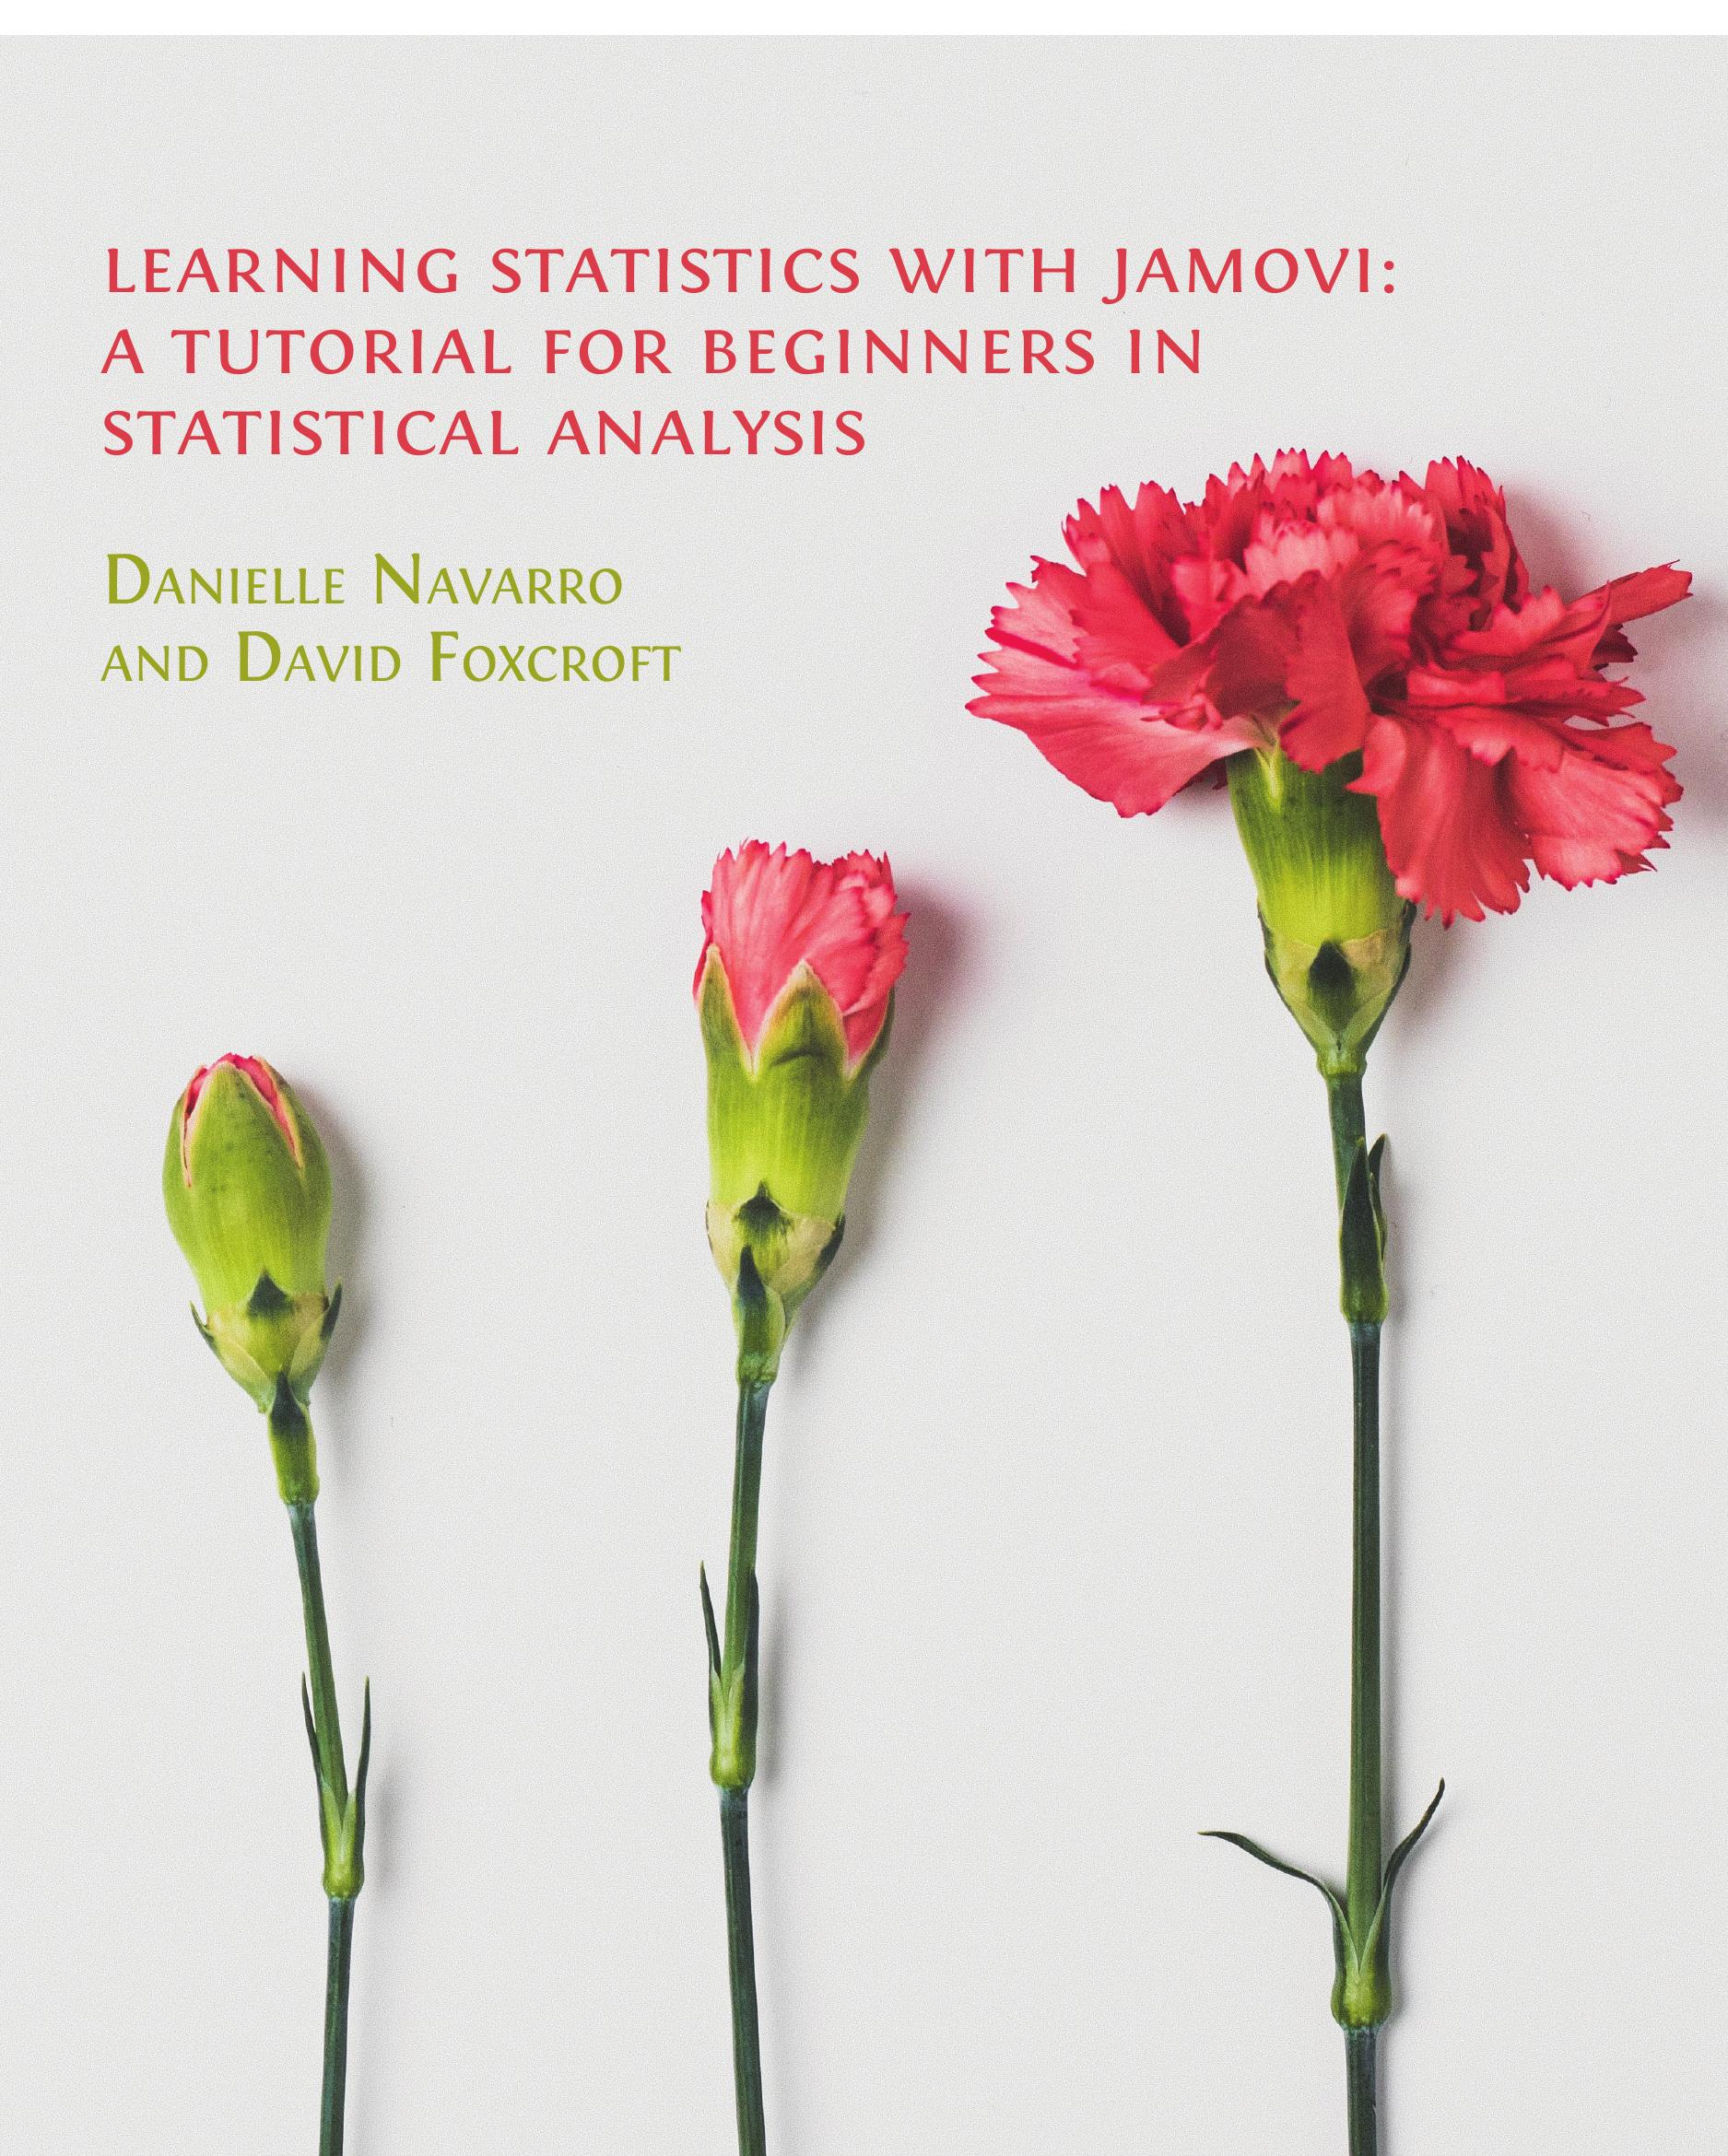
\includepdf[fitpaper=true,pages=-]{images/obp.0333}
\end{center}
\pagestyle{empty}
\let\maketitle\oldmaketitle
\maketitle
\mainmatter
%\pagestyle{plain}
\let\footnote=\endnote

\pagenumbering{roman}
\hspace{0pt}
\vfill
\begin{center}

\Huge{Learning Statistics with jamovi}

\Large{A Tutorial for Beginners in Statistical Analysis}\\*[20pt]

\normalsize{Danielle Navarro and David Foxcroft}

\vfill
\end{center}
\hspace{0pt}
\pagebreak

\hspace{0pt}
\vfill

\copyright 2025 David Foxcroft and Danielle Navarro

This work is licensed under an Attribution-ShareAlike 4.0 International (CC BY-SA 4.0).

This license allows you to copy and redistribute, transform, and build upon the material for any purpose, even commercially. providing attribution is made to the authors (but not in any way that suggests that they endorse you or your use of the work). Attribution should include the following information:

Danielle Navarro and David Foxcroft, \textit{Learning statistics with jamovi: A tutorial for beginners in statistical analysis}. Cambridge, UK: Open Book Publishers, 2025, \url{https://doi.org/10.11647/OBP.0333}

Further details about CC BY-SA licenses are available at \\ \url{https://creativecommons.org/licenses/by-sa/4.0/}

All external links were active at the time of publication unless otherwise stated and have been archived via the Internet Archive Wayback Machine at \\ \url{https://archive.org/web}

Digital material and resources associated with this volume are available at \\ \url{https://doi.org/10.11647/OBP.0333\#resources}

ISBN Paperback: 978-1-80064-937-8

ISBN Hardback: 978-1-80064-938-5

ISBN Digital (PDF): 978-1-80064-939-2

DOI: 10.11647/OBP.0333


\vfill
\hspace{0pt}
\pagebreak

\hspace{0pt}
\vfill

This textbook covers the contents of an introductory statistics class, as typically taught to undergraduate psychology, health or social science students. The book covers how to get started in jamovi as well as giving an introduction to data manipulation. From a statistical perspective, the book discusses descriptive statistics and graphing first, followed by chapters on probability theory, sampling and estimation, and null hypothesis testing. After introducing the theory, the book covers the analysis of contingency tables, correlation, \textit{t}-tests, regression, ANOVA and factor analysis. Bayesian statistics are touched on at the end of the book.

Data sets used in the book are freely available for use in jamovi. All the data files you need can be accessed within jamovi via an add-on module in the jamovi library. Or you can download the files from \url{https://www.learnstatswithjamovi.com}.


Citation: Danielle Navarro and David Foxcroft, \textit{Learning statistics with jamovi: A tutorial for beginners in statistical analysis}. Cambridge, UK: Open Book Publishers, 2025, \url{https://doi.org/10.11647/OBP.0333}

\vfill
\hspace{0pt}

\ifdefined\Shaded\renewenvironment{Shaded}{\begin{tcolorbox}[boxrule=0pt, frame hidden, breakable, sharp corners, interior hidden, enhanced, borderline west={3pt}{0pt}{shadecolor}]}{\end{tcolorbox}}\fi

\renewcommand*\contentsname{Table of contents}
{
\hypersetup{linkcolor=}
\setcounter{tocdepth}{2}
\tableofcontents
}
\mainmatter
\bookmarksetup{startatroot}

\hypertarget{preface-to-version-1.00}{%
\chapter*{Preface to Version 1.00}\label{preface-to-version-1.00}}
\addcontentsline{toc}{chapter}{Preface to Version 1.00}

\markboth{Preface to Version 1.00}{Preface to Version 1.00}

This book is an adaptation of DJ Navarro (2018). Learning statistics
with R: A tutorial for psychology students and other beginners. (Version
0.6). \url{https://learningstatisticswithr.com/}.

The jamovi version of this book was first released in 2018, as version
0.65. Versions 0.70 and 0.75 were released in subsequent years with
corrections and additions. In that time, many people have contacted us
asking for a hard copy version of the book. To achieve this, and to
preserve the open source attributes of the book and materials, we have
worked with
\href{https://www.openbookpublishers.com/books/10.11647/obp.0333}{Open
Book Publishers} in Cambridge, UK, to release this updated version. Open
Book Publishers are the leading independent open access publisher of
academic research in the Humanities and Social Sciences in the UK. They
are award-winning, not-for-profit, run by scholars, and committed to
making high-quality research freely available to readers around the
world.

\emph{David Foxcroft\\
January 1st, 2025}

\bookmarksetup{startatroot}

\hypertarget{sec-Correlation-and-linear-regression}{%
\chapter{Correlation and linear
regression}\label{sec-Correlation-and-linear-regression}}

The goal in this chapter is to introduce \textbf{correlation} and
\textbf{linear regression}. These are the standard tools that
statisticians rely on when analysing the relationship between continuous
predictors and continuous outcomes.

\hypertarget{correlations}{%
\section{Correlations}\label{correlations}}

In this section we'll talk about how to describe the relationships
between variables in the data. To do that, we want to talk mostly about
the \textbf{correlation} between variables. But first, we need some data
(Table~\ref{tbl-tab12-1}).

\hypertarget{the-data}{%
\subsection{The data}\label{the-data}}

\hypertarget{tbl-tab12-1}{}
 
  \providecommand{\huxb}[2]{\arrayrulecolor[RGB]{#1}\global\arrayrulewidth=#2pt}
  \providecommand{\huxvb}[2]{\color[RGB]{#1}\vrule width #2pt}
  \providecommand{\huxtpad}[1]{\rule{0pt}{#1}}
  \providecommand{\huxbpad}[1]{\rule[-#1]{0pt}{#1}}

\begin{table}[ht]
\caption{\label{tbl-tab12-1}Data for correlation analysis - descriptive statistics for the
\emph{parenthood} data }\tabularnewline

\begin{centerbox}
\begin{threeparttable}
\setlength{\tabcolsep}{0pt}
\begin{tabularx}{0.9\textwidth}{p{0.128571428571429\textwidth} p{0.128571428571429\textwidth} p{0.128571428571429\textwidth} p{0.128571428571429\textwidth} p{0.128571428571429\textwidth} p{0.128571428571429\textwidth} p{0.128571428571429\textwidth}}


\hhline{>{\huxb{0, 0, 0}{0.4}}->{\huxb{0, 0, 0}{0.4}}->{\huxb{0, 0, 0}{0.4}}->{\huxb{0, 0, 0}{0.4}}->{\huxb{0, 0, 0}{0.4}}->{\huxb{0, 0, 0}{0.4}}->{\huxb{0, 0, 0}{0.4}}-}
\arrayrulecolor{black}

\multicolumn{1}{!{\huxvb{0, 0, 0}{0}}p{0.128571428571429\textwidth}!{\huxvb{0, 0, 0}{0}}}{\hspace{0pt}\parbox[b]{0.128571428571429\textwidth-0pt-12pt}{\huxtpad{2pt + 1em}\centering \textbf{variable}\huxbpad{2pt}}} &
\multicolumn{1}{p{0.128571428571429\textwidth}!{\huxvb{0, 0, 0}{0}}}{\hspace{12pt}\parbox[b]{0.128571428571429\textwidth-12pt-12pt}{\huxtpad{2pt + 1em}\centering \textbf{min}\huxbpad{2pt}}} &
\multicolumn{1}{p{0.128571428571429\textwidth}!{\huxvb{0, 0, 0}{0}}}{\hspace{12pt}\parbox[b]{0.128571428571429\textwidth-12pt-12pt}{\huxtpad{2pt + 1em}\centering \textbf{max}\huxbpad{2pt}}} &
\multicolumn{1}{p{0.128571428571429\textwidth}!{\huxvb{0, 0, 0}{0}}}{\hspace{12pt}\parbox[b]{0.128571428571429\textwidth-12pt-12pt}{\huxtpad{2pt + 1em}\centering \textbf{mean}\huxbpad{2pt}}} &
\multicolumn{1}{p{0.128571428571429\textwidth}!{\huxvb{0, 0, 0}{0}}}{\hspace{12pt}\parbox[b]{0.128571428571429\textwidth-12pt-12pt}{\huxtpad{2pt + 1em}\centering \textbf{median}\huxbpad{2pt}}} &
\multicolumn{1}{p{0.128571428571429\textwidth}!{\huxvb{0, 0, 0}{0}}}{\hspace{12pt}\parbox[b]{0.128571428571429\textwidth-12pt-12pt}{\huxtpad{2pt + 1em}\centering \textbf{std. dev}\huxbpad{2pt}}} &
\multicolumn{1}{p{0.128571428571429\textwidth}!{\huxvb{0, 0, 0}{0}}}{\hspace{12pt}\parbox[b]{0.128571428571429\textwidth-12pt-0pt}{\huxtpad{2pt + 1em}\centering \textbf{IQR}\huxbpad{2pt}}} \tabularnewline[-0.5pt]


\hhline{>{\huxb{0, 0, 0}{0.4}}->{\huxb{0, 0, 0}{0.4}}->{\huxb{0, 0, 0}{0.4}}->{\huxb{0, 0, 0}{0.4}}->{\huxb{0, 0, 0}{0.4}}->{\huxb{0, 0, 0}{0.4}}->{\huxb{0, 0, 0}{0.4}}-}
\arrayrulecolor{black}

\multicolumn{1}{!{\huxvb{0, 0, 0}{0}}p{0.128571428571429\textwidth}!{\huxvb{0, 0, 0}{0}}}{\hspace{0pt}\parbox[b]{0.128571428571429\textwidth-0pt-12pt}{\huxtpad{2pt + 1em}\centering Dani's grumpiness\huxbpad{2pt}}} &
\multicolumn{1}{p{0.128571428571429\textwidth}!{\huxvb{0, 0, 0}{0}}}{\hspace{12pt}\parbox[b]{0.128571428571429\textwidth-12pt-12pt}{\huxtpad{2pt + 1em}\centering 41\huxbpad{2pt}}} &
\multicolumn{1}{p{0.128571428571429\textwidth}!{\huxvb{0, 0, 0}{0}}}{\hspace{12pt}\parbox[b]{0.128571428571429\textwidth-12pt-12pt}{\huxtpad{2pt + 1em}\centering 91\huxbpad{2pt}}} &
\multicolumn{1}{p{0.128571428571429\textwidth}!{\huxvb{0, 0, 0}{0}}}{\hspace{12pt}\parbox[b]{0.128571428571429\textwidth-12pt-12pt}{\huxtpad{2pt + 1em}\centering 63.71\huxbpad{2pt}}} &
\multicolumn{1}{p{0.128571428571429\textwidth}!{\huxvb{0, 0, 0}{0}}}{\hspace{12pt}\parbox[b]{0.128571428571429\textwidth-12pt-12pt}{\huxtpad{2pt + 1em}\centering 62\huxbpad{2pt}}} &
\multicolumn{1}{p{0.128571428571429\textwidth}!{\huxvb{0, 0, 0}{0}}}{\hspace{12pt}\parbox[b]{0.128571428571429\textwidth-12pt-12pt}{\huxtpad{2pt + 1em}\centering 10.05\huxbpad{2pt}}} &
\multicolumn{1}{p{0.128571428571429\textwidth}!{\huxvb{0, 0, 0}{0}}}{\hspace{12pt}\parbox[b]{0.128571428571429\textwidth-12pt-0pt}{\huxtpad{2pt + 1em}\centering 14\huxbpad{2pt}}} \tabularnewline[-0.5pt]


\hhline{}
\arrayrulecolor{black}

\multicolumn{1}{!{\huxvb{0, 0, 0}{0}}p{0.128571428571429\textwidth}!{\huxvb{0, 0, 0}{0}}}{\hspace{0pt}\parbox[b]{0.128571428571429\textwidth-0pt-12pt}{\huxtpad{2pt + 1em}\centering Dani's hours slept\huxbpad{2pt}}} &
\multicolumn{1}{p{0.128571428571429\textwidth}!{\huxvb{0, 0, 0}{0}}}{\hspace{12pt}\parbox[b]{0.128571428571429\textwidth-12pt-12pt}{\huxtpad{2pt + 1em}\centering 4.84\huxbpad{2pt}}} &
\multicolumn{1}{p{0.128571428571429\textwidth}!{\huxvb{0, 0, 0}{0}}}{\hspace{12pt}\parbox[b]{0.128571428571429\textwidth-12pt-12pt}{\huxtpad{2pt + 1em}\centering 9.00\huxbpad{2pt}}} &
\multicolumn{1}{p{0.128571428571429\textwidth}!{\huxvb{0, 0, 0}{0}}}{\hspace{12pt}\parbox[b]{0.128571428571429\textwidth-12pt-12pt}{\huxtpad{2pt + 1em}\centering 6.97\huxbpad{2pt}}} &
\multicolumn{1}{p{0.128571428571429\textwidth}!{\huxvb{0, 0, 0}{0}}}{\hspace{12pt}\parbox[b]{0.128571428571429\textwidth-12pt-12pt}{\huxtpad{2pt + 1em}\centering 7.03\huxbpad{2pt}}} &
\multicolumn{1}{p{0.128571428571429\textwidth}!{\huxvb{0, 0, 0}{0}}}{\hspace{12pt}\parbox[b]{0.128571428571429\textwidth-12pt-12pt}{\huxtpad{2pt + 1em}\centering 1.02\huxbpad{2pt}}} &
\multicolumn{1}{p{0.128571428571429\textwidth}!{\huxvb{0, 0, 0}{0}}}{\hspace{12pt}\parbox[b]{0.128571428571429\textwidth-12pt-0pt}{\huxtpad{2pt + 1em}\centering 1.45\huxbpad{2pt}}} \tabularnewline[-0.5pt]


\hhline{}
\arrayrulecolor{black}

\multicolumn{1}{!{\huxvb{0, 0, 0}{0}}p{0.128571428571429\textwidth}!{\huxvb{0, 0, 0}{0}}}{\hspace{0pt}\parbox[b]{0.128571428571429\textwidth-0pt-12pt}{\huxtpad{2pt + 1em}\centering Dani's son's hours slept\huxbpad{2pt}}} &
\multicolumn{1}{p{0.128571428571429\textwidth}!{\huxvb{0, 0, 0}{0}}}{\hspace{12pt}\parbox[b]{0.128571428571429\textwidth-12pt-12pt}{\huxtpad{2pt + 1em}\centering 3.25\huxbpad{2pt}}} &
\multicolumn{1}{p{0.128571428571429\textwidth}!{\huxvb{0, 0, 0}{0}}}{\hspace{12pt}\parbox[b]{0.128571428571429\textwidth-12pt-12pt}{\huxtpad{2pt + 1em}\centering 12.07\huxbpad{2pt}}} &
\multicolumn{1}{p{0.128571428571429\textwidth}!{\huxvb{0, 0, 0}{0}}}{\hspace{12pt}\parbox[b]{0.128571428571429\textwidth-12pt-12pt}{\huxtpad{2pt + 1em}\centering 8.05\huxbpad{2pt}}} &
\multicolumn{1}{p{0.128571428571429\textwidth}!{\huxvb{0, 0, 0}{0}}}{\hspace{12pt}\parbox[b]{0.128571428571429\textwidth-12pt-12pt}{\huxtpad{2pt + 1em}\centering 7.95\huxbpad{2pt}}} &
\multicolumn{1}{p{0.128571428571429\textwidth}!{\huxvb{0, 0, 0}{0}}}{\hspace{12pt}\parbox[b]{0.128571428571429\textwidth-12pt-12pt}{\huxtpad{2pt + 1em}\centering 2.07\huxbpad{2pt}}} &
\multicolumn{1}{p{0.128571428571429\textwidth}!{\huxvb{0, 0, 0}{0}}}{\hspace{12pt}\parbox[b]{0.128571428571429\textwidth-12pt-0pt}{\huxtpad{2pt + 1em}\centering 3.21\huxbpad{2pt}}} \tabularnewline[-0.5pt]


\hhline{>{\huxb{0, 0, 0}{0.4}}->{\huxb{0, 0, 0}{0.4}}->{\huxb{0, 0, 0}{0.4}}->{\huxb{0, 0, 0}{0.4}}->{\huxb{0, 0, 0}{0.4}}->{\huxb{0, 0, 0}{0.4}}->{\huxb{0, 0, 0}{0.4}}-}
\arrayrulecolor{black}
\end{tabularx} 

\end{threeparttable}\par\end{centerbox}

\end{table}
 

Let's turn to a topic close to every parent's heart: sleep. The data set
we'll use is fictitious, but based on real events. Suppose I'm curious
to find out how much my infant son's sleeping habits affect my mood.
Let's say that I can rate my grumpiness very precisely, on a scale from
0 (not at all grumpy) to \(100\) (grumpy as a very, very grumpy old man
or woman). And lets also assume that I've been measuring my grumpiness,
my sleeping patterns and my son's sleeping patterns for quite some time
now. Let's say, for \(100\) days. And, being a nerd, I've saved the data
as a file called \emph{parenthood.csv}. If we load the data we can see
that the file contains four variables dani.sleep, baby.sleep, dani.grump
and day. Note that when you first load this data set jamovi may not have
guessed the data type for each variable correctly, in which case you
should fix it: dani.sleep, baby.sleep, dani.grump and day can be
specified as continuous variables, and ID is a nominal(integer)
variable.\footnote{I've noticed that in jamovi you can also specify an
  `ID' variable type, but for our purposes it does not matter how we
  specify the ID variable as we won't be including it in any analyses.}

Next, I'll take a look at some basic descriptive statistics and, to give
a graphical depiction of what each of the three interesting variables
looks like, Figure~\ref{fig-fig12-1} plots histograms. One thing to
note: just because jamovi can calculate dozens of different statistics
doesn't mean you should report all of them. If I were writing this up
for a report, I'd probably pick out those statistics that are of most
interest to me (and to my readership), and then put them into a nice,
simple table like the one in Table 12.1.\footnote{Actually, even that
  table is more than I'd bother with. In practice most people pick one
  measure of central tendency, and one measure of variability only.}
Notice that when I put it into a table, I gave everything ``human
readable'' names. This is always good practice. Notice also that I'm not
getting enough sleep. This isn't good practice, but other parents tell
me that it's pretty standard.

\begin{figure}

\begin{minipage}[b]{0.33\linewidth}

{\centering 

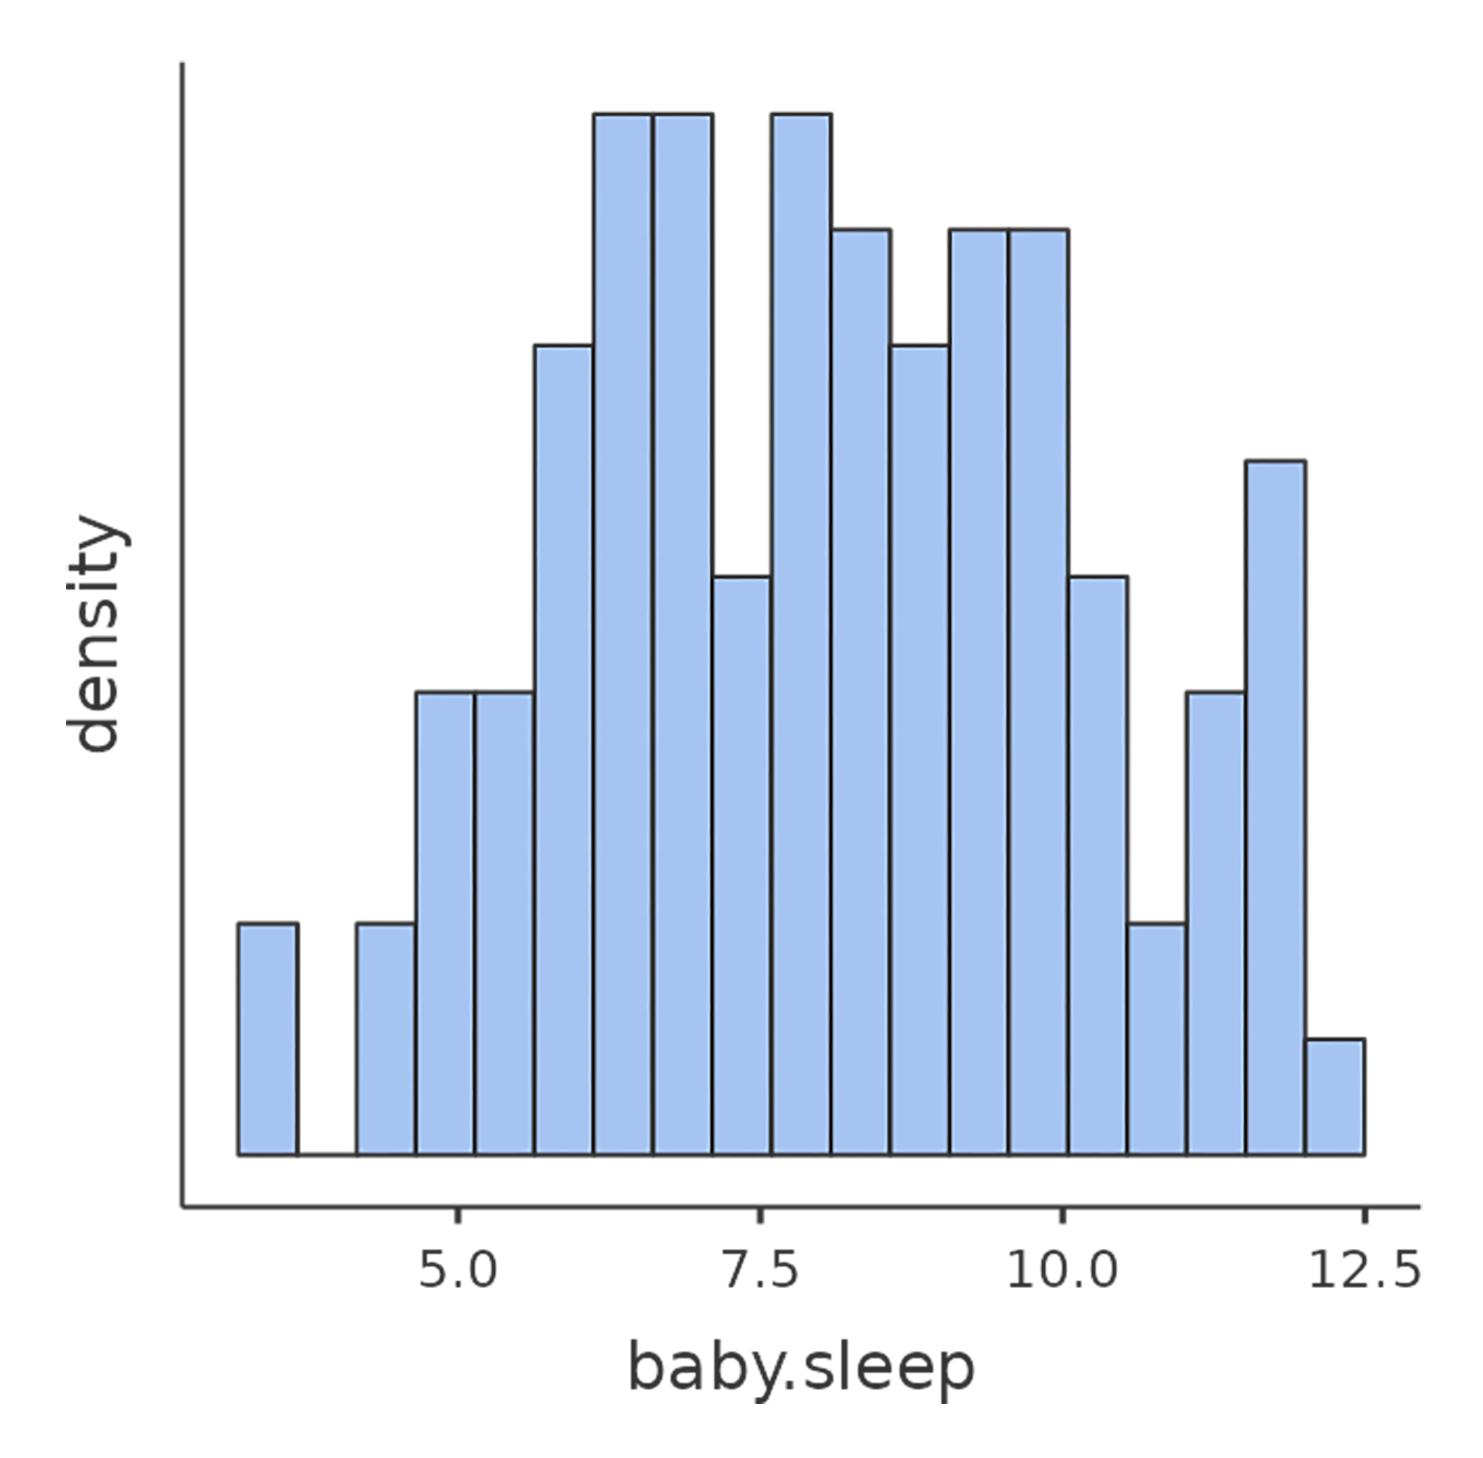
\includegraphics{images/fig12-1a.png}

}

\subcaption{\label{fig-fig12-1a}}
\end{minipage}%
%
\begin{minipage}[b]{0.33\linewidth}

{\centering 

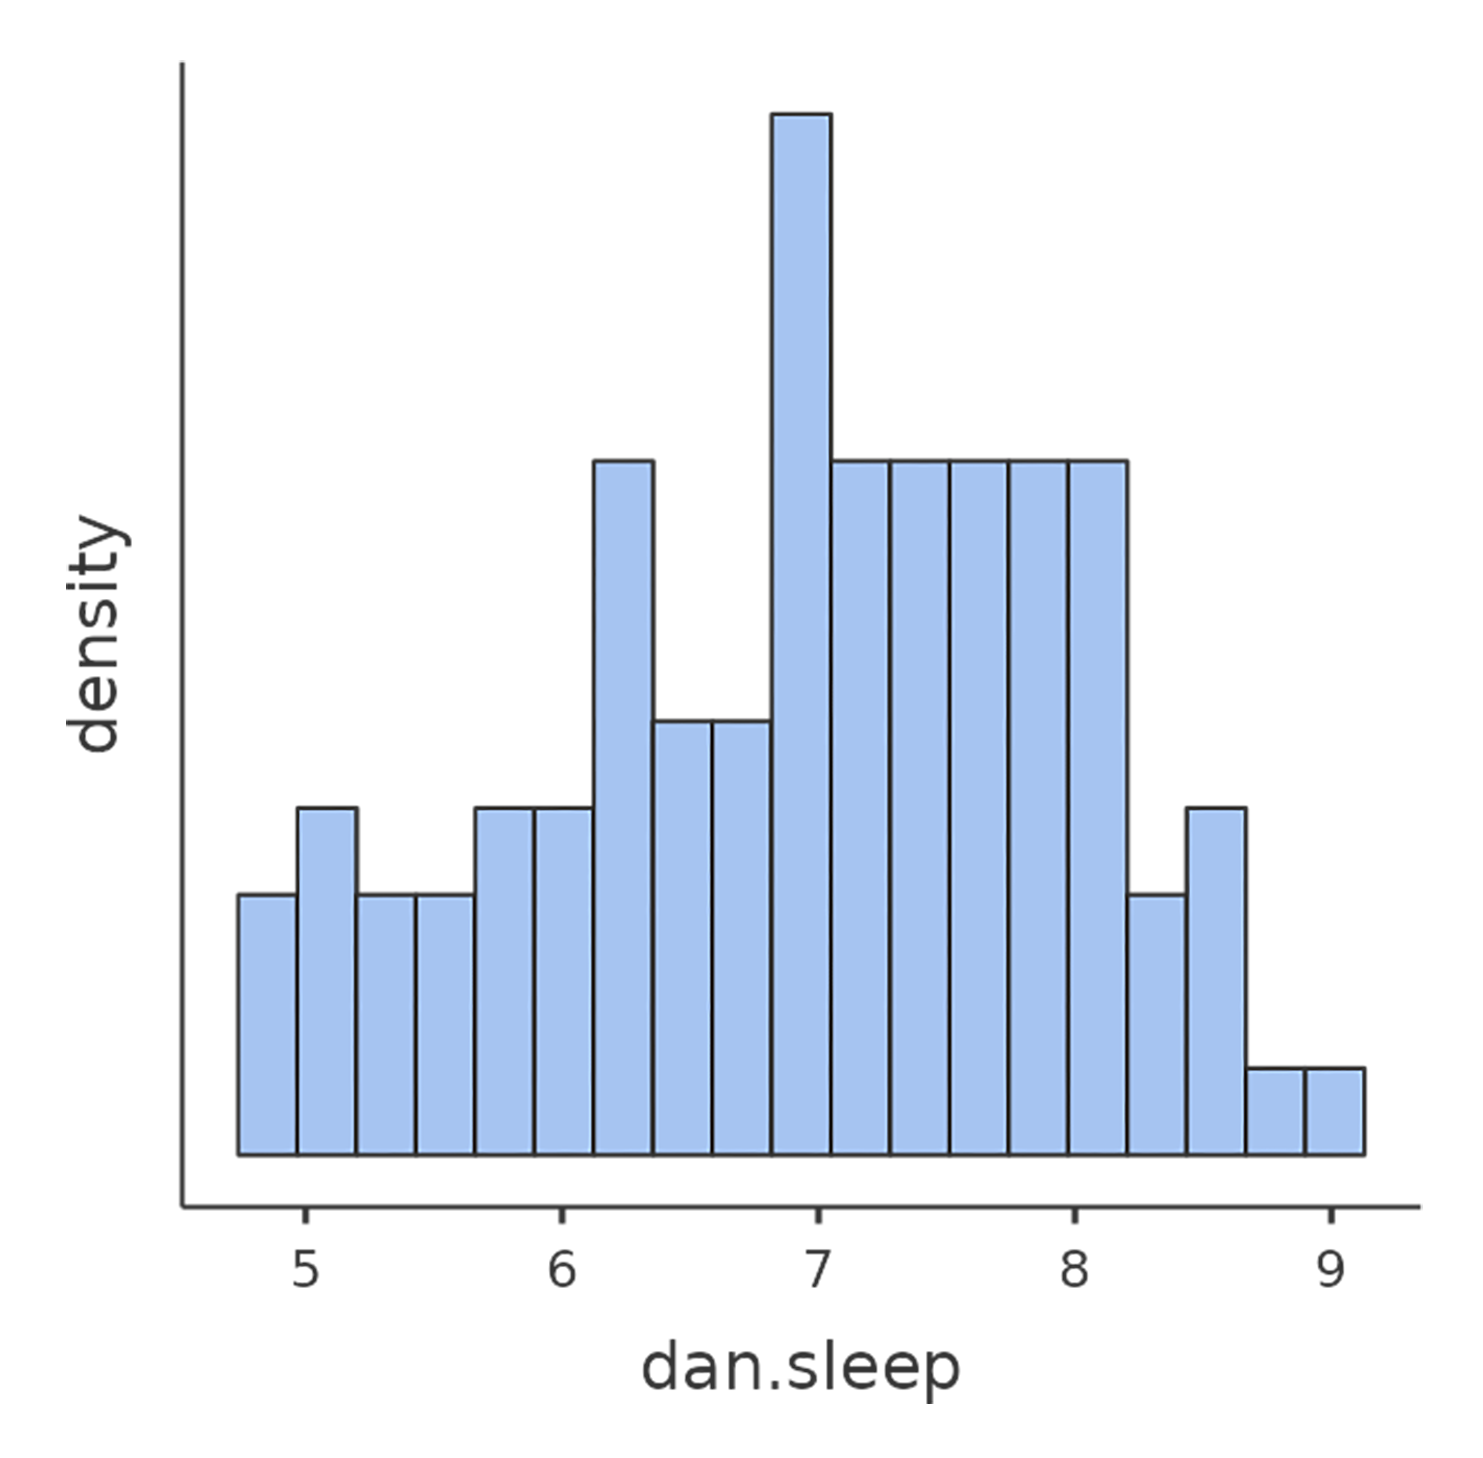
\includegraphics{images/fig12-1b.png}

}

\subcaption{\label{fig-fig12-1b}}
\end{minipage}%
%
\begin{minipage}[b]{0.33\linewidth}

{\centering 

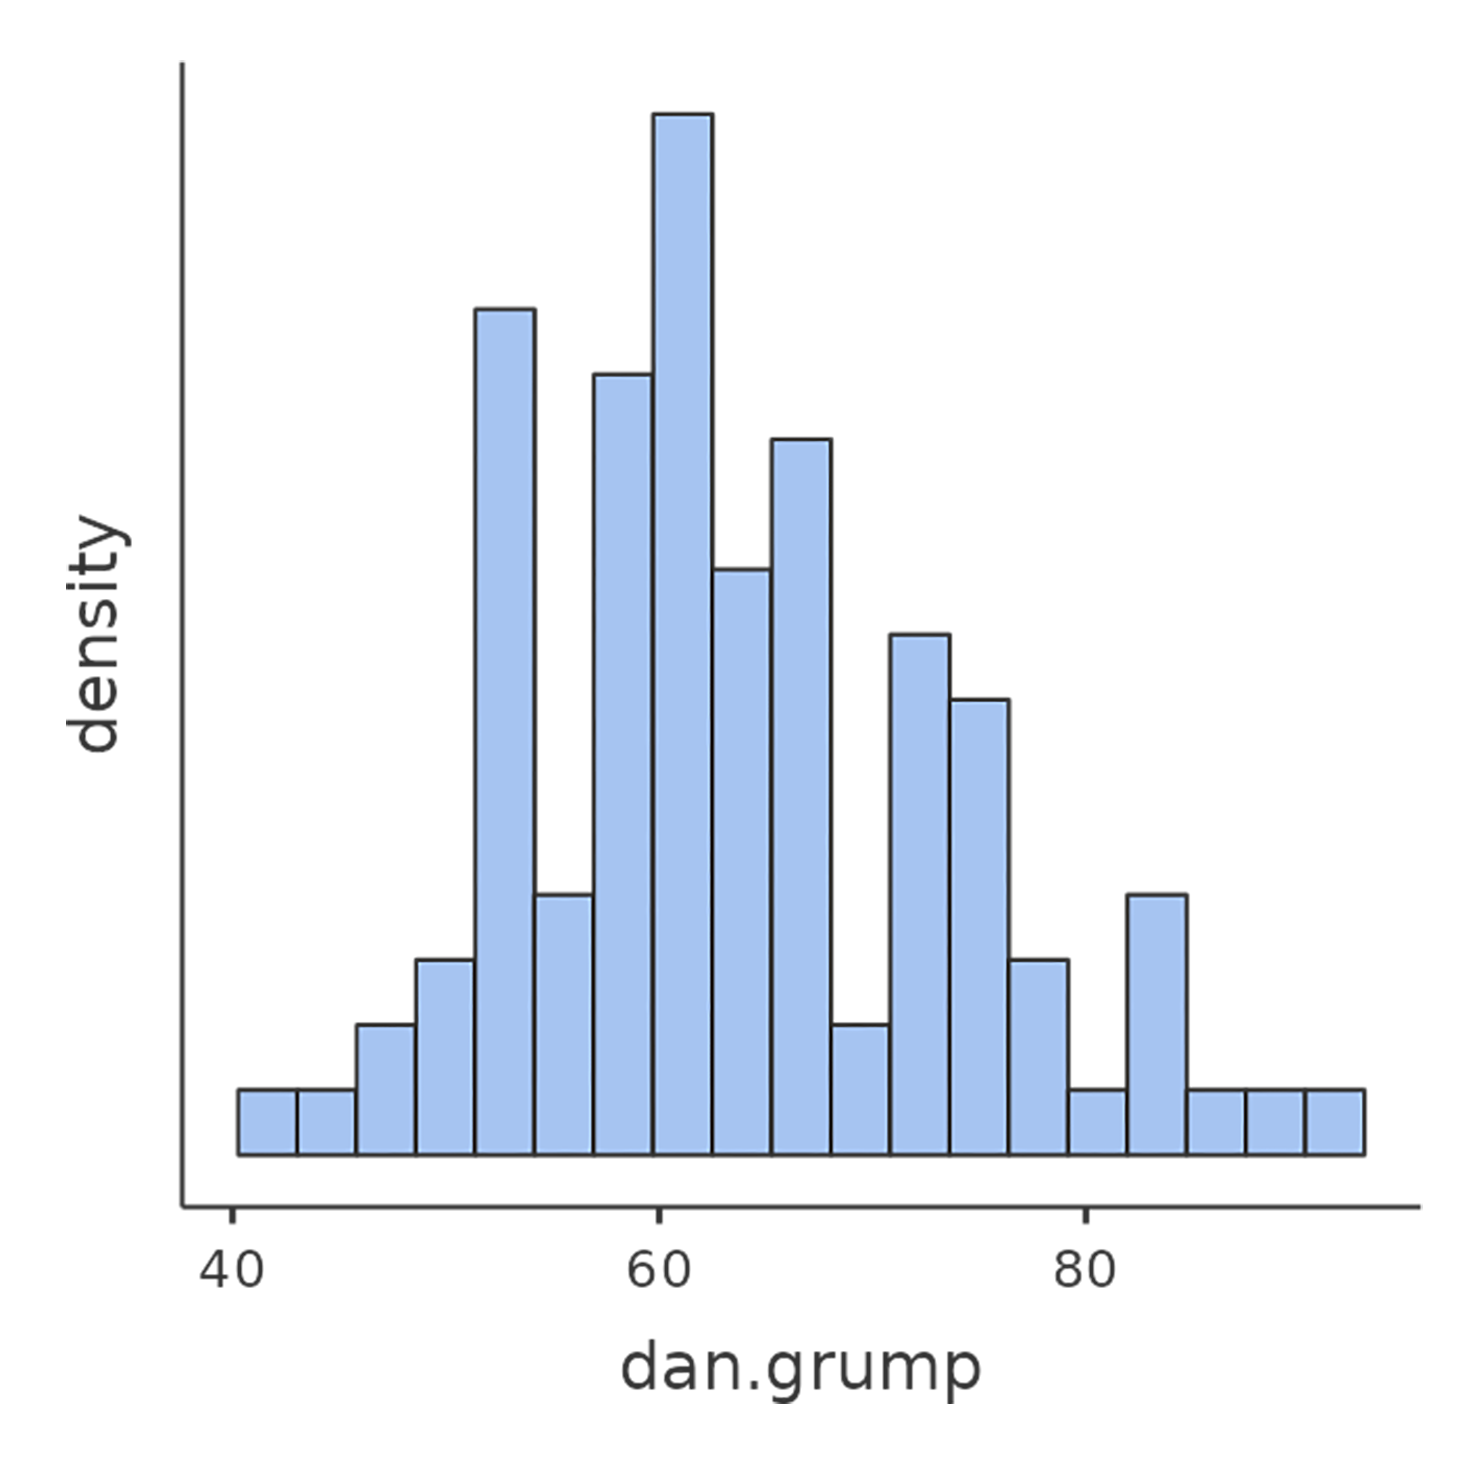
\includegraphics{images/fig12-1c.png}

}

\subcaption{\label{fig-fig12-1c}}
\end{minipage}%

\caption{\label{fig-fig12-1}Histograms from jamovi for the three
interesting variables in the \emph{parenthood}data set}

\end{figure}

\hypertarget{the-strength-and-direction-of-a-relationship}{%
\subsection{The strength and direction of a
relationship}\label{the-strength-and-direction-of-a-relationship}}

We can draw scatterplots to give us a general sense of how closely
related two variables are. Ideally though, we might want to say a bit
more about it than that. For instance, let's compare the relationship
between baby.sleep and dani.grump (Figure~\ref{fig-fig12-1a}), left,
with that between dani.sleep and dani.grump (Figure~\ref{fig-fig12-1b}),
right. When looking at these two plots side by side, it's clear that the
relationship is qualitatively the same in both cases: more sleep equals
less grump! However, it's also pretty obvious that the relationship
between dani.sleep and dani.grump is stronger than the relationship
between baby.sleep and dani.grump. The plot on the right is ``neater''
than the one on the left. What it feels like is that if you want to
predict what my mood is, it'd help you a little bit to know how many
hours my son slept, but it'd be more helpful to know how many hours I
slept.

\begin{figure}

\begin{minipage}[b]{0.50\linewidth}

{\centering 

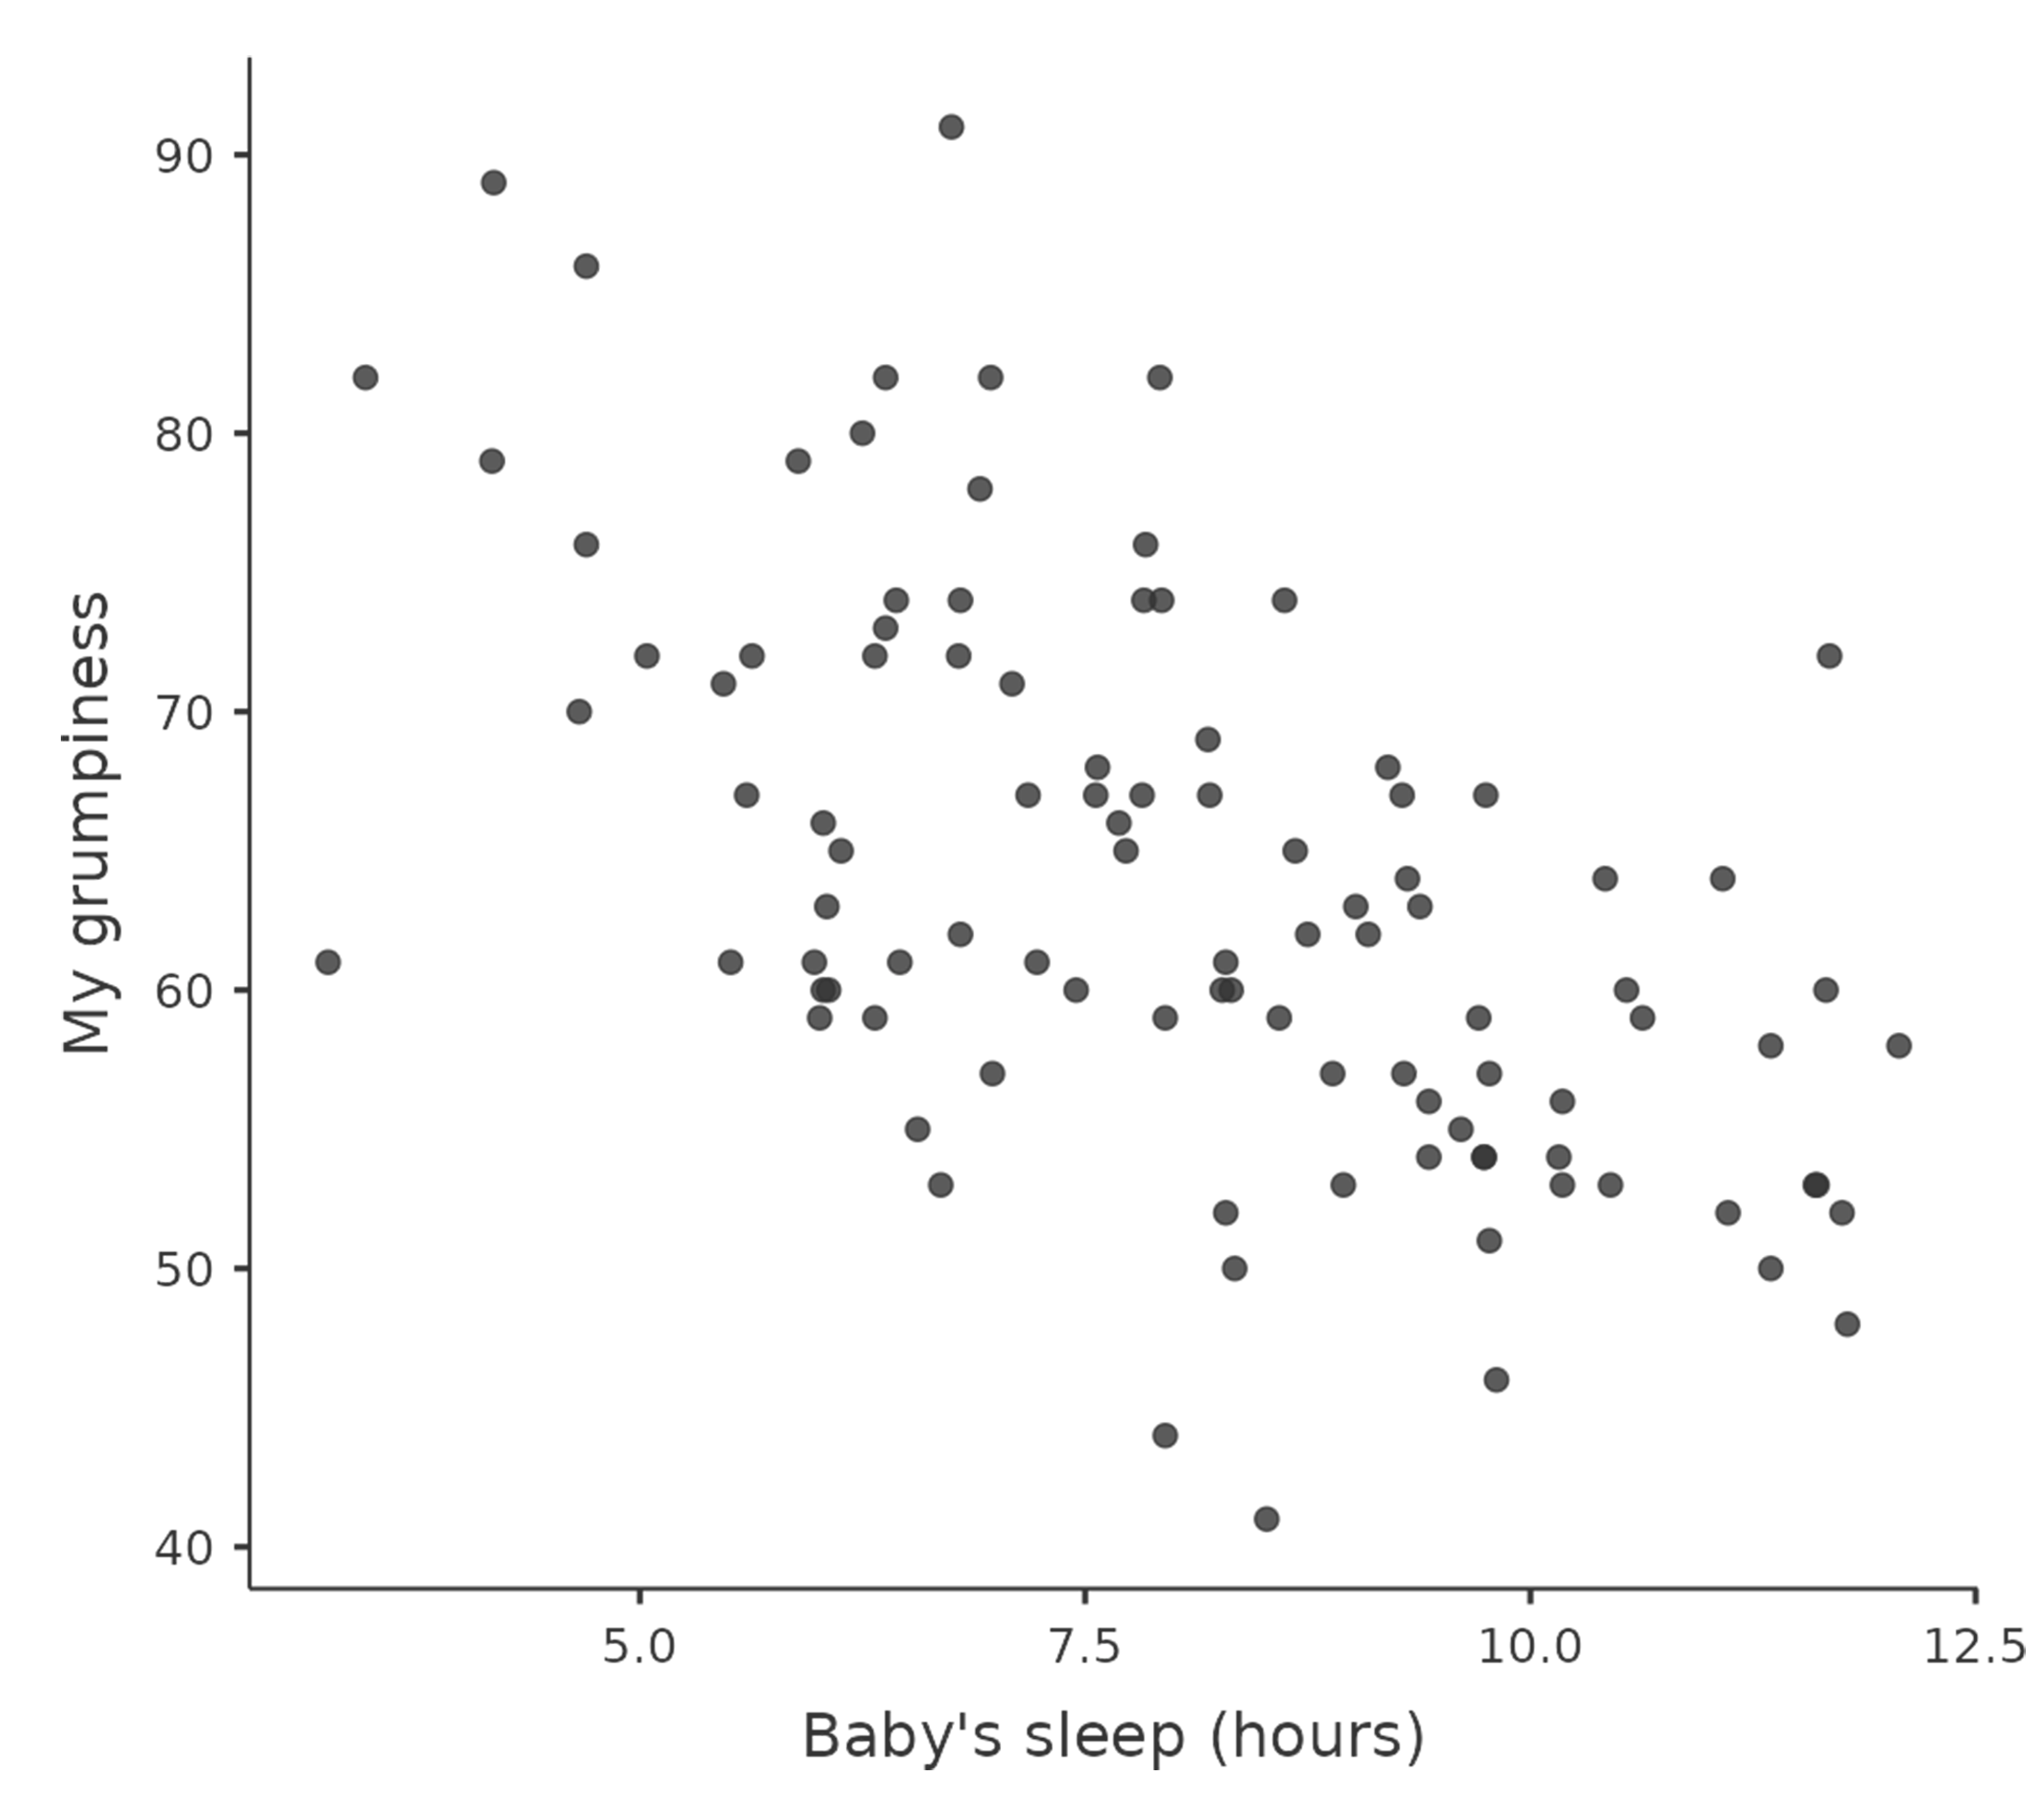
\includegraphics{images/fig12-2a.png}

}

\subcaption{\label{fig-fig12-2a}}
\end{minipage}%
%
\begin{minipage}[b]{0.50\linewidth}

{\centering 

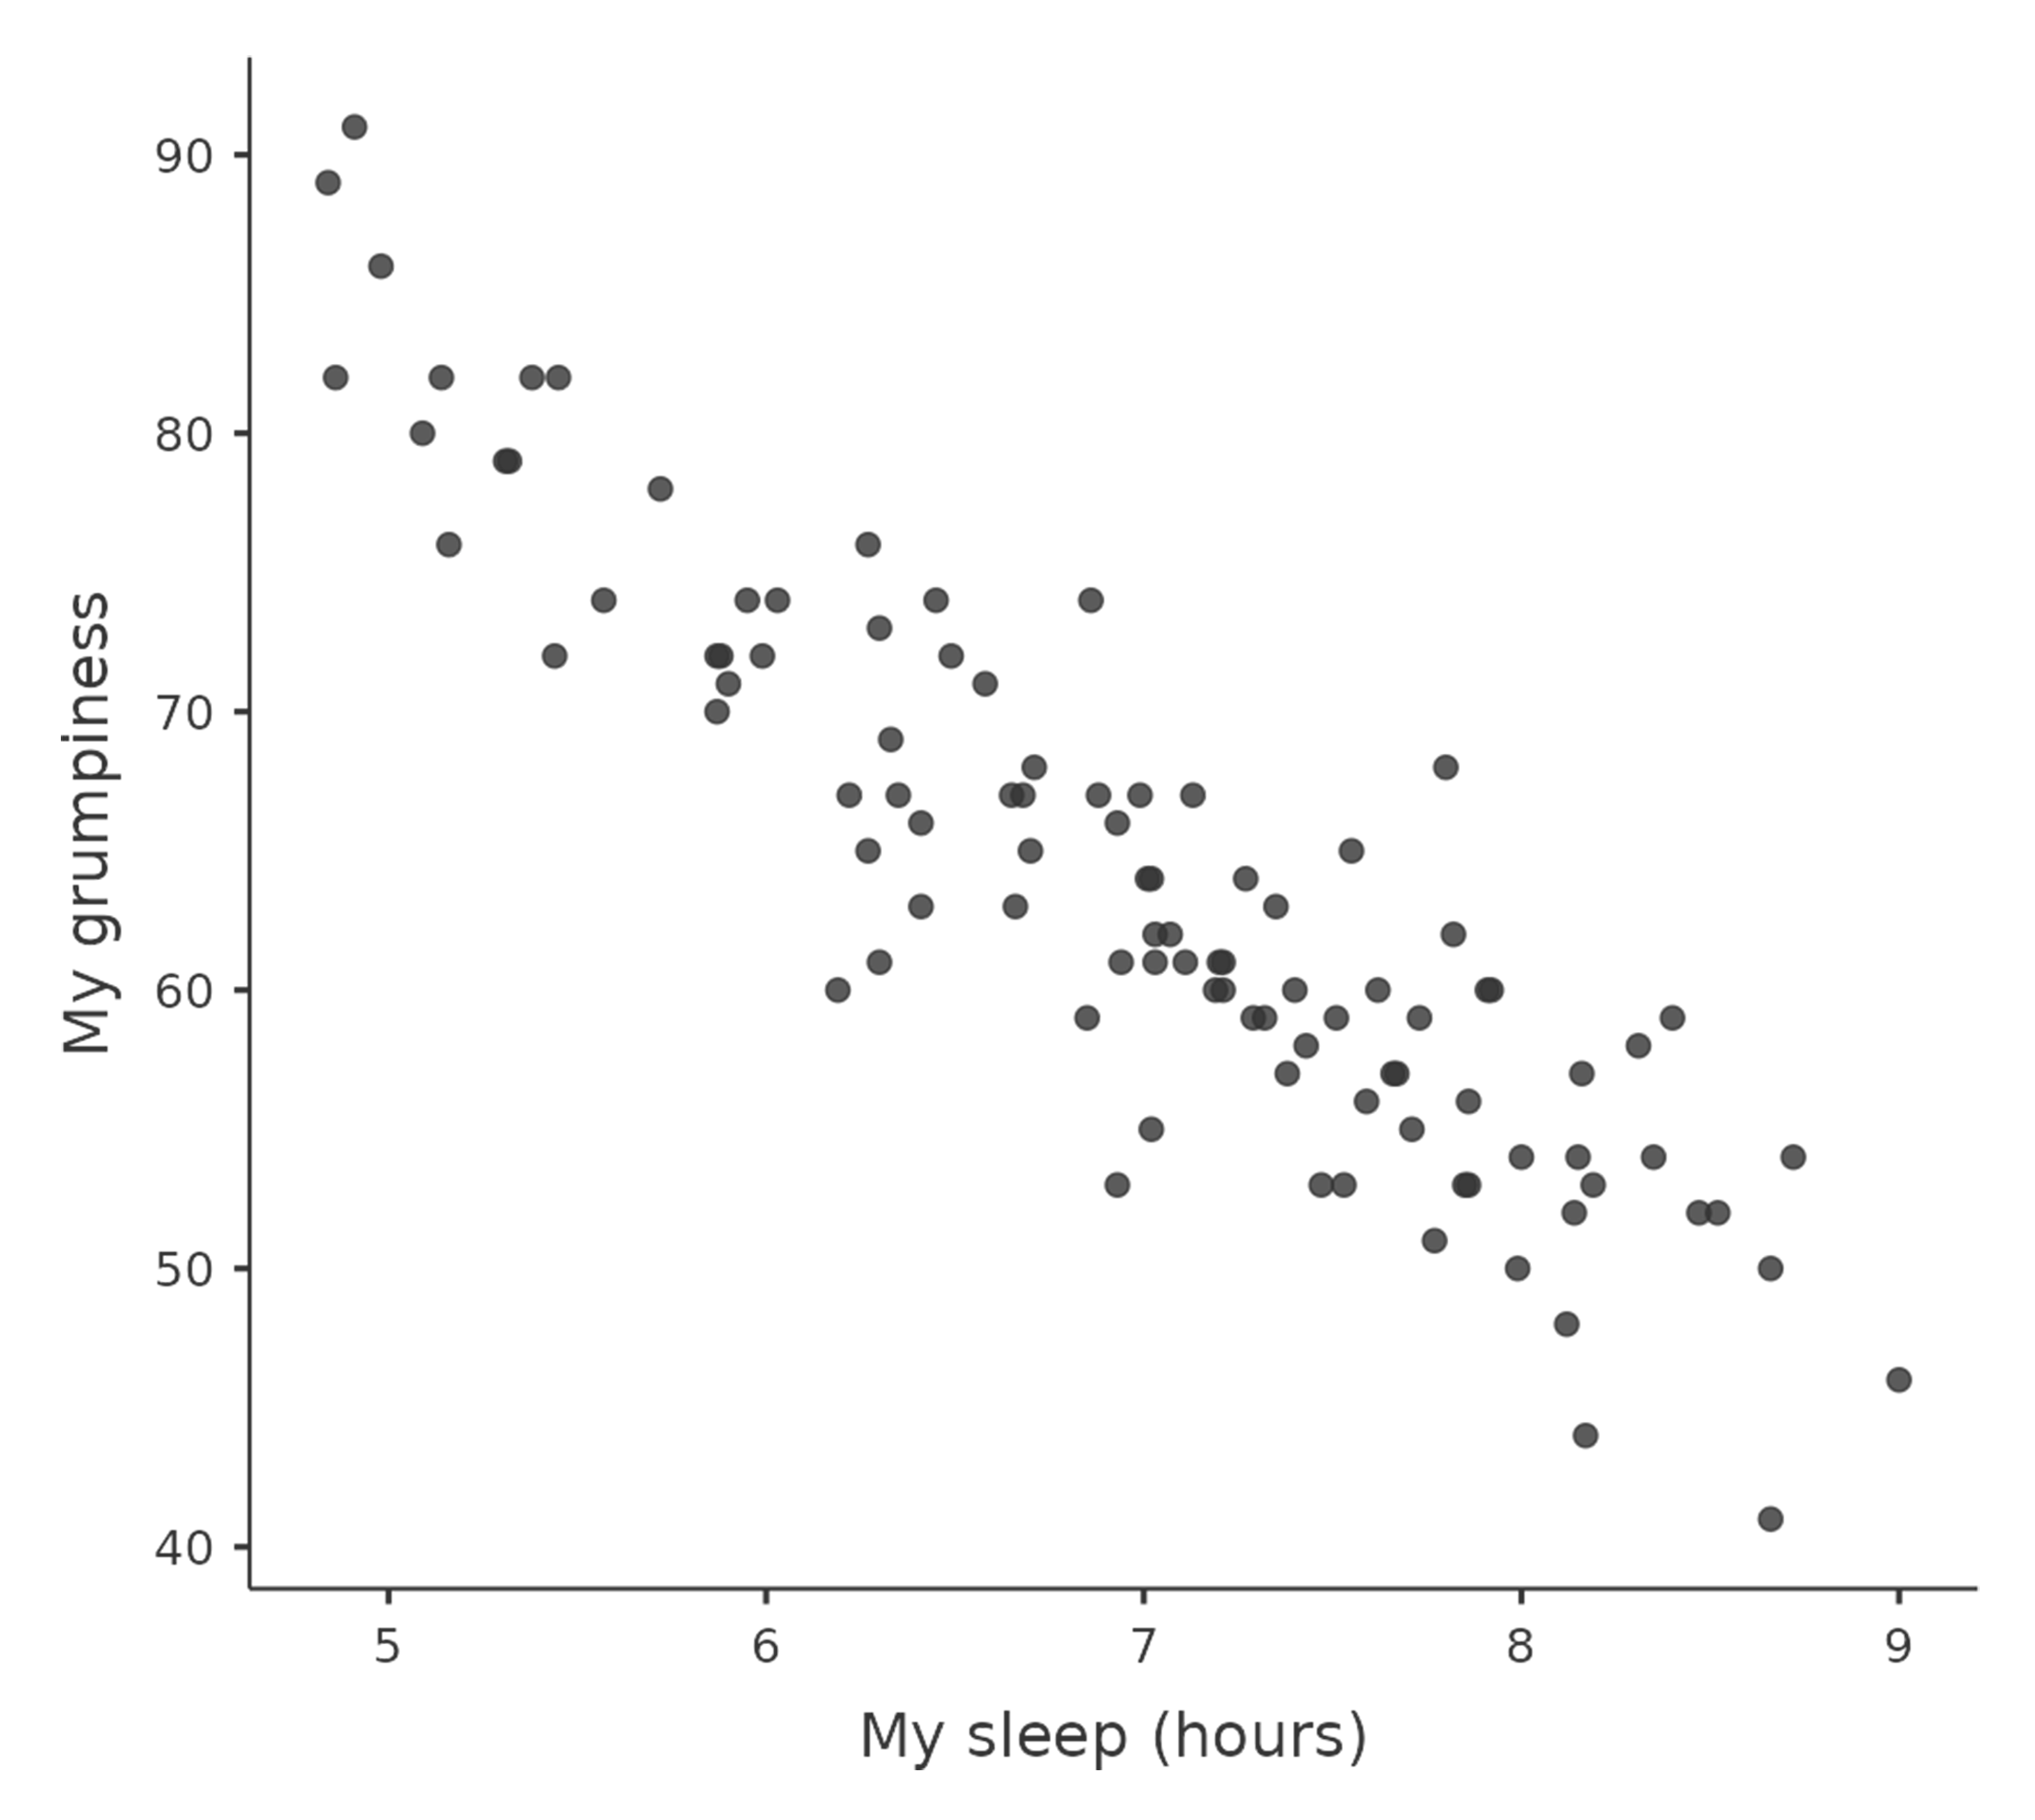
\includegraphics{images/fig12-2b.png}

}

\subcaption{\label{fig-fig12-2b}}
\end{minipage}%

\caption{\label{fig-fig12-2}Scatterplots from jamovi showing the
relationship between baby.sleep and dani.grump (left) and the
relationship between dani.sleep and dani.grump (right)}

\end{figure}

In contrast, let's consider the two scatterplots shown in
Figure~\ref{fig-fig12-3}. If we compare the scatterplot of ``baby.sleep
v dani.grump'' (left) to the scatterplot of ``baby.sleep v dani.sleep''
(right), the overall strength of the relationship is the same, but the
direction is different. That is, if my son sleeps more, I get more sleep
(positive relationship, right-hand side), but if he sleeps more then I
get less grumpy (negative relationship, left-hand side).

\begin{figure}

\begin{minipage}[b]{0.50\linewidth}

{\centering 

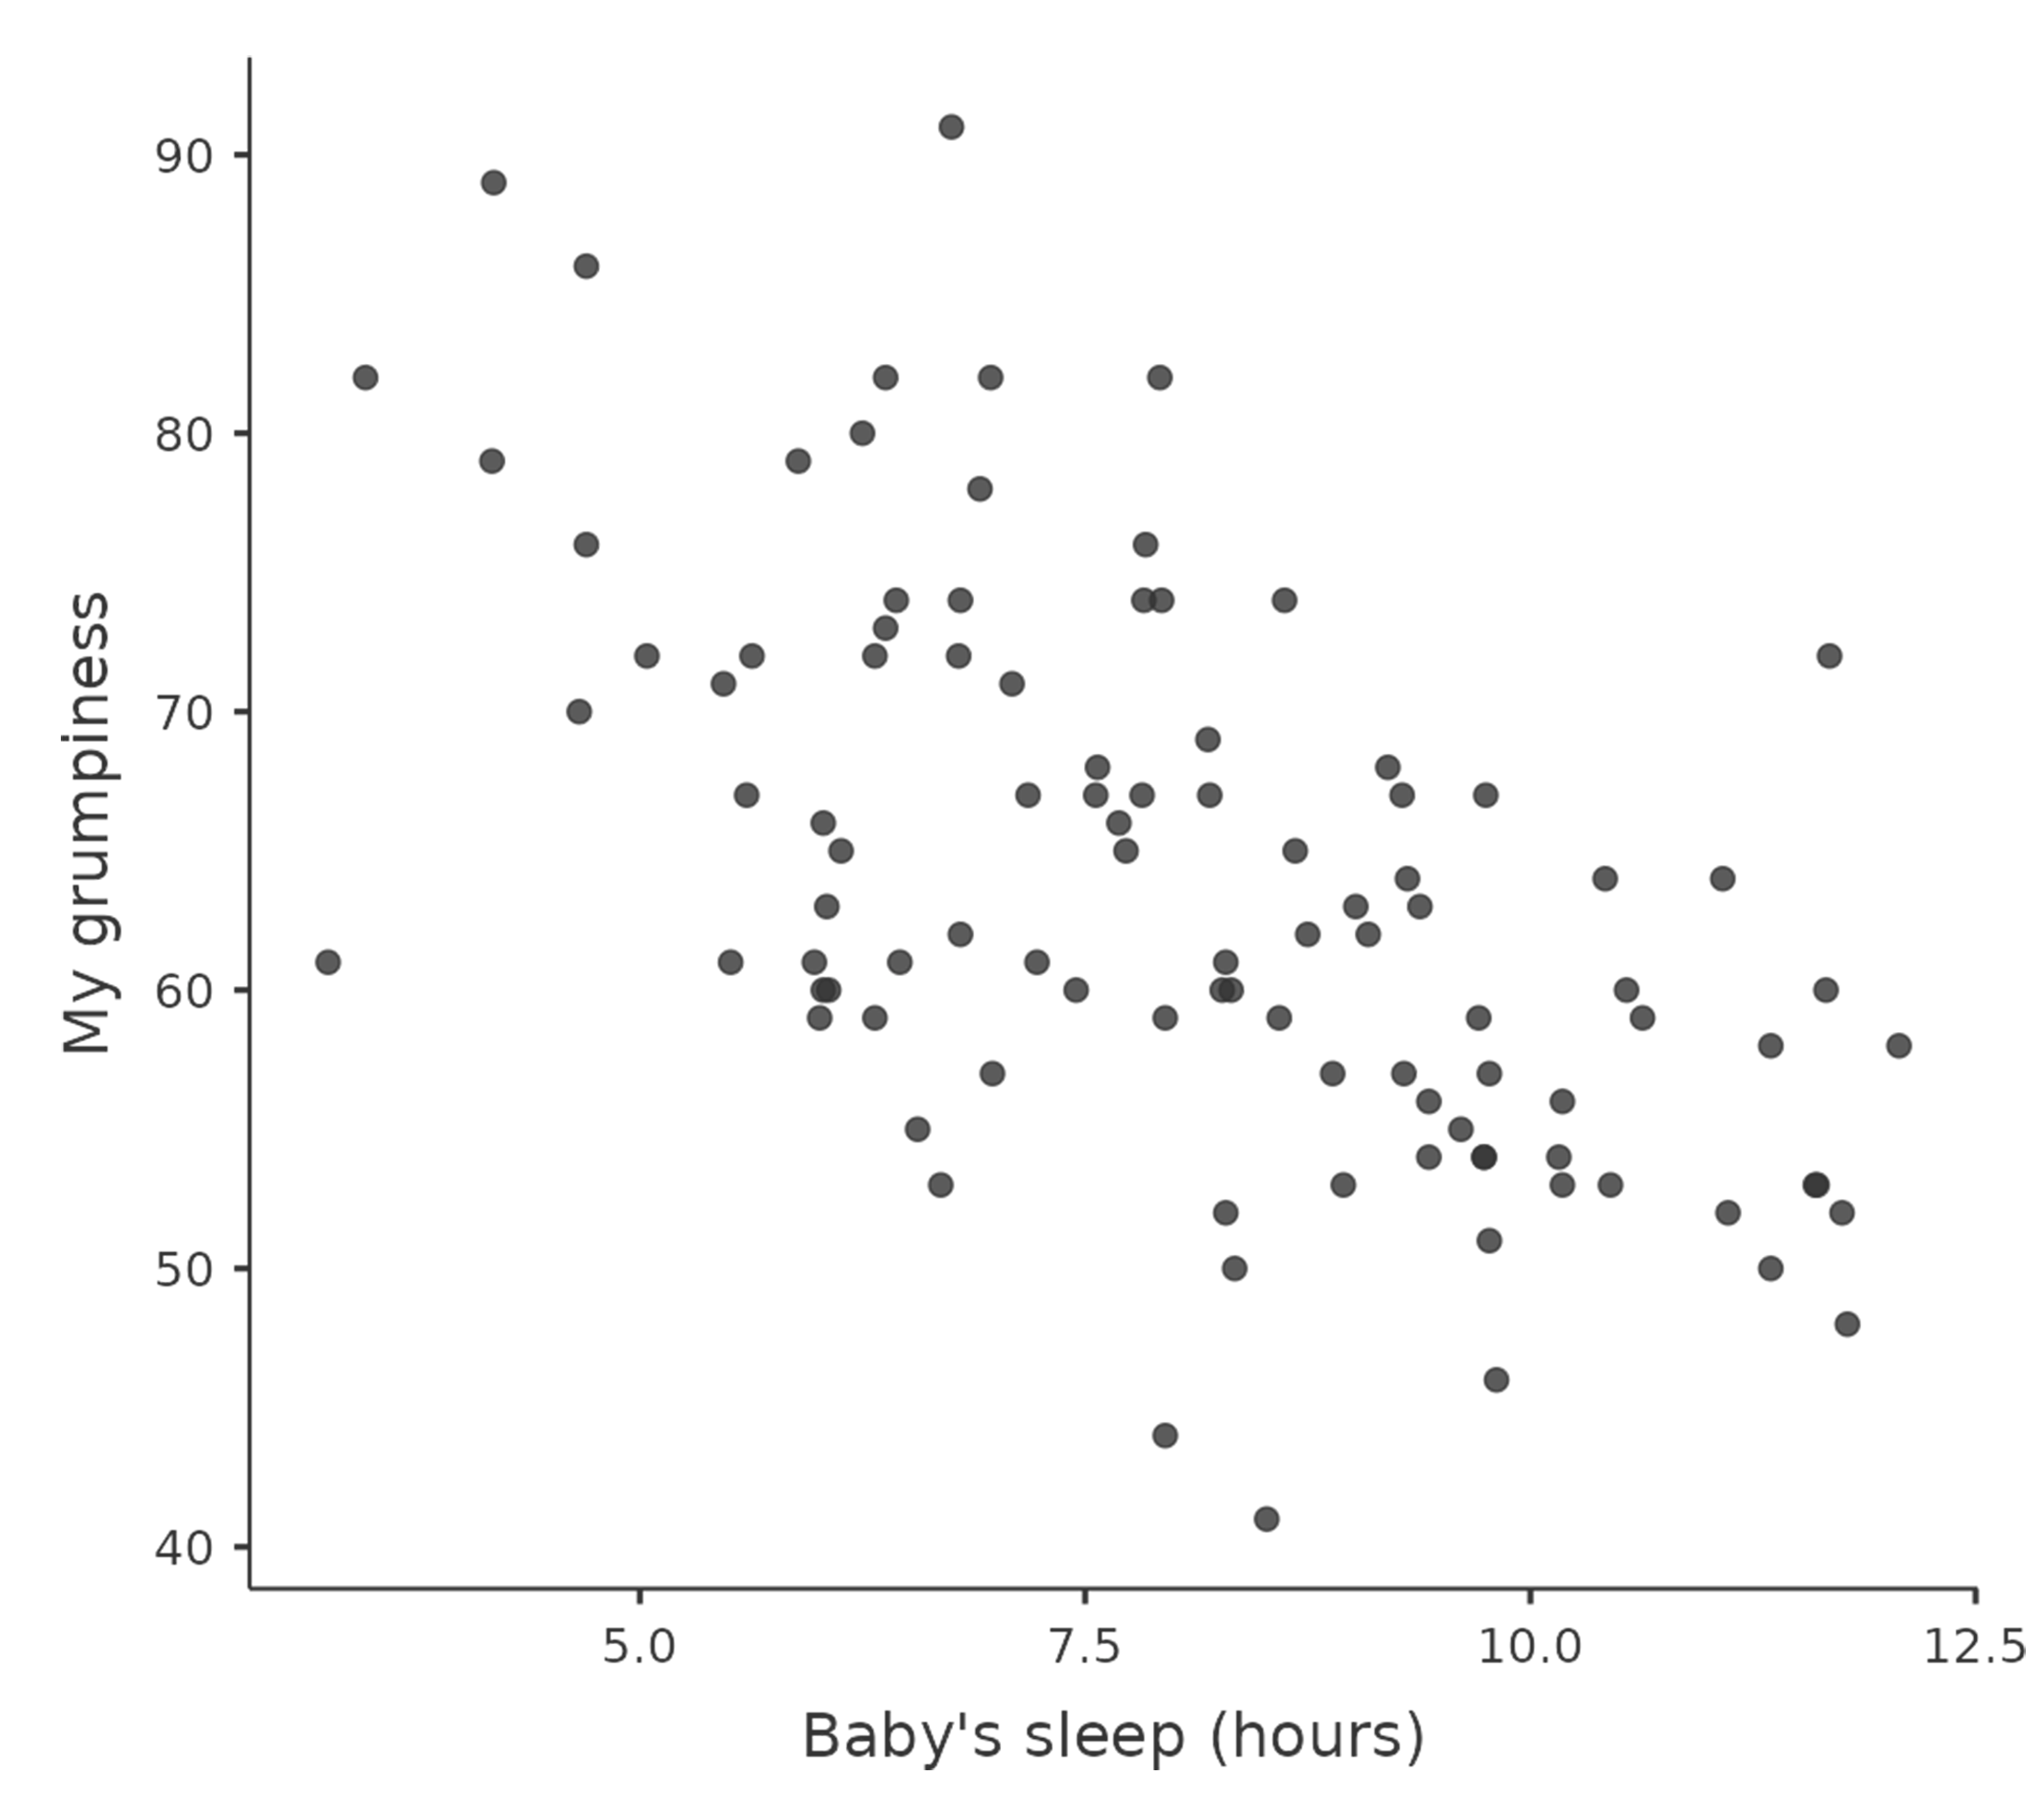
\includegraphics{images/fig12-2a.png}

}

\subcaption{\label{fig-fig12-3a}}
\end{minipage}%
%
\begin{minipage}[b]{0.50\linewidth}

{\centering 

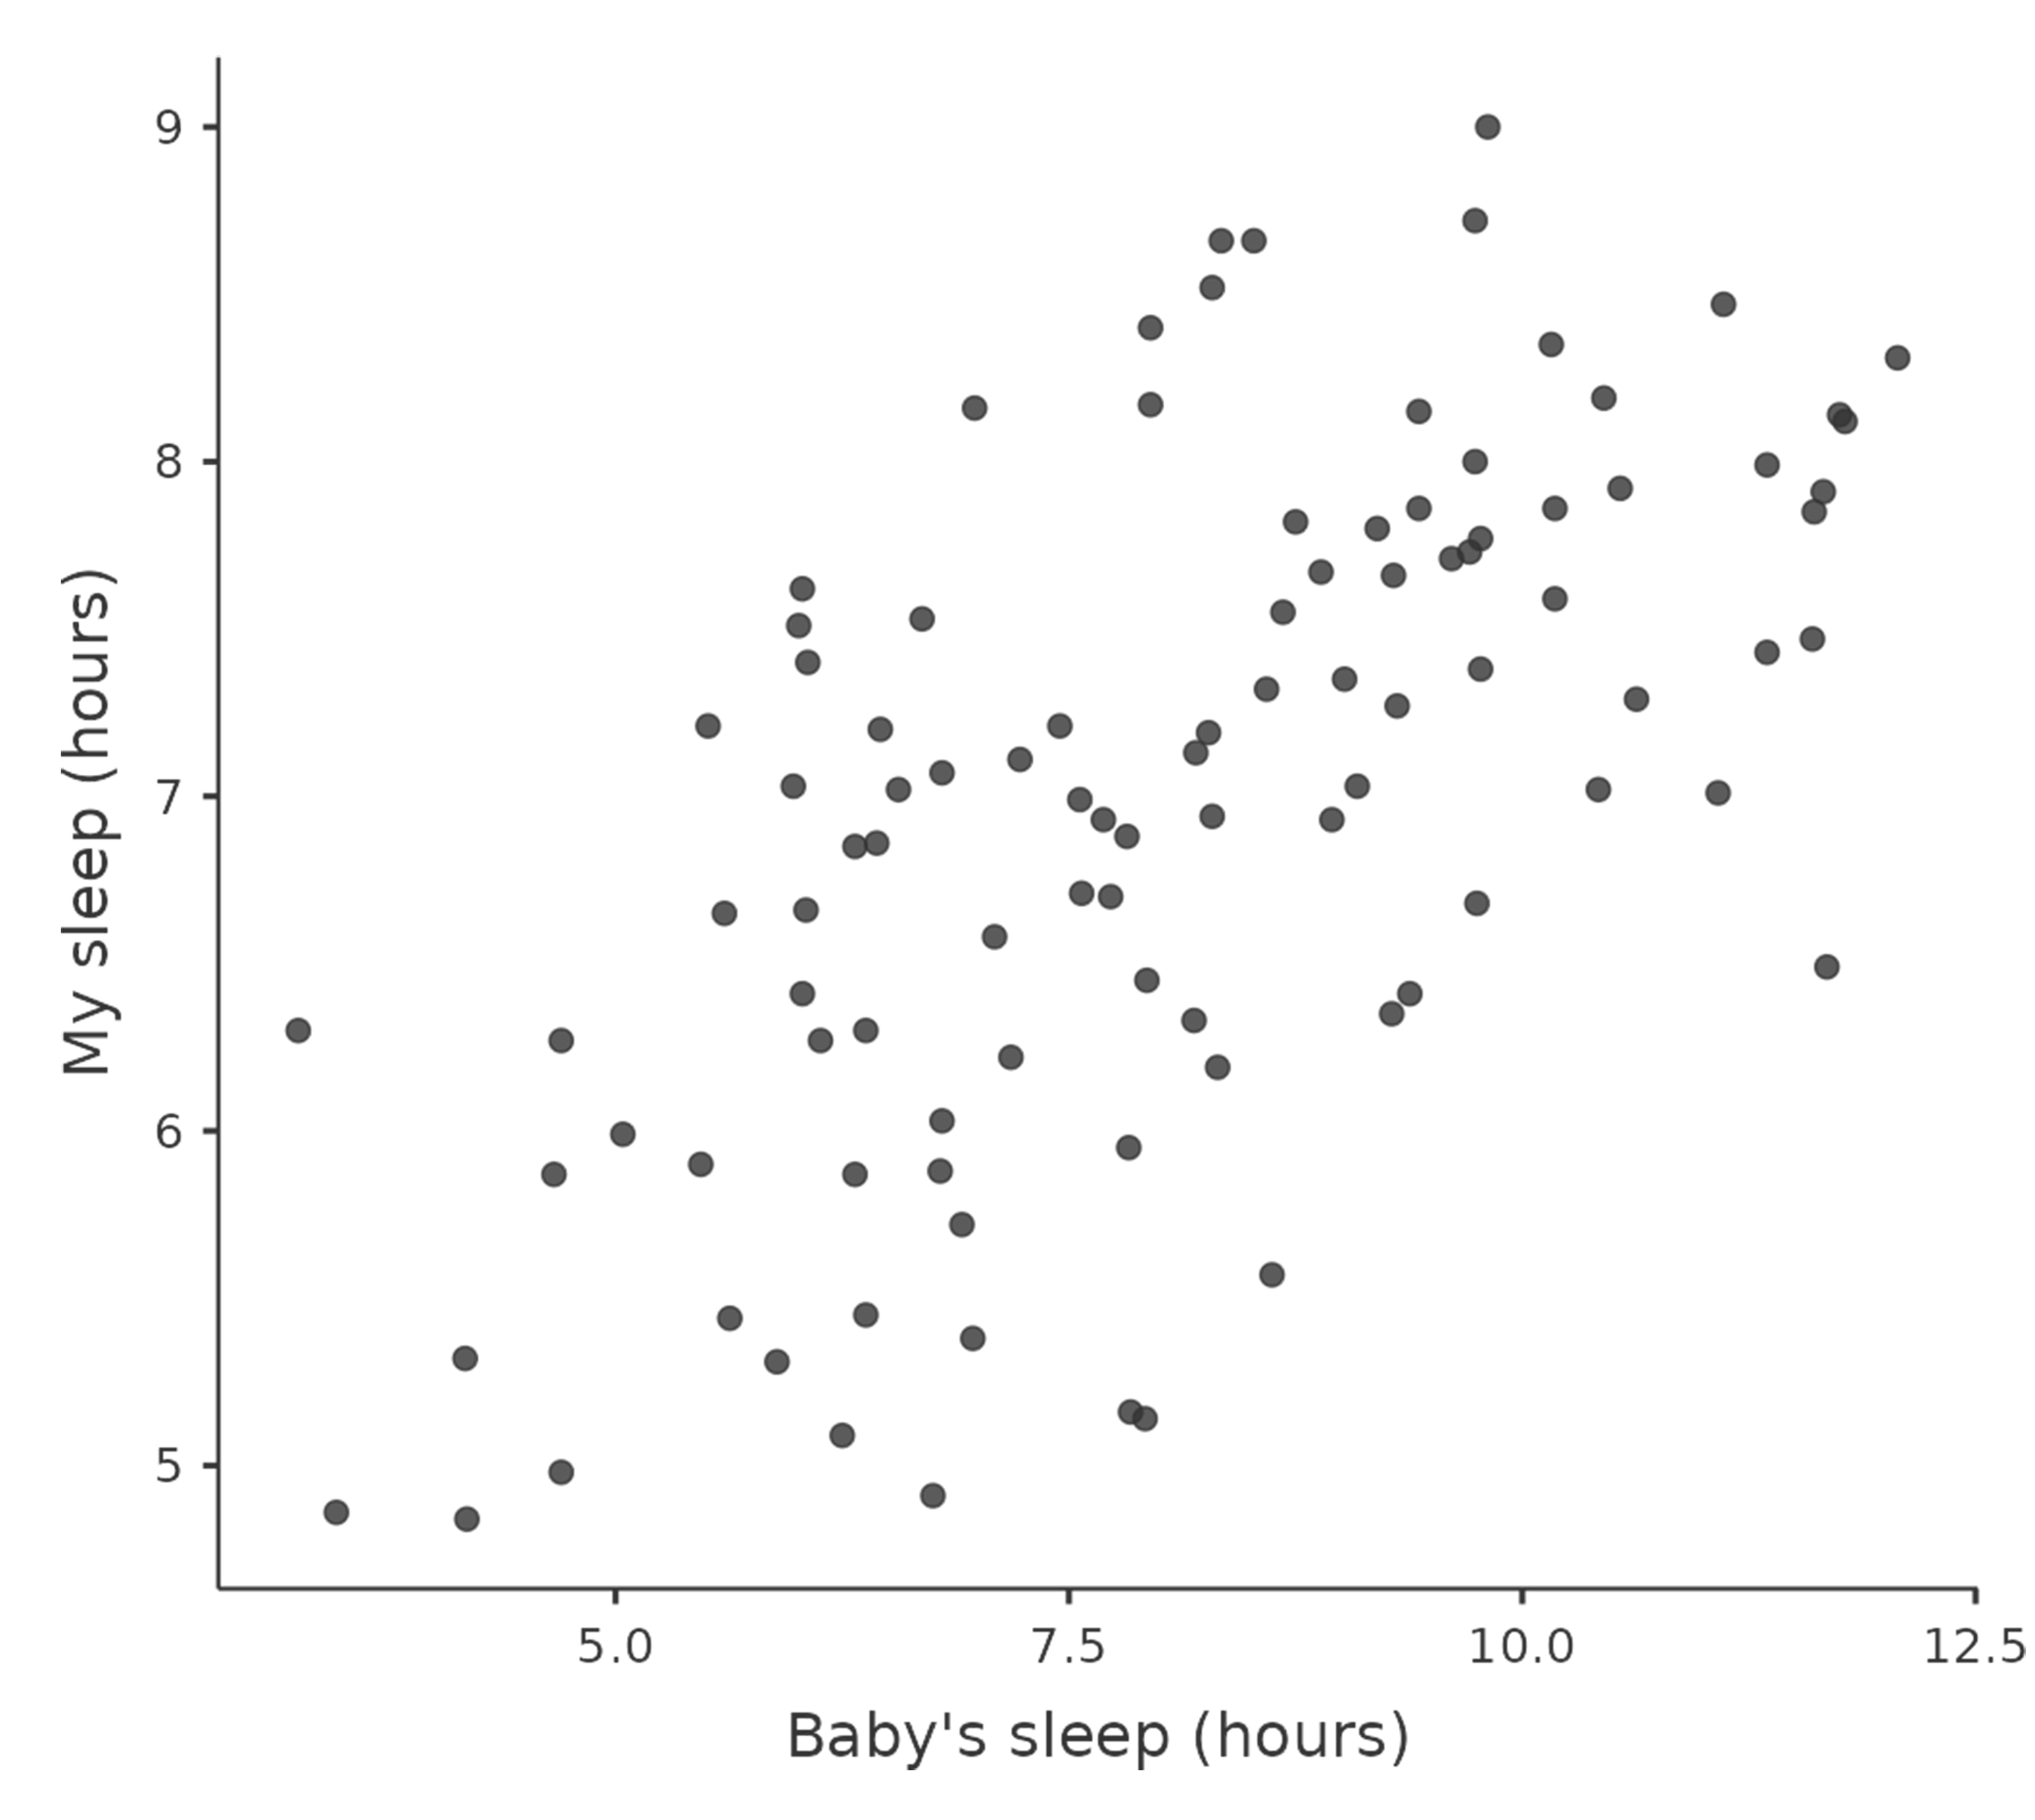
\includegraphics{images/fig12-3b.png}

}

\subcaption{\label{fig-fig12-3b}}
\end{minipage}%

\caption{\label{fig-fig12-3}Scatterplots from jamovi showing the
relationship between baby.sleep and dani.grump (left), as compared to
the relationship between baby.sleep and dani.sleep (right)}

\end{figure}

\hypertarget{the-correlation-coefficient}{%
\subsection{The correlation
coefficient}\label{the-correlation-coefficient}}

We can make these ideas a bit more explicit by introducing the idea of a
\textbf{correlation coefficient} (or, more specifically, Pearson's
correlation coefficient), which is traditionally denoted as r. The
correlation coefficient between two variables \(X\) and \(Y\) (sometimes
denoted \(r_{XY}\) ), which we'll define more precisely in the next
section, is a measure that varies from -1 to 1. When \(r = -1\) it means
that we have a perfect negative relationship, and when \(r = 1\) it
means we have a perfect positive relationship. When \(r = 0\), there's
no relationship at all. If you look at Figure~\ref{fig-fig12-4}, you can
see several plots showing what different correlations look like.

{[}Additional technical detail\footnote{The formula for the Pearson's
  correlation coefficient can be written in several different ways. I
  think the simplest way to write down the formula is to break it into
  two steps. Firstly, let's introduce the idea of a \textbf{covariance}.
  The covariance between two variables \(X\) and \(Y\) is a
  generalisation of the notion of the variance and is a mathematically
  simple way of describing the relationship between two variables that
  isn't terribly informative to humans
  \[Cov(X,Y)=\frac{1}{N-1}\sum_{i=1}^N(X_i-\bar{X})(Y_i-\bar{Y})\]
  Because we're multiplying (i.e., taking the ``product'' of) a quantity
  that depends on X by a quantity that depends on Y and then
  averaging,\(^a\) you can think of the formula for the covariance as an
  ``average cross product'' between \(X\) and \(Y\). The covariance has
  the nice property that, if \(X\) and \(Y\) are entirely unrelated,
  then the covariance is exactly zero. If the relationship between them
  is positive (in the sense shown in Figure~\ref{fig-fig12-4} then the
  covariance is also positive, and if the relationship is negative then
  the covariance is also negative. In other words, the covariance
  captures the basic qualitative idea of correlation. Unfortunately, the
  raw magnitude of the covariance isn't easy to interpret as it depends
  on the units in which \(X\) and \(Y\) are expressed and, worse yet,
  the actual units that the covariance itself is expressed in are really
  weird. For instance, if \(X\) refers to the dani.sleep variable
  (units: hours) and \(Y\) refers to the dani.grump variable (units:
  grumps), then the units for their covariance are
  \(hours \times grumps\). And I have no freaking idea what that would
  even mean. The Pearson correlation coefficient r fixes this
  interpretation problem by standardising the covariance, in pretty much
  the exact same way that the \emph{z}-score standardises a raw score,
  by dividing by the standard deviation. However, because we have two
  variables that contribute to the covariance, the standardisation only
  works if we divide by both standard deviations.\(^b\) In other words,
  the correlation between \(X\) and \(Y\) can be written as follows:
  \[r_{XY}=\frac{Cov(X,Y)}{\hat{\sigma}_X\hat{\sigma}_Y}\]---\(^a\) Just
  like we saw with the variance and the standard deviation, in practice
  we divide by \(N - 1\) rather than \(N\). \(^b\) This is an
  oversimplification, but it'll do for our purposes.}{]}

\begin{figure}

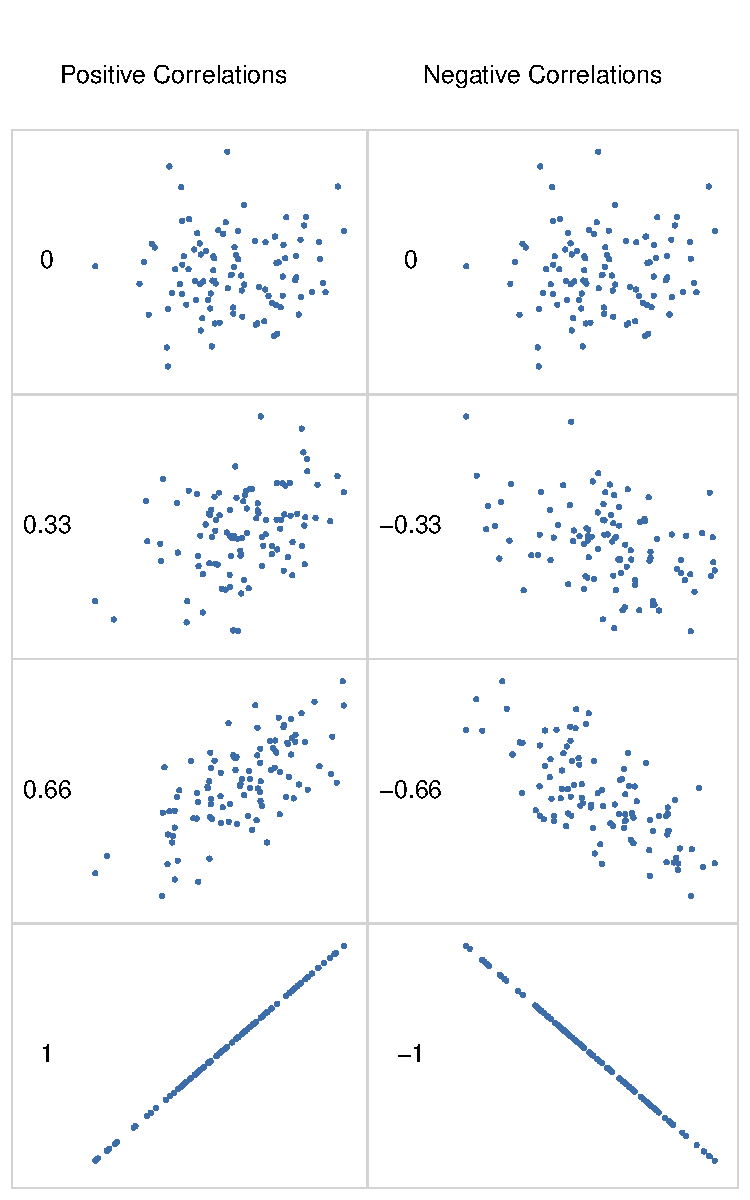
\includegraphics[width=1\textwidth,height=\textheight]{12-Correlation-and-linear-regression_files/figure-pdf/fig-fig12-4-1.pdf} \hfill{}

\caption{\label{fig-fig12-4}Illustration of the effect of varying the
strength and direction of a correlation. In the left-hand column, the
correlations are \(0, .33, .66\) and \(1\). In the right-hand column,
the correlations are \(0, -.33, -.66\) and \(-1\)}

\end{figure}

By standardising the covariance, not only do we keep all of the nice
properties of the covariance discussed earlier, but the actual values of
r are on a meaningful scale: r = 1 implies a perfect positive
relationship and \(r = -1\) implies a perfect negative relationship.
I'll expand a little more on this point later, in the section on
\protect\hyperlink{interpreting-a-correlation}{Interpreting a
correlation}. But before I do, let's look at how to calculate
correlations in jamovi.

\hypertarget{calculating-correlations-in-jamovi}{%
\subsection{Calculating correlations in
jamovi}\label{calculating-correlations-in-jamovi}}

Calculating correlations in jamovi can be done by clicking on the
`Regression' - `Correlation Matrix' button. Transfer all four continuous
variables across into the box on the right to get the output in
Figure~\ref{fig-fig12-5}.

\begin{figure}

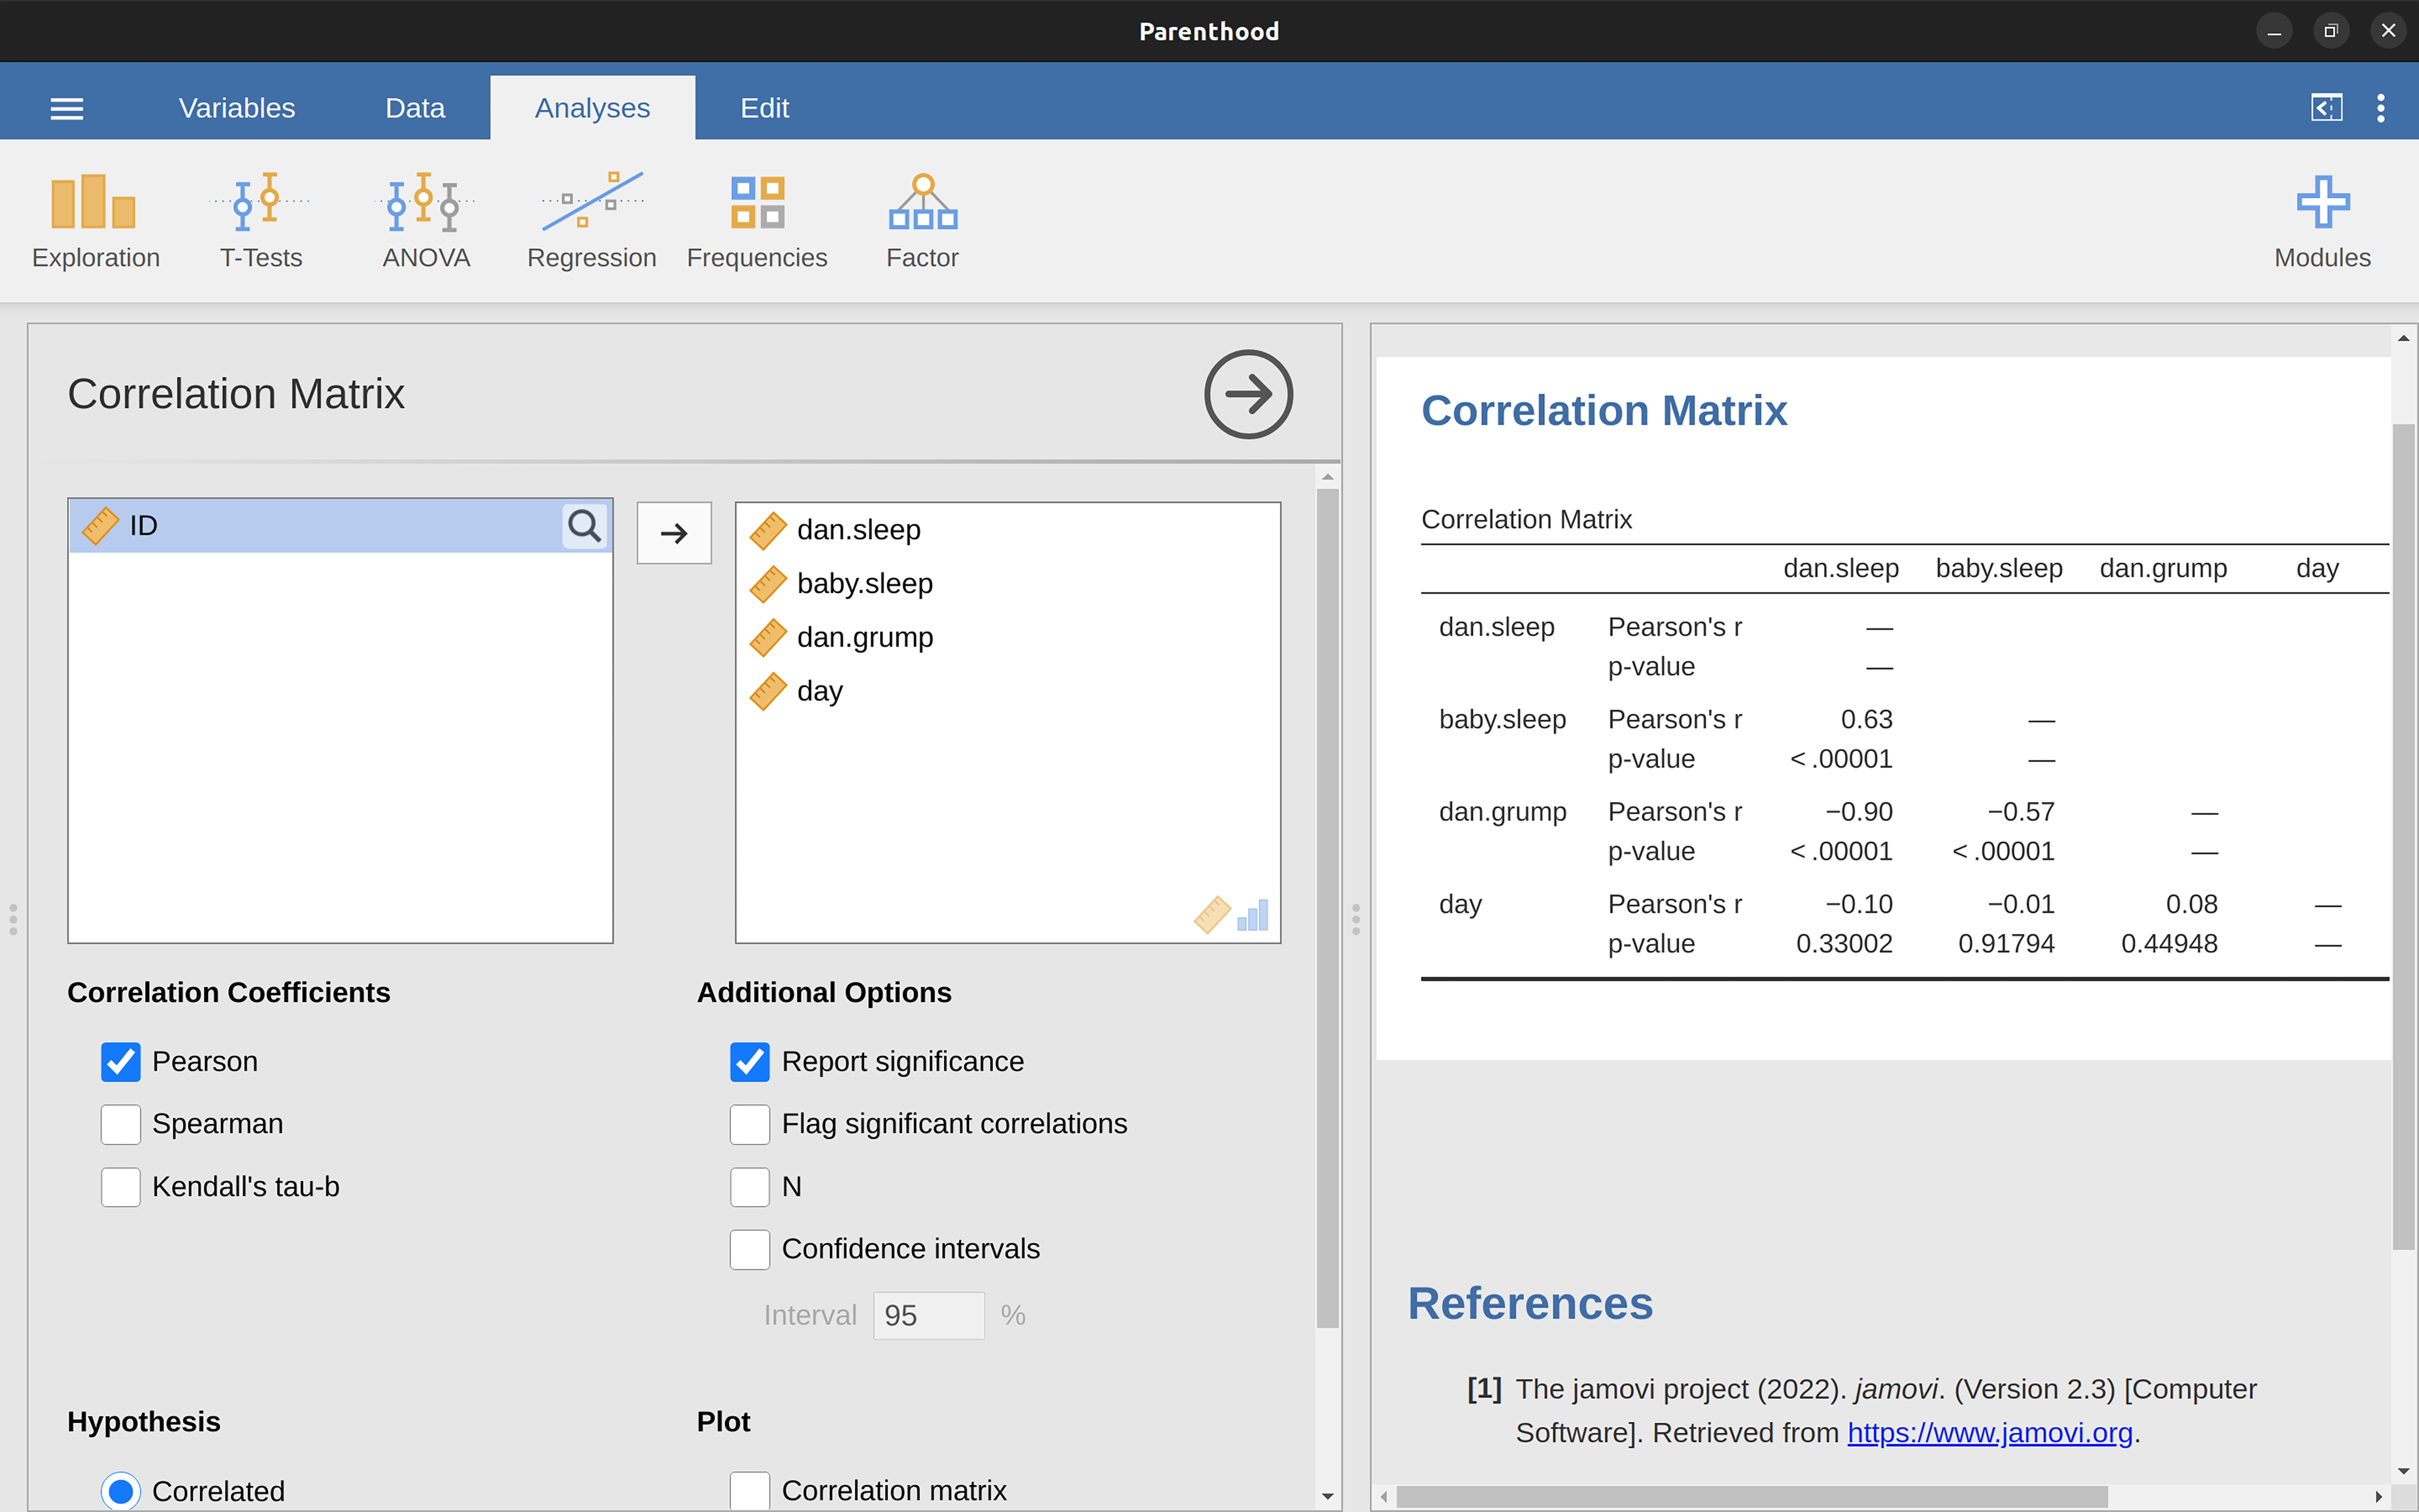
\includegraphics[width=1\textwidth,height=\textheight]{images/fig12-5.png} \hfill{}

\caption{\label{fig-fig12-5}A jamovi screenshot showing correlations
between variables in the \emph{parenthood.csv} file}

\end{figure}

\hypertarget{interpreting-a-correlation}{%
\subsection{Interpreting a
correlation}\label{interpreting-a-correlation}}

Naturally, in real life you don't see many correlations of \(1\). So how
should you interpret a correlation of, say, r = \(.4\)? The honest
answer is that it really depends on what you want to use the data for,
and on how strong the correlations in your field tend to be. A friend of
mine in engineering once argued that any correlation less than \(.95\)
is completely useless (I think he was exaggerating, even for
engineering). On the other hand, there are real cases, even in
psychology, where you should really expect correlations that strong. For
instance, one of the benchmark data sets used to test theories of how
people judge similarities is so clean that any theory that can't achieve
a correlation of at least \(.9\) really isn't deemed to be successful.
However, when looking for (say) elementary correlates of intelligence
(e.g., inspection time, response time), if you get a correlation above
\(.3\) you're doing very very well. In short, the interpretation of a
correlation depends a lot on the context. That said, the rough guide in
Table~\ref{tbl-tab12-2} is pretty typical.

\hypertarget{tbl-tab12-2}{}
 
  \providecommand{\huxb}[2]{\arrayrulecolor[RGB]{#1}\global\arrayrulewidth=#2pt}
  \providecommand{\huxvb}[2]{\color[RGB]{#1}\vrule width #2pt}
  \providecommand{\huxtpad}[1]{\rule{0pt}{#1}}
  \providecommand{\huxbpad}[1]{\rule[-#1]{0pt}{#1}}

\begin{table}[ht]
\caption{\label{tbl-tab12-2}A rough guide to interpreting correlations }\tabularnewline

\begin{centerbox}
\begin{threeparttable}
\setlength{\tabcolsep}{0pt}
\begin{tabularx}{0.9\textwidth}{p{0.3\textwidth} p{0.3\textwidth} p{0.3\textwidth}}


\hhline{>{\huxb{0, 0, 0}{0.4}}->{\huxb{0, 0, 0}{0.4}}->{\huxb{0, 0, 0}{0.4}}-}
\arrayrulecolor{black}

\multicolumn{1}{!{\huxvb{0, 0, 0}{0}}p{0.3\textwidth}!{\huxvb{0, 0, 0}{0}}}{\hspace{0pt}\parbox[b]{0.3\textwidth-0pt-12pt}{\huxtpad{2pt + 1em}\centering \textbf{Correlation}\huxbpad{2pt}}} &
\multicolumn{1}{p{0.3\textwidth}!{\huxvb{0, 0, 0}{0}}}{\hspace{12pt}\parbox[b]{0.3\textwidth-12pt-12pt}{\huxtpad{2pt + 1em}\centering \textbf{Strength}\huxbpad{2pt}}} &
\multicolumn{1}{p{0.3\textwidth}!{\huxvb{0, 0, 0}{0}}}{\hspace{12pt}\parbox[b]{0.3\textwidth-12pt-0pt}{\huxtpad{2pt + 1em}\centering \textbf{Direction}\huxbpad{2pt}}} \tabularnewline[-0.5pt]


\hhline{>{\huxb{0, 0, 0}{0.4}}->{\huxb{0, 0, 0}{0.4}}->{\huxb{0, 0, 0}{0.4}}-}
\arrayrulecolor{black}

\multicolumn{1}{!{\huxvb{0, 0, 0}{0}}p{0.3\textwidth}!{\huxvb{0, 0, 0}{0}}}{\hspace{0pt}\parbox[b]{0.3\textwidth-0pt-12pt}{\huxtpad{2pt + 1em}\centering -1.00 to -0.90\huxbpad{2pt}}} &
\multicolumn{1}{p{0.3\textwidth}!{\huxvb{0, 0, 0}{0}}}{\hspace{12pt}\parbox[b]{0.3\textwidth-12pt-12pt}{\huxtpad{2pt + 1em}\centering Very strong\huxbpad{2pt}}} &
\multicolumn{1}{p{0.3\textwidth}!{\huxvb{0, 0, 0}{0}}}{\hspace{12pt}\parbox[b]{0.3\textwidth-12pt-0pt}{\huxtpad{2pt + 1em}\centering Negative\huxbpad{2pt}}} \tabularnewline[-0.5pt]


\hhline{}
\arrayrulecolor{black}

\multicolumn{1}{!{\huxvb{0, 0, 0}{0}}p{0.3\textwidth}!{\huxvb{0, 0, 0}{0}}}{\hspace{0pt}\parbox[b]{0.3\textwidth-0pt-12pt}{\huxtpad{2pt + 1em}\centering -0.90 to -0.70\huxbpad{2pt}}} &
\multicolumn{1}{p{0.3\textwidth}!{\huxvb{0, 0, 0}{0}}}{\hspace{12pt}\parbox[b]{0.3\textwidth-12pt-12pt}{\huxtpad{2pt + 1em}\centering Strong\huxbpad{2pt}}} &
\multicolumn{1}{p{0.3\textwidth}!{\huxvb{0, 0, 0}{0}}}{\hspace{12pt}\parbox[b]{0.3\textwidth-12pt-0pt}{\huxtpad{2pt + 1em}\centering Negative\huxbpad{2pt}}} \tabularnewline[-0.5pt]


\hhline{}
\arrayrulecolor{black}

\multicolumn{1}{!{\huxvb{0, 0, 0}{0}}p{0.3\textwidth}!{\huxvb{0, 0, 0}{0}}}{\hspace{0pt}\parbox[b]{0.3\textwidth-0pt-12pt}{\huxtpad{2pt + 1em}\centering -0.70 to -0.40\huxbpad{2pt}}} &
\multicolumn{1}{p{0.3\textwidth}!{\huxvb{0, 0, 0}{0}}}{\hspace{12pt}\parbox[b]{0.3\textwidth-12pt-12pt}{\huxtpad{2pt + 1em}\centering Moderate\huxbpad{2pt}}} &
\multicolumn{1}{p{0.3\textwidth}!{\huxvb{0, 0, 0}{0}}}{\hspace{12pt}\parbox[b]{0.3\textwidth-12pt-0pt}{\huxtpad{2pt + 1em}\centering Negative\huxbpad{2pt}}} \tabularnewline[-0.5pt]


\hhline{}
\arrayrulecolor{black}

\multicolumn{1}{!{\huxvb{0, 0, 0}{0}}p{0.3\textwidth}!{\huxvb{0, 0, 0}{0}}}{\hspace{0pt}\parbox[b]{0.3\textwidth-0pt-12pt}{\huxtpad{2pt + 1em}\centering -0.40 to -0.20\huxbpad{2pt}}} &
\multicolumn{1}{p{0.3\textwidth}!{\huxvb{0, 0, 0}{0}}}{\hspace{12pt}\parbox[b]{0.3\textwidth-12pt-12pt}{\huxtpad{2pt + 1em}\centering Weak\huxbpad{2pt}}} &
\multicolumn{1}{p{0.3\textwidth}!{\huxvb{0, 0, 0}{0}}}{\hspace{12pt}\parbox[b]{0.3\textwidth-12pt-0pt}{\huxtpad{2pt + 1em}\centering Negative\huxbpad{2pt}}} \tabularnewline[-0.5pt]


\hhline{}
\arrayrulecolor{black}

\multicolumn{1}{!{\huxvb{0, 0, 0}{0}}p{0.3\textwidth}!{\huxvb{0, 0, 0}{0}}}{\hspace{0pt}\parbox[b]{0.3\textwidth-0pt-12pt}{\huxtpad{2pt + 1em}\centering -0.20 to 0.00\huxbpad{2pt}}} &
\multicolumn{1}{p{0.3\textwidth}!{\huxvb{0, 0, 0}{0}}}{\hspace{12pt}\parbox[b]{0.3\textwidth-12pt-12pt}{\huxtpad{2pt + 1em}\centering Negligible\huxbpad{2pt}}} &
\multicolumn{1}{p{0.3\textwidth}!{\huxvb{0, 0, 0}{0}}}{\hspace{12pt}\parbox[b]{0.3\textwidth-12pt-0pt}{\huxtpad{2pt + 1em}\centering Negative\huxbpad{2pt}}} \tabularnewline[-0.5pt]


\hhline{}
\arrayrulecolor{black}

\multicolumn{1}{!{\huxvb{0, 0, 0}{0}}p{0.3\textwidth}!{\huxvb{0, 0, 0}{0}}}{\hspace{0pt}\parbox[b]{0.3\textwidth-0pt-12pt}{\huxtpad{2pt + 1em}\centering 0.00 to 0.20\huxbpad{2pt}}} &
\multicolumn{1}{p{0.3\textwidth}!{\huxvb{0, 0, 0}{0}}}{\hspace{12pt}\parbox[b]{0.3\textwidth-12pt-12pt}{\huxtpad{2pt + 1em}\centering Negligible\huxbpad{2pt}}} &
\multicolumn{1}{p{0.3\textwidth}!{\huxvb{0, 0, 0}{0}}}{\hspace{12pt}\parbox[b]{0.3\textwidth-12pt-0pt}{\huxtpad{2pt + 1em}\centering Positive\huxbpad{2pt}}} \tabularnewline[-0.5pt]


\hhline{}
\arrayrulecolor{black}

\multicolumn{1}{!{\huxvb{0, 0, 0}{0}}p{0.3\textwidth}!{\huxvb{0, 0, 0}{0}}}{\hspace{0pt}\parbox[b]{0.3\textwidth-0pt-12pt}{\huxtpad{2pt + 1em}\centering 0.20 to 0.40\huxbpad{2pt}}} &
\multicolumn{1}{p{0.3\textwidth}!{\huxvb{0, 0, 0}{0}}}{\hspace{12pt}\parbox[b]{0.3\textwidth-12pt-12pt}{\huxtpad{2pt + 1em}\centering Weak\huxbpad{2pt}}} &
\multicolumn{1}{p{0.3\textwidth}!{\huxvb{0, 0, 0}{0}}}{\hspace{12pt}\parbox[b]{0.3\textwidth-12pt-0pt}{\huxtpad{2pt + 1em}\centering Positive\huxbpad{2pt}}} \tabularnewline[-0.5pt]


\hhline{}
\arrayrulecolor{black}

\multicolumn{1}{!{\huxvb{0, 0, 0}{0}}p{0.3\textwidth}!{\huxvb{0, 0, 0}{0}}}{\hspace{0pt}\parbox[b]{0.3\textwidth-0pt-12pt}{\huxtpad{2pt + 1em}\centering 0.40 to 0.70\huxbpad{2pt}}} &
\multicolumn{1}{p{0.3\textwidth}!{\huxvb{0, 0, 0}{0}}}{\hspace{12pt}\parbox[b]{0.3\textwidth-12pt-12pt}{\huxtpad{2pt + 1em}\centering Moderate\huxbpad{2pt}}} &
\multicolumn{1}{p{0.3\textwidth}!{\huxvb{0, 0, 0}{0}}}{\hspace{12pt}\parbox[b]{0.3\textwidth-12pt-0pt}{\huxtpad{2pt + 1em}\centering Positive\huxbpad{2pt}}} \tabularnewline[-0.5pt]


\hhline{}
\arrayrulecolor{black}

\multicolumn{1}{!{\huxvb{0, 0, 0}{0}}p{0.3\textwidth}!{\huxvb{0, 0, 0}{0}}}{\hspace{0pt}\parbox[b]{0.3\textwidth-0pt-12pt}{\huxtpad{2pt + 1em}\centering {\fontsize{10pt}{12pt}\selectfont 0.70 to 0.90}\huxbpad{2pt}}} &
\multicolumn{1}{p{0.3\textwidth}!{\huxvb{0, 0, 0}{0}}}{\hspace{12pt}\parbox[b]{0.3\textwidth-12pt-12pt}{\huxtpad{2pt + 1em}\centering {\fontsize{10pt}{12pt}\selectfont Strong}\huxbpad{2pt}}} &
\multicolumn{1}{p{0.3\textwidth}!{\huxvb{0, 0, 0}{0}}}{\hspace{12pt}\parbox[b]{0.3\textwidth-12pt-0pt}{\huxtpad{2pt + 1em}\centering {\fontsize{10pt}{12pt}\selectfont Positive}\huxbpad{2pt}}} \tabularnewline[-0.5pt]


\hhline{}
\arrayrulecolor{black}

\multicolumn{1}{!{\huxvb{0, 0, 0}{0}}p{0.3\textwidth}!{\huxvb{0, 0, 0}{0}}}{\hspace{0pt}\parbox[b]{0.3\textwidth-0pt-12pt}{\huxtpad{2pt + 1em}\centering 0.90 to 1.00\huxbpad{2pt}}} &
\multicolumn{1}{p{0.3\textwidth}!{\huxvb{0, 0, 0}{0}}}{\hspace{12pt}\parbox[b]{0.3\textwidth-12pt-12pt}{\huxtpad{2pt + 1em}\centering Very strong\huxbpad{2pt}}} &
\multicolumn{1}{p{0.3\textwidth}!{\huxvb{0, 0, 0}{0}}}{\hspace{12pt}\parbox[b]{0.3\textwidth-12pt-0pt}{\huxtpad{2pt + 1em}\centering Positive\huxbpad{2pt}}} \tabularnewline[-0.5pt]


\hhline{>{\huxb{0, 0, 0}{0.8}}->{\huxb{0, 0, 0}{0.8}}->{\huxb{0, 0, 0}{0.8}}-}
\arrayrulecolor{black}

\multicolumn{3}{!{\huxvb{0, 0, 0}{0}}p{0.9\textwidth+4\tabcolsep}!{\huxvb{0, 0, 0}{0}}}{\hspace{6pt}\parbox[b]{0.9\textwidth+4\tabcolsep-6pt-6pt}{\huxtpad{6pt + 1em}\raggedright \textit{*Note that I say a rough guide. There aren't hard and fast rules for what counts as strong or weak relationships. It depends on the context}\huxbpad{6pt}}} \tabularnewline[-0.5pt]


\hhline{}
\arrayrulecolor{black}
\end{tabularx} 

\end{threeparttable}\par\end{centerbox}

\end{table}
 

However, something that can never be stressed enough is that you should
always look at the scatterplot before attaching any interpretation to
the data. A correlation might not mean what you think it means. The
classic illustration of this is ``Anscombe's Quartet'' (Anscombe, 1973),
a collection of four data sets. Each data set has two variables, an
\(X\) and a \(Y\). For all four data sets the mean value for \(X\) is
\(9\) and the mean for \(Y\) is \(7.5\). The standard deviations for all
\(X\) variables are almost identical, as are those for the Y variables.
And in each case the correlation between \(X\) and \(Y\) is
\(r = 0.816\). You can verify this yourself, since I happen to have
saved it in a file called \emph{anscombe.csv}.

You'd think that these four data sets would look pretty similar to one
another. They do not. If we draw scatterplots of \(X\) against \(Y\) for
all four variables, as shown in Figure~\ref{fig-fig12-6}, we see that
all four of these are spectacularly different to each other. The lesson
here, which so very many people seem to forget in real life, is ``always
graph your raw data'' (see \textbf{?@sec-Drawing-graphs}).

\begin{figure}

\begin{minipage}[t]{\linewidth}

{\centering 


\includegraphics[width=0.45\textwidth,height=\textheight]{images/fig12-6a.png}

\includegraphics[width=0.45\textwidth,height=\textheight]{images/fig12-6b.png}

\includegraphics[width=0.45\textwidth,height=\textheight]{images/fig12-6c.png}

\includegraphics[width=0.45\textwidth,height=\textheight]{images/fig12-6d.png}

}

\end{minipage}%

\caption{\label{fig-fig12-6}Anscombe's quartet scatterplots in jamovi.
All four of these data sets have a Pearson correlation of \(r\) = .816,
but they are qualitatively different from one another}

\end{figure}

\hypertarget{spearmans-rank-correlations}{%
\subsection{Spearman's rank
correlations}\label{spearmans-rank-correlations}}

The Pearson correlation coefficient is useful for a lot of things, but
it does have shortcomings. One issue in particular stands out: what it
actually measures is the strength of the linear relationship between two
variables. In other words, what it gives you is a measure of the extent
to which the data all tend to fall on a single, perfectly straight line.
Often, this is a pretty good approximation to what we mean when we say
``relationship'', and so the Pearson correlation is a good thing to
calculate. Sometimes though, it isn't.

One very common situation where the Pearson correlation isn't quite the
right thing to use arises when an increase in one variable \(X\) really
is reflected in an increase in another variable Y , but the nature of
the relationship isn't necessarily linear. An example of this might be
the relationship between effort and reward when studying for an exam. If
you put zero effort (\(X\)) into learning a subject then you should
expect a grade of \(0\%\) (\(Y\)). However, a little bit of effort will
cause a massive improvement. Just turning up to lectures means that you
learn a fair bit, and if you just turn up to classes and scribble a few
things down your grade might rise to 35\%, all without a lot of effort.
However, you just don't get the same effect at the other end of the
scale. As everyone knows, it takes a lot more effort to get a grade of
\(90\%\) than it takes to get a grade of \(55\%\). What this means is
that, if I've got data looking at study effort and grades, there's a
pretty good chance that Pearson correlations will be misleading.

To illustrate, consider the data plotted in Figure~\ref{fig-fig12-7},
showing the relationship between hours worked and grade received for 10
students taking some class. The curious thing about this (highly
fictitious) data set is that increasing your effort always increases
your grade. It might be by a lot or it might be by a little, but
increasing effort will never decrease your grade. If we run a standard
Pearson correlation, it shows a strong relationship between hours worked
and grade received, with a correlation coefficient of \(0.91\). However,
this doesn't actually capture the observation that increasing hours
worked always increases the grade. There's a sense here in which we want
to be able to say that the correlation is perfect but for a somewhat
different notion of what a ``relationship'' is. What we're looking for
is something that captures the fact that there is a perfect
\textbf{ordinal relationship} here. That is, if student 1 works more
hours than student 2, then we can guarantee that student 1 will get the
better grade. That's not what a correlation of \(r = .91\) says at all.

\begin{figure}

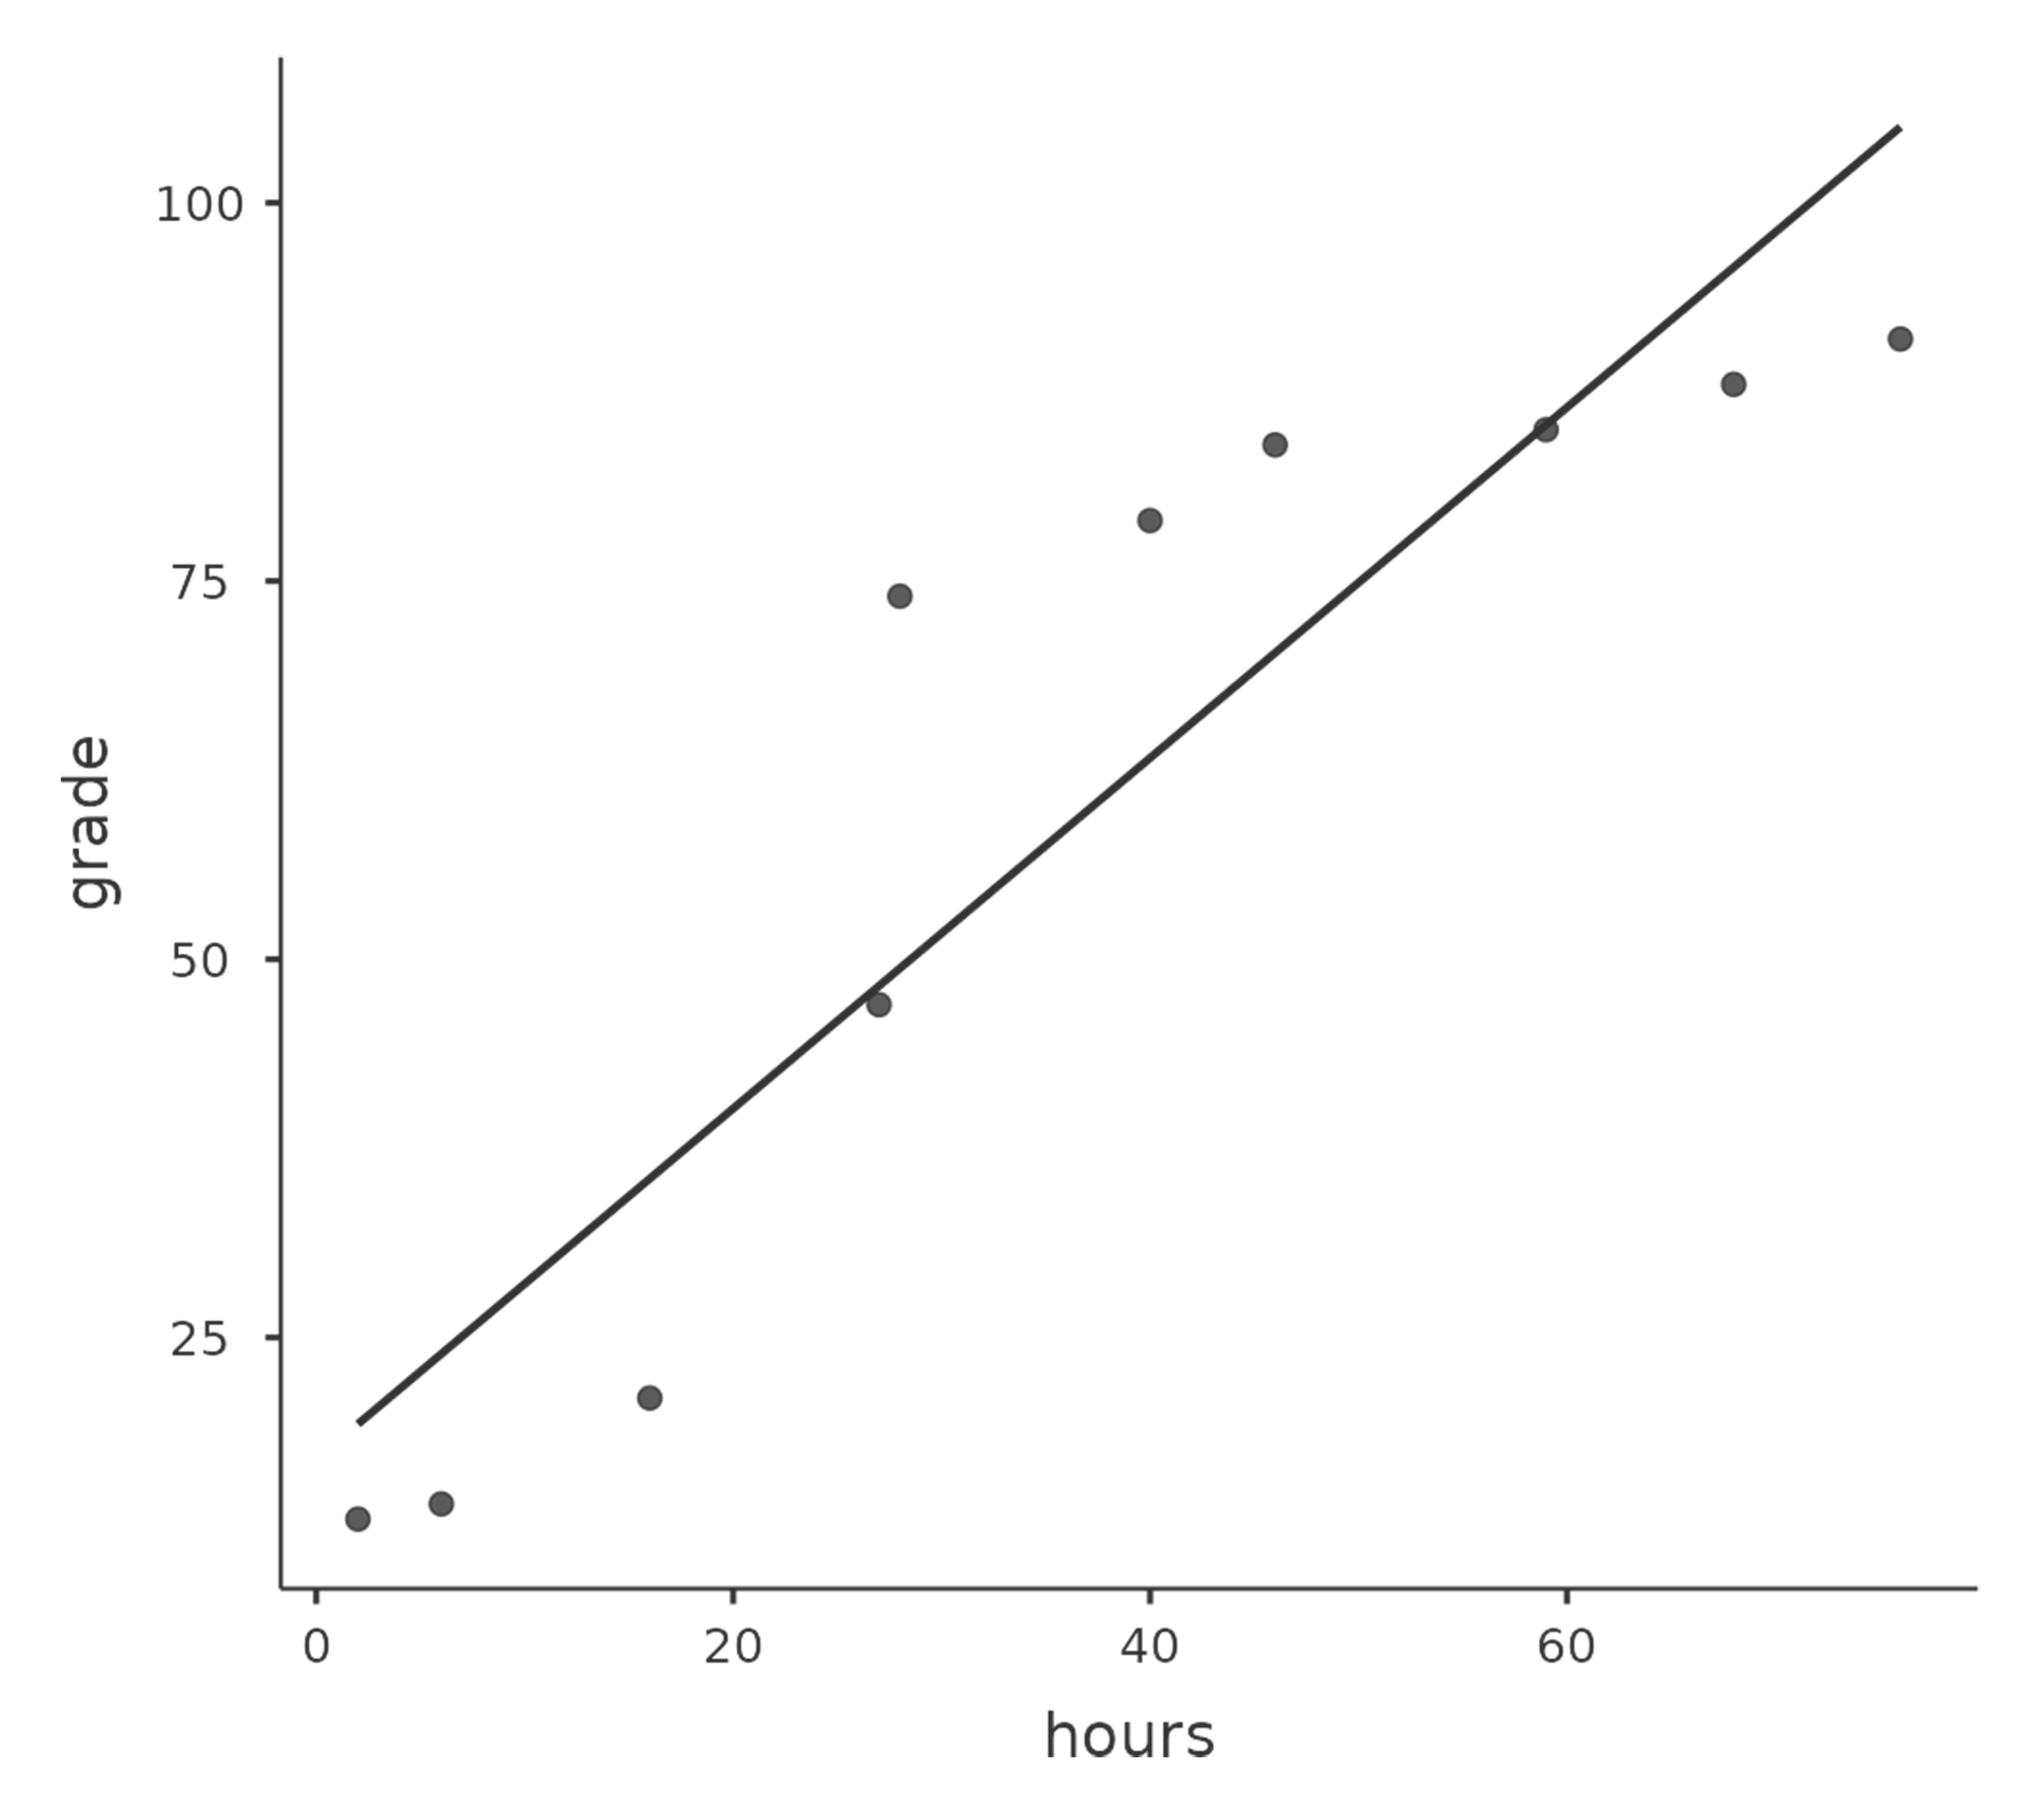
\includegraphics[width=1\textwidth,height=\textheight]{images/fig12-7.png} \hfill{}

\caption{\label{fig-fig12-7}The relationship between hours worked and
grade received for a toy data set consisting of only 10 students (each
dot corresponds to one student). The line through the middle shows the
linear relationship between the two variables. This produces a strong
Pearson correlation of \(r = .91\). However, the interesting thing to
note here is that there's actually a perfect monotonic relationship
between the two variables. In this toy example, increasing the hours
worked always increases the grade received, as illustrated by the solid
line. This is reflected in a Spearman correlation of \(\rho = 1\). With
such a small data set, however, it's an open question as to which
version better describes the actual relationship involved}

\end{figure}

How should we address this? Actually, it's really easy. If we're looking
for ordinal relationships all we have to do is treat the data as if it
were ordinal scale! So, instead of measuring effort in terms of ``hours
worked'', lets rank all \(10\) of our students in order of hours worked.
That is, student \(1\) did the least work out of anyone (\(2\) hours) so
they get the lowest rank (rank = \(1\)). Student \(4\) was the next
laziest, putting in only \(6\) hours of work over the whole semester, so
they get the next lowest rank (rank = \(2\)). Notice that I'm using
``rank =1'' to mean ``low rank''. Sometimes in everyday language we talk
about ``rank = \(1\)'' to mean ``top rank'' rather than ``bottom rank''.
So be careful, you can rank ``from smallest value to largest value''
(i.e., small equals rank \(1\)) or you can rank ``from largest value to
smallest value'' (i.e., large equals rank 1). In this case, I'm ranking
from smallest to largest, but as it's really easy to forget which way
you set things up you have to put a bit of effort into remembering!

Okay, so let's have a look at our students when we rank them from worst
to best in terms of effort and reward Table~\ref{tbl-tab12-3}.

\hypertarget{tbl-tab12-3}{}
 
  \providecommand{\huxb}[2]{\arrayrulecolor[RGB]{#1}\global\arrayrulewidth=#2pt}
  \providecommand{\huxvb}[2]{\color[RGB]{#1}\vrule width #2pt}
  \providecommand{\huxtpad}[1]{\rule{0pt}{#1}}
  \providecommand{\huxbpad}[1]{\rule[-#1]{0pt}{#1}}

\begin{table}[ht]
\caption{\label{tbl-tab12-3}Students ranked in terms of effort and reward }\tabularnewline

\begin{centerbox}
\begin{threeparttable}
\setlength{\tabcolsep}{0pt}
\begin{tabularx}{0.9\textwidth}{p{0.3\textwidth} p{0.3\textwidth} p{0.3\textwidth}}


\hhline{>{\huxb{0, 0, 0}{0.4}}->{\huxb{0, 0, 0}{0.4}}->{\huxb{0, 0, 0}{0.4}}-}
\arrayrulecolor{black}

\multicolumn{1}{!{\huxvb{0, 0, 0}{0}}p{0.3\textwidth}!{\huxvb{0, 0, 0}{0}}}{\hspace{0pt}\parbox[b]{0.3\textwidth-0pt-12pt}{\huxtpad{2pt + 1em}\centering \textbf{}\huxbpad{2pt}}} &
\multicolumn{1}{p{0.3\textwidth}!{\huxvb{0, 0, 0}{0}}}{\hspace{12pt}\parbox[b]{0.3\textwidth-12pt-12pt}{\huxtpad{2pt + 1em}\centering \textbf{rank (hours worked)}\huxbpad{2pt}}} &
\multicolumn{1}{p{0.3\textwidth}!{\huxvb{0, 0, 0}{0}}}{\hspace{12pt}\parbox[b]{0.3\textwidth-12pt-0pt}{\huxtpad{2pt + 1em}\centering \textbf{rank (grade received)}\huxbpad{2pt}}} \tabularnewline[-0.5pt]


\hhline{>{\huxb{0, 0, 0}{0.4}}->{\huxb{0, 0, 0}{0.4}}->{\huxb{0, 0, 0}{0.4}}-}
\arrayrulecolor{black}

\multicolumn{1}{!{\huxvb{0, 0, 0}{0}}p{0.3\textwidth}!{\huxvb{0, 0, 0}{0}}}{\hspace{0pt}\parbox[b]{0.3\textwidth-0pt-12pt}{\huxtpad{2pt + 1em}\centering student 1\huxbpad{2pt}}} &
\multicolumn{1}{p{0.3\textwidth}!{\huxvb{0, 0, 0}{0}}}{\hspace{12pt}\parbox[b]{0.3\textwidth-12pt-12pt}{\huxtpad{2pt + 1em}\centering 1\huxbpad{2pt}}} &
\multicolumn{1}{p{0.3\textwidth}!{\huxvb{0, 0, 0}{0}}}{\hspace{12pt}\parbox[b]{0.3\textwidth-12pt-0pt}{\huxtpad{2pt + 1em}\centering 1\huxbpad{2pt}}} \tabularnewline[-0.5pt]


\hhline{}
\arrayrulecolor{black}

\multicolumn{1}{!{\huxvb{0, 0, 0}{0}}p{0.3\textwidth}!{\huxvb{0, 0, 0}{0}}}{\hspace{0pt}\parbox[b]{0.3\textwidth-0pt-12pt}{\huxtpad{2pt + 1em}\centering student 2\huxbpad{2pt}}} &
\multicolumn{1}{p{0.3\textwidth}!{\huxvb{0, 0, 0}{0}}}{\hspace{12pt}\parbox[b]{0.3\textwidth-12pt-12pt}{\huxtpad{2pt + 1em}\centering 10\huxbpad{2pt}}} &
\multicolumn{1}{p{0.3\textwidth}!{\huxvb{0, 0, 0}{0}}}{\hspace{12pt}\parbox[b]{0.3\textwidth-12pt-0pt}{\huxtpad{2pt + 1em}\centering 10\huxbpad{2pt}}} \tabularnewline[-0.5pt]


\hhline{}
\arrayrulecolor{black}

\multicolumn{1}{!{\huxvb{0, 0, 0}{0}}p{0.3\textwidth}!{\huxvb{0, 0, 0}{0}}}{\hspace{0pt}\parbox[b]{0.3\textwidth-0pt-12pt}{\huxtpad{2pt + 1em}\centering student 3\huxbpad{2pt}}} &
\multicolumn{1}{p{0.3\textwidth}!{\huxvb{0, 0, 0}{0}}}{\hspace{12pt}\parbox[b]{0.3\textwidth-12pt-12pt}{\huxtpad{2pt + 1em}\centering 6\huxbpad{2pt}}} &
\multicolumn{1}{p{0.3\textwidth}!{\huxvb{0, 0, 0}{0}}}{\hspace{12pt}\parbox[b]{0.3\textwidth-12pt-0pt}{\huxtpad{2pt + 1em}\centering 6\huxbpad{2pt}}} \tabularnewline[-0.5pt]


\hhline{}
\arrayrulecolor{black}

\multicolumn{1}{!{\huxvb{0, 0, 0}{0}}p{0.3\textwidth}!{\huxvb{0, 0, 0}{0}}}{\hspace{0pt}\parbox[b]{0.3\textwidth-0pt-12pt}{\huxtpad{2pt + 1em}\centering student 4\huxbpad{2pt}}} &
\multicolumn{1}{p{0.3\textwidth}!{\huxvb{0, 0, 0}{0}}}{\hspace{12pt}\parbox[b]{0.3\textwidth-12pt-12pt}{\huxtpad{2pt + 1em}\centering 2\huxbpad{2pt}}} &
\multicolumn{1}{p{0.3\textwidth}!{\huxvb{0, 0, 0}{0}}}{\hspace{12pt}\parbox[b]{0.3\textwidth-12pt-0pt}{\huxtpad{2pt + 1em}\centering 2\huxbpad{2pt}}} \tabularnewline[-0.5pt]


\hhline{}
\arrayrulecolor{black}

\multicolumn{1}{!{\huxvb{0, 0, 0}{0}}p{0.3\textwidth}!{\huxvb{0, 0, 0}{0}}}{\hspace{0pt}\parbox[b]{0.3\textwidth-0pt-12pt}{\huxtpad{2pt + 1em}\centering student 5\huxbpad{2pt}}} &
\multicolumn{1}{p{0.3\textwidth}!{\huxvb{0, 0, 0}{0}}}{\hspace{12pt}\parbox[b]{0.3\textwidth-12pt-12pt}{\huxtpad{2pt + 1em}\centering 3\huxbpad{2pt}}} &
\multicolumn{1}{p{0.3\textwidth}!{\huxvb{0, 0, 0}{0}}}{\hspace{12pt}\parbox[b]{0.3\textwidth-12pt-0pt}{\huxtpad{2pt + 1em}\centering 3\huxbpad{2pt}}} \tabularnewline[-0.5pt]


\hhline{}
\arrayrulecolor{black}

\multicolumn{1}{!{\huxvb{0, 0, 0}{0}}p{0.3\textwidth}!{\huxvb{0, 0, 0}{0}}}{\hspace{0pt}\parbox[b]{0.3\textwidth-0pt-12pt}{\huxtpad{2pt + 1em}\centering student 6\huxbpad{2pt}}} &
\multicolumn{1}{p{0.3\textwidth}!{\huxvb{0, 0, 0}{0}}}{\hspace{12pt}\parbox[b]{0.3\textwidth-12pt-12pt}{\huxtpad{2pt + 1em}\centering 5\huxbpad{2pt}}} &
\multicolumn{1}{p{0.3\textwidth}!{\huxvb{0, 0, 0}{0}}}{\hspace{12pt}\parbox[b]{0.3\textwidth-12pt-0pt}{\huxtpad{2pt + 1em}\centering 5\huxbpad{2pt}}} \tabularnewline[-0.5pt]


\hhline{}
\arrayrulecolor{black}

\multicolumn{1}{!{\huxvb{0, 0, 0}{0}}p{0.3\textwidth}!{\huxvb{0, 0, 0}{0}}}{\hspace{0pt}\parbox[b]{0.3\textwidth-0pt-12pt}{\huxtpad{2pt + 1em}\centering student 7\huxbpad{2pt}}} &
\multicolumn{1}{p{0.3\textwidth}!{\huxvb{0, 0, 0}{0}}}{\hspace{12pt}\parbox[b]{0.3\textwidth-12pt-12pt}{\huxtpad{2pt + 1em}\centering 4\huxbpad{2pt}}} &
\multicolumn{1}{p{0.3\textwidth}!{\huxvb{0, 0, 0}{0}}}{\hspace{12pt}\parbox[b]{0.3\textwidth-12pt-0pt}{\huxtpad{2pt + 1em}\centering 4\huxbpad{2pt}}} \tabularnewline[-0.5pt]


\hhline{}
\arrayrulecolor{black}

\multicolumn{1}{!{\huxvb{0, 0, 0}{0}}p{0.3\textwidth}!{\huxvb{0, 0, 0}{0}}}{\hspace{0pt}\parbox[b]{0.3\textwidth-0pt-12pt}{\huxtpad{2pt + 1em}\centering student 8\huxbpad{2pt}}} &
\multicolumn{1}{p{0.3\textwidth}!{\huxvb{0, 0, 0}{0}}}{\hspace{12pt}\parbox[b]{0.3\textwidth-12pt-12pt}{\huxtpad{2pt + 1em}\centering 8\huxbpad{2pt}}} &
\multicolumn{1}{p{0.3\textwidth}!{\huxvb{0, 0, 0}{0}}}{\hspace{12pt}\parbox[b]{0.3\textwidth-12pt-0pt}{\huxtpad{2pt + 1em}\centering 8\huxbpad{2pt}}} \tabularnewline[-0.5pt]


\hhline{}
\arrayrulecolor{black}

\multicolumn{1}{!{\huxvb{0, 0, 0}{0}}p{0.3\textwidth}!{\huxvb{0, 0, 0}{0}}}{\hspace{0pt}\parbox[b]{0.3\textwidth-0pt-12pt}{\huxtpad{2pt + 1em}\centering student 9\huxbpad{2pt}}} &
\multicolumn{1}{p{0.3\textwidth}!{\huxvb{0, 0, 0}{0}}}{\hspace{12pt}\parbox[b]{0.3\textwidth-12pt-12pt}{\huxtpad{2pt + 1em}\centering 7\huxbpad{2pt}}} &
\multicolumn{1}{p{0.3\textwidth}!{\huxvb{0, 0, 0}{0}}}{\hspace{12pt}\parbox[b]{0.3\textwidth-12pt-0pt}{\huxtpad{2pt + 1em}\centering 7\huxbpad{2pt}}} \tabularnewline[-0.5pt]


\hhline{}
\arrayrulecolor{black}

\multicolumn{1}{!{\huxvb{0, 0, 0}{0}}p{0.3\textwidth}!{\huxvb{0, 0, 0}{0}}}{\hspace{0pt}\parbox[b]{0.3\textwidth-0pt-12pt}{\huxtpad{2pt + 1em}\centering student 10\huxbpad{2pt}}} &
\multicolumn{1}{p{0.3\textwidth}!{\huxvb{0, 0, 0}{0}}}{\hspace{12pt}\parbox[b]{0.3\textwidth-12pt-12pt}{\huxtpad{2pt + 1em}\centering 9\huxbpad{2pt}}} &
\multicolumn{1}{p{0.3\textwidth}!{\huxvb{0, 0, 0}{0}}}{\hspace{12pt}\parbox[b]{0.3\textwidth-12pt-0pt}{\huxtpad{2pt + 1em}\centering 9\huxbpad{2pt}}} \tabularnewline[-0.5pt]


\hhline{>{\huxb{0, 0, 0}{0.4}}->{\huxb{0, 0, 0}{0.4}}->{\huxb{0, 0, 0}{0.4}}-}
\arrayrulecolor{black}
\end{tabularx} 

\end{threeparttable}\par\end{centerbox}

\end{table}
 

Hmm. These are identical. The student who put in the most effort got the
best grade, the student with the least effort got the worst grade, etc.
As the table above shows, these two rankings are identical, so if we now
correlate them we get a perfect relationship, with a correlation of 1.0.

What we've just re-invented is \textbf{Spearman's rank order
correlation}, usually denoted \(\rho\) to distinguish it from the
Pearson correlation r. We can calculate Spearman's \(\rho\) using jamovi
simply by clicking the `Spearman' check box in the `Correlation Matrix'
screen.

\hypertarget{scatterplots}{%
\section{Scatterplots}\label{scatterplots}}

\textbf{Scatterplots} are a simple but effective tool for visualising
the relationship between two variables, like we saw with the figures in
the section on \protect\hyperlink{correlations}{Correlations}. It's this
latter application that we usually have in mind when we use the term
``scatterplot''. In this kind of plot each observation corresponds to
one dot. The horizontal location of the dot plots the value of the
observation on one variable, and the vertical location displays its
value on the other variable. In many situations you don't really have a
clear opinion about what the causal relationship is (e.g., does A cause
B, or does B cause A, or does some other variable C control both A and
B). If that's the case, it doesn't really matter which variable you plot
on the x-axis and which one you plot on the y-axis. However, in many
situations you do have a pretty strong idea which variable you think is
most likely to be causal, or at least you have some suspicions in that
direction. If so, then it's conventional to plot the cause variable on
the x-axis, and the effect variable on the y-axis. With that in mind,
let's look at how to draw scatterplots in jamovi, using the same
\emph{parenthood}data set (i.e.~\emph{parenthood.csv}) that I used when
introducing correlations.

Suppose my goal is to draw a scatterplot displaying the relationship
between the amount of sleep that I get (dani.sleep) and how grumpy I am
the next day (dani.grump). There are two different ways in which we can
use jamovi to get the plot that we're after. The first way is to use the
`Plot' option under the `Regression' - `Correlation Matrix' button,
giving us the output shown in Figure~\ref{fig-fig12-8}. Note that jamovi
draws a line through the points, we'll come onto this a bit later in the
section on \protect\hyperlink{what-is-a-linear-regression-model}{What is
a linear regression model?}. Plotting a scatterplot in this way also
allows you to specify `Densities for variables' and this option adds a
density curve showing how the data in each variable is distributed.

\begin{figure}

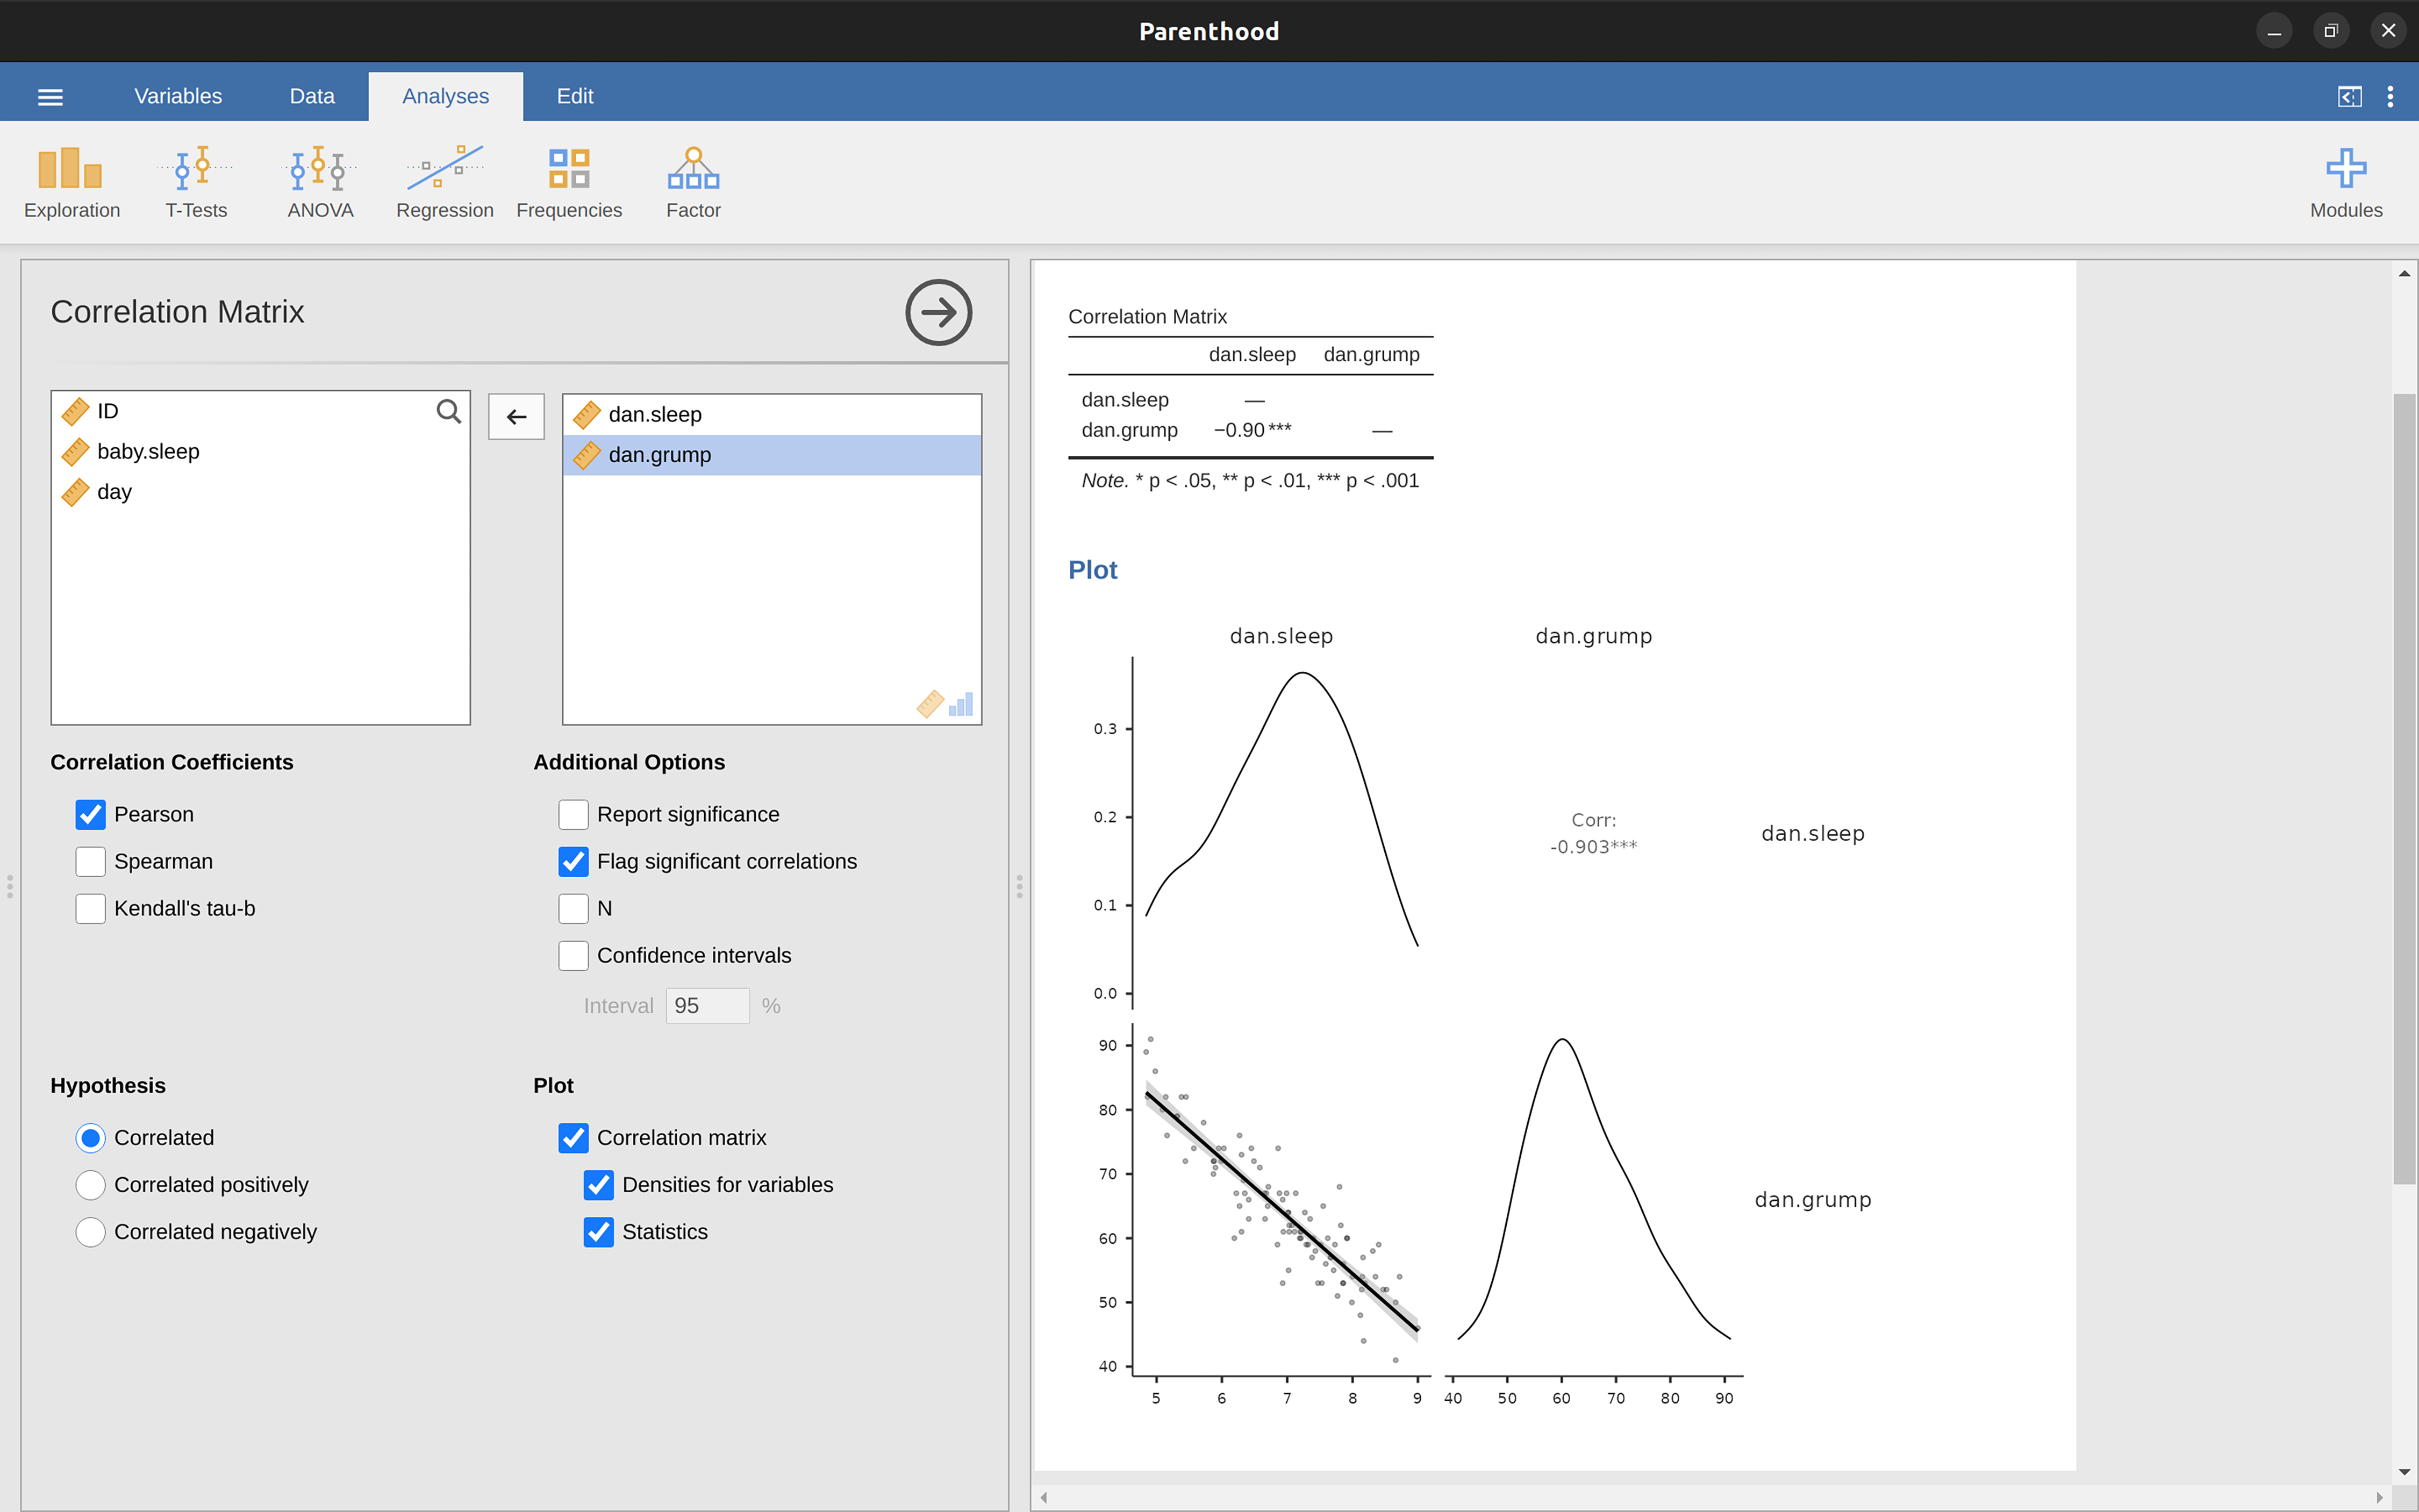
\includegraphics[width=1\textwidth,height=\textheight]{images/fig12-8.png} \hfill{}

\caption{\label{fig-fig12-8}Scatterplot via the `Correlation Matrix'
command in jamovi}

\end{figure}

The second way do to it is to use one of the jamovi add-on modules. This
module is called `scatr' and you can install it by clicking on the large
`\(+\)' icon in the top right of the jamovi screen, opening the jamovi
library, scrolling down until you find `scatr' and clicking `install'.
When you have done this, you will find a new `Scatterplot' command
available under the `Exploration' button. This plot is a bit different
than the first way, see Figure~\ref{fig-fig12-9}, but the important
information is the same.

\begin{figure}

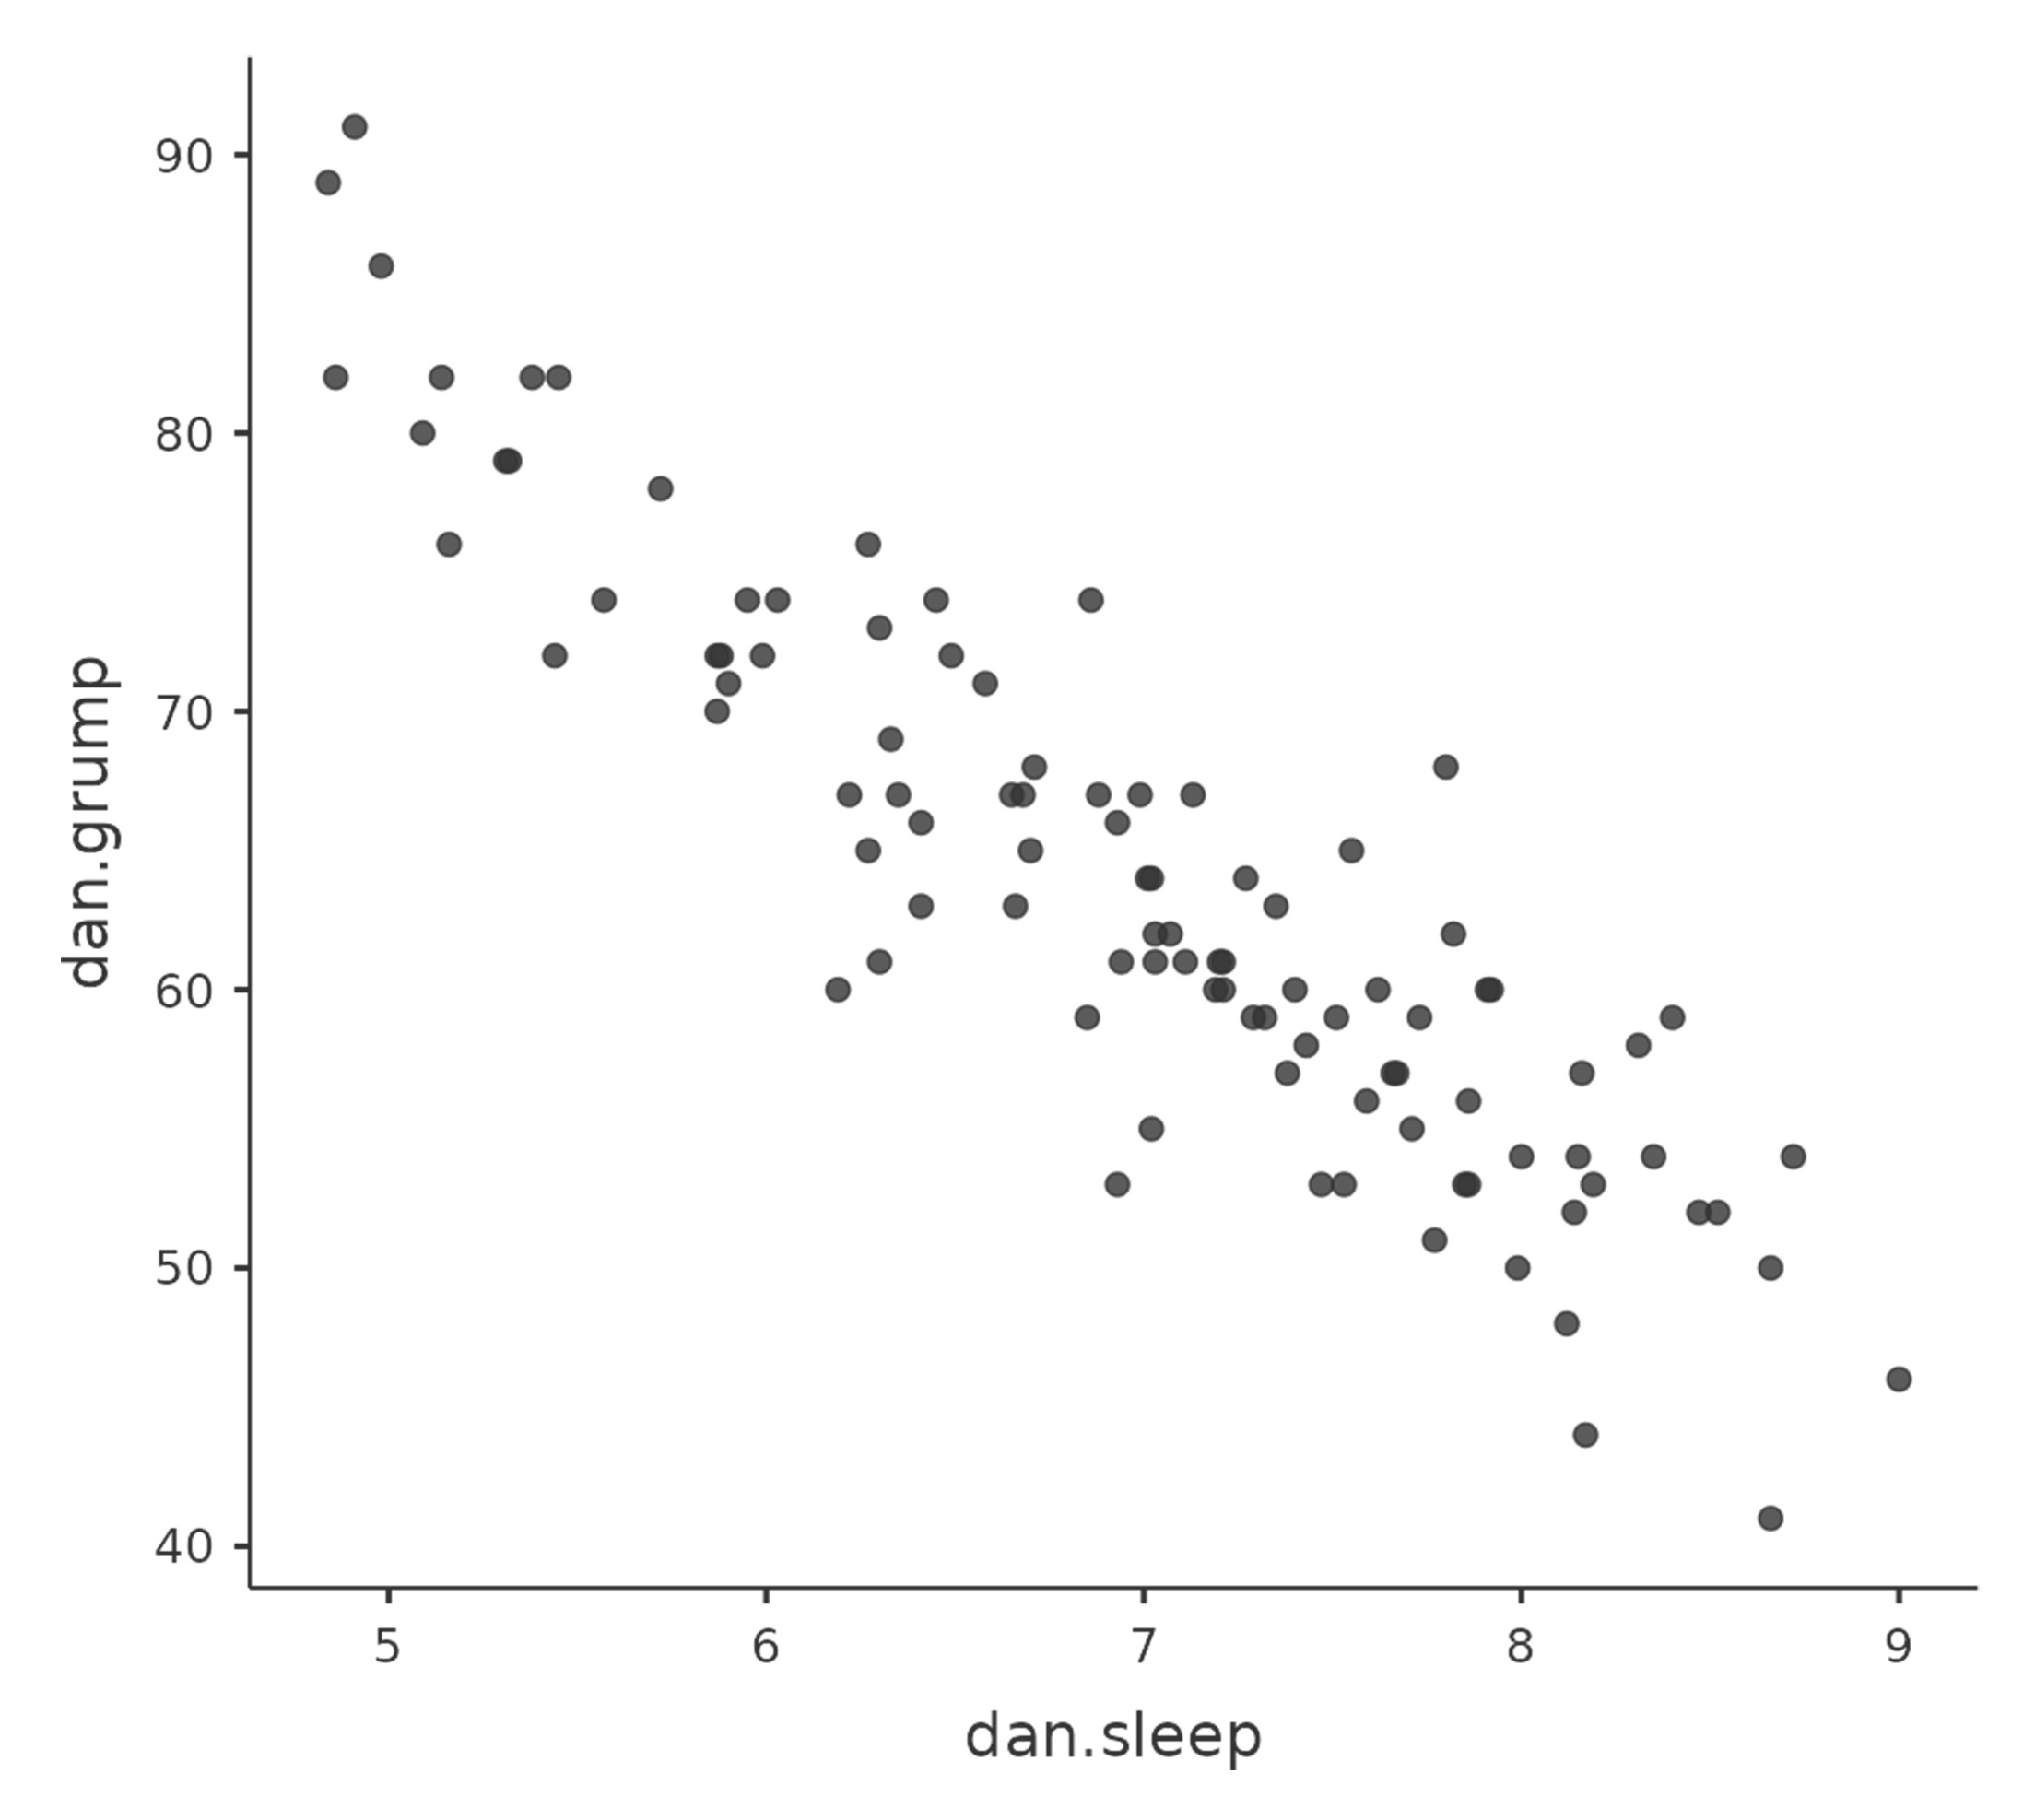
\includegraphics[width=1\textwidth,height=\textheight]{images/fig12-9.png} \hfill{}

\caption{\label{fig-fig12-9}Scatterplot via the `scatr' add-on module in
jamovi}

\end{figure}

\hypertarget{more-elaborate-options}{%
\subsection{More elaborate options}\label{more-elaborate-options}}

Often you will want to look at the relationships between several
variables at once, using a \textbf{scatterplot matrix} (in jamovi via
the `Correlation Matrix' - `Plot' command). Just add another variable,
for example baby.sleep to the list of variables to be correlated, and
jamovi will create a scatterplot matrix for you, just like the one in
Figure~\ref{fig-fig12-10}.

\begin{figure}

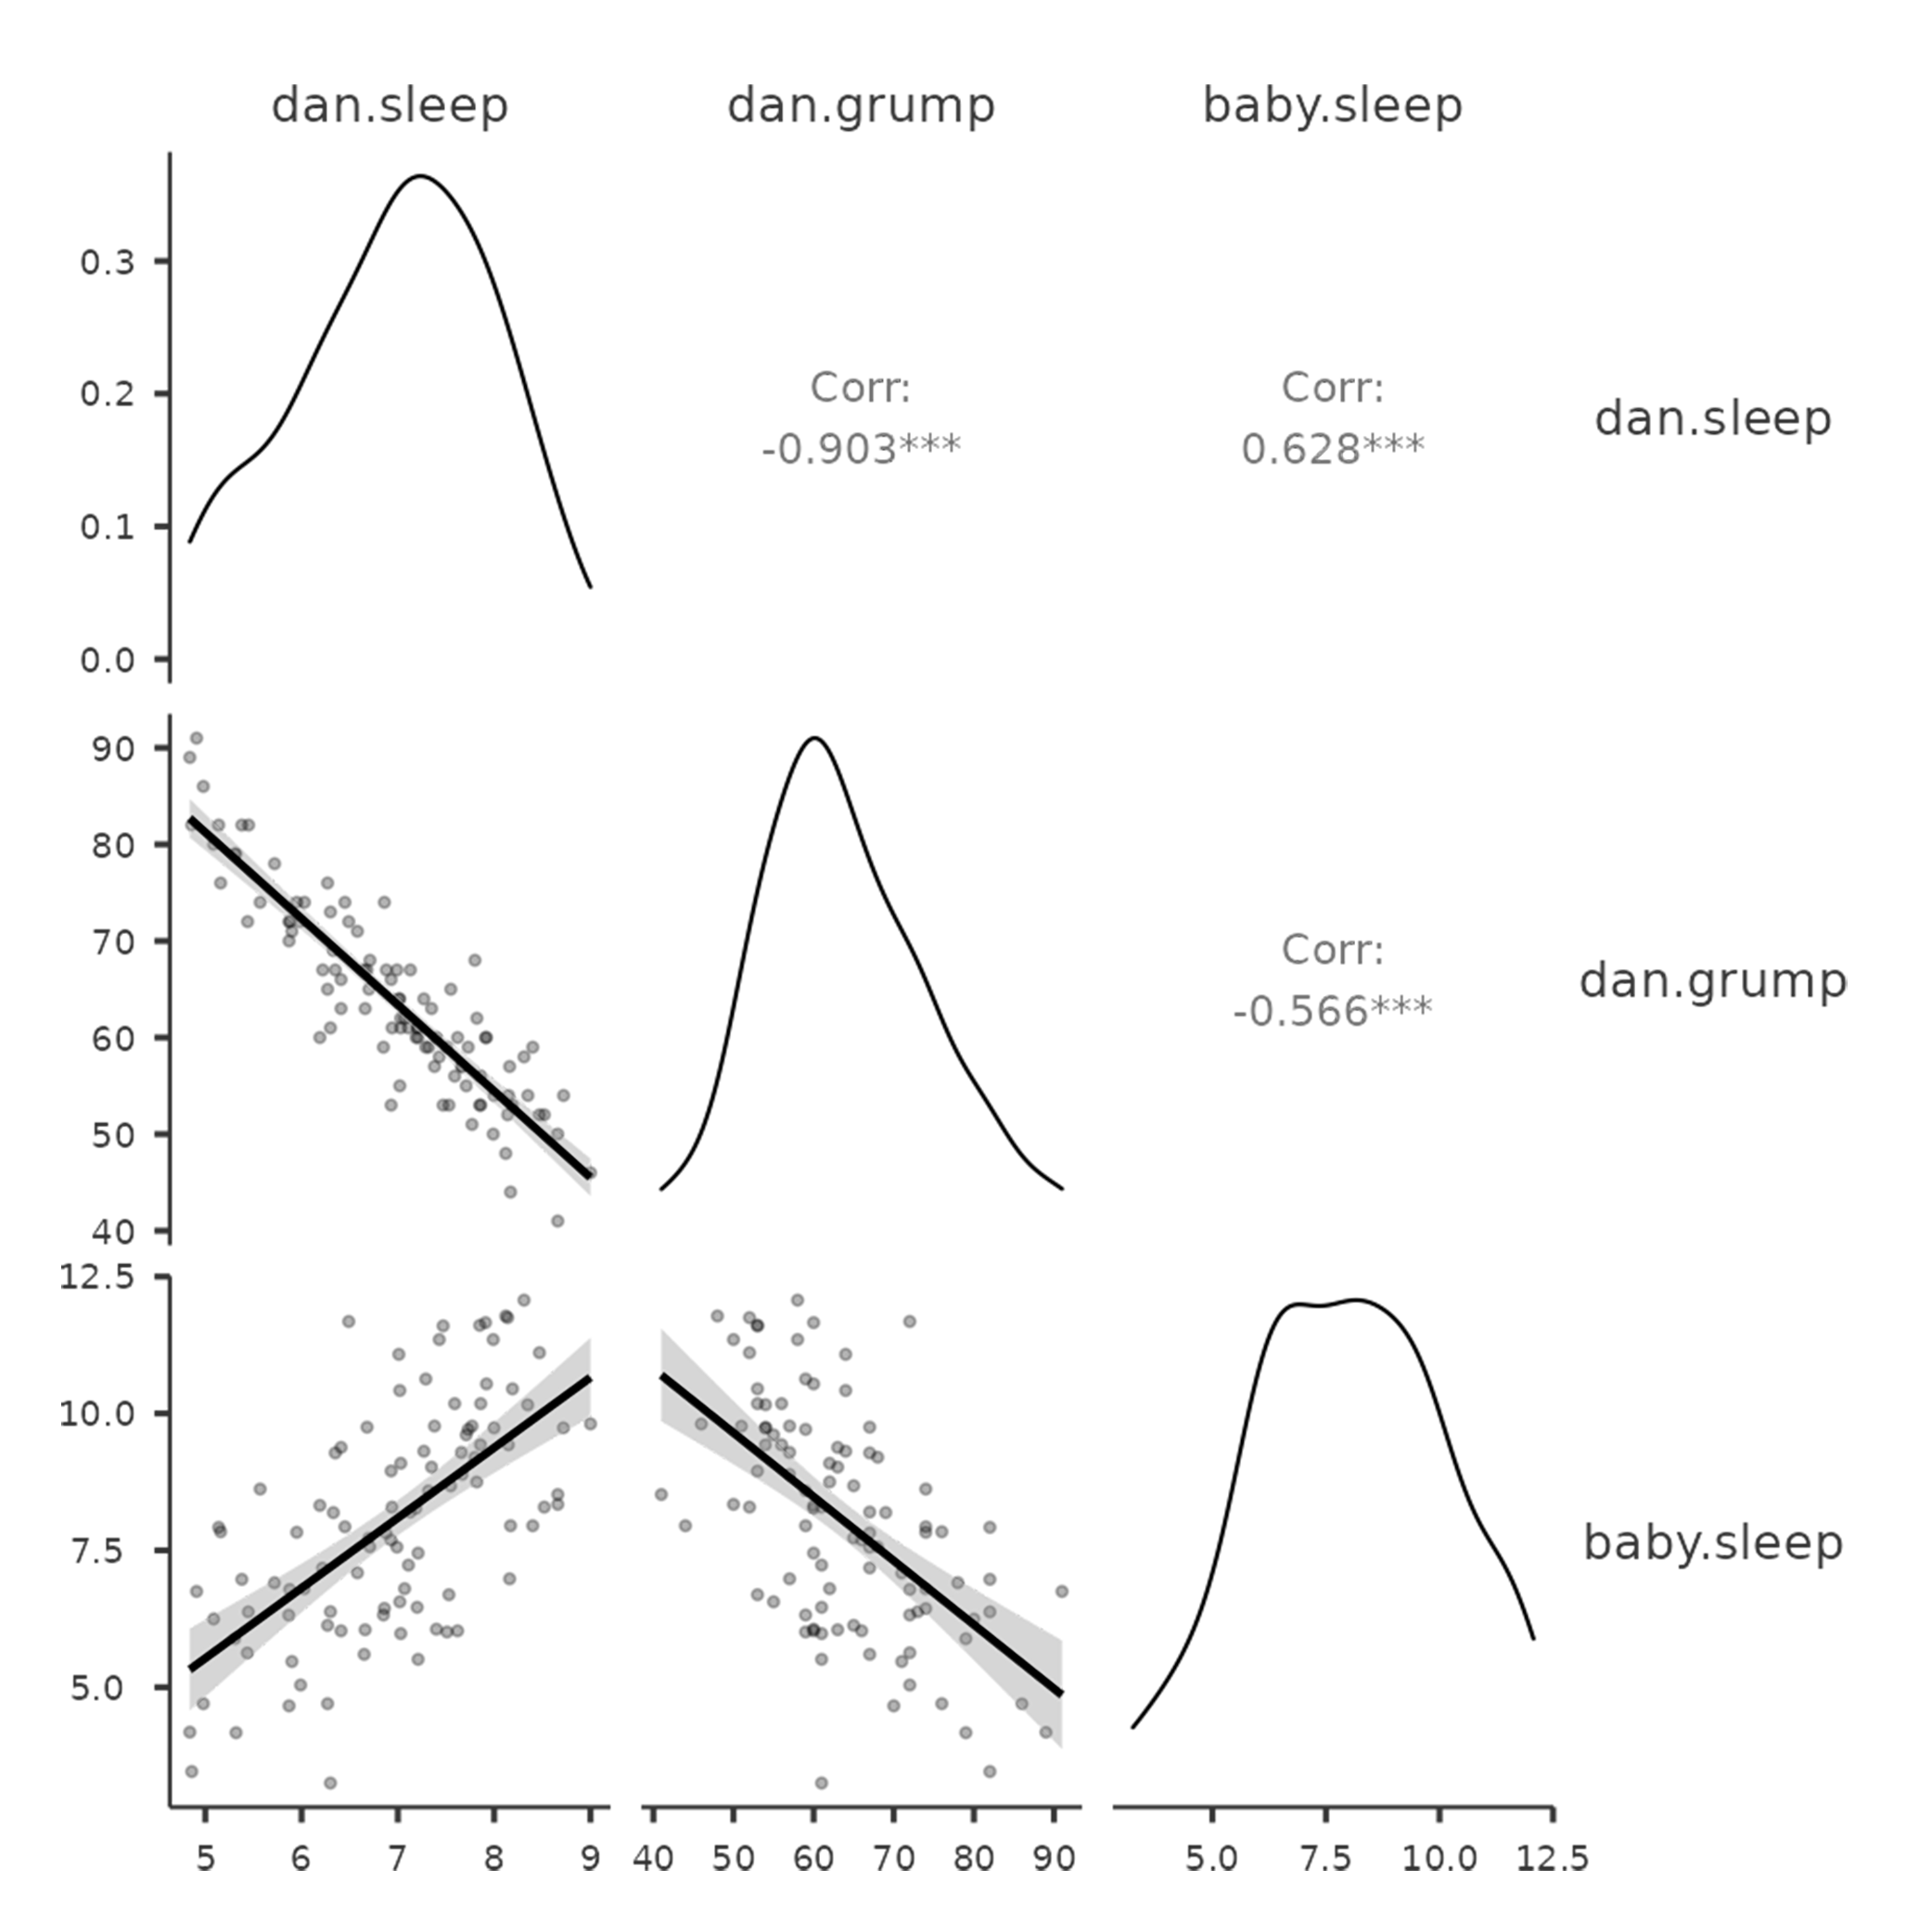
\includegraphics[width=1\textwidth,height=\textheight]{images/fig12-10.png} \hfill{}

\caption{\label{fig-fig12-10}A matrix of scatterplots produced using
jamovi}

\end{figure}

\hypertarget{what-is-a-linear-regression-model}{%
\section{What is a linear regression
model?}\label{what-is-a-linear-regression-model}}

Stripped to its bare essentials, linear regression models are basically
a slightly fancier version of the Pearson correlation (see
\protect\hyperlink{correlations}{Correlations}), though as we'll see
regression models are much more powerful tools.

Since the basic ideas in regression are closely tied to correlation,
we'll return to the \emph{parenthood.csv} file that we were using to
illustrate how correlations work. Recall that, in this data set we were
trying to find out why Dani is so very grumpy all the time and our
working hypothesis was that I'm not getting enough sleep. We drew some
scatterplots to help us examine the relationship between the amount of
sleep I get and my grumpiness the following day, as in
Figure~\ref{fig-fig12-9}, and as we saw previously this corresponds to a
correlation of \(r = -.90\), but what we find ourselves secretly
imagining is something that looks closer to Figure~\ref{fig-fig12-11}
(a). That is, we mentally draw a straight line through the middle of the
data. In statistics, this line that we're drawing is called a
\textbf{regression line}. Notice that, since we're not idiots, the
regression line goes through the middle of the data. We don't find
ourselves imagining anything like the rather silly plot shown in
Figure~\ref{fig-fig12-11} (b).

\begin{figure}

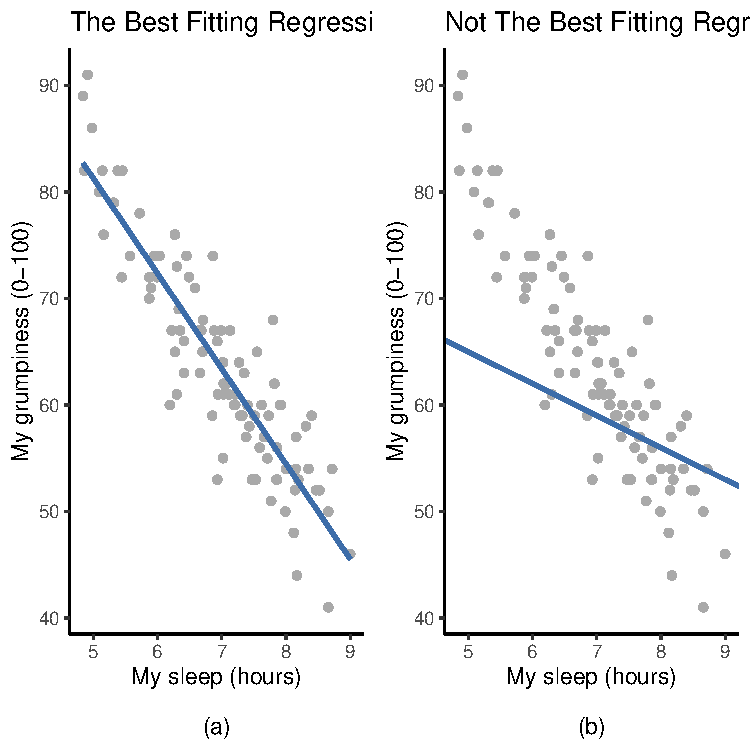
\includegraphics[width=1\textwidth,height=\textheight]{12-Correlation-and-linear-regression_files/figure-pdf/fig-fig12-11-1.pdf} \hfill{}

\caption{\label{fig-fig12-11}Panel (a) shows the sleep-grumpiness
scatterplot from Figure~\ref{fig-fig12-9} with the best fitting
regression line drawn over the top. Not surprisingly, the line goes
through the middle of the data. In contrast, panel (b) shows the same
data, but with a very poor choice of regression line drawn over the top}

\end{figure}

This is not highly surprising. The line that I've drawn in
Figure~\ref{fig-fig12-11} (b) doesn't ``fit'' the data very well, so it
doesn't make a lot of sense to propose it as a way of summarising the
data, right? This is a very simple observation to make, but it turns out
to be very powerful when we start trying to wrap just a little bit of
maths around it. To do so, let's start with a refresher of some high
school maths. The formula for a straight line is usually written like
this

\[y=a+bx\]

The two variables are \(x\) and \(y\), and we have two coefficients,
\(a\) and \(b\).\footnote{Also sometimes written as \(y = mx + c\) where
  \(m\) is the slope coefficient and \(c\) is the intercept (constant)
  coefficient.} The coefficient \(a\) represents the y-intercept of the
line, and coefficient \(b\) represents the slope of the line. The
intercept is interpreted as ``the value of y that you get when
\(x = 0\)''. Similarly, a slope of b means that if you increase the
x-value by 1 unit, then the y-value goes up by b units, and a negative
slope means that the y-value would go down rather than up. We use the
exact same formula for a regression line. If \(Y\) is the outcome
variable (the DV) and \(X\) is the predictor variable (the \(IV\)), then
the formula that describes our regression is written like this

\[\hat{Y}_i=b_0+b_1X_i\]

Hmm. Looks like the same formula, but there's some extra frilly bits in
this version. Let's make sure we understand them. Firstly, notice that
I've written \(X_i\) and \(Y_i\) rather than just plain old \(X\) and
\(Y\) . This is because we want to remember that we're dealing with
actual data. In this equation, \(X_i\) is the value of predictor
variable for the ith observation (i.e., the number of hours of sleep
that I got on day i of my little study), and \(Y_i\) is the
corresponding value of the outcome variable (i.e., my grumpiness on that
day). And although I haven't said so explicitly in the equation, what
we're assuming is that this formula works for all observations in the
data set (i.e., for all i). Secondly, notice that I wrote \(\hat{Y}_i\)
and not \(Y_i\) . This is because we want to make the distinction
between the actual data \(Y_i\), and the estimate \(\hat{Y}_i\) (i.e.,
the prediction that our regression line is making). Thirdly, I changed
the letters used to describe the coefficients from a and \(b\) to
\(b_0\) and \(b_1\). That's just the way that statisticians like to
refer to the coefficients in a regression model. I've no idea why they
chose b, but that's what they did. In any case \(b_0\) always refers to
the intercept term, and \(b_1\) refers to the slope.

Excellent, excellent. Next, I can't help but notice that, regardless of
whether we're talking about the good regression line or the bad one, the
data don't fall perfectly on the line. Or, to say it another way, the
data \(Y_i\) are not identical to the predictions of the regression
model \(\hat{Y}_i\). Since statisticians love to attach letters, names
and numbers to everything, let's refer to the difference between the
model prediction and that actual data point as a residual, and we'll
refer to it as \(\epsilon_i\).\footnote{The \(\epsilon\) symbol is the
  Greek letter epsilon. It's traditional to use \(\epsilon_i\) or
  \(e_i\) to denote a residual.} Written using mathematics, the
residuals are defined as

\[\epsilon_i=Y_i-\hat{Y}_i\]

which in turn means that we can write down the complete linear
regression model as

\[Y_i=b_0+b_1X_i+\epsilon_i\]

\hypertarget{estimating-a-linear-regression-model}{%
\section{Estimating a linear regression
model}\label{estimating-a-linear-regression-model}}

Okay, now let's redraw our pictures but this time I'll add some lines to
show the size of the residual for all observations. When the regression
line is good, our residuals (the lengths of the solid black lines) all
look pretty small, as shown in Figure~\ref{fig-fig12-12} (a), but when
the regression line is a bad one the residuals are a lot larger, as you
can see from looking at Figure~\ref{fig-fig12-12} (b). Hmm. Maybe what
we ``want'' in a regression model is \emph{small} residuals. Yes, that
does seem to make sense. In fact, I think I'll go so far as to say that
the ``best fitting'' regression line is the one that has the smallest
residuals. Or, better yet, since statisticians seem to like to take
squares of everything why not say that:

\begin{quote}
The estimated regression coefficients, \(\hat{b}_0\) and \(\hat{b}_1\),
are those that minimise the sum of the squared residuals, which we could
either write as \(\sum_i (Y_i - \hat{Y}_i)^2\) or as
\(\sum_i \epsilon_i^2\).
\end{quote}

\begin{figure}

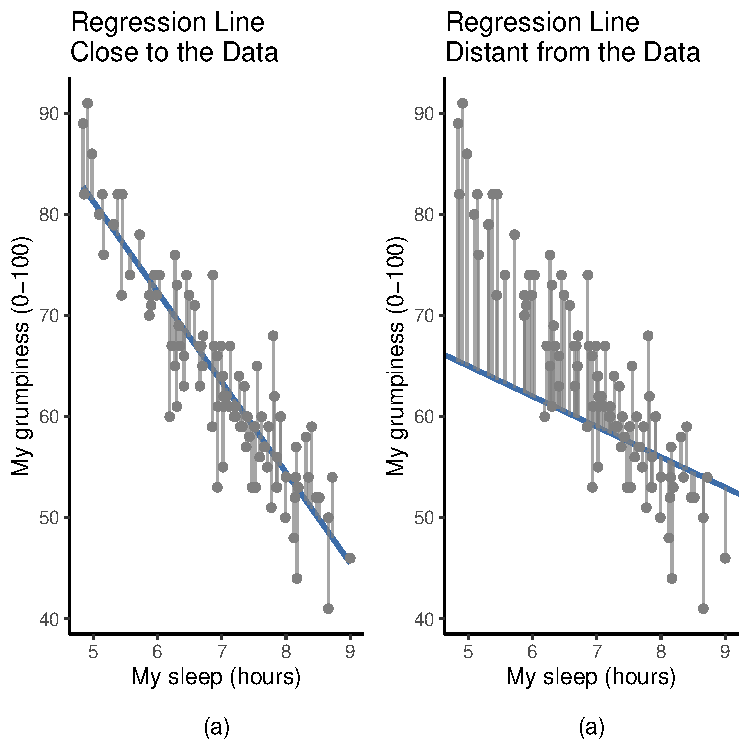
\includegraphics[width=1\textwidth,height=\textheight]{12-Correlation-and-linear-regression_files/figure-pdf/fig-fig12-12-1.pdf} \hfill{}

\caption{\label{fig-fig12-12}A depiction of the residuals associated
with the best fitting regression line (panel a), and the residuals
associated with a poor regression line (panel b). The residuals are much
smaller for the good regression line. Again, this is no surprise given
that the good line is the one that goes right through the middle of the
data}

\end{figure}

Yes, yes that sounds even better. And since I've indented it like that,
it probably means that this is the right answer. And since this is the
right answer, it's probably worth making a note of the fact that our
regression coefficients are estimates (we're trying to guess the
parameters that describe a population!), which is why I've added the
little hats, so that we get \(\hat{b}_0\) and \(\hat{b}_1\) rather than
\(b_0\) and \(b_1\). Finally, I should also note that, since there's
actually more than one way to estimate a regression model, the more
technical name for this estimation process is \textbf{ordinary least
squares (OLS) regression}.

At this point, we now have a concrete definition for what counts as our
``best'' choice of regression coefficients, \(\hat{b}_0\) and
\(\hat{b}_1\). The natural question to ask next is, if our optimal
regression coefficients are those that minimise the sum squared
residuals, how do we find these wonderful numbers? The actual answer to
this question is complicated and doesn't help you understand the logic
of regression.\footnote{Or at least, I'm assuming that it doesn't help
  most people. But on the off chance that someone reading this is a
  proper kung fu master of linear algebra (and to be fair, I always have
  a few of these people in my intro stats class), it will help you to
  know that the solution to the estimation problem turns out to be
  \(\hat{b} = (X^{'}X)^{-1}X^{'}y\), where \(\hat{b}\) is a vector
  containing the estimated regression coefficients, \(X\) is the
  ``design matrix'' that contains the predictor variables (plus an
  additional column containing all ones; strictly \(X\) is a matrix of
  the regressors, but I haven't discussed the distinction yet), and
  \(y\) is a vector containing the outcome variable. For everyone else,
  this isn't exactly helpful and can be downright scary. However, since
  quite a few things in linear regression can be written in linear
  algebra terms, you'll see a bunch of footnotes like this one in this
  chapter. If you can follow the maths in them, great. If not, ignore
  it.} This time I'm going to let you off the hook. Instead of showing
you the long and tedious way first and then ``revealing'' the wonderful
shortcut that jamovi provides, let's cut straight to the chase and just
use jamovi to do all the heavy lifting.

\hypertarget{linear-regression-in-jamovi}{%
\subsection{Linear regression in
jamovi}\label{linear-regression-in-jamovi}}

To run my linear regression, open up the `Regression' - `Linear
Regression' analysis in jamovi, using the \emph{parenthood.csv} data
file. Then specify dani.grump as the `Dependent Variable' and dani.sleep
as the variable entered in the `Covariates' box. This gives the results
shown in Figure~\ref{fig-fig12-13}, showing an intercept
\(\hat{b}_0 = 125.96\) and the slope \(\hat{b}_1 = -8.94\). In other
words, the best fitting regression line that I plotted in
Figure~\ref{fig-fig12-11} has this formula:

\[\hat{Y}_i=125.96+(-8.94 X_i)\]

\begin{figure}

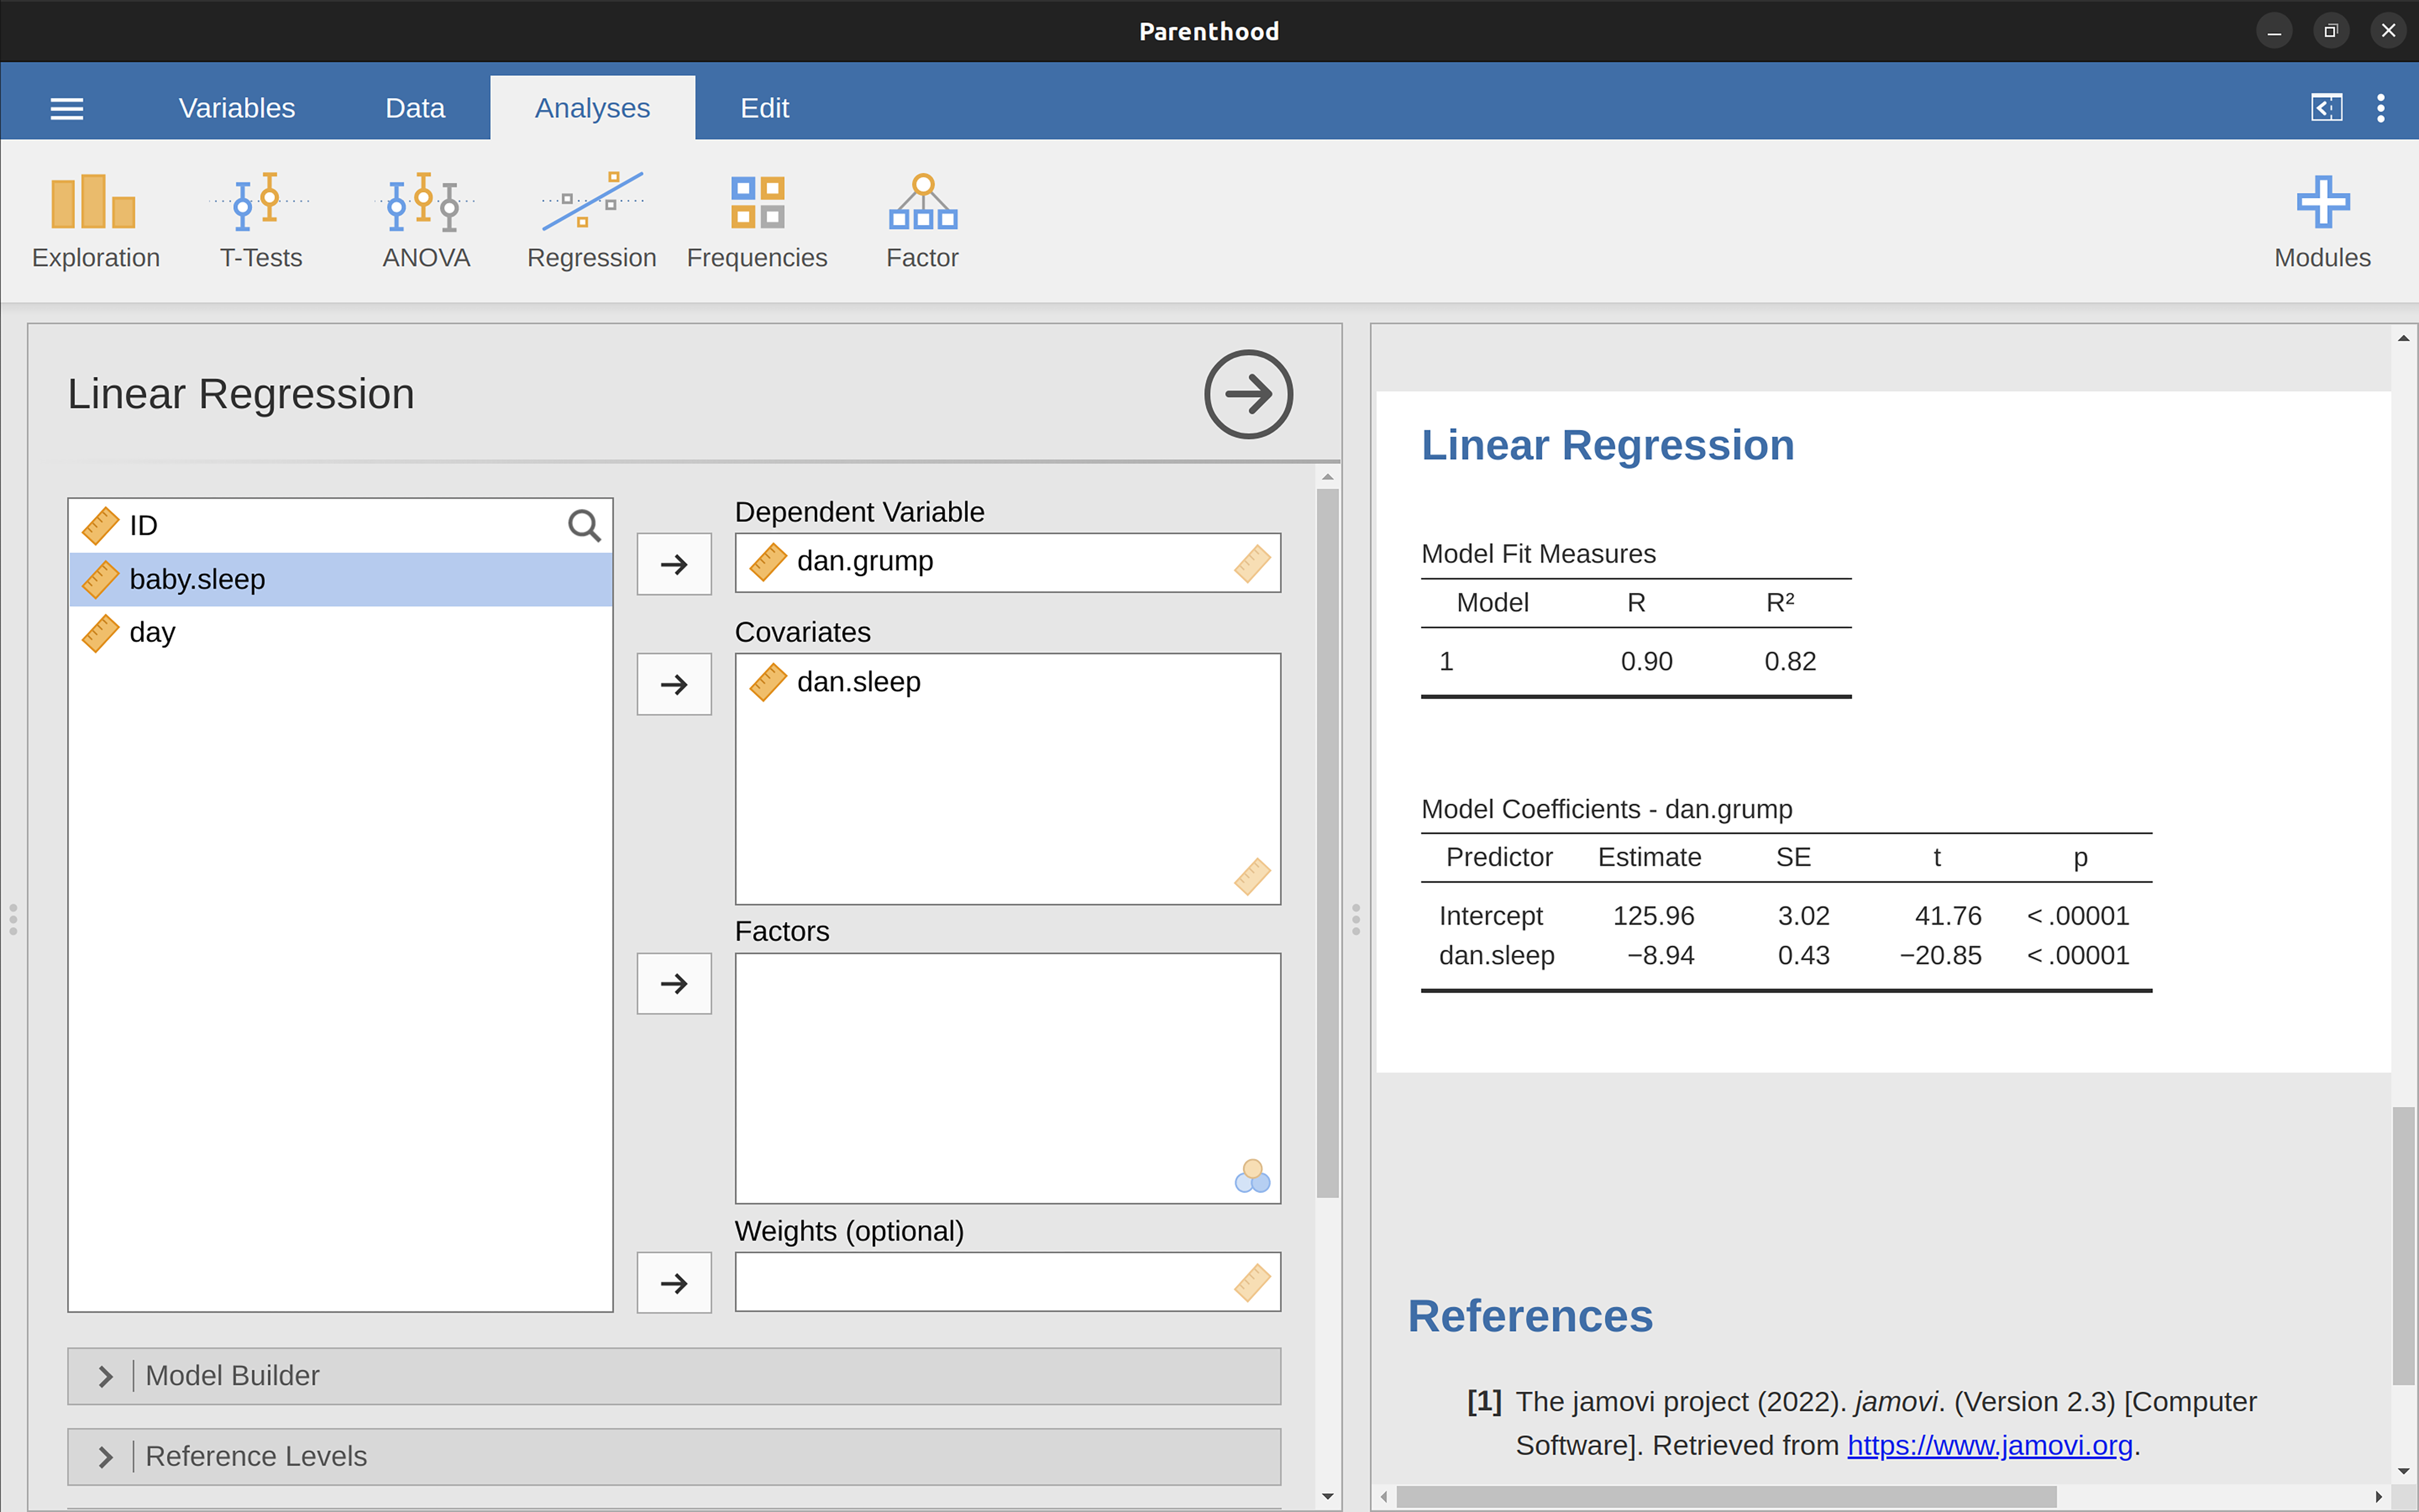
\includegraphics[width=1\textwidth,height=\textheight]{images/fig12-13.png} \hfill{}

\caption{\label{fig-fig12-13}A jamovi screenshot showing a simple linear
regression analysis}

\end{figure}

\hypertarget{interpreting-the-estimated-model}{%
\subsection{Interpreting the estimated
model}\label{interpreting-the-estimated-model}}

The most important thing to be able to understand is how to interpret
these coefficients. Let's start with \(\hat{b}_1\), the slope. If we
remember the definition of the slope, a regression coefficient of
\(\hat{b}_1 = -8.94\) means that if I increase \(X_i\) by 1, then I'm
decreasing \(Y_i\) by 8.94. That is, each additional hour of sleep that
I gain will improve my mood, reducing my grumpiness by 8.94 grumpiness
points. What about the intercept? Well, since \(\hat{b}_0\) corresponds
to ``the expected value of \(Y_i\) when \(X_i\) equals 0'', it's pretty
straightforward. It implies that if I get zero hours of sleep
(\(X_i = 0\)) then my grumpiness will go off the scale, to an insane
value of (\(Y_i = 125.96\)). Best to be avoided, I think.

\hypertarget{multiple-linear-regression}{%
\section{Multiple linear regression}\label{multiple-linear-regression}}

The simple linear regression model that we've discussed up to this point
assumes that there's a single predictor variable that you're interested
in, in this case dani.sleep. In fact, up to this point every statistical
tool that we've talked about has assumed that your analysis uses one
predictor variable and one outcome variable. However, in many (perhaps
most) research projects you actually have multiple predictors that you
want to examine. If so, it would be nice to be able to extend the linear
regression framework to be able to include multiple predictors. Perhaps
some kind of \textbf{multiple regression} model would be in order?

Multiple regression is conceptually very simple. All we do is add more
terms to our regression equation. Let's suppose that we've got two
variables that we're interested in; perhaps we want to use both
dani.sleep and baby.sleep to predict the dani.grump variable. As before,
we let \(Y_{i}\) refer to my grumpiness on the i-th day. But now we have
two \$ X \$ variables: the first corresponding to the amount of sleep I
got and the second corresponding to the amount of sleep my son got. So
we'll let \(X_{i1}\) refer to the hours I slept on the i-th day and
\(X_{i2}\) refers to the hours that the baby slept on that day. If so,
then we can write our regression model like this:

\[Y_i=b_0+b_1X_{i1}+b_2X_{i2}+\epsilon_i\]

As before, \(\epsilon_i\) is the residual associated with the i-th
observation, \(\epsilon_i = Y_i - \hat{Y}_i\). In this model, we now
have three coefficients that need to be estimated: \(b_0\) is the
intercept, \(b_1\) is the coefficient associated with my sleep, and
\(b_2\) is the coefficient associated with my son's sleep. However,
although the number of coefficients that need to be estimated has
changed, the basic idea of how the estimation works is unchanged: our
estimated coefficients \(\hat{b}_0\), \(\hat{b}_1\) and \(\hat{b}_2\)
are those that minimise the sum squared residuals.

\hypertarget{doing-it-in-jamovi}{%
\subsection{Doing it in jamovi}\label{doing-it-in-jamovi}}

Multiple regression in jamovi is no different to simple regression. All
we have to do is add additional variables to the `Covariates' box in
jamovi. For example, if we want to use both dani.sleep and baby.sleep as
predictors in our attempt to explain why I'm so grumpy, then move
baby.sleep across into the `Covariates' box alongside dani.sleep. By
default, jamovi assumes that the model should include an intercept. The
coefficients we get this time are shown in Table~\ref{tbl-tab12-4}.

\hypertarget{tbl-tab12-4}{}
 
  \providecommand{\huxb}[2]{\arrayrulecolor[RGB]{#1}\global\arrayrulewidth=#2pt}
  \providecommand{\huxvb}[2]{\color[RGB]{#1}\vrule width #2pt}
  \providecommand{\huxtpad}[1]{\rule{0pt}{#1}}
  \providecommand{\huxbpad}[1]{\rule[-#1]{0pt}{#1}}

\begin{table}[ht]
\caption{\label{tbl-tab12-4}Adding multiple variables as predictors in a regression }\tabularnewline

\begin{centerbox}
\begin{threeparttable}
\setlength{\tabcolsep}{0pt}
\begin{tabularx}{0.9\textwidth}{p{0.3\textwidth} p{0.3\textwidth} p{0.3\textwidth}}


\hhline{>{\huxb{0, 0, 0}{0.4}}->{\huxb{0, 0, 0}{0.4}}->{\huxb{0, 0, 0}{0.4}}-}
\arrayrulecolor{black}

\multicolumn{1}{!{\huxvb{0, 0, 0}{0}}p{0.3\textwidth}!{\huxvb{0, 0, 0}{0}}}{\hspace{0pt}\parbox[b]{0.3\textwidth-0pt-12pt}{\huxtpad{2pt + 1em}\centering \textbf{(Intercept)}\huxbpad{2pt}}} &
\multicolumn{1}{p{0.3\textwidth}!{\huxvb{0, 0, 0}{0}}}{\hspace{12pt}\parbox[b]{0.3\textwidth-12pt-12pt}{\huxtpad{2pt + 1em}\centering \textbf{dani.sleep}\huxbpad{2pt}}} &
\multicolumn{1}{p{0.3\textwidth}!{\huxvb{0, 0, 0}{0}}}{\hspace{12pt}\parbox[b]{0.3\textwidth-12pt-0pt}{\huxtpad{2pt + 1em}\centering \textbf{baby.sleep}\huxbpad{2pt}}} \tabularnewline[-0.5pt]


\hhline{>{\huxb{0, 0, 0}{0.4}}->{\huxb{0, 0, 0}{0.4}}->{\huxb{0, 0, 0}{0.4}}-}
\arrayrulecolor{black}

\multicolumn{1}{!{\huxvb{0, 0, 0}{0}}p{0.3\textwidth}!{\huxvb{0, 0, 0}{0}}}{\hspace{0pt}\parbox[b]{0.3\textwidth-0pt-12pt}{\huxtpad{2pt + 1em}\centering 125.97\huxbpad{2pt}}} &
\multicolumn{1}{p{0.3\textwidth}!{\huxvb{0, 0, 0}{0}}}{\hspace{12pt}\parbox[b]{0.3\textwidth-12pt-12pt}{\huxtpad{2pt + 1em}\centering -8.95\huxbpad{2pt}}} &
\multicolumn{1}{p{0.3\textwidth}!{\huxvb{0, 0, 0}{0}}}{\hspace{12pt}\parbox[b]{0.3\textwidth-12pt-0pt}{\huxtpad{2pt + 1em}\centering 0.01\huxbpad{2pt}}} \tabularnewline[-0.5pt]


\hhline{>{\huxb{0, 0, 0}{0.4}}->{\huxb{0, 0, 0}{0.4}}->{\huxb{0, 0, 0}{0.4}}-}
\arrayrulecolor{black}
\end{tabularx} 

\end{threeparttable}\par\end{centerbox}

\end{table}
 

The coefficient associated with dani.sleep is quite large, suggesting
that every hour of sleep I lose makes me a lot grumpier. However, the
coefficient for baby.sleep is very small, suggesting that it doesn't
really matter how much sleep my son gets. What matters as far as my
grumpiness goes is how much sleep I get. To get a sense of what this
multiple regression model looks like, Figure~\ref{fig-fig12-14} shows a
3D plot that plots all three variables, along with the regression model
itself.

\begin{figure}

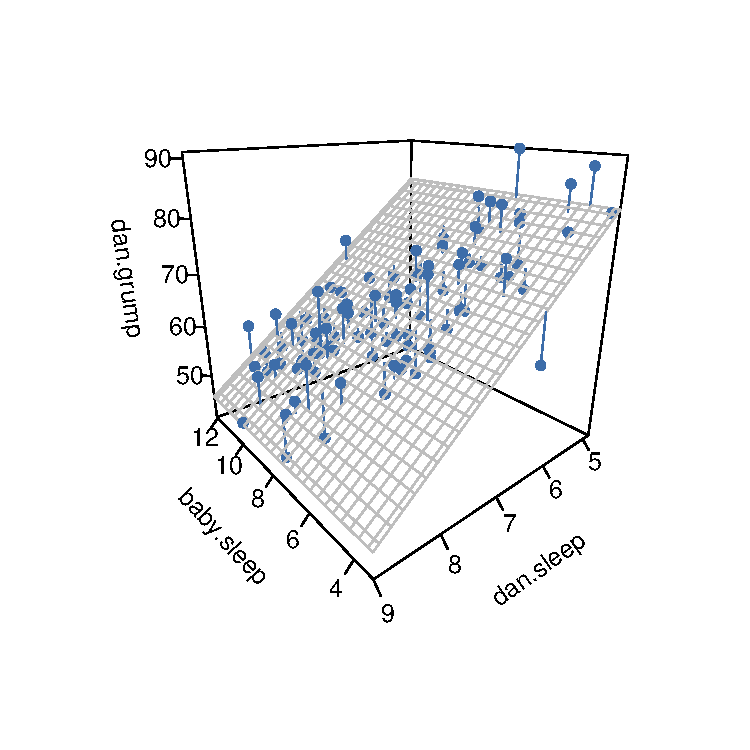
\includegraphics[width=1\textwidth,height=\textheight]{12-Correlation-and-linear-regression_files/figure-pdf/fig-fig12-14-1.pdf} \hfill{}

\caption{\label{fig-fig12-14}A 3D visualisation of a multiple regression
model. There are two predictors in the model, dani.sleep and baby.sleep
and the outcome variable is dani.grump. Together, these three variables
form a 3D space. Each observation (dot) is a point in this space. In
much the same way that a simple linear regression model forms a line in
2D space, this multiple regression model forms a plane in 3D space. When
we estimate the regression coefficients what we're trying to do is find
a plane that is as close to all the blue dots as possible}

\end{figure}

{[}Additional technical detail\footnote{The formula for the general
  case: The equation that I gave in the main text shows you what a
  multiple regression model looks like when you include two predictors.
  Not surprisingly then, if you want more than two predictors all you
  have to do is add more \(X\) terms and more \(b\) coefficients. In
  other words, if you have \(K\) predictor variables in the model then
  the regression equation look like this
  \[Y_i=b_0+(\sum_{k=1}^{K}b_k X_{ik})+\epsilon_i\]}{]}

\hypertarget{quantifying-the-fit-of-the-regression-model}{%
\section{Quantifying the fit of the regression
model}\label{quantifying-the-fit-of-the-regression-model}}

So we now know how to estimate the coefficients of a linear regression
model. The problem is, we don't yet know if this regression model is any
good. For example, the regression.1 model claims that every hour of
sleep will improve my mood by quite a lot, but it might just be rubbish.
Remember, the regression model only produces a prediction \(\hat{Y}_i\)
about what my mood is like, but my actual mood is \(Y_i\) . If these two
are very close, then the regression model has done a good job. If they
are very different, then it has done a bad job.

\hypertarget{sec-The-R2-value}{%
\subsection{\texorpdfstring{The \(R^2\)
value}{The R\^{}2 value}}\label{sec-The-R2-value}}

Once again, let's wrap a little bit of mathematics around this. Firstly,
we've got the sum of the squared residuals

\[SS_{res}=\sum_i (Y_i-\hat{Y_i})^2\]

which we would hope to be pretty small. Specifically, what we'd like is
for it to be very small in comparison to the total variability in the
outcome variable

\[SS_{tot}=\sum_i(Y_i-\bar{Y})^2\]

While we're here, let's calculate these values ourselves, not by hand
though. Let's use something like Excel or another standard spreadsheet
programme. I have done this by opening up the \emph{parenthood.csv} file
in Excel and saving it as parenthood rsquared.xls so that I can work on
it. The first thing to do is calculate the \(\hat{Y}\) values, and for
the simple model that uses only a single predictor we would do the
following:

\begin{enumerate}
\def\labelenumi{\arabic{enumi}.}
\tightlist
\item
  create a new column called `Y.pred' using the formula `= 125.97 +
  (-8.94 \(\times\) dani.sleep)'.
\item
  calculate the SS(resid) by creating a new column called
  `(Y-Y.pred)\^{}2' using the formula ' = (dani.grump - Y.pred)\^{}2 '.
\item
  Then, at the bottom of this column calculate the sum of these values,
  i.e.~' sum( ( Y-Y.pred)\^{}2 ).
\item
  At the bottom of the dani.grump column, calculate the mean value for
  dani.grump (NB Excel uses the word ' AVERAGE ' rather than `mean' in
  its function).
\item
  Then create a new column, called ' (Y - mean(Y))\^{}2 )' using the
  formula ' = (dani.grump - AVERAGE(dani.grump))\^{}2 '.
\item
  Then, at the bottom of this column calculate the sum of these values,
  i.e.~`sum( (Y - mean(Y))\^{}2 )'.
\item
  Calculate R.squared by typing into a blank cell the following: `= 1 -
  (SS(resid) / SS(tot) )'.
\end{enumerate}

This gives a value for \(R^2\) of `0.8161018'. The \(R^2\) value,
sometimes called the \textbf{coefficient of determination}\footnote{And
  by ``sometimes'' I mean ``almost never''. In practice everyone just
  calls it ``R-squared''.} has a simple interpretation: it is the
proportion of the variance in the outcome variable that can be accounted
for by the predictor. So, in this case the fact that we have obtained
\(R^2 = .816\) means that the predictor (my.sleep) explains \(81.6\%\)
of the variance in the outcome (my.grump).

Naturally, you don't actually need to type all these commands into Excel
yourself if you want to obtain the \(R^2\) value for your regression
model. As we'll see later on in the section on
\protect\hyperlink{running-the-hypothesis-tests-in-jamovi}{Running the
hypothesis tests in jamovi}, all you need to do is specify this as an
option in jamovi. However, let's put that to one side for the moment.
There's another property of \(R^2\) that I want to point out.

\hypertarget{the-relationship-between-regression-and-correlation}{%
\subsection{The relationship between regression and
correlation}\label{the-relationship-between-regression-and-correlation}}

At this point we can revisit my earlier claim that regression, in this
very simple form that I've discussed so far, is basically the same thing
as a correlation. Previously, we used the symbol \(r\) to denote a
Pearson correlation. Might there be some relationship between the value
of the correlation coefficient \(r\) and the \(R^2\) value from linear
regression? Of course there is: the squared correlation \(r^2\) is
identical to the \(R^2\) value for a linear regression with only a
single predictor. In other words, running a Pearson correlation is more
or less equivalent to running a linear regression model that uses only
one predictor variable.

\hypertarget{the-adjusted-r2-value}{%
\subsection{\texorpdfstring{The adjusted \(R^2\)
value}{The adjusted R\^{}2 value}}\label{the-adjusted-r2-value}}

One final thing to point out before moving on. It's quite common for
people to report a slightly different measure of model performance,
known as ``adjusted \(R^2\)''. The motivation behind calculating the
adjusted \(R^2\) value is the observation that adding more predictors
into the model will always cause the \(R^2\) value to increase (or at
least not decrease).

{[}Additional technical detail\footnote{The adjusted \(R^2\) value
  introduces a slight change to the calculation, as follows. For a
  regression model with \(K\) predictors, fit to a data set containing
  \(N\) observations, the adjusted \(R^2\) is:
  \[\text{adj.}R^2=1-(\frac{SS_{res}}{SS_{tot}} \times \frac{N-1}{N-K-1})\]}{]}

This adjustment is an attempt to take the degrees of freedom into
account. The big advantage of the adjusted \(R^2\) value is that when
you add more predictors to the model, the adjusted \(R^2\) value will
only increase if the new variables improve the model performance more
than you'd expect by chance. The big disadvantage is that the adjusted
\(R^2\) value can't be interpreted in the elegant way that \(R^2\) can.
\(R^2\) has a simple interpretation as the proportion of variance in the
outcome variable that is explained by the regression model. To my
knowledge, no equivalent interpretation exists for adjusted \(R^2\).

An obvious question then is whether you should report \(R^2\) or
adjusted \(R^2\). This is probably a matter of personal preference. If
you care more about interpretability, then \(R^2\) is better. If you
care more about correcting for bias, then adjusted \(R^2\) is probably
better. Speaking just for myself, I prefer \(R^2\). My feeling is that
it's more important to be able to interpret your measure of model
performance. Besides, as we'll see in
\protect\hyperlink{hypothesis-tests-for-regression-models}{Hypothesis
tests for regression models}, if you're worried that the improvement in
\(R^2\) that you get by adding a predictor is just due to chance and not
because it's a better model, well we've got hypothesis tests for that.

\hypertarget{hypothesis-tests-for-regression-models}{%
\section{Hypothesis tests for regression
models}\label{hypothesis-tests-for-regression-models}}

So far we've talked about what a regression model is, how the
coefficients of a regression model are estimated, and how we quantify
the performance of the model (the last of these, incidentally, is
basically our measure of effect size). The next thing we need to talk
about is hypothesis tests. There are two different (but related) kinds
of hypothesis tests that we need to talk about: those in which we test
whether the regression model as a whole is performing significantly
better than a null model, and those in which we test whether a
particular regression coefficient is significantly different from zero.

\hypertarget{testing-the-model-as-a-whole}{%
\subsection{Testing the model as a
whole}\label{testing-the-model-as-a-whole}}

Okay, suppose you've estimated your regression model. The first
hypothesis test you might try is the null hypothesis that there is no
relationship between the predictors and the outcome, and the alternative
hypothesis that the data are distributed in exactly the way that the
regression model predicts.

{[}Additional technical detail\footnote{Formally, our ``null model''
  corresponds to the fairly trivial ``regression'' model in which we
  include 0 predictors and only include the intercept term \(b_0\):
  \(H_0:Y_0=b_0+\epsilon_i\) If our regression model has \(K\)
  predictors, the ``alternative model'' is described using the usual
  formula for a multiple regression model:
  \[H_1:Y_i=b_0+(\sum_{k=1}^K b_k X_{ik})+\epsilon_i\] How can we test
  these two hypotheses against each other? The trick is to understand
  that it's possible to divide up the total variance \(SStot\) into the
  sum of the residual variance \(SSres\) and the regression model
  variance \(SSmod\). I'll skip over the technicalities, since we'll get
  to that later when we look at ANOVA in
  Chapter~\ref{sec-Comparing-several-means-one-way-ANOVA}. But just note
  that \(SS_{mod}=SS_{tot}-SS_{res}\) And we can convert the sums of
  squares into mean squares by dividing by the degrees of freedom.
  \[MS_{mod}=\frac{SS_{mod}}{df_{mod}}\]
  \[MS_{res}=\frac{SS_{res}}{df_{res}}\] So, how many degrees of freedom
  do we have? As you might expect the df associated with the model is
  closely tied to the number of predictors that we've included. In fact,
  it turns out that \(df_mod = K\). For the residuals the total degrees
  of freedom is \(df_res = N - K - 1\). Now that we've got our mean
  square values we can calculate an \(F\) statistic like this
  \[F=\frac{MS_{mod}}{MS_{res}}\] and the degrees of freedom associated
  with this are \(K\) and \(N - K - 1\).}{]}

We'll see much more of the \(F\) statistic in
Chapter~\ref{sec-Comparing-several-means-one-way-ANOVA}, but for now
just know that we can interpret large \(F\) values as indicating that
the null hypothesis is performing poorly in comparison to the
alternative hypothesis. In a moment I'll show you how to do the test in
jamovi the easy way, but first let's have a look at the tests for the
individual regression coefficients.

\hypertarget{tests-for-individual-coefficients}{%
\subsection{Tests for individual
coefficients}\label{tests-for-individual-coefficients}}

The \emph{F}-test that we've just introduced is useful for checking that
the model as a whole is performing better than chance. If your
regression model doesn't produce a significant result for the
\emph{F}-test then you probably don't have a very good regression model
(or, quite possibly, you don't have very good data). However, while
failing this test is a pretty strong indicator that the model has
problems, passing the test (i.e., rejecting the null) doesn't imply that
the model is good! Why is that, you might be wondering? The answer to
that can be found by looking at the coefficients for the
\protect\hyperlink{multiple-linear-regression}{Multiple linear
regression} model we have already looked at (Table~\ref{tbl-tab12-4})

I can't help but notice that the estimated regression coefficient for
the baby.sleep variable is tiny (\(0.01\)), relative to the value that
we get for dani.sleep (\(-8.95\)). Given that these two variables are
absolutely on the same scale (they're both measured in ``hours slept''),
I find this illuminating. In fact, I'm beginning to suspect that it's
really only the amount of sleep that I get that matters in order to
predict my grumpiness. We can re-use a hypothesis test that we discussed
earlier, the \(t\)-test. The test that we're interested in has a null
hypothesis that the true regression coefficient is zero (\(b = 0\)),
which is to be tested against the alternative hypothesis that it isn't
(\(b \neq 0\)). That is:

\[H_0:b=0\] \[H_1:b \neq 0\]

How can we test this? Well, if the central limit theorem is kind to us
we might be able to guess that the sampling distribution of \(\hat{b}\),
the estimated regression coefficient, is a normal distribution with mean
centred on \(b\). What that would mean is that if the null hypothesis
were true, then the sampling distribution of \(\hat{b}\) has mean zero
and unknown standard deviation. Assuming that we can come up with a good
estimate for the standard error of the regression coefficient,
\(se(\hat{b})\), then we're in luck. That's exactly the situation for
which we introduced the one-sample \(t\)-test back in
\textbf{?@sec-Comparing-two-means}. So let's define a \emph{t} statistic
like this

\[t=\frac{\hat{b}}{SE(\hat{b})}\]

I'll skip over the reasons why, but our degrees of freedom in this case
are \(df = N - K - 1\). Irritatingly, the estimate of the standard error
of the regression coefficient, \(se(\hat{b})\), is not as easy to
calculate as the standard error of the mean that we used for the simpler
\(t\)-tests in \textbf{?@sec-Comparing-two-means}. In fact, the formula
is somewhat ugly, and not terribly helpful to look at.\footnote{For
  advanced readers only. The vector of residuals is
  \(\epsilon=y - X\hat{b}\). For K predictors plus the intercept, the
  estimated residual variance is
  \(\hat{\sigma}^2 = \frac{\epsilon^{'}\epsilon}{(N - K - 1)}\). The
  estimated covariance matrix of the coefficients is
  \(\hat{\sigma}^{2}(X^{'}X)^{-1}\), the main diagonal of which is
  \(se(\hat{b})\), our estimated standard errors.} For our purposes it's
sufficient to point out that the standard error of the estimated
regression coefficient depends on both the predictor and outcome
variables, and it is somewhat sensitive to violations of the homogeneity
of variance assumption (discussed shortly).

In any case, this \emph{t} statistic can be interpreted in the same way
as the \emph{t} statistics that we discussed in
\textbf{?@sec-Comparing-two-means}. Assuming that you have a two-sided
alternative (i.e., you don't really care if b \(>\) 0 or b \(<\) 0),
then it's the extreme values of t (i.e., a lot less than zero or a lot
greater than zero) that suggest that you should reject the null
hypothesis.

\hypertarget{running-the-hypothesis-tests-in-jamovi}{%
\subsection{Running the hypothesis tests in
jamovi}\label{running-the-hypothesis-tests-in-jamovi}}

To compute all of the statistics that we have talked about so far, all
you need to do is make sure the relevant options are checked in jamovi
and then run the regression. If we do that, as in
Figure~\ref{fig-fig12-15}, we get a whole bunch of useful output.

\begin{figure}

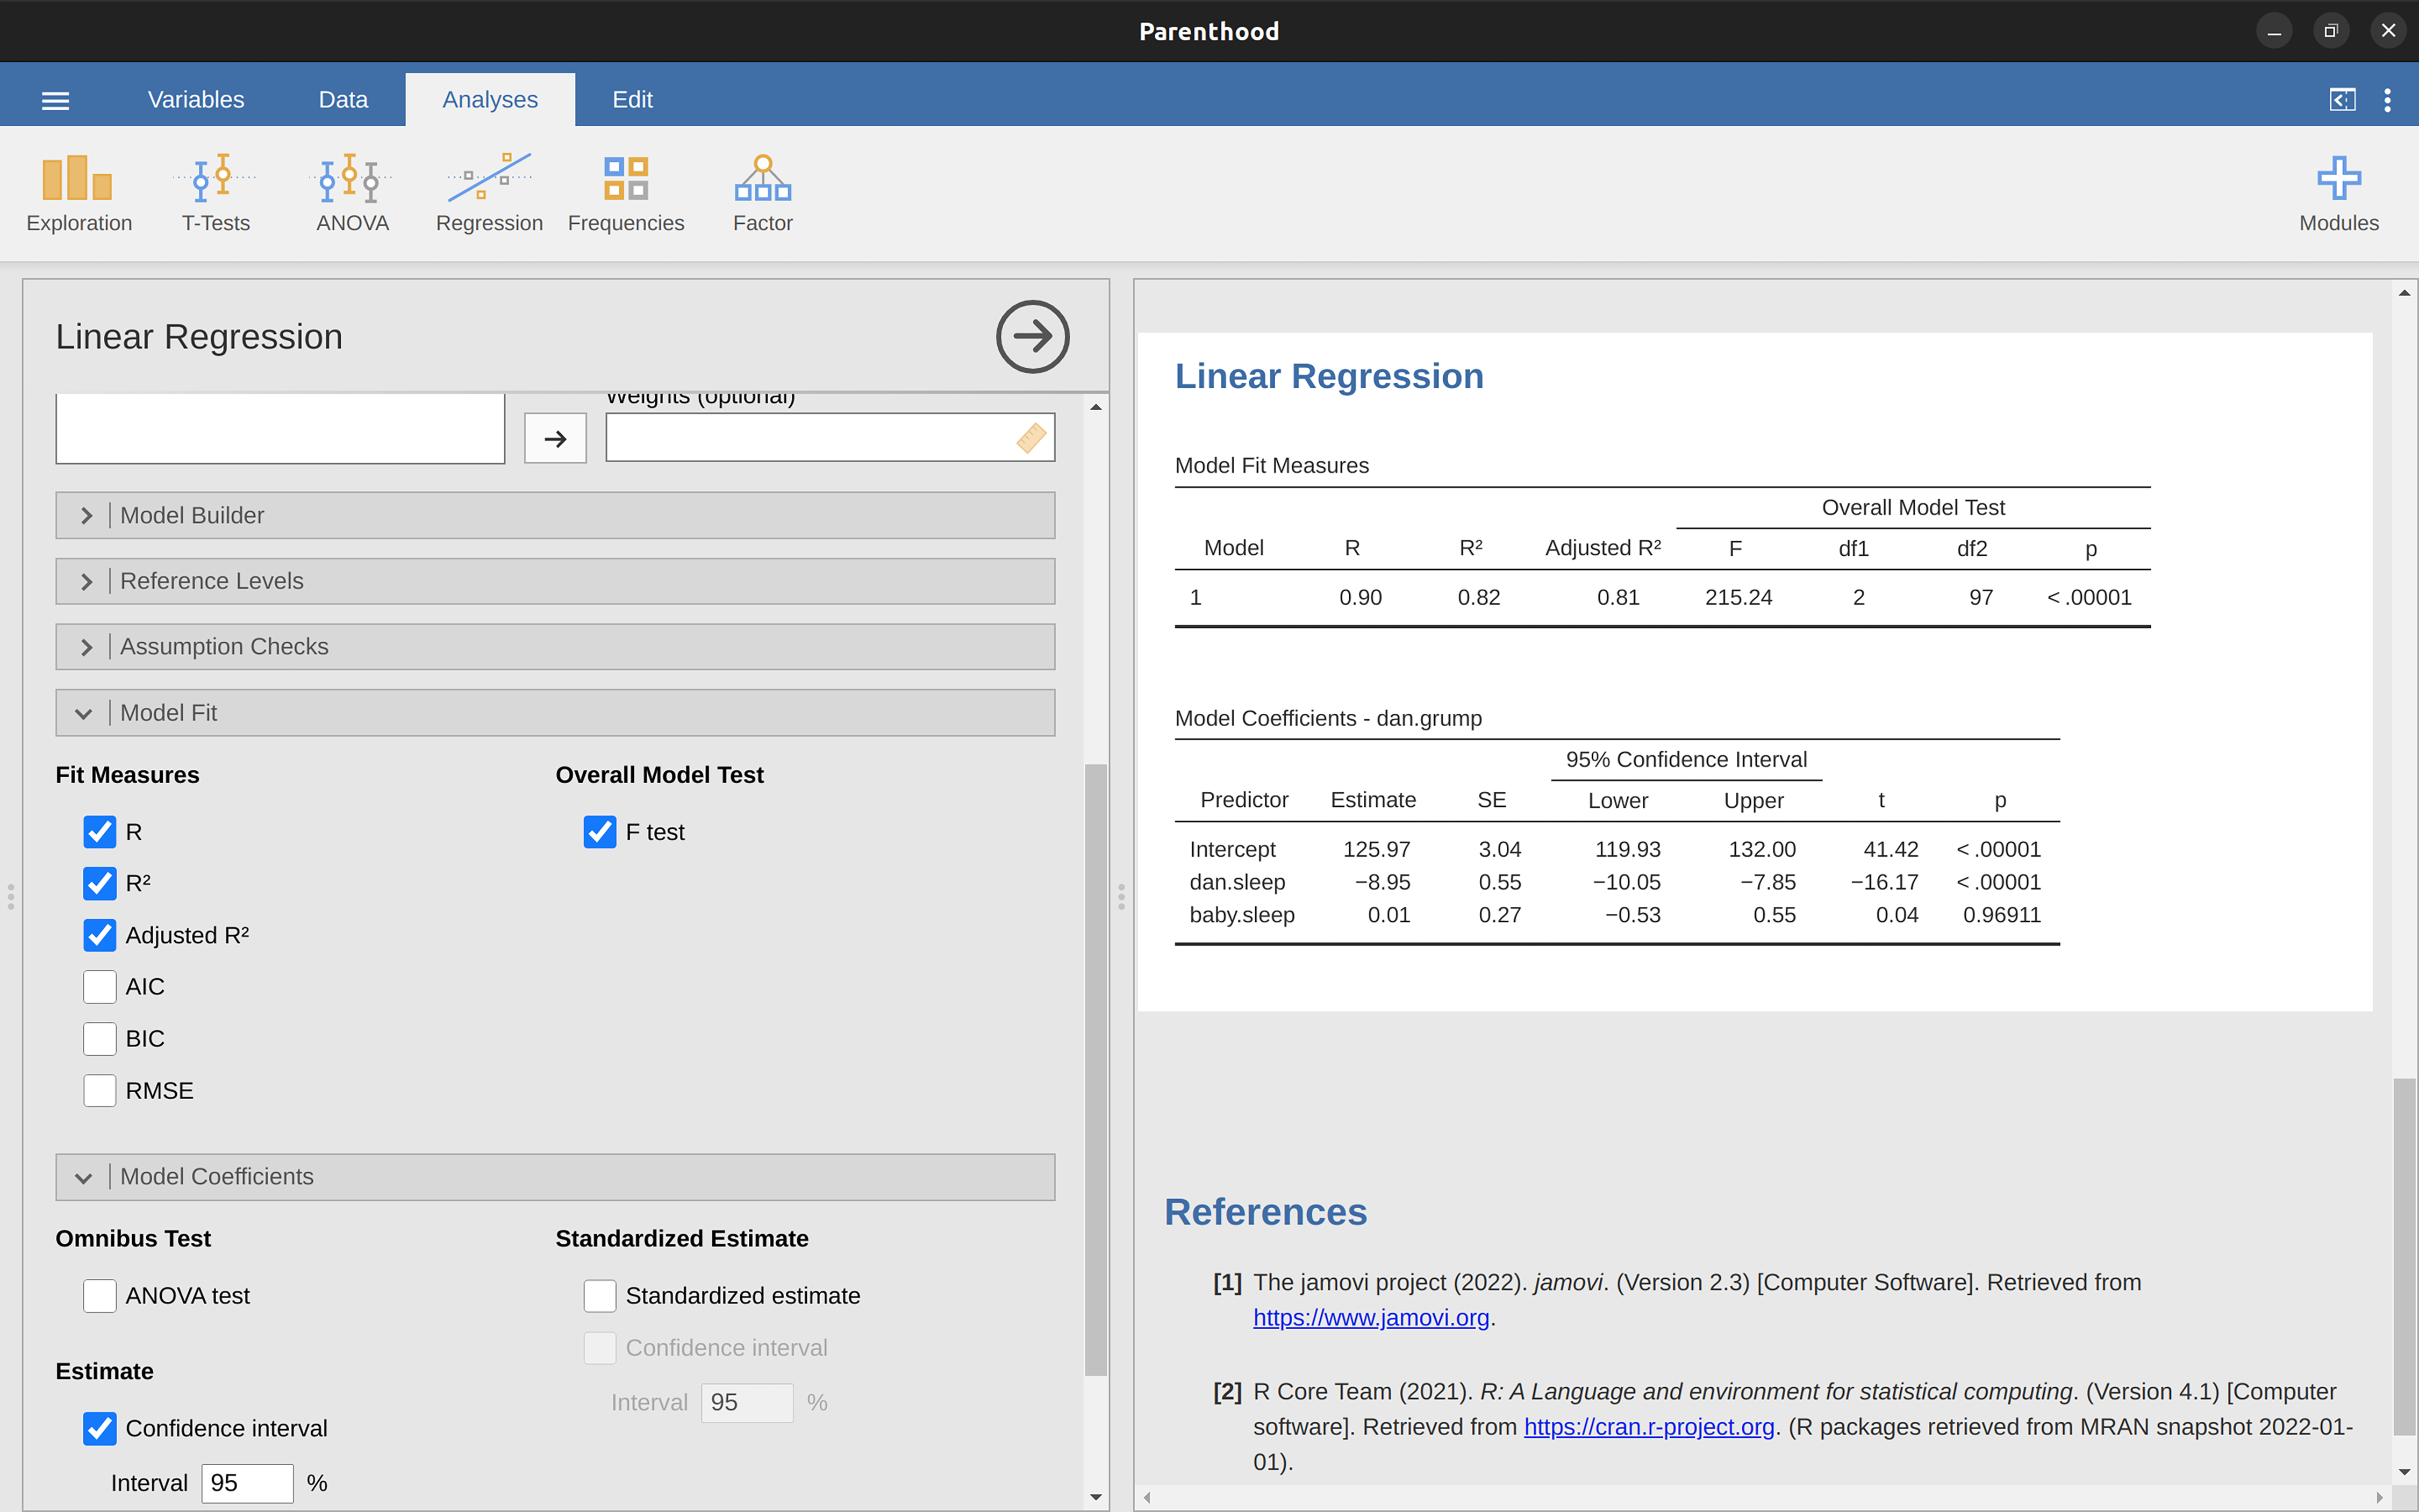
\includegraphics[width=1\textwidth,height=\textheight]{images/fig12-15.png} \hfill{}

\caption{\label{fig-fig12-15}A jamovi screenshot showing a multiple
linear regression analysis, with some useful options checked}

\end{figure}

The `Model Coefficients' at the bottom of the jamovi analysis results
shown in Figure~\ref{fig-fig12-15} provides the coefficients of the
regression model. Each row in this table refers to one of the
coefficients in the regression model. The first row is the intercept
term, and the later ones look at each of the predictors. The columns
give you all of the relevant information. The first column is the actual
estimate of \(b\) (e.g., \(125.97\) for the intercept, and -8.95 for the
dani.sleep predictor). The second column is the standard error estimate
\(\hat{\sigma}_b\). The third and fourth columns provide the lower and
upper values for the 95\% confidence interval around the \(b\) estimate
(more on this later). The fifth column gives you the \emph{t} statistic,
and it's worth noticing that in this table
\(t=\frac{\hat{b}} {se({\hat{b}})}\) every time. Finally, the last
column gives you the actual \(p\)-value for each of these
tests.\footnote{Note that, although jamovi has done multiple tests here,
  it hasn't done a Bonferroni correction or anything (see
  Chapter~\ref{sec-Comparing-several-means-one-way-ANOVA}). These are
  standard one-sample \(t\)-tests with a two-sided alternative. If you
  want to make corrections for multiple tests, you need to do that
  yourself.}

The only thing that the coefficients table itself doesn't list is the
degrees of freedom used in the \(t\)-test, which is always \(N - K - 1\)
and is listed in the table at the top of the output, labelled `Model Fit
Measures'. We can see from this table that the model performs
significantly better than you'd expect by chance
(\(F(2,97) = 215.24, p< .001\)), which isn't all that surprising: the
\(R^2 = .81\) value indicate that the regression model accounts for
\(81\%\) of the variability in the outcome measure (and \(82\%\) for the
adjusted \(R^2\) ). However, when we look back up at the \(t\)-tests for
each of the individual coefficients, we have pretty strong evidence that
the baby.sleep variable has no significant effect. All the work in this
model is being done by the dani.sleep variable. Taken together, these
results suggest that this regression model is actually the wrong model
for the data. You'd probably be better off dropping the baby.sleep
predictor entirely. In other words, the simple regression model that we
started with is the better model.

\hypertarget{regarding-regression-coefficients}{%
\section{Regarding regression
coefficients}\label{regarding-regression-coefficients}}

Before moving on to discuss the assumptions underlying linear regression
and what you can do to check if they're being met, there's two more
topics I want to briefly discuss, both of which relate to the regression
coefficients. The first thing to talk about is calculating confidence
intervals for the coefficients. After that, I'll discuss the somewhat
murky question of how to determine which predictor is most important.

\hypertarget{confidence-intervals-for-the-coefficients}{%
\subsection{Confidence intervals for the
coefficients}\label{confidence-intervals-for-the-coefficients}}

Like any population parameter, the regression coefficients \(b\) cannot
be estimated with complete precision from a sample of data; that's part
of why we need hypothesis tests. Given this, it's quite useful to be
able to report confidence intervals that capture our uncertainty about
the true value of \(b\). This is especially useful when the research
question focuses heavily on an attempt to find out how strongly variable
\(X\) is related to variable \(Y\), since in those situations the
interest is primarily in the regression weight \(b\).

{[}Additional technical detail\footnote{Fortunately, confidence
  intervals for the regression weights can be constructed in the usual
  fashion \(CI(b)=\hat{b} \pm (t_{crit} \times SE(\hat{b}))\) where
  \(se(\hat{b})\) is the standard error of the regression coefficient,
  and \(t_crit\) is the relevant critical value of the appropriate
  \emph{t} distribution. For instance, if it's a 95\% confidence
  interval that we want, then the critical value is the \(97.5\)th
  quantile of a \emph{t} distribution with \(N -K -1\) degrees of
  freedom. In other words, this is basically the same approach to
  calculating confidence intervals that we've used throughout.}{]}

In jamovi we had already specified the `95\% Confidence interval' as
shown in Figure~\ref{fig-fig12-15}, although we could easily have chosen
another value, say a `99\% Confidence interval' if that is what we
decided on.

\hypertarget{calculating-standardised-regression-coefficients}{%
\subsection{Calculating standardised regression
coefficients}\label{calculating-standardised-regression-coefficients}}

One more thing that you might want to do is to calculate
``standardised'' regression coefficients, often denoted \(\beta\). The
rationale behind standardised coefficients goes like this. In a lot of
situations, your variables are on fundamentally different scales.
Suppose, for example, my regression model aims to predict people's
\(IQ\) scores using their educational attainment (number of years of
education) and their income as predictors. Obviously, educational
attainment and income are not on the same scales. The number of years of
schooling might only vary by 10s of years, whereas income can vary by
10,000s of dollars (or more). The units of measurement have a big
influence on the regression coefficients. The \(b\) coefficients only
make sense when interpreted in light of the units, both of the predictor
variables and the outcome variable. This makes it very difficult to
compare the coefficients of different predictors. Yet there are
situations where you really do want to make comparisons between
different coefficients. Specifically, you might want some kind of
standard measure of which predictors have the strongest relationship to
the outcome. This is what \textbf{standardised coefficients} aim to do.

The basic idea is quite simple; the standardised coefficients are the
coefficients that you would have obtained if you'd converted all the
variables to \emph{z}-scores before running the regression.\footnote{Strictly,
  you standardise all the \emph{regressors}. That is, every ``thing''
  that has a regression coefficient associated with it in the model. For
  the regression models that I've talked about so far, each predictor
  variable maps onto exactly one regressor, and vice versa. However,
  that's not actually true in general and we'll see some examples of
  this later in Chapter~\ref{sec-Factorial-ANOVA}. But, for now we don't
  need to care too much about this distinction.} The idea here is that,
by converting all the predictors to \emph{z}-scores, they all go into
the regression on the same scale, thereby removing the problem of having
variables on different scales. Regardless of what the original variables
were, a \(\beta\) value of 1 means that an increase in the predictor of
1 standard deviation will produce a corresponding 1 standard deviation
increase in the outcome variable. Therefore, if variable \(A\) has a
larger absolute value of \(\beta\) than variable \(B\), it is deemed to
have a stronger relationship with the outcome. Or at least that's the
idea. It's worth being a little cautious here, since this does rely very
heavily on the assumption that ``a 1 standard deviation change'' is
fundamentally the same kind of thing for all variables. It's not always
obvious that this is true.

{[}Additional technical detail\footnote{Leaving aside the interpretation
  issues, let's look at how it's calculated. What you could do is
  standardise all the variables yourself and then run a regression, but
  there's a much simpler way to do it. As it turns out, the \(\beta\)
  coefficient for a predictor \(X\) and outcome \(Y\) has a very simple
  formula, namely \(\beta_X=b_X \times \frac{\sigma_X}{\sigma_Y}\) where
  \(\sigma_X\) is the standard deviation of the predictor, and
  \(\sigma_Y\) is the standard deviation of the outcome variable \(Y\).
  This makes matters a lot simpler.}{]}

To make things even simpler, jamovi has an option that computes the
\(\beta\) coefficients for you using the `Standardized estimate'
checkbox in the `Model Coefficients' options, see results in
Figure~\ref{fig-fig12-16}.

\begin{figure}

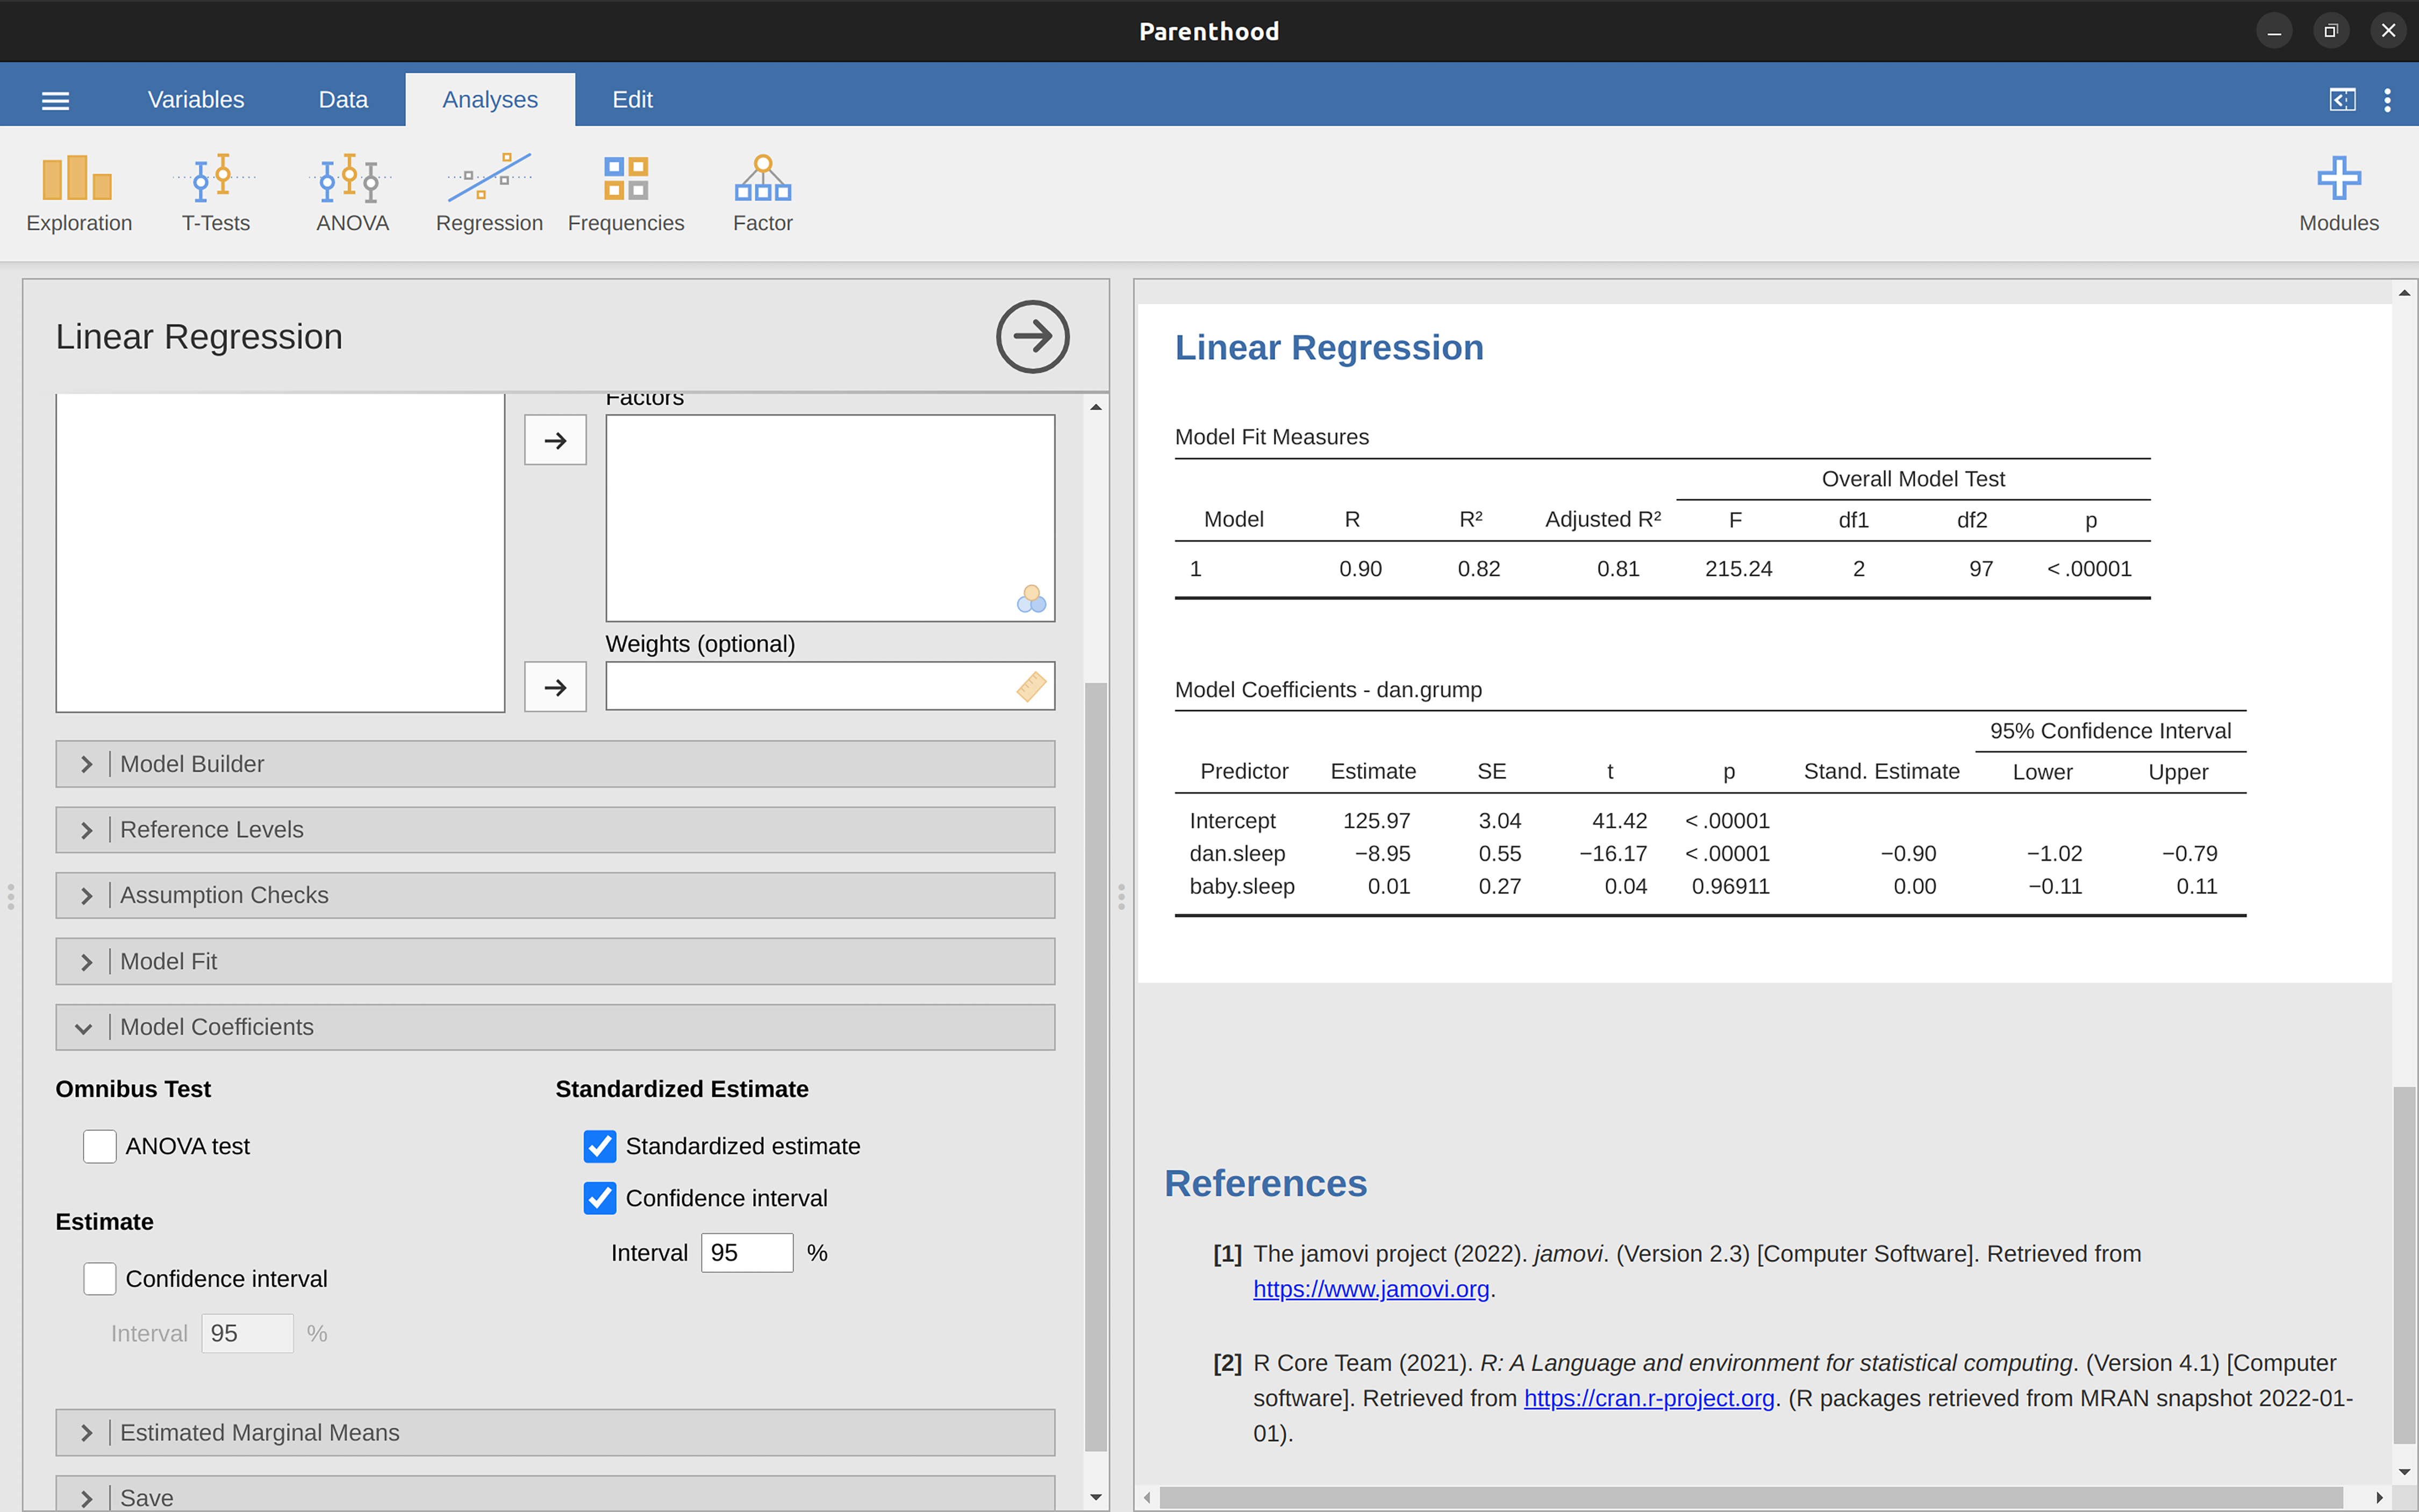
\includegraphics[width=1\textwidth,height=\textheight]{images/fig12-16.png} \hfill{}

\caption{\label{fig-fig12-16}Standardised coefficients, with 95\%
confidence intervals, for multiple linear regression}

\end{figure}

These results clearly show that the dani.sleep variable has a much
stronger effect than the baby.sleep variable. However, this is a perfect
example of a situation where it would probably make sense to use the
original coefficients b rather than the standardised coefficients
\(\beta\). After all, my sleep and the baby's sleep are already on the
same scale: number of hours slept. Why complicate matters by converting
these to \emph{z}-scores?

\hypertarget{assumptions-of-regression}{%
\section{Assumptions of regression}\label{assumptions-of-regression}}

The linear regression model that I've been discussing relies on several
assumptions. In \protect\hyperlink{sec-Model-checking}{Model checking}
we'll talk a lot more about how to check that these assumptions are
being met, but first let's have a look at each of them.

\begin{itemize}
\tightlist
\item
  \textbf{L}inearity. A pretty fundamental assumption of the linear
  regression model is that the relationship between \(X\) and \(Y\)
  actually is linear! Regardless of whether it's a simple regression or
  a multiple regression, we assume that the relationships involved are
  linear.
\item
  \textbf{I}ndependence: residuals are independent of each other. This
  is really just a ``catch all'' assumption, to the effect that
  ``there's nothing else funny going on in the residuals''. If there is
  something weird (e.g., the residuals all depend heavily on some other
  unmeasured variable) going on, it might screw things up. Independence
  isn't something that you can check directly and specifically with
  diagnostic tools, but if your regression diagnostics are messed up
  then think carefully about the independence of your observations and
  residuals.
\item
  \textbf{N}ormality. Like many of the models in statistics, basic
  simple or multiple linear regression relies on an assumption of
  normality. Specifically, it assumes that the residuals are normally
  distributed. It's actually okay if the predictors \(X\) and the
  outcome \(Y\) variables are non-normal, so long as the residuals
  \(\epsilon\) are normal. See the
  \protect\hyperlink{sec-Checking-the-normality-of-the-residuals}{Checking
  the normality of the residuals} section.
\item
  \textbf{E}quality (or ``homogeneity'') of variance. Strictly speaking,
  the regression model assumes that each residual \(\epsilon_i\) is
  generated from a normal distribution with mean 0, and (more
  importantly for the current purposes) with a standard deviation
  \(\sigma\) that is the same for every single residual. In practice,
  it's impossible to test the assumption that every residual is
  identically distributed. Instead, what we care about is that the
  standard deviation of the residual is the same for all values of
  \(\hat{Y}\), and (if we're being especially diligent) all values of
  every predictor \(X\) in the model.
\end{itemize}

So, we have four main assumptions for linear regression (that neatly
form the acronym \textbf{LINE}). And there are also a couple of other
things we should also check for:

\begin{itemize}
\tightlist
\item
  Uncorrelated predictors. The idea here is that, in a multiple
  regression model, you don't want your predictors to be too strongly
  correlated with each other. This isn't ``technically'' an assumption
  of the regression model, but in practice it's required. Predictors
  that are too strongly correlated with each other (referred to as
  ``collinearity'') can cause problems when evaluating the model. See
  \protect\hyperlink{checking-for-collinearity}{Checking for
  collinearity} section.
\item
  No ``bad'' outliers. Again, not actually a technical assumption of the
  model (or rather, it's sort of implied by all the others), but there
  is an implicit assumption that your regression model isn't being too
  strongly influenced by one or two anomalous data points because this
  raises questions about the adequacy of the model and the
  trustworthiness of the data in some cases. See the section on
  \protect\hyperlink{outliers-and-anomalous-data}{Outliers and anomalous
  data}.
\end{itemize}

\hypertarget{sec-Model-checking}{%
\section{Model checking}\label{sec-Model-checking}}

The main focus of this section is \textbf{regression diagnostics}, a
term that refers to the art of checking that the assumptions of your
regression model have been met, figuring out how to fix the model if the
assumptions are violated, and generally to check that nothing ``funny''
is going on. I refer to this as the ``art'' of model checking with good
reason. It's not easy, and while there are a lot of easily available
tools that you can use to diagnose and maybe even cure the problems that
affect your model (if there are any, that is!), you really do need to
exercise a certain amount of judgement when doing this.

In this section I describe several different things you can do to check
that your regression model is doing what it's supposed to. It doesn't
cover the full space of things you could do, but it's still much more
detailed than what is often done in practice -- unfortunately! But it's
important that you get a sense of what tools are at your disposal, so
I'll try to introduce a bunch of them here. Finally, I should note that
this section draws quite heavily from Fox \& Weisberg (2011), the book
associated with the ``car'' package that is used to conduct regression
analysis in \(R\). The ``car'' package is notable for providing some
excellent tools for regression diagnostics, and the book itself talks
about them in an admirably clear fashion. I don't want to sound too
gushy about it, but I do think that Fox \& Weisberg (2011) is well worth
reading, even if some of the advanced diagnostic techniques are only
available in ``R'' and not jamovi.

\hypertarget{three-kinds-of-residuals}{%
\subsection{Three kinds of residuals}\label{three-kinds-of-residuals}}

The majority of regression diagnostics revolve around looking at the
residuals, and there are several different kinds of residual that we
might consider. In particular, the following three kinds of residuals
are referred to in this section: ``ordinary residuals'', ``standardised
residuals'', and ``Studentised residuals''. There is a fourth kind that
you'll see referred to in some of the Figures, and that's the ``Pearson
residual''. However, for the models that we're talking about in this
chapter the Pearson residual is identical to the ordinary residual.

The first and simplest kind of residuals that we care about are
\textbf{ordinary residuals}. These are the actual raw residuals that
I've been talking about throughout this chapter so far. The ordinary
residual is just the difference between the predicted value
\(\hat{Y}_i\) and the observed value \(Y_i\). I've been using the
notation \(\epsilon_i\) to refer to the i-th ordinary residual and so,
with this in mind, we have the very simple equation

\[\epsilon_i=Y_i-\hat{Y_i}\]

This is of course what we saw earlier, and unless I specifically refer
to some other kind of residual, this is the one I'm talking about. So
there's nothing new here. I just wanted to repeat myself. One drawback
to using ordinary residuals is that they're always on a different scale,
depending on what the outcome variable is and how good the regression
model is. That is, unless you've decided to run a regression model
without an intercept term, the ordinary residuals will have mean 0 but
the variance is different for every regression. In a lot of contexts,
especially where you're only interested in the pattern of the residuals
and not their actual values, it's convenient to estimate the
\textbf{standardised residuals}, which are normalised in such a way as
to have a standard deviation of 1.

{[}Additional technical detail\footnote{The way we calculate these is to
  divide the ordinary residual by an estimate of the (population)
  standard deviation of these residuals. For technical reasons, the
  formula for this is
  \[\epsilon_i^{'}=\frac{\epsilon_i}{\hat{\sigma}\sqrt{1-h_i}}\] where
  \(\hat{\sigma}\) in this context is the estimated population standard
  deviation of the ordinary residuals, and \(h_i\) is the ``hat value''
  of the \(i\)th observation. I haven't explained hat values to you yet,
  so this won't make a lot of sense. For now, it's enough to interpret
  the standardised residuals as if we'd converted the ordinary residuals
  to \emph{z}-scores.}{]}

The third kind of residuals are \textbf{Studentised residuals} (also
called ``jackknifed residuals'') and they're even fancier than
standardised residuals. Again, the idea is to take the ordinary residual
and divide it by some quantity in order to estimate some standardised
notion of the residual.\footnote{The formula for doing the calculations
  this time is subtly different
  \(\epsilon _i^*=\frac{\epsilon_i}{\hat{\sigma}_{(-i)}\sqrt{1-h_i}}\)
  Notice that our estimate of the standard deviation here is written
  \(\hat{\sigma}_{(-i)}\). What this corresponds to is the estimate of
  the residual standard deviation that you would have obtained if you
  just deleted the \(i\)th observation from the data set. This sounds
  like the sort of thing that would be a nightmare to calculate, since
  it seems to be saying that you have to run \(N\) new regression models
  (even a modern computer might grumble a bit at that, especially if
  you've got a large data set). Fortunately, this standard deviation
  estimate is actually given by the following equation:
  \(\hat{\sigma}_{(-i)}= \hat{\sigma}\sqrt{\frac{N-K-1-{\epsilon_i^{'}}^2}{N-K-2}}\).}

Before moving on, I should point out that you don't often need to obtain
these residuals yourself, even though they are at the heart of almost
all regression diagnostics. Most of the time the various options that
provide the diagnostics, or assumption checks, will take care of these
calculations for you. Even so, it's always nice to know how to actually
get hold of these things yourself in case you ever need to do something
non-standard.

\hypertarget{checking-the-linearity-of-the-relationship}{%
\subsection{Checking the linearity of the
relationship}\label{checking-the-linearity-of-the-relationship}}

We should check for the linearity of the relationships between the
predictors and the outcomes. There's a few different things that you
might want to do in order to check this. Firstly, it never hurts to just
plot the relationship between the predicted values \(\hat{Y}_i\) and the
observed values \(Y_i\) for the outcome variable, as illustrated in
Figure~\ref{fig-fig12-17}. To draw this in jamovi we saved the predicted
values to the dataset, and then drew a scatterplot of the observed
against the predicted (fitted) values. This gives you a kind of ``big
picture view'' -- if this plot looks approximately linear, then we're
probably not doing too badly (though that's not to say that there aren't
problems). However, if you can see big departures from linearity here,
then it strongly suggests that you need to make some changes.

\begin{figure}

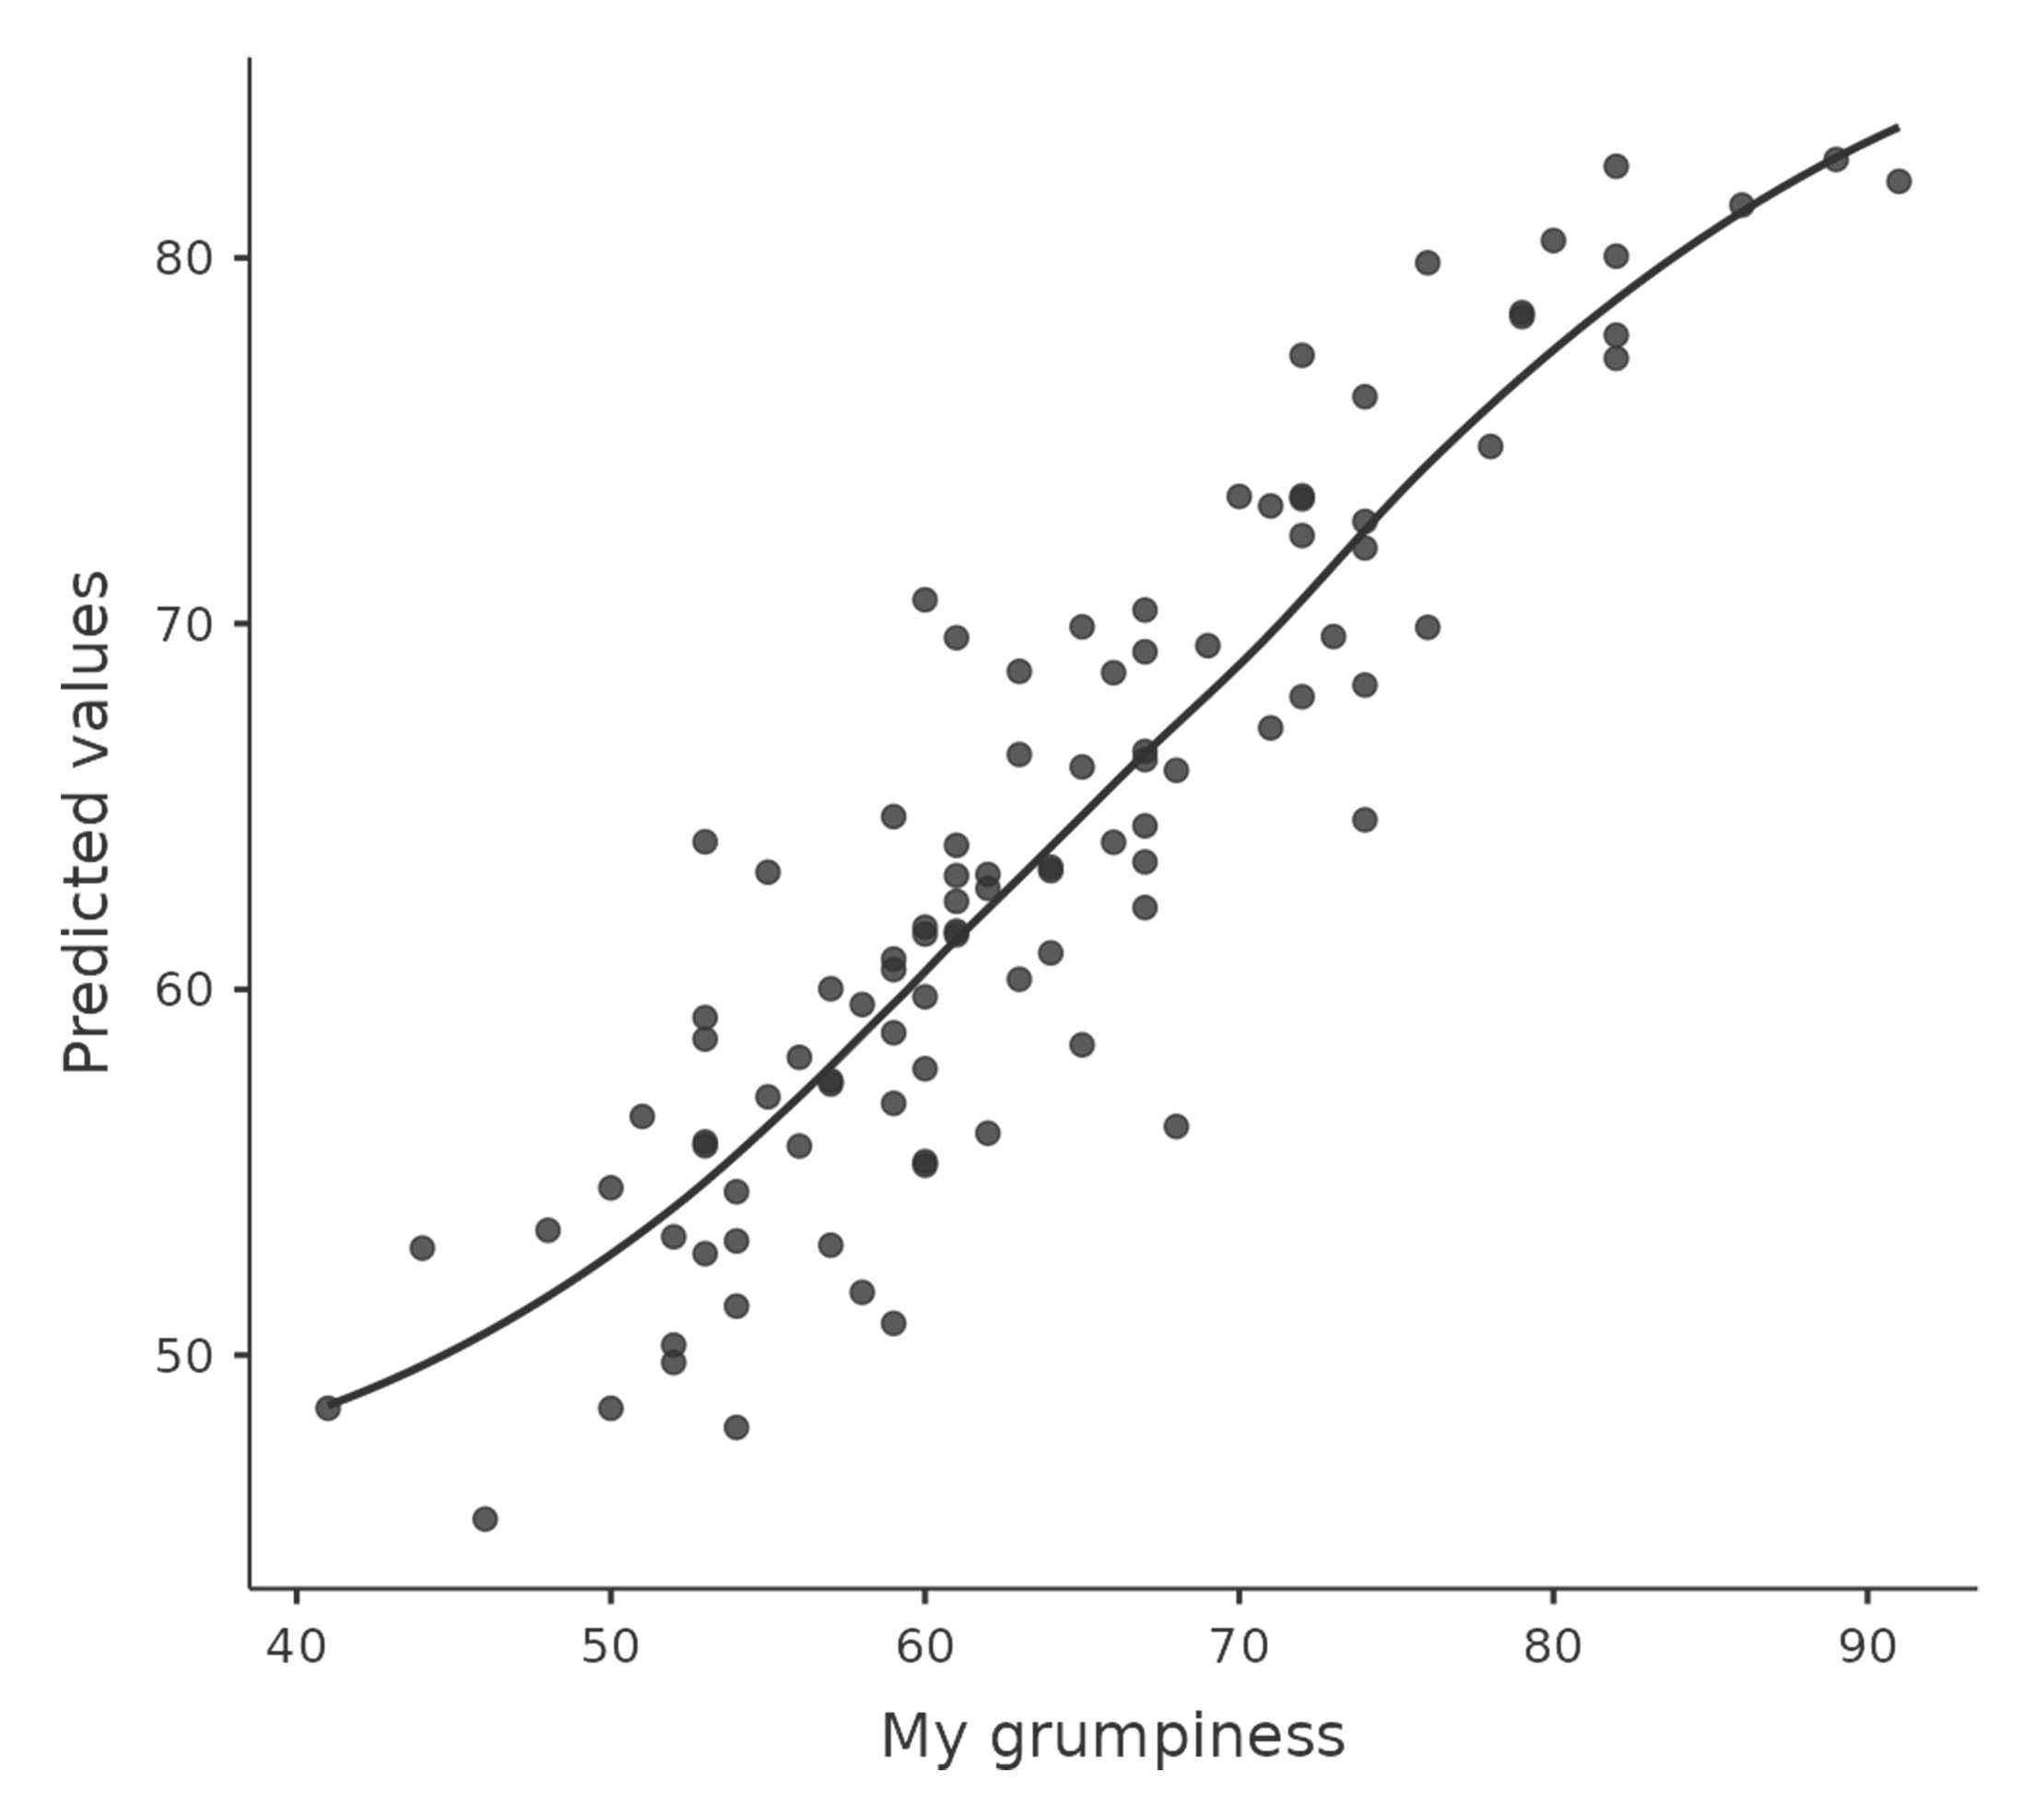
\includegraphics[width=1\textwidth,height=\textheight]{images/fig12-17.png} \hfill{}

\caption{\label{fig-fig12-17}jamovi plot of the predicted values against
the observed values of the outcome variable. A straight(-ish) line is
what we are hoping to see here. This looks pretty good, suggesting that
there is nothing grossly wrong}

\end{figure}

In any case, in order to get a more detailed picture it's often more
informative to look at the relationship between the predicted values and
the residuals themselves. Again, in jamovi you can save the residuals to
the dataset and then draw a scatterplot of the predicted values against
the residual values, as in Figure~\ref{fig-fig12-18}. As you can see,
not only does it draw the scatterplot showing the predicted value
against the residuals, you can also plot a line through the data that
shows the relationship between the two. Ideally, this should be a
straight, perfectly horizontal line. In practice, we're looking for a
reasonably straight or flat line. This is a matter of judgement.

\begin{figure}

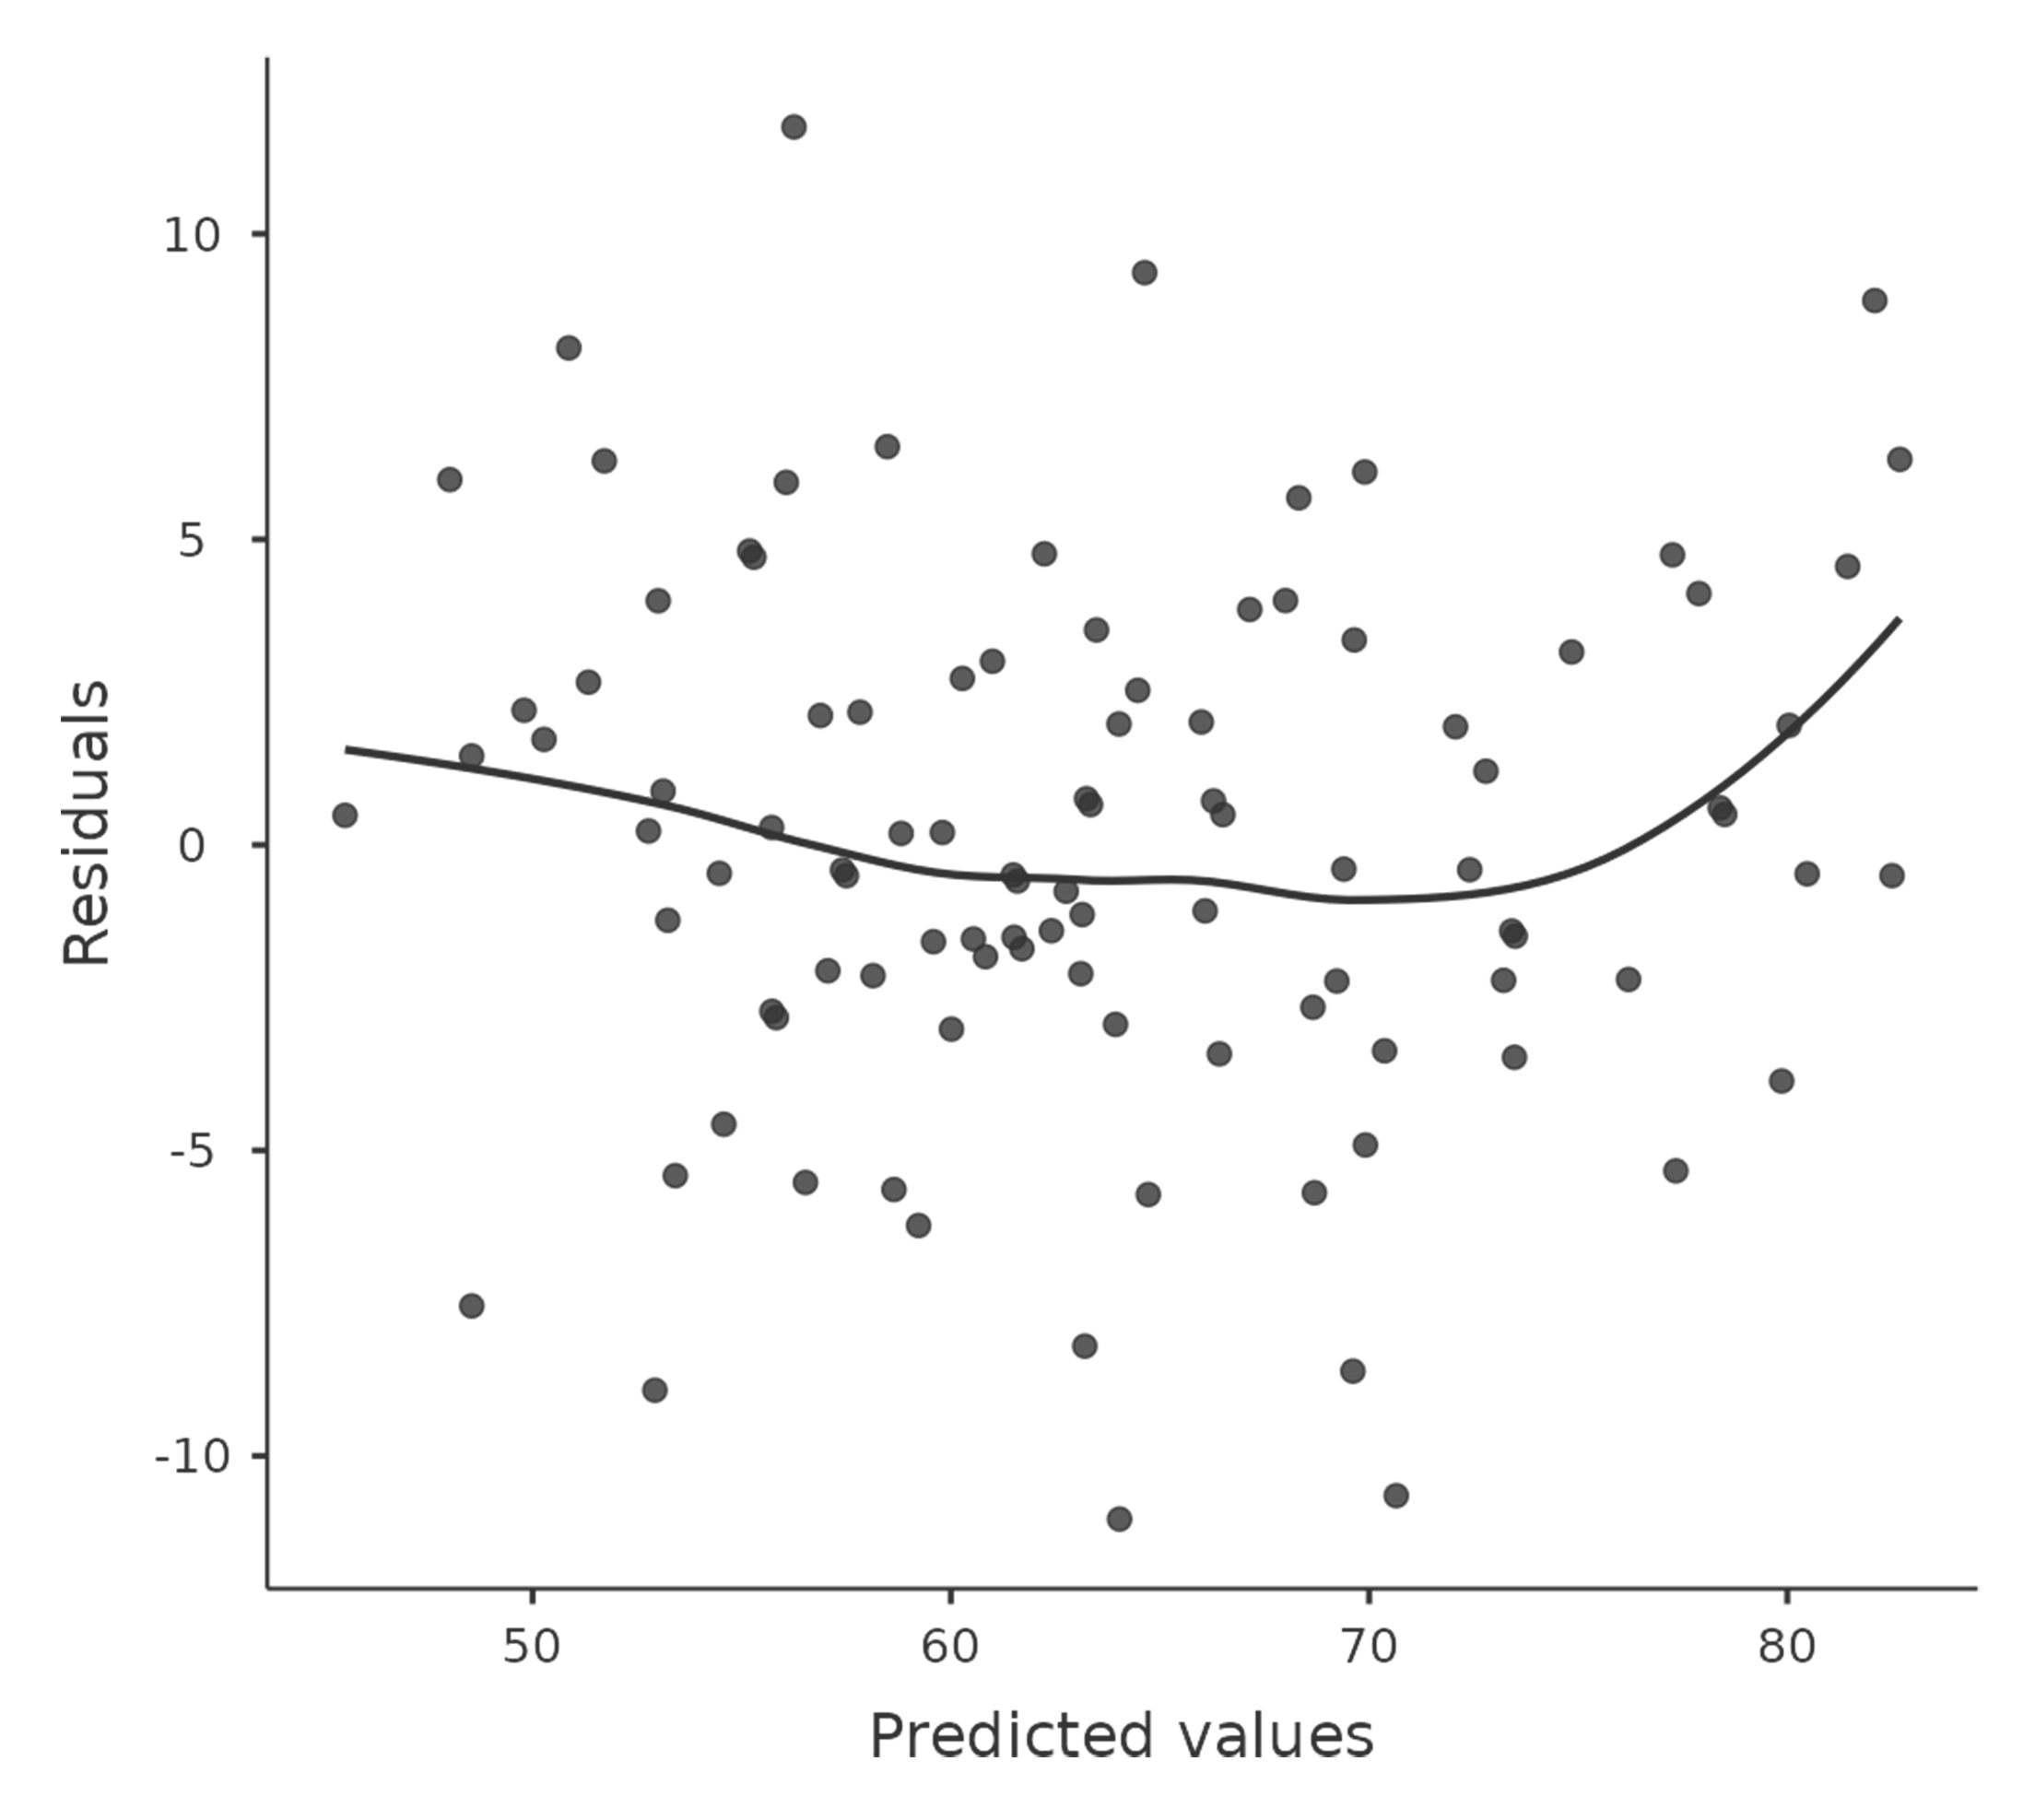
\includegraphics[width=1\textwidth,height=\textheight]{images/fig12-18.png} \hfill{}

\caption{\label{fig-fig12-18}jamovi plot of the predicted values against
the residuals, with a line showing the relationship between the two. If
this is horizontal and straight(-ish), then we can feel reasonably
confident that the ``average residual'' for all ``predicted values'' is
more or less the same.}

\end{figure}

Somewhat more advanced versions of the same plot is produced by checking
`Residuals plots' in the regression analysis `Assumption checks' options
in jamovi. These are useful not only for checking linearity, but also
for checking normality and equality of variance assumptions, and we look
at these in more detail in
Section~\ref{sec-Checking-the-normality-of-the-residuals}. This option
not only draws plots comparing the predicted values to the residuals, it
does so for each individual predictor.

\hypertarget{sec-Checking-the-normality-of-the-residuals}{%
\subsection{Checking the normality of the
residuals}\label{sec-Checking-the-normality-of-the-residuals}}

Like many of the statistical tools we've discussed in this book,
regression models rely on a normality assumption. In this case, we
assume that the residuals are normally distributed. The first thing we
can do is draw a QQ-plot via the `Assumption Checks' - `Assumption
Checks' - `Q-Q plot of residuals' option. The output is shown in
Figure~\ref{fig-fig12-19}, showing the standardised residuals plotted as
a function of their theoretical quantiles according to the regression
model.

\begin{figure}

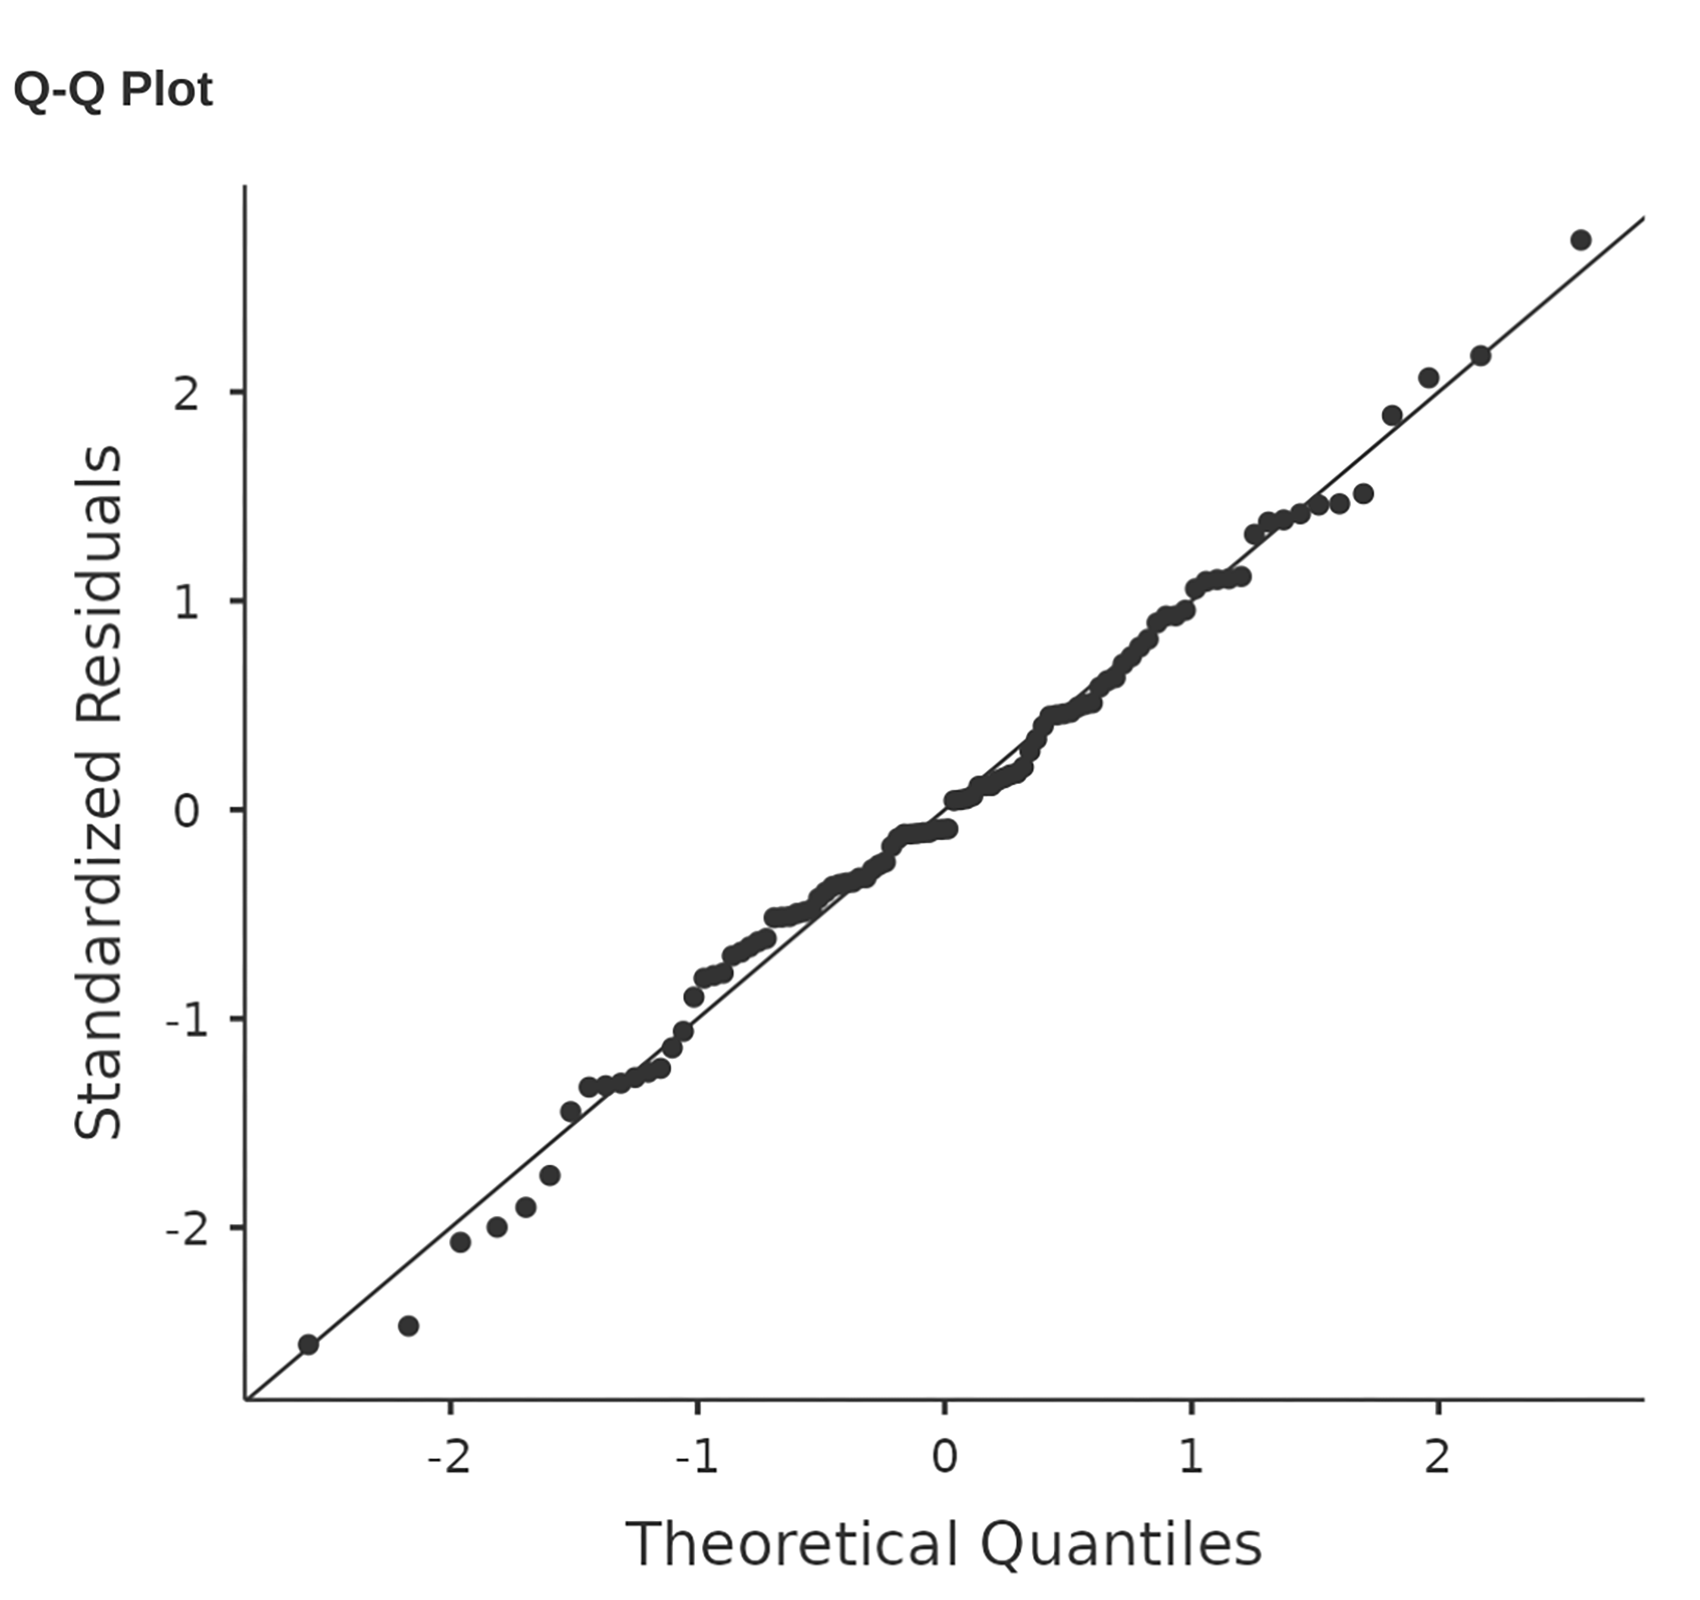
\includegraphics[width=1\textwidth,height=\textheight]{images/fig12-19.png} \hfill{}

\caption{\label{fig-fig12-19}Plot of the theoretical quantiles according
to the model, against the quantiles of the standardised residuals,
produced in jamovi}

\end{figure}

Another thing we should check is the relationship between the predicted
(fitted) values and the residuals themselves. We can get jamovi to do
this using the `Residuals Plots' option, which provides a scatterplot
for each predictor variable, the outcome variable, and the predicted
values against residuals, see Figure~\ref{fig-fig12-20}. In these plots
we are looking for a fairly uniform distribution of dots, with no clear
bunching or patterning of the dots. Looking at these plots, there is
nothing particularly worrying as the dots are fairly evenly spread
across the whole plot. There may be a little bit of non-uniformity in
plot (b), but it is not a strong deviation and probably not worth
worrying about.

\begin{figure}

\begin{minipage}[t]{\linewidth}

{\centering 

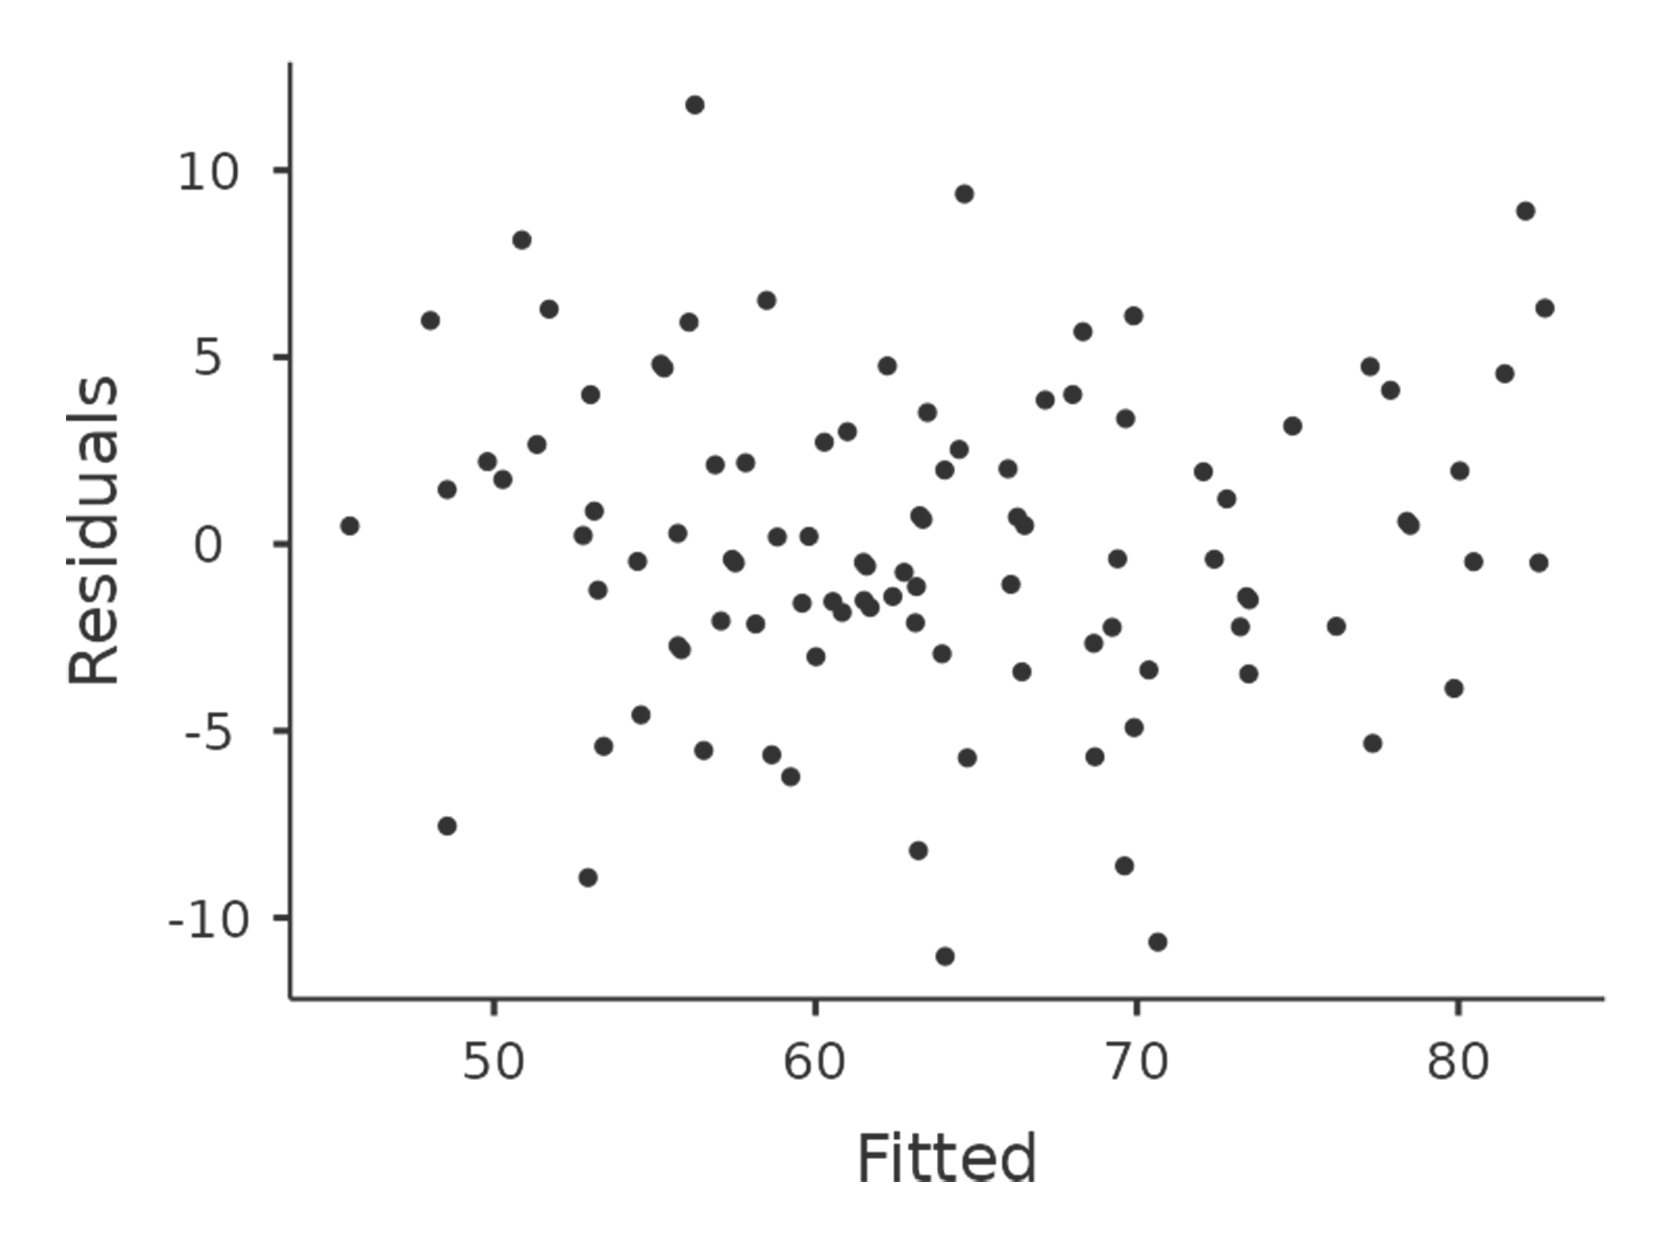
\includegraphics[width=0.45\textwidth,height=\textheight]{images/fig12-20a.png}
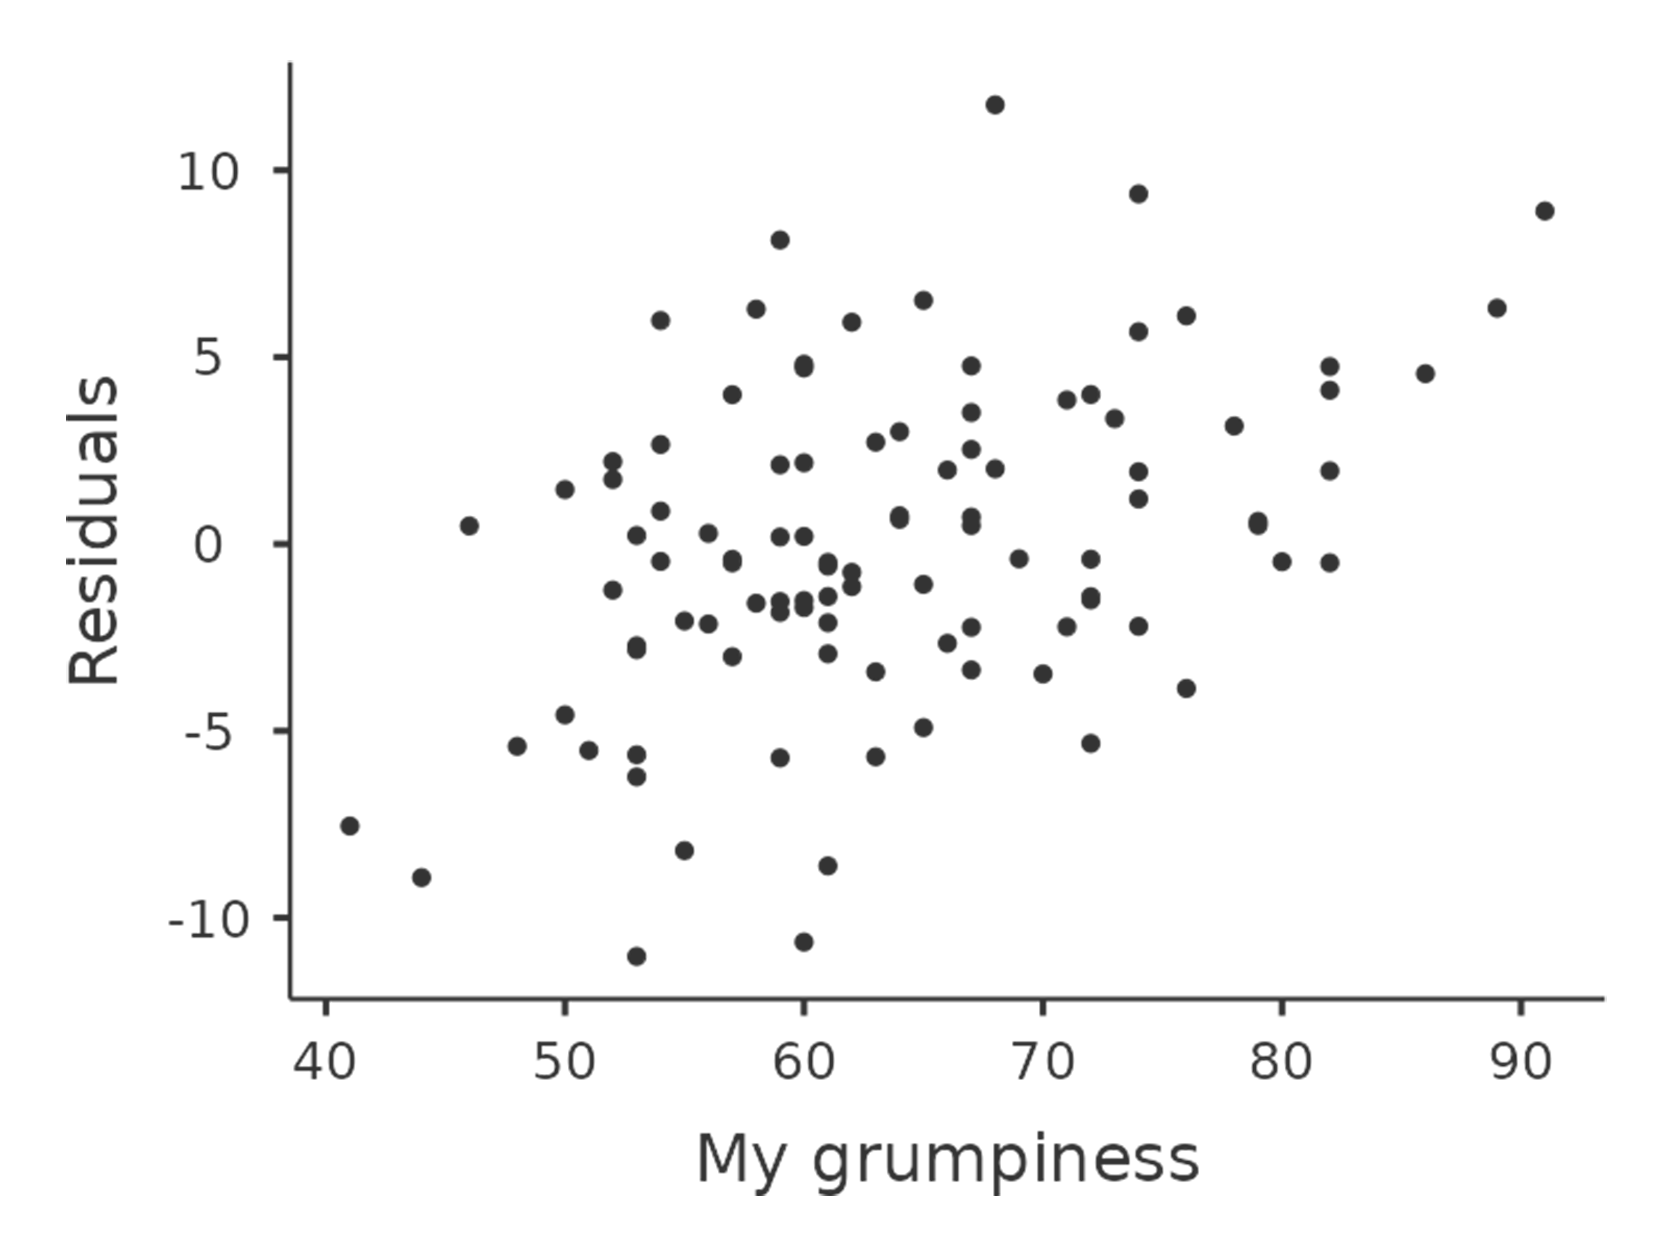
\includegraphics[width=0.45\textwidth,height=\textheight]{images/fig12-20b.png}
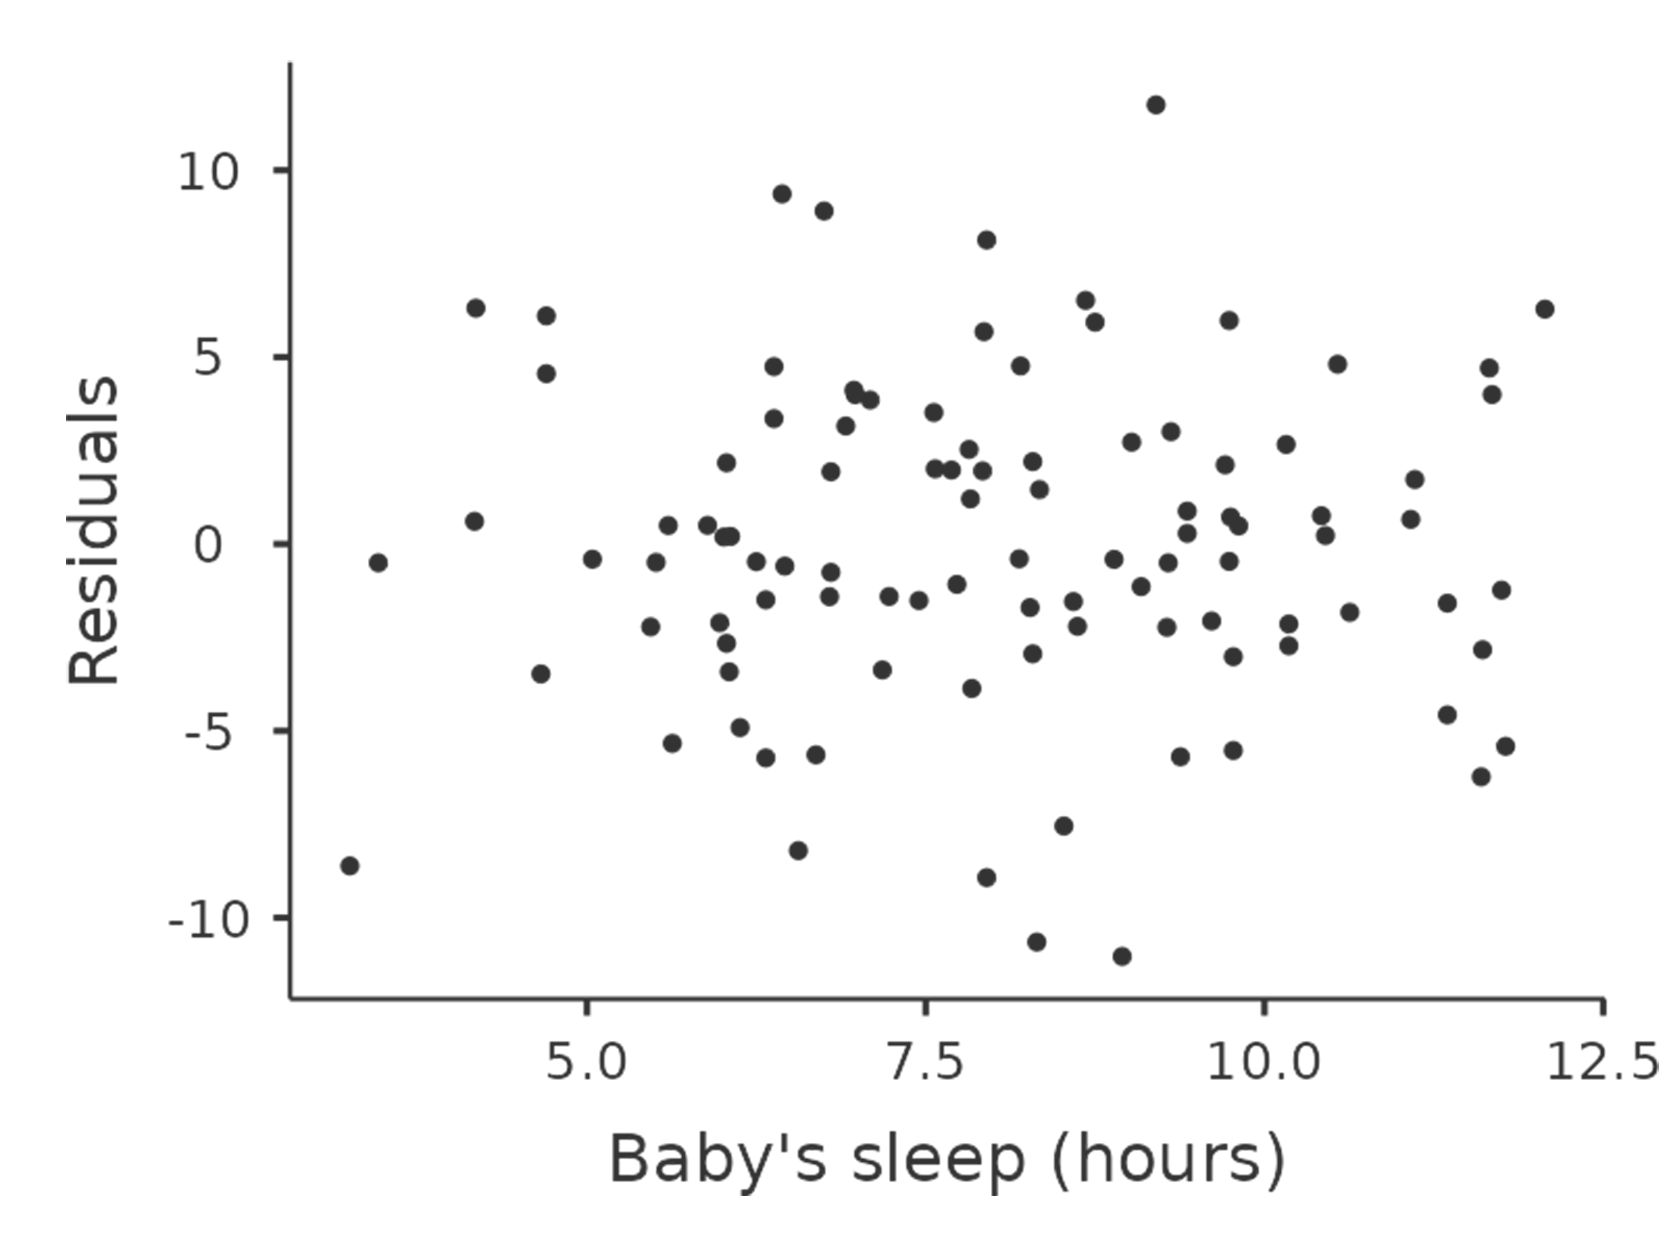
\includegraphics[width=0.45\textwidth,height=\textheight]{images/fig12-20c.png}

\includegraphics[width=0.45\textwidth,height=\textheight]{images/fig12-20d.png}

}

\end{minipage}%

\caption{\label{fig-fig12-20}Residuals plots produced in jamovi}

\end{figure}

If we were worried, then in a lot of cases the solution to this problem
(and many others) is to transform one or more of the variables. We
discussed the basics of variable transformation in
\textbf{?@sec-Transforming-and-recoding-a-variable}, but I do want to
make special note of one additional possibility that I didn't explain
fully earlier: the Box-Cox transform. The Box-Cox function is a fairly
simple one and it's very widely used.\footnote{\(f(x,\lambda)=\frac{x^{\lambda}-1}{\lambda}\)
  for all values of \(\lambda\) except \(\lambda = 0\). When
  \(\lambda = 0\) we just take the natural logarithm (i.e., ln(\(x\)).}

You can calculate it using the BOXCOX function in the `Compute'
variables screen in jamovi.

\hypertarget{checking-equality-of-variance}{%
\subsection{Checking equality of
variance}\label{checking-equality-of-variance}}

The regression models that we've talked about all make an equality
(i.e.homogeneity) of variance assumption: the variance of the residuals
is assumed to be constant. To plot this in jamovi first we need to
calculate the square root of the (absolute) size of the
residual\footnote{In jamovi, you can compute this new variable using the
  formula `SQRT(ABS(Residuals))'.} and then plot this against the
predicted values, as in Figure~\ref{fig-fig12-21}. Note that this plot
actually uses the standardised residuals rather than the raw ones, but
it's immaterial from our point of view. What we're looking to see here
is a straight, horizontal line running through the middle of the
plot.\footnote{It's a bit beyond the scope of this chapter to talk about
  how to deal with violations of homogeneity of variance, but I'll give
  you a quick sense of what you need to consider. The \textbf{main}
  thing to worry about, if homogeneity of variance is violated, is that
  the standard error estimates associated with the regression
  coefficients are no longer entirely reliable, and so your \(t\)-tests
  for the coefficients aren't quite right either. A simple fix to the
  problem is to make use of a ``heteroscedasticity corrected covariance
  matrix'' when estimating the standard errors. These are often called
  \textbf{\emph{sandwich estimators}}, and these can be estimated in
  \(R\) (but not directly in jamovi).}

\begin{figure}

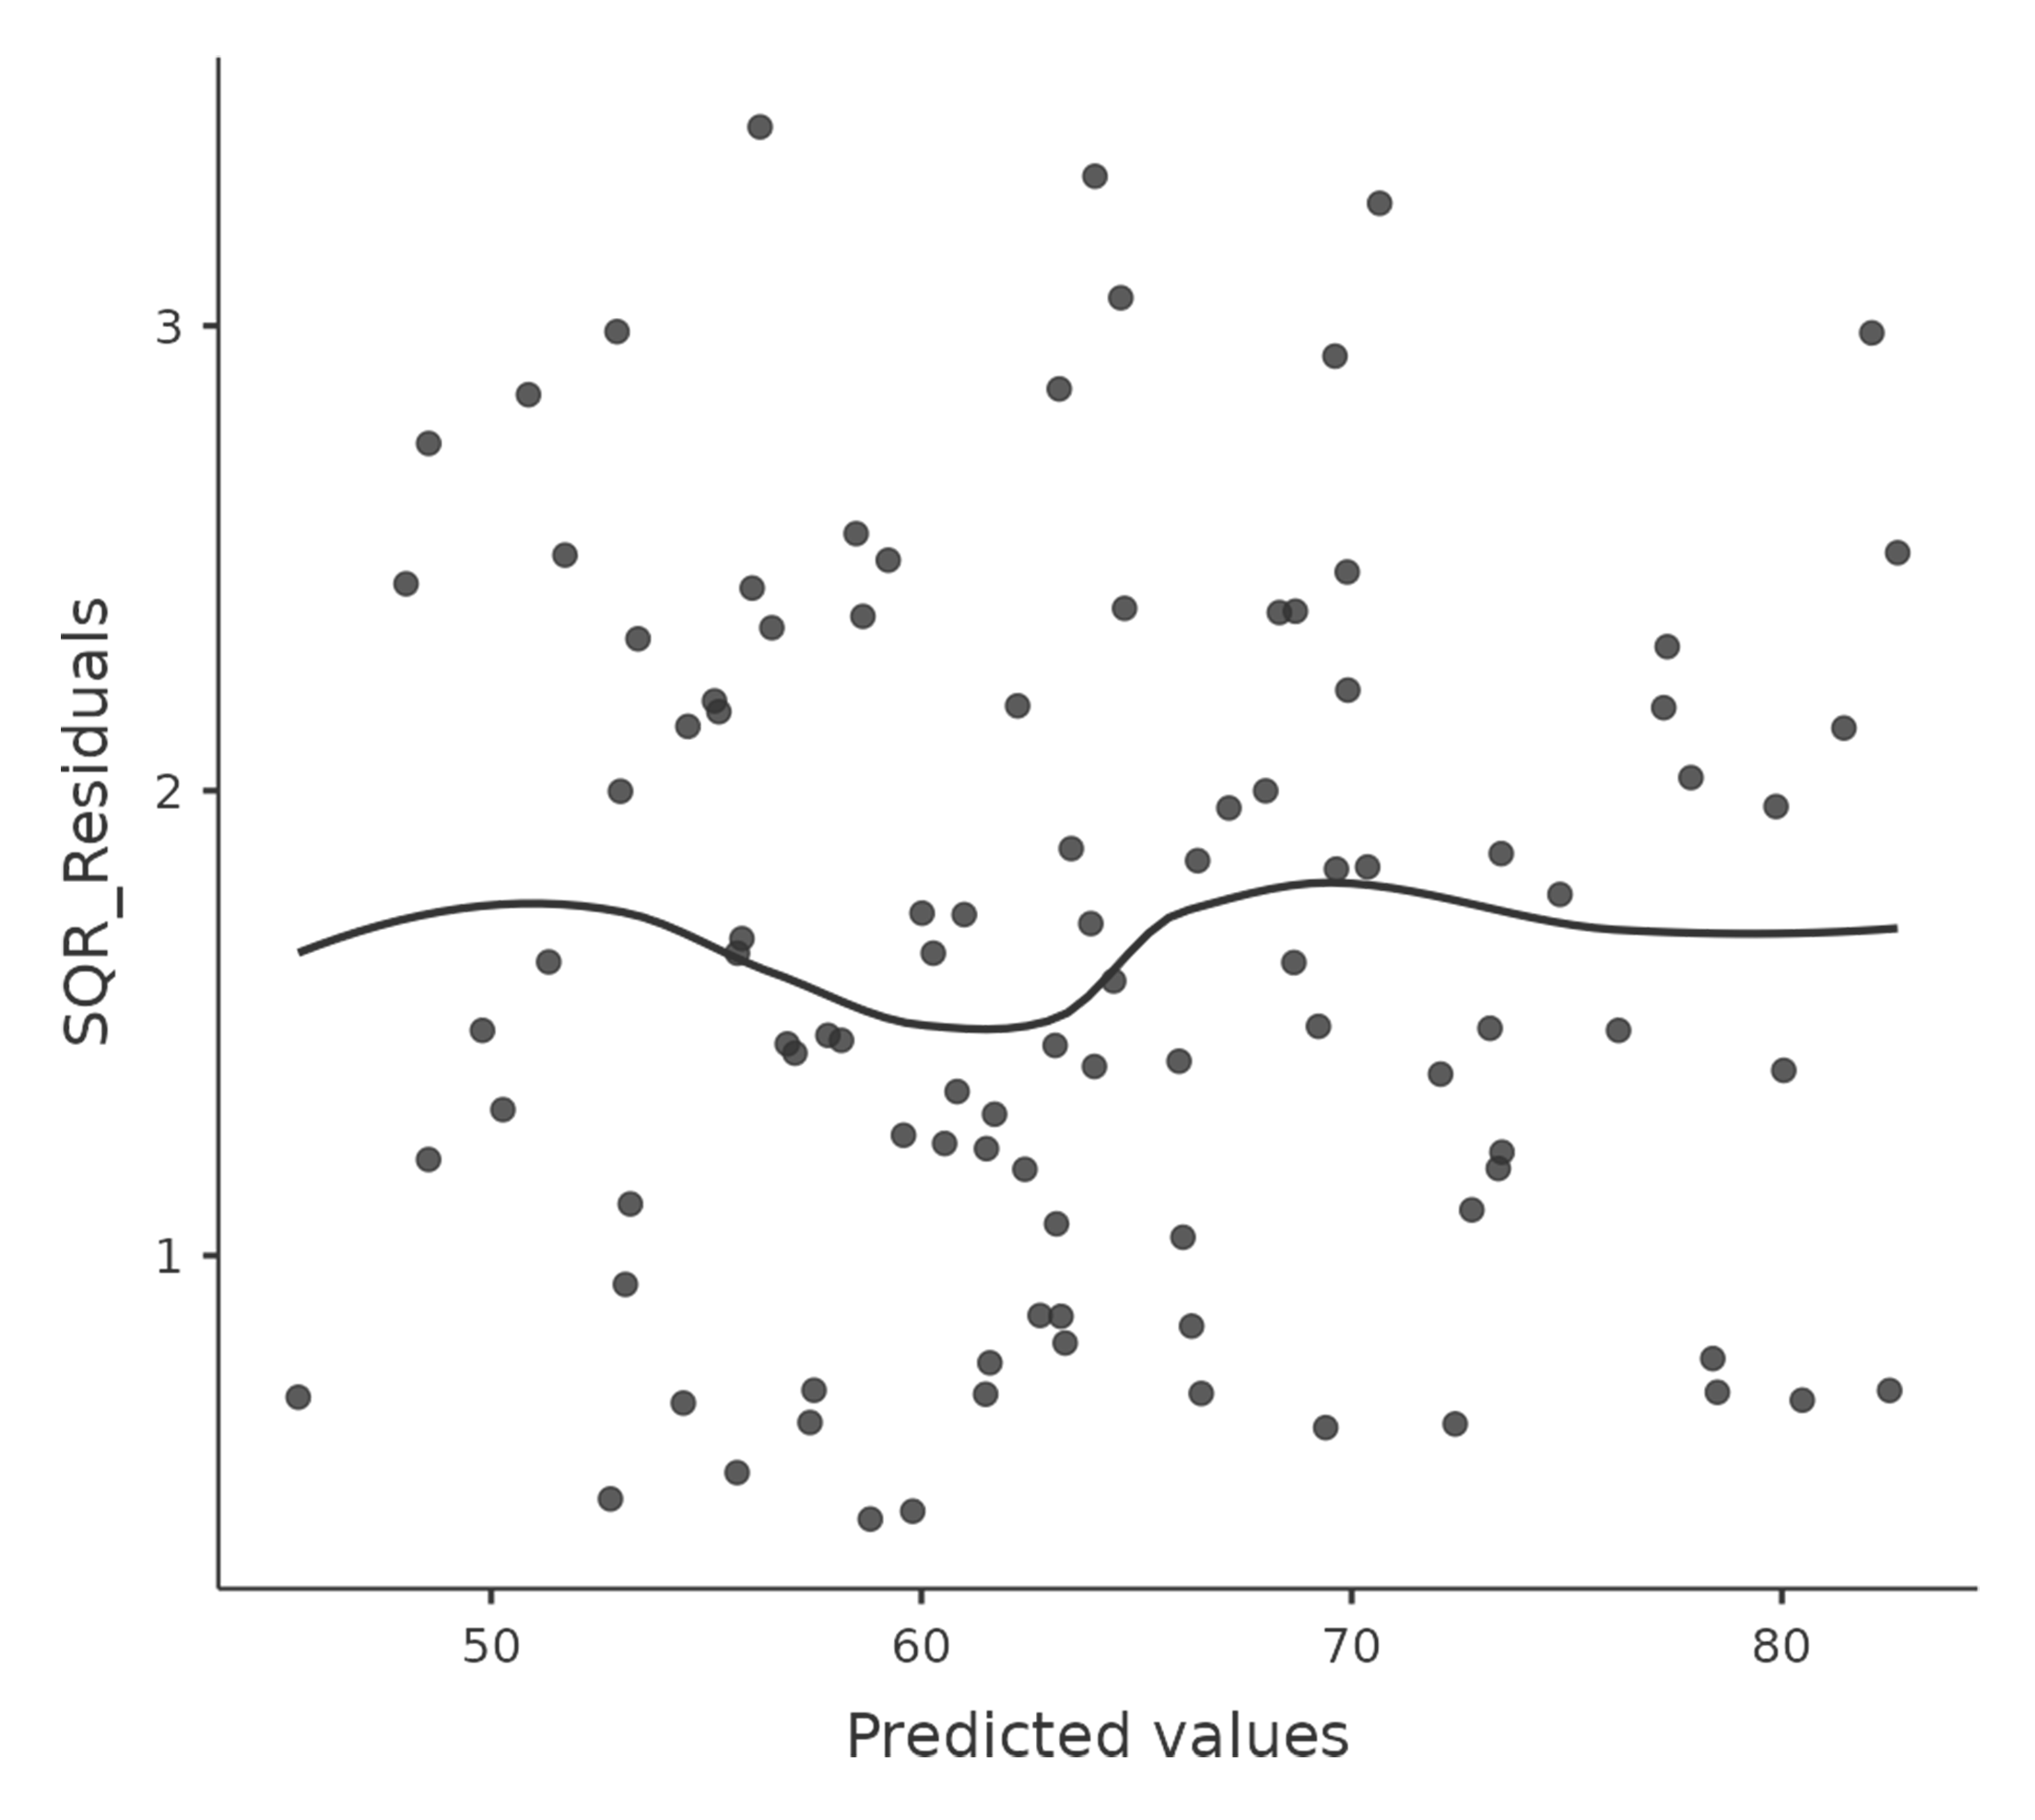
\includegraphics[width=1\textwidth,height=\textheight]{images/fig12-21.png} \hfill{}

\caption{\label{fig-fig12-21}jamovi plot of the predicted values (model
predictions) against the square root of the absolute standardised
residuals. This plot is used to diagnose violations of homogeneity of
variance. If the variance is really constant, then the line through the
middle should be horizontal and flat(-ish).}

\end{figure}

\hypertarget{checking-for-collinearity}{%
\subsection{Checking for collinearity}\label{checking-for-collinearity}}

Another regression diagnostic is provided by \textbf{variance inflation
factors} (VIFs), which are useful for determining whether or not the
predictors in your regression model are too highly correlated with each
other. There is a variance inflation factor associated with each
predictor \(X_k\) in the model.\footnote{The formula for the \(k\)-th
  VIF is: \(VIF_k=\frac{1}{1-R^2_{(-k)}}\) where \(R^2_{(-k)}\) refers
  to R-squared value you would get if you ran a regression using \(X_k\)
  as the outcome variable, and all the other \(X\) variables as the
  predictors. The idea here is that \(R^2_{(-k)}\) is a very good
  measure of the extent to which \(X_k\) is correlated with all the
  other variables in the model. Better yet, the square root of the VIF
  is pretty interpretable: it tells you how much wider the confidence
  interval for the corresponding coefficient \(b_k\) is, relative to
  what you would have expected if the predictors are all nice and
  uncorrelated with one another.}

If you've only got two predictors, the VIF values are always going to be
the same, as we can see if we click on the `Collinearity' checkbox in
the `Regression' - `Assumptions' options in jamovi. For both dani.sleep
and baby.sleep the VIF is \(1.65\). And since the square root of
\(1.65\) is \(1.28\), we see that the correlation between our two
predictors isn't causing much of a problem.

To give a sense of how we could end up with a model that has bigger
collinearity problems, suppose I were to run a much less interesting
regression model, in which I tried to predict the day on which the data
were collected, as a function of all the other variables in the data
set. To see why this would be a bit of a problem, let's have a look at
the correlation matrix for all four variables
(Figure~\ref{fig-fig12-22}).

\begin{figure}

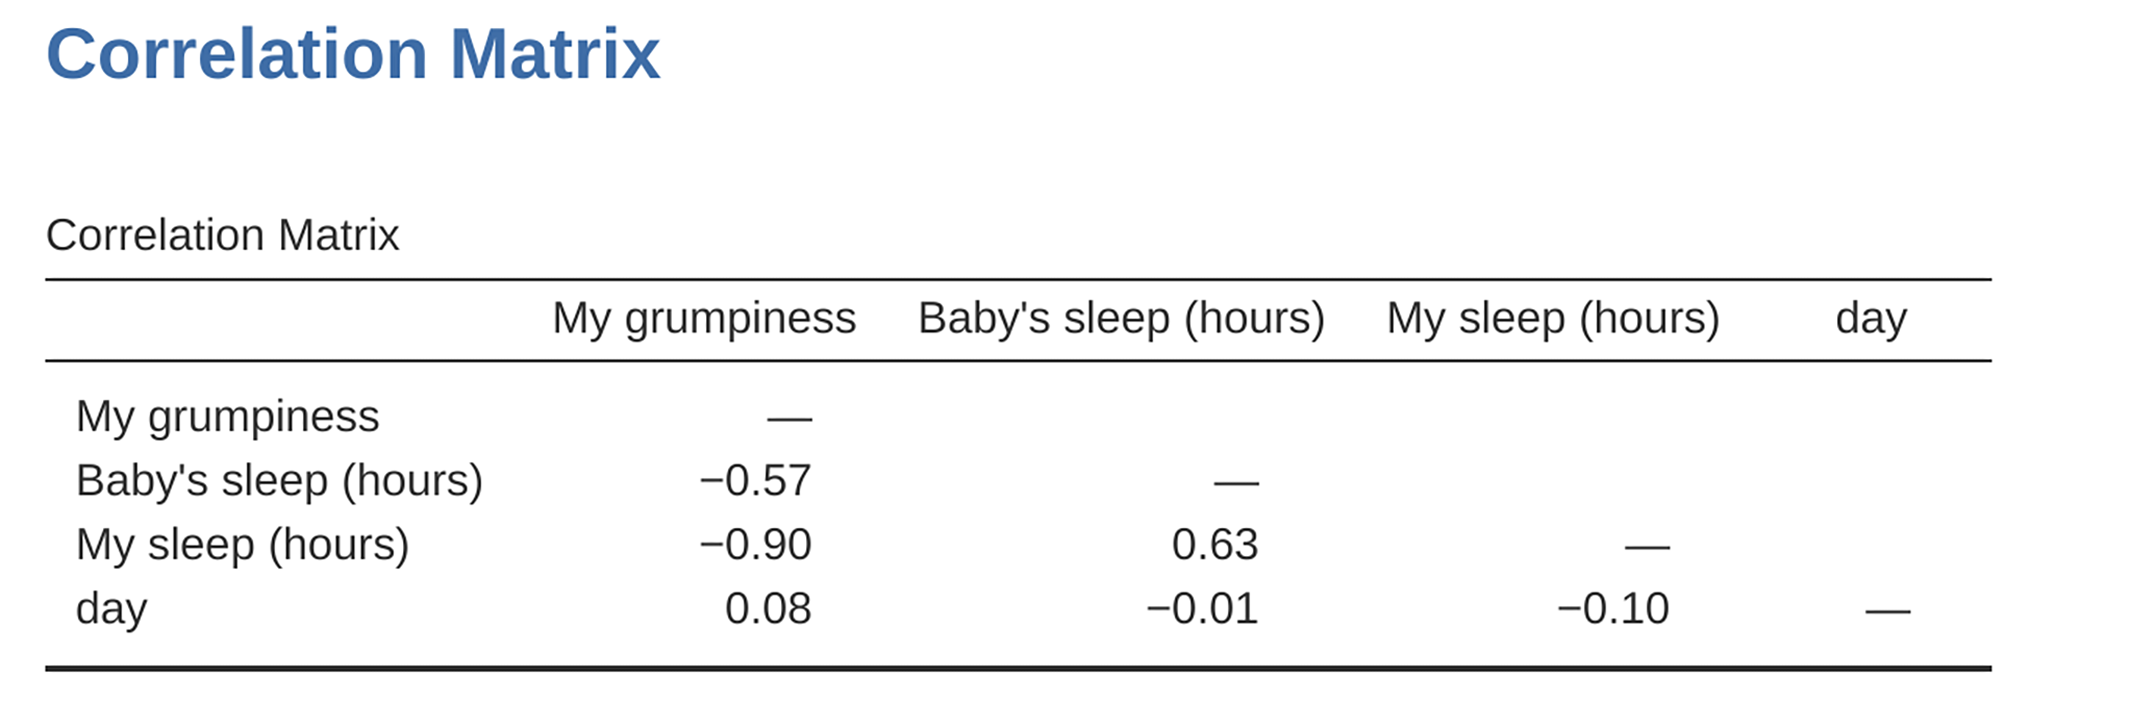
\includegraphics[width=1\textwidth,height=\textheight]{images/fig12-22.png} \hfill{}

\caption{\label{fig-fig12-22}Correlation matrix in jamovi for all four
variables}

\end{figure}

We have some fairly large correlations between some of our predictor
variables! When we run the regression model and look at the VIF values,
we see that the collinearity is causing a lot of uncertainty about the
coefficients. First, run the regression, as in Figure~\ref{fig-fig12-23}
and you can see from the VIF values that, yep, that's some mighty fine
collinearity there.

\begin{figure}

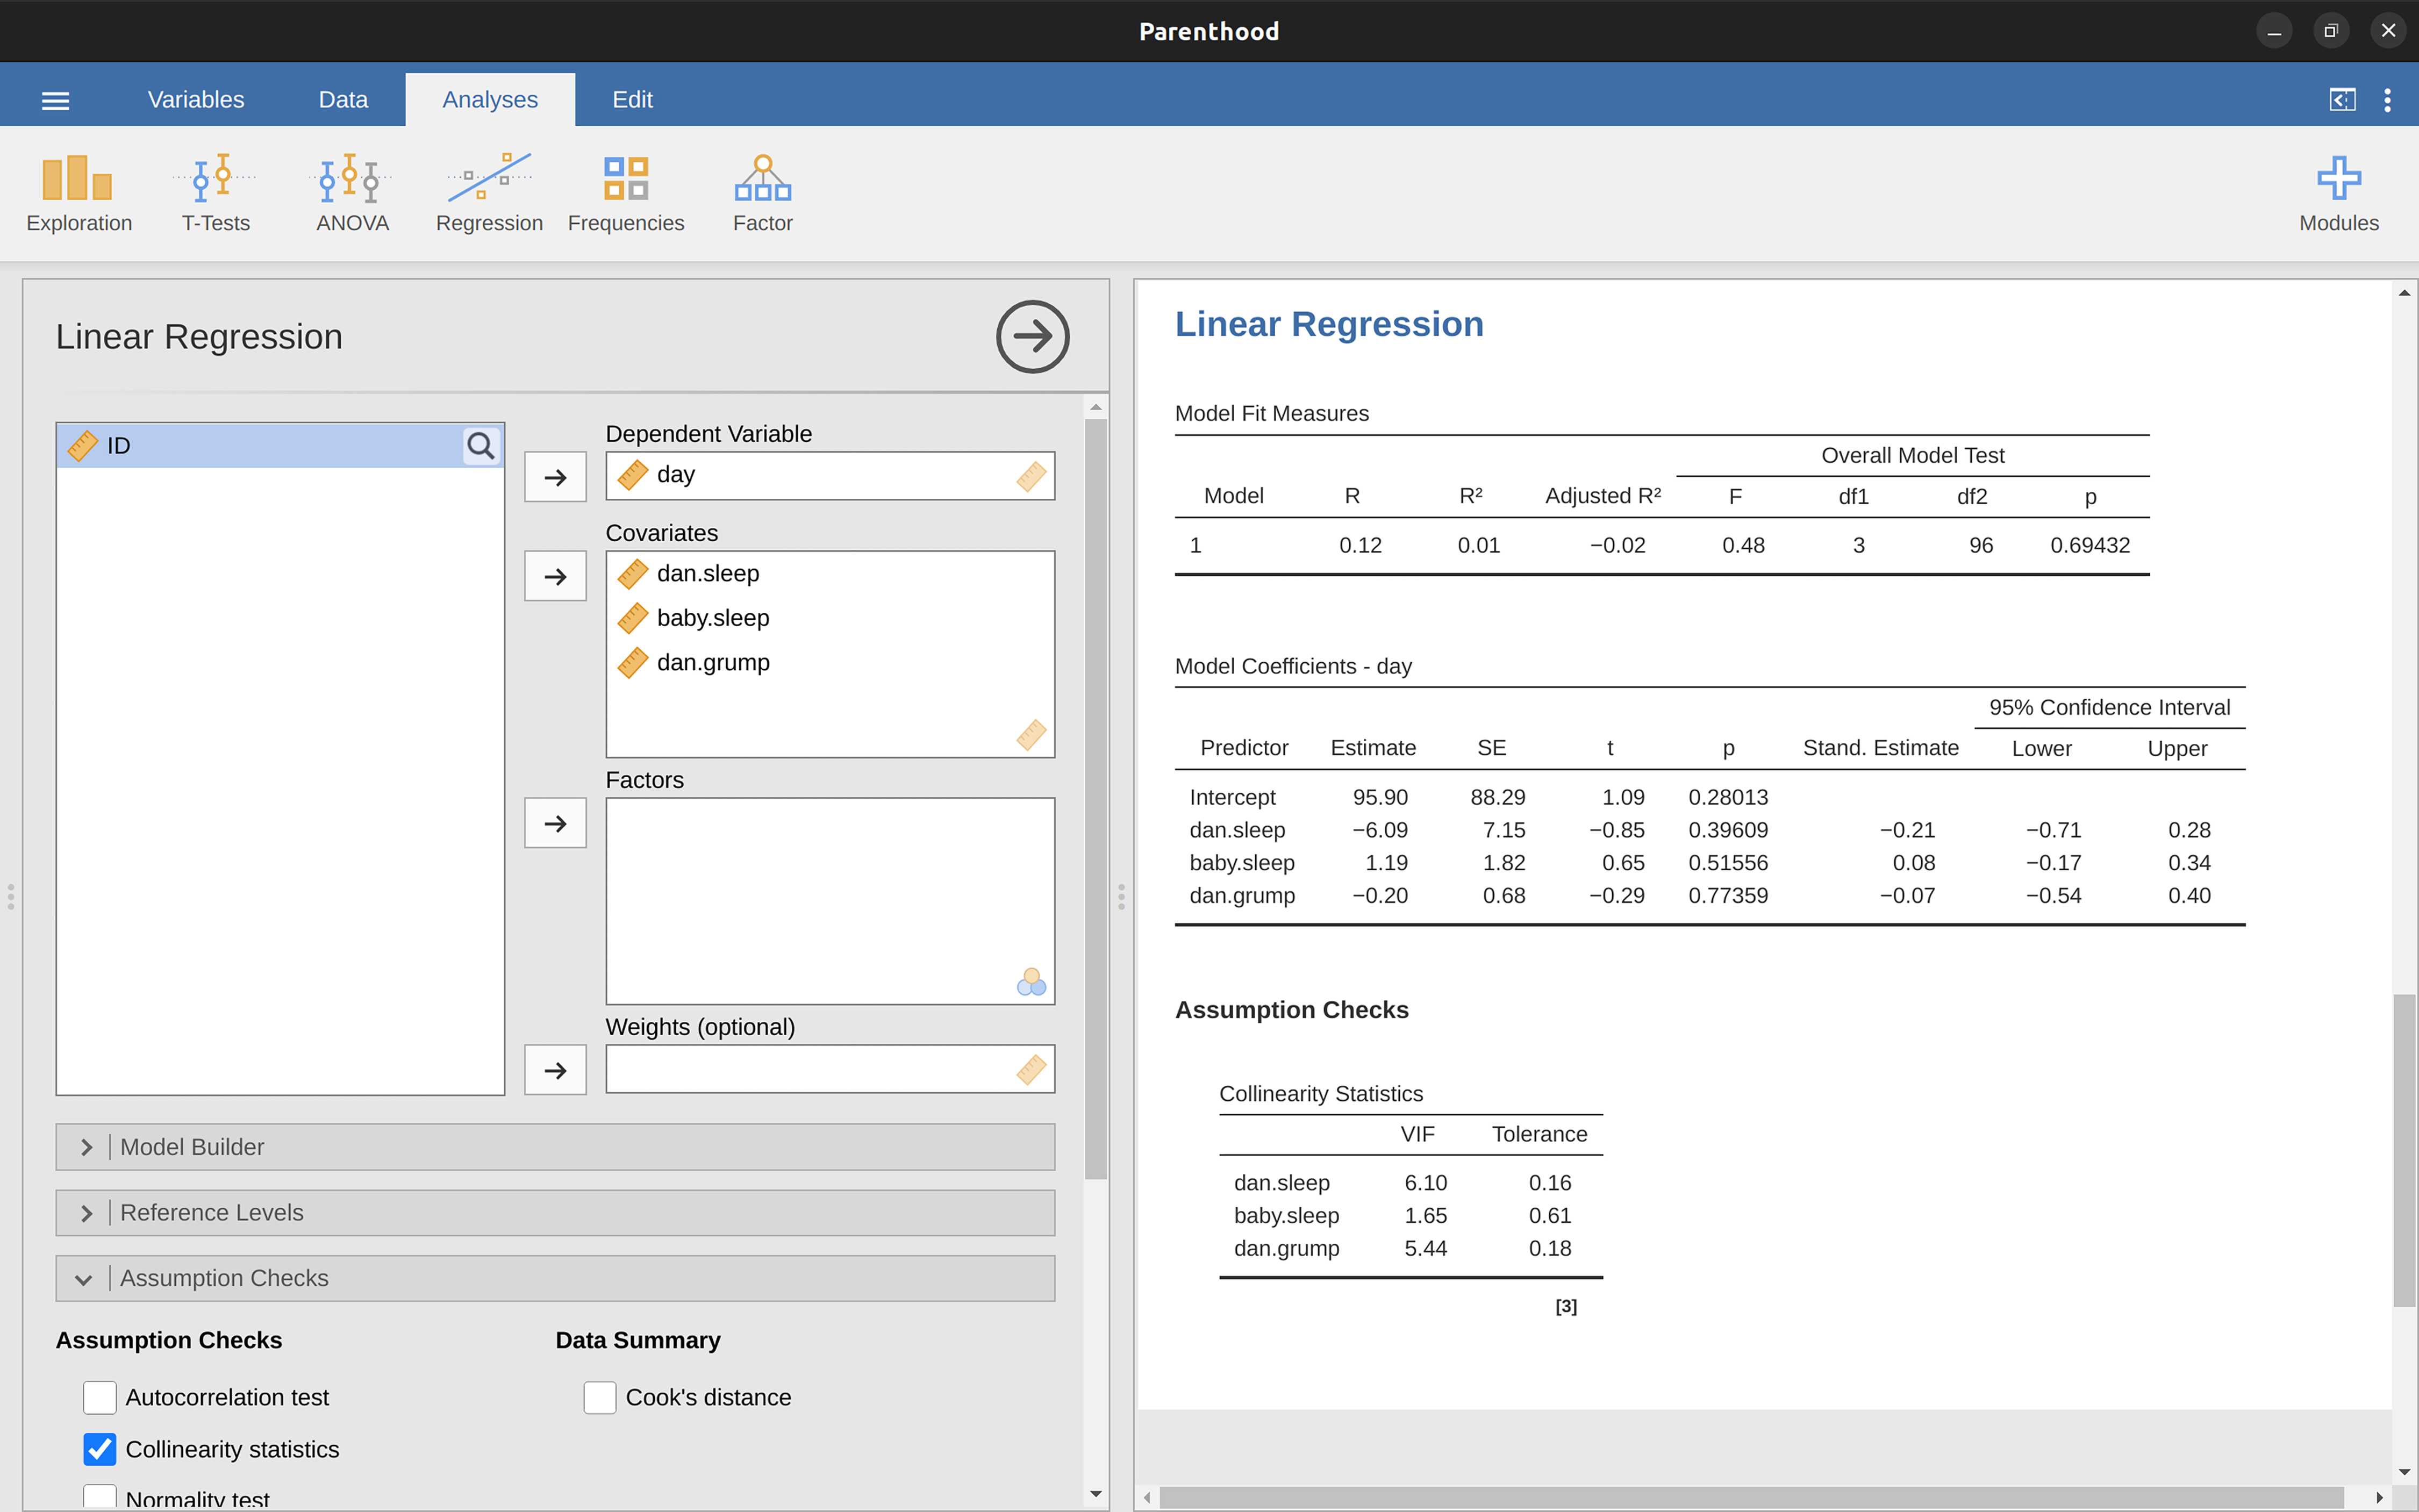
\includegraphics[width=1\textwidth,height=\textheight]{images/fig12-23.png} \hfill{}

\caption{\label{fig-fig12-23}Collinearity statistics for multiple
regression, produced in jamovi}

\end{figure}

\hypertarget{outliers-and-anomalous-data}{%
\subsection{Outliers and anomalous
data}\label{outliers-and-anomalous-data}}

One danger that you can run into with linear regression models is that
your analysis might be disproportionately sensitive to a smallish number
of ``unusual'' or ``anomalous'' observations. I discussed this idea
previously in \textbf{?@sec-Using-box-plots-to-detect-outliers} in the
context of discussing the outliers that get automatically identified by
the boxplot option under `Exploration' - `Descriptives', but this time
we need to be much more precise. In the context of linear regression,
there are three conceptually distinct ways in which an observation might
be called ``anomalous''. All three are interesting, but they have rather
different implications for your analysis.

The first kind of unusual observation is an \textbf{outlier}. The
definition of an outlier (in this context) is an observation that is
very different from what the regression model predicts. An example is
shown in Figure~\ref{fig-fig12-24}. In practice, we operationalise this
concept by saying that an outlier is an observation that has a very
large residual, \(\epsilon_i^*\). Outliers are interesting: a big
outlier might correspond to junk data, e.g., the variables might have
been recorded incorrectly in the data set, or some other defect may be
detectable. Note that you shouldn't throw an observation away just
because it's an outlier. But the fact that it's an outlier is often a
cue to look more closely at that case and try to find out why it's so
different.

\begin{figure}

\includegraphics[width=1\textwidth,height=\textheight]{12-Correlation-and-linear-regression_files/figure-pdf/fig-fig12-24-1.pdf} \hfill{}

\caption{\label{fig-fig12-24}An illustration of outliers. The solid line
shows the regression line with the anomalous outlier observation
included. The dashed line plots the regression line estimated without
the anomalous outlier observation included. The vertical line from the
outlier point to the dashed regression line illustrates the large
residual error for the outlier. The outlier has an unusual value on the
outcome (y-axis location) but not the predictor (x-axis location), and
lies a long way from the regression line}

\end{figure}

The second way in which an observation can be unusual is if it has high
\textbf{leverage}, which happens when the observation is very different
from all the other observations. This doesn't necessarily have to
correspond to a large residual. If the observation happens to be unusual
on all variables in precisely the same way, it can actually lie very
close to the regression line. An example of this is shown in
Figure~\ref{fig-fig12-24}. The leverage of an observation is
operationalised in terms of its hat value, usually written \(h_i\). The
formula for the hat value is rather complicated\footnote{Again, for the
  linear algebra fanatics: the ``hat matrix'' is defined to be that
  matrix \(H\) that converts the vector of observed values \(y\) into a
  vector of predicted values \(\hat{y}\), such that \(\hat{y} = Hy\).
  The name comes from the fact that this is the matrix that ``puts a hat
  on y''. The hat value of the i-th observation is the i-th diagonal
  element of this matrix (so technically I should be writing it as
  \(h_{ii}\) rather than \(h_i\)). And here's how it's calculated:
  \(H = X(X^{'}X)^{1}X^{'}\).} but its interpretation is not: \(h_i\) is
a measure of the extent to which the i-th observation is ``in control''
of where the regression line ends up going.

\begin{figure}

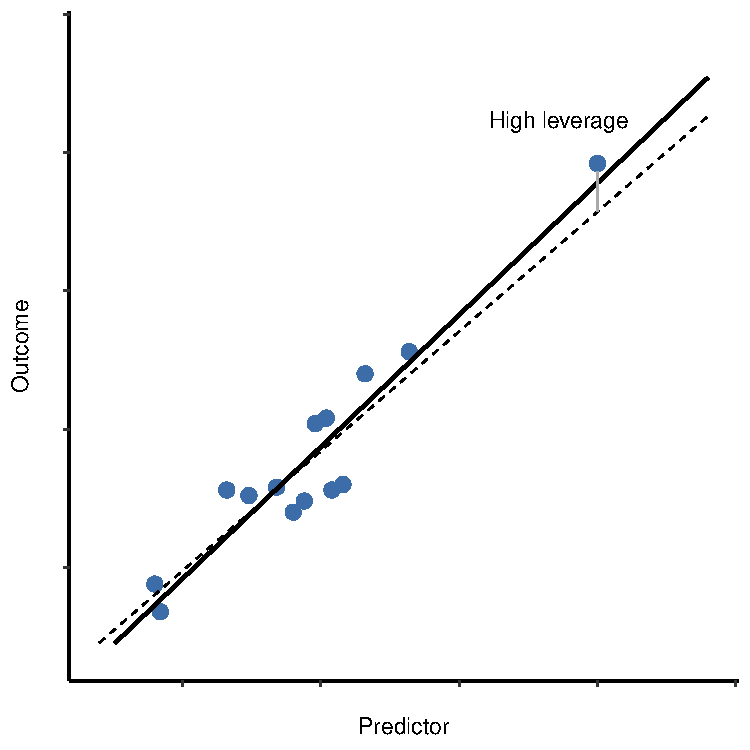
\includegraphics[width=1\textwidth,height=\textheight]{12-Correlation-and-linear-regression_files/figure-pdf/fig-fig12-25-1.pdf} \hfill{}

\caption{\label{fig-fig12-25}An illustration of high leverage points.
The anomalous observation in this case is unusual both in terms of the
predictor (x-axis) and the outcome (y-axis), but this unusualness is
highly consistent with the pattern of correlations that exists among the
other observations. The observation falls very close to the regression
line and does not distort it by very much}

\end{figure}

In general, if an observation lies far away from the other ones in terms
of the predictor variables, it will have a large hat value (as a rough
guide, high leverage is when the hat value is more than 2-3 times the
average; and note that the sum of the hat values is constrained to be
equal to \(K + 1\)). High leverage points are also worth looking at in
more detail, but they're much less likely to be a cause for concern
unless they are also outliers.

This brings us to our third measure of unusualness, the
\textbf{influence} of an observation. A high influence observation is an
outlier that has high leverage. That is, it is an observation that is
very different to all the other ones in some respect, and also lies a
long way from the regression line. This is illustrated in
Figure~\ref{fig-fig12-26}. Notice the contrast to the previous two
figures. Outliers don't move the regression line much and neither do
high leverage points. But something that is both an outlier and has high
leverage, well that has a big effect on the regression line. That's why
we call these points high influence, and it's why they're the biggest
worry. We operationalise influence in terms of a measure known as
\textbf{Cook's distance}.\footnote{\(D_i=\frac{{\epsilon_i^*}^2}{K+1} \times \frac{h_i}{1-h_i}\)
  Notice that this is a multiplication of something that measures the
  outlier-ness of the observation (the bit on the left), and something
  that measures the leverage of the observation (the bit on the right).}

\begin{figure}

\includegraphics[width=1\textwidth,height=\textheight]{12-Correlation-and-linear-regression_files/figure-pdf/fig-fig12-26-1.pdf} \hfill{}

\caption{\label{fig-fig12-26}An illustration of high influence points.
In this case, the anomalous observation is highly unusual on the
predictor variable (x-axis), and falls a long way from the regression
line. As a consequence, the regression line is highly distorted, even
though (in this case) the anomalous observation is entirely typical in
terms of the outcome variable (y-axis)}

\end{figure}

In order to have a large Cook's distance an observation must be a fairly
substantial outlier and have high leverage. As a rough guide, Cook's
distance greater than 1 is often considered large (that's what I
typically use as a quick and dirty rule).

In jamovi, information about Cook's distance can be calculated by
clicking on the `Cook's Distance' checkbox in the `Assumption Checks' -
`Data Summary' options. When you do this, for the multiple regression
model we have been using as an example in this chapter, you get the
results as shown in Figure~\ref{fig-fig12-27}.

\begin{figure}

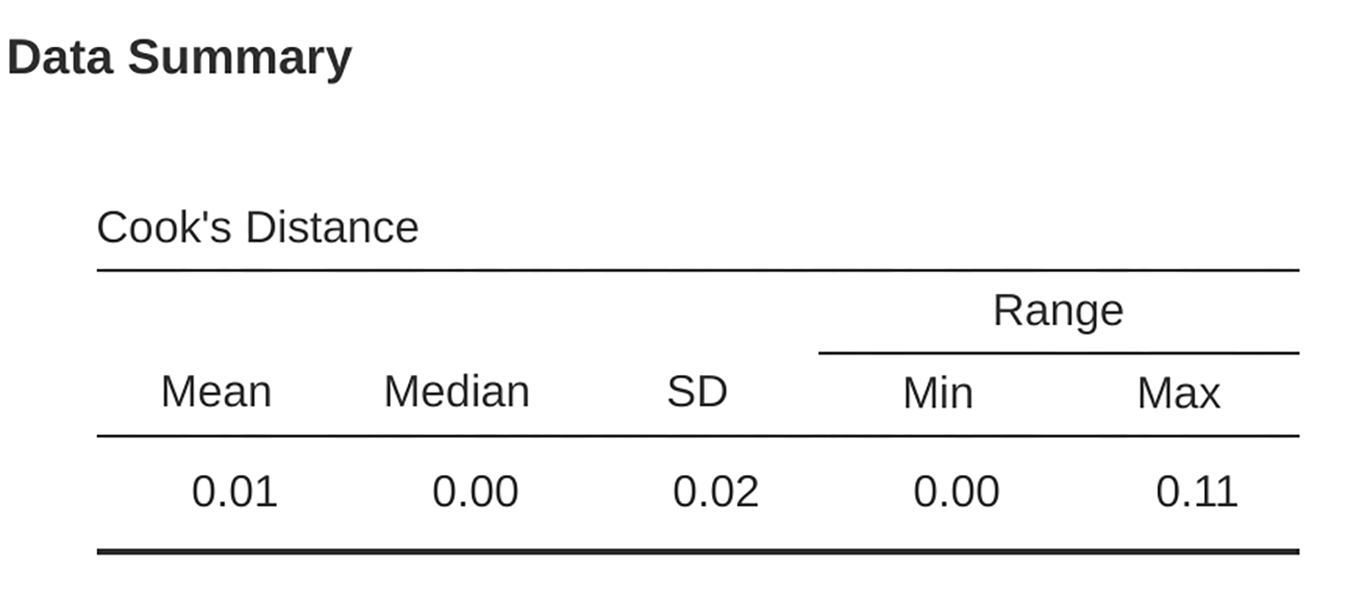
\includegraphics[width=1\textwidth,height=\textheight]{images/fig12-27.png} \hfill{}

\caption{\label{fig-fig12-27}jamovi output showing the table for the
Cooks distance statistics}

\end{figure}

You can see that, in this example, the mean Cook's distance value is
\(0.01\), and the range is from \(0.00\) to \(0.11\), so this is some
way off the rule of thumb figure mentioned above that a Cook's distance
greater than 1 is considered large.

An obvious question to ask next is, if you do have large values of
Cook's distance what should you do? As always, there's no hard and fast
rule. Probably the first thing to do is to try running the regression
with the outlier with the greatest Cook's distance\footnote{In jamovi
  you can save the Cook's distance values to the dataset, then draw a
  boxplot of the Cook's distance values to identify the specific
  outliers. Or you could use a more powerful regression program such as
  the ``car'' package in R which has more options for advanced
  regression diagnostic analysis.} excluded and see what happens to the
model performance and to the regression coefficients. If they really are
substantially different, it's time to start digging into your data set
and your notes that you no doubt were scribbling as your ran your study.
Try to figure out why the point is so different. If you start to become
convinced that this one data point is badly distorting your results then
you might consider excluding it, but that's less than ideal unless you
have a solid explanation for why this particular case is qualitatively
different from the others and therefore deserves to be handled
separately.

\hypertarget{model-selection}{%
\section{Model selection}\label{model-selection}}

One fairly major problem that remains is the problem of ``model
selection''. That is, if we have a data set that contains several
variables, which ones should we include as predictors, and which ones
should we not include? In other words, we have a problem of
\textbf{variable selection}. In general, model selection is a complex
business but it's made somewhat simpler if we restrict ourselves to the
problem of choosing a subset of the variables that ought to be included
in the model. Nevertheless, I'm not going to try covering even this
reduced topic in a lot of detail. Instead, I'll talk about two broad
principles that you need to think about, and then discuss one concrete
tool that jamovi provides to help you select a subset of variables to
include in your model. First, the two principles:

\begin{itemize}
\item
  It's nice to have an actual substantive basis for your choices. That
  is, in a lot of situations you the researcher have good reasons to
  pick out a smallish number of possible regression models that are of
  theoretical interest. These models will have a sensible interpretation
  in the context of your field. Never discount the importance of this.
  Statistics serves the scientific process, not the other way around.
\item
  To the extent that your choices rely on statistical inference, there
  is a trade off between simplicity and goodness of fit. As you add more
  predictors to the model you make it more complex. Each predictor adds
  a new free parameter (i.e., a new regression coefficient), and each
  new parameter increases the model's capacity to ``absorb'' random
  variations. So the goodness of fit (e.g., \(R^2\)) continues to rise,
  sometimes trivially or by chance, as you add more predictors no matter
  what. If you want your model to be able to generalise well to new
  observations you need to avoid throwing in too many variables.
\end{itemize}

This latter principle is often referred to as \textbf{Ockham's razor}
and is often summarised in terms of the following pithy saying: do not
multiply entities beyond necessity. In this context, it means don't
chuck in a bunch of largely irrelevant predictors just to boost your
\(R^2\). Hmm. Yeah, the original was better.

In any case, what we need is an actual mathematical criterion that will
implement the qualitative principle behind Ockham's razor in the context
of selecting a regression model. As it turns out there are several
possibilities. The one that I'll talk about is the \textbf{Akaike
information criterion} (AIC) (Akaike, 1974) simply because it's
available as an option in jamovi. \footnote{In the context of a linear
  regression model (and ignoring terms that don't depend on the model in
  any way!), the AIC for a model that has \(K\) predictor variables plus
  an intercept is \(AIC=\frac{SS_{res}}{\hat{\sigma}^2}+2K\).}

The smaller the AIC value, the better the model performance. If we
ignore the low level details it's fairly obvious what the AIC does. On
the left we have a term that increases as the model predictions get
worse; on the right we have a term that increases as the model
complexity increases. The best model is the one that fits the data well
(low residuals, left-hand side) using as few predictors as possible (low
K, right-hand side). In short, this is a simple implementation of
Ockham's razor.

AIC can be added to the `Model Fit Measures' output Table when the `AIC'
checkbox is clicked, and a rather clunky way of assessing different
models is seeing if the AIC value is lower if you remove one or more of
the predictors in the regression model. This is the only way currently
implemented in jamovi, but there are alternatives in other more powerful
programmes, such as R. These alternative methods can automate the
process of selectively removing (or adding) predictor variables to find
the best AIC. Although these methods are not implemented in jamovi, I
will mention them briefly below just so you know about them.

\hypertarget{backward-elimination}{%
\subsection{Backward elimination}\label{backward-elimination}}

In backward elimination you start with the complete regression model,
including all possible predictors. Then, at each ``step'' we try all
possible ways of removing one of the variables, and whichever of these
is best (in terms of lowest AIC value) is accepted. This becomes our new
regression model, and we then try all possible deletions from the new
model, again choosing the option with lowest AIC. This process continues
until we end up with a model that has a lower AIC value than any of the
other possible models that you could produce by deleting one of its
predictors.

\hypertarget{forward-selection}{%
\subsection{Forward selection}\label{forward-selection}}

As an alternative, you can also try \textbf{forward selection}. This
time around we start with the smallest possible model as our start
point, and only consider the possible additions to the model. However,
there's one complication. You also need to specify what the largest
possible model you're willing to entertain is.

Although backward and forward selection can lead to the same conclusion,
they don't always.

\hypertarget{a-caveat}{%
\subsection{A caveat}\label{a-caveat}}

Automated variable selection methods are seductive things, especially
when they're bundled up in (fairly) simple functions in powerful
statistical programmes. They provide an element of objectivity to your
model selection, and that's kind of nice. Unfortunately, they're
sometimes used as an excuse for thoughtlessness. No longer do you have
to think carefully about which predictors to add to the model and what
the theoretical basis for their inclusion might be. Everything is solved
by the magic of AIC. And if we start throwing around phrases like
Ockham's razor, well it sounds like everything is wrapped up in a nice
neat little package that no-one can argue with.

Or, perhaps not. Firstly, there's very little agreement on what counts
as an appropriate model selection criterion. When I was taught backward
elimination as an undergraduate, we used F-tests to do it, because that
was the default method used by the software. I've described using AIC,
and since this is an introductory text that's the only method I've
described, but the AIC is hardly the Word of the Gods of Statistics.
It's an approximation, derived under certain assumptions, and it's
guaranteed to work only for large samples when those assumptions are
met. Alter those assumptions and you get a different criterion, like the
Bayesian Information Criterion (BIC) for instance (also available in
jamovi). Take a different approach again and you get the normalised
maximum likelihood (NML) criterion. Decide that you're a Bayesian and
you get model selection based on posterior odds ratios. Then there are a
bunch of regression specific tools that I haven't mentioned. And so on.
All of these different methods have strengths and weaknesses, and some
are easier to calculate than others (AIC is probably the easiest of the
lot, which might account for its popularity). Almost all of them produce
the same answers when the answer is ``obvious'' but there's a fair
amount of disagreement when the model selection problem becomes hard.

What does this mean in practice? Well, you could go and spend several
years teaching yourself the theory of model selection, learning all the
ins and outs of it so that you could finally decide on what you
personally think the right thing to do is. Speaking as someone who
actually did that, I wouldn't recommend it. You'll probably come out the
other side even more confused than when you started. A better strategy
is to show a bit of common sense. If you're staring at the results of an
automated backwards or forwards selection procedure, and the model that
makes sense is close to having the smallest AIC but is narrowly defeated
by a model that doesn't make any sense, then trust your instincts.
Statistical model selection is an inexact tool, and as I said at the
beginning, interpretability matters.

\hypertarget{comparing-two-regression-models}{%
\subsection{Comparing two regression
models}\label{comparing-two-regression-models}}

An alternative to using automated model selection procedures is for the
researcher to explicitly select two or more regression models to compare
to each other. You can do this in a few different ways, depending on
what research question you're trying to answer. Suppose we want to know
whether or not the amount of sleep that my son got has any relationship
to my grumpiness, over and above what we might expect from the amount of
sleep that I got. We also want to make sure that the day on which we
took the measurement has no influence on the relationship. That is,
we're interested in the relationship between baby.sleep and dani.grump,
and from that perspective dani.sleep and day are nuisance variable or
\textbf{covariates} that we want to control for. In this situation, what
we would like to know is whether dani.grump \textasciitilde{} dani.sleep
+ day + baby .sleep (which I'll call Model 2, or M2) is a better
regression model for these data than dani.grump \textasciitilde{}
dani.sleep + day (which I'll call Model 1, or M1). There are two
different ways we can compare these two models, one based on a model
selection criterion like AIC, and the other based on an explicit
hypothesis test. I'll show you the AIC based approach first because it's
simpler, and follows naturally from discussion in the last section. The
first thing I need to do is actually run the two regressions, note the
AIC for each one, and then select the model with the smaller AIC value
as it is judged to be the better model for these data. Actually, don't
do this just yet. Read on because there is an easy way in jamovi to get
the AIC values for different models included in one table.\footnote{While
  I'm on this topic I should point out that the empirical evidence
  suggests that BIC is a better criterion than AIC. In most simulation
  studies that I've seen, BIC does a much better job of selecting the
  correct model.}

A somewhat different approach to the problem comes out of the hypothesis
testing framework. Suppose you have two regression models, where one of
them (Model 1) contains a subset of the predictors from the other one
(Model 2). That is, Model 2 contains all of the predictors included in
Model 1, plus one or more additional predictors. When this happens we
say that Model 1 is nested within Model 2, or possibly that Model 1 is a
submodel of Model 2. Regardless of the terminology, what this means is
that we can think of Model 1 as a null hypothesis and Model 2 as an
alternative hypothesis. And in fact we can construct an \emph{F}-test
for this in a fairly straightforward fashion.\footnote{We can fit both
  models to the data and obtain a residual sum of squares for both
  models. I'll denote these as \(SS_{res}^{(1)}\) and \(SS_{res}^{(2)}\)
  respectively. The superscripting here just indicates which model we're
  talking about. Then our \emph{F} statistic is
  \[F= \frac {\frac {SS _{res}^{(1)} - SS_{res}^{(2)}} {k}}   {\frac{SS_{res}^2} {N-p-1} }\]
  where \(N\) is the number of observations, \(p\) is the number of
  predictors in the full model (not including the intercept), and \(k\)
  is the difference in the number of parameters between the two
  models.\(^d\) The degrees of freedom here are \(k\) and \(N -p-1\).
  Note that it's often more convenient to think about the difference
  between those two \(SS\) values as a sum of squares in its own right.
  That is \[SS_\Delta=SS_{res}^{(1)}-SS_{res}^{(2)}\] The reason why
  this is helpful is that we can express \(SS_\Delta\) as a measure of
  the extent to which the two models make different predictions about
  the the outcome variable. Specifically,
  \[SS_\Delta=\sum_i{(\hat{y}_i^{(2)}-\hat{y}_i^{(1)})^2}\] where
  \(\hat{y}_{i^{(1)}}\) is the predicted value for \(y_i\) according to
  model \(M_1\) and \(\hat{y}_{i^{(2)}}\) is the predicted value for
  \(y_i\) according to model \(M_2\). --- \(^d\) It's worth noting in
  passing that this same \emph{F} statistic can be used to test a much
  broader range of hypotheses than those that I'm mentioning here. Very
  briefly, notice that the nested model \(M_1\) corresponds to the full
  model \(M_2\) when we constrain some of the regression coefficients to
  zero. It is sometimes useful to construct sub-models by placing other
  kinds of constraints on the regression coefficients. For instance,
  maybe two different coefficients might have to sum to zero. You can
  construct hypothesis tests for those kind of constraints too, but it
  is somewhat more complicated and the sampling distribution for \(F\)
  can end up being something known as the non-central \emph{F}
  distribution, which is way beyond the scope of this book! All I want
  to do is alert you to this possibility.}

Okay, so that's the hypothesis test that we use to compare two
regression models to one another. Now, how do we do it in jamovi? The
answer is to use the `Model Builder' option and specify the Model 1
predictors dani.sleep and day in `Block 1' and then add the additional
predictor from Model 2 (baby.sleep) in `Block 2', as in
Figure~\ref{fig-fig12-27}. This shows, in the `Model Comparisons' Table,
that for the comparisons between Model 1 and Model 2,
\(F(1,96) = 0.00\), \(p = 0.954\). Since we have p \textgreater{} .05 we
retain the null hypothesis (M1). This approach to regression, in which
we add all of our covariates into a null model, then add the variables
of interest into an alternative model, and then compare the two models
in a hypothesis testing framework, is often referred to as
\textbf{hierarchical regression}.

We can also use this `Model Comparison' option to display a table that
shows the AIC and BIC for each model, making it easy to compare and
identify which model has the lowest value, as in
Figure~\ref{fig-fig12-28}.

\begin{figure}

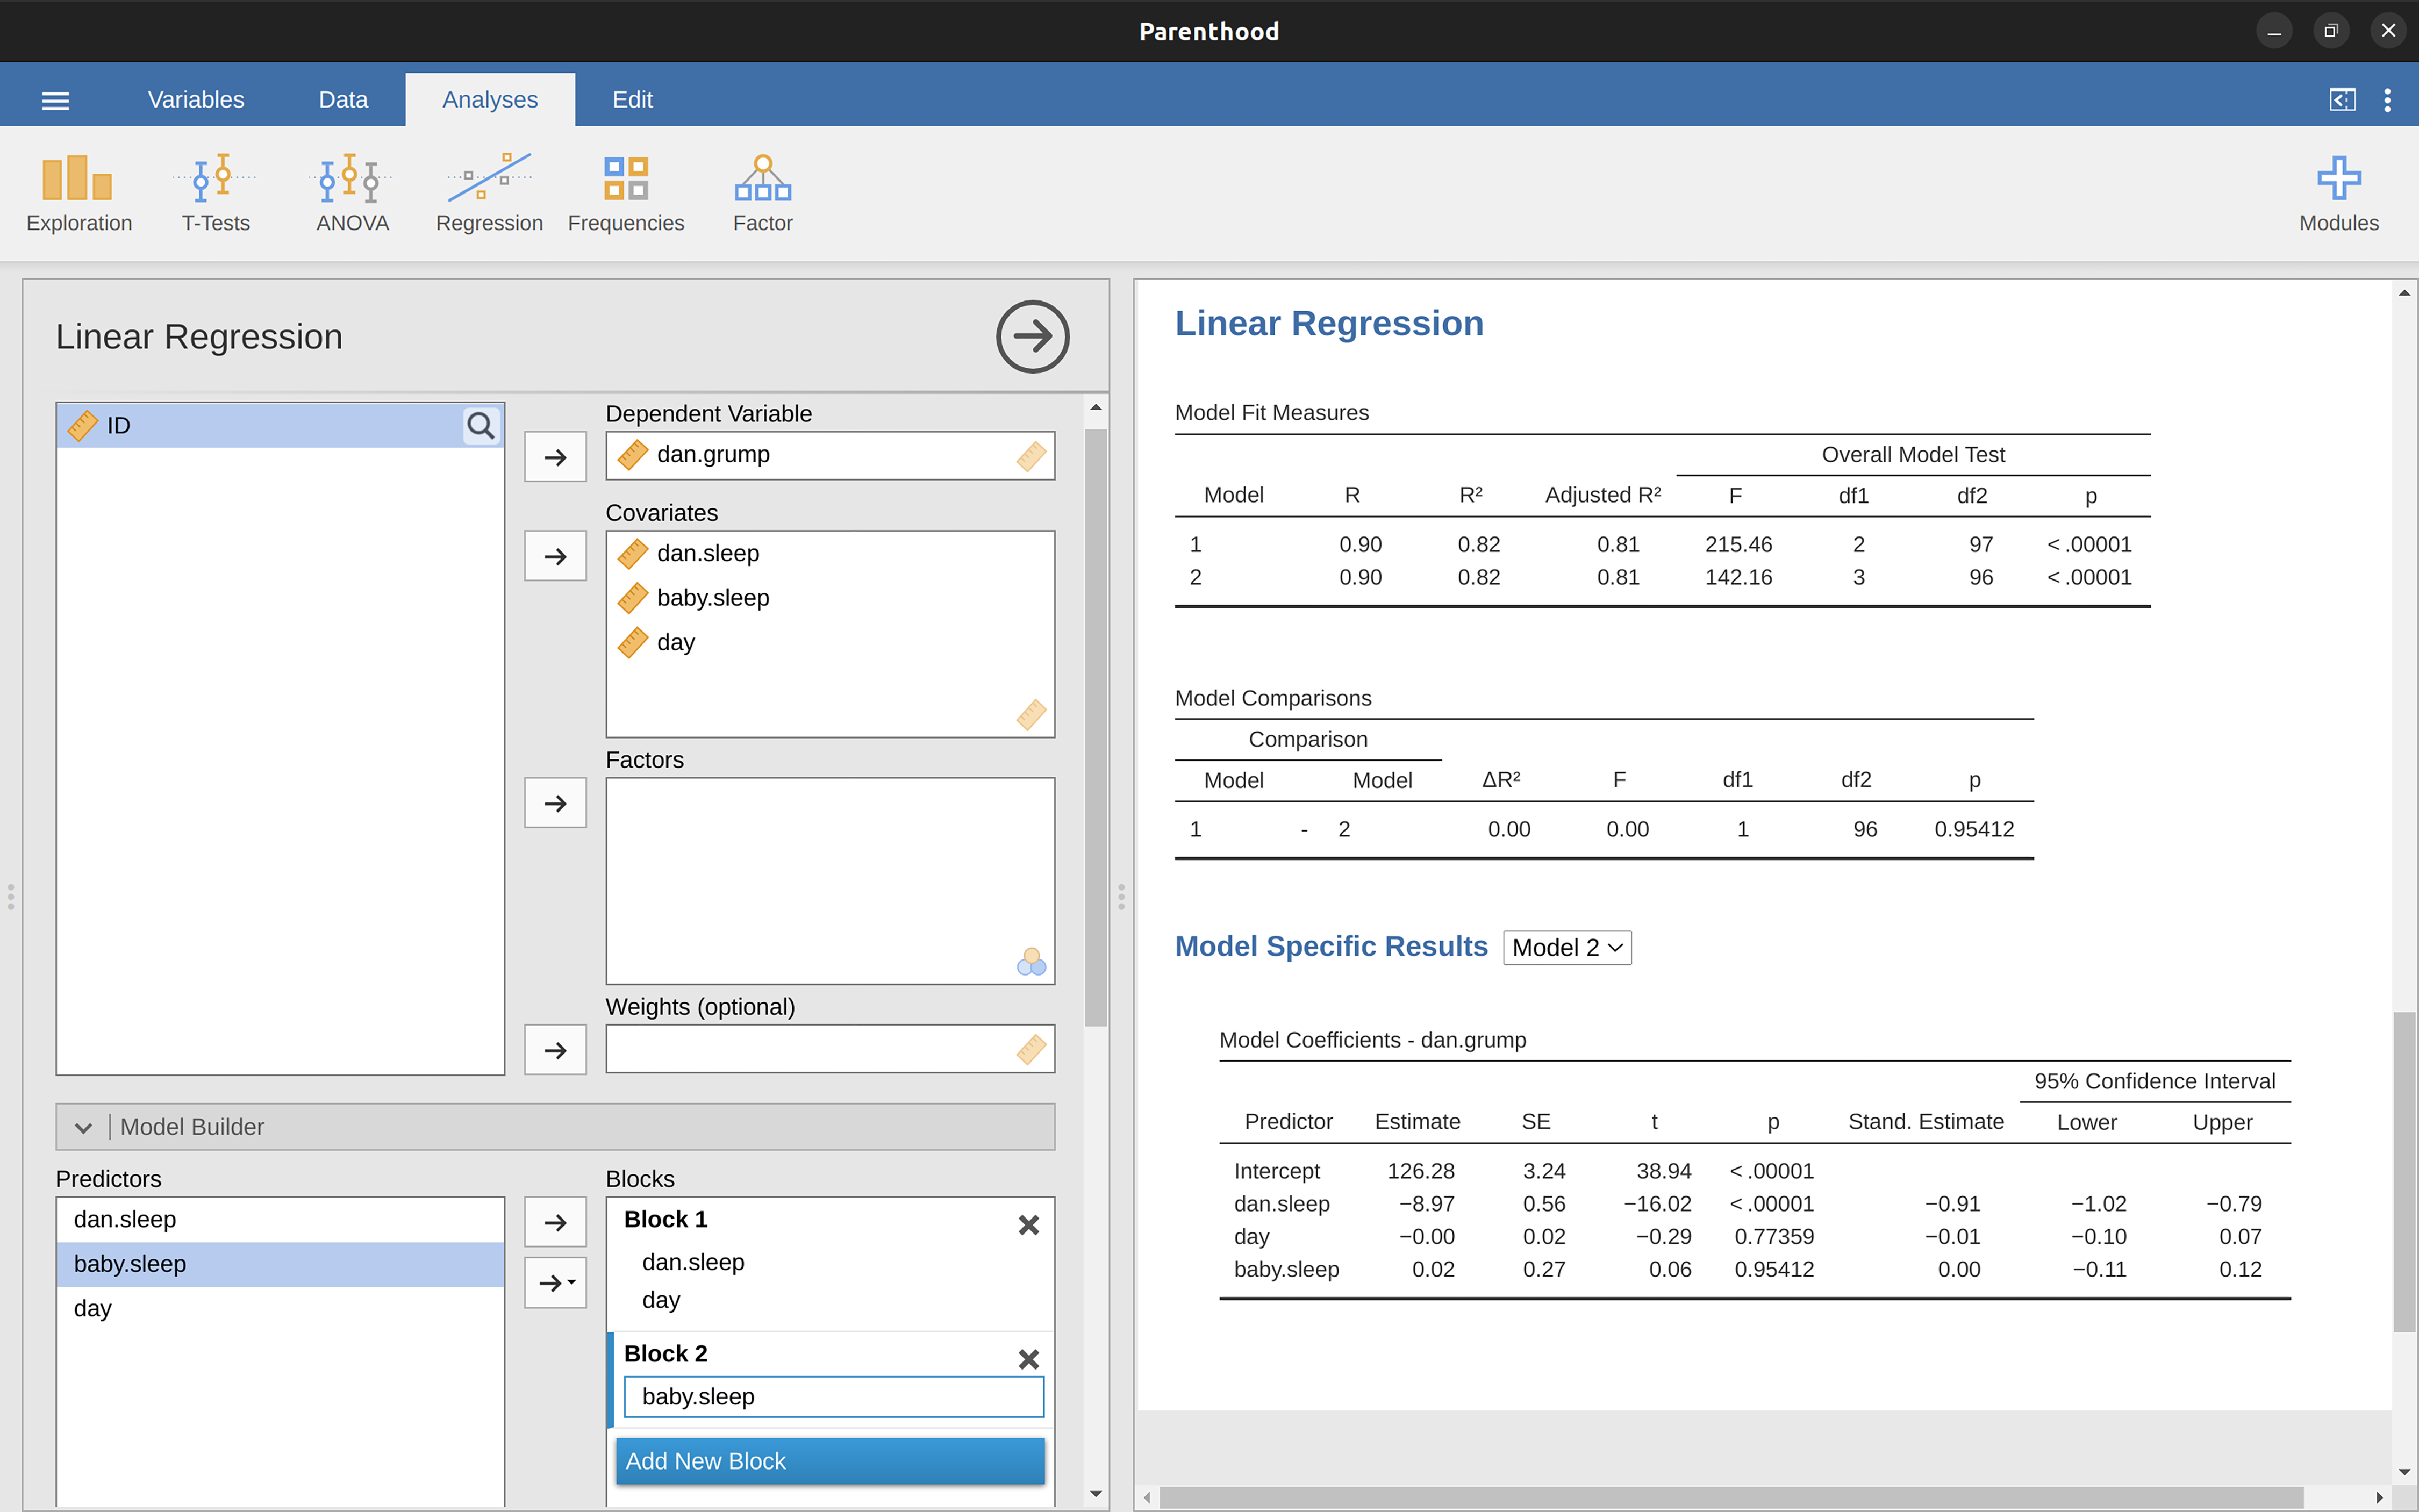
\includegraphics[width=1\textwidth,height=\textheight]{images/fig12-28.png} \hfill{}

\caption{\label{fig-fig12-28}Model comparison in jamovi using the `Model
Builder' option}

\end{figure}

\hypertarget{summary}{%
\section{Summary}\label{summary}}

\begin{itemize}
\tightlist
\item
  Want to know how strong the relationship is between two variables?
  Calculate \protect\hyperlink{correlations}{Correlations}.
\item
  Drawing \protect\hyperlink{scatterplots}{Scatterplots}.
\item
  Basic ideas about
  \protect\hyperlink{what-is-a-linear-regression-model}{What is a linear
  regression model?} and
  \protect\hyperlink{estimating-a-linear-regression-model}{Estimating a
  linear regression model}.
\item
  \protect\hyperlink{multiple-linear-regression}{Multiple linear
  regression}.
\item
  \protect\hyperlink{quantifying-the-fit-of-the-regression-model}{Quantifying
  the fit of the regression model} using \(R^2\).
\item
  \protect\hyperlink{hypothesis-tests-for-regression-models}{Hypothesis
  tests for regression models}.
\item
  In \protect\hyperlink{regarding-regression-coefficients}{Regarding
  regression coefficients} we talked about calculating
  \protect\hyperlink{confidence-intervals-for-the-coefficients}{Confidence
  intervals for the coefficients} and
  \protect\hyperlink{calculating-standardised-regression-coefficients}{Calculating
  standardised regression coefficients}.
\item
  The \protect\hyperlink{assumptions-of-regression}{Assumptions of
  regression} and \protect\hyperlink{sec-Model-checking}{Model
  checking}.
\item
  Regression \protect\hyperlink{model-selection}{Model selection}.
\end{itemize}

\bookmarksetup{startatroot}

\hypertarget{sec-Comparing-several-means-one-way-ANOVA}{%
\chapter{Comparing several means (one-way
ANOVA)}\label{sec-Comparing-several-means-one-way-ANOVA}}

This chapter introduces one of the most widely used tools in
psychological statistics, known as ``the analysis of variance'', but
usually referred to as ANOVA. The basic technique was developed by Sir
Ronald Fisher in the early 20th century and it is to him that we owe the
rather unfortunate terminology. The term ANOVA is a little misleading,
in two respects. Firstly, although the name of the technique refers to
variances, ANOVA is concerned with investigating differences in means.
Secondly, there are several different things out there that are all
referred to as ANOVAs, some of which have only a very tenuous connection
to one another. Later on in the book we'll encounter a range of
different ANOVA methods that apply in quite different situations, but
for the purposes of this chapter we'll only consider the simplest form
of ANOVA, in which we have several different groups of observations, and
we're interested in finding out whether those groups differ in terms of
some outcome variable of interest. This is the question that is
addressed by a one-way ANOVA.

The structure of this chapter is as follows: first I'll introduce a
fictitious data set that we'll use as a running example throughout the
chapter. After introducing the data, I'll describe the mechanics of how
a one-way ANOVA actually works
\protect\hyperlink{sec-How-ANOVA-works}{How ANOVA works} and then focus
on how you can run one in jamovi
\protect\hyperlink{running-an-anova-in-jamovi}{Running an ANOVA in
jamovi}. These two sections are the core of the chapter.

The remainder of the chapter discusses a range of important topics that
inevitably arise when running an ANOVA, namely how to calculate effect
sizes, post hoc tests and corrections for multiple comparisons and the
assumptions that ANOVA relies upon. We'll also talk about how to check
those assumptions and some of the things you can do if the assumptions
are violated. Then we'll cover repeated measures ANOVA.

\hypertarget{an-illustrative-data-set}{%
\section{An illustrative data set}\label{an-illustrative-data-set}}

Suppose you've become involved in a clinical trial in which you are
testing a new antidepressant drug called \emph{Joyzepam}. In order to
construct a fair test of the drug's effectiveness, the study involves
three separate drugs to be administered. One is a placebo, and the other
is an existing antidepressant / anti-anxiety drug called
\emph{Anxifree}. A collection of 18 participants with moderate to severe
depression are recruited for your initial testing. Because the drugs are
sometimes administered in conjunction with psychological therapy, your
study includes 9 people undergoing cognitive behavioural therapy (CBT)
and 9 who are not. Participants are randomly assigned (doubly blinded,
of course) a treatment, such that there are 3 CBT people and 3
no-therapy people assigned to each of the 3 drugs. A psychologist
assesses the mood of each person after a 3-month run with each drug, and
the overall improvement in each person's mood is assessed on a scale
ranging from \(-5\) to \(+5\). With that as the study design, let's now
load up the data file in \emph{clinicaltrial.csv} . We can see that this
data set contains the three variables drug, therapy and mood.gain.

For the purposes of this chapter, what we're really interested in is the
effect of drug on mood.gain. The first thing to do is calculate some
descriptive statistics and draw some graphs. In the
\textbf{?@sec-Descriptive-statistics} chapter we showed you how to do
this, and some of the descriptive statistics we can calculate in jamovi
are shown in Figure~\ref{fig-fig13-1}.

\begin{figure}

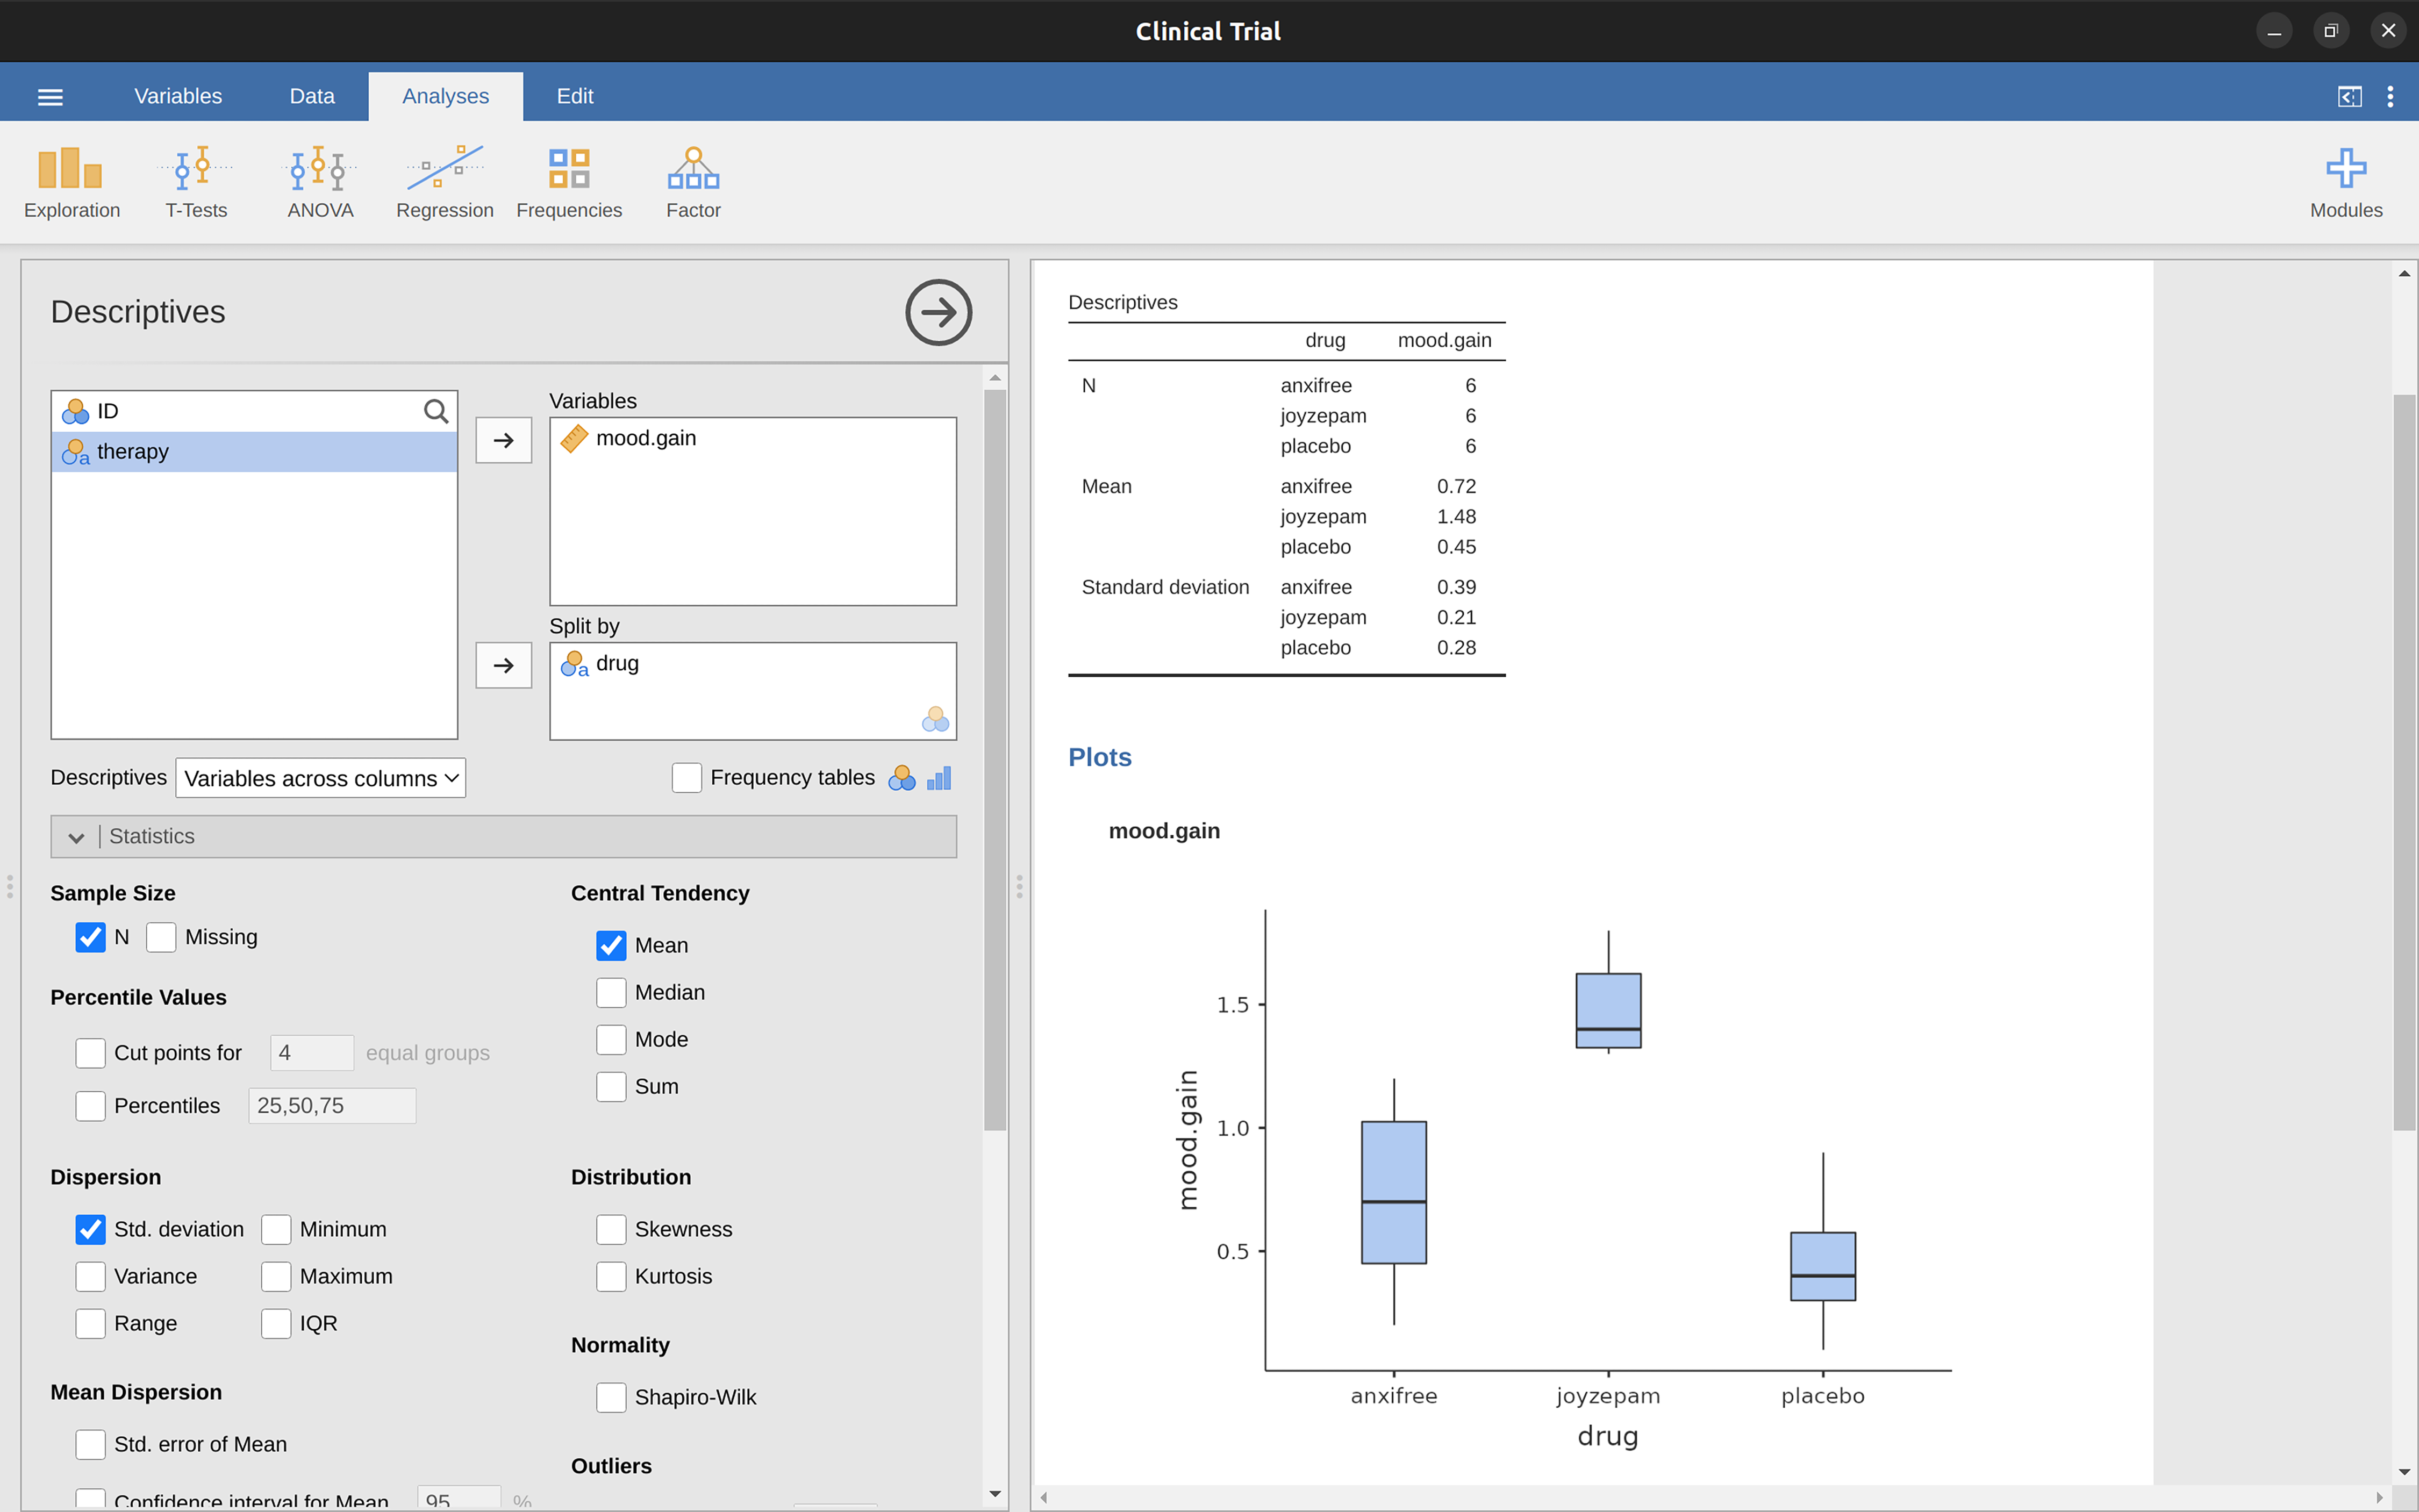
\includegraphics[width=1\textwidth,height=\textheight]{images/fig13-1.png} \hfill{}

\caption{\label{fig-fig13-1}Descriptives for mood gain, and box plots by
drug administered}

\end{figure}

As the plot makes clear, there is a larger improvement in mood for
participants in the Joyzepam group than for either the Anxifree group or
the placebo group. The Anxifree group shows a larger mood gain than the
control group, but the difference isn't as large. The question that we
want to answer is are these difference ``real'', or are they just due to
chance?

\hypertarget{sec-How-ANOVA-works}{%
\section{How ANOVA works}\label{sec-How-ANOVA-works}}

In order to answer the question posed by our clinical trial data we're
going to run a one-way ANOVA. I'm going to start by showing you how to
do it the hard way, building the statistical tool from the ground up and
showing you how you could do it if you didn't have access to any of the
cool built-in ANOVA functions in jamovi. And I hope you'll read it
carefully, try to do it the long way once or twice to make sure you
really understand how ANOVA works, and then once you've grasped the
concept never ever do it this way again.

The experimental design that I described in the previous section
strongly suggests that we're interested in comparing the average mood
change for the three different drugs. In that sense, we're talking about
an analysis similar to the \(t\)-test (see
\textbf{?@sec-Comparing-two-means}) but involving more than two groups.
If we let \(\mu_P\) denote the population mean for the mood change
induced by the placebo, and let \(\mu_A\) and \(\mu_J\) denote the
corresponding means for our two drugs, Anxifree and Joyzepam, then the
(somewhat pessimistic) null hypothesis that we want to test is that all
three population means are identical. That is, neither of the two drugs
is any more effective than a placebo. We can write out this null
hypothesis as:

\[H_0: \text{ it is true that } \mu_P=\mu_A=\mu_J\] As a consequence,
our alternative hypothesis is that at least one of the three different
treatments is different from the others. It's a bit tricky to write this
mathematically, because (as we'll discuss) there are quite a few
different ways in which the null hypothesis can be false. So for now
we'll just write the alternative hypothesis like this:

\[H_1: \text{ it } \underline{ is \text{ } not } \text{ true that }
\mu_P=\mu_A=\mu_J\]

This null hypothesis is a lot trickier to test than any of the ones
we've seen previously. How shall we do it? A sensible guess would be to
``do an ANOVA'', since that's the title of the chapter, but it's not
particularly clear why an ``analysis of variances'' will help us learn
anything useful about the means. In fact, this is one of the biggest
conceptual difficulties that people have when first encountering ANOVA.
To see how this works, I find it most helpful to start by talking about
variances, specifically between group variability and within-group
variability (Figure~\ref{fig-fig13-2}).

\begin{figure}

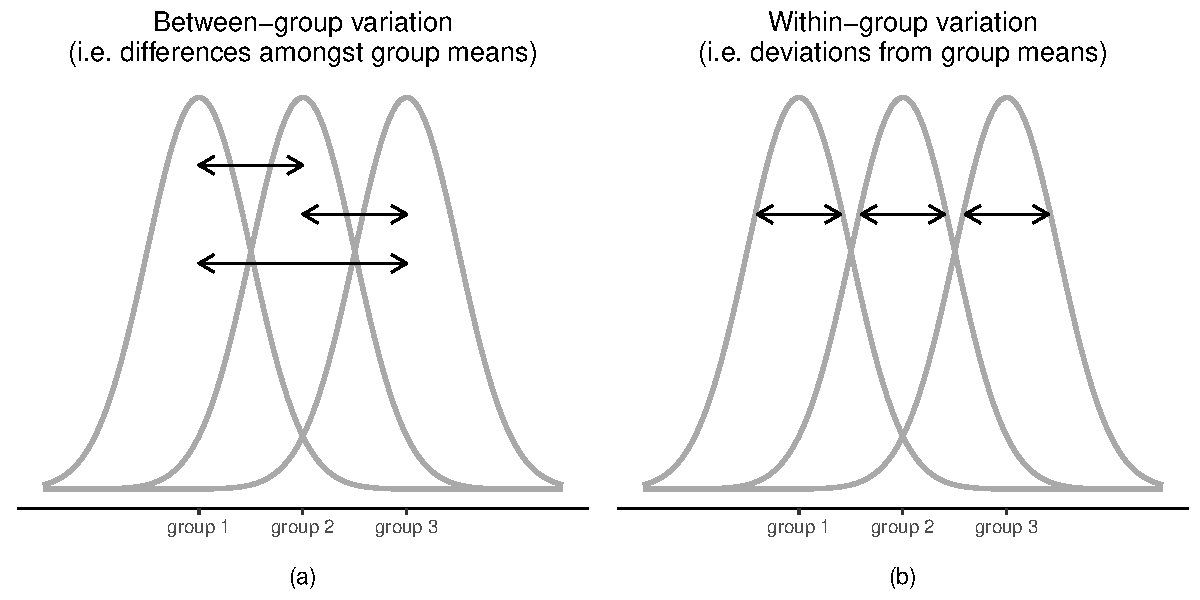
\includegraphics[width=1\textwidth,height=\textheight]{13-Comparing-several-means-one-way-ANOVA_files/figure-pdf/fig-fig13-2-1.pdf} \hfill{}

\caption{\label{fig-fig13-2}Graphical illustration of ``between groups''
variation (panel (a)) and ``within groups'' variation (panel (b)). On
the left the arrows show the differences in the group means. On the
right the arrows highlight the variability within each group}

\end{figure}

\hypertarget{two-formulas-for-the-variance-of-y}{%
\subsection{\texorpdfstring{Two formulas for the variance of
\(Y\)}{Two formulas for the variance of Y}}\label{two-formulas-for-the-variance-of-y}}

First, let's start by introducing some notation. We'll use \(G\) to
refer to the total number of groups. For our data set there are three
drugs, so there are \(G = 3\) groups. Next, we'll use \(N\) to refer to
the total sample size; there are a total of \(N = 18\) people in our
data set. Similarly, let's use \(N_k\) to denote the number of people in
the \(k\)-th group. In our fake clinical trial, the sample size is
\(N_k = 6\) for all three groups.\footnote{When all groups have the same
  number of observations, the experimental design is said to be
  ``balanced''. Balance isn't such a big deal for one-way ANOVA, which
  is the topic of this chapter. It becomes more important when you start
  doing more complicated ANOVAs.} Finally, we'll use \(Y\) to denote the
outcome variable. In our case, \(Y\) refers to mood change.
Specifically, we'll use \(Y_{ik}\) to refer to the mood change
experienced by the \(i\)-th member of the \(k\)-th group. Similarly,
we'll use \(\bar{Y}\) to be the average mood change, taken across all 18
people in the experiment, and \(\bar{Y}_k\) to refer to the average mood
change experienced by the 6 people in group \(k\).

Now that we've got our notation sorted out we can start writing down
formulas. To start with, let's recall the formula for the variance that
we used in \textbf{?@sec-Measures-of-variability}, way back in those
kinder days when we were just doing descriptive statistics. The sample
variance of \(Y\) is defined as follows:
\[Var(Y)=\frac{1}{N}\sum_{k=1}^{G}\sum_{i=1}^{N_k}(Y_{ik}-\bar{Y})^2\]
This formula looks pretty much identical to the formula for the variance
in \textbf{?@sec-Measures-of-variability}. The only difference is that
this time around I've got two summations here: I'm summing over groups
(i.e., values for \(k\)) and over the people within the groups (i.e.,
values for \(i\)). This is purely a cosmetic detail. If I'd instead used
the notation \(Y_p\) to refer to the value of the outcome variable for
person \(p\) in the sample, then I'd only have a single summation. The
only reason that we have a double summation here is that I've classified
people into groups, and then assigned numbers to people within groups.

A concrete example might be useful here. Let's consider
Table~\ref{tbl-tab13-1}, in which we have a total of \(N = 5\) people
sorted into \(G = 2\) groups. Arbitrarily, let's say that the ``cool''
people are group 1 and the ``uncool'' people are group 2. It turns out
that we have three cool people (\(N_1 = 3\)) and two uncool people
(\(N_2 = 2\)).

\hypertarget{tbl-tab13-1}{}
 
  \providecommand{\huxb}[2]{\arrayrulecolor[RGB]{#1}\global\arrayrulewidth=#2pt}
  \providecommand{\huxvb}[2]{\color[RGB]{#1}\vrule width #2pt}
  \providecommand{\huxtpad}[1]{\rule{0pt}{#1}}
  \providecommand{\huxbpad}[1]{\rule[-#1]{0pt}{#1}}

\begin{table}[ht]
\caption{\label{tbl-tab13-1}Grumpiness for people in cool and uncool groups }\tabularnewline

\begin{centerbox}
\begin{threeparttable}
\setlength{\tabcolsep}{0pt}
\begin{tabularx}{0.9\textwidth}{p{0.15\textwidth} p{0.15\textwidth} p{0.15\textwidth} p{0.15\textwidth} p{0.15\textwidth} p{0.15\textwidth}}


\hhline{>{\huxb{0, 0, 0}{0.4}}->{\huxb{0, 0, 0}{0.4}}->{\huxb{0, 0, 0}{0.4}}->{\huxb{0, 0, 0}{0.4}}->{\huxb{0, 0, 0}{0.4}}->{\huxb{0, 0, 0}{0.4}}-}
\arrayrulecolor{black}

\multicolumn{1}{!{\huxvb{0, 0, 0}{0}}p{0.15\textwidth}!{\huxvb{0, 0, 0}{0}}}{\hspace{0pt}\parbox[b]{0.15\textwidth-0pt-12pt}{\huxtpad{2pt + 1em}\centering \textbf{name}\huxbpad{2pt}}} &
\multicolumn{1}{p{0.15\textwidth}!{\huxvb{0, 0, 0}{0}}}{\hspace{12pt}\parbox[b]{0.15\textwidth-12pt-12pt}{\huxtpad{2pt + 1em}\centering \textbf{person \(P\)}\huxbpad{2pt}}} &
\multicolumn{1}{p{0.15\textwidth}!{\huxvb{0, 0, 0}{0}}}{\hspace{12pt}\parbox[b]{0.15\textwidth-12pt-12pt}{\huxtpad{2pt + 1em}\centering \textbf{group}\huxbpad{2pt}}} &
\multicolumn{1}{p{0.15\textwidth}!{\huxvb{0, 0, 0}{0}}}{\hspace{12pt}\parbox[b]{0.15\textwidth-12pt-12pt}{\huxtpad{2pt + 1em}\centering \textbf{group num. \(k\)}\huxbpad{2pt}}} &
\multicolumn{1}{p{0.15\textwidth}!{\huxvb{0, 0, 0}{0}}}{\hspace{12pt}\parbox[b]{0.15\textwidth-12pt-12pt}{\huxtpad{2pt + 1em}\centering \textbf{index in group}\huxbpad{2pt}}} &
\multicolumn{1}{p{0.15\textwidth}!{\huxvb{0, 0, 0}{0}}}{\hspace{12pt}\parbox[b]{0.15\textwidth-12pt-0pt}{\huxtpad{2pt + 1em}\centering \textbf{grumpiness \( Y_{ik} \) or \( Y_p \)}\huxbpad{2pt}}} \tabularnewline[-0.5pt]


\hhline{>{\huxb{0, 0, 0}{0.4}}->{\huxb{0, 0, 0}{0.4}}->{\huxb{0, 0, 0}{0.4}}->{\huxb{0, 0, 0}{0.4}}->{\huxb{0, 0, 0}{0.4}}->{\huxb{0, 0, 0}{0.4}}-}
\arrayrulecolor{black}

\multicolumn{1}{!{\huxvb{0, 0, 0}{0}}p{0.15\textwidth}!{\huxvb{0, 0, 0}{0}}}{\hspace{0pt}\parbox[b]{0.15\textwidth-0pt-12pt}{\huxtpad{2pt + 1em}\centering Ann\huxbpad{2pt}}} &
\multicolumn{1}{p{0.15\textwidth}!{\huxvb{0, 0, 0}{0}}}{\hspace{12pt}\parbox[b]{0.15\textwidth-12pt-12pt}{\huxtpad{2pt + 1em}\centering 1\huxbpad{2pt}}} &
\multicolumn{1}{p{0.15\textwidth}!{\huxvb{0, 0, 0}{0}}}{\hspace{12pt}\parbox[b]{0.15\textwidth-12pt-12pt}{\huxtpad{2pt + 1em}\centering cool\huxbpad{2pt}}} &
\multicolumn{1}{p{0.15\textwidth}!{\huxvb{0, 0, 0}{0}}}{\hspace{12pt}\parbox[b]{0.15\textwidth-12pt-12pt}{\huxtpad{2pt + 1em}\centering 1\huxbpad{2pt}}} &
\multicolumn{1}{p{0.15\textwidth}!{\huxvb{0, 0, 0}{0}}}{\hspace{12pt}\parbox[b]{0.15\textwidth-12pt-12pt}{\huxtpad{2pt + 1em}\centering 1\huxbpad{2pt}}} &
\multicolumn{1}{p{0.15\textwidth}!{\huxvb{0, 0, 0}{0}}}{\hspace{12pt}\parbox[b]{0.15\textwidth-12pt-0pt}{\huxtpad{2pt + 1em}\centering 20\huxbpad{2pt}}} \tabularnewline[-0.5pt]


\hhline{}
\arrayrulecolor{black}

\multicolumn{1}{!{\huxvb{0, 0, 0}{0}}p{0.15\textwidth}!{\huxvb{0, 0, 0}{0}}}{\hspace{0pt}\parbox[b]{0.15\textwidth-0pt-12pt}{\huxtpad{2pt + 1em}\centering Ben\huxbpad{2pt}}} &
\multicolumn{1}{p{0.15\textwidth}!{\huxvb{0, 0, 0}{0}}}{\hspace{12pt}\parbox[b]{0.15\textwidth-12pt-12pt}{\huxtpad{2pt + 1em}\centering 2\huxbpad{2pt}}} &
\multicolumn{1}{p{0.15\textwidth}!{\huxvb{0, 0, 0}{0}}}{\hspace{12pt}\parbox[b]{0.15\textwidth-12pt-12pt}{\huxtpad{2pt + 1em}\centering cool\huxbpad{2pt}}} &
\multicolumn{1}{p{0.15\textwidth}!{\huxvb{0, 0, 0}{0}}}{\hspace{12pt}\parbox[b]{0.15\textwidth-12pt-12pt}{\huxtpad{2pt + 1em}\centering 1\huxbpad{2pt}}} &
\multicolumn{1}{p{0.15\textwidth}!{\huxvb{0, 0, 0}{0}}}{\hspace{12pt}\parbox[b]{0.15\textwidth-12pt-12pt}{\huxtpad{2pt + 1em}\centering 2\huxbpad{2pt}}} &
\multicolumn{1}{p{0.15\textwidth}!{\huxvb{0, 0, 0}{0}}}{\hspace{12pt}\parbox[b]{0.15\textwidth-12pt-0pt}{\huxtpad{2pt + 1em}\centering 55\huxbpad{2pt}}} \tabularnewline[-0.5pt]


\hhline{}
\arrayrulecolor{black}

\multicolumn{1}{!{\huxvb{0, 0, 0}{0}}p{0.15\textwidth}!{\huxvb{0, 0, 0}{0}}}{\hspace{0pt}\parbox[b]{0.15\textwidth-0pt-12pt}{\huxtpad{2pt + 1em}\centering Cat\huxbpad{2pt}}} &
\multicolumn{1}{p{0.15\textwidth}!{\huxvb{0, 0, 0}{0}}}{\hspace{12pt}\parbox[b]{0.15\textwidth-12pt-12pt}{\huxtpad{2pt + 1em}\centering 3\huxbpad{2pt}}} &
\multicolumn{1}{p{0.15\textwidth}!{\huxvb{0, 0, 0}{0}}}{\hspace{12pt}\parbox[b]{0.15\textwidth-12pt-12pt}{\huxtpad{2pt + 1em}\centering cool\huxbpad{2pt}}} &
\multicolumn{1}{p{0.15\textwidth}!{\huxvb{0, 0, 0}{0}}}{\hspace{12pt}\parbox[b]{0.15\textwidth-12pt-12pt}{\huxtpad{2pt + 1em}\centering 1\huxbpad{2pt}}} &
\multicolumn{1}{p{0.15\textwidth}!{\huxvb{0, 0, 0}{0}}}{\hspace{12pt}\parbox[b]{0.15\textwidth-12pt-12pt}{\huxtpad{2pt + 1em}\centering 3\huxbpad{2pt}}} &
\multicolumn{1}{p{0.15\textwidth}!{\huxvb{0, 0, 0}{0}}}{\hspace{12pt}\parbox[b]{0.15\textwidth-12pt-0pt}{\huxtpad{2pt + 1em}\centering 21\huxbpad{2pt}}} \tabularnewline[-0.5pt]


\hhline{}
\arrayrulecolor{black}

\multicolumn{1}{!{\huxvb{0, 0, 0}{0}}p{0.15\textwidth}!{\huxvb{0, 0, 0}{0}}}{\hspace{0pt}\parbox[b]{0.15\textwidth-0pt-12pt}{\huxtpad{2pt + 1em}\centering Tim\huxbpad{2pt}}} &
\multicolumn{1}{p{0.15\textwidth}!{\huxvb{0, 0, 0}{0}}}{\hspace{12pt}\parbox[b]{0.15\textwidth-12pt-12pt}{\huxtpad{2pt + 1em}\centering 4\huxbpad{2pt}}} &
\multicolumn{1}{p{0.15\textwidth}!{\huxvb{0, 0, 0}{0}}}{\hspace{12pt}\parbox[b]{0.15\textwidth-12pt-12pt}{\huxtpad{2pt + 1em}\centering uncool\huxbpad{2pt}}} &
\multicolumn{1}{p{0.15\textwidth}!{\huxvb{0, 0, 0}{0}}}{\hspace{12pt}\parbox[b]{0.15\textwidth-12pt-12pt}{\huxtpad{2pt + 1em}\centering 2\huxbpad{2pt}}} &
\multicolumn{1}{p{0.15\textwidth}!{\huxvb{0, 0, 0}{0}}}{\hspace{12pt}\parbox[b]{0.15\textwidth-12pt-12pt}{\huxtpad{2pt + 1em}\centering 1\huxbpad{2pt}}} &
\multicolumn{1}{p{0.15\textwidth}!{\huxvb{0, 0, 0}{0}}}{\hspace{12pt}\parbox[b]{0.15\textwidth-12pt-0pt}{\huxtpad{2pt + 1em}\centering 91\huxbpad{2pt}}} \tabularnewline[-0.5pt]


\hhline{}
\arrayrulecolor{black}

\multicolumn{1}{!{\huxvb{0, 0, 0}{0}}p{0.15\textwidth}!{\huxvb{0, 0, 0}{0}}}{\hspace{0pt}\parbox[b]{0.15\textwidth-0pt-12pt}{\huxtpad{2pt + 1em}\centering Egg\huxbpad{2pt}}} &
\multicolumn{1}{p{0.15\textwidth}!{\huxvb{0, 0, 0}{0}}}{\hspace{12pt}\parbox[b]{0.15\textwidth-12pt-12pt}{\huxtpad{2pt + 1em}\centering 5\huxbpad{2pt}}} &
\multicolumn{1}{p{0.15\textwidth}!{\huxvb{0, 0, 0}{0}}}{\hspace{12pt}\parbox[b]{0.15\textwidth-12pt-12pt}{\huxtpad{2pt + 1em}\centering uncool\huxbpad{2pt}}} &
\multicolumn{1}{p{0.15\textwidth}!{\huxvb{0, 0, 0}{0}}}{\hspace{12pt}\parbox[b]{0.15\textwidth-12pt-12pt}{\huxtpad{2pt + 1em}\centering 2\huxbpad{2pt}}} &
\multicolumn{1}{p{0.15\textwidth}!{\huxvb{0, 0, 0}{0}}}{\hspace{12pt}\parbox[b]{0.15\textwidth-12pt-12pt}{\huxtpad{2pt + 1em}\centering 2\huxbpad{2pt}}} &
\multicolumn{1}{p{0.15\textwidth}!{\huxvb{0, 0, 0}{0}}}{\hspace{12pt}\parbox[b]{0.15\textwidth-12pt-0pt}{\huxtpad{2pt + 1em}\centering 22\huxbpad{2pt}}} \tabularnewline[-0.5pt]


\hhline{>{\huxb{0, 0, 0}{0.4}}->{\huxb{0, 0, 0}{0.4}}->{\huxb{0, 0, 0}{0.4}}->{\huxb{0, 0, 0}{0.4}}->{\huxb{0, 0, 0}{0.4}}->{\huxb{0, 0, 0}{0.4}}-}
\arrayrulecolor{black}
\end{tabularx} 

\end{threeparttable}\par\end{centerbox}

\end{table}
 

Notice that I've constructed two different labelling schemes here. We
have a ``person'' variable \(p\) so it would be perfectly sensible to
refer to \(Y_p\) as the grumpiness of the \(p\)-th person in the sample.
For instance, the table shows that Tim is the fourth so we'd say
\(p = 4\). So, when talking about the grumpiness \(Y\) of this ``Tim''
person, whoever he might be, we could refer to his grumpiness by saying
that \(Y_p = 91\), for person \(p = 4\) that is. However, that's not the
only way we could refer to Tim. As an alternative we could note that Tim
belongs to the ``uncool'' group (\(k = 2\)), and is in fact the first
person listed in the uncool group (\(i = 1\)). So it's equally valid to
refer to Tim's grumpiness by saying that \(Y_{ik} = 91\), where
\(k = 2\) and \(i = 1\).

In other words, each person \(p\) corresponds to a unique \(ik\)
combination, and so the formula that I gave above is actually identical
to our original formula for the variance, which would be
\[Var(Y)=\frac{1}{N}\sum_{p=1}^{N}(Y_p-\bar{Y})^2\] In both formulas,
all we're doing is summing over all of the observations in the sample.
Most of the time we would just use the simpler \(Y_p\) notation; the
equation using \(Y_p\) is clearly the simpler of the two. However, when
doing an ANOVA it's important to keep track of which participants belong
in which groups, and we need to use the \(Y_{ik}\) notation to do this.

\hypertarget{from-variances-to-sums-of-squares}{%
\subsection{From variances to sums of
squares}\label{from-variances-to-sums-of-squares}}

Okay, now that we've got a good grasp on how the variance is calculated,
let's define something called the \textbf{total sum of squares}, which
is denoted \(SStot\). This is very simple. Instead of averaging the
squared deviations, which is what we do when calculating the variance,
we just add them up.\footnote{So the formula for the total sum of
  squares is almost identical to the formula for the variance
  \[SS_{tot}=\sum_{k=1}^{G} \sum_{i=1}^{N_k} (Y_{ik} - \bar{Y})^2\]}

When we talk about analysing variances in the context of ANOVA, what
we're really doing is working with the total sums of squares rather than
the actual variance.\footnote{One very nice thing about the total sum of
  squares is that we can break it up into two different kinds of
  variation First, we can talk about the within-group sum of squares, in
  which we look to see how different each individual person is from
  their own group mean
  \[SS_{w}= \sum_{k=1}^{G} \sum_{i=1}^{N_k} (Y_{ik} - \bar{Y}_k)^2\]
  where \(\bar{Y}_k\) is a group mean. In our example, \(\bar{Y}_k\)
  would be the average mood change experienced by those people given the
  k-th drug. So, instead of comparing individuals to the average of all
  people in the experiment, we're only comparing them to those people in
  the the same group. As a consequence, you'd expect the value of
  \(SS_w\) to be smaller than the total sum of squares, because it's
  completely ignoring any group differences, i.e., whether the drugs
  will have different effects on people's moods.}

Next, we can define a third notion of variation which captures only the
differences between groups. We do this by looking at the differences
between the group means \(\bar{Y}_k\) and grand mean
\(\bar{Y}\).\footnote{In order to quantify the extent of this variation,
  what we do is calculate the between-group sum of squares
  \[\begin{aligned} SS_{b} &= \sum_{k=1}^{G} \sum_{i=1}^{N_k} ( \bar{Y}_{k} - \bar{Y} )^2 \\ &= \sum_{k=1}^{G} N_k ( \bar{Y}_{k} - \bar{Y} )^2 \end{aligned}\]}

It's not too difficult to show that the total variation among people in
the experiment \(SS_{tot}\) is actually the sum of the differences
between the groups \(SS_b\) and the variation inside the groups
\(SS_w\). That is,

\[SS_w+SS_b=SS_{tot}\]

Okay, so what have we found out? We've discovered that the total
variability associated with the outcome variable (\(SS_{tot}\)) can be
mathematically carved up into the sum of ``the variation due to the
differences in the sample means for the different groups'' (\(SS_b\))
plus ``all the rest of the variation'' (\(SS_w\)).\footnote{\(SS_w\) is
  also referred to in an independent ANOVA as the error variance, or
  \(SS_{error}\).}

How does that help me find out whether the groups have different
population means? Um. Wait. Hold on a second. Now that I think about it,
this is exactly what we were looking for. If the null hypothesis is true
then you'd expect all the sample means to be pretty similar to each
other, right? And that would imply that you'd expect \(SS_b\) to be
really small, or at least you'd expect it to be a lot smaller than ``the
variation associated with everything else'', \(SS_w\). Hmm. I detect a
hypothesis test coming on.

\hypertarget{from-sums-of-squares-to-the-f-test}{%
\subsection{From sums of squares to the
F-test}\label{from-sums-of-squares-to-the-f-test}}

As we saw in the last section, the qualitative idea behind ANOVA is to
compare the two sums of squares values \(SS_b\) and \(SS_w\) to each
other. If the between-group variation \(SS_b\) is large relative to the
within-group variation \(SS_w\) then we have reason to suspect that the
population means for the different groups aren't identical to each
other. In order to convert this into a workable hypothesis test, there's
a little bit of ``fiddling around'' needed. What I'll do is first show
you what we do to calculate our test statistic, the
\textbf{\(F\)-ratio}, and then try to give you a feel for why we do it
this way.

In order to convert our \(SS\) values into an \(F\)-ratio the first
thing we need to calculate is the \textbf{degrees of freedom} associated
with the \(SS_b\) and \(SS_w\) values. As usual, the degrees of freedom
corresponds to the number of unique ``data points'' that contribute to a
particular calculation, minus the number of ``constraints'' that they
need to satisfy. For the within groups variability what we're
calculating is the variation of the individual observations (\(N\) data
points) around the group means (\(G\) constraints). In contrast, for the
between groups variability we're interested in the variation of the
group means (\(G\) data points) around the grand mean (1 constraint).
Therefore, the degrees of freedom here are:

\[df_b=G-1\] \[df_w=N-G\]

Okay, that seems simple enough. What we do next is convert our summed
squares value into a ``mean squares'' value, which we do by dividing by
the degrees of freedom:

\[MS_b=\frac{SS_b}{df_b}\] \[MS_w=\frac{SS_w}{df_w}\]

Finally, we calculate the \(F\)-ratio by dividing the between groups
\(MS\) by the within groups \(MS\):

\[F=\frac{MS_b}{MS_w}\]

At a very general level, the intuition behind the \(F\) statistic is
straightforward. Bigger values of \(F\) means that the between groups
variation is large relative to the within groups variation. As a
consequence, the larger the value of \(F\) the more evidence we have
against the null hypothesis. But how large does \(F\) have to be in
order to actually reject \(H_0\)? In order to understand this, you need
a slightly deeper understanding of what ANOVA is and what the mean
squares values actually are.

The next section discusses that in a bit of detail, but for readers that
aren't interested in the details of what the test is actually measuring
I'll cut to the chase. In order to complete our hypothesis test we need
to know the sampling distribution for \(F\) if the null hypothesis is
true. Not surprisingly, the sampling distribution for the \(F\)
statistic under the null hypothesis is an \(F\) distribution. If you
recall our discussion of the \(F\) distribution in
\textbf{?@sec-Introduction-to-probability}, the \(F\) distribution has
two parameters, corresponding to the two degrees of freedom involved.
The first one \(df_1\) is the between groups degrees of freedom
\(df_b\), and the second one \(df_2\) is the within groups degrees of
freedom \(df_w\).

\hypertarget{tbl-tab13-2}{}
 
  \providecommand{\huxb}[2]{\arrayrulecolor[RGB]{#1}\global\arrayrulewidth=#2pt}
  \providecommand{\huxvb}[2]{\color[RGB]{#1}\vrule width #2pt}
  \providecommand{\huxtpad}[1]{\rule{0pt}{#1}}
  \providecommand{\huxbpad}[1]{\rule[-#1]{0pt}{#1}}

\begin{table}[ht]
\caption{\label{tbl-tab13-2}All of the key quantities involved in an ANOVA organised into a
``standard'' ANOVA table. The formulas for all quantities (except the
\(p\)-value which has a very ugly formula and would be nightmarishly
hard to calculate without a computer) are shown }\tabularnewline

\begin{centerbox}
\begin{threeparttable}
\setlength{\tabcolsep}{0pt}
\begin{tabularx}{0.9\textwidth}{p{0.3\textwidth} p{0.3\textwidth} p{0.3\textwidth}}


\hhline{>{\huxb{0, 0, 0}{0.4}}->{\huxb{0, 0, 0}{0.4}}->{\huxb{0, 0, 0}{0.4}}-}
\arrayrulecolor{black}

\multicolumn{1}{!{\huxvb{0, 0, 0}{0}}p{0.3\textwidth}!{\huxvb{0, 0, 0}{0}}}{\hspace{0pt}\parbox[b]{0.3\textwidth-0pt-12pt}{\huxtpad{2pt + 1em}\centering \textbf{}\huxbpad{2pt}}} &
\multicolumn{1}{p{0.3\textwidth}!{\huxvb{0, 0, 0}{0}}}{\hspace{12pt}\parbox[b]{0.3\textwidth-12pt-12pt}{\huxtpad{2pt + 1em}\centering \textbf{between
groups}\huxbpad{2pt}}} &
\multicolumn{1}{p{0.3\textwidth}!{\huxvb{0, 0, 0}{0}}}{\hspace{12pt}\parbox[b]{0.3\textwidth-12pt-0pt}{\huxtpad{2pt + 1em}\centering \textbf{within
groups}\huxbpad{2pt}}} \tabularnewline[-0.5pt]


\hhline{>{\huxb{0, 0, 0}{0.4}}->{\huxb{0, 0, 0}{0.4}}->{\huxb{0, 0, 0}{0.4}}-}
\arrayrulecolor{black}

\multicolumn{1}{!{\huxvb{0, 0, 0}{0}}p{0.3\textwidth}!{\huxvb{0, 0, 0}{0}}}{\hspace{0pt}\parbox[b]{0.3\textwidth-0pt-12pt}{\huxtpad{2pt + 1em}\centering \( df \)\huxbpad{2pt}}} &
\multicolumn{1}{p{0.3\textwidth}!{\huxvb{0, 0, 0}{0}}}{\hspace{12pt}\parbox[b]{0.3\textwidth-12pt-12pt}{\huxtpad{2pt + 1em}\centering \(  df_b=G-1  \)\huxbpad{2pt}}} &
\multicolumn{1}{p{0.3\textwidth}!{\huxvb{0, 0, 0}{0}}}{\hspace{12pt}\parbox[b]{0.3\textwidth-12pt-0pt}{\huxtpad{2pt + 1em}\centering \(  df_w=N-G  \)\huxbpad{2pt}}} \tabularnewline[-0.5pt]


\hhline{}
\arrayrulecolor{black}

\multicolumn{1}{!{\huxvb{0, 0, 0}{0}}p{0.3\textwidth}!{\huxvb{0, 0, 0}{0}}}{\hspace{0pt}\parbox[b]{0.3\textwidth-0pt-12pt}{\huxtpad{2pt + 1em}\centering sum of squares\huxbpad{2pt}}} &
\multicolumn{1}{p{0.3\textwidth}!{\huxvb{0, 0, 0}{0}}}{\hspace{12pt}\parbox[b]{0.3\textwidth-12pt-12pt}{\huxtpad{2pt + 1em}\centering \(  SS_b=\sum_{k=1}^{G} N_k  (\bar{Y}_k-\bar{Y})^2  \)\huxbpad{2pt}}} &
\multicolumn{1}{p{0.3\textwidth}!{\huxvb{0, 0, 0}{0}}}{\hspace{12pt}\parbox[b]{0.3\textwidth-12pt-0pt}{\huxtpad{2pt + 1em}\centering \(  SS_w=\sum_{k=1}^{G} \sum_{i=1}^{N_k}   (Y_{ik}-\bar{Y}_k)^2  \)\huxbpad{2pt}}} \tabularnewline[-0.5pt]


\hhline{}
\arrayrulecolor{black}

\multicolumn{1}{!{\huxvb{0, 0, 0}{0}}p{0.3\textwidth}!{\huxvb{0, 0, 0}{0}}}{\hspace{0pt}\parbox[b]{0.3\textwidth-0pt-12pt}{\huxtpad{2pt + 1em}\centering mean squares\huxbpad{2pt}}} &
\multicolumn{1}{p{0.3\textwidth}!{\huxvb{0, 0, 0}{0}}}{\hspace{12pt}\parbox[b]{0.3\textwidth-12pt-12pt}{\huxtpad{2pt + 1em}\centering \(  MS_b=\frac{SS_b}{df_b}  \)\huxbpad{2pt}}} &
\multicolumn{1}{p{0.3\textwidth}!{\huxvb{0, 0, 0}{0}}}{\hspace{12pt}\parbox[b]{0.3\textwidth-12pt-0pt}{\huxtpad{2pt + 1em}\centering \(  MS_w=\frac{SS_w}{df_w}  \)\huxbpad{2pt}}} \tabularnewline[-0.5pt]


\hhline{}
\arrayrulecolor{black}

\multicolumn{1}{!{\huxvb{0, 0, 0}{0}}p{0.3\textwidth}!{\huxvb{0, 0, 0}{0}}}{\hspace{0pt}\parbox[b]{0.3\textwidth-0pt-12pt}{\huxtpad{2pt + 1em}\centering \( F \)-statistic\huxbpad{2pt}}} &
\multicolumn{1}{p{0.3\textwidth}!{\huxvb{0, 0, 0}{0}}}{\hspace{12pt}\parbox[b]{0.3\textwidth-12pt-12pt}{\huxtpad{2pt + 1em}\centering \(  F=\frac{MS_b}{df_b}  \)\huxbpad{2pt}}} &
\multicolumn{1}{p{0.3\textwidth}!{\huxvb{0, 0, 0}{0}}}{\hspace{12pt}\parbox[b]{0.3\textwidth-12pt-0pt}{\huxtpad{2pt + 1em}\centering -\huxbpad{2pt}}} \tabularnewline[-0.5pt]


\hhline{}
\arrayrulecolor{black}

\multicolumn{1}{!{\huxvb{0, 0, 0}{0}}p{0.3\textwidth}!{\huxvb{0, 0, 0}{0}}}{\hspace{0pt}\parbox[b]{0.3\textwidth-0pt-12pt}{\huxtpad{2pt + 1em}\centering \(p\)-value\huxbpad{2pt}}} &
\multicolumn{1}{p{0.3\textwidth}!{\huxvb{0, 0, 0}{0}}}{\hspace{12pt}\parbox[b]{0.3\textwidth-12pt-12pt}{\huxtpad{2pt + 1em}\centering [complicated]\huxbpad{2pt}}} &
\multicolumn{1}{p{0.3\textwidth}!{\huxvb{0, 0, 0}{0}}}{\hspace{12pt}\parbox[b]{0.3\textwidth-12pt-0pt}{\huxtpad{2pt + 1em}\centering -\huxbpad{2pt}}} \tabularnewline[-0.5pt]


\hhline{>{\huxb{0, 0, 0}{0.4}}->{\huxb{0, 0, 0}{0.4}}->{\huxb{0, 0, 0}{0.4}}-}
\arrayrulecolor{black}
\end{tabularx} 

\end{threeparttable}\par\end{centerbox}

\end{table}
 

A summary of all the key quantities involved in a one-way ANOVA,
including the formulas showing how they are calculated, is shown in
Table~\ref{tbl-tab13-2}.

{[}Additional technical detail\footnote{At a fundamental level ANOVA is
  a competition between two different statistical models, \(H_0\) and
  \(H_1\). When I described the null and alternative hypotheses at the
  start of the section, I was a little imprecise about what these models
  actually are. I'll remedy that now, though you probably won't like me
  for doing so. If you recall, our null hypothesis was that all of the
  group means are identical to one another. If so, then a natural way to
  think about the outcome variable \(Y_{ik}\) is to describe individual
  scores in terms of a single population mean \(\mu\), plus the
  deviation from that population mean. This deviation is usually denoted
  \(\epsilon_{ik}\) and is traditionally called the error or residual
  associated with that observation. Be careful though. Just like we saw
  with the word ``significant'', the word ``error'' has a technical
  meaning in statistics that isn't quite the same as its everyday
  English definition. In everyday language, ``error'' implies a mistake
  of some kind, but in statistics it doesn't (or at least, not
  necessarily). With that in mind, the word ``residual'' is a better
  term than the word ``error''. In statistics both words mean ``leftover
  variability'', that is ``stuff'' that the model can't explain. In any
  case, here's what the null hypothesis looks like when we write it as a
  statistical model \[Y_{ik}=\mu+\epsilon_{ik}\] where we make the
  assumption (discussed later) that the residual values
  \(\epsilon_{ik}\) are normally distributed, with mean \(0\) and a
  standard deviation \(\sigma\) that is the same for all groups. To use
  the notation that we introduced in the {[}Introduction to
  probability{]} we would write this assumption like this
  \[\epsilon_{ik} \sim Normal(0,\sigma^2)\] What about the alternative
  hypothesis, \(H_1\)? The only difference between the null hypothesis
  and the alternative hypothesis is that we allow each group to have a
  different population mean. So, if we let \(\mu_k\) denote the
  population mean for the k-th group in our experiment, then the
  statistical model corresponding to \(H_1\) is
  \[Y_{ik}=\mu_k+\epsilon_{ik}\] where, once again, we assume that the
  error terms are normally distributed with mean 0 and standard
  deviation \(\sigma\). That is, the alternative hypothesis also assumes
  that \(\epsilon \sim Normal(0,\sigma^2)\) Okay, now that we've
  described the statistical models underpinning \(H_0\) and \(H_1\) in
  more detail, it's now pretty straightforward to say what the mean
  square values are measuring, and what this means for the
  interpretation of \(F\). I won't bore you with the proof of this but
  it turns out that the within-groups mean square, \(MS_w\), can be
  viewed as an estimator of the error variance \(\sigma^2\) . The
  between-groups mean square \(MS_b\) is also an estimator, but what it
  estimates is the error variance plus a quantity that depends on the
  true differences among the group means. If we call this quantity
  \(Q\), then we can see that the \(F\) statistic is basically\(^a\)
  \[F=\frac{\hat{Q}+\hat{\sigma}^2}{\hat{\sigma}^2}\] where the true
  value \(Q = 0\) if the null hypothesis is true, and \(Q < 0\) if the
  alternative hypothesis is true (e.g., Hays (1994), ch.~10). Therefore,
  at a bare minimum the \(F\) \emph{value must be larger than} 1 to have
  any chance of rejecting the null hypothesis. Note that this doesn't
  mean that it's impossible to get an \(F\)-value less than 1. What it
  means is that if the null hypothesis is true the sampling distribution
  of the \(F\)-ratio has a mean of 1,{[}\^{}b{]} and so we need to see
  \(F\)-values larger than 1 in order to safely reject the null. To be a
  bit more precise about the sampling distribution, notice that if the
  null hypothesis is true, both \(MS\)b and \(MSw\) are estimators of
  the variance of the residuals \(\epsilon_{ik}\). If those residuals
  are normally distributed, then you might suspect that the estimate of
  the variance of \(\epsilon_{ik}\) is chi-square distributed, because
  (as discussed in the \textbf{?@sec-Other-useful-distributions}) that's
  what a chi-square distribution is: it's what you get when you square a
  bunch of normally-distributed things and add them up. And since the
  \(F\) distribution is (again, by definition) what you get when you
  take the ratio between two things that are \(\chi^2\) distributed, we
  have our sampling distribution. Obviously, I'm glossing over a whole
  lot of stuff when I say this, but in broad terms, this really is where
  our sampling distribution comes from. --- \(^a\)If you read ahead to
  Chapter~\ref{sec-Factorial-ANOVA} and look at how the ``treatment
  effect'' at level \(k\) of a factor is defined in terms of the
  \(\alpha_k\) values (see {[}Factorial ANOVA 2: balanced designs,
  interactions allowed{]}), it turns out that \(Q\) refers to a weighted
  mean of the squared treatment effects,
  \(Q = \frac{(\sum_{k=1}^{G}N_k \alpha_k^2)}{(G-1)}\). --- \(^b\)Or, if
  we want to be sticklers for accuracy, \(1+ \frac{2}{df_2-2}\).}{]}

\hypertarget{a-worked-example}{%
\subsection{A worked example}\label{a-worked-example}}

The previous discussion was fairly abstract and a little on the
technical side, so I think that at this point it might be useful to see
a worked example. For that, let's go back to the clinical trial data
that I introduced at the start of the chapter. The descriptive
statistics that we calculated at the beginning tell us our group means:
an average mood gain of \(0.45\) for the placebo, \(0.72\) for Anxifree,
and \(1.48\) for Joyzepam. With that in mind, let's party like it's
1899\footnote{Or, to be precise, party like ``it's 1899 and we've got no
  friends and nothing better to do with our time than do some
  calculations that wouldn't have made any sense in 1899 because ANOVA
  didn't exist until about the 1920s''.} and start doing some pencil and
paper calculations. I'll only do this for the first \(5\) observations
because it's not bloody \(1899\) and I'm very lazy. Let's start by
calculating \(SS_w\), the within-group sums of squares. First, let's
draw up a nice table to help us with our calculations
(Table~\ref{tbl-tab13-3})

\hypertarget{tbl-tab13-3}{}
 
  \providecommand{\huxb}[2]{\arrayrulecolor[RGB]{#1}\global\arrayrulewidth=#2pt}
  \providecommand{\huxvb}[2]{\color[RGB]{#1}\vrule width #2pt}
  \providecommand{\huxtpad}[1]{\rule{0pt}{#1}}
  \providecommand{\huxbpad}[1]{\rule[-#1]{0pt}{#1}}

\begin{table}[ht]
\caption{\label{tbl-tab13-3}A worked example\ldots1 }\tabularnewline

\begin{centerbox}
\begin{threeparttable}
\setlength{\tabcolsep}{0pt}
\begin{tabularx}{0.9\textwidth}{p{0.45\textwidth} p{0.45\textwidth}}


\hhline{>{\huxb{0, 0, 0}{0.4}}->{\huxb{0, 0, 0}{0.4}}-}
\arrayrulecolor{black}

\multicolumn{1}{!{\huxvb{0, 0, 0}{0}}p{0.45\textwidth}!{\huxvb{0, 0, 0}{0}}}{\hspace{0pt}\parbox[b]{0.45\textwidth-0pt-12pt}{\huxtpad{2pt + 1em}\centering \textbf{group \( k \)}\huxbpad{2pt}}} &
\multicolumn{1}{p{0.45\textwidth}!{\huxvb{0, 0, 0}{0}}}{\hspace{12pt}\parbox[b]{0.45\textwidth-12pt-0pt}{\huxtpad{2pt + 1em}\centering \textbf{outcome \( Y_{ik} \)}\huxbpad{2pt}}} \tabularnewline[-0.5pt]


\hhline{>{\huxb{0, 0, 0}{0.4}}->{\huxb{0, 0, 0}{0.4}}-}
\arrayrulecolor{black}

\multicolumn{1}{!{\huxvb{0, 0, 0}{0}}p{0.45\textwidth}!{\huxvb{0, 0, 0}{0}}}{\hspace{0pt}\parbox[b]{0.45\textwidth-0pt-12pt}{\huxtpad{2pt + 1em}\centering placebo\huxbpad{2pt}}} &
\multicolumn{1}{p{0.45\textwidth}!{\huxvb{0, 0, 0}{0}}}{\hspace{12pt}\parbox[b]{0.45\textwidth-12pt-0pt}{\huxtpad{2pt + 1em}\centering 0.5\huxbpad{2pt}}} \tabularnewline[-0.5pt]


\hhline{}
\arrayrulecolor{black}

\multicolumn{1}{!{\huxvb{0, 0, 0}{0}}p{0.45\textwidth}!{\huxvb{0, 0, 0}{0}}}{\hspace{0pt}\parbox[b]{0.45\textwidth-0pt-12pt}{\huxtpad{2pt + 1em}\centering placebo\huxbpad{2pt}}} &
\multicolumn{1}{p{0.45\textwidth}!{\huxvb{0, 0, 0}{0}}}{\hspace{12pt}\parbox[b]{0.45\textwidth-12pt-0pt}{\huxtpad{2pt + 1em}\centering 0.3\huxbpad{2pt}}} \tabularnewline[-0.5pt]


\hhline{}
\arrayrulecolor{black}

\multicolumn{1}{!{\huxvb{0, 0, 0}{0}}p{0.45\textwidth}!{\huxvb{0, 0, 0}{0}}}{\hspace{0pt}\parbox[b]{0.45\textwidth-0pt-12pt}{\huxtpad{2pt + 1em}\centering placebo\huxbpad{2pt}}} &
\multicolumn{1}{p{0.45\textwidth}!{\huxvb{0, 0, 0}{0}}}{\hspace{12pt}\parbox[b]{0.45\textwidth-12pt-0pt}{\huxtpad{2pt + 1em}\centering 0.1\huxbpad{2pt}}} \tabularnewline[-0.5pt]


\hhline{}
\arrayrulecolor{black}

\multicolumn{1}{!{\huxvb{0, 0, 0}{0}}p{0.45\textwidth}!{\huxvb{0, 0, 0}{0}}}{\hspace{0pt}\parbox[b]{0.45\textwidth-0pt-12pt}{\huxtpad{2pt + 1em}\centering anxifree\huxbpad{2pt}}} &
\multicolumn{1}{p{0.45\textwidth}!{\huxvb{0, 0, 0}{0}}}{\hspace{12pt}\parbox[b]{0.45\textwidth-12pt-0pt}{\huxtpad{2pt + 1em}\centering 0.6\huxbpad{2pt}}} \tabularnewline[-0.5pt]


\hhline{}
\arrayrulecolor{black}

\multicolumn{1}{!{\huxvb{0, 0, 0}{0}}p{0.45\textwidth}!{\huxvb{0, 0, 0}{0}}}{\hspace{0pt}\parbox[b]{0.45\textwidth-0pt-12pt}{\huxtpad{2pt + 1em}\centering anxifree\huxbpad{2pt}}} &
\multicolumn{1}{p{0.45\textwidth}!{\huxvb{0, 0, 0}{0}}}{\hspace{12pt}\parbox[b]{0.45\textwidth-12pt-0pt}{\huxtpad{2pt + 1em}\centering 0.4\huxbpad{2pt}}} \tabularnewline[-0.5pt]


\hhline{>{\huxb{0, 0, 0}{0.4}}->{\huxb{0, 0, 0}{0.4}}-}
\arrayrulecolor{black}
\end{tabularx} 

\end{threeparttable}\par\end{centerbox}

\end{table}
 

At this stage, the only thing I've included in the table is the raw data
itself. That is, the grouping variable (i.e., drug) and outcome variable
(i.e.~mood.gain) for each person. Note that the outcome variable here
corresponds to the \(\bar{Y}_{ik}\) value in our equation previously.
The next step in the calculation is to write down, for each person in
the study, the corresponding group mean, \(\bar{Y}_k\). This is slightly
repetitive but not particularly difficult since we already calculated
those group means when doing our descriptive statistics, see
Table~\ref{tbl-tab13-4}.

\hypertarget{tbl-tab13-4}{}
 
  \providecommand{\huxb}[2]{\arrayrulecolor[RGB]{#1}\global\arrayrulewidth=#2pt}
  \providecommand{\huxvb}[2]{\color[RGB]{#1}\vrule width #2pt}
  \providecommand{\huxtpad}[1]{\rule{0pt}{#1}}
  \providecommand{\huxbpad}[1]{\rule[-#1]{0pt}{#1}}

\begin{table}[ht]
\caption{\label{tbl-tab13-4}A worked example\ldots2 }\tabularnewline

\begin{centerbox}
\begin{threeparttable}
\setlength{\tabcolsep}{0pt}
\begin{tabularx}{0.9\textwidth}{p{0.3\textwidth} p{0.3\textwidth} p{0.3\textwidth}}


\hhline{>{\huxb{0, 0, 0}{0.4}}->{\huxb{0, 0, 0}{0.4}}->{\huxb{0, 0, 0}{0.4}}-}
\arrayrulecolor{black}

\multicolumn{1}{!{\huxvb{0, 0, 0}{0}}p{0.3\textwidth}!{\huxvb{0, 0, 0}{0}}}{\hspace{0pt}\parbox[b]{0.3\textwidth-0pt-12pt}{\huxtpad{2pt + 1em}\centering \textbf{group \( k \)}\huxbpad{2pt}}} &
\multicolumn{1}{p{0.3\textwidth}!{\huxvb{0, 0, 0}{0}}}{\hspace{12pt}\parbox[b]{0.3\textwidth-12pt-12pt}{\huxtpad{2pt + 1em}\centering \textbf{outcome \( Y_{ik} \)}\huxbpad{2pt}}} &
\multicolumn{1}{p{0.3\textwidth}!{\huxvb{0, 0, 0}{0}}}{\hspace{12pt}\parbox[b]{0.3\textwidth-12pt-0pt}{\huxtpad{2pt + 1em}\centering \textbf{group mean \( \bar{Y}_k \)}\huxbpad{2pt}}} \tabularnewline[-0.5pt]


\hhline{>{\huxb{0, 0, 0}{0.4}}->{\huxb{0, 0, 0}{0.4}}->{\huxb{0, 0, 0}{0.4}}-}
\arrayrulecolor{black}

\multicolumn{1}{!{\huxvb{0, 0, 0}{0}}p{0.3\textwidth}!{\huxvb{0, 0, 0}{0}}}{\hspace{0pt}\parbox[b]{0.3\textwidth-0pt-12pt}{\huxtpad{2pt + 1em}\centering placebo\huxbpad{2pt}}} &
\multicolumn{1}{p{0.3\textwidth}!{\huxvb{0, 0, 0}{0}}}{\hspace{12pt}\parbox[b]{0.3\textwidth-12pt-12pt}{\huxtpad{2pt + 1em}\centering 0.5\huxbpad{2pt}}} &
\multicolumn{1}{p{0.3\textwidth}!{\huxvb{0, 0, 0}{0}}}{\hspace{12pt}\parbox[b]{0.3\textwidth-12pt-0pt}{\huxtpad{2pt + 1em}\centering 0.45\huxbpad{2pt}}} \tabularnewline[-0.5pt]


\hhline{}
\arrayrulecolor{black}

\multicolumn{1}{!{\huxvb{0, 0, 0}{0}}p{0.3\textwidth}!{\huxvb{0, 0, 0}{0}}}{\hspace{0pt}\parbox[b]{0.3\textwidth-0pt-12pt}{\huxtpad{2pt + 1em}\centering placebo\huxbpad{2pt}}} &
\multicolumn{1}{p{0.3\textwidth}!{\huxvb{0, 0, 0}{0}}}{\hspace{12pt}\parbox[b]{0.3\textwidth-12pt-12pt}{\huxtpad{2pt + 1em}\centering 0.3\huxbpad{2pt}}} &
\multicolumn{1}{p{0.3\textwidth}!{\huxvb{0, 0, 0}{0}}}{\hspace{12pt}\parbox[b]{0.3\textwidth-12pt-0pt}{\huxtpad{2pt + 1em}\centering 0.45\huxbpad{2pt}}} \tabularnewline[-0.5pt]


\hhline{}
\arrayrulecolor{black}

\multicolumn{1}{!{\huxvb{0, 0, 0}{0}}p{0.3\textwidth}!{\huxvb{0, 0, 0}{0}}}{\hspace{0pt}\parbox[b]{0.3\textwidth-0pt-12pt}{\huxtpad{2pt + 1em}\centering placebo\huxbpad{2pt}}} &
\multicolumn{1}{p{0.3\textwidth}!{\huxvb{0, 0, 0}{0}}}{\hspace{12pt}\parbox[b]{0.3\textwidth-12pt-12pt}{\huxtpad{2pt + 1em}\centering 0.1\huxbpad{2pt}}} &
\multicolumn{1}{p{0.3\textwidth}!{\huxvb{0, 0, 0}{0}}}{\hspace{12pt}\parbox[b]{0.3\textwidth-12pt-0pt}{\huxtpad{2pt + 1em}\centering 0.45\huxbpad{2pt}}} \tabularnewline[-0.5pt]


\hhline{}
\arrayrulecolor{black}

\multicolumn{1}{!{\huxvb{0, 0, 0}{0}}p{0.3\textwidth}!{\huxvb{0, 0, 0}{0}}}{\hspace{0pt}\parbox[b]{0.3\textwidth-0pt-12pt}{\huxtpad{2pt + 1em}\centering anxifree\huxbpad{2pt}}} &
\multicolumn{1}{p{0.3\textwidth}!{\huxvb{0, 0, 0}{0}}}{\hspace{12pt}\parbox[b]{0.3\textwidth-12pt-12pt}{\huxtpad{2pt + 1em}\centering 0.6\huxbpad{2pt}}} &
\multicolumn{1}{p{0.3\textwidth}!{\huxvb{0, 0, 0}{0}}}{\hspace{12pt}\parbox[b]{0.3\textwidth-12pt-0pt}{\huxtpad{2pt + 1em}\centering 0.72\huxbpad{2pt}}} \tabularnewline[-0.5pt]


\hhline{}
\arrayrulecolor{black}

\multicolumn{1}{!{\huxvb{0, 0, 0}{0}}p{0.3\textwidth}!{\huxvb{0, 0, 0}{0}}}{\hspace{0pt}\parbox[b]{0.3\textwidth-0pt-12pt}{\huxtpad{2pt + 1em}\centering anxifree\huxbpad{2pt}}} &
\multicolumn{1}{p{0.3\textwidth}!{\huxvb{0, 0, 0}{0}}}{\hspace{12pt}\parbox[b]{0.3\textwidth-12pt-12pt}{\huxtpad{2pt + 1em}\centering 0.4\huxbpad{2pt}}} &
\multicolumn{1}{p{0.3\textwidth}!{\huxvb{0, 0, 0}{0}}}{\hspace{12pt}\parbox[b]{0.3\textwidth-12pt-0pt}{\huxtpad{2pt + 1em}\centering 0.72\huxbpad{2pt}}} \tabularnewline[-0.5pt]


\hhline{>{\huxb{0, 0, 0}{0.4}}->{\huxb{0, 0, 0}{0.4}}->{\huxb{0, 0, 0}{0.4}}-}
\arrayrulecolor{black}
\end{tabularx} 

\end{threeparttable}\par\end{centerbox}

\end{table}
 

Now that we've written those down, we need to calculate, again for every
person, the deviation from the corresponding group mean. That is, we
want to subtract \(Y_{ik} - \bar{Y}_k\). After we've done that, we need
to square everything. When we do that, here's what we get
(Table~\ref{tbl-tab13-5}).

\hypertarget{tbl-tab13-5}{}
 
  \providecommand{\huxb}[2]{\arrayrulecolor[RGB]{#1}\global\arrayrulewidth=#2pt}
  \providecommand{\huxvb}[2]{\color[RGB]{#1}\vrule width #2pt}
  \providecommand{\huxtpad}[1]{\rule{0pt}{#1}}
  \providecommand{\huxbpad}[1]{\rule[-#1]{0pt}{#1}}

\begin{table}[ht]
\caption{\label{tbl-tab13-5}A worked example\ldots3 }\tabularnewline

\begin{centerbox}
\begin{threeparttable}
\setlength{\tabcolsep}{0pt}
\begin{tabularx}{0.9\textwidth}{p{0.18\textwidth} p{0.18\textwidth} p{0.18\textwidth} p{0.18\textwidth} p{0.18\textwidth}}


\hhline{>{\huxb{0, 0, 0}{0.4}}->{\huxb{0, 0, 0}{0.4}}->{\huxb{0, 0, 0}{0.4}}->{\huxb{0, 0, 0}{0.4}}->{\huxb{0, 0, 0}{0.4}}-}
\arrayrulecolor{black}

\multicolumn{1}{!{\huxvb{0, 0, 0}{0}}p{0.18\textwidth}!{\huxvb{0, 0, 0}{0}}}{\hspace{0pt}\parbox[b]{0.18\textwidth-0pt-12pt}{\huxtpad{2pt + 1em}\centering \textbf{group \( k \)}\huxbpad{2pt}}} &
\multicolumn{1}{p{0.18\textwidth}!{\huxvb{0, 0, 0}{0}}}{\hspace{12pt}\parbox[b]{0.18\textwidth-12pt-12pt}{\huxtpad{2pt + 1em}\centering \textbf{outcome \( Y_{ik} \)}\huxbpad{2pt}}} &
\multicolumn{1}{p{0.18\textwidth}!{\huxvb{0, 0, 0}{0}}}{\hspace{12pt}\parbox[b]{0.18\textwidth-12pt-12pt}{\huxtpad{2pt + 1em}\centering \textbf{group mean  \( \bar{Y}_k \)}\huxbpad{2pt}}} &
\multicolumn{1}{p{0.18\textwidth}!{\huxvb{0, 0, 0}{0}}}{\hspace{12pt}\parbox[b]{0.18\textwidth-12pt-12pt}{\huxtpad{2pt + 1em}\centering \textbf{dev. from group mean  \( Y_{ik} - \bar{Y}_k \)}\huxbpad{2pt}}} &
\multicolumn{1}{p{0.18\textwidth}!{\huxvb{0, 0, 0}{0}}}{\hspace{12pt}\parbox[b]{0.18\textwidth-12pt-0pt}{\huxtpad{2pt + 1em}\centering \textbf{squared deviation \(  (Y_{ik}-\bar{Y}_k)^2 \)}\huxbpad{2pt}}} \tabularnewline[-0.5pt]


\hhline{>{\huxb{0, 0, 0}{0.4}}->{\huxb{0, 0, 0}{0.4}}->{\huxb{0, 0, 0}{0.4}}->{\huxb{0, 0, 0}{0.4}}->{\huxb{0, 0, 0}{0.4}}-}
\arrayrulecolor{black}

\multicolumn{1}{!{\huxvb{0, 0, 0}{0}}p{0.18\textwidth}!{\huxvb{0, 0, 0}{0}}}{\hspace{0pt}\parbox[b]{0.18\textwidth-0pt-12pt}{\huxtpad{2pt + 1em}\centering placebo\huxbpad{2pt}}} &
\multicolumn{1}{p{0.18\textwidth}!{\huxvb{0, 0, 0}{0}}}{\hspace{12pt}\parbox[b]{0.18\textwidth-12pt-12pt}{\huxtpad{2pt + 1em}\centering 0.5\huxbpad{2pt}}} &
\multicolumn{1}{p{0.18\textwidth}!{\huxvb{0, 0, 0}{0}}}{\hspace{12pt}\parbox[b]{0.18\textwidth-12pt-12pt}{\huxtpad{2pt + 1em}\centering 0.45\huxbpad{2pt}}} &
\multicolumn{1}{p{0.18\textwidth}!{\huxvb{0, 0, 0}{0}}}{\hspace{12pt}\parbox[b]{0.18\textwidth-12pt-12pt}{\huxtpad{2pt + 1em}\centering 0.05\huxbpad{2pt}}} &
\multicolumn{1}{p{0.18\textwidth}!{\huxvb{0, 0, 0}{0}}}{\hspace{12pt}\parbox[b]{0.18\textwidth-12pt-0pt}{\huxtpad{2pt + 1em}\centering 0.0025\huxbpad{2pt}}} \tabularnewline[-0.5pt]


\hhline{}
\arrayrulecolor{black}

\multicolumn{1}{!{\huxvb{0, 0, 0}{0}}p{0.18\textwidth}!{\huxvb{0, 0, 0}{0}}}{\hspace{0pt}\parbox[b]{0.18\textwidth-0pt-12pt}{\huxtpad{2pt + 1em}\centering placebo\huxbpad{2pt}}} &
\multicolumn{1}{p{0.18\textwidth}!{\huxvb{0, 0, 0}{0}}}{\hspace{12pt}\parbox[b]{0.18\textwidth-12pt-12pt}{\huxtpad{2pt + 1em}\centering 0.3\huxbpad{2pt}}} &
\multicolumn{1}{p{0.18\textwidth}!{\huxvb{0, 0, 0}{0}}}{\hspace{12pt}\parbox[b]{0.18\textwidth-12pt-12pt}{\huxtpad{2pt + 1em}\centering 0.45\huxbpad{2pt}}} &
\multicolumn{1}{p{0.18\textwidth}!{\huxvb{0, 0, 0}{0}}}{\hspace{12pt}\parbox[b]{0.18\textwidth-12pt-12pt}{\huxtpad{2pt + 1em}\centering -0.15\huxbpad{2pt}}} &
\multicolumn{1}{p{0.18\textwidth}!{\huxvb{0, 0, 0}{0}}}{\hspace{12pt}\parbox[b]{0.18\textwidth-12pt-0pt}{\huxtpad{2pt + 1em}\centering 0.0225\huxbpad{2pt}}} \tabularnewline[-0.5pt]


\hhline{}
\arrayrulecolor{black}

\multicolumn{1}{!{\huxvb{0, 0, 0}{0}}p{0.18\textwidth}!{\huxvb{0, 0, 0}{0}}}{\hspace{0pt}\parbox[b]{0.18\textwidth-0pt-12pt}{\huxtpad{2pt + 1em}\centering placebo\huxbpad{2pt}}} &
\multicolumn{1}{p{0.18\textwidth}!{\huxvb{0, 0, 0}{0}}}{\hspace{12pt}\parbox[b]{0.18\textwidth-12pt-12pt}{\huxtpad{2pt + 1em}\centering 0.1\huxbpad{2pt}}} &
\multicolumn{1}{p{0.18\textwidth}!{\huxvb{0, 0, 0}{0}}}{\hspace{12pt}\parbox[b]{0.18\textwidth-12pt-12pt}{\huxtpad{2pt + 1em}\centering 0.45\huxbpad{2pt}}} &
\multicolumn{1}{p{0.18\textwidth}!{\huxvb{0, 0, 0}{0}}}{\hspace{12pt}\parbox[b]{0.18\textwidth-12pt-12pt}{\huxtpad{2pt + 1em}\centering -0.35\huxbpad{2pt}}} &
\multicolumn{1}{p{0.18\textwidth}!{\huxvb{0, 0, 0}{0}}}{\hspace{12pt}\parbox[b]{0.18\textwidth-12pt-0pt}{\huxtpad{2pt + 1em}\centering 0.1225\huxbpad{2pt}}} \tabularnewline[-0.5pt]


\hhline{}
\arrayrulecolor{black}

\multicolumn{1}{!{\huxvb{0, 0, 0}{0}}p{0.18\textwidth}!{\huxvb{0, 0, 0}{0}}}{\hspace{0pt}\parbox[b]{0.18\textwidth-0pt-12pt}{\huxtpad{2pt + 1em}\centering anxifree\huxbpad{2pt}}} &
\multicolumn{1}{p{0.18\textwidth}!{\huxvb{0, 0, 0}{0}}}{\hspace{12pt}\parbox[b]{0.18\textwidth-12pt-12pt}{\huxtpad{2pt + 1em}\centering 0.6\huxbpad{2pt}}} &
\multicolumn{1}{p{0.18\textwidth}!{\huxvb{0, 0, 0}{0}}}{\hspace{12pt}\parbox[b]{0.18\textwidth-12pt-12pt}{\huxtpad{2pt + 1em}\centering 0.72\huxbpad{2pt}}} &
\multicolumn{1}{p{0.18\textwidth}!{\huxvb{0, 0, 0}{0}}}{\hspace{12pt}\parbox[b]{0.18\textwidth-12pt-12pt}{\huxtpad{2pt + 1em}\centering -0.12\huxbpad{2pt}}} &
\multicolumn{1}{p{0.18\textwidth}!{\huxvb{0, 0, 0}{0}}}{\hspace{12pt}\parbox[b]{0.18\textwidth-12pt-0pt}{\huxtpad{2pt + 1em}\centering 0.0136\huxbpad{2pt}}} \tabularnewline[-0.5pt]


\hhline{}
\arrayrulecolor{black}

\multicolumn{1}{!{\huxvb{0, 0, 0}{0}}p{0.18\textwidth}!{\huxvb{0, 0, 0}{0}}}{\hspace{0pt}\parbox[b]{0.18\textwidth-0pt-12pt}{\huxtpad{2pt + 1em}\centering anxifree\huxbpad{2pt}}} &
\multicolumn{1}{p{0.18\textwidth}!{\huxvb{0, 0, 0}{0}}}{\hspace{12pt}\parbox[b]{0.18\textwidth-12pt-12pt}{\huxtpad{2pt + 1em}\centering 0.4\huxbpad{2pt}}} &
\multicolumn{1}{p{0.18\textwidth}!{\huxvb{0, 0, 0}{0}}}{\hspace{12pt}\parbox[b]{0.18\textwidth-12pt-12pt}{\huxtpad{2pt + 1em}\centering 0.72\huxbpad{2pt}}} &
\multicolumn{1}{p{0.18\textwidth}!{\huxvb{0, 0, 0}{0}}}{\hspace{12pt}\parbox[b]{0.18\textwidth-12pt-12pt}{\huxtpad{2pt + 1em}\centering -0.32\huxbpad{2pt}}} &
\multicolumn{1}{p{0.18\textwidth}!{\huxvb{0, 0, 0}{0}}}{\hspace{12pt}\parbox[b]{0.18\textwidth-12pt-0pt}{\huxtpad{2pt + 1em}\centering 0.1003\huxbpad{2pt}}} \tabularnewline[-0.5pt]


\hhline{>{\huxb{0, 0, 0}{0.4}}->{\huxb{0, 0, 0}{0.4}}->{\huxb{0, 0, 0}{0.4}}->{\huxb{0, 0, 0}{0.4}}->{\huxb{0, 0, 0}{0.4}}-}
\arrayrulecolor{black}
\end{tabularx} 

\end{threeparttable}\par\end{centerbox}

\end{table}
 

The last step is equally straightforward. In order to calculate the
within-group sum of squares we just add up the squared deviations across
all observations:

\[
\begin{split}
SS_w & = 0.0025 + 0.0225 + 0.1225 + 0.0136 + 0.1003 \\
& = 0.2614
\end{split}
\]

Of course, if we actually wanted to get the right answer we'd need to do
this for all 18 observations in the data set, not just the first five.
We could continue with the pencil and paper calculations if we wanted
to, but it's pretty tedious. Alternatively, it's not too hard to do this
in a dedicated spreadsheet programme such as OpenOffice or Excel. Try
and do it yourself. The one that I did, in Excel, is in the file
clinicaltrial\_anova.xls. When you do it you should end up with a
within-group sum of squares value of \(1.39\).

Okay. Now that we've calculated the within groups variation, \(SS_w\),
it's time to turn our attention to the between-group sum of squares,
\(SS_b\). The calculations for this case are very similar. The main
difference is that instead of calculating the differences between an
observation Yik and a group mean \(\bar{Y}_k\) for all of the
observations, we calculate the differences between the group means
\(\bar{Y}_k\) and the grand mean \(\bar{Y}\) (in this case \(0.88\)) for
all of the groups (Table~\ref{tbl-tab13-6}).

\hypertarget{tbl-tab13-6}{}
 
  \providecommand{\huxb}[2]{\arrayrulecolor[RGB]{#1}\global\arrayrulewidth=#2pt}
  \providecommand{\huxvb}[2]{\color[RGB]{#1}\vrule width #2pt}
  \providecommand{\huxtpad}[1]{\rule{0pt}{#1}}
  \providecommand{\huxbpad}[1]{\rule[-#1]{0pt}{#1}}

\begin{table}[ht]
\caption{\label{tbl-tab13-6}A worked example\ldots4 }\tabularnewline

\begin{centerbox}
\begin{threeparttable}
\setlength{\tabcolsep}{0pt}
\begin{tabularx}{0.9\textwidth}{p{0.18\textwidth} p{0.18\textwidth} p{0.18\textwidth} p{0.18\textwidth} p{0.18\textwidth}}


\hhline{>{\huxb{0, 0, 0}{0.4}}->{\huxb{0, 0, 0}{0.4}}->{\huxb{0, 0, 0}{0.4}}->{\huxb{0, 0, 0}{0.4}}->{\huxb{0, 0, 0}{0.4}}-}
\arrayrulecolor{black}

\multicolumn{1}{!{\huxvb{0, 0, 0}{0}}p{0.18\textwidth}!{\huxvb{0, 0, 0}{0}}}{\hspace{0pt}\parbox[b]{0.18\textwidth-0pt-12pt}{\huxtpad{2pt + 1em}\centering \textbf{group \( k \)}\huxbpad{2pt}}} &
\multicolumn{1}{p{0.18\textwidth}!{\huxvb{0, 0, 0}{0}}}{\hspace{12pt}\parbox[b]{0.18\textwidth-12pt-12pt}{\huxtpad{2pt + 1em}\centering \textbf{group mean \( \bar{Y}_k \)}\huxbpad{2pt}}} &
\multicolumn{1}{p{0.18\textwidth}!{\huxvb{0, 0, 0}{0}}}{\hspace{12pt}\parbox[b]{0.18\textwidth-12pt-12pt}{\huxtpad{2pt + 1em}\centering \textbf{grand mean  \( \bar{Y} \)}\huxbpad{2pt}}} &
\multicolumn{1}{p{0.18\textwidth}!{\huxvb{0, 0, 0}{0}}}{\hspace{12pt}\parbox[b]{0.18\textwidth-12pt-12pt}{\huxtpad{2pt + 1em}\centering \textbf{deviation  \( \bar{Y}_k - \bar{Y} \)}\huxbpad{2pt}}} &
\multicolumn{1}{p{0.18\textwidth}!{\huxvb{0, 0, 0}{0}}}{\hspace{12pt}\parbox[b]{0.18\textwidth-12pt-0pt}{\huxtpad{2pt + 1em}\centering \textbf{squared deviation \(  ( \bar{Y}_k-\bar{Y})^2 \)}\huxbpad{2pt}}} \tabularnewline[-0.5pt]


\hhline{>{\huxb{0, 0, 0}{0.4}}->{\huxb{0, 0, 0}{0.4}}->{\huxb{0, 0, 0}{0.4}}->{\huxb{0, 0, 0}{0.4}}->{\huxb{0, 0, 0}{0.4}}-}
\arrayrulecolor{black}

\multicolumn{1}{!{\huxvb{0, 0, 0}{0}}p{0.18\textwidth}!{\huxvb{0, 0, 0}{0}}}{\hspace{0pt}\parbox[b]{0.18\textwidth-0pt-12pt}{\huxtpad{2pt + 1em}\centering placebo\huxbpad{2pt}}} &
\multicolumn{1}{p{0.18\textwidth}!{\huxvb{0, 0, 0}{0}}}{\hspace{12pt}\parbox[b]{0.18\textwidth-12pt-12pt}{\huxtpad{2pt + 1em}\centering 0.45\huxbpad{2pt}}} &
\multicolumn{1}{p{0.18\textwidth}!{\huxvb{0, 0, 0}{0}}}{\hspace{12pt}\parbox[b]{0.18\textwidth-12pt-12pt}{\huxtpad{2pt + 1em}\centering 0.88\huxbpad{2pt}}} &
\multicolumn{1}{p{0.18\textwidth}!{\huxvb{0, 0, 0}{0}}}{\hspace{12pt}\parbox[b]{0.18\textwidth-12pt-12pt}{\huxtpad{2pt + 1em}\centering -0.43\huxbpad{2pt}}} &
\multicolumn{1}{p{0.18\textwidth}!{\huxvb{0, 0, 0}{0}}}{\hspace{12pt}\parbox[b]{0.18\textwidth-12pt-0pt}{\huxtpad{2pt + 1em}\centering 0.19\huxbpad{2pt}}} \tabularnewline[-0.5pt]


\hhline{}
\arrayrulecolor{black}

\multicolumn{1}{!{\huxvb{0, 0, 0}{0}}p{0.18\textwidth}!{\huxvb{0, 0, 0}{0}}}{\hspace{0pt}\parbox[b]{0.18\textwidth-0pt-12pt}{\huxtpad{2pt + 1em}\centering anxifree\huxbpad{2pt}}} &
\multicolumn{1}{p{0.18\textwidth}!{\huxvb{0, 0, 0}{0}}}{\hspace{12pt}\parbox[b]{0.18\textwidth-12pt-12pt}{\huxtpad{2pt + 1em}\centering 0.72\huxbpad{2pt}}} &
\multicolumn{1}{p{0.18\textwidth}!{\huxvb{0, 0, 0}{0}}}{\hspace{12pt}\parbox[b]{0.18\textwidth-12pt-12pt}{\huxtpad{2pt + 1em}\centering 0.88\huxbpad{2pt}}} &
\multicolumn{1}{p{0.18\textwidth}!{\huxvb{0, 0, 0}{0}}}{\hspace{12pt}\parbox[b]{0.18\textwidth-12pt-12pt}{\huxtpad{2pt + 1em}\centering -0.16\huxbpad{2pt}}} &
\multicolumn{1}{p{0.18\textwidth}!{\huxvb{0, 0, 0}{0}}}{\hspace{12pt}\parbox[b]{0.18\textwidth-12pt-0pt}{\huxtpad{2pt + 1em}\centering 0.03\huxbpad{2pt}}} \tabularnewline[-0.5pt]


\hhline{}
\arrayrulecolor{black}

\multicolumn{1}{!{\huxvb{0, 0, 0}{0}}p{0.18\textwidth}!{\huxvb{0, 0, 0}{0}}}{\hspace{0pt}\parbox[b]{0.18\textwidth-0pt-12pt}{\huxtpad{2pt + 1em}\centering joyzepam\huxbpad{2pt}}} &
\multicolumn{1}{p{0.18\textwidth}!{\huxvb{0, 0, 0}{0}}}{\hspace{12pt}\parbox[b]{0.18\textwidth-12pt-12pt}{\huxtpad{2pt + 1em}\centering 1.48\huxbpad{2pt}}} &
\multicolumn{1}{p{0.18\textwidth}!{\huxvb{0, 0, 0}{0}}}{\hspace{12pt}\parbox[b]{0.18\textwidth-12pt-12pt}{\huxtpad{2pt + 1em}\centering 0.88\huxbpad{2pt}}} &
\multicolumn{1}{p{0.18\textwidth}!{\huxvb{0, 0, 0}{0}}}{\hspace{12pt}\parbox[b]{0.18\textwidth-12pt-12pt}{\huxtpad{2pt + 1em}\centering 0.60\huxbpad{2pt}}} &
\multicolumn{1}{p{0.18\textwidth}!{\huxvb{0, 0, 0}{0}}}{\hspace{12pt}\parbox[b]{0.18\textwidth-12pt-0pt}{\huxtpad{2pt + 1em}\centering 0.36\huxbpad{2pt}}} \tabularnewline[-0.5pt]


\hhline{>{\huxb{0, 0, 0}{0.4}}->{\huxb{0, 0, 0}{0.4}}->{\huxb{0, 0, 0}{0.4}}->{\huxb{0, 0, 0}{0.4}}->{\huxb{0, 0, 0}{0.4}}-}
\arrayrulecolor{black}
\end{tabularx} 

\end{threeparttable}\par\end{centerbox}

\end{table}
 

However, for the between group calculations we need to multiply each of
these squared deviations by \(N_k\), the number of observations in the
group. We do this because every observation in the group (all \(N_k\) of
them) is associated with a between group difference. So if there are six
people in the placebo group and the placebo group mean differs from the
grand mean by \(0.19\), then the total between group variation
associated with these six people is \(6 \times 0.19 = 1.14\). So we have
to extend our little table of calculations (Table~\ref{tbl-tab13-7}).

\hypertarget{tbl-tab13-7}{}
 
  \providecommand{\huxb}[2]{\arrayrulecolor[RGB]{#1}\global\arrayrulewidth=#2pt}
  \providecommand{\huxvb}[2]{\color[RGB]{#1}\vrule width #2pt}
  \providecommand{\huxtpad}[1]{\rule{0pt}{#1}}
  \providecommand{\huxbpad}[1]{\rule[-#1]{0pt}{#1}}

\begin{table}[ht]
\caption{\label{tbl-tab13-7}A worked example\ldots5 }\tabularnewline

\begin{centerbox}
\begin{threeparttable}
\setlength{\tabcolsep}{0pt}
\begin{tabularx}{0.9\textwidth}{p{0.18\textwidth} p{0.18\textwidth} p{0.18\textwidth} p{0.18\textwidth} p{0.18\textwidth}}


\hhline{>{\huxb{0, 0, 0}{0.4}}->{\huxb{0, 0, 0}{0.4}}->{\huxb{0, 0, 0}{0.4}}->{\huxb{0, 0, 0}{0.4}}->{\huxb{0, 0, 0}{0.4}}-}
\arrayrulecolor{black}

\multicolumn{1}{!{\huxvb{0, 0, 0}{0}}p{0.18\textwidth}!{\huxvb{0, 0, 0}{0}}}{\hspace{0pt}\parbox[b]{0.18\textwidth-0pt-12pt}{\huxtpad{2pt + 1em}\centering \textbf{group \( k \)}\huxbpad{2pt}}} &
\multicolumn{1}{p{0.18\textwidth}!{\huxvb{0, 0, 0}{0}}}{\hspace{12pt}\parbox[b]{0.18\textwidth-12pt-12pt}{\huxtpad{2pt + 1em}\centering \textbf{...}\huxbpad{2pt}}} &
\multicolumn{1}{p{0.18\textwidth}!{\huxvb{0, 0, 0}{0}}}{\hspace{12pt}\parbox[b]{0.18\textwidth-12pt-12pt}{\huxtpad{2pt + 1em}\centering \textbf{squared deviations  \( (\bar{Y}_k-\bar{Y})^2 \)}\huxbpad{2pt}}} &
\multicolumn{1}{p{0.18\textwidth}!{\huxvb{0, 0, 0}{0}}}{\hspace{12pt}\parbox[b]{0.18\textwidth-12pt-12pt}{\huxtpad{2pt + 1em}\centering \textbf{sample size  \( N_k \)}\huxbpad{2pt}}} &
\multicolumn{1}{p{0.18\textwidth}!{\huxvb{0, 0, 0}{0}}}{\hspace{12pt}\parbox[b]{0.18\textwidth-12pt-0pt}{\huxtpad{2pt + 1em}\centering \textbf{weighted squared dev   \(  N_k (\bar{Y}_k-\bar{Y})^2 \)}\huxbpad{2pt}}} \tabularnewline[-0.5pt]


\hhline{>{\huxb{0, 0, 0}{0.4}}->{\huxb{0, 0, 0}{0.4}}->{\huxb{0, 0, 0}{0.4}}->{\huxb{0, 0, 0}{0.4}}->{\huxb{0, 0, 0}{0.4}}-}
\arrayrulecolor{black}

\multicolumn{1}{!{\huxvb{0, 0, 0}{0}}p{0.18\textwidth}!{\huxvb{0, 0, 0}{0}}}{\hspace{0pt}\parbox[b]{0.18\textwidth-0pt-12pt}{\huxtpad{2pt + 1em}\centering placebo\huxbpad{2pt}}} &
\multicolumn{1}{p{0.18\textwidth}!{\huxvb{0, 0, 0}{0}}}{\hspace{12pt}\parbox[b]{0.18\textwidth-12pt-12pt}{\huxtpad{2pt + 1em}\centering ...\huxbpad{2pt}}} &
\multicolumn{1}{p{0.18\textwidth}!{\huxvb{0, 0, 0}{0}}}{\hspace{12pt}\parbox[b]{0.18\textwidth-12pt-12pt}{\huxtpad{2pt + 1em}\centering 0.19\huxbpad{2pt}}} &
\multicolumn{1}{p{0.18\textwidth}!{\huxvb{0, 0, 0}{0}}}{\hspace{12pt}\parbox[b]{0.18\textwidth-12pt-12pt}{\huxtpad{2pt + 1em}\centering 6\huxbpad{2pt}}} &
\multicolumn{1}{p{0.18\textwidth}!{\huxvb{0, 0, 0}{0}}}{\hspace{12pt}\parbox[b]{0.18\textwidth-12pt-0pt}{\huxtpad{2pt + 1em}\centering 1.14\huxbpad{2pt}}} \tabularnewline[-0.5pt]


\hhline{}
\arrayrulecolor{black}

\multicolumn{1}{!{\huxvb{0, 0, 0}{0}}p{0.18\textwidth}!{\huxvb{0, 0, 0}{0}}}{\hspace{0pt}\parbox[b]{0.18\textwidth-0pt-12pt}{\huxtpad{2pt + 1em}\centering anxifree\huxbpad{2pt}}} &
\multicolumn{1}{p{0.18\textwidth}!{\huxvb{0, 0, 0}{0}}}{\hspace{12pt}\parbox[b]{0.18\textwidth-12pt-12pt}{\huxtpad{2pt + 1em}\centering ...\huxbpad{2pt}}} &
\multicolumn{1}{p{0.18\textwidth}!{\huxvb{0, 0, 0}{0}}}{\hspace{12pt}\parbox[b]{0.18\textwidth-12pt-12pt}{\huxtpad{2pt + 1em}\centering 0.03\huxbpad{2pt}}} &
\multicolumn{1}{p{0.18\textwidth}!{\huxvb{0, 0, 0}{0}}}{\hspace{12pt}\parbox[b]{0.18\textwidth-12pt-12pt}{\huxtpad{2pt + 1em}\centering 6\huxbpad{2pt}}} &
\multicolumn{1}{p{0.18\textwidth}!{\huxvb{0, 0, 0}{0}}}{\hspace{12pt}\parbox[b]{0.18\textwidth-12pt-0pt}{\huxtpad{2pt + 1em}\centering 0.18\huxbpad{2pt}}} \tabularnewline[-0.5pt]


\hhline{}
\arrayrulecolor{black}

\multicolumn{1}{!{\huxvb{0, 0, 0}{0}}p{0.18\textwidth}!{\huxvb{0, 0, 0}{0}}}{\hspace{0pt}\parbox[b]{0.18\textwidth-0pt-12pt}{\huxtpad{2pt + 1em}\centering joyzepam\huxbpad{2pt}}} &
\multicolumn{1}{p{0.18\textwidth}!{\huxvb{0, 0, 0}{0}}}{\hspace{12pt}\parbox[b]{0.18\textwidth-12pt-12pt}{\huxtpad{2pt + 1em}\centering ...\huxbpad{2pt}}} &
\multicolumn{1}{p{0.18\textwidth}!{\huxvb{0, 0, 0}{0}}}{\hspace{12pt}\parbox[b]{0.18\textwidth-12pt-12pt}{\huxtpad{2pt + 1em}\centering 0.36\huxbpad{2pt}}} &
\multicolumn{1}{p{0.18\textwidth}!{\huxvb{0, 0, 0}{0}}}{\hspace{12pt}\parbox[b]{0.18\textwidth-12pt-12pt}{\huxtpad{2pt + 1em}\centering 6\huxbpad{2pt}}} &
\multicolumn{1}{p{0.18\textwidth}!{\huxvb{0, 0, 0}{0}}}{\hspace{12pt}\parbox[b]{0.18\textwidth-12pt-0pt}{\huxtpad{2pt + 1em}\centering 2.16\huxbpad{2pt}}} \tabularnewline[-0.5pt]


\hhline{>{\huxb{0, 0, 0}{0.4}}->{\huxb{0, 0, 0}{0.4}}->{\huxb{0, 0, 0}{0.4}}->{\huxb{0, 0, 0}{0.4}}->{\huxb{0, 0, 0}{0.4}}-}
\arrayrulecolor{black}
\end{tabularx} 

\end{threeparttable}\par\end{centerbox}

\end{table}
 

And so now our between group sum of squares is obtained by summing these
``weighted squared deviations'' over all three groups in the study:

\[\begin{aligned} SS_b & = 1.14 + 0.18 + 2.16 \\ &= 3.48 \end{aligned}\]

As you can see, the between group calculations are a lot
shorter.\footnote{In the Excel \emph{clinicaltrial-anova.xls} the value
  for \(SS_b\) worked out to be very slightly different, \(3.45\), than
  that shown in the text above (rounding errors!).} Now that we've
calculated our sums of squares values, \(SS_b\) and \(SS_w\), the rest
of the ANOVA is pretty painless. The next step is to calculate the
degrees of freedom. Since we have \(G = 3\) groups and \(N = 18\)
observations in total our degrees of freedom can be calculated by simple
subtraction:

\[
\begin{split}
df_b & = G-1 = 2 \\
df_w & = N-G = 15
\end{split}
\] Next, since we've now calculated the values for the sums of squares
and the degrees of freedom, for both the within groups variability and
the between groups variability, we can obtain the mean square values by
dividing one by the other:

\[
\begin{split}
MS_b & = \frac{SS_b}{df_b} = \frac{3.48}{2} = 1.74 \\
MS_w & = \frac{SS_w}{df_w} = \frac{1.39}{15} = 0.09
\end{split}
\]

We're almost done. The mean square values can be used to calculate the
\(F\)-value, which is the test statistic that we're interested in. We do
this by dividing the between groups \(MS\) value by the within groups
\(MS\) value.

\[
\begin{split}
F & = \frac{MS_b}{MS_w}  = \frac{1.74}{0.09} \\
& = 19.3
\end{split}
\] Woohooo! This is terribly exciting, yes? Now that we have our test
statistic, the last step is to find out whether the test itself gives us
a significant result. As discussed in \textbf{?@sec-Hypothesis-testing}
back in the ``old days'' what we'd do is open up a statistics textbook
or flick to the back section which would actually have a huge lookup
table and we would find the threshold \(F\) value corresponding to a
particular value of alpha (the null hypothesis rejection region),
e.g.~\(0.05\), \(0.01\) or \(0.001\), for 2 and 15 degrees of freedom.
Doing it this way would give us a threshold \(F\) value for an alpha of
\(0.001\) of \(11.34\). As this is less than our calculated \(F\) value
we say that \(p < 0.001\). But those were the old days, and nowadays
fancy stats software calculates the exact \(p\)-value for you. In fact,
the exact \(p\)-value is \(0.000071\). So, unless we're being
\emph{extremely} conservative about our type I error rate, we're pretty
much guaranteed to reject the null hypothesis.

At this point, we're basically done. Having completed our calculations,
it's traditional to organise all these numbers into an ANOVA table like
the one in Table 13.1. For our clinical trial data, the ANOVA table
would look like Table~\ref{tbl-tab13-8}.

\hypertarget{tbl-tab13-8}{}
 
  \providecommand{\huxb}[2]{\arrayrulecolor[RGB]{#1}\global\arrayrulewidth=#2pt}
  \providecommand{\huxvb}[2]{\color[RGB]{#1}\vrule width #2pt}
  \providecommand{\huxtpad}[1]{\rule{0pt}{#1}}
  \providecommand{\huxbpad}[1]{\rule[-#1]{0pt}{#1}}

\begin{table}[ht]
\caption{\label{tbl-tab13-8}The ANOVA results table }\tabularnewline

\begin{centerbox}
\begin{threeparttable}
\setlength{\tabcolsep}{0pt}
\begin{tabularx}{0.9\textwidth}{p{0.15\textwidth} p{0.15\textwidth} p{0.15\textwidth} p{0.15\textwidth} p{0.15\textwidth} p{0.15\textwidth}}


\hhline{>{\huxb{0, 0, 0}{0.4}}->{\huxb{0, 0, 0}{0.4}}->{\huxb{0, 0, 0}{0.4}}->{\huxb{0, 0, 0}{0.4}}->{\huxb{0, 0, 0}{0.4}}->{\huxb{0, 0, 0}{0.4}}-}
\arrayrulecolor{black}

\multicolumn{1}{!{\huxvb{0, 0, 0}{0}}p{0.15\textwidth}!{\huxvb{0, 0, 0}{0}}}{\hspace{0pt}\parbox[b]{0.15\textwidth-0pt-12pt}{\huxtpad{2pt + 1em}\centering \textbf{}\huxbpad{2pt}}} &
\multicolumn{1}{p{0.15\textwidth}!{\huxvb{0, 0, 0}{0}}}{\hspace{12pt}\parbox[b]{0.15\textwidth-12pt-12pt}{\huxtpad{2pt + 1em}\centering \textbf{\( df \)}\huxbpad{2pt}}} &
\multicolumn{1}{p{0.15\textwidth}!{\huxvb{0, 0, 0}{0}}}{\hspace{12pt}\parbox[b]{0.15\textwidth-12pt-12pt}{\huxtpad{2pt + 1em}\centering \textbf{sum of squares}\huxbpad{2pt}}} &
\multicolumn{1}{p{0.15\textwidth}!{\huxvb{0, 0, 0}{0}}}{\hspace{12pt}\parbox[b]{0.15\textwidth-12pt-12pt}{\huxtpad{2pt + 1em}\centering \textbf{mean squares}\huxbpad{2pt}}} &
\multicolumn{1}{p{0.15\textwidth}!{\huxvb{0, 0, 0}{0}}}{\hspace{12pt}\parbox[b]{0.15\textwidth-12pt-12pt}{\huxtpad{2pt + 1em}\centering \textbf{\(F\)-statistic}\huxbpad{2pt}}} &
\multicolumn{1}{p{0.15\textwidth}!{\huxvb{0, 0, 0}{0}}}{\hspace{12pt}\parbox[b]{0.15\textwidth-12pt-0pt}{\huxtpad{2pt + 1em}\centering \textbf{\(p\)-value}\huxbpad{2pt}}} \tabularnewline[-0.5pt]


\hhline{>{\huxb{0, 0, 0}{0.4}}->{\huxb{0, 0, 0}{0.4}}->{\huxb{0, 0, 0}{0.4}}->{\huxb{0, 0, 0}{0.4}}->{\huxb{0, 0, 0}{0.4}}->{\huxb{0, 0, 0}{0.4}}-}
\arrayrulecolor{black}

\multicolumn{1}{!{\huxvb{0, 0, 0}{0}}p{0.15\textwidth}!{\huxvb{0, 0, 0}{0}}}{\hspace{0pt}\parbox[b]{0.15\textwidth-0pt-12pt}{\huxtpad{2pt + 1em}\centering between groups\huxbpad{2pt}}} &
\multicolumn{1}{p{0.15\textwidth}!{\huxvb{0, 0, 0}{0}}}{\hspace{12pt}\parbox[b]{0.15\textwidth-12pt-12pt}{\huxtpad{2pt + 1em}\centering 2\huxbpad{2pt}}} &
\multicolumn{1}{p{0.15\textwidth}!{\huxvb{0, 0, 0}{0}}}{\hspace{12pt}\parbox[b]{0.15\textwidth-12pt-12pt}{\huxtpad{2pt + 1em}\centering 3.48\huxbpad{2pt}}} &
\multicolumn{1}{p{0.15\textwidth}!{\huxvb{0, 0, 0}{0}}}{\hspace{12pt}\parbox[b]{0.15\textwidth-12pt-12pt}{\huxtpad{2pt + 1em}\centering 1.74\huxbpad{2pt}}} &
\multicolumn{1}{p{0.15\textwidth}!{\huxvb{0, 0, 0}{0}}}{\hspace{12pt}\parbox[b]{0.15\textwidth-12pt-12pt}{\huxtpad{2pt + 1em}\centering 19.3\huxbpad{2pt}}} &
\multicolumn{1}{p{0.15\textwidth}!{\huxvb{0, 0, 0}{0}}}{\hspace{12pt}\parbox[b]{0.15\textwidth-12pt-0pt}{\huxtpad{2pt + 1em}\centering 0.000071\huxbpad{2pt}}} \tabularnewline[-0.5pt]


\hhline{}
\arrayrulecolor{black}

\multicolumn{1}{!{\huxvb{0, 0, 0}{0}}p{0.15\textwidth}!{\huxvb{0, 0, 0}{0}}}{\hspace{0pt}\parbox[b]{0.15\textwidth-0pt-12pt}{\huxtpad{2pt + 1em}\centering within groups\huxbpad{2pt}}} &
\multicolumn{1}{p{0.15\textwidth}!{\huxvb{0, 0, 0}{0}}}{\hspace{12pt}\parbox[b]{0.15\textwidth-12pt-12pt}{\huxtpad{2pt + 1em}\centering 15\huxbpad{2pt}}} &
\multicolumn{1}{p{0.15\textwidth}!{\huxvb{0, 0, 0}{0}}}{\hspace{12pt}\parbox[b]{0.15\textwidth-12pt-12pt}{\huxtpad{2pt + 1em}\centering 1.39\huxbpad{2pt}}} &
\multicolumn{1}{p{0.15\textwidth}!{\huxvb{0, 0, 0}{0}}}{\hspace{12pt}\parbox[b]{0.15\textwidth-12pt-12pt}{\huxtpad{2pt + 1em}\centering 0.09\huxbpad{2pt}}} &
\multicolumn{1}{p{0.15\textwidth}!{\huxvb{0, 0, 0}{0}}}{\hspace{12pt}\parbox[b]{0.15\textwidth-12pt-12pt}{\huxtpad{2pt + 1em}\centering -\huxbpad{2pt}}} &
\multicolumn{1}{p{0.15\textwidth}!{\huxvb{0, 0, 0}{0}}}{\hspace{12pt}\parbox[b]{0.15\textwidth-12pt-0pt}{\huxtpad{2pt + 1em}\centering -\huxbpad{2pt}}} \tabularnewline[-0.5pt]


\hhline{>{\huxb{0, 0, 0}{0.4}}->{\huxb{0, 0, 0}{0.4}}->{\huxb{0, 0, 0}{0.4}}->{\huxb{0, 0, 0}{0.4}}->{\huxb{0, 0, 0}{0.4}}->{\huxb{0, 0, 0}{0.4}}-}
\arrayrulecolor{black}
\end{tabularx} 

\end{threeparttable}\par\end{centerbox}

\end{table}
 

These days, you'll probably never have much reason to want to construct
one of these tables yourself, but you will find that almost all
statistical software (jamovi included) tends to organise the output of
an ANOVA into a table like this, so it's a good idea to get used to
reading them. However, although the software will output a full ANOVA
table, there's almost never a good reason to include the whole table in
your write up. A pretty standard way of reporting the stats block for
this result would be to write something like this:

\begin{quote}
One-way ANOVA showed a significant effect of drug on mood gain
(\(F(2,15) = 19.3, p < .001\)). Sigh. So much work for one short
sentence.
\end{quote}

\hypertarget{running-an-anova-in-jamovi}{%
\section{Running an ANOVA in jamovi}\label{running-an-anova-in-jamovi}}

I'm pretty sure I know what you're thinking after reading the last
section, especially if you followed my advice and did all of that by
pencil and paper (i.e., in a spreadsheet) yourself. Doing the ANOVA
calculations yourself sucks. There's quite a lot of calculations that we
needed to do along the way, and it would be tedious to have to do this
over and over again every time you wanted to do an ANOVA.

\hypertarget{using-jamovi-to-specify-your-anova}{%
\subsection{Using jamovi to specify your
ANOVA}\label{using-jamovi-to-specify-your-anova}}

To make life easier for you, jamovi can do ANOVA\ldots hurrah! Go to the
`ANOVA' - `ANOVA' analysis, and move the mood.gain variable across so it
is in the `Dependent Variable' box, and then move the drug variable
across so it is in the `Fixed Factors' box. This should give the results
as shown in Figure~\ref{fig-fig13-3}. \footnote{The jamovi results are
  more accurate than the ones in the text above, due to rounding errors.}
Note I have also checked the \(\eta^2\) checkbox, pronounced ``eta''
squared, under the `Effect Size' option and this is also shown on the
results table. We will come back to effect sizes a bit later.

\begin{figure}

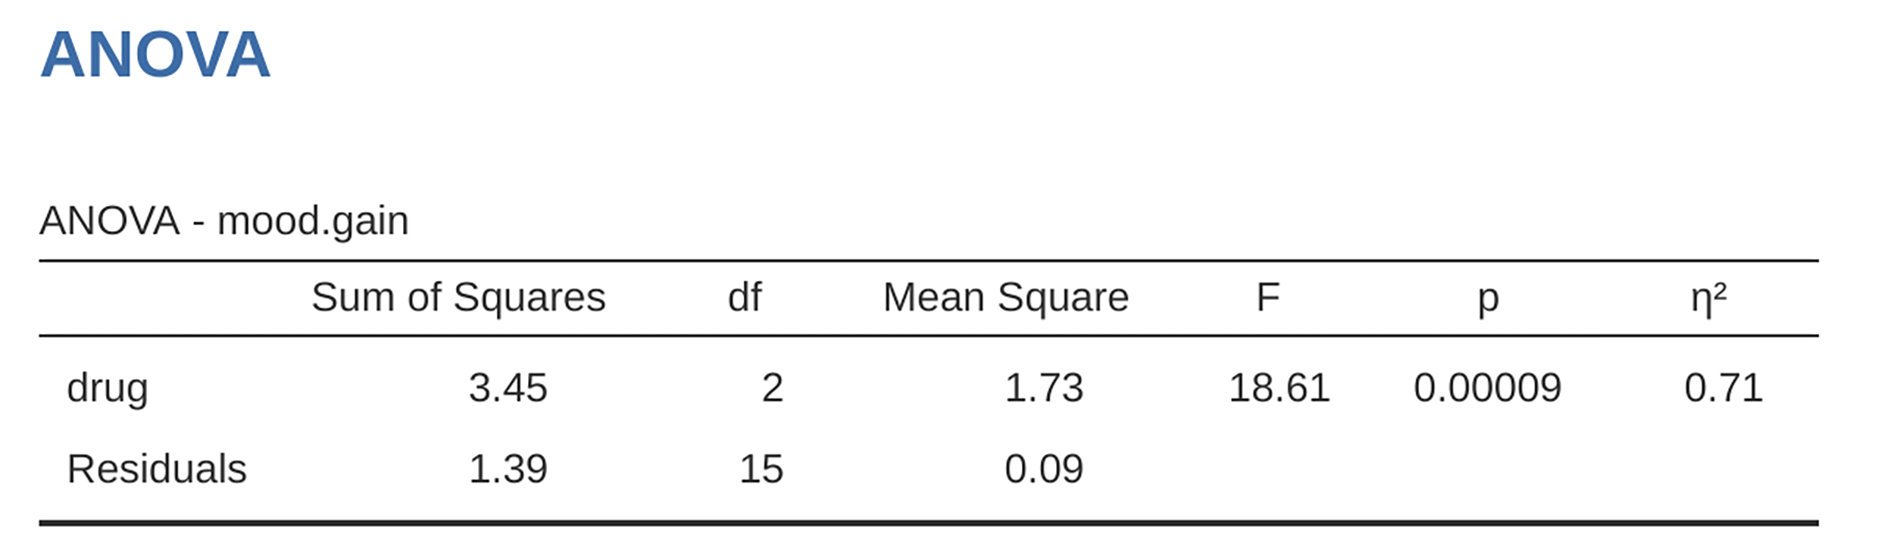
\includegraphics[width=1\textwidth,height=\textheight]{images/fig13-3.png} \hfill{}

\caption{\label{fig-fig13-3}jamovi results table for ANOVA of mood gain
by drug administered}

\end{figure}

The jamovi results table shows you the sums of squares values, the
degrees of freedom, and a couple of other quantities that we're not
really interested in right now. Notice, however, that jamovi doesn't use
the names ``between group'' and ``within group''. Instead, it tries to
assign more meaningful names. In our particular example, the between
groups variance corresponds to the effect that the drug has on the
outcome variable, and the within groups variance corresponds to the
``leftover'' variability so it calls that the residuals. If we compare
these numbers to the numbers that I calculated by hand in
\protect\hyperlink{a-worked-example}{A worked example}, you can see that
they're more or less the same, apart from rounding errors. The between
groups sums of squares is \(SS_b = 3.45\), the within groups sums of
squares is \(SS_w = 1.39\), and the degrees of freedom are \(2\) and
\(15\) respectively. We also get the \(F\)-value and the \(p\)-value
and, again, these are more or less the same, give or take rounding
errors, to the numbers that we calculated ourselves when doing it the
long and tedious way.

\hypertarget{effect-size}{%
\section{Effect size}\label{effect-size}}

There's a few different ways you could measure the effect size in an
ANOVA, but the most commonly used measures are \(\eta^2\) (eta squared)
and partial \(\eta^2\). For a one-way analysis of variance they're
identical to each other, so for the moment I'll just explain \(\eta^2\).
The definition of \(\eta^2\) is actually really simple:

\[\eta^2=\frac{SS_b}{SS_{tot}}\]

That's all it is. So when I look at the ANOVA table in
Figure~\ref{fig-fig13-3}, I see that \(SS_b = 3.45\) and
\(SS_tot = 3.45 + 1.39 = 4.84\). Thus we get an \(\eta^2\) value of:

\[\eta^2=\frac{3.45}{4.84}=0.71\]

The interpretation of \(\eta^2\) is equally straightforward. It refers
to the proportion of the variability in the outcome variable (mood.gain)
that can be explained in terms of the predictor (drug). A value of
\(\eta^2=0\) means that there is no relationship at all between the two,
whereas a value of \(\eta^2=1\) means that the relationship is perfect.
Better yet, the \(\eta^2\) value is very closely related to \(R^2\), as
discussed previously in Section~\ref{sec-The-R2-value}, and has an
equivalent interpretation. Although many statistics textbooks suggest
\(\eta^2\) as the default effect size measure in ANOVA, there's an
interesting blog post by Daniel Lakens suggesting that eta-squared is
perhaps not the best measure of effect size in real-world data analysis,
because it can be a biased estimator. Usefully, there is also an option
in jamovi to specify omega-squared (\(\omega^2\)), which is less biased,
alongside eta-squared.

\hypertarget{multiple-comparisons-and-post-hoc-tests}{%
\section{Multiple comparisons and post hoc
tests}\label{multiple-comparisons-and-post-hoc-tests}}

Any time you run an ANOVA with more than two groups and you end up with
a significant effect, the first thing you'll probably want to ask is
which groups are actually different from one another. In our drugs
example, our null hypothesis was that all three drugs (placebo, Anxifree
and Joyzepam) have the exact same effect on mood. But if you think about
it, the null hypothesis is actually claiming three different things all
at once here. Specifically, it claims that:

\begin{itemize}
\tightlist
\item
  Your competitor's drug (Anxifree) is no better than a placebo (i.e.,
  \(\mu_A = \mu_P\) )
\item
  Your drug (Joyzepam) is no better than a placebo (i.e.,
  \(\mu_J = \mu_P\) )
\item
  Anxifree and Joyzepam are equally effective (i.e., \(\mu_J = \mu_A\))
\end{itemize}

If any one of those three claims is false, then the null hypothesis is
also false. So, now that we've rejected our null hypothesis, we're
thinking that at least one of those things isn't true. But which ones?
All three of these propositions are of interest. Since you certainly
want to know if your new drug Joyzepam is better than a placebo, it
would be nice to know how well it stacks up against an existing
commercial alternative (i.e., Anxifree). It would even be useful to
check the performance of Anxifree against the placebo. Even if Anxifree
has already been extensively tested against placebos by other
researchers, it can still be very useful to check that your study is
producing similar results to earlier work.

When we characterise the null hypothesis in terms of these three
distinct propositions, it becomes clear that there are eight possible
``states of the world'' that we need to distinguish between
(Table~\ref{tbl-tab13-9}).

\hypertarget{tbl-tab13-9}{}
 
  \providecommand{\huxb}[2]{\arrayrulecolor[RGB]{#1}\global\arrayrulewidth=#2pt}
  \providecommand{\huxvb}[2]{\color[RGB]{#1}\vrule width #2pt}
  \providecommand{\huxtpad}[1]{\rule{0pt}{#1}}
  \providecommand{\huxbpad}[1]{\rule[-#1]{0pt}{#1}}

\begin{table}[ht]
\caption{\label{tbl-tab13-9}The null hypothesis and eight possible ``states of the world'' }\tabularnewline

\begin{centerbox}
\begin{threeparttable}
\setlength{\tabcolsep}{0pt}
\begin{tabularx}{0.9\textwidth}{p{0.18\textwidth} p{0.18\textwidth} p{0.18\textwidth} p{0.18\textwidth} p{0.18\textwidth}}


\hhline{>{\huxb{0, 0, 0}{0.4}}->{\huxb{0, 0, 0}{0.4}}->{\huxb{0, 0, 0}{0.4}}->{\huxb{0, 0, 0}{0.4}}->{\huxb{0, 0, 0}{0.4}}-}
\arrayrulecolor{black}

\multicolumn{1}{!{\huxvb{0, 0, 0}{0}}p{0.18\textwidth}!{\huxvb{0, 0, 0}{0}}}{\hspace{0pt}\parbox[b]{0.18\textwidth-0pt-12pt}{\huxtpad{2pt + 1em}\centering \textbf{possibility:}\huxbpad{2pt}}} &
\multicolumn{1}{p{0.18\textwidth}!{\huxvb{0, 0, 0}{0}}}{\hspace{12pt}\parbox[b]{0.18\textwidth-12pt-12pt}{\huxtpad{2pt + 1em}\centering \textbf{is \( \mu_P = \mu_A \)?}\huxbpad{2pt}}} &
\multicolumn{1}{p{0.18\textwidth}!{\huxvb{0, 0, 0}{0}}}{\hspace{12pt}\parbox[b]{0.18\textwidth-12pt-12pt}{\huxtpad{2pt + 1em}\centering \textbf{is \( \mu_P = \mu_J \)?}\huxbpad{2pt}}} &
\multicolumn{1}{p{0.18\textwidth}!{\huxvb{0, 0, 0}{0}}}{\hspace{12pt}\parbox[b]{0.18\textwidth-12pt-12pt}{\huxtpad{2pt + 1em}\centering \textbf{is \( \mu_A = \mu_J \)?}\huxbpad{2pt}}} &
\multicolumn{1}{p{0.18\textwidth}!{\huxvb{0, 0, 0}{0}}}{\hspace{12pt}\parbox[b]{0.18\textwidth-12pt-0pt}{\huxtpad{2pt + 1em}\centering \textbf{which hypothesis?}\huxbpad{2pt}}} \tabularnewline[-0.5pt]


\hhline{>{\huxb{0, 0, 0}{0.4}}->{\huxb{0, 0, 0}{0.4}}->{\huxb{0, 0, 0}{0.4}}->{\huxb{0, 0, 0}{0.4}}->{\huxb{0, 0, 0}{0.4}}-}
\arrayrulecolor{black}

\multicolumn{1}{!{\huxvb{0, 0, 0}{0}}p{0.18\textwidth}!{\huxvb{0, 0, 0}{0}}}{\hspace{0pt}\parbox[b]{0.18\textwidth-0pt-12pt}{\huxtpad{2pt + 1em}\centering 1\huxbpad{2pt}}} &
\multicolumn{1}{p{0.18\textwidth}!{\huxvb{0, 0, 0}{0}}}{\hspace{12pt}\parbox[b]{0.18\textwidth-12pt-12pt}{\huxtpad{2pt + 1em}\centering \( \checkmark \)\huxbpad{2pt}}} &
\multicolumn{1}{p{0.18\textwidth}!{\huxvb{0, 0, 0}{0}}}{\hspace{12pt}\parbox[b]{0.18\textwidth-12pt-12pt}{\huxtpad{2pt + 1em}\centering \( \checkmark \)\huxbpad{2pt}}} &
\multicolumn{1}{p{0.18\textwidth}!{\huxvb{0, 0, 0}{0}}}{\hspace{12pt}\parbox[b]{0.18\textwidth-12pt-12pt}{\huxtpad{2pt + 1em}\centering \( \checkmark \)\huxbpad{2pt}}} &
\multicolumn{1}{p{0.18\textwidth}!{\huxvb{0, 0, 0}{0}}}{\hspace{12pt}\parbox[b]{0.18\textwidth-12pt-0pt}{\huxtpad{2pt + 1em}\centering null\huxbpad{2pt}}} \tabularnewline[-0.5pt]


\hhline{}
\arrayrulecolor{black}

\multicolumn{1}{!{\huxvb{0, 0, 0}{0}}p{0.18\textwidth}!{\huxvb{0, 0, 0}{0}}}{\hspace{0pt}\parbox[b]{0.18\textwidth-0pt-12pt}{\huxtpad{2pt + 1em}\centering 2\huxbpad{2pt}}} &
\multicolumn{1}{p{0.18\textwidth}!{\huxvb{0, 0, 0}{0}}}{\hspace{12pt}\parbox[b]{0.18\textwidth-12pt-12pt}{\huxtpad{2pt + 1em}\centering \( \checkmark \)\huxbpad{2pt}}} &
\multicolumn{1}{p{0.18\textwidth}!{\huxvb{0, 0, 0}{0}}}{\hspace{12pt}\parbox[b]{0.18\textwidth-12pt-12pt}{\huxtpad{2pt + 1em}\centering \( \checkmark \)\huxbpad{2pt}}} &
\multicolumn{1}{p{0.18\textwidth}!{\huxvb{0, 0, 0}{0}}}{\hspace{12pt}\parbox[b]{0.18\textwidth-12pt-12pt}{\huxtpad{2pt + 1em}\centering \huxbpad{2pt}}} &
\multicolumn{1}{p{0.18\textwidth}!{\huxvb{0, 0, 0}{0}}}{\hspace{12pt}\parbox[b]{0.18\textwidth-12pt-0pt}{\huxtpad{2pt + 1em}\centering alternative\huxbpad{2pt}}} \tabularnewline[-0.5pt]


\hhline{}
\arrayrulecolor{black}

\multicolumn{1}{!{\huxvb{0, 0, 0}{0}}p{0.18\textwidth}!{\huxvb{0, 0, 0}{0}}}{\hspace{0pt}\parbox[b]{0.18\textwidth-0pt-12pt}{\huxtpad{2pt + 1em}\centering 3\huxbpad{2pt}}} &
\multicolumn{1}{p{0.18\textwidth}!{\huxvb{0, 0, 0}{0}}}{\hspace{12pt}\parbox[b]{0.18\textwidth-12pt-12pt}{\huxtpad{2pt + 1em}\centering \( \checkmark \)\huxbpad{2pt}}} &
\multicolumn{1}{p{0.18\textwidth}!{\huxvb{0, 0, 0}{0}}}{\hspace{12pt}\parbox[b]{0.18\textwidth-12pt-12pt}{\huxtpad{2pt + 1em}\centering \huxbpad{2pt}}} &
\multicolumn{1}{p{0.18\textwidth}!{\huxvb{0, 0, 0}{0}}}{\hspace{12pt}\parbox[b]{0.18\textwidth-12pt-12pt}{\huxtpad{2pt + 1em}\centering \( \checkmark \)\huxbpad{2pt}}} &
\multicolumn{1}{p{0.18\textwidth}!{\huxvb{0, 0, 0}{0}}}{\hspace{12pt}\parbox[b]{0.18\textwidth-12pt-0pt}{\huxtpad{2pt + 1em}\centering alternative\huxbpad{2pt}}} \tabularnewline[-0.5pt]


\hhline{}
\arrayrulecolor{black}

\multicolumn{1}{!{\huxvb{0, 0, 0}{0}}p{0.18\textwidth}!{\huxvb{0, 0, 0}{0}}}{\hspace{0pt}\parbox[b]{0.18\textwidth-0pt-12pt}{\huxtpad{2pt + 1em}\centering 4\huxbpad{2pt}}} &
\multicolumn{1}{p{0.18\textwidth}!{\huxvb{0, 0, 0}{0}}}{\hspace{12pt}\parbox[b]{0.18\textwidth-12pt-12pt}{\huxtpad{2pt + 1em}\centering \( \checkmark \)\huxbpad{2pt}}} &
\multicolumn{1}{p{0.18\textwidth}!{\huxvb{0, 0, 0}{0}}}{\hspace{12pt}\parbox[b]{0.18\textwidth-12pt-12pt}{\huxtpad{2pt + 1em}\centering \huxbpad{2pt}}} &
\multicolumn{1}{p{0.18\textwidth}!{\huxvb{0, 0, 0}{0}}}{\hspace{12pt}\parbox[b]{0.18\textwidth-12pt-12pt}{\huxtpad{2pt + 1em}\centering \huxbpad{2pt}}} &
\multicolumn{1}{p{0.18\textwidth}!{\huxvb{0, 0, 0}{0}}}{\hspace{12pt}\parbox[b]{0.18\textwidth-12pt-0pt}{\huxtpad{2pt + 1em}\centering alternative\huxbpad{2pt}}} \tabularnewline[-0.5pt]


\hhline{}
\arrayrulecolor{black}

\multicolumn{1}{!{\huxvb{0, 0, 0}{0}}p{0.18\textwidth}!{\huxvb{0, 0, 0}{0}}}{\hspace{0pt}\parbox[b]{0.18\textwidth-0pt-12pt}{\huxtpad{2pt + 1em}\centering 5\huxbpad{2pt}}} &
\multicolumn{1}{p{0.18\textwidth}!{\huxvb{0, 0, 0}{0}}}{\hspace{12pt}\parbox[b]{0.18\textwidth-12pt-12pt}{\huxtpad{2pt + 1em}\centering \( \checkmark \)\huxbpad{2pt}}} &
\multicolumn{1}{p{0.18\textwidth}!{\huxvb{0, 0, 0}{0}}}{\hspace{12pt}\parbox[b]{0.18\textwidth-12pt-12pt}{\huxtpad{2pt + 1em}\centering \( \checkmark \)\huxbpad{2pt}}} &
\multicolumn{1}{p{0.18\textwidth}!{\huxvb{0, 0, 0}{0}}}{\hspace{12pt}\parbox[b]{0.18\textwidth-12pt-12pt}{\huxtpad{2pt + 1em}\centering \( \checkmark \)\huxbpad{2pt}}} &
\multicolumn{1}{p{0.18\textwidth}!{\huxvb{0, 0, 0}{0}}}{\hspace{12pt}\parbox[b]{0.18\textwidth-12pt-0pt}{\huxtpad{2pt + 1em}\centering alternative\huxbpad{2pt}}} \tabularnewline[-0.5pt]


\hhline{}
\arrayrulecolor{black}

\multicolumn{1}{!{\huxvb{0, 0, 0}{0}}p{0.18\textwidth}!{\huxvb{0, 0, 0}{0}}}{\hspace{0pt}\parbox[b]{0.18\textwidth-0pt-12pt}{\huxtpad{2pt + 1em}\centering 6\huxbpad{2pt}}} &
\multicolumn{1}{p{0.18\textwidth}!{\huxvb{0, 0, 0}{0}}}{\hspace{12pt}\parbox[b]{0.18\textwidth-12pt-12pt}{\huxtpad{2pt + 1em}\centering \huxbpad{2pt}}} &
\multicolumn{1}{p{0.18\textwidth}!{\huxvb{0, 0, 0}{0}}}{\hspace{12pt}\parbox[b]{0.18\textwidth-12pt-12pt}{\huxtpad{2pt + 1em}\centering \( \checkmark \)\huxbpad{2pt}}} &
\multicolumn{1}{p{0.18\textwidth}!{\huxvb{0, 0, 0}{0}}}{\hspace{12pt}\parbox[b]{0.18\textwidth-12pt-12pt}{\huxtpad{2pt + 1em}\centering \huxbpad{2pt}}} &
\multicolumn{1}{p{0.18\textwidth}!{\huxvb{0, 0, 0}{0}}}{\hspace{12pt}\parbox[b]{0.18\textwidth-12pt-0pt}{\huxtpad{2pt + 1em}\centering alternative\huxbpad{2pt}}} \tabularnewline[-0.5pt]


\hhline{}
\arrayrulecolor{black}

\multicolumn{1}{!{\huxvb{0, 0, 0}{0}}p{0.18\textwidth}!{\huxvb{0, 0, 0}{0}}}{\hspace{0pt}\parbox[b]{0.18\textwidth-0pt-12pt}{\huxtpad{2pt + 1em}\centering 7\huxbpad{2pt}}} &
\multicolumn{1}{p{0.18\textwidth}!{\huxvb{0, 0, 0}{0}}}{\hspace{12pt}\parbox[b]{0.18\textwidth-12pt-12pt}{\huxtpad{2pt + 1em}\centering \huxbpad{2pt}}} &
\multicolumn{1}{p{0.18\textwidth}!{\huxvb{0, 0, 0}{0}}}{\hspace{12pt}\parbox[b]{0.18\textwidth-12pt-12pt}{\huxtpad{2pt + 1em}\centering \huxbpad{2pt}}} &
\multicolumn{1}{p{0.18\textwidth}!{\huxvb{0, 0, 0}{0}}}{\hspace{12pt}\parbox[b]{0.18\textwidth-12pt-12pt}{\huxtpad{2pt + 1em}\centering \( \checkmark \)\huxbpad{2pt}}} &
\multicolumn{1}{p{0.18\textwidth}!{\huxvb{0, 0, 0}{0}}}{\hspace{12pt}\parbox[b]{0.18\textwidth-12pt-0pt}{\huxtpad{2pt + 1em}\centering alternative\huxbpad{2pt}}} \tabularnewline[-0.5pt]


\hhline{}
\arrayrulecolor{black}

\multicolumn{1}{!{\huxvb{0, 0, 0}{0}}p{0.18\textwidth}!{\huxvb{0, 0, 0}{0}}}{\hspace{0pt}\parbox[b]{0.18\textwidth-0pt-12pt}{\huxtpad{2pt + 1em}\centering 8\huxbpad{2pt}}} &
\multicolumn{1}{p{0.18\textwidth}!{\huxvb{0, 0, 0}{0}}}{\hspace{12pt}\parbox[b]{0.18\textwidth-12pt-12pt}{\huxtpad{2pt + 1em}\centering \huxbpad{2pt}}} &
\multicolumn{1}{p{0.18\textwidth}!{\huxvb{0, 0, 0}{0}}}{\hspace{12pt}\parbox[b]{0.18\textwidth-12pt-12pt}{\huxtpad{2pt + 1em}\centering \huxbpad{2pt}}} &
\multicolumn{1}{p{0.18\textwidth}!{\huxvb{0, 0, 0}{0}}}{\hspace{12pt}\parbox[b]{0.18\textwidth-12pt-12pt}{\huxtpad{2pt + 1em}\centering \huxbpad{2pt}}} &
\multicolumn{1}{p{0.18\textwidth}!{\huxvb{0, 0, 0}{0}}}{\hspace{12pt}\parbox[b]{0.18\textwidth-12pt-0pt}{\huxtpad{2pt + 1em}\centering alternative\huxbpad{2pt}}} \tabularnewline[-0.5pt]


\hhline{>{\huxb{0, 0, 0}{0.4}}->{\huxb{0, 0, 0}{0.4}}->{\huxb{0, 0, 0}{0.4}}->{\huxb{0, 0, 0}{0.4}}->{\huxb{0, 0, 0}{0.4}}-}
\arrayrulecolor{black}
\end{tabularx} 

\end{threeparttable}\par\end{centerbox}

\end{table}
 

By rejecting the null hypothesis, we've decided that we don't believe
that \#1 is the true state of the world. The next question to ask is,
which of the other seven possibilities \emph{do} we think is right? When
faced with this situation, it's usually helps to look at the data. For
instance, if we look at the plots in Figure~\ref{fig-fig13-1}, it's
tempting to conclude that Joyzepam is better than the placebo and better
than Anxifree, but there's no real difference between Anxifree and the
placebo. However, if we want to get a clearer answer about this, it
might help to run some tests.

\hypertarget{running-pairwise-t-tests}{%
\subsection{\texorpdfstring{Running ``pairwise''
\(t\)-tests}{Running ``pairwise'' t-tests}}\label{running-pairwise-t-tests}}

How might we go about solving our problem? Given that we've got three
separate pairs of means (placebo versus Anxifree, placebo versus
Joyzepam, and Anxifree versus Joyzepam) to compare, what we could do is
run three separate \(t\)-tests and see what happens. This is easy to do
in jamovi. Go to the ANOVA `Post Hoc Tests' options, move the `drug'
variable across into the active box on the right, and then click on the
`No correction' checkbox. This will produce a neat table showing all the
pairwise \(t\)-test comparisons amongst the three levels of the drug
variable, as in Figure~\ref{fig-fig13-4}.

\begin{figure}

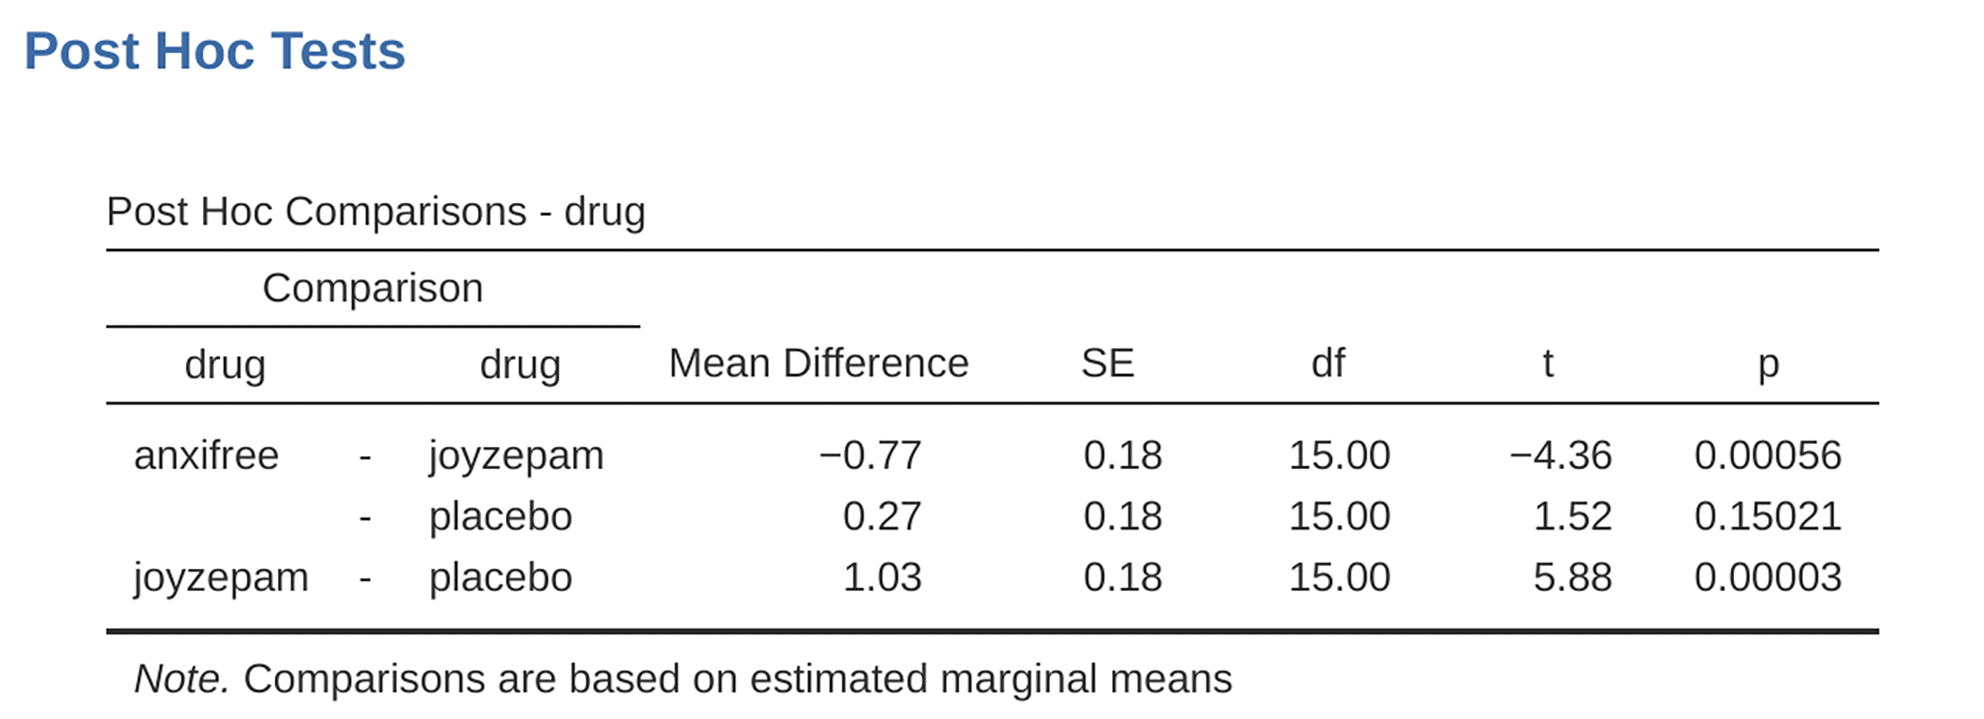
\includegraphics[width=1\textwidth,height=\textheight]{images/fig13-4.png} \hfill{}

\caption{\label{fig-fig13-4}Uncorrected pairwise \(t\)-tests as post hoc
comparisons in jamovi}

\end{figure}

\hypertarget{corrections-for-multiple-testing}{%
\subsection{Corrections for multiple
testing}\label{corrections-for-multiple-testing}}

In the previous section I hinted that there's a problem with just
running lots and lots of \(t\)-tests. The concern is that, when running
these analyses, what we're doing is going on a ``fishing expedition''.
We're running lots and lots of tests without much theoretical guidance
in the hope that some of them come up significant. This kind of
theory-free search for group differences is referred to as \textbf{post
hoc analysis} (``post hoc'' being Latin for ``after this'').\footnote{If
  you \emph{do} have some theoretical basis for wanting to investigate
  some comparisons but not others, it's a different story. In those
  circumstances you're not really running ``post hoc'' analyses at all,
  you're making ``planned comparisons''. I do talk about this situation
  later in the book -
  Section~\ref{sec-The-method-of-planned-comparisons}, but for now I
  want to keep things simple.}

It's okay to run post hoc analyses, but a lot of care is required. For
instance, the analysis that I ran in the previous section should be
avoided, as each individual \(t\)-test is designed to have a 5\% type I
error rate (i.e., \(\alpha = .05\)) and I ran three of these tests.
Imagine what would have happened if my ANOVA involved 10 different
groups, and I had decided to run 45 ``post hoc'' \(t\)-tests to try to
find out which ones were significantly different from each other, you'd
expect 2 or 3 of them to come up significant by chance alone. As we saw
in \textbf{?@sec-Hypothesis-testing}, the central organising principle
behind null hypothesis testing is that we seek to control our type I
error rate, but now that I'm running lots of \(t\)-tests at once in
order to determine the source of my ANOVA results, my actual type I
error rate across this whole family of tests has gotten completely out
of control.

The usual solution to this problem is to introduce an adjustment to the
\(p\)-value, which aims to control the total error rate across the
family of tests (see Shaffer (1995)). An adjustment of this form, which
is usually (but not always) applied because one is doing post hoc
analysis, is often referred to as a \textbf{correction for multiple
comparisons}, though it is sometimes referred to as ``simultaneous
inference''. In any case, there are quite a few different ways of doing
this adjustment. I'll discuss a few of them in this section and in
Section~\ref{sec-Post-hoc-tests} in the next chapter, but you should be
aware that there are many other methods out there (see, e.g., Hsu
(1996)).

\hypertarget{bonferroni-corrections}{%
\subsection{Bonferroni corrections}\label{bonferroni-corrections}}

The simplest of these adjustments is called the \textbf{Bonferroni
correction} (Dunn, 1961), and it's very very simple indeed. Suppose that
my post hoc analysis consists of \(m\) separate tests, and I want to
ensure that the total probability of making \emph{any} type I errors at
all is at most \(\alpha\).\footnote{It's worth noting in passing that
  not all adjustment methods try to do this. What I've described here is
  an approach for controlling ``family wise type I error rate''.
  However, there are other post hoc tests that seek to control the
  ``false discovery rate'', which is a somewhat different thing.} If so,
then the Bonferroni correction just says ``multiply all your raw
\(p\)-values by \(m\)''. If we let \(p\) denote the original
\(p\)-value, and let \(p_j^{'}\) be the corrected value, then the
Bonferroni correction tells that:

\[p_j^{'}=m \times p\] And therefore, if you're using the Bonferroni
correction, you would reject the null hypothesis if
\(p_j^{'} < \alpha\). The logic behind this correction is very
straightforward. We're doing m different tests, so if we arrange it so
that each test has a type I error rate of at most \(\frac{\alpha}{m}\),
then the \emph{total} type I error rate across these tests cannot be
larger than \(\alpha\). That's pretty simple, so much so that in the
original paper, the author writes:

\begin{quote}
The method given here is so simple and so general that I am sure it must
have been used before this. I do not find it, however, so can only
conclude that perhaps its very simplicity has kept statisticians from
realizing that it is a very good method in some situations (Dunn (1961),
pp.~52-53).
\end{quote}

To use the Bonferroni correction in jamovi, just click on the
`Bonferroni' checkbox in the `Correction' options, and you will see
another column added to the ANOVA results table showing the adjusted
\(p\)-values for the Bonferroni correction (Table~\ref{tbl-tab13-8}). If
we compare these three \(p\)-values to those for the uncorrected,
pairwise \(t\)-tests, it is clear that the only thing that jamovi has
done is multiply them by \(3\).

\hypertarget{holm-corrections}{%
\subsection{Holm corrections}\label{holm-corrections}}

Although the Bonferroni correction is the simplest adjustment out there,
it's not usually the best one to use. One method that is often used
instead is the \textbf{Holm correction} (Holm, 1979). The idea behind
the Holm correction is to pretend that you're doing the tests
sequentially, starting with the smallest (raw) \(p\)-value and moving
onto the largest one. For the \(j\)-th largest of the \(p\)-values, the
adjustment is \emph{either}:

\[p_j^{'}=j \times p_j\]

(i.e., the biggest \(p\)-value remains unchanged, the second biggest
\(p\)-value is doubled, the third biggest \(p\)-value is tripled, and so
on), or:

\[p_j^{'}=p_{j+1}^{'}\]

whichever one is larger. This might sound a little confusing, so let's
go through it a little more slowly. Here's what the Holm correction
does. First, you sort all of your \(p\)-values in order, from smallest
to largest. For the smallest \(p\)-value all you do is multiply it by
\(m\), and you're done. However, for all the other ones it's a two-stage
process. For instance, when you move to the second smallest \(p\)-value,
you first multiply it by \(m - 1\). If this produces a number that is
bigger than the adjusted \(p\)-value that you got last time, then you
keep it. But if it's smaller than the last one, then you copy the last
\(p\)-value. To illustrate how this works, consider
Table~\ref{tbl-tab13-10} which shows the calculations of a Holm
correction for a collection of five \(p\)-values.

\hypertarget{tbl-tab13-10}{}
 
  \providecommand{\huxb}[2]{\arrayrulecolor[RGB]{#1}\global\arrayrulewidth=#2pt}
  \providecommand{\huxvb}[2]{\color[RGB]{#1}\vrule width #2pt}
  \providecommand{\huxtpad}[1]{\rule{0pt}{#1}}
  \providecommand{\huxbpad}[1]{\rule[-#1]{0pt}{#1}}

\begin{table}[ht]
\caption{\label{tbl-tab13-10}Holm corrected \(p\)-values }\tabularnewline

\begin{centerbox}
\begin{threeparttable}
\setlength{\tabcolsep}{0pt}
\begin{tabularx}{0.9\textwidth}{p{0.225\textwidth} p{0.225\textwidth} p{0.225\textwidth} p{0.225\textwidth}}


\hhline{>{\huxb{0, 0, 0}{0.4}}->{\huxb{0, 0, 0}{0.4}}->{\huxb{0, 0, 0}{0.4}}->{\huxb{0, 0, 0}{0.4}}-}
\arrayrulecolor{black}

\multicolumn{1}{!{\huxvb{0, 0, 0}{0}}p{0.225\textwidth}!{\huxvb{0, 0, 0}{0}}}{\hspace{0pt}\parbox[b]{0.225\textwidth-0pt-12pt}{\huxtpad{2pt + 1em}\centering \textbf{raw \( p \)}\huxbpad{2pt}}} &
\multicolumn{1}{p{0.225\textwidth}!{\huxvb{0, 0, 0}{0}}}{\hspace{12pt}\parbox[b]{0.225\textwidth-12pt-12pt}{\huxtpad{2pt + 1em}\centering \textbf{rank \( j \)}\huxbpad{2pt}}} &
\multicolumn{1}{p{0.225\textwidth}!{\huxvb{0, 0, 0}{0}}}{\hspace{12pt}\parbox[b]{0.225\textwidth-12pt-12pt}{\huxtpad{2pt + 1em}\centering \textbf{\( p \times j \)}\huxbpad{2pt}}} &
\multicolumn{1}{p{0.225\textwidth}!{\huxvb{0, 0, 0}{0}}}{\hspace{12pt}\parbox[b]{0.225\textwidth-12pt-0pt}{\huxtpad{2pt + 1em}\centering \textbf{Holm \( p \)}\huxbpad{2pt}}} \tabularnewline[-0.5pt]


\hhline{>{\huxb{0, 0, 0}{0.4}}->{\huxb{0, 0, 0}{0.4}}->{\huxb{0, 0, 0}{0.4}}->{\huxb{0, 0, 0}{0.4}}-}
\arrayrulecolor{black}

\multicolumn{1}{!{\huxvb{0, 0, 0}{0}}p{0.225\textwidth}!{\huxvb{0, 0, 0}{0}}}{\hspace{0pt}\parbox[b]{0.225\textwidth-0pt-12pt}{\huxtpad{2pt + 1em}\centering .001\huxbpad{2pt}}} &
\multicolumn{1}{p{0.225\textwidth}!{\huxvb{0, 0, 0}{0}}}{\hspace{12pt}\parbox[b]{0.225\textwidth-12pt-12pt}{\huxtpad{2pt + 1em}\centering 5\huxbpad{2pt}}} &
\multicolumn{1}{p{0.225\textwidth}!{\huxvb{0, 0, 0}{0}}}{\hspace{12pt}\parbox[b]{0.225\textwidth-12pt-12pt}{\huxtpad{2pt + 1em}\centering .005\huxbpad{2pt}}} &
\multicolumn{1}{p{0.225\textwidth}!{\huxvb{0, 0, 0}{0}}}{\hspace{12pt}\parbox[b]{0.225\textwidth-12pt-0pt}{\huxtpad{2pt + 1em}\centering .005\huxbpad{2pt}}} \tabularnewline[-0.5pt]


\hhline{}
\arrayrulecolor{black}

\multicolumn{1}{!{\huxvb{0, 0, 0}{0}}p{0.225\textwidth}!{\huxvb{0, 0, 0}{0}}}{\hspace{0pt}\parbox[b]{0.225\textwidth-0pt-12pt}{\huxtpad{2pt + 1em}\centering .005\huxbpad{2pt}}} &
\multicolumn{1}{p{0.225\textwidth}!{\huxvb{0, 0, 0}{0}}}{\hspace{12pt}\parbox[b]{0.225\textwidth-12pt-12pt}{\huxtpad{2pt + 1em}\centering 4\huxbpad{2pt}}} &
\multicolumn{1}{p{0.225\textwidth}!{\huxvb{0, 0, 0}{0}}}{\hspace{12pt}\parbox[b]{0.225\textwidth-12pt-12pt}{\huxtpad{2pt + 1em}\centering .020\huxbpad{2pt}}} &
\multicolumn{1}{p{0.225\textwidth}!{\huxvb{0, 0, 0}{0}}}{\hspace{12pt}\parbox[b]{0.225\textwidth-12pt-0pt}{\huxtpad{2pt + 1em}\centering .020\huxbpad{2pt}}} \tabularnewline[-0.5pt]


\hhline{}
\arrayrulecolor{black}

\multicolumn{1}{!{\huxvb{0, 0, 0}{0}}p{0.225\textwidth}!{\huxvb{0, 0, 0}{0}}}{\hspace{0pt}\parbox[b]{0.225\textwidth-0pt-12pt}{\huxtpad{2pt + 1em}\centering .019\huxbpad{2pt}}} &
\multicolumn{1}{p{0.225\textwidth}!{\huxvb{0, 0, 0}{0}}}{\hspace{12pt}\parbox[b]{0.225\textwidth-12pt-12pt}{\huxtpad{2pt + 1em}\centering 3\huxbpad{2pt}}} &
\multicolumn{1}{p{0.225\textwidth}!{\huxvb{0, 0, 0}{0}}}{\hspace{12pt}\parbox[b]{0.225\textwidth-12pt-12pt}{\huxtpad{2pt + 1em}\centering .057\huxbpad{2pt}}} &
\multicolumn{1}{p{0.225\textwidth}!{\huxvb{0, 0, 0}{0}}}{\hspace{12pt}\parbox[b]{0.225\textwidth-12pt-0pt}{\huxtpad{2pt + 1em}\centering .057\huxbpad{2pt}}} \tabularnewline[-0.5pt]


\hhline{}
\arrayrulecolor{black}

\multicolumn{1}{!{\huxvb{0, 0, 0}{0}}p{0.225\textwidth}!{\huxvb{0, 0, 0}{0}}}{\hspace{0pt}\parbox[b]{0.225\textwidth-0pt-12pt}{\huxtpad{2pt + 1em}\centering .022\huxbpad{2pt}}} &
\multicolumn{1}{p{0.225\textwidth}!{\huxvb{0, 0, 0}{0}}}{\hspace{12pt}\parbox[b]{0.225\textwidth-12pt-12pt}{\huxtpad{2pt + 1em}\centering 2\huxbpad{2pt}}} &
\multicolumn{1}{p{0.225\textwidth}!{\huxvb{0, 0, 0}{0}}}{\hspace{12pt}\parbox[b]{0.225\textwidth-12pt-12pt}{\huxtpad{2pt + 1em}\centering .044\huxbpad{2pt}}} &
\multicolumn{1}{p{0.225\textwidth}!{\huxvb{0, 0, 0}{0}}}{\hspace{12pt}\parbox[b]{0.225\textwidth-12pt-0pt}{\huxtpad{2pt + 1em}\centering .057\huxbpad{2pt}}} \tabularnewline[-0.5pt]


\hhline{}
\arrayrulecolor{black}

\multicolumn{1}{!{\huxvb{0, 0, 0}{0}}p{0.225\textwidth}!{\huxvb{0, 0, 0}{0}}}{\hspace{0pt}\parbox[b]{0.225\textwidth-0pt-12pt}{\huxtpad{2pt + 1em}\centering .103\huxbpad{2pt}}} &
\multicolumn{1}{p{0.225\textwidth}!{\huxvb{0, 0, 0}{0}}}{\hspace{12pt}\parbox[b]{0.225\textwidth-12pt-12pt}{\huxtpad{2pt + 1em}\centering 1\huxbpad{2pt}}} &
\multicolumn{1}{p{0.225\textwidth}!{\huxvb{0, 0, 0}{0}}}{\hspace{12pt}\parbox[b]{0.225\textwidth-12pt-12pt}{\huxtpad{2pt + 1em}\centering .103\huxbpad{2pt}}} &
\multicolumn{1}{p{0.225\textwidth}!{\huxvb{0, 0, 0}{0}}}{\hspace{12pt}\parbox[b]{0.225\textwidth-12pt-0pt}{\huxtpad{2pt + 1em}\centering .103\huxbpad{2pt}}} \tabularnewline[-0.5pt]


\hhline{>{\huxb{0, 0, 0}{0.4}}->{\huxb{0, 0, 0}{0.4}}->{\huxb{0, 0, 0}{0.4}}->{\huxb{0, 0, 0}{0.4}}-}
\arrayrulecolor{black}
\end{tabularx} 

\end{threeparttable}\par\end{centerbox}

\end{table}
 

Hopefully that makes things clear.

Although it's a little harder to calculate, the Holm correction has some
very nice properties. It's more powerful than Bonferroni (i.e., it has a
lower type II error rate) but, counter-intuitive as it might seem, it
has the same type I error rate. As a consequence, in practice there's
never any reason to use the simpler Bonferroni correction since it is
always outperformed by the slightly more elaborate Holm correction.
Because of this, the Holm correction should be your \emph{go to}
multiple comparison correction. Figure~\ref{fig-fig13-4} also shows the
Holm corrected \(p\)-values and, as you can see, the biggest \(p\)-value
(corresponding to the comparison between Anxifree and the placebo) is
unaltered. At a value of .15, it is exactly the same as the value we got
originally when we applied no correction at all. In contrast, the
smallest \(p\)-value (Joyzepam versus placebo) has been multiplied by
three.

\hypertarget{writing-up-the-post-hoc-test}{%
\subsection{Writing up the post hoc
test}\label{writing-up-the-post-hoc-test}}

Finally, having run the post hoc analysis to determine which groups are
significantly different to one another, you might write up the result
like this:

\begin{quote}
Post hoc tests (using the Holm correction to adjust \(p\)) indicated
that Joyzepam produced a significantly larger mood change than both
Anxifree (\(p = .001\)) and the placebo (\((p = 9.0 \times{10^{-5}}\)).
We found no evidence that Anxifree performed better than the placebo
(\(p = .15\)).
\end{quote}

Or, if you don't like the idea of reporting exact \(p\)-values, then
you'd change those numbers to \(p < .01\), \(p < .001\) and \(p > .05\)
respectively. Either way, the key thing is that you indicate that you
used Holm's correction to adjust the \(p\)-values. And of course, I'm
assuming that elsewhere in the write up you've included the relevant
descriptive statistics (i.e., the group means and standard deviations),
since these \(p\)-values on their own aren't terribly informative.

\hypertarget{the-assumptions-of-one-way-anova}{%
\section{The assumptions of one-way
ANOVA}\label{the-assumptions-of-one-way-anova}}

Like any statistical test, analysis of variance relies on some
assumptions about the data, specifically the residuals. There are three
key assumptions that you need to be aware of: normality, homogeneity of
variance and independence.

{[}Additional technical detail\footnote{If you remember back to
  \protect\hyperlink{a-worked-example}{A worked example}, which I hope
  you at least skimmed even if you didn't read the whole thing, I
  described the statistical models underpinning ANOVA in this way:
  \[H_0:Y_{ik}=\mu + \epsilon_{ik}\]
  \[H_1:Y_{ik}=\mu_k + \epsilon_{ik}\] In these equations \(\mu\) refers
  to a single grand population mean which is the same for all groups,
  and µk is the population mean for the k-th group. Up to this point
  we've been mostly interested in whether our data are best described in
  terms of a single grand mean (the null hypothesis) or in terms of
  different group-specific means (the alternative hypothesis). This
  makes sense, of course, as that's actually the important research
  question! However, all of our testing procedures have, implicitly,
  relied on a specific assumption about the residuals,
  \(\epsilon\_{ik}\), namely that
  \[\epsilon_{ik} \sim Normal(0,\sigma^2)\] None of the maths works
  properly without this bit. Or, to be precise, you can still do all the
  calculations and you'll end up with an \(F\) statistic, but you have
  no guarantee that this \(F\) statistic actually measures what you
  think it's measuring, and so any conclusions that you might draw on
  the basis of the \(F\)-test might be wrong.}{]}

So, how do we check whether the assumption about the residuals is
accurate? Well, as I indicated above, there are three distinct claims
buried in this one statement, and we'll consider them separately.

\begin{itemize}
\tightlist
\item
  \textbf{Homogeneity of variance}. Notice that we've only got the one
  value for the population standard deviation (i.e., \(\sigma\)), rather
  than allowing each group to have it's own value (i.e., \(\sigma_k\)).
  This is referred to as the homogeneity of variance (sometimes called
  homoscedasticity) assumption. ANOVA assumes that the population
  standard deviation is the same for all groups. We'll talk about this
  extensively in the
  \protect\hyperlink{sec-Checking-the-homogeneity-of-variance-assumption}{Checking
  the homogeneity of variance assumption} section.
\item
  \textbf{Normality}. The residuals are assumed to be normally
  distributed. As we saw in
  \textbf{?@sec-Checking-the-normality-of-a-sample}, we can assess this
  by looking at QQ plots (or running a Shapiro-Wilk test. I'll talk
  about this more in an ANOVA context in the
  \protect\hyperlink{sec-Checking-the-normality-assumption}{Checking the
  normality assumption} section.
\item
  \textbf{Independence}. The independence assumption is a little
  trickier. What it basically means is that, knowing one residual tells
  you nothing about any other residual. All of the \(\epsilon_{ik}\)
  values are assumed to have been generated without any ``regard for''
  or ``relationship to'' any of the other ones. There's not an obvious
  or simple way to test for this, but there are some situations that are
  clear violations of this. For instance, if you have a repeated
  measures design, where each participant in your study appears in more
  than one condition, then independence doesn't hold. There's a special
  relationship between some observations, namely those that correspond
  to the same person! When that happens, you need to use something like
  a \protect\hyperlink{repeated-measures-one-way-anova}{Repeated
  measures one-way ANOVA}.
\end{itemize}

\hypertarget{sec-Checking-the-homogeneity-of-variance-assumption}{%
\subsection{Checking the homogeneity of variance
assumption}\label{sec-Checking-the-homogeneity-of-variance-assumption}}

\begin{quote}
``\emph{To make the preliminary test on variances is rather like putting
to sea in a rowing boat to find out whether conditions are sufficiently
calm for an ocean liner to leave port!}''\\
-- George Box (Box, 1953)
\end{quote}

There's more than one way to skin a cat, as the saying goes, and more
than one way to test the homogeneity of variance assumption, too (though
for some reason no-one made a saying out of that). The most commonly
used test for this that I've seen in the literature is the Levene test
(Levene, 1960), and the closely related Brown-Forsythe test (Brown \&
Forsythe, 1974).

Regardless of whether you're doing the standard Levene test or the
Brown-Forsythe test, the test statistic, which is sometimes denoted
\(F\) but also sometimes written as \(W\), is calculated in exactly the
same way that the \(F\) statistic for the regular ANOVA is calculated,
just using a \(Z_{ik}\) rather than \(Y_{ik}\). With that in mind, we
can go on to look at how to run the test in jamovi.

{[}Additional technical detail\footnote{The Levene test is shockingly
  simple. Suppose we have our outcome variable \(Y_{ik}\). All we do is
  define a new variable, which I'll call \(Z_{ik}\), corresponding to
  the absolute deviation from the group mean
  \[Z_{ik}=Y_{ik}-\bar{Y}_{k}\] Okay, what good does this do us? Well,
  let's take a moment to think about what \(Z_{ik}\) actually is and
  what we're trying to test. The value of \(Z_{ik}\) is a measure of how
  the \(i\)-th observation in the \(k\)-th group deviates from its group
  mean. And our null hypothesis is that all groups have the same
  variance, i.e., the same overall deviations from the group means! So
  the null hypothesis in a Levene test is that the population means of
  \(Z\) are identical for all groups. Hmm. So what we need now is a
  statistical test of the null hypothesis that all group means are
  identical. Where have we seen that before? Oh right, that's what ANOVA
  is, and so all that the Levene test does is run an ANOVA on the new
  variable \(Z_{ik}\). What about the Brown-Forsythe test? Does that do
  anything particularly different? Nope. The only change from the Levene
  test is that it constructs the transformed variable \(Z\) in a
  slightly different way, using deviations from the group medians rather
  than deviations from the group means. That is, for the Brown-Forsythe
  test: \[Z_{ik}=Y_{ik}-median_k(Y)\] where \(median_k(Y)\) is the
  median for group \(k\).}{]}

\hypertarget{running-the-levene-test-in-jamovi}{%
\subsection{Running the Levene test in
jamovi}\label{running-the-levene-test-in-jamovi}}

Okay, so how do we run the Levene test? Simple really -- under the ANOVA
`Assumption Checks' option, just click on the `Homogeneity tests'
checkbox. If we look at the output, shown in Figure~\ref{fig-fig13-5},
we see that the test is non-significant (\(F_{2,15} = 1.45, p = .266\)),
so it looks like the homogeneity of variance assumption is fine.
However, looks can be deceptive! If your sample size is pretty big, then
the Levene test could show up a significant effect (i.e.~p \textless{}
.05) even when the homogeneity of variance assumption is not violated to
an extent which troubles the robustness of ANOVA. This was the point
George Box was making in the quote above. Similarly, if your sample size
is quite small, then the homogeneity of variance assumption might not be
satisfied and yet a Levene test could be non-significant (i.e.~p
\textgreater{} .05). What this means is that, alongside any statistical
test of the assumption being met, you should always plot the standard
deviation around the means for each group / category in the
analysis\ldots just to see if they look fairly similar (i.e.~homogeneity
of variance) or not.

\begin{figure}

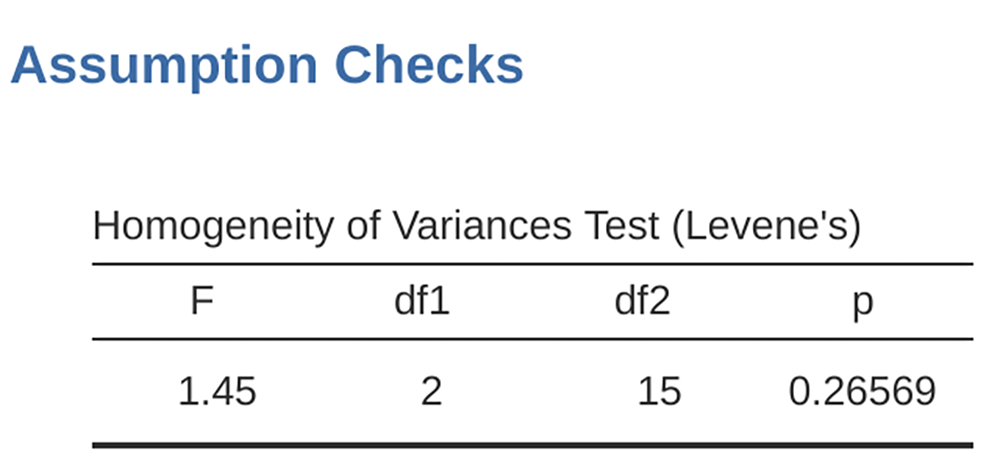
\includegraphics[width=1\textwidth,height=\textheight]{images/fig13-5.png} \hfill{}

\caption{\label{fig-fig13-5}Levene test output for one-way ANOVA in
jamovi}

\end{figure}

\hypertarget{removing-the-homogeneity-of-variance-assumption}{%
\subsection{Removing the homogeneity of variance
assumption}\label{removing-the-homogeneity-of-variance-assumption}}

In our example, the homogeneity of variance assumption turned out to be
a pretty safe one: the Levene test came back non-significant
(notwithstanding that we should also look at the plot of standard
deviations), so we probably don't need to worry. However, in real life
we aren't always that lucky. How do we save our ANOVA when the
homogeneity of variance assumption is violated? If you recall from our
discussion of \(t\)-tests, we've seen this problem before. The Student
\(t\)-test assumes equal variances, so the solution was to use the Welch
\(t\)-test, which does not. In fact, Welch (1951) also showed how we can
solve this problem for ANOVA too (the \textbf{Welch one-way test}). It's
implemented in jamovi using the One-Way ANOVA analysis. This is a
specific analysis approach just for one-way ANOVA, and to run the Welch
one-way ANOVA for our example, we would re-run the analysis as
previously, but this time use the jamovi ANOVA - one-way ANOVA analysis
command, and check the option for Welch's test (see
Figure~\ref{fig-fig13-6}). To understand what's happening here, let's
compare these numbers to what we got earlier when
\protect\hyperlink{running-an-anova-in-jamovi}{Running an ANOVA in
jamovi} originally. To save you the trouble of flicking back, this is
what we got last time: \(F(2, 15) = 18.611, p = .00009\), also shown as
the Fisher's test in the One-Way ANOVA shown in
Figure~\ref{fig-fig13-6}.

\begin{figure}

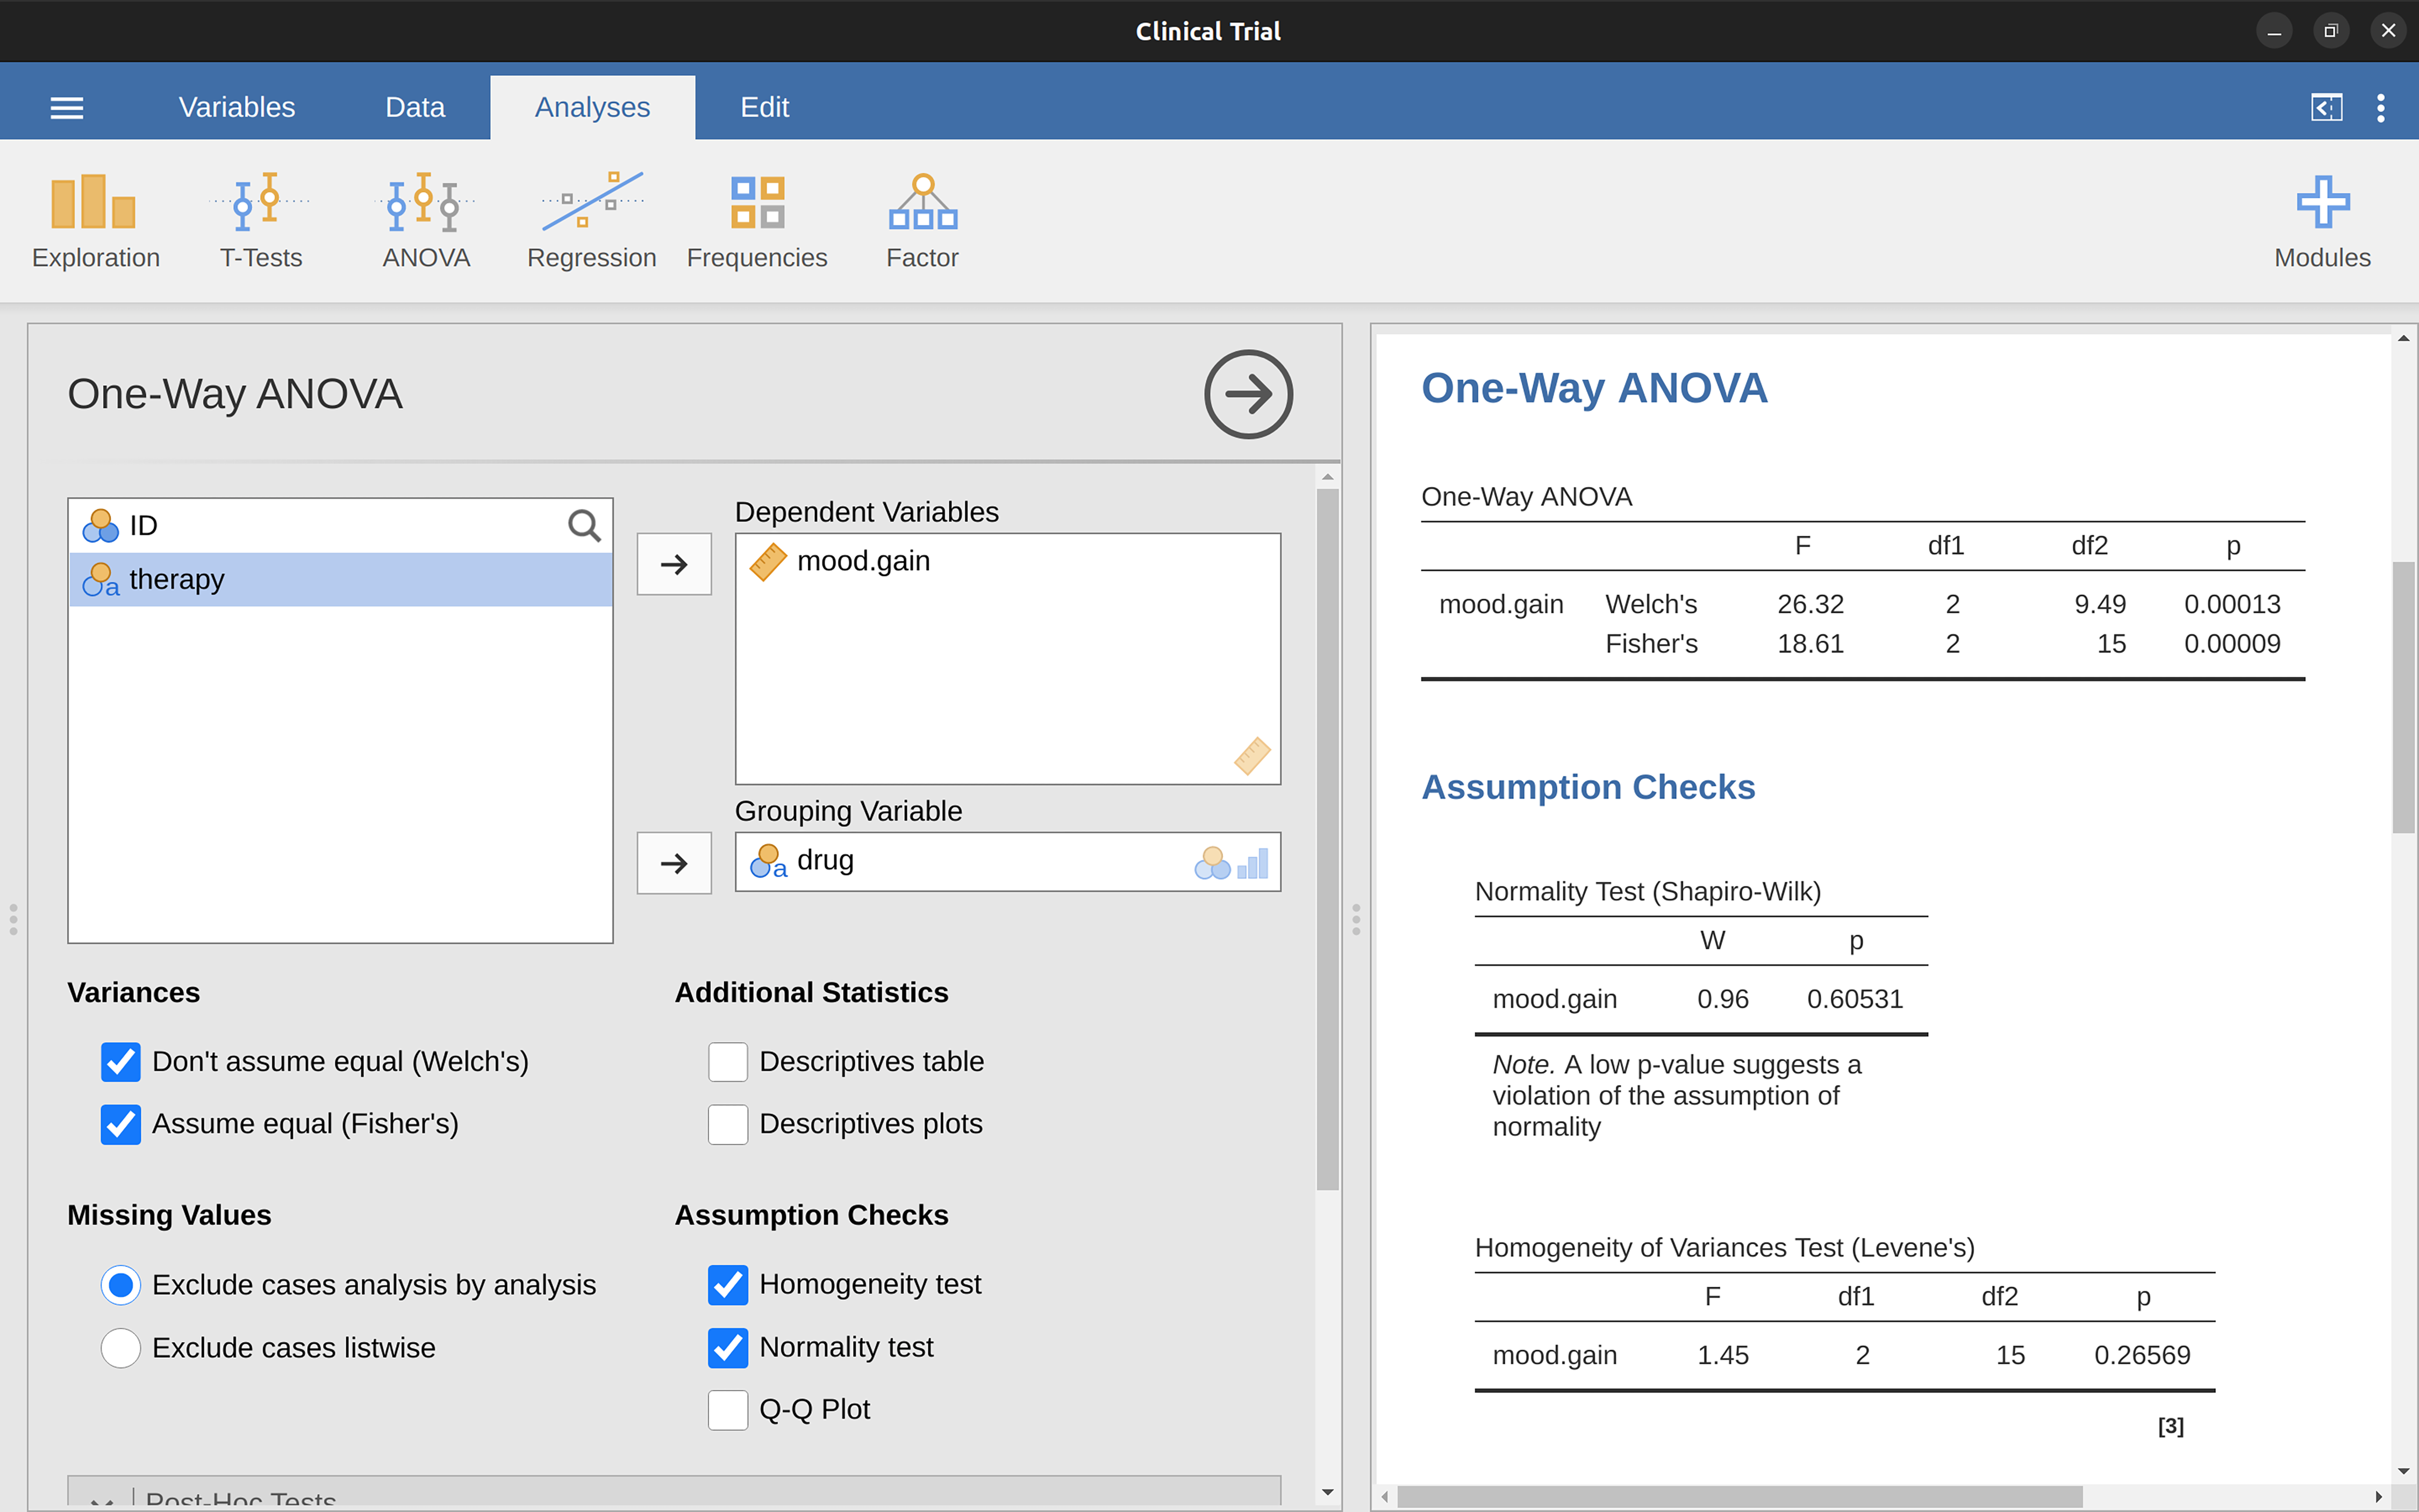
\includegraphics[width=1\textwidth,height=\textheight]{images/fig13-6.png} \hfill{}

\caption{\label{fig-fig13-6}Welch test as part of the one-way ANOVA
analysis in jamovi}

\end{figure}

Okay, so originally our ANOVA gave us the result \(F(2, 15) = 18.6\),
whereas the Welch one-way test gave us \(F(2, 9.49) = 26.32\). In other
words, the Welch test has reduced the within groups degrees of freedom
from 15 to 9.49, and the \(F\)-value has increased from 18.6 to 26.32.

\hypertarget{sec-Checking-the-normality-assumption}{%
\subsection{Checking the normality
assumption}\label{sec-Checking-the-normality-assumption}}

Testing the normality assumption is relatively straightforward. We
covered most of what you need to know in
\textbf{?@sec-Checking-the-normality-of-a-sample}. The only thing we
really need to do is draw a QQ plot and, in addition if it is available,
run the Shapiro-Wilk test. The QQ plot is shown in
Figure~\ref{fig-fig13-7} and it looks pretty normal to me. If the
Shapiro-Wilk test is not significant (i.e.~\(p > .05\)) then this
indicates that the assumption of normality is not violated. However, as
with Levene's test, if the sample size is large then a significant
Shapiro-Wilk test may in fact be a false positive, where the assumption
of normality is not violated in any substantive problematic sense for
the analysis. And, similarly, a very small sample can produce false
negatives. That's why a visual inspection of the QQ plot is important.

\begin{figure}


\includegraphics[width=1\textwidth,height=\textheight]{images/fig13-7.png} \hfill{}

\caption{\label{fig-fig13-7}QQ plot in the one-way ANOVA analysis in
jamovi}

\end{figure}

Alongside inspecting the QQ plot for any deviations from normality, the
Shapiro-Wilk test for our data does show a non-significant effect, with
\(p\) = 0.6053 (see Figure~\ref{fig-fig13-6}). This therefore supports
the QQ plot assessment; both checks find no indication that normality is
violated.

\hypertarget{removing-the-normality-assumption}{%
\subsection{Removing the normality
assumption}\label{removing-the-normality-assumption}}

Now that we've seen how to check for normality, we are led naturally to
ask what we can do to address violations of normality. In the context of
a one-way ANOVA, the easiest solution is probably to switch to a
non-parametric test (i.e., one that doesn't rely on any particular
assumption about the kind of distribution involved). We've seen
non-parametric tests before, in \textbf{?@sec-Comparing-two-means}. When
you only have two groups, the Mann-Whitney or the Wilcoxon test provides
the non-parametric alternative that you need. When you've got three or
more groups, you can use the \textbf{Kruskal-Wallis rank sum test}
(Kruskal \& Wallis, 1952). So that's the test we'll talk about next.

\hypertarget{the-logic-behind-the-kruskal-wallis-test}{%
\subsection{The logic behind the Kruskal-Wallis
test}\label{the-logic-behind-the-kruskal-wallis-test}}

The Kruskal-Wallis test is surprisingly similar to ANOVA, in some ways.
In ANOVA we started with \(Y_{ik}\), the value of the outcome variable
for the ith person in the kth group. For the Kruskal-Wallis test what
we'll do is rank order all of these \(Y_{ik}\) values and conduct our
analysis on the ranked data.\footnote{So let's let \(R\_{ik}\) refer to
  the ranking given to the \(i\)th member of the \(k\)th group. Now,
  let's calculate \(\bar{R}_k\), the average rank given to observations
  in the \(k\)th group \[\bar{R}_k=\frac{1}{N_k}\sum_i R_{ik}\] and
  let's also calculate \(\bar{R}\), the grand mean rank
  \[\bar{R}=\frac{1}{N}\sum_i\sum_k R_{ik}\] Now that we've done this,
  we can calculate the squared deviations from the grand mean rank
  \(\bar{R}\). When we do this for the individual scores, i.e., if we
  calculate \((R_{ik} - \bar{R})^2\) , what we have is a
  ``nonparametric'' measure of how far the \(ik\)-th observation
  deviates from the grand mean rank. When we calculate the squared
  deviation of the group means from the grand means, i.e., if we
  calculate \((R_{ik} - \bar{R})^2\), then what we have is a
  nonparametric measure of how much the group deviates from the grand
  mean rank. With this in mind, we'll follow the same logic that we did
  with ANOVA and define our ranked sums of squares measures, much like
  we did earlier. First, we have our ``total ranked sums of squares''
  \[RSS_{tot}=\sum_k\sum_i (R_{ik}-\bar{R})^2\] and we can define the
  ``between groups ranked sums of squares'' like this
  \[\begin{aligned} RSS_{b}& =\sum{k}\sum_{i}(\bar{R}_{k}-\bar{R})^2 \\ &= \sum_{k} N_k (\bar{R}_{k}-\bar{R})^2 \end{aligned}\]
  So, if the null hypothesis is true and there are no true group
  differences at all, you'd expect the between group rank sums \(RSS_b\)
  to be very small, much smaller than the total rank sums \(RSS_{tot}\).
  Qualitatively this is very much the same as what we found when we went
  about constructing the ANOVA \(F\)-statistic, but for technical
  reasons the Kruskal-Wallis test statistic, usually denoted \(K\), is
  constructed in a slightly different way,
  \[K=(N-1) \times \frac{RSS_b}{RSS_{tot}}\] and if the null hypothesis
  is true, then the sampling distribution of \(K\) is approximately
  chi-square with \(G-1\) degrees of freedom (where \(G\) is the number
  of groups). The larger the value of \(K\), the less consistent the
  data are with the null hypothesis, so this is a one-sided test. We
  reject \(H_0\) when \(K\) is sufficiently large.}

\hypertarget{additional-details}{%
\subsection{Additional details}\label{additional-details}}

The description in the previous section illustrates the logic behind the
Kruskal-Wallis test. At a conceptual level, this is the right way to
think about how the test works.\footnote{However, from a purely
  mathematical perspective it's needlessly complicated. I won't show you
  the derivation, but you can use a bit of algebraic
  jiggery-pokery\(^b\) to show that the equation for \(K\) can be
  \[K=\frac{12}{N(N-1)}\sum_k N_k \bar{R}_k^2 -3(N+1)\] It's this last
  equation that you sometimes see given for \(K\). This is way easier to
  calculate than the version I described in the previous section, but
  it's just that it's totally meaningless to actual humans. It's
  probably best to think of \(K\) the way I described it earlier, as an
  analogue of ANOVA based on ranks. But keep in mind that the test
  statistic that gets calculated ends up with a rather different look to
  it than the one we used for our original ANOVA. --- \(b\) A technical
  term.}

But wait, there's more! Dear lord, why is there always more? The story
I've told so far is only actually true when there are no ties in the raw
data. That is, if there are no two observations that have exactly the
same value. If there are ties, then we have to introduce a correction
factor to these calculations. At this point I'm assuming that even the
most diligent reader has stopped caring (or at least formed the opinion
that the tie-correction factor is something that doesn't require their
immediate attention). So I'll very quickly tell you how it's calculated,
and omit the tedious details about why it's done this way. Suppose we
construct a frequency table for the raw data, and let fj be the number
of observations that have the j-th unique value. This might sound a bit
abstract, so here's a concrete example from the frequency table of
mood.gain from the \emph{clinicaltrials.csv} data set
(Table~\ref{tbl-tab13-11}).

\hypertarget{tbl-tab13-11}{}
 
  \providecommand{\huxb}[2]{\arrayrulecolor[RGB]{#1}\global\arrayrulewidth=#2pt}
  \providecommand{\huxvb}[2]{\color[RGB]{#1}\vrule width #2pt}
  \providecommand{\huxtpad}[1]{\rule{0pt}{#1}}
  \providecommand{\huxbpad}[1]{\rule[-#1]{0pt}{#1}}

\begin{table}[ht]
\caption{\label{tbl-tab13-11}Frequency table of mood gain from the \emph{clinicaltrials.csv} data }\tabularnewline

\begin{centerbox}
\begin{threeparttable}
\setlength{\tabcolsep}{0pt}
\begin{tabularx}{0.9\textwidth}{p{0.0642857142857143\textwidth} p{0.0642857142857143\textwidth} p{0.0642857142857143\textwidth} p{0.0642857142857143\textwidth} p{0.0642857142857143\textwidth} p{0.0642857142857143\textwidth} p{0.0642857142857143\textwidth} p{0.0642857142857143\textwidth} p{0.0642857142857143\textwidth} p{0.0642857142857143\textwidth} p{0.0642857142857143\textwidth} p{0.0642857142857143\textwidth} p{0.0642857142857143\textwidth} p{0.0642857142857143\textwidth}}


\hhline{>{\huxb{0, 0, 0}{0.4}}->{\huxb{0, 0, 0}{0.4}}->{\huxb{0, 0, 0}{0.4}}->{\huxb{0, 0, 0}{0.4}}->{\huxb{0, 0, 0}{0.4}}->{\huxb{0, 0, 0}{0.4}}->{\huxb{0, 0, 0}{0.4}}->{\huxb{0, 0, 0}{0.4}}->{\huxb{0, 0, 0}{0.4}}->{\huxb{0, 0, 0}{0.4}}->{\huxb{0, 0, 0}{0.4}}->{\huxb{0, 0, 0}{0.4}}->{\huxb{0, 0, 0}{0.4}}->{\huxb{0, 0, 0}{0.4}}-}
\arrayrulecolor{black}

\multicolumn{1}{!{\huxvb{0, 0, 0}{0}}p{0.0642857142857143\textwidth}!{\huxvb{0, 0, 0}{0}}}{\hspace{0pt}\parbox[b]{0.0642857142857143\textwidth-0pt-12pt}{\huxtpad{2pt + 1em}\centering \textbf{0.1}\huxbpad{2pt}}} &
\multicolumn{1}{p{0.0642857142857143\textwidth}!{\huxvb{0, 0, 0}{0}}}{\hspace{12pt}\parbox[b]{0.0642857142857143\textwidth-12pt-12pt}{\huxtpad{2pt + 1em}\centering \textbf{0.2}\huxbpad{2pt}}} &
\multicolumn{1}{p{0.0642857142857143\textwidth}!{\huxvb{0, 0, 0}{0}}}{\hspace{12pt}\parbox[b]{0.0642857142857143\textwidth-12pt-12pt}{\huxtpad{2pt + 1em}\centering \textbf{0.3}\huxbpad{2pt}}} &
\multicolumn{1}{p{0.0642857142857143\textwidth}!{\huxvb{0, 0, 0}{0}}}{\hspace{12pt}\parbox[b]{0.0642857142857143\textwidth-12pt-12pt}{\huxtpad{2pt + 1em}\centering \textbf{0.4}\huxbpad{2pt}}} &
\multicolumn{1}{p{0.0642857142857143\textwidth}!{\huxvb{0, 0, 0}{0}}}{\hspace{12pt}\parbox[b]{0.0642857142857143\textwidth-12pt-12pt}{\huxtpad{2pt + 1em}\centering \textbf{0.5}\huxbpad{2pt}}} &
\multicolumn{1}{p{0.0642857142857143\textwidth}!{\huxvb{0, 0, 0}{0}}}{\hspace{12pt}\parbox[b]{0.0642857142857143\textwidth-12pt-12pt}{\huxtpad{2pt + 1em}\centering \textbf{0.6}\huxbpad{2pt}}} &
\multicolumn{1}{p{0.0642857142857143\textwidth}!{\huxvb{0, 0, 0}{0}}}{\hspace{12pt}\parbox[b]{0.0642857142857143\textwidth-12pt-12pt}{\huxtpad{2pt + 1em}\centering \textbf{0.8}\huxbpad{2pt}}} &
\multicolumn{1}{p{0.0642857142857143\textwidth}!{\huxvb{0, 0, 0}{0}}}{\hspace{12pt}\parbox[b]{0.0642857142857143\textwidth-12pt-12pt}{\huxtpad{2pt + 1em}\centering \textbf{0.9}\huxbpad{2pt}}} &
\multicolumn{1}{p{0.0642857142857143\textwidth}!{\huxvb{0, 0, 0}{0}}}{\hspace{12pt}\parbox[b]{0.0642857142857143\textwidth-12pt-12pt}{\huxtpad{2pt + 1em}\centering \textbf{1.1}\huxbpad{2pt}}} &
\multicolumn{1}{p{0.0642857142857143\textwidth}!{\huxvb{0, 0, 0}{0}}}{\hspace{12pt}\parbox[b]{0.0642857142857143\textwidth-12pt-12pt}{\huxtpad{2pt + 1em}\centering \textbf{1.2}\huxbpad{2pt}}} &
\multicolumn{1}{p{0.0642857142857143\textwidth}!{\huxvb{0, 0, 0}{0}}}{\hspace{12pt}\parbox[b]{0.0642857142857143\textwidth-12pt-12pt}{\huxtpad{2pt + 1em}\centering \textbf{1.3}\huxbpad{2pt}}} &
\multicolumn{1}{p{0.0642857142857143\textwidth}!{\huxvb{0, 0, 0}{0}}}{\hspace{12pt}\parbox[b]{0.0642857142857143\textwidth-12pt-12pt}{\huxtpad{2pt + 1em}\centering \textbf{1.4}\huxbpad{2pt}}} &
\multicolumn{1}{p{0.0642857142857143\textwidth}!{\huxvb{0, 0, 0}{0}}}{\hspace{12pt}\parbox[b]{0.0642857142857143\textwidth-12pt-12pt}{\huxtpad{2pt + 1em}\centering \textbf{1.7}\huxbpad{2pt}}} &
\multicolumn{1}{p{0.0642857142857143\textwidth}!{\huxvb{0, 0, 0}{0}}}{\hspace{12pt}\parbox[b]{0.0642857142857143\textwidth-12pt-0pt}{\huxtpad{2pt + 1em}\centering \textbf{1.8}\huxbpad{2pt}}} \tabularnewline[-0.5pt]


\hhline{>{\huxb{0, 0, 0}{0.4}}->{\huxb{0, 0, 0}{0.4}}->{\huxb{0, 0, 0}{0.4}}->{\huxb{0, 0, 0}{0.4}}->{\huxb{0, 0, 0}{0.4}}->{\huxb{0, 0, 0}{0.4}}->{\huxb{0, 0, 0}{0.4}}->{\huxb{0, 0, 0}{0.4}}->{\huxb{0, 0, 0}{0.4}}->{\huxb{0, 0, 0}{0.4}}->{\huxb{0, 0, 0}{0.4}}->{\huxb{0, 0, 0}{0.4}}->{\huxb{0, 0, 0}{0.4}}->{\huxb{0, 0, 0}{0.4}}-}
\arrayrulecolor{black}

\multicolumn{1}{!{\huxvb{0, 0, 0}{0}}p{0.0642857142857143\textwidth}!{\huxvb{0, 0, 0}{0}}}{\hspace{0pt}\parbox[b]{0.0642857142857143\textwidth-0pt-12pt}{\huxtpad{2pt + 1em}\centering 1\huxbpad{2pt}}} &
\multicolumn{1}{p{0.0642857142857143\textwidth}!{\huxvb{0, 0, 0}{0}}}{\hspace{12pt}\parbox[b]{0.0642857142857143\textwidth-12pt-12pt}{\huxtpad{2pt + 1em}\centering 1\huxbpad{2pt}}} &
\multicolumn{1}{p{0.0642857142857143\textwidth}!{\huxvb{0, 0, 0}{0}}}{\hspace{12pt}\parbox[b]{0.0642857142857143\textwidth-12pt-12pt}{\huxtpad{2pt + 1em}\centering 2\huxbpad{2pt}}} &
\multicolumn{1}{p{0.0642857142857143\textwidth}!{\huxvb{0, 0, 0}{0}}}{\hspace{12pt}\parbox[b]{0.0642857142857143\textwidth-12pt-12pt}{\huxtpad{2pt + 1em}\centering 1\huxbpad{2pt}}} &
\multicolumn{1}{p{0.0642857142857143\textwidth}!{\huxvb{0, 0, 0}{0}}}{\hspace{12pt}\parbox[b]{0.0642857142857143\textwidth-12pt-12pt}{\huxtpad{2pt + 1em}\centering 1\huxbpad{2pt}}} &
\multicolumn{1}{p{0.0642857142857143\textwidth}!{\huxvb{0, 0, 0}{0}}}{\hspace{12pt}\parbox[b]{0.0642857142857143\textwidth-12pt-12pt}{\huxtpad{2pt + 1em}\centering 2\huxbpad{2pt}}} &
\multicolumn{1}{p{0.0642857142857143\textwidth}!{\huxvb{0, 0, 0}{0}}}{\hspace{12pt}\parbox[b]{0.0642857142857143\textwidth-12pt-12pt}{\huxtpad{2pt + 1em}\centering 1\huxbpad{2pt}}} &
\multicolumn{1}{p{0.0642857142857143\textwidth}!{\huxvb{0, 0, 0}{0}}}{\hspace{12pt}\parbox[b]{0.0642857142857143\textwidth-12pt-12pt}{\huxtpad{2pt + 1em}\centering 1\huxbpad{2pt}}} &
\multicolumn{1}{p{0.0642857142857143\textwidth}!{\huxvb{0, 0, 0}{0}}}{\hspace{12pt}\parbox[b]{0.0642857142857143\textwidth-12pt-12pt}{\huxtpad{2pt + 1em}\centering 1\huxbpad{2pt}}} &
\multicolumn{1}{p{0.0642857142857143\textwidth}!{\huxvb{0, 0, 0}{0}}}{\hspace{12pt}\parbox[b]{0.0642857142857143\textwidth-12pt-12pt}{\huxtpad{2pt + 1em}\centering 1\huxbpad{2pt}}} &
\multicolumn{1}{p{0.0642857142857143\textwidth}!{\huxvb{0, 0, 0}{0}}}{\hspace{12pt}\parbox[b]{0.0642857142857143\textwidth-12pt-12pt}{\huxtpad{2pt + 1em}\centering 2\huxbpad{2pt}}} &
\multicolumn{1}{p{0.0642857142857143\textwidth}!{\huxvb{0, 0, 0}{0}}}{\hspace{12pt}\parbox[b]{0.0642857142857143\textwidth-12pt-12pt}{\huxtpad{2pt + 1em}\centering 2\huxbpad{2pt}}} &
\multicolumn{1}{p{0.0642857142857143\textwidth}!{\huxvb{0, 0, 0}{0}}}{\hspace{12pt}\parbox[b]{0.0642857142857143\textwidth-12pt-12pt}{\huxtpad{2pt + 1em}\centering 1\huxbpad{2pt}}} &
\multicolumn{1}{p{0.0642857142857143\textwidth}!{\huxvb{0, 0, 0}{0}}}{\hspace{12pt}\parbox[b]{0.0642857142857143\textwidth-12pt-0pt}{\huxtpad{2pt + 1em}\centering 1\huxbpad{2pt}}} \tabularnewline[-0.5pt]


\hhline{>{\huxb{0, 0, 0}{0.4}}->{\huxb{0, 0, 0}{0.4}}->{\huxb{0, 0, 0}{0.4}}->{\huxb{0, 0, 0}{0.4}}->{\huxb{0, 0, 0}{0.4}}->{\huxb{0, 0, 0}{0.4}}->{\huxb{0, 0, 0}{0.4}}->{\huxb{0, 0, 0}{0.4}}->{\huxb{0, 0, 0}{0.4}}->{\huxb{0, 0, 0}{0.4}}->{\huxb{0, 0, 0}{0.4}}->{\huxb{0, 0, 0}{0.4}}->{\huxb{0, 0, 0}{0.4}}->{\huxb{0, 0, 0}{0.4}}-}
\arrayrulecolor{black}
\end{tabularx} 

\end{threeparttable}\par\end{centerbox}

\end{table}
 

Looking at this table, notice that the third entry in the frequency
table has a value of 2. Since this corresponds to a mood.gain of 0.3,
this table is telling us that two people's mood increased by
0.3.\footnote{More to the point, in the mathematical notation I
  introduced above, this is telling us that \(f_3 = 2\). Yay. So, now
  that we know this, the tie correction factor (TCF) is:
  \[TCF=1-\frac{\sum_j f_j^3 - f_j}{N^3 - N}\] The tie-corrected value
  of the Kruskal-Wallis statistic is obtained by dividing the value of
  \(K\) by this quantity. It is this tie-corrected version that jamovi
  calculates.}

And so jamovi uses a tie-correction factor to calculate the
tie-corrected Kruskall-Wallis statistic. And at long last, we're
actually finished with the theory of the Kruskal-Wallis test. I'm sure
you're all terribly relieved that I've cured you of the existential
anxiety that naturally arises when you realise that you don't know how
to calculate the tie-correction factor for the Kruskal-Wallis test.
Right?

\hypertarget{how-to-run-the-kruskal-wallis-test-in-jamovi}{%
\subsection{How to run the Kruskal-Wallis test in
jamovi}\label{how-to-run-the-kruskal-wallis-test-in-jamovi}}

Despite the horror that we've gone through in trying to understand what
the Kruskal-Wallis test actually does, it turns out that running the
test is pretty painless, since jamovi has an analysis as part of the
ANOVA analysis set called `Non-Parametric' - `one-way ANOVA
(Kruskal-Wallis)' Most of the time you'll have data like the
\emph{clinicaltrial.csv} data set, in which you have your outcome
variable mood.gain and a grouping variable drug. If so, you can just go
ahead and run the analysis in jamovi. What this gives us is a
Kruskal-Wallis \(\chi^2 =12.076, df = 2, p = 0.00239\), as in
Figure~\ref{fig-fig13-8}.

\begin{figure}

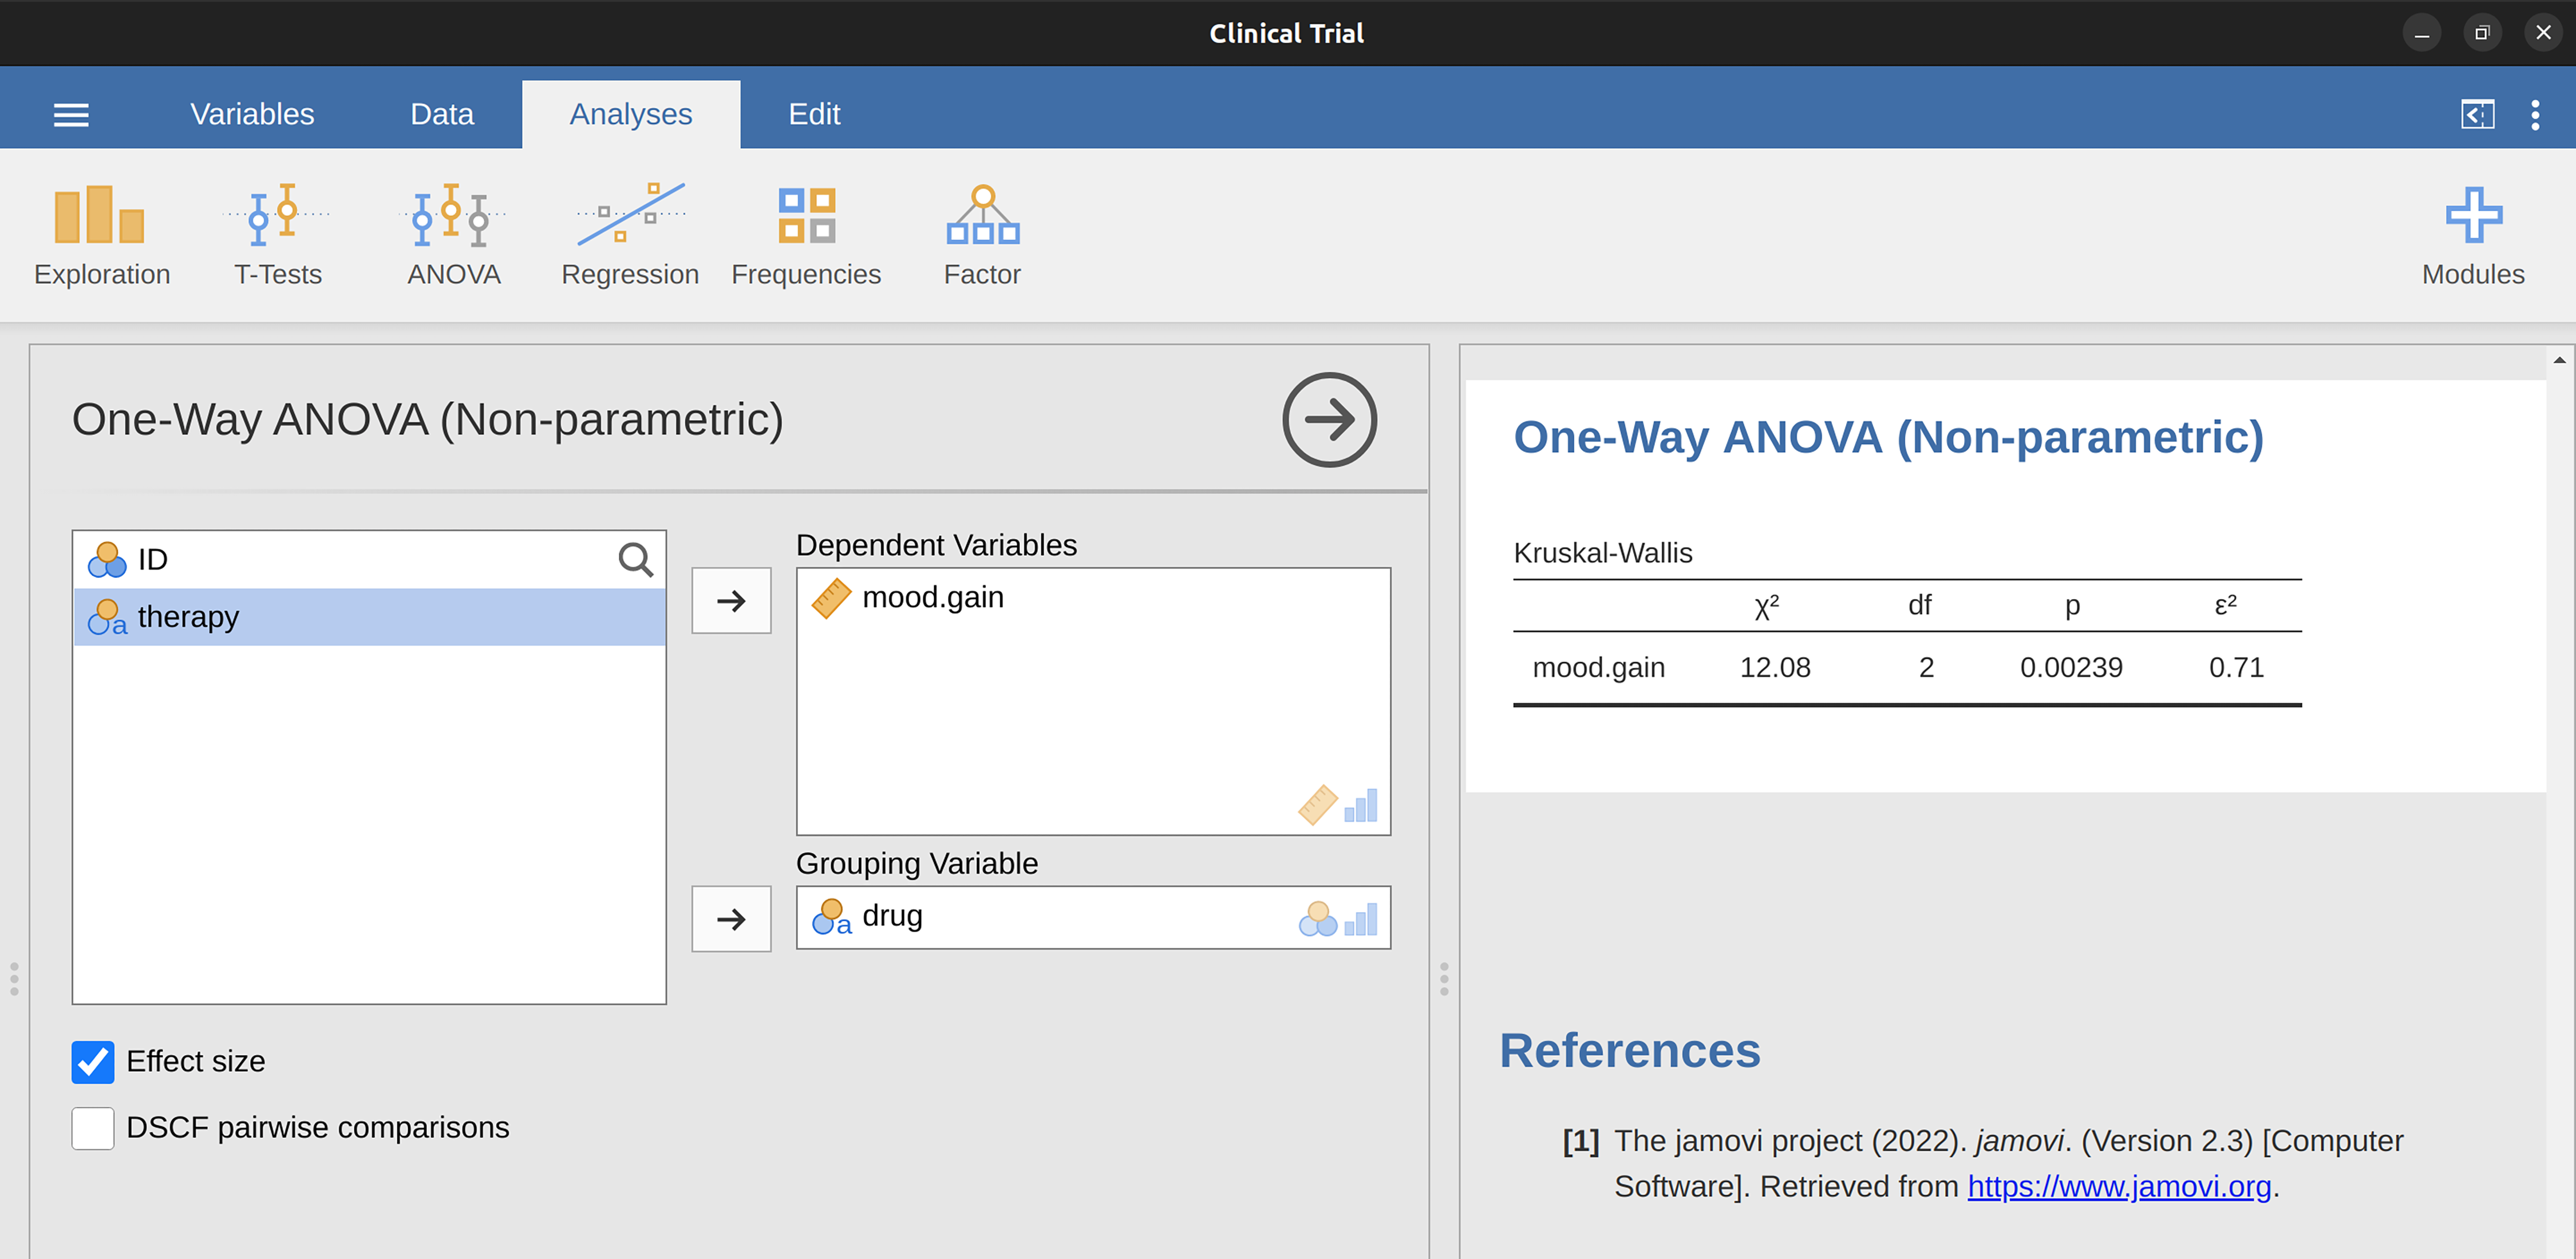
\includegraphics[width=1\textwidth,height=\textheight]{images/fig13-8.png} \hfill{}

\caption{\label{fig-fig13-8}Kruskal-Wallis one-way non-parametric ANOVA
in jamovi}

\end{figure}

\hypertarget{repeated-measures-one-way-anova}{%
\section{Repeated measures one-way
ANOVA}\label{repeated-measures-one-way-anova}}

The one-way repeated measures ANOVA test is a statistical method of
testing for significant differences between three or more groups where
the same participants are used in each group (or each participant is
closely matched with participants in other experimental groups). For
this reason, there should always be an equal number of scores (data
points) in each experimental group. This type of design and analysis can
also be called a ``related ANOVA'' or a ``within subjects ANOVA''.

The logic behind a repeated measures ANOVA is very similar to that of an
independent ANOVA (sometimes called a ``between subjects'' ANOVA).
You'll remember that earlier we showed that in a between subjects ANOVA
total variability is partitioned into between groups variability
(\(SS_b\)) and within groups variability (\(SS_w\)), and after each is
divided by the respective degrees of freedom to give \(MS_b\) and
\(MS_w\) (see Table 13.1) the \(F\)-ratio is calculated as:

\[F=\frac{MS_b}{MS_w}\]

In a repeated measures ANOVA, the \(F\)-ratio is calculated in a similar
way, but whereas in an independent ANOVA the within-group variability
(\(SS_w\)) is used as the basis for the \(MS_w\) denominator, in a
repeated measures ANOVA the \(SS_w\) is partioned into two parts. As we
are using the same subjects in each group, we can remove the variability
due to the individual differences between subjects (referred to as
\(SS_{subjects}\)) from the within groups variability. We won't go into
too much technical detail about how this is done, but essentially each
subject becomes a level of a factor called subjects. The variability in
this within subjects factor is then calculated in the same way as any
between subjects factor. And then we can subtract \(SS_{subjects}\))
from \(SS_w\) to provide a smaller \(SS_{error}\)) term:

\[\text{Independent ANOVA: } SS_{error} = SS_w\]
\[\text{Repeated Measures ANOVA: } SS_{error} = SS_w - SS_{subjects}\]
This change in \(SS_{error}\) term often leads to a more powerful
statistical test, but this does depend on whether the reduction in the
\(SS_{error}\) more than compensates for the reduction in degrees of
freedom for the error term (as degrees of freedom go from
\((n - k)\)\footnote{\((n - k)\): (number of subjects - number of
  groups)} to \((n - 1)(k - 1)\) (remembering that there are more
subjects in the independent ANOVA design).

\hypertarget{repeated-measures-anova-in-jamovi}{%
\subsection{Repeated measures ANOVA in
jamovi}\label{repeated-measures-anova-in-jamovi}}

First, we need some data. Geschwind (1972) has suggested that the exact
nature of a patient's language deficit following a stroke can be used to
diagnose the specific region of the brain that has been damaged. A
researcher is concerned with identifying the specific communication
difficulties experienced by six patients suffering from Broca's Aphasia
(a language deficit commonly experienced following a stroke)
(Table~\ref{tbl-tab13-12}).

\hypertarget{tbl-tab13-12}{}
 
  \providecommand{\huxb}[2]{\arrayrulecolor[RGB]{#1}\global\arrayrulewidth=#2pt}
  \providecommand{\huxvb}[2]{\color[RGB]{#1}\vrule width #2pt}
  \providecommand{\huxtpad}[1]{\rule{0pt}{#1}}
  \providecommand{\huxbpad}[1]{\rule[-#1]{0pt}{#1}}

\begin{table}[ht]
\caption{\label{tbl-tab13-12}Word recognition task scores in stroke patients }\tabularnewline

\begin{centerbox}
\begin{threeparttable}
\setlength{\tabcolsep}{0pt}
\begin{tabularx}{0.9\textwidth}{p{0.225\textwidth} p{0.225\textwidth} p{0.225\textwidth} p{0.225\textwidth}}


\hhline{>{\huxb{0, 0, 0}{0.4}}->{\huxb{0, 0, 0}{0.4}}->{\huxb{0, 0, 0}{0.4}}->{\huxb{0, 0, 0}{0.4}}-}
\arrayrulecolor{black}

\multicolumn{1}{!{\huxvb{0, 0, 0}{0}}p{0.225\textwidth}!{\huxvb{0, 0, 0}{0}}}{\hspace{0pt}\parbox[b]{0.225\textwidth-0pt-12pt}{\huxtpad{2pt + 1em}\centering \textbf{Participant}\huxbpad{2pt}}} &
\multicolumn{1}{p{0.225\textwidth}!{\huxvb{0, 0, 0}{0}}}{\hspace{12pt}\parbox[b]{0.225\textwidth-12pt-12pt}{\huxtpad{2pt + 1em}\centering \textbf{Speech}\huxbpad{2pt}}} &
\multicolumn{1}{p{0.225\textwidth}!{\huxvb{0, 0, 0}{0}}}{\hspace{12pt}\parbox[b]{0.225\textwidth-12pt-12pt}{\huxtpad{2pt + 1em}\centering \textbf{Conceptual}\huxbpad{2pt}}} &
\multicolumn{1}{p{0.225\textwidth}!{\huxvb{0, 0, 0}{0}}}{\hspace{12pt}\parbox[b]{0.225\textwidth-12pt-0pt}{\huxtpad{2pt + 1em}\centering \textbf{Syntax}\huxbpad{2pt}}} \tabularnewline[-0.5pt]


\hhline{>{\huxb{0, 0, 0}{0.4}}->{\huxb{0, 0, 0}{0.4}}->{\huxb{0, 0, 0}{0.4}}->{\huxb{0, 0, 0}{0.4}}-}
\arrayrulecolor{black}

\multicolumn{1}{!{\huxvb{0, 0, 0}{0}}p{0.225\textwidth}!{\huxvb{0, 0, 0}{0}}}{\hspace{0pt}\parbox[b]{0.225\textwidth-0pt-12pt}{\huxtpad{2pt + 1em}\centering 1\huxbpad{2pt}}} &
\multicolumn{1}{p{0.225\textwidth}!{\huxvb{0, 0, 0}{0}}}{\hspace{12pt}\parbox[b]{0.225\textwidth-12pt-12pt}{\huxtpad{2pt + 1em}\centering 8\huxbpad{2pt}}} &
\multicolumn{1}{p{0.225\textwidth}!{\huxvb{0, 0, 0}{0}}}{\hspace{12pt}\parbox[b]{0.225\textwidth-12pt-12pt}{\huxtpad{2pt + 1em}\centering 7\huxbpad{2pt}}} &
\multicolumn{1}{p{0.225\textwidth}!{\huxvb{0, 0, 0}{0}}}{\hspace{12pt}\parbox[b]{0.225\textwidth-12pt-0pt}{\huxtpad{2pt + 1em}\centering 6\huxbpad{2pt}}} \tabularnewline[-0.5pt]


\hhline{}
\arrayrulecolor{black}

\multicolumn{1}{!{\huxvb{0, 0, 0}{0}}p{0.225\textwidth}!{\huxvb{0, 0, 0}{0}}}{\hspace{0pt}\parbox[b]{0.225\textwidth-0pt-12pt}{\huxtpad{2pt + 1em}\centering 2\huxbpad{2pt}}} &
\multicolumn{1}{p{0.225\textwidth}!{\huxvb{0, 0, 0}{0}}}{\hspace{12pt}\parbox[b]{0.225\textwidth-12pt-12pt}{\huxtpad{2pt + 1em}\centering 7\huxbpad{2pt}}} &
\multicolumn{1}{p{0.225\textwidth}!{\huxvb{0, 0, 0}{0}}}{\hspace{12pt}\parbox[b]{0.225\textwidth-12pt-12pt}{\huxtpad{2pt + 1em}\centering 8\huxbpad{2pt}}} &
\multicolumn{1}{p{0.225\textwidth}!{\huxvb{0, 0, 0}{0}}}{\hspace{12pt}\parbox[b]{0.225\textwidth-12pt-0pt}{\huxtpad{2pt + 1em}\centering 6\huxbpad{2pt}}} \tabularnewline[-0.5pt]


\hhline{}
\arrayrulecolor{black}

\multicolumn{1}{!{\huxvb{0, 0, 0}{0}}p{0.225\textwidth}!{\huxvb{0, 0, 0}{0}}}{\hspace{0pt}\parbox[b]{0.225\textwidth-0pt-12pt}{\huxtpad{2pt + 1em}\centering 3\huxbpad{2pt}}} &
\multicolumn{1}{p{0.225\textwidth}!{\huxvb{0, 0, 0}{0}}}{\hspace{12pt}\parbox[b]{0.225\textwidth-12pt-12pt}{\huxtpad{2pt + 1em}\centering 9\huxbpad{2pt}}} &
\multicolumn{1}{p{0.225\textwidth}!{\huxvb{0, 0, 0}{0}}}{\hspace{12pt}\parbox[b]{0.225\textwidth-12pt-12pt}{\huxtpad{2pt + 1em}\centering 5\huxbpad{2pt}}} &
\multicolumn{1}{p{0.225\textwidth}!{\huxvb{0, 0, 0}{0}}}{\hspace{12pt}\parbox[b]{0.225\textwidth-12pt-0pt}{\huxtpad{2pt + 1em}\centering 3\huxbpad{2pt}}} \tabularnewline[-0.5pt]


\hhline{}
\arrayrulecolor{black}

\multicolumn{1}{!{\huxvb{0, 0, 0}{0}}p{0.225\textwidth}!{\huxvb{0, 0, 0}{0}}}{\hspace{0pt}\parbox[b]{0.225\textwidth-0pt-12pt}{\huxtpad{2pt + 1em}\centering 4\huxbpad{2pt}}} &
\multicolumn{1}{p{0.225\textwidth}!{\huxvb{0, 0, 0}{0}}}{\hspace{12pt}\parbox[b]{0.225\textwidth-12pt-12pt}{\huxtpad{2pt + 1em}\centering 5\huxbpad{2pt}}} &
\multicolumn{1}{p{0.225\textwidth}!{\huxvb{0, 0, 0}{0}}}{\hspace{12pt}\parbox[b]{0.225\textwidth-12pt-12pt}{\huxtpad{2pt + 1em}\centering 4\huxbpad{2pt}}} &
\multicolumn{1}{p{0.225\textwidth}!{\huxvb{0, 0, 0}{0}}}{\hspace{12pt}\parbox[b]{0.225\textwidth-12pt-0pt}{\huxtpad{2pt + 1em}\centering 5\huxbpad{2pt}}} \tabularnewline[-0.5pt]


\hhline{}
\arrayrulecolor{black}

\multicolumn{1}{!{\huxvb{0, 0, 0}{0}}p{0.225\textwidth}!{\huxvb{0, 0, 0}{0}}}{\hspace{0pt}\parbox[b]{0.225\textwidth-0pt-12pt}{\huxtpad{2pt + 1em}\centering 5\huxbpad{2pt}}} &
\multicolumn{1}{p{0.225\textwidth}!{\huxvb{0, 0, 0}{0}}}{\hspace{12pt}\parbox[b]{0.225\textwidth-12pt-12pt}{\huxtpad{2pt + 1em}\centering 6\huxbpad{2pt}}} &
\multicolumn{1}{p{0.225\textwidth}!{\huxvb{0, 0, 0}{0}}}{\hspace{12pt}\parbox[b]{0.225\textwidth-12pt-12pt}{\huxtpad{2pt + 1em}\centering 6\huxbpad{2pt}}} &
\multicolumn{1}{p{0.225\textwidth}!{\huxvb{0, 0, 0}{0}}}{\hspace{12pt}\parbox[b]{0.225\textwidth-12pt-0pt}{\huxtpad{2pt + 1em}\centering 2\huxbpad{2pt}}} \tabularnewline[-0.5pt]


\hhline{}
\arrayrulecolor{black}

\multicolumn{1}{!{\huxvb{0, 0, 0}{0}}p{0.225\textwidth}!{\huxvb{0, 0, 0}{0}}}{\hspace{0pt}\parbox[b]{0.225\textwidth-0pt-12pt}{\huxtpad{2pt + 1em}\centering 6\huxbpad{2pt}}} &
\multicolumn{1}{p{0.225\textwidth}!{\huxvb{0, 0, 0}{0}}}{\hspace{12pt}\parbox[b]{0.225\textwidth-12pt-12pt}{\huxtpad{2pt + 1em}\centering 8\huxbpad{2pt}}} &
\multicolumn{1}{p{0.225\textwidth}!{\huxvb{0, 0, 0}{0}}}{\hspace{12pt}\parbox[b]{0.225\textwidth-12pt-12pt}{\huxtpad{2pt + 1em}\centering 7\huxbpad{2pt}}} &
\multicolumn{1}{p{0.225\textwidth}!{\huxvb{0, 0, 0}{0}}}{\hspace{12pt}\parbox[b]{0.225\textwidth-12pt-0pt}{\huxtpad{2pt + 1em}\centering 4\huxbpad{2pt}}} \tabularnewline[-0.5pt]


\hhline{>{\huxb{0, 0, 0}{0.4}}->{\huxb{0, 0, 0}{0.4}}->{\huxb{0, 0, 0}{0.4}}->{\huxb{0, 0, 0}{0.4}}-}
\arrayrulecolor{black}
\end{tabularx} 

\end{threeparttable}\par\end{centerbox}

\end{table}
 

The patients were required to complete three word recognition tasks. On
the first (speech production) task, patients were required to repeat
single words read out aloud by the researcher. On the second
(conceptual) task, designed to test word comprehension, patients were
required to match a series of pictures with their correct name. On the
third (syntax) task, designed to test knowledge of correct word order,
patients were asked to reorder syntactically incorrect sentences. Each
patient completed all three tasks. The order in which patients attempted
the tasks was counterbalanced between participants. Each task consisted
of a series of 10 attempts. The number of attempts successfully
completed by each patient are shown in Table~\ref{tbl-tab13-11}. Enter
these data into jamovi ready for analysis (or take a short-cut and load
up the \emph{broca.csv} file).

To perform a one-way related ANOVA in jamovi, open the one-way repeated
measures ANOVA dialogue box, as in Figure~\ref{fig-fig13-9}, via ANOVA -
Repeated Measures ANOVA.

\begin{figure}

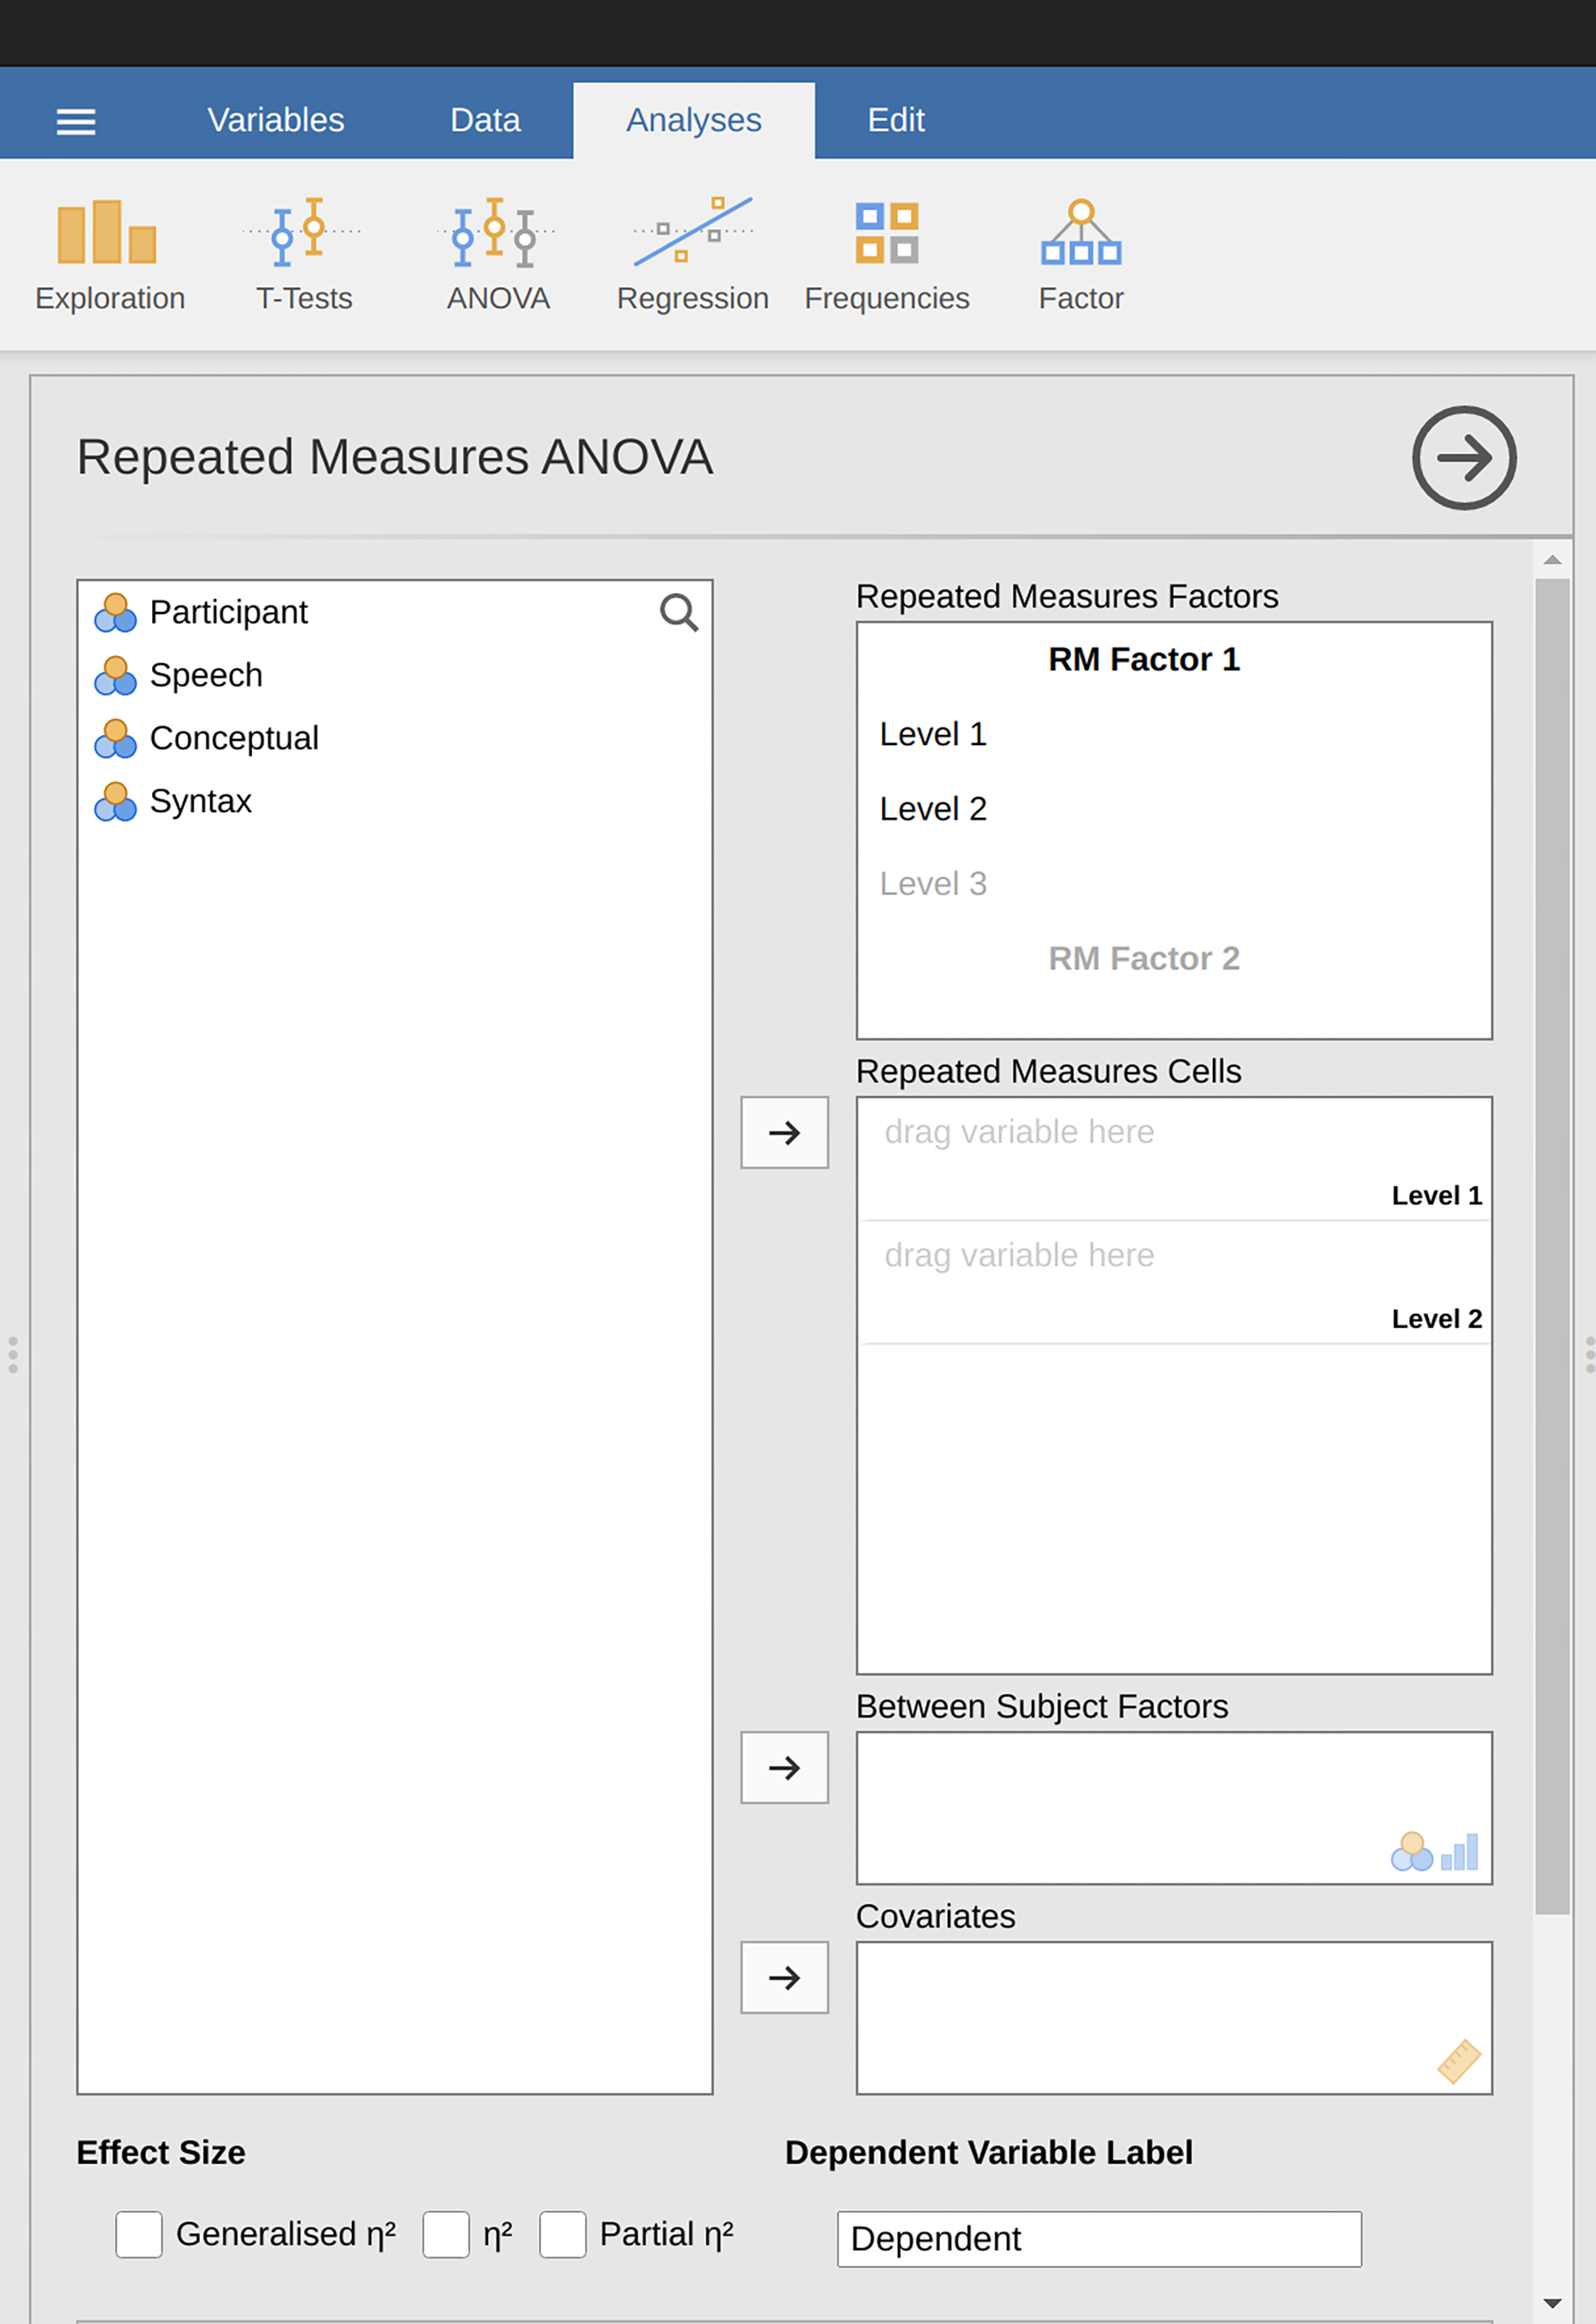
\includegraphics[width=1\textwidth,height=\textheight]{images/fig13-9.png} \hfill{}

\caption{\label{fig-fig13-9}Repeated measures ANOVA dialogue box in
jamovi}

\end{figure}

Then:

\begin{itemize}
\tightlist
\item
  Enter a `Repeated Measures' factor name. This should be a label that
  you choose to describe the conditions repeated by all participants.
  For example, to describe the speech, conceptual and syntax tasks
  completed by all participants a suitable label would be `Task'. Note
  that this new factor name represents the independent variable in the
  analysis.
\item
  Add a third level in the `Repeated Measures Factors' text box, as
  there are three levels representing the three tasks: speech,
  conceptual and syntax. Change the labels of the levels accordingly.
\item
  Then move each of the levels variables across to the `Repeated
  Measures' Cells text box.
\item
  Finally, under the `Assumption Checks' option, tick the `Sphericity
  checks' text box.
\end{itemize}

jamovi output for a one-way repeated measures ANOVA is produced as shown
in Figure~\ref{fig-fig13-10} to Figure~\ref{fig-fig13-13}. The first
output we should look at is Mauchly's Test of Sphericity, which tests
the hypothesis that the variances of the differences between the
conditions are equal (meaning that the spread of difference scores
between the study conditions is approximately the same). In
Figure~\ref{fig-fig13-10} the significance level in Mauchly's test is
\(p = .720\). If Mauchly's test is non-significant (i.e.~\(p > .05\), as
is the case in this analysis) then it is reasonable to conclude that the
variances of the differences are not significantly different (i.e.~they
are roughly equal and sphericity can be assumed).

\begin{figure}

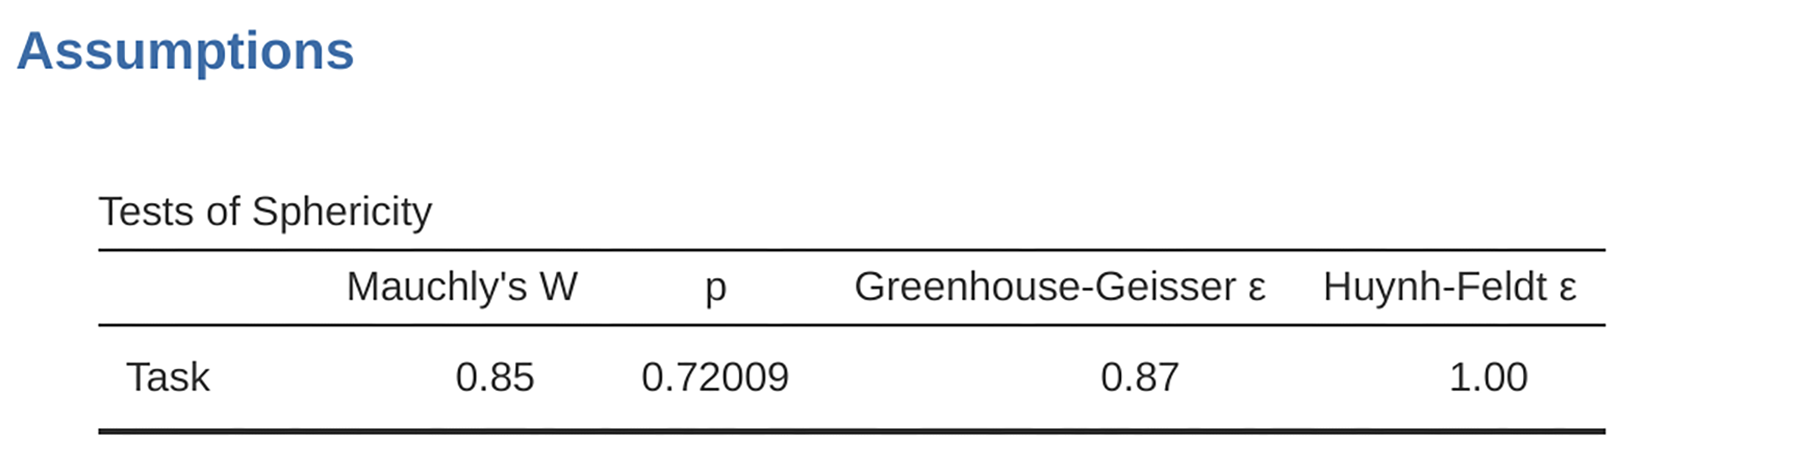
\includegraphics[width=1\textwidth,height=\textheight]{images/fig13-10.png} \hfill{}

\caption{\label{fig-fig13-10}One-way repeated measures ANOVA output --
Mauchly Test of Sphericity}

\end{figure}

If, on the other hand, Mauchly's test had been significant (\(p\)
\textless{} .05) then we would conclude that there are significant
differences between the variance of the differences, and the requirement
of sphericity has not been met. In this case, we should apply a
correction to the \(F\)-value obtained in the one-way related ANOVA
analysis:

\begin{itemize}
\tightlist
\item
  If the Greenhouse-Geisser value in the ``Tests of Sphericity'' table
  is \textgreater{} .75 then you should use the Huynh-Feldt correction
\item
  But if the Greenhouse-Geisser value is \textless{} .75, then you
  should use the Greenhouse-Geisser correction.
\end{itemize}

Both these corrected \(F\)-values can be specified in the `Sphericity
Corrections' check boxes under the `Assumption Checks' options, and the
corrected \(F\)-values are then shown in the results table, as in Figure
\textbf{13.11}.

\begin{figure}

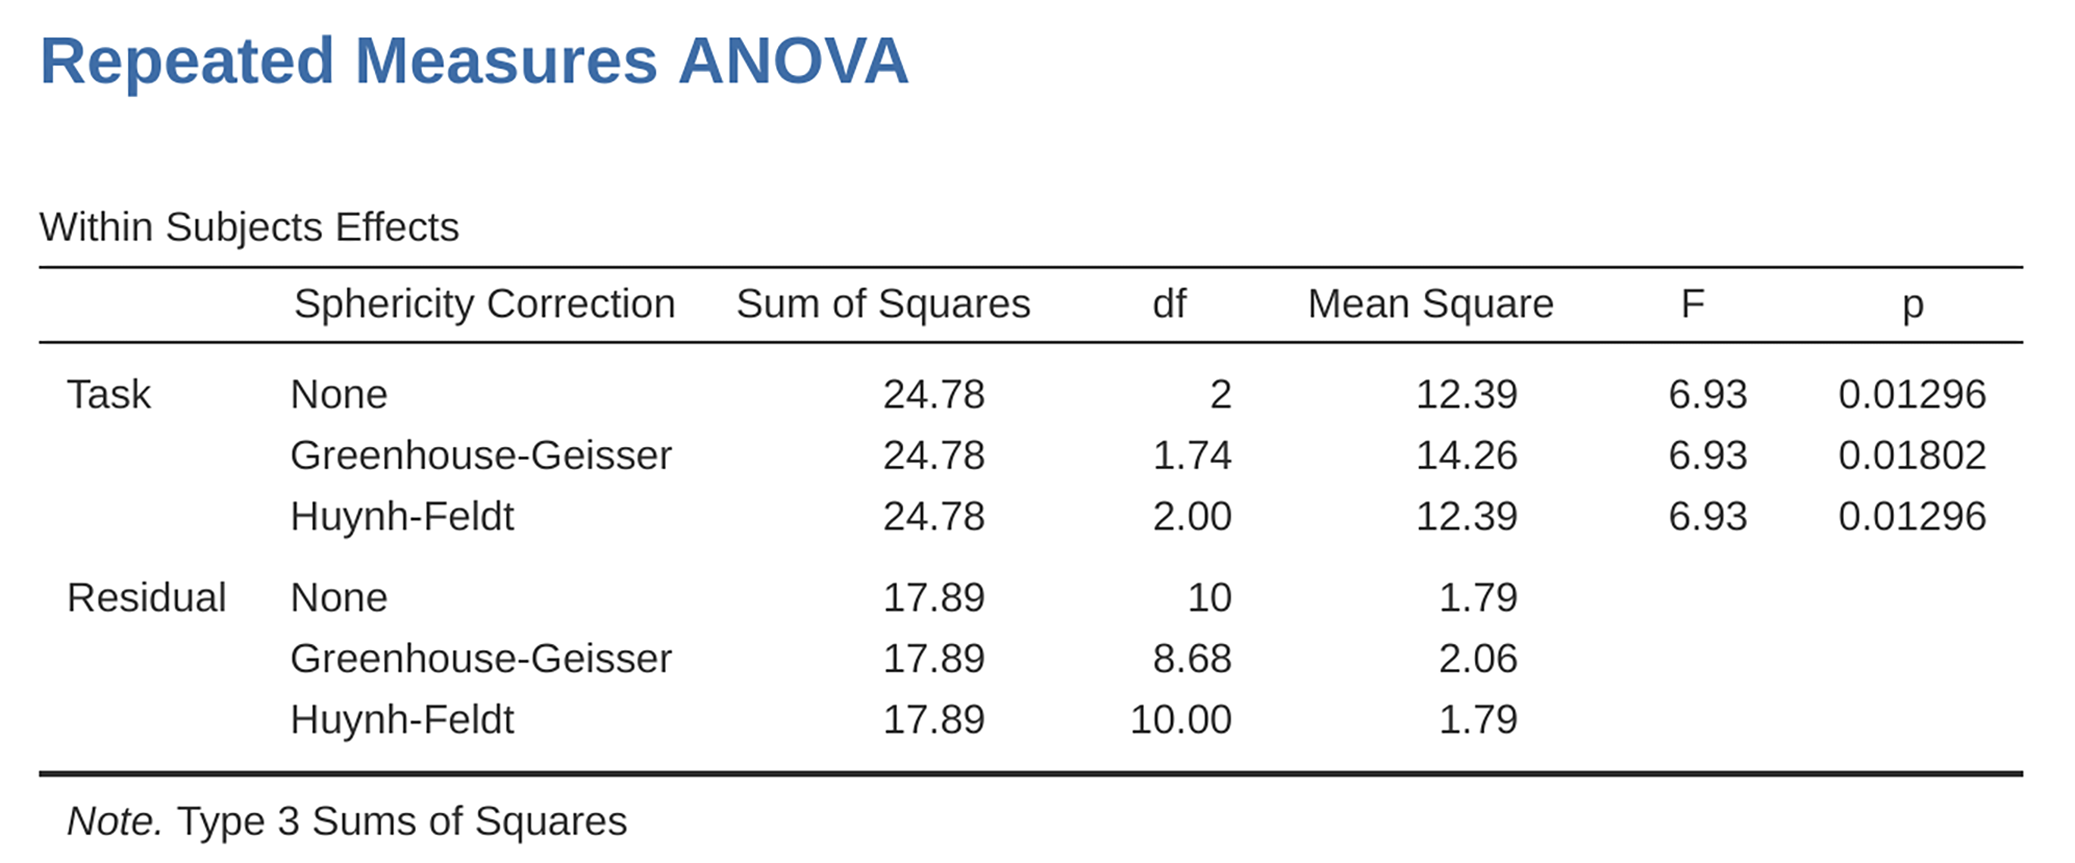
\includegraphics[width=1\textwidth,height=\textheight]{images/fig13-11.png} \hfill{}

\caption{\label{fig-fig13-11}One-way repeated measures ANOVA output --
Tests of Within Subjects Effects}

\end{figure}

In our analysis, we saw that the significance of Mauchly's Test of
Sphericity was \(p = .720\) (i.e., \(p > 0.05)\). So, this means we can
assume that the requirement of sphericity has been met so no correction
to the \(F\)-value is needed. Therefore, we can use the `None'
Sphericity Correction output values for the repeated measure `Task':
\(F = 6.93\), \(df = 2\), \(p = .013\), and we can conclude that the
number of tests successfully completed on each language task did vary
significantly depending on whether the task was speech, comprehension or
syntax based (\(F(2, 10) = 6.93\), \(p = .013\)).

Post hoc tests can also be specified in jamovi for repeated measures
ANOVA in the same way as for independent ANOVA. The results are shown in
Figure~\ref{fig-fig13-12}. These indicate that there is a significant
difference between Speech and Syntax, but not between other levels.

\begin{figure}

\includegraphics[width=1\textwidth,height=\textheight]{images/fig13-12.png} \hfill{}

\caption{\label{fig-fig13-12}Post hoc tests in repeated measures ANOVA
in jamovi}

\end{figure}

Descriptive statistics (marginal means) can be reviewed to help
interpret the results, produced in the jamovi output as in
Figure~\ref{fig-fig13-13}. Comparison of the mean number of trials
successfully completed by participants shows that Broca's Aphasics
perform reasonably well on speech production (mean = 7.17) and language
comprehension (mean = 6.17) tasks. However, their performance was
considerably worse on the syntax task (mean = 4.33), with a significant
difference in post hoc tests between Speech and Syntax task performance.

\begin{figure}

\includegraphics[width=1\textwidth,height=\textheight]{images/fig13-13.png} \hfill{}

\caption{\label{fig-fig13-13}One-way repeated measures ANOVA output --
Descriptive Statistics}

\end{figure}

\hypertarget{the-friedman-non-parametric-repeated-measures-anova-test}{%
\section{The Friedman non-parametric repeated measures ANOVA
test}\label{the-friedman-non-parametric-repeated-measures-anova-test}}

The Friedman test is a non-parametric version of a repeated measures
ANOVA and can be used instead of the Kruskal-Wallis test when testing
for differences between three or more groups where the same participants
are in each group, or each participant is closely matched with
participants in other conditions. If the dependent variable is ordinal,
or if the assumption of normality is not met, then the Friedman test can
be used.

As with the Kruskal-Wallis test, the underlying mathematics is
complicated, and won't be presented here. For the purpose of this book,
it is sufficient to note that jamovi calculates the tie-corrected
version of the Friedman test, and in Figure~\ref{fig-fig13-14} there is
an example using the Broca's Aphasia data we have already looked at.

\begin{figure}

\includegraphics[width=1\textwidth,height=\textheight]{images/fig13-14.png} \hfill{}

\caption{\label{fig-fig13-14}The `Repeated Measures ANOVA
(Non-parametric)' dialogue box and results in jamovi}

\end{figure}

It's pretty straightforward to run a Friedman test in jamovi. Just
select `Analyses - ANOVA - Repeated Measures ANOVA (Non-parametric)' as
in Figure~\ref{fig-fig13-14}. Then highlight and transfer the names of
the repeated measures variables you wish to compare (Speech, Conceptual,
Syntax) into the `Measures:' text box. To produce descriptive statistics
(means and medians) for the three repeated measures variables, click on
the `Descriptives' button.

The jamovi results show descriptive statistics, chi-square value,
degrees of freedom, and the \(p\)-value (Figure~\ref{fig-fig13-14}).
Since the \(p\)-value is less than the level conventionally used to
determine significance (\(p < .05\)), we can conclude that Broca's
Aphasics perform reasonably well on speech production (median = 7.5) and
language comprehension (median = 6.5) tasks. However, their performance
was considerably worse on the syntax task (median = 4.5), with a
significant difference in post hoc tests between Speech and Syntax task
performance.

\hypertarget{sec-On-the-relationship-between-ANOVA-and-the-Student-t-test}{%
\section{\texorpdfstring{On the relationship between ANOVA and the
Student
\(t\)-test}{On the relationship between ANOVA and the Student t-test}}\label{sec-On-the-relationship-between-ANOVA-and-the-Student-t-test}}

There's one last thing I want to point out before finishing. It's
something that a lot of people find kind of surprising, but it's worth
knowing about. An ANOVA with two groups is identical to the Student
\(t\)-test. No, really. It's not just that they are similar, but they
are actually equivalent in every meaningful way. I won't try to prove
that this is always true, but I will show you a single concrete
demonstration. Suppose that, instead of running an ANOVA on our
mood.gain \textasciitilde{} drug model, let's instead do it using
therapy as the predictor. If we run this ANOVA we get an \(F\) statistic
of \(F(1,16) = 1.71\), and a \(p\)-value = \(0.21\). Since we only have
two groups, I didn't actually need to resort to an ANOVA, I could have
just decided to run a Student \(t\)-test. So let's see what happens when
I do that: I get a \(t\) statistic of \(t(16) = -1.3068\) and a
\(p\)-value = 0.21. Curiously, the \(p\)-values are identical. Once
again we obtain a value of \(p = .21\). But what about the test
statistic? Having run a \(t\)-test instead of an ANOVA, we get a
somewhat different answer, namely \(t(16) = -1.3068\). However, there is
a fairly straightforward relationship here. If we square the \(t\)
statistic then we get the \(F\) statistic from before:
\$-1.3068\^{}\{2\} = 1.7077\$4.

\hypertarget{summary-1}{%
\section{Summary}\label{summary-1}}

There's a fair bit covered in this chapter, but there's still a lot
missing\footnote{As with all of the chapters in this book, there are
  quite a few different sources that I've relied upon, but the one
  stand-out text that I've been most heavily influenced by is Sahai \&
  Ageel (2000). It's not a good book for beginners, but it's an
  excellent book for more advanced readers who are interested in
  understanding the mathematics behind ANOVA.}. Most obviously, I
haven't discussed how to run an ANOVA when you are interested in more
than one grouping variable, but that will be discussed in a lot of
detail in Chapter~\ref{sec-Factorial-ANOVA}. In terms of what we have
discussed, the key topics were:

\begin{itemize}
\tightlist
\item
  The basic logic behind \protect\hyperlink{sec-How-ANOVA-works}{How
  ANOVA works} and
  \protect\hyperlink{running-an-anova-in-jamovi}{Running an ANOVA in
  jamovi}.
\item
  How to compute an \protect\hyperlink{effect-size}{Effect size} for an
  ANOVA.
\item
  \protect\hyperlink{multiple-comparisons-and-post-hoc-tests}{Multiple
  comparisons and post hoc tests} for multiple testing.
\item
  \protect\hyperlink{the-assumptions-of-one-way-anova}{The assumptions
  of one-way ANOVA}.
\item
  \protect\hyperlink{sec-Checking-the-homogeneity-of-variance-assumption}{Checking
  the homogeneity of variance assumption} and what to do if it is
  violated:
  \protect\hyperlink{removing-the-homogeneity-of-variance-assumption}{Removing
  the homogeneity of variance assumption}.
\item
  \protect\hyperlink{sec-Checking-the-normality-assumption}{Checking the
  normality assumption} and what to do if it is violated:
  \protect\hyperlink{removing-the-normality-assumption}{Removing the
  normality assumption}.
\item
  \protect\hyperlink{repeated-measures-one-way-anova}{Repeated measures
  one-way ANOVA} and the non-parametric equivalent,
  \protect\hyperlink{the-friedman-non-parametric-repeated-measures-anova-test}{The
  Friedman non-parametric repeated measures ANOVA test}.
\end{itemize}

\bookmarksetup{startatroot}

\hypertarget{sec-Factorial-ANOVA}{%
\chapter{Factorial ANOVA}\label{sec-Factorial-ANOVA}}

Over the course of the last few chapters we have done quite a lot. We
have looked at statistical tests you can use when you have one nominal
predictor variable with two groups (e.g.~the \(t\)-test in
\textbf{?@sec-Comparing-two-means}) or with three or more groups
(Chapter~\ref{sec-Comparing-several-means-one-way-ANOVA}).
Chapter~\ref{sec-Correlation-and-linear-regression} introduced a
powerful new idea, that is building statistical models with multiple
continuous predictor variables used to explain a single outcome
variable. For instance, a regression model could be used to predict the
number of errors a student makes in a reading comprehension test based
on the number of hours they studied for the test and their score on a
standardised IQ test.

The goal in this chapter is to extend the idea of using multiple
predictors into the ANOVA framework. For instance, suppose we were
interested in using the reading comprehension test to measure student
achievements in three different schools, and we suspect that girls and
boys are developing at different rates (and so would be expected to have
different performance on average). Each student is classified in two
different ways: on the basis of their gender and on the basis of their
school. What we'd like to do is analyse the reading comprehension scores
in terms of both of these grouping variables. The tool for doing so is
generically referred to as \textbf{factorial ANOVA}. However, since we
have two grouping variables, we sometimes refer to the analysis as a
two-way ANOVA, in contrast to the one-way ANOVAs that we ran in
Chapter~\ref{sec-Comparing-several-means-one-way-ANOVA}.

\hypertarget{factorial-anova-1-balanced-designs-focus-on-main-effects}{%
\section{Factorial ANOVA 1: balanced designs, focus on main
effects}\label{factorial-anova-1-balanced-designs-focus-on-main-effects}}

When we discussed analysis of variance in
Chapter~\ref{sec-Comparing-several-means-one-way-ANOVA}, we assumed a
fairly simple experimental design. Each person is in one of several
groups and we want to know whether these groups have different mean
scores on some outcome variable. In this section, I'll discuss a broader
class of experimental designs known as \textbf{factorial designs}, in
which we have more than one grouping variable. I gave one example of how
this kind of design might arise above. Another example appears in
Chapter~\ref{sec-Comparing-several-means-one-way-ANOVA} in which we were
looking at the effect of different drugs on the mood.gain experienced by
each person. In that chapter we did find a significant effect of drug,
but at the end of the chapter we also ran an analysis to see if there
was an effect of therapy. We didn't find one, but there's something a
bit worrying about trying to run two separate analyses trying to predict
the same outcome. Maybe there actually is an effect of therapy on mood
gain, but we couldn't find it because it was being ``hidden'' by the
effect of drug? In other words, we're going to want to run a single
analysis that includes both drug and therapy as predictors. For this
analysis each person is cross-classified by the drug they were given (a
factor with 3 levels) and what therapy they received (a factor with 2
levels). We refer to this as a \(3 \times 2\) factorial design.

If we cross-tabulate drug by therapy, using the `Frequencies' -
`Contingency Tables' analysis in jamovi (see
\textbf{?@sec-Tabulating-and-cross-tabulating-data}), we get the table
shown in Figure~\ref{fig-fig14-1}.

\begin{figure}

\includegraphics[width=1\textwidth,height=\textheight]{images/fig14-1.png} \hfill{}

\caption{\label{fig-fig14-1}jamovi contingency table of drug by therapy}

\end{figure}

As you can see, not only do we have participants corresponding to all
possible combinations of the two factors, indicating that our design is
\textbf{completely crossed}, it turns out that there are an equal number
of people in each group. In other words, we have a balanced design. In
this section I'll talk about how to analyse data from \textbf{balanced}
designs, since this is the simplest case. The story for unbalanced
designs is quite tedious, so we'll put it to one side for the moment.

\hypertarget{sec-What-hypotheses-are-we-testing}{%
\subsection{What hypotheses are we
testing?}\label{sec-What-hypotheses-are-we-testing}}

Like one-way ANOVA, factorial ANOVA is a tool for testing certain types
of hypotheses about population means. So a sensible place to start would
be to be explicit about what our hypotheses actually are. However,
before we can even get to that point, it's really useful to have some
clean and simple notation to describe the population means. Because of
the fact that observations are cross-classified in terms of two
different factors, there are quite a lot of different means that one
might be interested in. To see this, let's start by thinking about all
the different sample means that we can calculate for this kind of
design. Firstly, there's the obvious idea that we might be interested in
this list of group means (Table~\ref{tbl-tab14-1}).

\hypertarget{tbl-tab14-1}{}
 
  \providecommand{\huxb}[2]{\arrayrulecolor[RGB]{#1}\global\arrayrulewidth=#2pt}
  \providecommand{\huxvb}[2]{\color[RGB]{#1}\vrule width #2pt}
  \providecommand{\huxtpad}[1]{\rule{0pt}{#1}}
  \providecommand{\huxbpad}[1]{\rule[-#1]{0pt}{#1}}

\begin{table}[ht]
\caption{\label{tbl-tab14-1}Group means for drug and therapy groups in the \emph{clinicaltrial.csv}
data }\tabularnewline

\begin{centerbox}
\begin{threeparttable}
\setlength{\tabcolsep}{0pt}
\begin{tabularx}{0.9\textwidth}{p{0.3\textwidth} p{0.3\textwidth} p{0.3\textwidth}}


\hhline{>{\huxb{0, 0, 0}{0.4}}->{\huxb{0, 0, 0}{0.4}}->{\huxb{0, 0, 0}{0.4}}-}
\arrayrulecolor{black}

\multicolumn{1}{!{\huxvb{0, 0, 0}{0}}p{0.3\textwidth}!{\huxvb{0, 0, 0}{0}}}{\hspace{0pt}\parbox[b]{0.3\textwidth-0pt-12pt}{\huxtpad{2pt + 1em}\centering \textbf{drug}\huxbpad{2pt}}} &
\multicolumn{1}{p{0.3\textwidth}!{\huxvb{0, 0, 0}{0}}}{\hspace{12pt}\parbox[b]{0.3\textwidth-12pt-12pt}{\huxtpad{2pt + 1em}\centering \textbf{therapy}\huxbpad{2pt}}} &
\multicolumn{1}{p{0.3\textwidth}!{\huxvb{0, 0, 0}{0}}}{\hspace{12pt}\parbox[b]{0.3\textwidth-12pt-0pt}{\huxtpad{2pt + 1em}\centering \textbf{mood.gain}\huxbpad{2pt}}} \tabularnewline[-0.5pt]


\hhline{>{\huxb{0, 0, 0}{0.4}}->{\huxb{0, 0, 0}{0.4}}->{\huxb{0, 0, 0}{0.4}}-}
\arrayrulecolor{black}

\multicolumn{1}{!{\huxvb{0, 0, 0}{0}}p{0.3\textwidth}!{\huxvb{0, 0, 0}{0}}}{\hspace{0pt}\parbox[b]{0.3\textwidth-0pt-12pt}{\huxtpad{2pt + 1em}\centering placebo\huxbpad{2pt}}} &
\multicolumn{1}{p{0.3\textwidth}!{\huxvb{0, 0, 0}{0}}}{\hspace{12pt}\parbox[b]{0.3\textwidth-12pt-12pt}{\huxtpad{2pt + 1em}\centering no.therapy\huxbpad{2pt}}} &
\multicolumn{1}{p{0.3\textwidth}!{\huxvb{0, 0, 0}{0}}}{\hspace{12pt}\parbox[b]{0.3\textwidth-12pt-0pt}{\huxtpad{2pt + 1em}\centering 0.30\huxbpad{2pt}}} \tabularnewline[-0.5pt]


\hhline{}
\arrayrulecolor{black}

\multicolumn{1}{!{\huxvb{0, 0, 0}{0}}p{0.3\textwidth}!{\huxvb{0, 0, 0}{0}}}{\hspace{0pt}\parbox[b]{0.3\textwidth-0pt-12pt}{\huxtpad{2pt + 1em}\centering anxifree\huxbpad{2pt}}} &
\multicolumn{1}{p{0.3\textwidth}!{\huxvb{0, 0, 0}{0}}}{\hspace{12pt}\parbox[b]{0.3\textwidth-12pt-12pt}{\huxtpad{2pt + 1em}\centering no.therapy\huxbpad{2pt}}} &
\multicolumn{1}{p{0.3\textwidth}!{\huxvb{0, 0, 0}{0}}}{\hspace{12pt}\parbox[b]{0.3\textwidth-12pt-0pt}{\huxtpad{2pt + 1em}\centering 0.40\huxbpad{2pt}}} \tabularnewline[-0.5pt]


\hhline{}
\arrayrulecolor{black}

\multicolumn{1}{!{\huxvb{0, 0, 0}{0}}p{0.3\textwidth}!{\huxvb{0, 0, 0}{0}}}{\hspace{0pt}\parbox[b]{0.3\textwidth-0pt-12pt}{\huxtpad{2pt + 1em}\centering joyzepam\huxbpad{2pt}}} &
\multicolumn{1}{p{0.3\textwidth}!{\huxvb{0, 0, 0}{0}}}{\hspace{12pt}\parbox[b]{0.3\textwidth-12pt-12pt}{\huxtpad{2pt + 1em}\centering no.therapy\huxbpad{2pt}}} &
\multicolumn{1}{p{0.3\textwidth}!{\huxvb{0, 0, 0}{0}}}{\hspace{12pt}\parbox[b]{0.3\textwidth-12pt-0pt}{\huxtpad{2pt + 1em}\centering 1.47\huxbpad{2pt}}} \tabularnewline[-0.5pt]


\hhline{}
\arrayrulecolor{black}

\multicolumn{1}{!{\huxvb{0, 0, 0}{0}}p{0.3\textwidth}!{\huxvb{0, 0, 0}{0}}}{\hspace{0pt}\parbox[b]{0.3\textwidth-0pt-12pt}{\huxtpad{2pt + 1em}\centering placebo\huxbpad{2pt}}} &
\multicolumn{1}{p{0.3\textwidth}!{\huxvb{0, 0, 0}{0}}}{\hspace{12pt}\parbox[b]{0.3\textwidth-12pt-12pt}{\huxtpad{2pt + 1em}\centering CBT\huxbpad{2pt}}} &
\multicolumn{1}{p{0.3\textwidth}!{\huxvb{0, 0, 0}{0}}}{\hspace{12pt}\parbox[b]{0.3\textwidth-12pt-0pt}{\huxtpad{2pt + 1em}\centering 0.60\huxbpad{2pt}}} \tabularnewline[-0.5pt]


\hhline{}
\arrayrulecolor{black}

\multicolumn{1}{!{\huxvb{0, 0, 0}{0}}p{0.3\textwidth}!{\huxvb{0, 0, 0}{0}}}{\hspace{0pt}\parbox[b]{0.3\textwidth-0pt-12pt}{\huxtpad{2pt + 1em}\centering anxifree\huxbpad{2pt}}} &
\multicolumn{1}{p{0.3\textwidth}!{\huxvb{0, 0, 0}{0}}}{\hspace{12pt}\parbox[b]{0.3\textwidth-12pt-12pt}{\huxtpad{2pt + 1em}\centering CBT\huxbpad{2pt}}} &
\multicolumn{1}{p{0.3\textwidth}!{\huxvb{0, 0, 0}{0}}}{\hspace{12pt}\parbox[b]{0.3\textwidth-12pt-0pt}{\huxtpad{2pt + 1em}\centering 1.03\huxbpad{2pt}}} \tabularnewline[-0.5pt]


\hhline{}
\arrayrulecolor{black}

\multicolumn{1}{!{\huxvb{0, 0, 0}{0}}p{0.3\textwidth}!{\huxvb{0, 0, 0}{0}}}{\hspace{0pt}\parbox[b]{0.3\textwidth-0pt-12pt}{\huxtpad{2pt + 1em}\centering joyzepam\huxbpad{2pt}}} &
\multicolumn{1}{p{0.3\textwidth}!{\huxvb{0, 0, 0}{0}}}{\hspace{12pt}\parbox[b]{0.3\textwidth-12pt-12pt}{\huxtpad{2pt + 1em}\centering CBT\huxbpad{2pt}}} &
\multicolumn{1}{p{0.3\textwidth}!{\huxvb{0, 0, 0}{0}}}{\hspace{12pt}\parbox[b]{0.3\textwidth-12pt-0pt}{\huxtpad{2pt + 1em}\centering 1.50\huxbpad{2pt}}} \tabularnewline[-0.5pt]


\hhline{>{\huxb{0, 0, 0}{0.4}}->{\huxb{0, 0, 0}{0.4}}->{\huxb{0, 0, 0}{0.4}}-}
\arrayrulecolor{black}
\end{tabularx} 

\end{threeparttable}\par\end{centerbox}

\end{table}
 

Now, the next Table (Table~\ref{tbl-tab14-2}) shows a list of the group
means for all possible combinations of the two factors (e.g., people who
received the placebo and no therapy, people who received the placebo
while getting CBT, etc.). It is helpful to organise all these numbers,
plus the marginal and grand means, into a single table which looks like
this:

\hypertarget{tbl-tab14-2}{}
 
  \providecommand{\huxb}[2]{\arrayrulecolor[RGB]{#1}\global\arrayrulewidth=#2pt}
  \providecommand{\huxvb}[2]{\color[RGB]{#1}\vrule width #2pt}
  \providecommand{\huxtpad}[1]{\rule{0pt}{#1}}
  \providecommand{\huxbpad}[1]{\rule[-#1]{0pt}{#1}}

\begin{table}[ht]
\caption{\label{tbl-tab14-2}Group and total means for drug and therapy groups in the clintrial.csv
data }\tabularnewline

\begin{centerbox}
\begin{threeparttable}
\setlength{\tabcolsep}{0pt}
\begin{tabularx}{0.9\textwidth}{p{0.225\textwidth} p{0.225\textwidth} p{0.225\textwidth} p{0.225\textwidth}}


\hhline{>{\huxb{0, 0, 0}{0.4}}->{\huxb{0, 0, 0}{0.4}}->{\huxb{0, 0, 0}{0.4}}->{\huxb{0, 0, 0}{0.4}}-}
\arrayrulecolor{black}

\multicolumn{1}{!{\huxvb{0, 0, 0}{0}}p{0.225\textwidth}!{\huxvb{0, 0, 0}{0}}}{\hspace{0pt}\parbox[b]{0.225\textwidth-0pt-12pt}{\huxtpad{2pt + 1em}\centering \textbf{}\huxbpad{2pt}}} &
\multicolumn{1}{p{0.225\textwidth}!{\huxvb{0, 0, 0}{0}}}{\hspace{12pt}\parbox[b]{0.225\textwidth-12pt-12pt}{\huxtpad{2pt + 1em}\centering \textbf{no therapy}\huxbpad{2pt}}} &
\multicolumn{1}{p{0.225\textwidth}!{\huxvb{0, 0, 0}{0}}}{\hspace{12pt}\parbox[b]{0.225\textwidth-12pt-12pt}{\huxtpad{2pt + 1em}\centering \textbf{CBT}\huxbpad{2pt}}} &
\multicolumn{1}{p{0.225\textwidth}!{\huxvb{0, 0, 0}{0}}}{\hspace{12pt}\parbox[b]{0.225\textwidth-12pt-0pt}{\huxtpad{2pt + 1em}\centering \textbf{total}\huxbpad{2pt}}} \tabularnewline[-0.5pt]


\hhline{>{\huxb{0, 0, 0}{0.4}}->{\huxb{0, 0, 0}{0.4}}->{\huxb{0, 0, 0}{0.4}}->{\huxb{0, 0, 0}{0.4}}-}
\arrayrulecolor{black}

\multicolumn{1}{!{\huxvb{0, 0, 0}{0}}p{0.225\textwidth}!{\huxvb{0, 0, 0}{0}}}{\hspace{0pt}\parbox[b]{0.225\textwidth-0pt-12pt}{\huxtpad{2pt + 1em}\centering placebo\huxbpad{2pt}}} &
\multicolumn{1}{p{0.225\textwidth}!{\huxvb{0, 0, 0}{0}}}{\hspace{12pt}\parbox[b]{0.225\textwidth-12pt-12pt}{\huxtpad{2pt + 1em}\centering 0.30\huxbpad{2pt}}} &
\multicolumn{1}{p{0.225\textwidth}!{\huxvb{0, 0, 0}{0}}}{\hspace{12pt}\parbox[b]{0.225\textwidth-12pt-12pt}{\huxtpad{2pt + 1em}\centering 0.60\huxbpad{2pt}}} &
\multicolumn{1}{p{0.225\textwidth}!{\huxvb{0, 0, 0}{0}}}{\hspace{12pt}\parbox[b]{0.225\textwidth-12pt-0pt}{\huxtpad{2pt + 1em}\centering 0.45\huxbpad{2pt}}} \tabularnewline[-0.5pt]


\hhline{}
\arrayrulecolor{black}

\multicolumn{1}{!{\huxvb{0, 0, 0}{0}}p{0.225\textwidth}!{\huxvb{0, 0, 0}{0}}}{\hspace{0pt}\parbox[b]{0.225\textwidth-0pt-12pt}{\huxtpad{2pt + 1em}\centering anxifree\huxbpad{2pt}}} &
\multicolumn{1}{p{0.225\textwidth}!{\huxvb{0, 0, 0}{0}}}{\hspace{12pt}\parbox[b]{0.225\textwidth-12pt-12pt}{\huxtpad{2pt + 1em}\centering 0.40\huxbpad{2pt}}} &
\multicolumn{1}{p{0.225\textwidth}!{\huxvb{0, 0, 0}{0}}}{\hspace{12pt}\parbox[b]{0.225\textwidth-12pt-12pt}{\huxtpad{2pt + 1em}\centering 1.03\huxbpad{2pt}}} &
\multicolumn{1}{p{0.225\textwidth}!{\huxvb{0, 0, 0}{0}}}{\hspace{12pt}\parbox[b]{0.225\textwidth-12pt-0pt}{\huxtpad{2pt + 1em}\centering 0.72\huxbpad{2pt}}} \tabularnewline[-0.5pt]


\hhline{}
\arrayrulecolor{black}

\multicolumn{1}{!{\huxvb{0, 0, 0}{0}}p{0.225\textwidth}!{\huxvb{0, 0, 0}{0}}}{\hspace{0pt}\parbox[b]{0.225\textwidth-0pt-12pt}{\huxtpad{2pt + 1em}\centering joyzepam\huxbpad{2pt}}} &
\multicolumn{1}{p{0.225\textwidth}!{\huxvb{0, 0, 0}{0}}}{\hspace{12pt}\parbox[b]{0.225\textwidth-12pt-12pt}{\huxtpad{2pt + 1em}\centering 1.47\huxbpad{2pt}}} &
\multicolumn{1}{p{0.225\textwidth}!{\huxvb{0, 0, 0}{0}}}{\hspace{12pt}\parbox[b]{0.225\textwidth-12pt-12pt}{\huxtpad{2pt + 1em}\centering 1.50\huxbpad{2pt}}} &
\multicolumn{1}{p{0.225\textwidth}!{\huxvb{0, 0, 0}{0}}}{\hspace{12pt}\parbox[b]{0.225\textwidth-12pt-0pt}{\huxtpad{2pt + 1em}\centering 1.48\huxbpad{2pt}}} \tabularnewline[-0.5pt]


\hhline{}
\arrayrulecolor{black}

\multicolumn{1}{!{\huxvb{0, 0, 0}{0}}p{0.225\textwidth}!{\huxvb{0, 0, 0}{0}}}{\hspace{0pt}\parbox[b]{0.225\textwidth-0pt-12pt}{\huxtpad{2pt + 1em}\centering total\huxbpad{2pt}}} &
\multicolumn{1}{p{0.225\textwidth}!{\huxvb{0, 0, 0}{0}}}{\hspace{12pt}\parbox[b]{0.225\textwidth-12pt-12pt}{\huxtpad{2pt + 1em}\centering 0.72\huxbpad{2pt}}} &
\multicolumn{1}{p{0.225\textwidth}!{\huxvb{0, 0, 0}{0}}}{\hspace{12pt}\parbox[b]{0.225\textwidth-12pt-12pt}{\huxtpad{2pt + 1em}\centering 1.04\huxbpad{2pt}}} &
\multicolumn{1}{p{0.225\textwidth}!{\huxvb{0, 0, 0}{0}}}{\hspace{12pt}\parbox[b]{0.225\textwidth-12pt-0pt}{\huxtpad{2pt + 1em}\centering 0.88\huxbpad{2pt}}} \tabularnewline[-0.5pt]


\hhline{>{\huxb{0, 0, 0}{0.4}}->{\huxb{0, 0, 0}{0.4}}->{\huxb{0, 0, 0}{0.4}}->{\huxb{0, 0, 0}{0.4}}-}
\arrayrulecolor{black}
\end{tabularx} 

\end{threeparttable}\par\end{centerbox}

\end{table}
 

Now, each of these different means is of course a sample statistic. It's
a quantity that pertains to the specific observations that we've made
during our study. What we want to make inferences about are the
corresponding population parameters. That is, the true means as they
exist within some broader population. Those population means can also be
organised into a similar table, but we'll need a little mathematical
notation to do so (Table~\ref{tbl-tab14-3}). As usual, I'll use the
symbol \(\mu\) to denote a population mean. However, because there are
lots of different means, I'll need to use subscripts to distinguish
between them.

Here's how the notation works. Our table is defined in terms of two
factors. Each row corresponds to a different level of Factor A (in this
case drug), and each column corresponds to a different level of Factor B
(in this case therapy). If we let \(R\) denote the number of rows in the
table, and \(C\) denote the number of columns, we can refer to this as
an \(R \times C\) factorial ANOVA. In this case \(R = 3\) and \(C = 2\).
We'll use lowercase letters to refer to specific rows and columns, so
\(\mu_{rc}\) refers to the population mean associated with the \(r\)-th
level of Factor A (i.e.~row number \(r\)) and the \(c\)-th level of
Factor B (column number c).\footnote{The nice thing about the subscript
  notation is that it generalises nicely. If our experiment had involved
  a third factor, then we could just add a third subscript. In
  principle, the notation extends to as many factors as you might care
  to include, but in this book we'll rarely consider analyses involving
  more than two factors, and never more than three.} So the population
means are now written like in Table~\ref{tbl-tab14-1}:

\hypertarget{tbl-tab14-3}{}
 
  \providecommand{\huxb}[2]{\arrayrulecolor[RGB]{#1}\global\arrayrulewidth=#2pt}
  \providecommand{\huxvb}[2]{\color[RGB]{#1}\vrule width #2pt}
  \providecommand{\huxtpad}[1]{\rule{0pt}{#1}}
  \providecommand{\huxbpad}[1]{\rule[-#1]{0pt}{#1}}

\begin{table}[ht]
\caption{\label{tbl-tab14-3}Notation for population means in a factorial table }\tabularnewline

\begin{centerbox}
\begin{threeparttable}
\setlength{\tabcolsep}{0pt}
\begin{tabularx}{0.9\textwidth}{p{0.225\textwidth} p{0.225\textwidth} p{0.225\textwidth} p{0.225\textwidth}}


\hhline{>{\huxb{0, 0, 0}{0.4}}->{\huxb{0, 0, 0}{0.4}}->{\huxb{0, 0, 0}{0.4}}->{\huxb{0, 0, 0}{0.4}}-}
\arrayrulecolor{black}

\multicolumn{1}{!{\huxvb{0, 0, 0}{0}}p{0.225\textwidth}!{\huxvb{0, 0, 0}{0}}}{\hspace{0pt}\parbox[b]{0.225\textwidth-0pt-12pt}{\huxtpad{2pt + 1em}\centering \textbf{}\huxbpad{2pt}}} &
\multicolumn{1}{p{0.225\textwidth}!{\huxvb{0, 0, 0}{0}}}{\hspace{12pt}\parbox[b]{0.225\textwidth-12pt-12pt}{\huxtpad{2pt + 1em}\centering \textbf{no therapy}\huxbpad{2pt}}} &
\multicolumn{1}{p{0.225\textwidth}!{\huxvb{0, 0, 0}{0}}}{\hspace{12pt}\parbox[b]{0.225\textwidth-12pt-12pt}{\huxtpad{2pt + 1em}\centering \textbf{CBT}\huxbpad{2pt}}} &
\multicolumn{1}{p{0.225\textwidth}!{\huxvb{0, 0, 0}{0}}}{\hspace{12pt}\parbox[b]{0.225\textwidth-12pt-0pt}{\huxtpad{2pt + 1em}\centering \textbf{total}\huxbpad{2pt}}} \tabularnewline[-0.5pt]


\hhline{>{\huxb{0, 0, 0}{0.4}}->{\huxb{0, 0, 0}{0.4}}->{\huxb{0, 0, 0}{0.4}}->{\huxb{0, 0, 0}{0.4}}-}
\arrayrulecolor{black}

\multicolumn{1}{!{\huxvb{0, 0, 0}{0}}p{0.225\textwidth}!{\huxvb{0, 0, 0}{0}}}{\hspace{0pt}\parbox[b]{0.225\textwidth-0pt-12pt}{\huxtpad{2pt + 1em}\centering placebo\huxbpad{2pt}}} &
\multicolumn{1}{p{0.225\textwidth}!{\huxvb{0, 0, 0}{0}}}{\hspace{12pt}\parbox[b]{0.225\textwidth-12pt-12pt}{\huxtpad{2pt + 1em}\centering \( \mu_{11} \)\huxbpad{2pt}}} &
\multicolumn{1}{p{0.225\textwidth}!{\huxvb{0, 0, 0}{0}}}{\hspace{12pt}\parbox[b]{0.225\textwidth-12pt-12pt}{\huxtpad{2pt + 1em}\centering \( \mu_{12} \)\huxbpad{2pt}}} &
\multicolumn{1}{p{0.225\textwidth}!{\huxvb{0, 0, 0}{0}}}{\hspace{12pt}\parbox[b]{0.225\textwidth-12pt-0pt}{\huxtpad{2pt + 1em}\centering \huxbpad{2pt}}} \tabularnewline[-0.5pt]


\hhline{}
\arrayrulecolor{black}

\multicolumn{1}{!{\huxvb{0, 0, 0}{0}}p{0.225\textwidth}!{\huxvb{0, 0, 0}{0}}}{\hspace{0pt}\parbox[b]{0.225\textwidth-0pt-12pt}{\huxtpad{2pt + 1em}\centering anxifree\huxbpad{2pt}}} &
\multicolumn{1}{p{0.225\textwidth}!{\huxvb{0, 0, 0}{0}}}{\hspace{12pt}\parbox[b]{0.225\textwidth-12pt-12pt}{\huxtpad{2pt + 1em}\centering \( \mu_{21} \)\huxbpad{2pt}}} &
\multicolumn{1}{p{0.225\textwidth}!{\huxvb{0, 0, 0}{0}}}{\hspace{12pt}\parbox[b]{0.225\textwidth-12pt-12pt}{\huxtpad{2pt + 1em}\centering \( \mu_{22} \)\huxbpad{2pt}}} &
\multicolumn{1}{p{0.225\textwidth}!{\huxvb{0, 0, 0}{0}}}{\hspace{12pt}\parbox[b]{0.225\textwidth-12pt-0pt}{\huxtpad{2pt + 1em}\centering \huxbpad{2pt}}} \tabularnewline[-0.5pt]


\hhline{}
\arrayrulecolor{black}

\multicolumn{1}{!{\huxvb{0, 0, 0}{0}}p{0.225\textwidth}!{\huxvb{0, 0, 0}{0}}}{\hspace{0pt}\parbox[b]{0.225\textwidth-0pt-12pt}{\huxtpad{2pt + 1em}\centering joyzepam\huxbpad{2pt}}} &
\multicolumn{1}{p{0.225\textwidth}!{\huxvb{0, 0, 0}{0}}}{\hspace{12pt}\parbox[b]{0.225\textwidth-12pt-12pt}{\huxtpad{2pt + 1em}\centering \( \mu_{31} \)\huxbpad{2pt}}} &
\multicolumn{1}{p{0.225\textwidth}!{\huxvb{0, 0, 0}{0}}}{\hspace{12pt}\parbox[b]{0.225\textwidth-12pt-12pt}{\huxtpad{2pt + 1em}\centering \( \mu_{32} \)\huxbpad{2pt}}} &
\multicolumn{1}{p{0.225\textwidth}!{\huxvb{0, 0, 0}{0}}}{\hspace{12pt}\parbox[b]{0.225\textwidth-12pt-0pt}{\huxtpad{2pt + 1em}\centering \huxbpad{2pt}}} \tabularnewline[-0.5pt]


\hhline{}
\arrayrulecolor{black}

\multicolumn{1}{!{\huxvb{0, 0, 0}{0}}p{0.225\textwidth}!{\huxvb{0, 0, 0}{0}}}{\hspace{0pt}\parbox[b]{0.225\textwidth-0pt-12pt}{\huxtpad{2pt + 1em}\centering total\huxbpad{2pt}}} &
\multicolumn{1}{p{0.225\textwidth}!{\huxvb{0, 0, 0}{0}}}{\hspace{12pt}\parbox[b]{0.225\textwidth-12pt-12pt}{\huxtpad{2pt + 1em}\centering \huxbpad{2pt}}} &
\multicolumn{1}{p{0.225\textwidth}!{\huxvb{0, 0, 0}{0}}}{\hspace{12pt}\parbox[b]{0.225\textwidth-12pt-12pt}{\huxtpad{2pt + 1em}\centering \huxbpad{2pt}}} &
\multicolumn{1}{p{0.225\textwidth}!{\huxvb{0, 0, 0}{0}}}{\hspace{12pt}\parbox[b]{0.225\textwidth-12pt-0pt}{\huxtpad{2pt + 1em}\centering \huxbpad{2pt}}} \tabularnewline[-0.5pt]


\hhline{>{\huxb{0, 0, 0}{0.4}}->{\huxb{0, 0, 0}{0.4}}->{\huxb{0, 0, 0}{0.4}}->{\huxb{0, 0, 0}{0.4}}-}
\arrayrulecolor{black}
\end{tabularx} 

\end{threeparttable}\par\end{centerbox}

\end{table}
 

Okay, what about the remaining entries? For instance, how should we
describe the average mood gain across the entire (hypothetical)
population of people who might be given Joyzepam in an experiment like
this, regardless of whether they were in CBT? We use the ``dot''
notation to express this. In the case of Joyzepam, notice that we're
talking about the mean associated with the third row in the table. That
is, we're averaging across two cell means (i.e., \(\mu_{31}\) and
\(\mu_{32}\)). The result of this averaging is referred to as a marginal
mean, and would be denoted \(\mu_3.\) in this case. The \textbf{marginal
mean} for CBT corresponds to the population mean associated with the
second column in the table, so we use the notation because it is the
mean obtained by averaging (marginalising)\footnote{Technically,
  marginalising isn't quite identical to a regular mean. It's a weighted
  average where you take into account the frequency of the different
  events that you're averaging over. However, in a balanced design, all
  of our cell frequencies are equal by definition so the two are
  equivalent. We'll discuss unbalanced designs later, and when we do so
  you'll see that all of our calculations become a real headache. But
  let's ignore this for now.} over both. So our full table of population
means can be written down like in Table~\ref{tbl-tab14-4}.

\hypertarget{tbl-tab14-4}{}
 
  \providecommand{\huxb}[2]{\arrayrulecolor[RGB]{#1}\global\arrayrulewidth=#2pt}
  \providecommand{\huxvb}[2]{\color[RGB]{#1}\vrule width #2pt}
  \providecommand{\huxtpad}[1]{\rule{0pt}{#1}}
  \providecommand{\huxbpad}[1]{\rule[-#1]{0pt}{#1}}

\begin{table}[ht]
\caption{\label{tbl-tab14-4}Notation for population and total means in a factorial table }\tabularnewline

\begin{centerbox}
\begin{threeparttable}
\setlength{\tabcolsep}{0pt}
\begin{tabularx}{0.9\textwidth}{p{0.225\textwidth} p{0.225\textwidth} p{0.225\textwidth} p{0.225\textwidth}}


\hhline{>{\huxb{0, 0, 0}{0.4}}->{\huxb{0, 0, 0}{0.4}}->{\huxb{0, 0, 0}{0.4}}->{\huxb{0, 0, 0}{0.4}}-}
\arrayrulecolor{black}

\multicolumn{1}{!{\huxvb{0, 0, 0}{0}}p{0.225\textwidth}!{\huxvb{0, 0, 0}{0}}}{\hspace{0pt}\parbox[b]{0.225\textwidth-0pt-12pt}{\huxtpad{2pt + 1em}\centering \textbf{}\huxbpad{2pt}}} &
\multicolumn{1}{p{0.225\textwidth}!{\huxvb{0, 0, 0}{0}}}{\hspace{12pt}\parbox[b]{0.225\textwidth-12pt-12pt}{\huxtpad{2pt + 1em}\centering \textbf{no therapy}\huxbpad{2pt}}} &
\multicolumn{1}{p{0.225\textwidth}!{\huxvb{0, 0, 0}{0}}}{\hspace{12pt}\parbox[b]{0.225\textwidth-12pt-12pt}{\huxtpad{2pt + 1em}\centering \textbf{CBT}\huxbpad{2pt}}} &
\multicolumn{1}{p{0.225\textwidth}!{\huxvb{0, 0, 0}{0}}}{\hspace{12pt}\parbox[b]{0.225\textwidth-12pt-0pt}{\huxtpad{2pt + 1em}\centering \textbf{total}\huxbpad{2pt}}} \tabularnewline[-0.5pt]


\hhline{>{\huxb{0, 0, 0}{0.4}}->{\huxb{0, 0, 0}{0.4}}->{\huxb{0, 0, 0}{0.4}}->{\huxb{0, 0, 0}{0.4}}-}
\arrayrulecolor{black}

\multicolumn{1}{!{\huxvb{0, 0, 0}{0}}p{0.225\textwidth}!{\huxvb{0, 0, 0}{0}}}{\hspace{0pt}\parbox[b]{0.225\textwidth-0pt-12pt}{\huxtpad{2pt + 1em}\centering placebo\huxbpad{2pt}}} &
\multicolumn{1}{p{0.225\textwidth}!{\huxvb{0, 0, 0}{0}}}{\hspace{12pt}\parbox[b]{0.225\textwidth-12pt-12pt}{\huxtpad{2pt + 1em}\centering \( \mu_{11} \)\huxbpad{2pt}}} &
\multicolumn{1}{p{0.225\textwidth}!{\huxvb{0, 0, 0}{0}}}{\hspace{12pt}\parbox[b]{0.225\textwidth-12pt-12pt}{\huxtpad{2pt + 1em}\centering \( \mu_{12} \)\huxbpad{2pt}}} &
\multicolumn{1}{p{0.225\textwidth}!{\huxvb{0, 0, 0}{0}}}{\hspace{12pt}\parbox[b]{0.225\textwidth-12pt-0pt}{\huxtpad{2pt + 1em}\centering \( \mu_{1.} \)\huxbpad{2pt}}} \tabularnewline[-0.5pt]


\hhline{}
\arrayrulecolor{black}

\multicolumn{1}{!{\huxvb{0, 0, 0}{0}}p{0.225\textwidth}!{\huxvb{0, 0, 0}{0}}}{\hspace{0pt}\parbox[b]{0.225\textwidth-0pt-12pt}{\huxtpad{2pt + 1em}\centering anxifree\huxbpad{2pt}}} &
\multicolumn{1}{p{0.225\textwidth}!{\huxvb{0, 0, 0}{0}}}{\hspace{12pt}\parbox[b]{0.225\textwidth-12pt-12pt}{\huxtpad{2pt + 1em}\centering \( \mu_{21} \)\huxbpad{2pt}}} &
\multicolumn{1}{p{0.225\textwidth}!{\huxvb{0, 0, 0}{0}}}{\hspace{12pt}\parbox[b]{0.225\textwidth-12pt-12pt}{\huxtpad{2pt + 1em}\centering \( \mu_{22} \)\huxbpad{2pt}}} &
\multicolumn{1}{p{0.225\textwidth}!{\huxvb{0, 0, 0}{0}}}{\hspace{12pt}\parbox[b]{0.225\textwidth-12pt-0pt}{\huxtpad{2pt + 1em}\centering \( \mu_{2.} \)\huxbpad{2pt}}} \tabularnewline[-0.5pt]


\hhline{}
\arrayrulecolor{black}

\multicolumn{1}{!{\huxvb{0, 0, 0}{0}}p{0.225\textwidth}!{\huxvb{0, 0, 0}{0}}}{\hspace{0pt}\parbox[b]{0.225\textwidth-0pt-12pt}{\huxtpad{2pt + 1em}\centering joyzepam\huxbpad{2pt}}} &
\multicolumn{1}{p{0.225\textwidth}!{\huxvb{0, 0, 0}{0}}}{\hspace{12pt}\parbox[b]{0.225\textwidth-12pt-12pt}{\huxtpad{2pt + 1em}\centering \( \mu_{31} \)\huxbpad{2pt}}} &
\multicolumn{1}{p{0.225\textwidth}!{\huxvb{0, 0, 0}{0}}}{\hspace{12pt}\parbox[b]{0.225\textwidth-12pt-12pt}{\huxtpad{2pt + 1em}\centering \( \mu_{32} \)\huxbpad{2pt}}} &
\multicolumn{1}{p{0.225\textwidth}!{\huxvb{0, 0, 0}{0}}}{\hspace{12pt}\parbox[b]{0.225\textwidth-12pt-0pt}{\huxtpad{2pt + 1em}\centering \( \mu_{3.} \)\huxbpad{2pt}}} \tabularnewline[-0.5pt]


\hhline{}
\arrayrulecolor{black}

\multicolumn{1}{!{\huxvb{0, 0, 0}{0}}p{0.225\textwidth}!{\huxvb{0, 0, 0}{0}}}{\hspace{0pt}\parbox[b]{0.225\textwidth-0pt-12pt}{\huxtpad{2pt + 1em}\centering total\huxbpad{2pt}}} &
\multicolumn{1}{p{0.225\textwidth}!{\huxvb{0, 0, 0}{0}}}{\hspace{12pt}\parbox[b]{0.225\textwidth-12pt-12pt}{\huxtpad{2pt + 1em}\centering \( \mu_{.1} \)\huxbpad{2pt}}} &
\multicolumn{1}{p{0.225\textwidth}!{\huxvb{0, 0, 0}{0}}}{\hspace{12pt}\parbox[b]{0.225\textwidth-12pt-12pt}{\huxtpad{2pt + 1em}\centering \( \mu_{.2} \)\huxbpad{2pt}}} &
\multicolumn{1}{p{0.225\textwidth}!{\huxvb{0, 0, 0}{0}}}{\hspace{12pt}\parbox[b]{0.225\textwidth-12pt-0pt}{\huxtpad{2pt + 1em}\centering \( \mu_{..} \)\huxbpad{2pt}}} \tabularnewline[-0.5pt]


\hhline{>{\huxb{0, 0, 0}{0.4}}->{\huxb{0, 0, 0}{0.4}}->{\huxb{0, 0, 0}{0.4}}->{\huxb{0, 0, 0}{0.4}}-}
\arrayrulecolor{black}
\end{tabularx} 

\end{threeparttable}\par\end{centerbox}

\end{table}
 

Now that we have this notation, it is straightforward to formulate and
express some hypotheses. Let's suppose that the goal is to find out two
things. First, does the choice of drug have any effect on mood? And
second, does CBT have any effect on mood? These aren't the only
hypotheses that we could formulate of course, and we'll see a really
important example of a different kind of hypothesis in the section
\protect\hyperlink{factorial-anova-2-balanced-designs-interpreting-interactions}{Factorial
ANOVA 2: balanced designs, interpreting interactions}, but these are the
two simplest hypotheses to test, and so we'll start there. Consider the
first test. If the drug has no effect then we would expect all of the
row means to be identical, right? So that's our null hypothesis. On the
other hand, if the drug does matter then we should expect these row
means to be different. Formally, we write down our null and alternative
hypotheses in terms of the equality of marginal means:

\[\text{Null hypothesis, } H_0 \text{: row means are the same, i.e., } \mu_{1. } = \mu_{2. } = \mu_{3. }\]

\[\text{Alternative hypothesis, } H_1 \text{: at least one row mean is different}\]

It's worth noting that these are exactly the same statistical hypotheses
that we formed when we ran a one-way ANOVA on these data in
Chapter~\ref{sec-Comparing-several-means-one-way-ANOVA}. Back then I
used the notation \(\mu \times {P}\) to refer to the mean mood gain for
the placebo group, with \(\mu{A}\) and \(\mu \times {J}\) corresponding
to the group means for the two drugs, and the null hypothesis was
\(\mu{P} = \mu{A} = \mu{J}\) . So we're actually talking about the same
hypothesis, it's just that the more complicated ANOVA requires more
careful notation due to the presence of multiple grouping variables, so
we're now referring to this hypothesis as
\(\mu_{ 1.} = \mu_{ 2.} = \mu_{ 3.}\) . However, as we'll see shortly,
although the hypothesis is identical the test of that hypothesis is
subtly different due to the fact that we're now acknowledging the
existence of the second grouping variable.

Speaking of the other grouping variable, you won't be surprised to
discover that our second hypothesis test is formulated the same way.
However, since we're talking about the psychological therapy rather than
drugs our null hypothesis now corresponds to the equality of the column
means:

\[\text{Null hypothesis, } H_0 \text{: column means are the same, i.e., } \mu_{ .1} = \mu_{ .2} \]
\[\text{Alternative hypothesis, } H_1 \text{: column means are different, i.e., } \mu_{ .1} \neq \mu_{ .2}\]

\hypertarget{running-the-analysis-in-jamovi}{%
\subsection{Running the analysis in
jamovi}\label{running-the-analysis-in-jamovi}}

The null and alternative hypotheses that I described in the last section
should seem awfully familiar. They're basically the same as the
hypotheses that we were testing in our simpler oneway ANOVAs in
Chapter~\ref{sec-Comparing-several-means-one-way-ANOVA}. So you're
probably expecting that the hypothesis tests that are used in factorial
ANOVA will be essentially the same as the \(F\)-test from
Chapter~\ref{sec-Comparing-several-means-one-way-ANOVA}. You're
expecting to see references to sums of squares (\(SS\)), mean squares
(\(MS\)), degrees of freedom (\(df\)), and finally an \(F\) statistic
that we can convert into a \(p\)-value, right? Well, you're absolutely
and completely right. So much so that I'm going to depart from my usual
approach. Throughout this book, I've generally taken the approach of
describing the logic (and to an extent the mathematics) that underpins a
particular analysis first and only then introducing the analysis in
jamovi. This time I'm going to do it the other way around and show you
how to do it in jamovi first. The reason for doing this is that I want
to highlight the similarities between the simple one-way ANOVA tool that
we discussed in Chapter~\ref{sec-Comparing-several-means-one-way-ANOVA},
and the more complicated approach that we're going to use in this
chapter.

If the data you're trying to analyse correspond to a balanced factorial
design then running your analysis of variance is easy. To see how easy
it is, let's start by reproducing the original analysis from
Chapter~\ref{sec-Comparing-several-means-one-way-ANOVA}. In case you've
forgotten, for that analysis we were using only a single factor (i.e.,
drug) to predict our outcome variable (i.e., mood.gain), and we got the
results shown in Figure~\ref{fig-fig14-2}.

\begin{figure}

\includegraphics[width=1\textwidth,height=\textheight]{images/fig14-2.png} \hfill{}

\caption{\label{fig-fig14-2}jamovi one-way ANOVA of mood.gain by drug}

\end{figure}

Now, suppose I'm also curious to find out if therapy has a relationship
to mood.gain. In light of what we've seen from our discussion of
multiple regression in
Chapter~\ref{sec-Correlation-and-linear-regression}, you probably won't
be surprised that all we have to do is add therapy as a second `Fixed
Factor' in the analysis, see Figure~\ref{fig-fig14-3}.

\begin{figure}

\includegraphics[width=1\textwidth,height=\textheight]{images/fig14-3.png} \hfill{}

\caption{\label{fig-fig14-3}jamovi two-way anova of mood.gain by drug
and therapy}

\end{figure}

This output is pretty simple to read too. The first row of the table
reports a between-group sum of squares (\(SS\)) value associated with
the drug factor, along with a corresponding between-group \(df\) value.
It also calculates a mean square value (\(MS\)), an \(F\) statistic and
a \(p\)-value. There is also a row corresponding to the therapy factor,
a row corresponding to the interaction between the drug factor and the
therapy factor (which we won't cover just yet -- more on interactions
later), and a row corresponding to the residuals (i.e., the within
groups variation).

Not only are all of the individual quantities pretty familiar, the
relationships between these different quantities have remained
unchanged, just like we saw with the original one-way ANOVA. Note that
the mean square value is calculated by dividing \(SS\) by the
corresponding \(df\). That is, it's still true that:

\[MS=\frac{SS}{df}\]

regardless of whether we're talking about drug, therapy or the
residuals. To see this, let's not worry about how the sums of squares
values are calculated. Instead, let's take it on faith that jamovi has
calculated the \(SS\) values correctly, and try to verify that all the
rest of the numbers make sense. First, note that for the drug factor, we
divide \(3.45\) by \(2\) and end up with a mean square value of
\(1.73\). For the therapy factor, there's only 1 degree of freedom, so
our calculations are even simpler: dividing \(0.47\) (the \(SS\) value)
by 1 gives us an answer of \(0.47\) (the \(MS\) value).

Turning to the \(F\) statistics and the \(p\)-values, notice that we
have one corresponding to the drug factor and one corresponding to the
therapy factor. Regardless of which one we're talking about, the \(F\)
statistic is calculated by dividing the mean square value associated
with the factor by the mean square value associated with the residuals.
If we use ``A'' as shorthand notation to refer to the first factor
(Factor A; in this case drug) and ``R'' as shorthand notation to refer
to the residuals, then the \(F\) statistic associated with Factor A is
denoted \(F_A\), and is calculated as follows:

\[F_A=\frac{MS_A}{MS_R}\]

and an equivalent formula exists for Factor B (i.e., therapy). Note that
this use of ``R'' to refer to residuals is a bit awkward, since we also
used the letter R to refer to the number of rows in the table, but I'm
only going to use ``R'' to mean residuals in the context of \({SS_R}\)
and \({MS_R}\), so hopefully this shouldn't be confusing. Anyway, to
apply this formula to the drugs factor we take the mean square of 1.73
and divide it by the residual mean square value of \(0.05\), which gives
us an \(F\) statistic of 31.71.\footnote{NB There are some rounding
  errors here, the value of the mean square, to 5 decimal places, is
  1.72667. And the value of the residual mean square to 5 decimal
  places, is 0.05444. jamovi actually uses many more decimal places in
  its calculations, but the figures shown in the results tables are
  rounded for clarity. Though you can change the number of decimal
  places displayed by jamovi if you want.} The corresponding calculation
for the therapy variable would be to divide \(0.47\) by \(0.05\) which
gives \(8.58\) as the \(F\) statistic. Not surprisingly, of course,
these are the same values that jamovi has reported in the ANOVA table
above.

Also in the ANOVA table is the calculation of the \(p\)-values. Once
again, there is nothing new here. For each of our two factors what we're
trying to do is test the null hypothesis that there is no relationship
between the factor and the outcome variable (I'll be a bit more precise
about this later on). To that end, we've (apparently) followed a similar
strategy to what we did in the one-way ANOVA and have calculated an
\(F\) statistic for each of these hypotheses. To convert these to
\(p\)-values, all we need to do is note that the sampling distribution
for the \(F\) statistic under the null hypothesis (that the factor in
question is irrelevant) is an \(F\) distribution. Also note that the two
degrees of freedom values are those corresponding to the factor and
those corresponding to the residuals. For the drug factor we're talking
about an \(F\) distribution with 2 and 12 degrees of freedom (I'll
discuss degrees of freedom in more detail later). In contrast, for the
therapy factor the sampling distribution is \(F\) with 1 and 12 degrees
of freedom.

At this point, I hope you can see that the ANOVA table for this more
complicated factorial analysis should be read in much the same way as
the ANOVA table for the simpler one way analysis. In short, it's telling
us that the factorial ANOVA for our \(3 \times 2\) design found a
significant effect of drug (\(F_{2,12} = 31.71, p < .001\)) as well as a
significant effect of therapy (\(F_{1,12} = 8.58, p = .013\)). Or, to
use the more technically correct terminology, we would say that there
are two \textbf{main effects} of drug and therapy. At the moment, it
probably seems a bit redundant to refer to these as ``main'' effects,
but it actually does make sense. Later on, we're going to cover
``interactions'' between the two factors, and so we generally make a
distinction between main effects and interaction effects.

\hypertarget{how-are-the-sum-of-squares-calculated}{%
\subsection{How are the sum of squares
calculated?}\label{how-are-the-sum-of-squares-calculated}}

In the previous section I had two goals. Firstly, to show you that the
jamovi method needed to do factorial ANOVA is pretty much the same as
what we used for a one-way ANOVA. The only difference is the addition of
a second factor. Secondly, I wanted to show you what the ANOVA table
looks like in this case, so that you can see from the outset that the
basic logic and structure behind factorial ANOVA is the same as that
which underpins one-way ANOVA. Try to hold onto that feeling. It's
genuinely true, insofar as factorial ANOVA is built in more or less the
same way as the simpler one-way ANOVA model. It's just that this feeling
of familiarity starts to evaporate once you start digging into the
details. Traditionally, this comforting sensation is replaced by an urge
to hurl abuse at the authors of statistics textbooks.

Okay, let's start by looking at some of those details. The explanation
that I gave in the last section illustrates the fact that the hypothesis
tests for the main effects (of drug and therapy in this case) are
\(F\)-tests, but what it doesn't do is show you how the sum of squares
(\(SS\)) values are calculated. Nor does it tell you explicitly how to
calculate degrees of freedom (\(df\) values) though that's a simple
thing by comparison. Let's assume for now that we have only two
predictor variables, Factor A and Factor B. If we use \(Y\) to refer to
the outcome variable, then we would use \(Y{rci}\) to refer to the
outcome associated with the \(i\)-th member of group \(rc\) (i.e.,
level/row \(r\) for Factor A and level/column \(c\) for Factor B). Thus,
if we use \(\bar{Y}\) to refer to a sample mean, we can use the same
notation as before to refer to group means, marginal means and grand
means. That is, \(\bar{Y}_{rc}\) is the sample mean associated with the
\(r\)th level of Factor A and the \(c\)th level of Factor B,
\(\bar{Y}_{r.}\) would be the marginal mean for the \(r\)th level of
Factor A, \(\bar{Y}_{.c}\) would be the marginal mean for the \(c\)th
level of Factor B, and \(\bar{Y}_{..}\) is the grand mean. In other
words, our sample means can be organised into the same table as the
population means. For our clinical trial data, that table is shown in
Table~\ref{tbl-tab14-5}.

\hypertarget{tbl-tab14-5}{}
 
  \providecommand{\huxb}[2]{\arrayrulecolor[RGB]{#1}\global\arrayrulewidth=#2pt}
  \providecommand{\huxvb}[2]{\color[RGB]{#1}\vrule width #2pt}
  \providecommand{\huxtpad}[1]{\rule{0pt}{#1}}
  \providecommand{\huxbpad}[1]{\rule[-#1]{0pt}{#1}}

\begin{table}[ht]
\caption{\label{tbl-tab14-5}Notation for sample means for the clinical trial data }\tabularnewline

\begin{centerbox}
\begin{threeparttable}
\setlength{\tabcolsep}{0pt}
\begin{tabularx}{0.9\textwidth}{p{0.225\textwidth} p{0.225\textwidth} p{0.225\textwidth} p{0.225\textwidth}}


\hhline{>{\huxb{0, 0, 0}{0.4}}->{\huxb{0, 0, 0}{0.4}}->{\huxb{0, 0, 0}{0.4}}->{\huxb{0, 0, 0}{0.4}}-}
\arrayrulecolor{black}

\multicolumn{1}{!{\huxvb{0, 0, 0}{0}}p{0.225\textwidth}!{\huxvb{0, 0, 0}{0}}}{\hspace{0pt}\parbox[b]{0.225\textwidth-0pt-12pt}{\huxtpad{2pt + 1em}\centering \textbf{}\huxbpad{2pt}}} &
\multicolumn{1}{p{0.225\textwidth}!{\huxvb{0, 0, 0}{0}}}{\hspace{12pt}\parbox[b]{0.225\textwidth-12pt-12pt}{\huxtpad{2pt + 1em}\centering \textbf{no therapy}\huxbpad{2pt}}} &
\multicolumn{1}{p{0.225\textwidth}!{\huxvb{0, 0, 0}{0}}}{\hspace{12pt}\parbox[b]{0.225\textwidth-12pt-12pt}{\huxtpad{2pt + 1em}\centering \textbf{CBT}\huxbpad{2pt}}} &
\multicolumn{1}{p{0.225\textwidth}!{\huxvb{0, 0, 0}{0}}}{\hspace{12pt}\parbox[b]{0.225\textwidth-12pt-0pt}{\huxtpad{2pt + 1em}\centering \textbf{total}\huxbpad{2pt}}} \tabularnewline[-0.5pt]


\hhline{>{\huxb{0, 0, 0}{0.4}}->{\huxb{0, 0, 0}{0.4}}->{\huxb{0, 0, 0}{0.4}}->{\huxb{0, 0, 0}{0.4}}-}
\arrayrulecolor{black}

\multicolumn{1}{!{\huxvb{0, 0, 0}{0}}p{0.225\textwidth}!{\huxvb{0, 0, 0}{0}}}{\hspace{0pt}\parbox[b]{0.225\textwidth-0pt-12pt}{\huxtpad{2pt + 1em}\centering placebo\huxbpad{2pt}}} &
\multicolumn{1}{p{0.225\textwidth}!{\huxvb{0, 0, 0}{0}}}{\hspace{12pt}\parbox[b]{0.225\textwidth-12pt-12pt}{\huxtpad{2pt + 1em}\centering \( \bar{Y}_{11} \)\huxbpad{2pt}}} &
\multicolumn{1}{p{0.225\textwidth}!{\huxvb{0, 0, 0}{0}}}{\hspace{12pt}\parbox[b]{0.225\textwidth-12pt-12pt}{\huxtpad{2pt + 1em}\centering \( \bar{Y}_{12} \)\huxbpad{2pt}}} &
\multicolumn{1}{p{0.225\textwidth}!{\huxvb{0, 0, 0}{0}}}{\hspace{12pt}\parbox[b]{0.225\textwidth-12pt-0pt}{\huxtpad{2pt + 1em}\centering \( \bar{Y}_{1.} \)\huxbpad{2pt}}} \tabularnewline[-0.5pt]


\hhline{}
\arrayrulecolor{black}

\multicolumn{1}{!{\huxvb{0, 0, 0}{0}}p{0.225\textwidth}!{\huxvb{0, 0, 0}{0}}}{\hspace{0pt}\parbox[b]{0.225\textwidth-0pt-12pt}{\huxtpad{2pt + 1em}\centering anxifree\huxbpad{2pt}}} &
\multicolumn{1}{p{0.225\textwidth}!{\huxvb{0, 0, 0}{0}}}{\hspace{12pt}\parbox[b]{0.225\textwidth-12pt-12pt}{\huxtpad{2pt + 1em}\centering \( \bar{Y}_{21} \)\huxbpad{2pt}}} &
\multicolumn{1}{p{0.225\textwidth}!{\huxvb{0, 0, 0}{0}}}{\hspace{12pt}\parbox[b]{0.225\textwidth-12pt-12pt}{\huxtpad{2pt + 1em}\centering \( \bar{Y}_{22} \)\huxbpad{2pt}}} &
\multicolumn{1}{p{0.225\textwidth}!{\huxvb{0, 0, 0}{0}}}{\hspace{12pt}\parbox[b]{0.225\textwidth-12pt-0pt}{\huxtpad{2pt + 1em}\centering \( \bar{Y}_{2.} \)\huxbpad{2pt}}} \tabularnewline[-0.5pt]


\hhline{}
\arrayrulecolor{black}

\multicolumn{1}{!{\huxvb{0, 0, 0}{0}}p{0.225\textwidth}!{\huxvb{0, 0, 0}{0}}}{\hspace{0pt}\parbox[b]{0.225\textwidth-0pt-12pt}{\huxtpad{2pt + 1em}\centering joyzepam\huxbpad{2pt}}} &
\multicolumn{1}{p{0.225\textwidth}!{\huxvb{0, 0, 0}{0}}}{\hspace{12pt}\parbox[b]{0.225\textwidth-12pt-12pt}{\huxtpad{2pt + 1em}\centering \( \bar{Y}_{31} \)\huxbpad{2pt}}} &
\multicolumn{1}{p{0.225\textwidth}!{\huxvb{0, 0, 0}{0}}}{\hspace{12pt}\parbox[b]{0.225\textwidth-12pt-12pt}{\huxtpad{2pt + 1em}\centering \( \bar{Y}_{32} \)\huxbpad{2pt}}} &
\multicolumn{1}{p{0.225\textwidth}!{\huxvb{0, 0, 0}{0}}}{\hspace{12pt}\parbox[b]{0.225\textwidth-12pt-0pt}{\huxtpad{2pt + 1em}\centering \( \bar{Y}_{3.} \)\huxbpad{2pt}}} \tabularnewline[-0.5pt]


\hhline{}
\arrayrulecolor{black}

\multicolumn{1}{!{\huxvb{0, 0, 0}{0}}p{0.225\textwidth}!{\huxvb{0, 0, 0}{0}}}{\hspace{0pt}\parbox[b]{0.225\textwidth-0pt-12pt}{\huxtpad{2pt + 1em}\centering total\huxbpad{2pt}}} &
\multicolumn{1}{p{0.225\textwidth}!{\huxvb{0, 0, 0}{0}}}{\hspace{12pt}\parbox[b]{0.225\textwidth-12pt-12pt}{\huxtpad{2pt + 1em}\centering \( \bar{Y}_{.1} \)\huxbpad{2pt}}} &
\multicolumn{1}{p{0.225\textwidth}!{\huxvb{0, 0, 0}{0}}}{\hspace{12pt}\parbox[b]{0.225\textwidth-12pt-12pt}{\huxtpad{2pt + 1em}\centering \( \bar{Y}_{.2} \)\huxbpad{2pt}}} &
\multicolumn{1}{p{0.225\textwidth}!{\huxvb{0, 0, 0}{0}}}{\hspace{12pt}\parbox[b]{0.225\textwidth-12pt-0pt}{\huxtpad{2pt + 1em}\centering \( \bar{Y}_{..} \)\huxbpad{2pt}}} \tabularnewline[-0.5pt]


\hhline{>{\huxb{0, 0, 0}{0.4}}->{\huxb{0, 0, 0}{0.4}}->{\huxb{0, 0, 0}{0.4}}->{\huxb{0, 0, 0}{0.4}}-}
\arrayrulecolor{black}
\end{tabularx} 

\end{threeparttable}\par\end{centerbox}

\end{table}
 

And if we look at the sample means that I showed earlier, we have
\(\bar{Y}_{11} = 0.30\), \(\bar{Y}_{12} = 0.60\) etc. In our clinical
trial example, the drugs factor has 3 levels and the therapy factor has
2 levels, and so what we're trying to run is a \(3 \times 2\) factorial
ANOVA. However, we'll be a little more general and say that Factor A
(the row factor) has \(r\) levels and Factor B (the column factor) has
\(c\) levels, and so what we're running here is an \(r \times c\)
factorial ANOVA.

{[}Additional technical detail\footnote{Now that we've got our notation
  straight, we can compute the sum of squares values for each of the two
  factors in a relatively familiar way. For Factor A, our between group
  sum of squares is calculated by assessing the extent to which the
  (row) marginal means \(\bar{Y}_{1.} , \bar{Y}_{2.}\) etc, are
  different from the grand mean \(\bar{Y}_{..}\) We do this in the same
  way that we did for one-way ANOVA: calculate the sum of squared
  difference between the \(\bar{Y}_{i.}\) values and the
  \(\bar{Y}_{..}\) values. Specifically, if there are \(N\) people in
  each group, then we calculate this:
  \[SS_A=(N \times C)\sum_{r=1}^R (\bar{Y}_{r.}-\bar{Y}_{..})^2\] As
  with one-way ANOVA, the most interesting\(^a\) part of this formula is
  the bit, which corresponds to the squared deviation associated with
  level \(r\). All that this formula does is calculate this squared
  deviation for all \(R\) levels of the factor, add them up, and then
  multiply the result by \(N \times C\). The reason for this last part
  is that there are multiple cells in our design that have level \(r\)
  on Factor A. In fact, there are \(C\) of them, one corresponding to
  each possible level of Factor B. For instance, in our example there
  are two different cells in the design corresponding to the anxifree
  drug: one for people with no.therapy and one for the CBT group. Not
  only that, within each of these cells there are \(N\) observations.
  So, if we want to convert our \(SS\) value into a quantity that
  calculates the between groups sum of squares on a ``per observation''
  basis, we have to multiply by \(N \times C\). The formula for Factor B
  is of course the same thing, just with some subscripts shuffled around
  \[SS_B=(N \times R)\sum_{c=1}^C (\bar{Y}_{.c}-\bar{Y}_{..})^2\] Now
  that we have these formulas we can check them against the jamovi
  output from the earlier section. Once again, a dedicated spreadsheet
  programme is helpful for these sorts of calculations, so please have a
  go yourself. You can also take a look at the version I did in Excel in
  the file \emph{clinicaltrial\_factorialanova.xls}. First, let's
  calculate the sum of squares associated with the main effect of drug.
  There are a total of \(N = 3\) people in each group and \(C = 2\)
  different types of therapy. Or, to put it another way, there are
  \(3 \times 2 = 6\) people who received any particular drug. When we do
  these calculations in a spreadsheet programme, we get a value of 3.45
  for the sum of squares associated with the main effect of drug. Not
  surprisingly, this is the same number that you get when you look up
  the \(SS\) value for the drugs factor in the ANOVA table that I
  presented earlier, in Figure~\ref{fig-fig14-3}. We can repeat the same
  kind of calculation for the effect of therapy. Again there are
  \(N = 3\) people in each group, but since there are \(R = 3\)
  different drugs, this time around we note that there are
  \(3 \times 3 = 9\) people who received CBT and an additional 9 people
  who received the placebo. So our calculation in this case gives us a
  value of \(0.47\) for the sum of squares associated with the main
  effect of therapy. Once again, we are not surprised to see that our
  calculations are identical to the ANOVA output in
  Figure~\ref{fig-fig14-3}. So that's how you calculate the \(SS\)
  values for the two main effects. These \(SS\) values are analogous to
  the between group sum of squares values that we calculated when doing
  one-way ANOVA in
  Chapter~\ref{sec-Comparing-several-means-one-way-ANOVA}. However, it's
  not a good idea to think of them as between groups \(SS\) values
  anymore, just because we have two different grouping variables and
  it's easy to get confused. In order to construct an \(F\) test,
  however, we also need to calculate the within groups sum of squares.
  In keeping with the terminology that we used in
  Chapter~\ref{sec-Correlation-and-linear-regression} and the
  terminology that jamovi uses when printing out the ANOVA table, I'll
  start referring to the within groups \(SS\) value as the residual sum
  of squares \(SS_R\). The easiest way to think about the residual
  \(SS\) values in this context, I think, is to think of it as the
  leftover variation in the outcome variable after you take into account
  the differences in the marginal means (i.e., after you remove \(SS_A\)
  and \(SS_B\)). What I mean by that is we can start by calculating the
  total sum of squares, which I'll label \(SS_T\) . The formula for this
  is pretty much the same as it was for one-way ANOVA. We take the
  difference between each observation \(Y_{rci}\) and the grand mean
  \(\hat{Y}_{..}\), square the differences, and add them all
  \[SS_T=\sum_{r=1}^R \sum_{c=1}^C \sum_{i=1}^N (Y_{rci}-\bar{Y}_{..})^2\]
  The ``triple summation'' here looks more complicated than it is. In
  the first two summations, we're summing across all levels of Factor A
  (i.e., over all possible rows r in our table) and across all levels of
  Factor B (i.e., all possible columns \(c\)). Each rc combination
  corresponds to a single group and each group contains \(N\) people, so
  we have to sum across all those people (i.e., all \(i\) values) too.
  In other words, all we're doing here is summing across all
  observations in the data set (i.e., all possible \(rci\)
  combinations). At this point, we know the total variability of the
  outcome variable \(SST\) , and we know how much of that variability
  can be attributed to Factor A (\(SS_A\)) and how much of it can be
  attributed to Factor B (\(SS_B\)). The residual sum of squares is thus
  defined to be the variability in \(Y\) that can't be attributed to
  either of our two factors (or their interaction if you also calculate
  the interaction effect, which is the default in jamovi). In other
  words \[SS_R=SS_T-(SS_A+SS_B)\] Of course, there is a formula that you
  can use to calculate the residual \(SS\) directly, but I think that it
  makes more conceptual sense to think of it like this. The whole point
  of calling it a residual is that it's the leftover variation, and the
  formula above makes that clear. I should also note that, in keeping
  with the terminology used in the regression chapter, it is commonplace
  to refer to \(SS_A + SS_B\) as the variance attributable to the
  ``ANOVA model'', denoted \(SSM\), and so we often say that the total
  sum of squares is equal to the model sum of squares plus the residual
  sum of squares. Later on in this chapter we'll see that this isn't
  just a surface similarity: ANOVA and regression are actually the same
  thing under the hood. In any case, it's probably worth taking a moment
  to check that we can calculate \(SS_R\) using this formula and verify
  that we do obtain the same answer that jamovi produces in its ANOVA
  table. The calculations are pretty straightforward when done in a
  spreadsheet (see the clinicaltrial\_factorialanova.xls file). ---
  \(^a\)English translation: ``least tedious''.}{]}

\hypertarget{what-are-our-degrees-of-freedom}{%
\subsection{What are our degrees of
freedom?}\label{what-are-our-degrees-of-freedom}}

The degrees of freedom are calculated in much the same way as for
one-way ANOVA. For any given factor, the degrees of freedom is equal to
the number of levels minus 1 (i.e., \(R - 1\) for the row variable
Factor A, and \(C - 1\) for the column variable Factor B). So, for the
drugs factor we obtain \(df = 2\), and for the therapy factor we obtain
\(df = 1\). Later on, when we discuss the interpretation of ANOVA as a
regression model (see Section~\ref{sec-ANOVA-as-a-linear-model}), I'll
give a clearer statement of how we arrive at this number. But for the
moment we can use the simple definition of degrees of freedom, namely
that the degrees of freedom equals the number of quantities that are
observed, minus the number of constraints. So, for the drugs factor, we
observe 3 separate group means, but these are constrained by 1 grand
mean, and therefore the degrees of freedom is 2.

\hypertarget{factorial-anova-versus-one-way-anovas}{%
\subsection{Factorial ANOVA versus one-way
ANOVAs}\label{factorial-anova-versus-one-way-anovas}}

Now that we've seen how a factorial ANOVA works, it's worth taking a
moment to compare it to the results of the one way analyses, because
this will give us a really good sense of why it's a good idea to run the
factorial ANOVA. In
Chapter~\ref{sec-Comparing-several-means-one-way-ANOVA} I ran a one-way
ANOVA that looked to see if there are any differences between drugs, and
a second one-way ANOVA to see if there were any differences between
therapies. As we saw in the section
Section~\ref{sec-What-hypotheses-are-we-testing}, the null and
alternative hypotheses tested by the one-way ANOVAs are in fact
identical to the hypotheses tested by the factorial ANOVA. Looking even
more carefully at the ANOVA tables, we can see that the sum of squares
associated with the factors are identical in the two different analyses
(3.45 for drug and 0.92 for therapy), as are the degrees of freedom (2
for drug, 1 for therapy). But they don't give the same answers! Most
notably, when we ran the one-way ANOVA for therapy in
\textbf{?@sec-On-the-relationship-between-ANOVA-and-the-Student}-\(t\)-test
we didn't find a significant effect (the \(p\)-value was .21). However,
when we look at the main effect of therapy within the context of the
two-way ANOVA, we do get a significant effect (p = .019). The two
analyses are clearly not the same.

Why does that happen? The answer lies in understanding how the residuals
are calculated. Recall that the whole idea behind an F-test is to
compare the variability that can be attributed to a particular factor
with the variability that cannot be accounted for (the residuals). If
you run a one-way ANOVA for therapy, and therefore ignore the effect of
drug, the ANOVA will end up dumping all of the drug-induced variability
into the residuals! This has the effect of making the data look more
noisy than they really are, and the effect of therapy which is correctly
found to be significant in the two-way ANOVA now becomes
non-significant. If we ignore something that actually matters (e.g.,
drug) when trying to assess the contribution of something else (e.g.,
therapy) then our analysis will be distorted. Of course, it's perfectly
okay to ignore variables that are genuinely irrelevant to the phenomenon
of interest. If we had recorded the colour of the walls, and that turned
out to be a non-significant factor in a three-way ANOVA, it would be
perfectly okay to disregard it and just report the simpler two-way ANOVA
that doesn't include this irrelevant factor. What you shouldn't do is
drop variables that actually make a difference!

\hypertarget{what-kinds-of-outcomes-does-this-analysis-capture}{%
\subsection{What kinds of outcomes does this analysis
capture?}\label{what-kinds-of-outcomes-does-this-analysis-capture}}

The ANOVA model that we've been talking about so far covers a range of
different patterns that we might observe in our data. For instance, in a
two-way ANOVA design there are four possibilities: (a) only Factor A
matters, (b) only Factor B matters, (c) both A and B matter, and (d)
neither A nor B matters. An example of each of these four possibilities
is plotted in Figure~\ref{fig-fig14-4}.

\hypertarget{factorial-anova-2-balanced-designs-interpreting-interactions}{%
\section{Factorial ANOVA 2: balanced designs, interpreting
interactions}\label{factorial-anova-2-balanced-designs-interpreting-interactions}}

The four patterns of data shown in Figure~\ref{fig-fig14-4} are all
quite realistic. There are a great many data sets that produce exactly
those patterns. However, they are not the whole story and the ANOVA
model that we have been talking about up to this point is not sufficient
to fully account for a table of group means. Why not? Well, so far we
have the ability to talk about the idea that drugs can influence mood,
and therapy can influence mood, but no way of talking about the
possibility of an \textbf{interaction} between the two. An interaction
between \(A\) and \(B\) is said to occur whenever the effect of Factor
\(A\) is \emph{different}, depending on which level of Factor \(B\)
we're talking about. Several examples of an interaction effect with the
context of a \(2 \times 2\) ANOVA are shown in Figure~\ref{fig-fig14-5}.
To give a more concrete example, suppose that the operation of Anxifree
and Joyzepam is governed by quite different physiological mechanisms.
One consequence of this is that while Joyzepam has more or less the same
effect on mood regardless of whether one is in therapy, Anxifree is
actually much more effective when administered in conjunction with CBT.
The ANOVA that we developed in the previous section does not capture
this idea. To get some idea of whether an interaction is actually
happening here, it helps to plot the various group means. In jamovi this
is done via the ANOVA `Estimated Marginal Means' option - just move drug
and therapy across into the `Marginal Means' box under `Term 1'. This
should look something like Figure~\ref{fig-fig14-6}. Our main concern
relates to the fact that the two lines aren't parallel. The effect of
CBT (difference between solid line and dotted line) when the drug is
Joyzepam (right side) appears to be near zero, even smaller than the
effect of CBT when a placebo is used (left side). However, when Anxifree
is administered, the effect of CBT is larger than the placebo (middle).
Is this effect real, or is this just random variation due to chance? Our
original ANOVA cannot answer this question, because we make no
allowances for the idea that interactions even exist! In this section,
we'll fix this problem.

\begin{figure}

\includegraphics[width=1\textwidth,height=\textheight]{14-Factorial-ANOVA_files/figure-pdf/fig-fig14-4-1.pdf} \hfill{}

\caption{\label{fig-fig14-4}The four different outcomes for a
\(2 \times 2\) ANOVA when no interactions are present. In panel (a) we
see a main effect of Factor A and no effect of Factor B. Panel (b) shows
a main effect of Factor B but no effect of Factor A. Panel (c) shows
main effects of both Factor A and Factor B. Finally, panel (d) shows no
effect of either factor}

\end{figure}

\begin{figure}

\includegraphics[width=1\textwidth,height=\textheight]{14-Factorial-ANOVA_files/figure-pdf/fig-fig14-5-1.pdf} \hfill{}

\caption{\label{fig-fig14-5}Qualitatively different interactions for a
\(2 \times 2\) ANOVA}

\end{figure}

\begin{figure}

\includegraphics[width=1\textwidth,height=\textheight]{images/fig14-6.png} \hfill{}

\caption{\label{fig-fig14-6}jamovi screen showing how to generate a
descriptive interaction plot in ANOVA using the clinical trial data}

\end{figure}

\hypertarget{what-exactly-is-an-interaction-effect}{%
\subsection{What exactly is an interaction
effect?}\label{what-exactly-is-an-interaction-effect}}

The key idea that we're going to introduce in this section is that of an
interaction effect. In the ANOVA model we have looked at so far there
are only two factors involved in our model (i.e., drug and therapy). But
when we add an interaction we add a new component to the model: the
combination of drug and therapy. Intuitively, the idea behind an
interaction effect is fairly simple. It just means that the effect of
Factor A is different, depending on which level of Factor B we're
talking about. But what does that actually mean in terms of our data?
The plot in Figure~\ref{fig-fig14-5} depicts several different patterns
that, although quite different to each other, would all count as an
interaction effect. So it's not entirely straightforward to translate
this qualitative idea into something mathematical that a statistician
can work with.

{[}Additional technical detail \footnote{As a consequence, the way that
  the idea of an interaction effect is formalised in terms of null and
  alternative hypotheses is slightly difficult, and I'm guessing that a
  lot of readers of this book probably won't be all that interested.
  Even so, I'll try to give the basic idea here. To start with, we need
  to be a little more explicit about our main effects. Consider the main
  effect of Factor \(A\) (drug in our running example). We originally
  formulated this in terms of the null hypothesis that the two marginal
  means \(\mu_r\). are all equal to each other. Obviously, if all of
  these are equal to each other, then they must also be equal to the
  grand mean \(\mu_{..}\) as well, right? So what we can do is define
  the effect of Factor \(A\) at level \(r\) to be equal to the
  difference between the marginal mean \(\mu_{r.}\) and the grand mean
  \(\mu_{..}\). Let's denote this effect by \(\alpha_r\), and note that
  \[\alpha_r=\mu_{r.}-\mu_{..}\] Now, by definition all of the
  \(\alpha_r\) values must sum to zero, for the same reason that the
  average of the marginal means \(\mu_c\) must be the grand mean
  \(\mu_{..}\). We can similarly define the effect of Factor B at level
  i to be the difference between the column marginal mean \(\mu_{.c}\)
  and the grand mean \(\mu_{..}\) \[\beta_c=\mu_{.c}-\mu_{..}\] and once
  again, these \(\beta_c\) values must sum to zero. The reason that
  statisticians sometimes like to talk about the main effects in terms
  of these \(\alpha_r\) and \(\beta_c\) values is that it allows them to
  be precise about what it means to say that there is no interaction
  effect. If there is no interaction at all, then these \(\alpha_r\) and
  \(\beta_c\) values will perfectly describe the group means
  \(\mu_{rc}\). Specifically, it means that
  \[\mu_{rc}=\mu_{..}+\alpha_{r}+\beta_{c}\] That is, there's nothing
  special about the group means that you couldn't predict perfectly by
  knowing all the marginal means. And that's our null hypothesis, right
  there. The alternative hypothesis is that
  \[\mu_{rc} \neq \mu_{..}+\alpha_{r}+\beta_{c}\] for at least one group
  \(rc\) in our table. However, statisticians often like to write this
  slightly differently. They'll usually define the specific interaction
  associated with group \(rc\) to be some number, awkwardly referred to
  as \((\alpha \beta)_{rc}\), and then they will say that the
  alternative hypothesis is that
  \[\mu_{rc}=\mu_{..} +\alpha_{r} +\beta_{c} + (\alpha \beta )_{rc}\]
  where \((\alpha \beta)_{rc}\) is non-zero for at least one group. This
  notation is kind of ugly to look at, but it is handy as we'll see when
  discussing how to calculate the sum of squares. How should we
  calculate the sum of squares for the interaction terms, \(SS_{A:B}\)?
  Well, first off, it helps to notice how we have just defined the
  interaction effect in terms of the extent to which the actual group
  means differ from what you'd expect by just looking at the marginal
  means. Of course, all of those formulas refer to population parameters
  rather than sample statistics, so we don't actually know what they
  are. However, we can estimate them by using sample means in place of
  population means. So for Factor A, a good way to estimate the main
  effect at level r is as the difference between the sample marginal
  mean \(\bar{Y}_{rc}\) and the sample grand mean \(\bar{Y}_{..}\). That
  is, we would use this as our estimate of the effect
  \[\hat{\alpha}_r = bar{Y}_{r.}-\bar{Y}_{..}\] Similarly, our estimate
  of the main effect of Factor B at level c can be defined as follows
  \[\hat{\beta}_{c}=\hat{Y}_{.c}-\bar{Y}_{..}\] Now, if you go back to
  the formulas that I used to describe the \(SS\) values for the two
  main effects, you'll notice that these effect terms are exactly the
  quantities that we were squaring and summing! So, what's the analog of
  this for interaction terms? The answer to this can be found by first
  rearranging the formula for the group means \(\mu_{rc}\) under the
  alternative hypothesis, so that we get this
  \[\begin{aligned} (\alpha \beta)_{rc} & = \mu_{rc} - \mu_{..} - \alpha_r - \beta_c \\ & = \mu_{rc} - \mu_{..} - (\mu_{r.}-\mu_{..})-(\mu_{.c}-\mu_{..}) \\ & = \mu_{rc} - \mu_{r.} - \mu_{.c} +\mu_{..} \end{aligned}\]
  So, once again if we substitute our sample statistics in place of the
  population means, we get the following as our estimate of the
  interaction effect for group \(rc\), which is
  \[(\hat{\alpha \beta})_{rc}=\bar{Y}_{rc}-\hat{Y}_{r.}-\bar{Y}_{.c}+\bar{Y}_{..}\]
  Now all we have to do is sum all of these estimates across all \(R\)
  levels of Factor A and all \(C\) levels of Factor B, and we obtain the
  following formula for the sum of squares associated with the
  interaction as a whole
  \[SS_{A:B}=N \sum_{r=1}^R \sum_{c=1}^C (\bar{Y}_{rc}-\bar{Y}_{r.}-\bar{Y}_{.c}+\bar{Y}_{..})^2\]
  where we multiply by \(N\) because there are \(N\) observations in
  each of the groups, and we want our \(SS\) values to reflect the
  variation among observations accounted for by the interaction, not the
  variation among groups. Now that we have a formula for calculating
  \(SS_{A:B}\), it's important to recognise that the interaction term is
  part of the model (of course), so the total sum of squares associated
  with the model, \(SSM\), is now equal to the sum of the three relevant
  \(SS\) values, \(SS_A + SS_B + SS_{A:B}\). The residual sum of squares
  \(SSR\) is still defined as the leftover variation, namely
  \(SS_T - SS_M\), but now that we have the interaction term this
  becomes \[SS_R=SS_T-(SS_A+SS_B+SS_{A:B})\] As a consequence, the
  residual sum of squares \(SS_R\) will be smaller than in our original
  ANOVA that didn't include interactions.}{]}

\hypertarget{degrees-of-freedom-for-the-interaction}{%
\subsection{Degrees of freedom for the
interaction}\label{degrees-of-freedom-for-the-interaction}}

Calculating the degrees of freedom for the interaction is, once again,
slightly trickier than the corresponding calculation for the main
effects. To start with, let's think about the ANOVA model as a whole.
Once we include interaction effects in the model we're allowing every
single group to have a unique mean, \(mu_{rc}\). For an \(R \times C\)
factorial ANOVA, this means that there are \(R \times C\) quantities of
interest in the model and only the one constraint: all of the group
means need to average out to the grand mean. So the model as a whole
needs to have (\(R \times C\)) - 1 degrees of freedom. But the main
effect of Factor A has \(R - 1\) degrees of freedom, and the main effect
of Factor B has \(C - 1\) degrees of freedom. This means that the
degrees of freedom associated with the interaction is

\[
\begin{aligned}
df_{A:B} & = (R \times C - 1) - (R - 1) - (C - 1) \\
& = RC - R - C + 1 \\
& = (R-1)(C-1)
\end{aligned}
\]

which is just the product of the degrees of freedom associated with the
row factor and the column factor.

What about the residual degrees of freedom? Because we've added
interaction terms which absorb some degrees of freedom, there are fewer
residual degrees of freedom left over. Specifically, note that if the
model with interaction has a total of \((R \times C) - 1\), and there
are \(N\) observations in your data set that are constrained to satisfy
1 grand mean, your residual degrees of freedom now become
\(N - (R \times C) - 1 + 1\), or just \(N - (R \times C)\).

\hypertarget{running-the-anova-in-jamovi}{%
\subsection{Running the ANOVA in
jamovi}\label{running-the-anova-in-jamovi}}

Adding interaction terms to the ANOVA model in jamovi is
straightforward. In fact it is more than straightforward because it is
the default option for ANOVA. This means that when you specify an ANOVA
with two factors, e.g.~drug and therapy then the interaction component -
drug \(\times\) therapy - is added automatically to the
model\footnote{You may have spotted this already when looking at the
  main effects analysis in jamovi that we described earlier. For the
  purpose of the explanation in this book I removed the interaction
  component from the earlier model to keep things clean and simple}.
When we run the ANOVA with the interaction term included, then we get
the results shown in Figure~\ref{fig-fig14-7}.

\begin{figure}

\includegraphics[width=1\textwidth,height=\textheight]{images/fig14-7.png} \hfill{}

\caption{\label{fig-fig14-7}Results for the full factorial model,
including the interaction component drug \(\times\) therapy}

\end{figure}

As it turns out, while we do have a significant main effect of drug
(\(F_{2,12} = 31.7, p < .001\)) and therapy type
(\(F_{1,12} = 8.6, p = .013\)), there is no significant interaction
between the two (\(F_{2,12} = 2.5, p = 0.125\)).

\hypertarget{interpreting-the-results}{%
\subsection{Interpreting the results}\label{interpreting-the-results}}

There's a couple of very important things to consider when interpreting
the results of factorial ANOVA. First, there's the same issue that we
had with one-way ANOVA, which is that if you obtain a significant main
effect of (say) drug, it doesn't tell you anything about which drugs are
different to one another. To find that out, you need to run additional
analyses. We'll talk about some analyses that you can run in later
Sections:
\protect\hyperlink{different-ways-to-specify-contrasts}{Different ways
to specify contrasts} and \protect\hyperlink{sec-Post-hoc-tests}{Post
hoc tests}. The same is true for interaction effects. Knowing that
there's a significant interaction doesn't tell you anything about what
kind of interaction exists. Again, you'll need to run additional
analyses.

Secondly, there's a very peculiar interpretation issue that arises when
you obtain a significant interaction effect but no corresponding main
effect. This happens sometimes. For instance, in the crossover
interaction shown in Figure~\ref{fig-fig14-5} a, this is exactly what
you'd find. In this case, neither of the main effects would be
significant, but the interaction effect would be. This is a difficult
situation to interpret, and people often get a bit confused about it.
The general advice that statisticians like to give in this situation is
that you shouldn't pay much attention to the main effects when an
interaction is present. The reason they say this is that, although the
tests of the main effects are perfectly valid from a mathematical point
of view, when there is a significant interaction effect the main effects
rarely test interesting hypotheses. Recall from
Section~\ref{sec-What-hypotheses-are-we-testing} that the null
hypothesis for a main effect is that the marginal means are equal to
each other, and that a marginal mean is formed by averaging across
several different groups. But if you have a significant interaction
effect then you know that the groups that comprise the marginal mean
aren't homogeneous, so it's not really obvious why you would even care
about those marginal means.

Here's what I mean. Again, let's stick with a clinical example. Suppose
that we had a \(2 \times 2\) design comparing two different treatments
for phobias (e.g., systematic desensitisation vs flooding), and two
different anxiety reducing drugs (e.g., Anxifree vs Joyzepam). Now,
suppose what we found was that Anxifree had no effect when
desensitisation was the treatment, and Joyzepam had no effect when
flooding was the treatment. But both were pretty effective for the other
treatment. This is a classic crossover interaction, and what we'd find
when running the ANOVA is that there is no main effect of drug, but a
significant interaction. Now, what does it actually mean to say that
there's no main effect? Well, it means that if we average over the two
different psychological treatments, then the average effect of Anxifree
and Joyzepam is the same. But why would anyone care about that? When
treating someone for phobias it is never the case that a person can be
treated using an ``average'' of flooding and desensitisation. That
doesn't make a lot of sense. You either get one or the other. For one
treatment one drug is effective, and for the other treatment the other
drug is effective. The interaction is the important thing and the main
effect is kind of irrelevant.

This sort of thing happens a lot. The main effect are tests of marginal
means, and when an interaction is present we often find ourselves not
being terribly interested in marginal means because they imply averaging
over things that the interaction tells us shouldn't be averaged! Of
course, it's not always the case that a main effect is meaningless when
an interaction is present. Often you can get a big main effect and a
very small interaction, in which case you can still say things like
``drug A is generally more effective than drug B'' (because there was a
big effect of drug), but you'd need to modify it a bit by adding that
``the difference in effectiveness was different for different
psychological treatments''. In any case, the main point here is that
whenever you get a significant interaction you should stop and think
about what the main effect actually means in this context. Don't
automatically assume that the main effect is interesting.

\hypertarget{effect-size-1}{%
\section{Effect size}\label{effect-size-1}}

The effect size calculation for a factorial ANOVA is pretty similar to
those used in one-way ANOVA (see \protect\hyperlink{effect-size}{Effect
size} section). Specifically, we can use \(\eta^2\) (eta-squared) as a
simple way to measure how big the overall effect is for any particular
term. As before, \(\eta^2\) is defined by dividing the sum of squares
associated with that term by the total sum of squares. For instance, to
determine the size of the main effect of Factor A, we would use the
following formula:

\[\eta_A^2=\frac{SS_A}{SS_T}\]

As before, this can be interpreted in much the same way as \(R^2\) in
regression.\footnote{This chapter seems to be setting a new record for
  the number of different things that the letter R can stand for. So far
  we have R referring to the software package, the number of rows in our
  table of means, the residuals in the model, and now the correlation
  coefficient in a regression. Sorry. We clearly don't have enough
  letters in the alphabet. However, I've tried pretty hard to be clear
  on which thing R is referring to in each case} It tells you the
proportion of variance in the outcome variable that can be accounted for
by the main effect of Factor A. It is therefore a number that ranges
from 0 (no effect at all) to 1 (accounts for all of the variability in
the outcome). Moreover, the sum of all the \(\eta^2\) values, taken
across all the terms in the model, will sum to the the total \(R^2\) for
the ANOVA model. If, for instance, the ANOVA model fits perfectly (i.e.,
there is no within groups variability at all!), the \(\eta^2\) values
will sum to 1. Of course, that rarely if ever happens in real life.

However, when doing a factorial ANOVA, there is a second measure of
effect size that people like to report, known as partial \(\eta^2\). The
idea behind partial \(\eta^2\) (which is sometimes denoted
\(p^{\eta^2}\) or \(\eta_p^2\)) is that, when measuring the effect size
for a particular term (say, the main effect of Factor A), you want to
deliberately ignore the other effects in the model (e.g., the main
effect of Factor B). That is, you would pretend that the effect of all
these other terms is zero, and then calculate what the \(\eta^2\) value
would have been. This is actually pretty easy to calculate. All you have
to do is remove the sum of squares associated with the other terms from
the denominator. In other words, if you want the partial \(\eta^2\) for
the main effect of Factor A, the denominator is just the sum of the SS
values for Factor A and the residuals

\[\text{partial }\eta_A^2= \frac{SS_A}{SS_A+SS_R}\]

This will always give you a larger number than \(\eta^2\), which the
cynic in me suspects accounts for the popularity of partial \(\eta^2\).
And once again you get a number between 0 and 1, where 0 represents no
effect. However, it's slightly trickier to interpret what a large
partial \(\eta^2\) value means. In particular, you can't actually
compare the partial \(\eta^2\) values across terms! Suppose, for
instance, there is no within groups variability at all: if so,
\(SS_R = 0\). What that means is that every term has a partial
\(\eta^2\) value of 1. But that doesn't mean that all terms in your
model are equally important, or indeed that they are equally large. All
it mean is that all terms in your model have effect sizes that are large
relative to the residual variation. It is not comparable across terms.

To see what I mean by this, it's useful to see a concrete example.
First, let's have a look at the effect sizes for the original ANOVA
(Table~\ref{tbl-tab14-6}) without the interaction term, from
Figure~\ref{fig-fig14-3}.

\hypertarget{tbl-tab14-6}{}
 
  \providecommand{\huxb}[2]{\arrayrulecolor[RGB]{#1}\global\arrayrulewidth=#2pt}
  \providecommand{\huxvb}[2]{\color[RGB]{#1}\vrule width #2pt}
  \providecommand{\huxtpad}[1]{\rule{0pt}{#1}}
  \providecommand{\huxbpad}[1]{\rule[-#1]{0pt}{#1}}

\begin{table}[ht]
\caption{\label{tbl-tab14-6}Effect sizes when the interaction term \textbf{is not} included in the
ANOVA model }\tabularnewline

\begin{centerbox}
\begin{threeparttable}
\setlength{\tabcolsep}{0pt}
\begin{tabularx}{0.9\textwidth}{p{0.3\textwidth} p{0.3\textwidth} p{0.3\textwidth}}


\hhline{>{\huxb{0, 0, 0}{0.4}}->{\huxb{0, 0, 0}{0.4}}->{\huxb{0, 0, 0}{0.4}}-}
\arrayrulecolor{black}

\multicolumn{1}{!{\huxvb{0, 0, 0}{0}}p{0.3\textwidth}!{\huxvb{0, 0, 0}{0}}}{\hspace{0pt}\parbox[b]{0.3\textwidth-0pt-12pt}{\huxtpad{2pt + 1em}\centering \textbf{}\huxbpad{2pt}}} &
\multicolumn{1}{p{0.3\textwidth}!{\huxvb{0, 0, 0}{0}}}{\hspace{12pt}\parbox[b]{0.3\textwidth-12pt-12pt}{\huxtpad{2pt + 1em}\centering \textbf{eta.sq}\huxbpad{2pt}}} &
\multicolumn{1}{p{0.3\textwidth}!{\huxvb{0, 0, 0}{0}}}{\hspace{12pt}\parbox[b]{0.3\textwidth-12pt-0pt}{\huxtpad{2pt + 1em}\centering \textbf{partial.eta.sq}\huxbpad{2pt}}} \tabularnewline[-0.5pt]


\hhline{>{\huxb{0, 0, 0}{0.4}}->{\huxb{0, 0, 0}{0.4}}->{\huxb{0, 0, 0}{0.4}}-}
\arrayrulecolor{black}

\multicolumn{1}{!{\huxvb{0, 0, 0}{0}}p{0.3\textwidth}!{\huxvb{0, 0, 0}{0}}}{\hspace{0pt}\parbox[b]{0.3\textwidth-0pt-12pt}{\huxtpad{2pt + 1em}\centering drug\huxbpad{2pt}}} &
\multicolumn{1}{p{0.3\textwidth}!{\huxvb{0, 0, 0}{0}}}{\hspace{12pt}\parbox[b]{0.3\textwidth-12pt-12pt}{\huxtpad{2pt + 1em}\centering 0.71\huxbpad{2pt}}} &
\multicolumn{1}{p{0.3\textwidth}!{\huxvb{0, 0, 0}{0}}}{\hspace{12pt}\parbox[b]{0.3\textwidth-12pt-0pt}{\huxtpad{2pt + 1em}\centering 0.79\huxbpad{2pt}}} \tabularnewline[-0.5pt]


\hhline{}
\arrayrulecolor{black}

\multicolumn{1}{!{\huxvb{0, 0, 0}{0}}p{0.3\textwidth}!{\huxvb{0, 0, 0}{0}}}{\hspace{0pt}\parbox[b]{0.3\textwidth-0pt-12pt}{\huxtpad{2pt + 1em}\centering therapy\huxbpad{2pt}}} &
\multicolumn{1}{p{0.3\textwidth}!{\huxvb{0, 0, 0}{0}}}{\hspace{12pt}\parbox[b]{0.3\textwidth-12pt-12pt}{\huxtpad{2pt + 1em}\centering 0.10\huxbpad{2pt}}} &
\multicolumn{1}{p{0.3\textwidth}!{\huxvb{0, 0, 0}{0}}}{\hspace{12pt}\parbox[b]{0.3\textwidth-12pt-0pt}{\huxtpad{2pt + 1em}\centering 0.34\huxbpad{2pt}}} \tabularnewline[-0.5pt]


\hhline{>{\huxb{0, 0, 0}{0.4}}->{\huxb{0, 0, 0}{0.4}}->{\huxb{0, 0, 0}{0.4}}-}
\arrayrulecolor{black}
\end{tabularx} 

\end{threeparttable}\par\end{centerbox}

\end{table}
 

Looking at the \(\eta^2\) values first, we see that drug accounts for
71\% of the variance (i.e.~\(\eta^2 = 0.71\)) in mood.gain, whereas
therapy only accounts for 10\%. This leaves a total of 19\% of the
variation unaccounted for (i.e., the residuals constitute 19\% of the
variation in the outcome). Overall, this implies that we have a very
large effect\footnote{Implausibly large, I would think. The
  artificiality of this data set is really starting to show!} of drug
and a modest effect of therapy.

Now let's look at the partial \(\eta^2\) values, shown in
Figure~\ref{fig-fig14-3}. Because the effect of therapy isn't all that
large, controlling for it doesn't make much of a difference, so the
partial \(\eta^2\) for drug doesn't increase very much, and we obtain a
value of \(p^{\eta^2} = 0.79\). In contrast, because the effect of drug
was very large, controlling for it makes a big difference, and so when
we calculate the partial \(\eta^2\) for therapy you can see that it
rises to \(p^{\eta^2} = 0.34\). The question that we have to ask
ourselves is, what do these partial \(\eta^2\) values actually mean? The
way I generally interpret the partial \(\eta^2\) for the main effect of
Factor A is to interpret it as a statement about a hypothetical
experiment in which only Factor A was being varied. So, even though in
this experiment we varied both A and B, we can easily imagine an
experiment in which only Factor A was varied, and the partial \(\eta^2\)
statistic tells you how much of the variance in the outcome variable you
would expect to see accounted for in that experiment. However, it should
be noted that this interpretation, like many things associated with main
effects, doesn't make a lot of sense when there is a large and
significant interaction effect.

Speaking of interaction effects, Table~\ref{tbl-tab14-7} shows what we
get when we calculate the effect sizes for the model that includes the
interaction term, as in Figure~\ref{fig-fig14-7}. As you can see, the
\(\eta^2\) values for the main effects don't change, but the partial
\(\eta^2\) values do:

\hypertarget{tbl-tab14-7}{}
 
  \providecommand{\huxb}[2]{\arrayrulecolor[RGB]{#1}\global\arrayrulewidth=#2pt}
  \providecommand{\huxvb}[2]{\color[RGB]{#1}\vrule width #2pt}
  \providecommand{\huxtpad}[1]{\rule{0pt}{#1}}
  \providecommand{\huxbpad}[1]{\rule[-#1]{0pt}{#1}}

\begin{table}[ht]
\caption{\label{tbl-tab14-7}Effect sizes when the interaction term \textbf{is} included in the ANOVA
model }\tabularnewline

\begin{centerbox}
\begin{threeparttable}
\setlength{\tabcolsep}{0pt}
\begin{tabularx}{0.9\textwidth}{p{0.3\textwidth} p{0.3\textwidth} p{0.3\textwidth}}


\hhline{>{\huxb{0, 0, 0}{0.4}}->{\huxb{0, 0, 0}{0.4}}->{\huxb{0, 0, 0}{0.4}}-}
\arrayrulecolor{black}

\multicolumn{1}{!{\huxvb{0, 0, 0}{0}}p{0.3\textwidth}!{\huxvb{0, 0, 0}{0}}}{\hspace{0pt}\parbox[b]{0.3\textwidth-0pt-12pt}{\huxtpad{2pt + 1em}\centering \textbf{}\huxbpad{2pt}}} &
\multicolumn{1}{p{0.3\textwidth}!{\huxvb{0, 0, 0}{0}}}{\hspace{12pt}\parbox[b]{0.3\textwidth-12pt-12pt}{\huxtpad{2pt + 1em}\centering \textbf{eta.sq}\huxbpad{2pt}}} &
\multicolumn{1}{p{0.3\textwidth}!{\huxvb{0, 0, 0}{0}}}{\hspace{12pt}\parbox[b]{0.3\textwidth-12pt-0pt}{\huxtpad{2pt + 1em}\centering \textbf{partial.eta.sq}\huxbpad{2pt}}} \tabularnewline[-0.5pt]


\hhline{>{\huxb{0, 0, 0}{0.4}}->{\huxb{0, 0, 0}{0.4}}->{\huxb{0, 0, 0}{0.4}}-}
\arrayrulecolor{black}

\multicolumn{1}{!{\huxvb{0, 0, 0}{0}}p{0.3\textwidth}!{\huxvb{0, 0, 0}{0}}}{\hspace{0pt}\parbox[b]{0.3\textwidth-0pt-12pt}{\huxtpad{2pt + 1em}\centering drug\huxbpad{2pt}}} &
\multicolumn{1}{p{0.3\textwidth}!{\huxvb{0, 0, 0}{0}}}{\hspace{12pt}\parbox[b]{0.3\textwidth-12pt-12pt}{\huxtpad{2pt + 1em}\centering 0.71\huxbpad{2pt}}} &
\multicolumn{1}{p{0.3\textwidth}!{\huxvb{0, 0, 0}{0}}}{\hspace{12pt}\parbox[b]{0.3\textwidth-12pt-0pt}{\huxtpad{2pt + 1em}\centering 0.84\huxbpad{2pt}}} \tabularnewline[-0.5pt]


\hhline{}
\arrayrulecolor{black}

\multicolumn{1}{!{\huxvb{0, 0, 0}{0}}p{0.3\textwidth}!{\huxvb{0, 0, 0}{0}}}{\hspace{0pt}\parbox[b]{0.3\textwidth-0pt-12pt}{\huxtpad{2pt + 1em}\centering therapy\huxbpad{2pt}}} &
\multicolumn{1}{p{0.3\textwidth}!{\huxvb{0, 0, 0}{0}}}{\hspace{12pt}\parbox[b]{0.3\textwidth-12pt-12pt}{\huxtpad{2pt + 1em}\centering 0.10\huxbpad{2pt}}} &
\multicolumn{1}{p{0.3\textwidth}!{\huxvb{0, 0, 0}{0}}}{\hspace{12pt}\parbox[b]{0.3\textwidth-12pt-0pt}{\huxtpad{2pt + 1em}\centering 0.42\huxbpad{2pt}}} \tabularnewline[-0.5pt]


\hhline{}
\arrayrulecolor{black}

\multicolumn{1}{!{\huxvb{0, 0, 0}{0}}p{0.3\textwidth}!{\huxvb{0, 0, 0}{0}}}{\hspace{0pt}\parbox[b]{0.3\textwidth-0pt-12pt}{\huxtpad{2pt + 1em}\centering drug*therapy\huxbpad{2pt}}} &
\multicolumn{1}{p{0.3\textwidth}!{\huxvb{0, 0, 0}{0}}}{\hspace{12pt}\parbox[b]{0.3\textwidth-12pt-12pt}{\huxtpad{2pt + 1em}\centering 0.06\huxbpad{2pt}}} &
\multicolumn{1}{p{0.3\textwidth}!{\huxvb{0, 0, 0}{0}}}{\hspace{12pt}\parbox[b]{0.3\textwidth-12pt-0pt}{\huxtpad{2pt + 1em}\centering 0.29\huxbpad{2pt}}} \tabularnewline[-0.5pt]


\hhline{>{\huxb{0, 0, 0}{0.4}}->{\huxb{0, 0, 0}{0.4}}->{\huxb{0, 0, 0}{0.4}}-}
\arrayrulecolor{black}
\end{tabularx} 

\end{threeparttable}\par\end{centerbox}

\end{table}
 

\hypertarget{estimated-group-means}{%
\subsection{Estimated group means}\label{estimated-group-means}}

In many situations you will find yourself wanting to report estimates of
all the group means based on the results of your ANOVA, as well as
confidence intervals associated with them. You can use the `Estimated
Marginal Means' option in the jamovi ANOVA analysis to do this, as in
Figure~\ref{fig-fig14-8}. If the ANOVA that you have run is a saturated
model (i.e., contains all possible main effects and all possible
interaction effects) then the estimates of the group means are actually
identical to the sample means, though the confidence intervals will use
a pooled estimate of the standard errors rather than use a separate one
for each group.

\begin{figure}

\includegraphics[width=1\textwidth,height=\textheight]{images/fig14-8.png} \hfill{}

\caption{\label{fig-fig14-8}jamovi screenshot showing the marginal means
for the saturated model, i.e.~including the interaction component, with
the clinical trial data set}

\end{figure}

In the output we see that the estimated mean mood gain for the placebo
group with no therapy was \(0.300\), with a \(95\%\) confidence interval
from \(0.006\) to \(0.594\). Note that these are not the same confidence
intervals that you would get if you calculated them separately for each
group, because of the fact that the ANOVA model assumes homogeneity of
variance and therefore uses a pooled estimate of the standard deviation.

When the model doesn't contain the interaction term, then the estimated
group means will be different from the sample means. Instead of
reporting the sample mean, jamovi will calculate the value of the group
means that would be expected on the basis of the marginal means (i.e.,
assuming no interaction). Using the notation we developed earlier, the
estimate reported for µrc, the mean for level r on the (row) Factor A
and level c on the (column) Factor B would be
\(\mu_{..} + \alpha_r + \beta_c\). If there are genuinely no
interactions between the two factors, this is actually a better estimate
of the population mean than the raw sample mean would be. Removing the
interaction term from the model, via the `Model' options in the jamovi
ANOVA analysis, provides the marginal means for the analysis shown in
Figure~\ref{fig-fig14-9}.

\begin{figure}

\includegraphics[width=1\textwidth,height=\textheight]{images/fig14-9.png} \hfill{}

\caption{\label{fig-fig14-9}jamovi screenshot showing the marginal means
for the unsaturated model, i.e.~without the interaction component, with
the clinical trial data set}

\end{figure}

\hypertarget{assumption-checking}{%
\section{Assumption checking}\label{assumption-checking}}

As with one-way ANOVA, the key assumptions of factorial ANOVA are
homogeneity of variance (all groups have the same standard deviation),
normality of the residuals, and independence of the observations. The
first two are things we can check for. The third is something that you
need to assess yourself by asking if there are any special relationships
between different observations, for example repeated measures where the
independent variable is time so there is a relationship between the
observations at time one and time two: observations at different time
points are from the same people. Additionally, if you aren't using a
saturated model (e.g., if you've omitted the interaction terms) then
you're also assuming that the omitted terms aren't important. Of course,
you can check this last one by running an ANOVA with the omitted terms
included and see if they're significant, so that's pretty easy. What
about homogeneity of variance and normality of the residuals? As it
turns out, these are pretty easy to check. It's no different to the
checks we did for a one-way ANOVA.

\hypertarget{homogeneity-of-variance}{%
\subsection{Homogeneity of variance}\label{homogeneity-of-variance}}

As mentioned in
Section~\ref{sec-Checking-the-homogeneity-of-variance-assumption} in the
last chapter, it's a good idea to visually inspect a plot of the
standard deviations compared across different groups / categories, and
also see if the Levene test is consistent with the visual inspection.
The theory behind the Levene test was discussed in
Section~\ref{sec-Checking-the-homogeneity-of-variance-assumption}, so I
won't discuss it again. This test expects that you have a saturated
model (i.e., including all of the relevant terms), because the test is
primarily concerned with the within-group variance, and it doesn't
really make a lot of sense to calculate this any way other than with
respect to the full model. The Levene test can be specified under the
ANOVA `Assumption Checks' - `Homogeneity Tests' option in jamovi, with
the result shown as in Figure~\ref{fig-fig14-10}. The fact that the
Levene test is non-significant means that, providing it is consistent
with a visual inspection of the plot of standard deviations, we can
safely assume that the homogeneity of variance assumption is not
violated.

\hypertarget{normality-of-residuals}{%
\subsection{Normality of residuals}\label{normality-of-residuals}}

As with one-way ANOVA we can test for the normality of residuals in a
straightforward fashion (see
Section~\ref{sec-Checking-the-normality-assumption}). Primarily though,
it's generally a good idea to examine the residuals graphically using a
QQ plot. See Figure~\ref{fig-fig14-10}.

\begin{figure}

\includegraphics[width=1\textwidth,height=\textheight]{images/fig14-10.png} \hfill{}

\caption{\label{fig-fig14-10}Checking assumptions in an ANOVA model}

\end{figure}

\hypertarget{sec-analysis-of-covariance-ancova}{%
\section{Analysis of covariance
(ANCOVA)}\label{sec-analysis-of-covariance-ancova}}

A variation in ANOVA is when you have an additional continuous variable
that you think might be related to the dependent variable. This
additional variable can be added to the analysis as a covariate, in the
aptly named analysis of covariance (ANCOVA).

In ANCOVA the values of the dependent variable are ``adjusted'' for the
influence of the covariate, and then the ``adjusted'' score means are
tested between groups in the usual way. This technique can increase the
precision of an experiment, and therefore provide a more ``powerful''
test of the equality of group means in the dependent variable. How does
ANCOVA do this? Well, although the covariate itself is typically not of
any experimental interest, adjustment for the covariate can decrease the
estimate of experimental error and thus, by reducing error variance,
precision is increased. This means that an inappropriate failure to
reject the null hypothesis (false negative or type II error) is less
likely.

Despite this advantage, ANCOVA runs the risk of undoing real differences
between groups, and this should be avoided. Look at
Figure~\ref{fig-fig14-11}, for example, which shows a plot of Statistics
anxiety against age and shows two distinct groups -- students who have
either an Arts or Science background or preference. ANCOVA with age as a
covariate might lead to the conclusion that statistics anxiety does not
differ in the two groups. Would this conclusion be reasonable --
probably not because the ages of the two groups do not overlap and
analysis of variance has essentially ``extrapolated into a region with
no data'' (Everitt (1996), p.~68).

\begin{figure}

\includegraphics[width=1\textwidth,height=\textheight]{images/fig14-11.png} \hfill{}

\caption{\label{fig-fig14-11}Plot of Statistics anxiety against age for
two distinct groups}

\end{figure}

Clearly, careful thought needs to be given to an analysis of covariance
with distinct groups. This applies to both one-way and factorial
designs, as ANCOVA can be used with both.

\hypertarget{running-ancova-in-jamovi}{%
\subsection{Running ANCOVA in jamovi}\label{running-ancova-in-jamovi}}

A health psychologist was interested in the effect of routine cycling
and stress on happiness levels, with age as a covariate. You can find
the dataset in the file \emph{ancova.csv}. Open this file in jamovi and
then, to undertake an ANCOVA, select Analyses - ANOVA - ANCOVA to open
the ANCOVA analysis window (Figure~\ref{fig-fig14-12}). Highlight the
dependent variable `happiness' and transfer it into the `Dependent
Variable' text box. Highlight the independent variables `stress' and
`commute' and transfer them into the `Fixed Factors' text box. Highlight
the covariate `age' and transfer it into the `Covariates' text box. Then
Click on Estimated Marginal Means to bring up the plots and tables
options.

\begin{figure}

\includegraphics[width=1\textwidth,height=\textheight]{images/fig14-12.png} \hfill{}

\caption{\label{fig-fig14-12}The jamovi ANCOVA analysis window}

\end{figure}

An ANCOVA table showing Tests of Between-Subjects Effects is produced in
the jamovi results window (Figure~\ref{fig-fig14-13}). The F value for
the covariate `age' is significant at \(p = .023\), suggesting that age
is an important predictor of the dependent variable, happiness. When we
look at the estimated marginal mean scores (Figure~\ref{fig-fig14-14}),
adjustments have been made (compared to an analysis without the
covariate) because of the inclusion of the covariate `age' in this
ANCOVA. A plot (Figure~\ref{fig-fig14-15}) is a good way of visualising
and interpreting the significant effects.

\begin{figure}

\includegraphics[width=1\textwidth,height=\textheight]{images/fig14-13.png} \hfill{}

\caption{\label{fig-fig14-13}jamovi ANCOVA output for happiness as a
function of stress and commuting method, with age as a covariate}

\end{figure}

\begin{figure}

\includegraphics[width=1\textwidth,height=\textheight]{images/fig14-14.png} \hfill{}

\caption{\label{fig-fig14-14}Table of mean happiness level as a function
of stress and commuting method (adjusted for the covariate age) with
95\% confidence intervals}

\end{figure}

The \(F\) value for the main effect `stress' (52.61) has an associated
probability of \(p < .001\). The \(F\) value for the main effect
`commute' (42.33) has an associated probability of \(p < .001\). Since
both of these are less than the probability that is typically used to
decide if a statistical result is significant (\(p < .05\)) we can
conclude that there was a significant main effect of stress
(\(F(1, 15) = 52.61, p < .001\)) and a significant main effect of
commuting method (\(F(1, 15) = 42.33, p < .001\)). A significant
interaction between stress and commuting method was also found
(\(F(1, 15) = 14.15, p = .002\)).

In Figure~\ref{fig-fig14-15} we can see the adjusted, marginal, mean
happiness scores when age is a covariate in an ANCOVA. In this analysis
there is a significant interaction effect, whereby people with low
stress who cycle to work are happier than people with low stress who
drive and people with high stress whether they cycle or drive to work.
There is also a significant main effect of stress -- people with low
stress are happier than those with high stress. And there is also a
significant main effect of commuting behaviour -- people who cycle are
happier, on average, than those who drive to work.

\begin{figure}

\includegraphics[width=1\textwidth,height=\textheight]{images/fig14-15.png} \hfill{}

\caption{\label{fig-fig14-15}Plot of mean happiness level as a function
of stress and commuting method}

\end{figure}

One thing to be aware of is that, if you are thinking of including a
covariate in your ANOVA, there is an additional assumption: the
relationship between the covariate and the dependent variable should be
similar for all levels of the independent variable. This can be checked
by adding an interaction term between the covariate and each independent
variable in the jamovi Model - Model terms option. If the interaction
effect is not significant it can be removed. If it is significant then a
different and more advanced statistical technique might be appropriate
(which is beyond the scope of this book so you might want to consult a
friendly statistician).

\hypertarget{sec-ANOVA-as-a-linear-model}{%
\section{ANOVA as a linear model}\label{sec-ANOVA-as-a-linear-model}}

One of the most important things to understand about ANOVA and
regression is that they're basically the same thing. On the surface of
it, you maybe wouldn't think this is true. After all, the way that I've
described them so far suggests that ANOVA is primarily concerned with
testing for group differences, and regression is primarily concerned
with understanding the correlations between variables. And, as far as it
goes that's perfectly true. But when you look under the hood, so to
speak, the underlying mechanics of ANOVA and regression are awfully
similar. In fact, if you think about it, you've already seen evidence of
this. ANOVA and regression both rely heavily on sums of squares (SS),
both make use of F tests, and so on. Looking back, it's hard to escape
the feeling that Chapter~\ref{sec-Correlation-and-linear-regression} and
Chapter~\ref{sec-Comparing-several-means-one-way-ANOVA} were a bit
repetitive.

The reason for this is that ANOVA and regression are both kinds of
\textbf{linear models}. In the case of regression, this is kind of
obvious. The regression equation that we use to define the relationship
between predictors and outcomes is the equation for a straight line, so
it's quite obviously a linear model, with the equation

\[Y_p=b_0+b_1 X_{1p} +b_2 X_{2p} + \epsilon_p\]

where \(Y_p\) is the outcome value for the p-th observation (e.g., p-th
person), \(X_{1p}\) is the value of the first predictor for the p-th
observation, \(X_{2p}\) is the value of the second predictor for the
p-th observation, the \(b_0\), \(b_1\), and \(b_2\) terms are our
regression coefficients, and \(\epsilon_p\) is the p-th residual. If we
ignore the residuals \(\epsilon_p\) and just focus on the regression
line itself, we get the following formula:

\[\hat{Y}_p=b_0+b_1 X_{1p} +b_2 X_{2p} \]

where \(\hat{Y}_p\) is the value of Y that the regression line predicts
for person p, as opposed to the actually-observed value \(Y_p\). The
thing that isn't immediately obvious is that we can write ANOVA as a
linear model as well. However, it's actually pretty straightforward to
do this. Let's start with a really simple example, rewriting a
\(2 \times 2\) factorial ANOVA as a linear model.

\hypertarget{some-data}{%
\subsection{Some data}\label{some-data}}

To make things concrete, let's suppose that our outcome variable is the
grade that a student receives in my class, a ratio-scale variable
corresponding to a mark from \(0%
\) to \(100%
\). There are two predictor variables of interest: whether or not the
student turned up to lectures (the attend variable) and whether or not
the student actually read the textbook (the reading variable). We'll say
that attend = 1 if the student attended class, and attend = 0 if they
did not. Similarly, we'll say that reading = 1 if the student read the
textbook, and reading = 0 if they did not.

Okay, so far that's simple enough. The next thing we need to do is to
wrap some maths around this (sorry!). For the purposes of this example,
let \(Y_p\) denote the grade of the p-th student in the class. This is
not quite the same notation that we used earlier in this chapter.
Previously, we've used the notation \(Y_{rci}\) to refer to the i-th
person in the r-th group for predictor 1 (the row factor) and the c-th
group for predictor 2 (the column factor). This extended notation was
really handy for describing how the SS values are calculated, but it's a
pain in the current context, so I'll switch notation here. Now, the
\(Y_p\) notation is visually simpler than \(Y_{rci}\), but it has the
shortcoming that it doesn't actually keep track of the group
memberships! That is, if I told you that \(Y_{0,0,3} = 35\), you'd
immediately know that we're talking about a student (the 3rd such
student, in fact) who didn't attend the lectures (i.e., attend = 0) and
didn't read the textbook (i.e.~reading = 0), and who ended up failing
the class (grade = 35). But if I tell you that \(Y_p = 35\), all you
know is that the p-th student didn't get a good grade. We've lost some
key information here. Of course, it doesn't take a lot of thought to
figure out how to fix this. What we'll do instead is introduce two new
variables \(X_{1p}\) and \(X_{2p}\) that keep track of this information.
In the case of our hypothetical student, we know that \(X_{1p} = 0\)
(i.e., attend = 0) and \(X_{2p} = 0\) (i.e., reading = 0). So the data
might look like Table~\ref{tbl-tab14-8}.

\hypertarget{tbl-tab14-8}{}
 
  \providecommand{\huxb}[2]{\arrayrulecolor[RGB]{#1}\global\arrayrulewidth=#2pt}
  \providecommand{\huxvb}[2]{\color[RGB]{#1}\vrule width #2pt}
  \providecommand{\huxtpad}[1]{\rule{0pt}{#1}}
  \providecommand{\huxbpad}[1]{\rule[-#1]{0pt}{#1}}

\begin{table}[ht]
\caption{\label{tbl-tab14-8}Data for grade, attendance and reading the textbook }\tabularnewline

\begin{centerbox}
\begin{threeparttable}
\setlength{\tabcolsep}{0pt}
\begin{tabularx}{0.9\textwidth}{p{0.225\textwidth} p{0.225\textwidth} p{0.225\textwidth} p{0.225\textwidth}}


\hhline{>{\huxb{0, 0, 0}{0.4}}->{\huxb{0, 0, 0}{0.4}}->{\huxb{0, 0, 0}{0.4}}->{\huxb{0, 0, 0}{0.4}}-}
\arrayrulecolor{black}

\multicolumn{1}{!{\huxvb{0, 0, 0}{0}}p{0.225\textwidth}!{\huxvb{0, 0, 0}{0}}}{\hspace{0pt}\parbox[b]{0.225\textwidth-0pt-12pt}{\huxtpad{2pt + 1em}\centering \textbf{person, \(p\)}\huxbpad{2pt}}} &
\multicolumn{1}{p{0.225\textwidth}!{\huxvb{0, 0, 0}{0}}}{\hspace{12pt}\parbox[b]{0.225\textwidth-12pt-12pt}{\huxtpad{2pt + 1em}\centering \textbf{grade, \(Y_p\)}\huxbpad{2pt}}} &
\multicolumn{1}{p{0.225\textwidth}!{\huxvb{0, 0, 0}{0}}}{\hspace{12pt}\parbox[b]{0.225\textwidth-12pt-12pt}{\huxtpad{2pt + 1em}\centering \textbf{attendance, \(X_{1p}\)}\huxbpad{2pt}}} &
\multicolumn{1}{p{0.225\textwidth}!{\huxvb{0, 0, 0}{0}}}{\hspace{12pt}\parbox[b]{0.225\textwidth-12pt-0pt}{\huxtpad{2pt + 1em}\centering \textbf{reading, \(X_{2p}\)}\huxbpad{2pt}}} \tabularnewline[-0.5pt]


\hhline{>{\huxb{0, 0, 0}{0.4}}->{\huxb{0, 0, 0}{0.4}}->{\huxb{0, 0, 0}{0.4}}->{\huxb{0, 0, 0}{0.4}}-}
\arrayrulecolor{black}

\multicolumn{1}{!{\huxvb{0, 0, 0}{0}}p{0.225\textwidth}!{\huxvb{0, 0, 0}{0}}}{\hspace{0pt}\parbox[b]{0.225\textwidth-0pt-12pt}{\huxtpad{2pt + 1em}\centering 1\huxbpad{2pt}}} &
\multicolumn{1}{p{0.225\textwidth}!{\huxvb{0, 0, 0}{0}}}{\hspace{12pt}\parbox[b]{0.225\textwidth-12pt-12pt}{\huxtpad{2pt + 1em}\centering 90\huxbpad{2pt}}} &
\multicolumn{1}{p{0.225\textwidth}!{\huxvb{0, 0, 0}{0}}}{\hspace{12pt}\parbox[b]{0.225\textwidth-12pt-12pt}{\huxtpad{2pt + 1em}\centering 1\huxbpad{2pt}}} &
\multicolumn{1}{p{0.225\textwidth}!{\huxvb{0, 0, 0}{0}}}{\hspace{12pt}\parbox[b]{0.225\textwidth-12pt-0pt}{\huxtpad{2pt + 1em}\centering 1\huxbpad{2pt}}} \tabularnewline[-0.5pt]


\hhline{}
\arrayrulecolor{black}

\multicolumn{1}{!{\huxvb{0, 0, 0}{0}}p{0.225\textwidth}!{\huxvb{0, 0, 0}{0}}}{\hspace{0pt}\parbox[b]{0.225\textwidth-0pt-12pt}{\huxtpad{2pt + 1em}\centering 2\huxbpad{2pt}}} &
\multicolumn{1}{p{0.225\textwidth}!{\huxvb{0, 0, 0}{0}}}{\hspace{12pt}\parbox[b]{0.225\textwidth-12pt-12pt}{\huxtpad{2pt + 1em}\centering 87\huxbpad{2pt}}} &
\multicolumn{1}{p{0.225\textwidth}!{\huxvb{0, 0, 0}{0}}}{\hspace{12pt}\parbox[b]{0.225\textwidth-12pt-12pt}{\huxtpad{2pt + 1em}\centering 1\huxbpad{2pt}}} &
\multicolumn{1}{p{0.225\textwidth}!{\huxvb{0, 0, 0}{0}}}{\hspace{12pt}\parbox[b]{0.225\textwidth-12pt-0pt}{\huxtpad{2pt + 1em}\centering 1\huxbpad{2pt}}} \tabularnewline[-0.5pt]


\hhline{}
\arrayrulecolor{black}

\multicolumn{1}{!{\huxvb{0, 0, 0}{0}}p{0.225\textwidth}!{\huxvb{0, 0, 0}{0}}}{\hspace{0pt}\parbox[b]{0.225\textwidth-0pt-12pt}{\huxtpad{2pt + 1em}\centering 3\huxbpad{2pt}}} &
\multicolumn{1}{p{0.225\textwidth}!{\huxvb{0, 0, 0}{0}}}{\hspace{12pt}\parbox[b]{0.225\textwidth-12pt-12pt}{\huxtpad{2pt + 1em}\centering 75\huxbpad{2pt}}} &
\multicolumn{1}{p{0.225\textwidth}!{\huxvb{0, 0, 0}{0}}}{\hspace{12pt}\parbox[b]{0.225\textwidth-12pt-12pt}{\huxtpad{2pt + 1em}\centering 0\huxbpad{2pt}}} &
\multicolumn{1}{p{0.225\textwidth}!{\huxvb{0, 0, 0}{0}}}{\hspace{12pt}\parbox[b]{0.225\textwidth-12pt-0pt}{\huxtpad{2pt + 1em}\centering 1\huxbpad{2pt}}} \tabularnewline[-0.5pt]


\hhline{}
\arrayrulecolor{black}

\multicolumn{1}{!{\huxvb{0, 0, 0}{0}}p{0.225\textwidth}!{\huxvb{0, 0, 0}{0}}}{\hspace{0pt}\parbox[b]{0.225\textwidth-0pt-12pt}{\huxtpad{2pt + 1em}\centering 4\huxbpad{2pt}}} &
\multicolumn{1}{p{0.225\textwidth}!{\huxvb{0, 0, 0}{0}}}{\hspace{12pt}\parbox[b]{0.225\textwidth-12pt-12pt}{\huxtpad{2pt + 1em}\centering 60\huxbpad{2pt}}} &
\multicolumn{1}{p{0.225\textwidth}!{\huxvb{0, 0, 0}{0}}}{\hspace{12pt}\parbox[b]{0.225\textwidth-12pt-12pt}{\huxtpad{2pt + 1em}\centering 1\huxbpad{2pt}}} &
\multicolumn{1}{p{0.225\textwidth}!{\huxvb{0, 0, 0}{0}}}{\hspace{12pt}\parbox[b]{0.225\textwidth-12pt-0pt}{\huxtpad{2pt + 1em}\centering 0\huxbpad{2pt}}} \tabularnewline[-0.5pt]


\hhline{}
\arrayrulecolor{black}

\multicolumn{1}{!{\huxvb{0, 0, 0}{0}}p{0.225\textwidth}!{\huxvb{0, 0, 0}{0}}}{\hspace{0pt}\parbox[b]{0.225\textwidth-0pt-12pt}{\huxtpad{2pt + 1em}\centering 5\huxbpad{2pt}}} &
\multicolumn{1}{p{0.225\textwidth}!{\huxvb{0, 0, 0}{0}}}{\hspace{12pt}\parbox[b]{0.225\textwidth-12pt-12pt}{\huxtpad{2pt + 1em}\centering 35\huxbpad{2pt}}} &
\multicolumn{1}{p{0.225\textwidth}!{\huxvb{0, 0, 0}{0}}}{\hspace{12pt}\parbox[b]{0.225\textwidth-12pt-12pt}{\huxtpad{2pt + 1em}\centering 0\huxbpad{2pt}}} &
\multicolumn{1}{p{0.225\textwidth}!{\huxvb{0, 0, 0}{0}}}{\hspace{12pt}\parbox[b]{0.225\textwidth-12pt-0pt}{\huxtpad{2pt + 1em}\centering 0\huxbpad{2pt}}} \tabularnewline[-0.5pt]


\hhline{}
\arrayrulecolor{black}

\multicolumn{1}{!{\huxvb{0, 0, 0}{0}}p{0.225\textwidth}!{\huxvb{0, 0, 0}{0}}}{\hspace{0pt}\parbox[b]{0.225\textwidth-0pt-12pt}{\huxtpad{2pt + 1em}\centering 6\huxbpad{2pt}}} &
\multicolumn{1}{p{0.225\textwidth}!{\huxvb{0, 0, 0}{0}}}{\hspace{12pt}\parbox[b]{0.225\textwidth-12pt-12pt}{\huxtpad{2pt + 1em}\centering 50\huxbpad{2pt}}} &
\multicolumn{1}{p{0.225\textwidth}!{\huxvb{0, 0, 0}{0}}}{\hspace{12pt}\parbox[b]{0.225\textwidth-12pt-12pt}{\huxtpad{2pt + 1em}\centering 0\huxbpad{2pt}}} &
\multicolumn{1}{p{0.225\textwidth}!{\huxvb{0, 0, 0}{0}}}{\hspace{12pt}\parbox[b]{0.225\textwidth-12pt-0pt}{\huxtpad{2pt + 1em}\centering 0\huxbpad{2pt}}} \tabularnewline[-0.5pt]


\hhline{}
\arrayrulecolor{black}

\multicolumn{1}{!{\huxvb{0, 0, 0}{0}}p{0.225\textwidth}!{\huxvb{0, 0, 0}{0}}}{\hspace{0pt}\parbox[b]{0.225\textwidth-0pt-12pt}{\huxtpad{2pt + 1em}\centering 7\huxbpad{2pt}}} &
\multicolumn{1}{p{0.225\textwidth}!{\huxvb{0, 0, 0}{0}}}{\hspace{12pt}\parbox[b]{0.225\textwidth-12pt-12pt}{\huxtpad{2pt + 1em}\centering 65\huxbpad{2pt}}} &
\multicolumn{1}{p{0.225\textwidth}!{\huxvb{0, 0, 0}{0}}}{\hspace{12pt}\parbox[b]{0.225\textwidth-12pt-12pt}{\huxtpad{2pt + 1em}\centering 1\huxbpad{2pt}}} &
\multicolumn{1}{p{0.225\textwidth}!{\huxvb{0, 0, 0}{0}}}{\hspace{12pt}\parbox[b]{0.225\textwidth-12pt-0pt}{\huxtpad{2pt + 1em}\centering 0\huxbpad{2pt}}} \tabularnewline[-0.5pt]


\hhline{}
\arrayrulecolor{black}

\multicolumn{1}{!{\huxvb{0, 0, 0}{0}}p{0.225\textwidth}!{\huxvb{0, 0, 0}{0}}}{\hspace{0pt}\parbox[b]{0.225\textwidth-0pt-12pt}{\huxtpad{2pt + 1em}\centering 8\huxbpad{2pt}}} &
\multicolumn{1}{p{0.225\textwidth}!{\huxvb{0, 0, 0}{0}}}{\hspace{12pt}\parbox[b]{0.225\textwidth-12pt-12pt}{\huxtpad{2pt + 1em}\centering 70\huxbpad{2pt}}} &
\multicolumn{1}{p{0.225\textwidth}!{\huxvb{0, 0, 0}{0}}}{\hspace{12pt}\parbox[b]{0.225\textwidth-12pt-12pt}{\huxtpad{2pt + 1em}\centering 0\huxbpad{2pt}}} &
\multicolumn{1}{p{0.225\textwidth}!{\huxvb{0, 0, 0}{0}}}{\hspace{12pt}\parbox[b]{0.225\textwidth-12pt-0pt}{\huxtpad{2pt + 1em}\centering 1\huxbpad{2pt}}} \tabularnewline[-0.5pt]


\hhline{>{\huxb{0, 0, 0}{0.4}}->{\huxb{0, 0, 0}{0.4}}->{\huxb{0, 0, 0}{0.4}}->{\huxb{0, 0, 0}{0.4}}-}
\arrayrulecolor{black}
\end{tabularx} 

\end{threeparttable}\par\end{centerbox}

\end{table}
 

This isn't anything particularly special, of course. It's exactly the
format in which we expect to see our data! See the data file
\emph{rtfm.csv}. We can use the jamovi `Descriptives' analysis to
confirm that this data set corresponds to a balanced design, with 2
observations for each combination of attend and reading. In the same way
we can also calculate the mean grade for each combination. This is shown
in Figure~\ref{fig-fig14-16}. Looking at the mean scores, one gets the
strong impression that reading the text and attending the class both
matter a lot.

\begin{figure}

\includegraphics[width=1\textwidth,height=\textheight]{images/fig14-16.png} \hfill{}

\caption{\label{fig-fig14-16}jamovi descriptives for the rtfm data set}

\end{figure}

\hypertarget{anova-with-binary-factors-as-a-regression-model}{%
\subsection{ANOVA with binary factors as a regression
model}\label{anova-with-binary-factors-as-a-regression-model}}

Okay, let's get back to talking about the mathematics. We now have our
data expressed in terms of three numeric variables: the continuous
variable \(Y\) and the two binary variables \(X_1\) and \(X_2\). What I
want you to recognise is that our \(2 \times 2\) factorial ANOVA is
exactly equivalent to the regression model

\[Y_p=b_0+b_1 X_{1p} + b_2 X_{2p} + \epsilon_p\]

This is, of course, the exact same equation that I used earlier to
describe a two-predictor regression model! The only difference is that
\(X_1\) and \(X_2\) are now binary variables (i.e., values can only be 0
or 1), whereas in a regression analysis we expect that \(X_1\) and
\(X_2\) will be continuous. There's a couple of ways I could try to
convince you of this. One possibility would be to do a lengthy
mathematical exercise proving that the two are identical. However, I'm
going to go out on a limb and guess that most of the readership of this
book will find that annoying rather than helpful. Instead, I'll explain
the basic ideas and then rely on jamovi to show that ANOVA analyses and
regression analyses aren't just similar, they're identical for all
intents and purposes. Let's start by running this as an ANOVA. To do
this, we'll use the rtfm data set, and Figure~\ref{fig-fig14-17} shows
what we get when we run the analysis in jamovi.

\begin{figure}

\includegraphics[width=1\textwidth,height=\textheight]{images/fig14-17.png} \hfill{}

\caption{\label{fig-fig14-17}ANOVA of the \emph{rtfm.csv} data set in
jamovi, without the interaction term}

\end{figure}

So, by reading the key numbers off the ANOVA table and the mean scores
that we presented earlier, we can see that the students obtained a
higher grade if they attended class (\(F_{1,5} = 21.6, p = .0056\)) and
if they read the textbook (\(F_{1,5} = 52.3, p = .0008\)). Let's make a
note of those \(p\)-values and those \(F\) statistics.

Now let's think about the same analysis from a linear regression
perspective. In the rtfm data set, we have encoded attend and reading as
if they were numeric predictors. In this case, this is perfectly
acceptable. There really is a sense in which a student who turns up to
class (i.e.~attend = 1) has in fact done ``more attendance'' than a
student who does not (i.e.~attend = 0). So it's not at all unreasonable
to include it as a predictor in a regression model. It's a little
unusual, because the predictor only takes on two possible values, but it
doesn't violate any of the assumptions of linear regression. And it's
easy to interpret. If the regression coefficient for attend is greater
than 0 it means that students that attend lectures get higher grades. If
it's less than zero then students attending lectures get lower grades.
The same is true for our reading variable.

Wait a second though. Why is this true? It's something that is
intuitively obvious to everyone who has taken a few stats classes and is
comfortable with the maths, but it isn't clear to everyone else at first
pass. To see why this is true, it helps to look closely at a few
specific students. Let's start by considering the 6th and 7th students
in our data set (i.e.~\(p = 6\) and \(p = 7\)). Neither one has read the
textbook, so in both cases we can set reading = 0. Or, to say the same
thing in our mathematical notation, we observe \(X_{2,6} = 0\) and
\(X_{2,7} = 0\). However, student number 7 did turn up to lectures
(i.e., attend = 1, \(X_{1,7} = 1\)) whereas student number 6 did not
(i.e., attend = 0, \(X_{1,6} = 0\)). Now let's look at what happens when
we insert these numbers into the general formula for our regression
line. For student number 6, the regression predicts that

\[
\begin{split}
\hat{Y}_6 & = b_0 + b_1 X_{1,6} + b_2 X_{2,6} \\
& = b_0 + (b_1 \times 0) + (b_2 \times 0) \\
& = b_0
\end{split}
\]

So we're expecting that this student will obtain a grade corresponding
to the value of the intercept term \(b_0\). What about student 7? This
time when we insert the numbers into the formula for the regression
line, we obtain the following

\[
\begin{split}
\hat{Y}_7 & = b_0 + b_1 X_{1,7} + b_2 X_{2,7} \\
& = b_0 + (b_1 \times 1) + (b_2 \times 0) \\
& = b_0 + b_1
\end{split}
\]

Because this student attended class, the predicted grade is equal to the
intercept term b0 plus the coefficient associated with the attend
variable, \(b_1\). So, if \(b_1\) is greater than zero, we're expecting
that the students who turn up to lectures will get higher grades than
those students who don't. If this coefficient is negative we're
expecting the opposite: students who turn up at class end up performing
much worse. In fact, we can push this a little bit further. What about
student number 1, who turned up to class (\(X_{1,1} = 1\)) and read the
textbook (\(X_{2,1} = 1\))? If we plug these numbers into the regression
we get

\[
\begin{split}
\hat{Y}_1 & = b_0 + b_1 X_{1,1} + b_2 X_{2,1} \\
& = b_0 + (b_1 \times 1) + (b_2 \times 1) \\
& = b_0 + b_1 + b_2
\end{split}
\]

So if we assume that attending class helps you get a good grade (i.e.,
\(b1 \> 0\)) and if we assume that reading the textbook also helps you
get a good grade (i.e., \(b2 \> 0\)), then our expectation is that
student 1 will get a grade that that is higher than student 6 and
student 7.

And at this point you won't be at all suprised to learn that the
regression model predicts that student 3, who read the book but didn't
attend lectures, will obtain a grade of \(b_{2} + b_{0}\). I won't bore
you with yet another regression formula. Instead, what I'll do is show
you is Table~\ref{tbl-tab14-9} with the \emph{expected grades}.

\hypertarget{tbl-tab14-9}{}
 
  \providecommand{\huxb}[2]{\arrayrulecolor[RGB]{#1}\global\arrayrulewidth=#2pt}
  \providecommand{\huxvb}[2]{\color[RGB]{#1}\vrule width #2pt}
  \providecommand{\huxtpad}[1]{\rule{0pt}{#1}}
  \providecommand{\huxbpad}[1]{\rule[-#1]{0pt}{#1}}

\begin{table}[ht]
\caption{\label{tbl-tab14-9}Expected grades from the regression model }\tabularnewline

\begin{centerbox}
\begin{threeparttable}
\setlength{\tabcolsep}{0pt}
\begin{tabularx}{0.9\textwidth}{p{0.225\textwidth} p{0.225\textwidth} p{0.225\textwidth} p{0.225\textwidth}}


\hhline{>{\huxb{0, 0, 0}{0.4}}->{\huxb{0, 0, 0}{0.4}}->{\huxb{0, 0, 0}{0.4}}->{\huxb{0, 0, 0}{0.4}}-}
\arrayrulecolor{black}

\multicolumn{1}{!{\huxvb{0, 0, 0}{0}}p{0.225\textwidth}!{\huxvb{0, 0, 0}{0}}}{\hspace{0pt}\parbox[b]{0.225\textwidth-0pt-12pt}{\huxtpad{2pt + 1em}\centering \textbf{}\huxbpad{2pt}}} &
\multicolumn{1}{p{0.225\textwidth}!{\huxvb{0, 0, 0}{0}}}{\hspace{12pt}\parbox[b]{0.225\textwidth-12pt-12pt}{\huxtpad{2pt + 1em}\centering \textbf{}\huxbpad{2pt}}} &
\multicolumn{1}{p{0.225\textwidth}!{\huxvb{0, 0, 0}{0}}}{\hspace{12pt}\parbox[b]{0.225\textwidth-12pt-12pt}{\huxtpad{2pt + 1em}\centering \textbf{read textbook}\huxbpad{2pt}}} &
\multicolumn{1}{p{0.225\textwidth}!{\huxvb{0, 0, 0}{0}}}{\hspace{12pt}\parbox[b]{0.225\textwidth-12pt-0pt}{\huxtpad{2pt + 1em}\centering \textbf{}\huxbpad{2pt}}} \tabularnewline[-0.5pt]


\hhline{>{\huxb{0, 0, 0}{0.4}}->{\huxb{0, 0, 0}{0.4}}->{\huxb{0, 0, 0}{0.4}}->{\huxb{0, 0, 0}{0.4}}-}
\arrayrulecolor{black}

\multicolumn{1}{!{\huxvb{0, 0, 0}{0}}p{0.225\textwidth}!{\huxvb{0, 0, 0}{0}}}{\hspace{0pt}\parbox[b]{0.225\textwidth-0pt-12pt}{\huxtpad{2pt + 1em}\centering \huxbpad{2pt}}} &
\multicolumn{1}{p{0.225\textwidth}!{\huxvb{0, 0, 0}{0}}}{\hspace{12pt}\parbox[b]{0.225\textwidth-12pt-12pt}{\huxtpad{2pt + 1em}\centering \huxbpad{2pt}}} &
\multicolumn{1}{p{0.225\textwidth}!{\huxvb{0, 0, 0}{0}}}{\hspace{12pt}\parbox[b]{0.225\textwidth-12pt-12pt}{\huxtpad{2pt + 1em}\centering no\huxbpad{2pt}}} &
\multicolumn{1}{p{0.225\textwidth}!{\huxvb{0, 0, 0}{0}}}{\hspace{12pt}\parbox[b]{0.225\textwidth-12pt-0pt}{\huxtpad{2pt + 1em}\centering yes\huxbpad{2pt}}} \tabularnewline[-0.5pt]


\hhline{}
\arrayrulecolor{black}

\multicolumn{1}{!{\huxvb{0, 0, 0}{0}}p{0.225\textwidth}!{\huxvb{0, 0, 0}{0}}}{\hspace{0pt}\parbox[b]{0.225\textwidth-0pt-12pt}{\huxtpad{2pt + 1em}\centering attended?\huxbpad{2pt}}} &
\multicolumn{1}{p{0.225\textwidth}!{\huxvb{0, 0, 0}{0}}}{\hspace{12pt}\parbox[b]{0.225\textwidth-12pt-12pt}{\huxtpad{2pt + 1em}\centering no\huxbpad{2pt}}} &
\multicolumn{1}{p{0.225\textwidth}!{\huxvb{0, 0, 0}{0}}}{\hspace{12pt}\parbox[b]{0.225\textwidth-12pt-12pt}{\huxtpad{2pt + 1em}\centering \( \beta_0 \)\huxbpad{2pt}}} &
\multicolumn{1}{p{0.225\textwidth}!{\huxvb{0, 0, 0}{0}}}{\hspace{12pt}\parbox[b]{0.225\textwidth-12pt-0pt}{\huxtpad{2pt + 1em}\centering \( \beta_0 + \beta_2 \)\huxbpad{2pt}}} \tabularnewline[-0.5pt]


\hhline{}
\arrayrulecolor{black}

\multicolumn{1}{!{\huxvb{0, 0, 0}{0}}p{0.225\textwidth}!{\huxvb{0, 0, 0}{0}}}{\hspace{0pt}\parbox[b]{0.225\textwidth-0pt-12pt}{\huxtpad{2pt + 1em}\centering \huxbpad{2pt}}} &
\multicolumn{1}{p{0.225\textwidth}!{\huxvb{0, 0, 0}{0}}}{\hspace{12pt}\parbox[b]{0.225\textwidth-12pt-12pt}{\huxtpad{2pt + 1em}\centering yes\huxbpad{2pt}}} &
\multicolumn{1}{p{0.225\textwidth}!{\huxvb{0, 0, 0}{0}}}{\hspace{12pt}\parbox[b]{0.225\textwidth-12pt-12pt}{\huxtpad{2pt + 1em}\centering \( \beta_0 + \beta_1 \)\huxbpad{2pt}}} &
\multicolumn{1}{p{0.225\textwidth}!{\huxvb{0, 0, 0}{0}}}{\hspace{12pt}\parbox[b]{0.225\textwidth-12pt-0pt}{\huxtpad{2pt + 1em}\centering \( \beta_0 + \beta_1 + \beta_2 \)\huxbpad{2pt}}} \tabularnewline[-0.5pt]


\hhline{>{\huxb{0, 0, 0}{0.4}}->{\huxb{0, 0, 0}{0.4}}->{\huxb{0, 0, 0}{0.4}}->{\huxb{0, 0, 0}{0.4}}-}
\arrayrulecolor{black}
\end{tabularx} 

\end{threeparttable}\par\end{centerbox}

\end{table}
 

As you can see, the intercept term \(b_0\) acts like a kind of
``baseline'' grade that you would expect from those students who don't
take the time to attend class or read the textbook. Similarly, \(b_1\)
represents the boost that you're expected to get if you come to class,
and \(b_2\) represents the boost that comes from reading the textbook.
In fact, if this were an ANOVA you might very well want to characterise
b1 as the main effect of attendance, and \(b_2\) as the main effect of
reading! In fact, for a simple \(2 \times 2\) ANOVA that's exactly how
it plays out.

Okay, now that we're really starting to see why ANOVA and regression are
basically the same thing, let's actually run our regression using the
rtfm data and the jamovi regression analysis to convince ourselves that
this is really true. Running the regression in the usual way gives the
results shown in Figure~\ref{fig-fig14-18}.

\begin{figure}

\includegraphics[width=1\textwidth,height=\textheight]{images/fig14-18.png} \hfill{}

\caption{\label{fig-fig14-18}Regression analysis of the \emph{rtfm.csv}
data set in jamovi, without the interaction term}

\end{figure}

There's a few interesting things to note here. First, notice that the
intercept term is 43.5 which is close to the ``group'' mean of 42.5
observed for those two students who didn't read the text or attend
class. Second, notice that we have the regression coefficient of
\(b_1 = 18.0\) for the attendance variable, suggesting that those
students that attended class scored 18\% higher than those who didn't.
So our expectation would be that those students who turned up to class
but didn't read the textbook would obtain a grade of \(b_0 + b_1\),
which is equal to \(43.5 + 18.0 = 61.5\). You can verify for yourself
that the same thing happens when we look at the students that read the
textbook.

Actually, we can push a little further in establishing the equivalence
of our ANOVA and our regression. Look at the \(p\)-values associated
with the attend variable and the reading variable in the regression
output. They're identical to the ones we encountered earlier when
running the ANOVA. This might seem a little surprising, since the test
used when running our regression model calculates a t-statistic and the
ANOVA calculates an \(F\) statistic. However, if you can remember all
the way back to \textbf{?@sec-Introduction-to-probability}, I mentioned
that there's a relationship between the \(t\)-distribution and the
F-distribution. If you have some quantity that is distributed according
to a \(t\)-distribution with k degrees of freedom and you square it,
then this new squared quantity follows an F-distribution whose degrees
of freedom are 1 and k. We can check this with respect to the t
statistics in our regression model. For the attend variable we get a t
value of 4.65. If we square this number we end up with 21.6, which
matches the corresponding F statistic in our ANOVA.

Finally, one last thing you should know. Because jamovi understands the
fact that ANOVA and regression are both examples of linear models, it
lets you extract the classic ANOVA table from your regression model
using the `Linear Regression' - `Model Coefficients' - `Omnibus Test' -
`ANOVA Test', and this will give you the table shown in
Figure~\ref{fig-fig14-19}.

\begin{figure}

\includegraphics[width=1\textwidth,height=\textheight]{images/fig14-19.png} \hfill{}

\caption{\label{fig-fig14-19}Omnibus ANOVA Test results from the jamovi
regression analysis}

\end{figure}

\hypertarget{how-to-encode-non-binary-factors-as-contrasts}{%
\subsection{How to encode non binary factors as
contrasts}\label{how-to-encode-non-binary-factors-as-contrasts}}

At this point, I've shown you how we can view a \(2 \times 2\) ANOVA
into a linear model. And it's pretty easy to see how this generalises to
a \(2 \times 2 \times 2\) ANOVA or a \(2 \times 2 \times 2 \times 2\)
ANOVA. It's the same thing, really. You just add a new binary variable
for each of your factors. Where it begins to get trickier is when we
consider factors that have more than two levels. Consider, for instance,
the \(3 \times 2\) ANOVA that we ran earlier in this chapter using the
\emph{clinicaltrial.csv} data. How can we convert the three-level drug
factor into a numerical form that is appropriate for a regression?

The answer to this question is pretty simple, actually. All we have to
do is realise that a three-level factor can be redescribed as two binary
variables. Suppose, for instance, I were to create a new binary variable
called druganxifree. Whenever the drug variable is equal to ``anxifree''
we set druganxifree = 1. Otherwise, we set druganxifree = 0. This
variable sets up a \textbf{contrast}, in this case between anxifree and
the other two drugs. By itself, of course, the druganxifree contrast
isn't enough to fully capture all of the information in our drug
variable. We need a second contrast, one that allows us to distinguish
between joyzepam and the placebo. To do this, we can create a second
binary contrast, called drugjoyzepam, which equals 1 if the drug is
joyzepam and 0 if it is not. Taken together, these two contrasts allows
us to perfectly discriminate between all three possible drugs.
Table~\ref{tbl-tab14-10} illustrates this.

\hypertarget{tbl-tab14-10}{}
 
  \providecommand{\huxb}[2]{\arrayrulecolor[RGB]{#1}\global\arrayrulewidth=#2pt}
  \providecommand{\huxvb}[2]{\color[RGB]{#1}\vrule width #2pt}
  \providecommand{\huxtpad}[1]{\rule{0pt}{#1}}
  \providecommand{\huxbpad}[1]{\rule[-#1]{0pt}{#1}}

\begin{table}[ht]
\caption{\label{tbl-tab14-10}Binary contrasts to discriminate between all three possible drugs }\tabularnewline

\begin{centerbox}
\begin{threeparttable}
\setlength{\tabcolsep}{0pt}
\begin{tabularx}{0.9\textwidth}{p{0.3\textwidth} p{0.3\textwidth} p{0.3\textwidth}}


\hhline{>{\huxb{0, 0, 0}{0.4}}->{\huxb{0, 0, 0}{0.4}}->{\huxb{0, 0, 0}{0.4}}-}
\arrayrulecolor{black}

\multicolumn{1}{!{\huxvb{0, 0, 0}{0}}p{0.3\textwidth}!{\huxvb{0, 0, 0}{0}}}{\hspace{0pt}\parbox[b]{0.3\textwidth-0pt-12pt}{\huxtpad{2pt + 1em}\centering \textbf{drug}\huxbpad{2pt}}} &
\multicolumn{1}{p{0.3\textwidth}!{\huxvb{0, 0, 0}{0}}}{\hspace{12pt}\parbox[b]{0.3\textwidth-12pt-12pt}{\huxtpad{2pt + 1em}\centering \textbf{druganxifree}\huxbpad{2pt}}} &
\multicolumn{1}{p{0.3\textwidth}!{\huxvb{0, 0, 0}{0}}}{\hspace{12pt}\parbox[b]{0.3\textwidth-12pt-0pt}{\huxtpad{2pt + 1em}\centering \textbf{drugjoyzepam}\huxbpad{2pt}}} \tabularnewline[-0.5pt]


\hhline{>{\huxb{0, 0, 0}{0.4}}->{\huxb{0, 0, 0}{0.4}}->{\huxb{0, 0, 0}{0.4}}-}
\arrayrulecolor{black}

\multicolumn{1}{!{\huxvb{0, 0, 0}{0}}p{0.3\textwidth}!{\huxvb{0, 0, 0}{0}}}{\hspace{0pt}\parbox[b]{0.3\textwidth-0pt-12pt}{\huxtpad{2pt + 1em}\centering "placebo"\huxbpad{2pt}}} &
\multicolumn{1}{p{0.3\textwidth}!{\huxvb{0, 0, 0}{0}}}{\hspace{12pt}\parbox[b]{0.3\textwidth-12pt-12pt}{\huxtpad{2pt + 1em}\centering 0\huxbpad{2pt}}} &
\multicolumn{1}{p{0.3\textwidth}!{\huxvb{0, 0, 0}{0}}}{\hspace{12pt}\parbox[b]{0.3\textwidth-12pt-0pt}{\huxtpad{2pt + 1em}\centering 0\huxbpad{2pt}}} \tabularnewline[-0.5pt]


\hhline{}
\arrayrulecolor{black}

\multicolumn{1}{!{\huxvb{0, 0, 0}{0}}p{0.3\textwidth}!{\huxvb{0, 0, 0}{0}}}{\hspace{0pt}\parbox[b]{0.3\textwidth-0pt-12pt}{\huxtpad{2pt + 1em}\centering "anxifree"\huxbpad{2pt}}} &
\multicolumn{1}{p{0.3\textwidth}!{\huxvb{0, 0, 0}{0}}}{\hspace{12pt}\parbox[b]{0.3\textwidth-12pt-12pt}{\huxtpad{2pt + 1em}\centering 1\huxbpad{2pt}}} &
\multicolumn{1}{p{0.3\textwidth}!{\huxvb{0, 0, 0}{0}}}{\hspace{12pt}\parbox[b]{0.3\textwidth-12pt-0pt}{\huxtpad{2pt + 1em}\centering 0\huxbpad{2pt}}} \tabularnewline[-0.5pt]


\hhline{}
\arrayrulecolor{black}

\multicolumn{1}{!{\huxvb{0, 0, 0}{0}}p{0.3\textwidth}!{\huxvb{0, 0, 0}{0}}}{\hspace{0pt}\parbox[b]{0.3\textwidth-0pt-12pt}{\huxtpad{2pt + 1em}\centering "joyzepam"\huxbpad{2pt}}} &
\multicolumn{1}{p{0.3\textwidth}!{\huxvb{0, 0, 0}{0}}}{\hspace{12pt}\parbox[b]{0.3\textwidth-12pt-12pt}{\huxtpad{2pt + 1em}\centering 0\huxbpad{2pt}}} &
\multicolumn{1}{p{0.3\textwidth}!{\huxvb{0, 0, 0}{0}}}{\hspace{12pt}\parbox[b]{0.3\textwidth-12pt-0pt}{\huxtpad{2pt + 1em}\centering 1\huxbpad{2pt}}} \tabularnewline[-0.5pt]


\hhline{>{\huxb{0, 0, 0}{0.4}}->{\huxb{0, 0, 0}{0.4}}->{\huxb{0, 0, 0}{0.4}}-}
\arrayrulecolor{black}
\end{tabularx} 

\end{threeparttable}\par\end{centerbox}

\end{table}
 

If the drug administered to a patient is a placebo then both of the two
contrast variables will equal 0. If the drug is Anxifree then the
druganxifree variable will equal 1, and drugjoyzepam will be 0. The
reverse is true for Joyzepam: drugjoyzepam is 1 and druganxifree is 0.

Creating contrast variables is not too difficult to do using the jamovi
compute new variable command. For example, to create the druganxifree
variable, write this logical expression in the compute new variable
formula box: IF(drug == `anxifree', 1, 0)`. Similarly, to create the new
variable drugjoyzepam use this logical expression: IF(drug ==
'joyzepam', 1, 0). Likewise for CBTtherapy: IF(therapy == `CBT', 1, 0).
You can see these new variables, and the corresponding logical
expressions, in the jamovi data file \emph{clinicaltrial2.omv} .

We have now recoded our three-level factor in terms of two binary
variables, and we've already seen that ANOVA and regression behave the
same way for binary variables. However, there are some additional
complexities that arise in this case, which we'll discuss in the next
section.

\hypertarget{the-equivalence-between-anova-and-regression-for-non-binary-factors}{%
\subsection{The equivalence between ANOVA and regression for non-binary
factors}\label{the-equivalence-between-anova-and-regression-for-non-binary-factors}}

Now we have two different versions of the same data set. Our original
data in which the drug variable from the \emph{clinicaltrial.csv} file
is expressed as a single three-level factor, and the expanded data
\emph{clinicaltrial2.omv} in which it is expanded into two binary
contrasts. Once again, the thing that we want to demonstrate is that our
original \(3 \times 2\) factorial ANOVA is equivalent to a regression
model applied to the contrast variables. Let's start by re-running the
ANOVA, with results shown in Figure~\ref{fig-fig14-20}.

\begin{figure}

\includegraphics[width=1\textwidth,height=\textheight]{images/fig14-20.png} \hfill{}

\caption{\label{fig-fig14-20}jamovi ANOVA results, without interaction
component}

\end{figure}

Obviously, there are no surprises here. That's the exact same ANOVA that
we ran earlier. Next, let's run a regression using druganxifree,
drugjoyzepam and CBTtherapy as the predictors. The results are shown in
Figure~\ref{fig-fig14-21}.

\begin{figure}

\includegraphics[width=1\textwidth,height=\textheight]{images/fig14-21.png} \hfill{}

\caption{\label{fig-fig14-21}jamovi regression results, with contrast
variables druganxifree and drugjoyzepam}

\end{figure}

Hmm. This isn't the same output that we got last time. Not surprisingly,
the regression output prints out the results for each of the three
predictors separately, just like it did every other time we conducted a
regression analysis. On the one hand we can see that the \(p\)-value for
the CBTtherapy variable is exactly the same as the one for the therapy
factor in our original ANOVA, so we can be reassured that the regression
model is doing the same thing as the ANOVA did. On the other hand, this
regression model is testing the druganxifree contrast and the
drugjoyzepam contrast \emph{separately}, as if they were two completely
unrelated variables. It's not surprising of course, because the poor
regression analysis has no way of knowing that drugjoyzepam and
druganxifree are actually the two different contrasts that we used to
encode our three-level drug factor. As far as it knows, drugjoyzepam and
druganxifree are no more related to one another than drugjoyzepam and
therapyCBT. However, you and I know better. At this stage we're not at
all interested in determining whether these two contrasts are
individually significant. We just want to know if there's an ``overall''
effect of drug. That is, what we want jamovi to do is to run some kind
of ``model comparison'' test, one in which the two ``drugrelated''
contrasts are lumped together for the purpose of the test. Sound
familiar? All we need to do is specify our null model, which in this
case would include the CBTtherapy predictor, and omit both of the
drug-related variables, as in Figure~\ref{fig-fig14-22}.

\begin{figure}

\includegraphics[width=1\textwidth,height=\textheight]{images/fig14-22.png} \hfill{}

\caption{\label{fig-fig14-22}Model comparison in jamovi regression, null
model 1 vs.~contrasts model 2}

\end{figure}

Ah, that's better. Our \(F\) statistic is 26.15, the degrees of freedom
are 2 and 14, and the \(p\)-value is 0.00002. The numbers are identical
to the ones we obtained for the main effect of drug in our original
ANOVA. Once again we see that ANOVA and regression are essentially the
same. They are both linear models, and the underlying statistical
machinery for ANOVA is identical to the machinery used in regression.
The importance of this fact should not be understated. Throughout the
rest of this chapter we're going to rely heavily on this idea.

Although we went through all the faff of computing new variables in
jamovi for the contrasts druganxifree and drugjoyzepam, just to show
that ANOVA and regression are essentially the same, in the jamovi linear
regression analysis there is actually a nifty shortcut to get these
contrasts, see Figure~\ref{fig-fig14-23}. What jamovi is doing here is
allowing you to enter the predictor variables that are factors as, wait
for it\ldots factors! Smart, eh. You can also specify which group to use
as the reference level, via the `Reference Levels' option. We've changed
this to `placebo' and `no.therapy', respectively, because this makes
most sense.

\begin{figure}

\includegraphics[width=1\textwidth,height=\textheight]{images/fig14-23.png} \hfill{}

\caption{\label{fig-fig14-23}Regression analysis with factors and
contrasts in jamovi, including omnibus ANOVA test results}

\end{figure}

If you also click on the `ANOVA' test checkbox under the `Model
Coefficients' - `Omnibus Test' option, we see that the \(F\) statistic
is 26.15, the degrees of freedom are 2 and 14, and the \(p\)-value is
0.00002 (Figure~\ref{fig-fig14-23}). The numbers are identical to the
ones we obtained for the main effect of drug in our original ANOVA. Once
again, we see that ANOVA and regression are essentially the same. They
are both linear models, and the underlying statistical machinery for
ANOVA is identical to the machinery used in regression.

\hypertarget{degrees-of-freedom-as-parameter-counting}{%
\subsection{Degrees of freedom as parameter
counting!}\label{degrees-of-freedom-as-parameter-counting}}

At long last, I can finally give a definition of degrees of freedom that
I am happy with. Degrees of freedom are defined in terms of the number
of parameters that have to be estimated in a model. For a regression
model or an ANOVA, the number of parameters corresponds to the number of
regression coefficients (i.e.~b-values), including the intercept.
Keeping in mind that any F-test is always a comparison between two
models and the first df is the difference in the number of parameters.
For example, in the model comparison above, the null model (mood.gain
\textasciitilde{} therapyCBT) has two parameters: there's one regression
coefficient for the therapyCBT variable, and a second one for the
intercept. The alternative model (mood.gain \textasciitilde{}
druganxifree + drugjoyzepam + therapyCBT) has four parameters: one
regression coefficient for each of the three contrasts, and one more for
the intercept. So the degrees of freedom associated with the difference
between these two models is \(df_1 = 4 - 2 = 2\).

What about the case when there doesn't seem to be a null model? For
instance, you might be thinking of the F-test that shows up when you
select `F Test' under the `Linear Regression' - `Model Fit' options. I
originally described that as a test of the regression model as a whole.
However, that is still a comparison between two models. The null model
is the trivial model that only includes 1 regression coefficient, for
the intercept term. The alternative model contains \(K + 1\) regression
coefficients, one for each of the K predictor variables and one more for
the intercept. So the df value that you see in this F test is equal to
\(df_1 = K + 1 - 1 = K\).

What about the second \(df\) value that appears in the \emph{F}-test?
This always refers to the degrees of freedom associated with the
residuals. It is possible to think of this in terms of parameters too,
but in a slightly counter-intuitive way. Think of it like this. Suppose
that the total number of observations across the study as a whole is
\(N\). If you wanted to perfectly describe each of these \(N\) values,
you need to do so using, well\ldots{} \(N\) numbers. When you build a
regression model, what you're really doing is specifying that some of
the numbers need to perfectly describe the data. If your model has \(K\)
predictors and an intercept, then you've specified \(K + 1\) numbers.
So, without bothering to figure out exactly how this would be done, how
many more numbers do you think are going to be needed to transform a
\(K + 1\) parameter regression model into a perfect re-description of
the raw data? If you found yourself thinking that
\((K + 1) + (N - K - 1) = N\), and so the answer would have to be
\(N - K - 1\), well done! That's exactly right. In principle you can
imagine an absurdly complicated regression model that includes a
parameter for every single data point, and it would of course provide a
perfect description of the data. This model would contain \(N\)
parameters in total, but we're interested in the difference between the
number of parameters required to describe this full model (i.e.~\(N\))
and the number of parameters used by the simpler regression model that
you're actually interested in (i.e., \(K + 1\)), and so the second
degrees of freedom in the F test is \(df_2 = N - K - 1\), where K is the
number of predictors (in a regression model) or the number of contrasts
(in an ANOVA). In the example I gave above, there are \((N = 18\)
observations in the data set and \(K + 1 = 4\) regression coefficients
associated with the ANOVA model, so the degrees of freedom for the
residuals is \(df_2 = 18 - 4 = 14\).

\hypertarget{different-ways-to-specify-contrasts}{%
\section{Different ways to specify
contrasts}\label{different-ways-to-specify-contrasts}}

In the previous section, I showed you a method for converting a factor
into a collection of contrasts. In the method I showed you we specify a
set of binary variables in which we defined a table like
Table~\ref{tbl-tab14-11}.

\hypertarget{tbl-tab14-11}{}
 
  \providecommand{\huxb}[2]{\arrayrulecolor[RGB]{#1}\global\arrayrulewidth=#2pt}
  \providecommand{\huxvb}[2]{\color[RGB]{#1}\vrule width #2pt}
  \providecommand{\huxtpad}[1]{\rule{0pt}{#1}}
  \providecommand{\huxbpad}[1]{\rule[-#1]{0pt}{#1}}

\begin{table}[ht]
\caption{\label{tbl-tab14-11}Binary contrasts to discriminate between all three possible drugs }\tabularnewline

\begin{centerbox}
\begin{threeparttable}
\setlength{\tabcolsep}{0pt}
\begin{tabularx}{0.9\textwidth}{p{0.3\textwidth} p{0.3\textwidth} p{0.3\textwidth}}


\hhline{>{\huxb{0, 0, 0}{0.4}}->{\huxb{0, 0, 0}{0.4}}->{\huxb{0, 0, 0}{0.4}}-}
\arrayrulecolor{black}

\multicolumn{1}{!{\huxvb{0, 0, 0}{0}}p{0.3\textwidth}!{\huxvb{0, 0, 0}{0}}}{\hspace{0pt}\parbox[b]{0.3\textwidth-0pt-12pt}{\huxtpad{2pt + 1em}\centering \textbf{drug}\huxbpad{2pt}}} &
\multicolumn{1}{p{0.3\textwidth}!{\huxvb{0, 0, 0}{0}}}{\hspace{12pt}\parbox[b]{0.3\textwidth-12pt-12pt}{\huxtpad{2pt + 1em}\centering \textbf{druganxifree}\huxbpad{2pt}}} &
\multicolumn{1}{p{0.3\textwidth}!{\huxvb{0, 0, 0}{0}}}{\hspace{12pt}\parbox[b]{0.3\textwidth-12pt-0pt}{\huxtpad{2pt + 1em}\centering \textbf{drugjoyzepam}\huxbpad{2pt}}} \tabularnewline[-0.5pt]


\hhline{>{\huxb{0, 0, 0}{0.4}}->{\huxb{0, 0, 0}{0.4}}->{\huxb{0, 0, 0}{0.4}}-}
\arrayrulecolor{black}

\multicolumn{1}{!{\huxvb{0, 0, 0}{0}}p{0.3\textwidth}!{\huxvb{0, 0, 0}{0}}}{\hspace{0pt}\parbox[b]{0.3\textwidth-0pt-12pt}{\huxtpad{2pt + 1em}\centering "placebo"\huxbpad{2pt}}} &
\multicolumn{1}{p{0.3\textwidth}!{\huxvb{0, 0, 0}{0}}}{\hspace{12pt}\parbox[b]{0.3\textwidth-12pt-12pt}{\huxtpad{2pt + 1em}\centering 0\huxbpad{2pt}}} &
\multicolumn{1}{p{0.3\textwidth}!{\huxvb{0, 0, 0}{0}}}{\hspace{12pt}\parbox[b]{0.3\textwidth-12pt-0pt}{\huxtpad{2pt + 1em}\centering 0\huxbpad{2pt}}} \tabularnewline[-0.5pt]


\hhline{}
\arrayrulecolor{black}

\multicolumn{1}{!{\huxvb{0, 0, 0}{0}}p{0.3\textwidth}!{\huxvb{0, 0, 0}{0}}}{\hspace{0pt}\parbox[b]{0.3\textwidth-0pt-12pt}{\huxtpad{2pt + 1em}\centering "anxifree"\huxbpad{2pt}}} &
\multicolumn{1}{p{0.3\textwidth}!{\huxvb{0, 0, 0}{0}}}{\hspace{12pt}\parbox[b]{0.3\textwidth-12pt-12pt}{\huxtpad{2pt + 1em}\centering 1\huxbpad{2pt}}} &
\multicolumn{1}{p{0.3\textwidth}!{\huxvb{0, 0, 0}{0}}}{\hspace{12pt}\parbox[b]{0.3\textwidth-12pt-0pt}{\huxtpad{2pt + 1em}\centering 0\huxbpad{2pt}}} \tabularnewline[-0.5pt]


\hhline{}
\arrayrulecolor{black}

\multicolumn{1}{!{\huxvb{0, 0, 0}{0}}p{0.3\textwidth}!{\huxvb{0, 0, 0}{0}}}{\hspace{0pt}\parbox[b]{0.3\textwidth-0pt-12pt}{\huxtpad{2pt + 1em}\centering "joyzepam"\huxbpad{2pt}}} &
\multicolumn{1}{p{0.3\textwidth}!{\huxvb{0, 0, 0}{0}}}{\hspace{12pt}\parbox[b]{0.3\textwidth-12pt-12pt}{\huxtpad{2pt + 1em}\centering 0\huxbpad{2pt}}} &
\multicolumn{1}{p{0.3\textwidth}!{\huxvb{0, 0, 0}{0}}}{\hspace{12pt}\parbox[b]{0.3\textwidth-12pt-0pt}{\huxtpad{2pt + 1em}\centering 1\huxbpad{2pt}}} \tabularnewline[-0.5pt]


\hhline{>{\huxb{0, 0, 0}{0.4}}->{\huxb{0, 0, 0}{0.4}}->{\huxb{0, 0, 0}{0.4}}-}
\arrayrulecolor{black}
\end{tabularx} 

\end{threeparttable}\par\end{centerbox}

\end{table}
 

Each row in the table corresponds to one of the factor levels, and each
column corresponds to one of the contrasts. This table, which always has
one more row than columns, has a special name. It is called a contrast
matrix. However, there are lots of different ways to specify a contrast
matrix. In this section I discuss a few of the standard contrast
matrices that statisticians use and how you can use them in jamovi. If
you're planning to read the section on
\protect\hyperlink{factorial-anova-3-unbalanced-designs}{Factorial ANOVA
3: unbalanced designs} later on, it's worth reading this section
carefully. If not, you can get away with skimming it, because the choice
of contrasts doesn't matter much for balanced designs.

\hypertarget{treatment-contrasts}{%
\subsection{Treatment contrasts}\label{treatment-contrasts}}

In the particular kind of contrasts that I've described above, one level
of the factor is special, and acts as a kind of ``baseline'' category
(i.e., placebo in our example), against which the other two are defined.
The name for these kinds of contrasts is treatment contrasts, also known
as ``dummy coding''. In this contrast each level of the factor is
compared to a base reference level, and the base reference level is the
value of the intercept.

The name reflects the fact that these contrasts are quite natural and
sensible when one of the categories in your factor really is special
because it actually does represent a baseline. That makes sense in our
clinical trial example. The placebo condition corresponds to the
situation where you don't give people any real drugs, and so it's
special. The other two conditions are defined in relation to the
placebo. In one case you replace the placebo with Anxifree, and in the
other case your replace it with Joyzepam.

The table shown above is a matrix of treatment contrasts for a factor
that has 3 levels. But suppose I want a matrix of treatment contrasts
for a factor with 5 levels? You would set this out like
Table~\ref{tbl-tab14-12}.

\hypertarget{tbl-tab14-12}{}
 
  \providecommand{\huxb}[2]{\arrayrulecolor[RGB]{#1}\global\arrayrulewidth=#2pt}
  \providecommand{\huxvb}[2]{\color[RGB]{#1}\vrule width #2pt}
  \providecommand{\huxtpad}[1]{\rule{0pt}{#1}}
  \providecommand{\huxbpad}[1]{\rule[-#1]{0pt}{#1}}

\begin{table}[ht]
\caption{\label{tbl-tab14-12}Matrix of treatment contrasts with 5 levels }\tabularnewline

\begin{centerbox}
\begin{threeparttable}
\setlength{\tabcolsep}{0pt}
\begin{tabularx}{0.9\textwidth}{p{0.18\textwidth} p{0.18\textwidth} p{0.18\textwidth} p{0.18\textwidth} p{0.18\textwidth}}


\hhline{>{\huxb{0, 0, 0}{0.4}}->{\huxb{0, 0, 0}{0.4}}->{\huxb{0, 0, 0}{0.4}}->{\huxb{0, 0, 0}{0.4}}->{\huxb{0, 0, 0}{0.4}}-}
\arrayrulecolor{black}

\multicolumn{1}{!{\huxvb{0, 0, 0}{0}}p{0.18\textwidth}!{\huxvb{0, 0, 0}{0}}}{\hspace{0pt}\parbox[b]{0.18\textwidth-0pt-12pt}{\huxtpad{2pt + 1em}\centering \textbf{Level}\huxbpad{2pt}}} &
\multicolumn{1}{p{0.18\textwidth}!{\huxvb{0, 0, 0}{0}}}{\hspace{12pt}\parbox[b]{0.18\textwidth-12pt-12pt}{\huxtpad{2pt + 1em}\centering \textbf{2}\huxbpad{2pt}}} &
\multicolumn{1}{p{0.18\textwidth}!{\huxvb{0, 0, 0}{0}}}{\hspace{12pt}\parbox[b]{0.18\textwidth-12pt-12pt}{\huxtpad{2pt + 1em}\centering \textbf{3}\huxbpad{2pt}}} &
\multicolumn{1}{p{0.18\textwidth}!{\huxvb{0, 0, 0}{0}}}{\hspace{12pt}\parbox[b]{0.18\textwidth-12pt-12pt}{\huxtpad{2pt + 1em}\centering \textbf{4}\huxbpad{2pt}}} &
\multicolumn{1}{p{0.18\textwidth}!{\huxvb{0, 0, 0}{0}}}{\hspace{12pt}\parbox[b]{0.18\textwidth-12pt-0pt}{\huxtpad{2pt + 1em}\centering \textbf{5}\huxbpad{2pt}}} \tabularnewline[-0.5pt]


\hhline{>{\huxb{0, 0, 0}{0.4}}->{\huxb{0, 0, 0}{0.4}}->{\huxb{0, 0, 0}{0.4}}->{\huxb{0, 0, 0}{0.4}}->{\huxb{0, 0, 0}{0.4}}-}
\arrayrulecolor{black}

\multicolumn{1}{!{\huxvb{0, 0, 0}{0}}p{0.18\textwidth}!{\huxvb{0, 0, 0}{0}}}{\hspace{0pt}\parbox[b]{0.18\textwidth-0pt-12pt}{\huxtpad{2pt + 1em}\centering 1\huxbpad{2pt}}} &
\multicolumn{1}{p{0.18\textwidth}!{\huxvb{0, 0, 0}{0}}}{\hspace{12pt}\parbox[b]{0.18\textwidth-12pt-12pt}{\huxtpad{2pt + 1em}\centering 0\huxbpad{2pt}}} &
\multicolumn{1}{p{0.18\textwidth}!{\huxvb{0, 0, 0}{0}}}{\hspace{12pt}\parbox[b]{0.18\textwidth-12pt-12pt}{\huxtpad{2pt + 1em}\centering 0\huxbpad{2pt}}} &
\multicolumn{1}{p{0.18\textwidth}!{\huxvb{0, 0, 0}{0}}}{\hspace{12pt}\parbox[b]{0.18\textwidth-12pt-12pt}{\huxtpad{2pt + 1em}\centering 0\huxbpad{2pt}}} &
\multicolumn{1}{p{0.18\textwidth}!{\huxvb{0, 0, 0}{0}}}{\hspace{12pt}\parbox[b]{0.18\textwidth-12pt-0pt}{\huxtpad{2pt + 1em}\centering 0\huxbpad{2pt}}} \tabularnewline[-0.5pt]


\hhline{}
\arrayrulecolor{black}

\multicolumn{1}{!{\huxvb{0, 0, 0}{0}}p{0.18\textwidth}!{\huxvb{0, 0, 0}{0}}}{\hspace{0pt}\parbox[b]{0.18\textwidth-0pt-12pt}{\huxtpad{2pt + 1em}\centering 2\huxbpad{2pt}}} &
\multicolumn{1}{p{0.18\textwidth}!{\huxvb{0, 0, 0}{0}}}{\hspace{12pt}\parbox[b]{0.18\textwidth-12pt-12pt}{\huxtpad{2pt + 1em}\centering 1\huxbpad{2pt}}} &
\multicolumn{1}{p{0.18\textwidth}!{\huxvb{0, 0, 0}{0}}}{\hspace{12pt}\parbox[b]{0.18\textwidth-12pt-12pt}{\huxtpad{2pt + 1em}\centering 0\huxbpad{2pt}}} &
\multicolumn{1}{p{0.18\textwidth}!{\huxvb{0, 0, 0}{0}}}{\hspace{12pt}\parbox[b]{0.18\textwidth-12pt-12pt}{\huxtpad{2pt + 1em}\centering 0\huxbpad{2pt}}} &
\multicolumn{1}{p{0.18\textwidth}!{\huxvb{0, 0, 0}{0}}}{\hspace{12pt}\parbox[b]{0.18\textwidth-12pt-0pt}{\huxtpad{2pt + 1em}\centering 0\huxbpad{2pt}}} \tabularnewline[-0.5pt]


\hhline{}
\arrayrulecolor{black}

\multicolumn{1}{!{\huxvb{0, 0, 0}{0}}p{0.18\textwidth}!{\huxvb{0, 0, 0}{0}}}{\hspace{0pt}\parbox[b]{0.18\textwidth-0pt-12pt}{\huxtpad{2pt + 1em}\centering 3\huxbpad{2pt}}} &
\multicolumn{1}{p{0.18\textwidth}!{\huxvb{0, 0, 0}{0}}}{\hspace{12pt}\parbox[b]{0.18\textwidth-12pt-12pt}{\huxtpad{2pt + 1em}\centering 0\huxbpad{2pt}}} &
\multicolumn{1}{p{0.18\textwidth}!{\huxvb{0, 0, 0}{0}}}{\hspace{12pt}\parbox[b]{0.18\textwidth-12pt-12pt}{\huxtpad{2pt + 1em}\centering 1\huxbpad{2pt}}} &
\multicolumn{1}{p{0.18\textwidth}!{\huxvb{0, 0, 0}{0}}}{\hspace{12pt}\parbox[b]{0.18\textwidth-12pt-12pt}{\huxtpad{2pt + 1em}\centering 0\huxbpad{2pt}}} &
\multicolumn{1}{p{0.18\textwidth}!{\huxvb{0, 0, 0}{0}}}{\hspace{12pt}\parbox[b]{0.18\textwidth-12pt-0pt}{\huxtpad{2pt + 1em}\centering 0\huxbpad{2pt}}} \tabularnewline[-0.5pt]


\hhline{}
\arrayrulecolor{black}

\multicolumn{1}{!{\huxvb{0, 0, 0}{0}}p{0.18\textwidth}!{\huxvb{0, 0, 0}{0}}}{\hspace{0pt}\parbox[b]{0.18\textwidth-0pt-12pt}{\huxtpad{2pt + 1em}\centering 4\huxbpad{2pt}}} &
\multicolumn{1}{p{0.18\textwidth}!{\huxvb{0, 0, 0}{0}}}{\hspace{12pt}\parbox[b]{0.18\textwidth-12pt-12pt}{\huxtpad{2pt + 1em}\centering 0\huxbpad{2pt}}} &
\multicolumn{1}{p{0.18\textwidth}!{\huxvb{0, 0, 0}{0}}}{\hspace{12pt}\parbox[b]{0.18\textwidth-12pt-12pt}{\huxtpad{2pt + 1em}\centering 0\huxbpad{2pt}}} &
\multicolumn{1}{p{0.18\textwidth}!{\huxvb{0, 0, 0}{0}}}{\hspace{12pt}\parbox[b]{0.18\textwidth-12pt-12pt}{\huxtpad{2pt + 1em}\centering 1\huxbpad{2pt}}} &
\multicolumn{1}{p{0.18\textwidth}!{\huxvb{0, 0, 0}{0}}}{\hspace{12pt}\parbox[b]{0.18\textwidth-12pt-0pt}{\huxtpad{2pt + 1em}\centering 0\huxbpad{2pt}}} \tabularnewline[-0.5pt]


\hhline{}
\arrayrulecolor{black}

\multicolumn{1}{!{\huxvb{0, 0, 0}{0}}p{0.18\textwidth}!{\huxvb{0, 0, 0}{0}}}{\hspace{0pt}\parbox[b]{0.18\textwidth-0pt-12pt}{\huxtpad{2pt + 1em}\centering 5\huxbpad{2pt}}} &
\multicolumn{1}{p{0.18\textwidth}!{\huxvb{0, 0, 0}{0}}}{\hspace{12pt}\parbox[b]{0.18\textwidth-12pt-12pt}{\huxtpad{2pt + 1em}\centering 0\huxbpad{2pt}}} &
\multicolumn{1}{p{0.18\textwidth}!{\huxvb{0, 0, 0}{0}}}{\hspace{12pt}\parbox[b]{0.18\textwidth-12pt-12pt}{\huxtpad{2pt + 1em}\centering 0\huxbpad{2pt}}} &
\multicolumn{1}{p{0.18\textwidth}!{\huxvb{0, 0, 0}{0}}}{\hspace{12pt}\parbox[b]{0.18\textwidth-12pt-12pt}{\huxtpad{2pt + 1em}\centering 0\huxbpad{2pt}}} &
\multicolumn{1}{p{0.18\textwidth}!{\huxvb{0, 0, 0}{0}}}{\hspace{12pt}\parbox[b]{0.18\textwidth-12pt-0pt}{\huxtpad{2pt + 1em}\centering 1\huxbpad{2pt}}} \tabularnewline[-0.5pt]


\hhline{>{\huxb{0, 0, 0}{0.4}}->{\huxb{0, 0, 0}{0.4}}->{\huxb{0, 0, 0}{0.4}}->{\huxb{0, 0, 0}{0.4}}->{\huxb{0, 0, 0}{0.4}}-}
\arrayrulecolor{black}
\end{tabularx} 

\end{threeparttable}\par\end{centerbox}

\end{table}
 

In this example, the first contrast is level 2 compared with level 1,
the second contrast is level 3 compared with level 1, and so on. Notice
that, by default, the \emph{first} level of the factor is always treated
as the baseline category (i.e., it's the one that has all zeros and
doesn't have an explicit contrast associated with it). In jamovi you can
change which category is the first level of the factor by manipulating
the order of the levels of the variable shown in the `Data Variable'
window (double click on the name of the variable in the spreadsheet
column to bring up the `Data Variable' view.

\hypertarget{helmert-contrasts}{%
\subsection{Helmert contrasts}\label{helmert-contrasts}}

Treatment contrasts are useful for a lot of situations. However, they
make most sense in the situation when there really is a baseline
category, and you want to assess all the other groups in relation to
that one. In other situations, however, no such baseline category
exists, and it may make more sense to compare each group to the mean of
the other groups. This is where we meet Helmert contrasts, generated by
the `helmert' option in the jamovi `ANOVA' - `Contrasts' selection box.
The idea behind Helmert contrasts is to compare each group to the mean
of the ``previous'' ones. That is, the first contrast represents the
difference between group 2 and group 1, the second contrast represents
the difference between group 3 and the mean of groups 1 and 2, and so
on. This translates to a contrast matrix that looks like
Table~\ref{tbl-tab14-13} for a factor with five levels.

\hypertarget{tbl-tab14-13}{}
 
  \providecommand{\huxb}[2]{\arrayrulecolor[RGB]{#1}\global\arrayrulewidth=#2pt}
  \providecommand{\huxvb}[2]{\color[RGB]{#1}\vrule width #2pt}
  \providecommand{\huxtpad}[1]{\rule{0pt}{#1}}
  \providecommand{\huxbpad}[1]{\rule[-#1]{0pt}{#1}}

\begin{table}[ht]
\caption{\label{tbl-tab14-13}Matrix of helmert contrasts with 5 levels }\tabularnewline

\begin{centerbox}
\begin{threeparttable}
\setlength{\tabcolsep}{0pt}
\begin{tabularx}{0.9\textwidth}{p{0.18\textwidth} p{0.18\textwidth} p{0.18\textwidth} p{0.18\textwidth} p{0.18\textwidth}}


\hhline{>{\huxb{0, 0, 0}{0.4}}->{\huxb{0, 0, 0}{0.4}}->{\huxb{0, 0, 0}{0.4}}->{\huxb{0, 0, 0}{0.4}}->{\huxb{0, 0, 0}{0.4}}-}
\arrayrulecolor{black}

\multicolumn{1}{!{\huxvb{0, 0, 0}{0}}p{0.18\textwidth}!{\huxvb{0, 0, 0}{0}}}{\hspace{0pt}\parbox[b]{0.18\textwidth-0pt-12pt}{\huxtpad{2pt + 1em}\centering \textbf{1}\huxbpad{2pt}}} &
\multicolumn{1}{p{0.18\textwidth}!{\huxvb{0, 0, 0}{0}}}{\hspace{12pt}\parbox[b]{0.18\textwidth-12pt-12pt}{\huxtpad{2pt + 1em}\centering \textbf{-1}\huxbpad{2pt}}} &
\multicolumn{1}{p{0.18\textwidth}!{\huxvb{0, 0, 0}{0}}}{\hspace{12pt}\parbox[b]{0.18\textwidth-12pt-12pt}{\huxtpad{2pt + 1em}\centering \textbf{-1}\huxbpad{2pt}}} &
\multicolumn{1}{p{0.18\textwidth}!{\huxvb{0, 0, 0}{0}}}{\hspace{12pt}\parbox[b]{0.18\textwidth-12pt-12pt}{\huxtpad{2pt + 1em}\centering \textbf{-1}\huxbpad{2pt}}} &
\multicolumn{1}{p{0.18\textwidth}!{\huxvb{0, 0, 0}{0}}}{\hspace{12pt}\parbox[b]{0.18\textwidth-12pt-0pt}{\huxtpad{2pt + 1em}\centering \textbf{-1}\huxbpad{2pt}}} \tabularnewline[-0.5pt]


\hhline{>{\huxb{0, 0, 0}{0.4}}->{\huxb{0, 0, 0}{0.4}}->{\huxb{0, 0, 0}{0.4}}->{\huxb{0, 0, 0}{0.4}}->{\huxb{0, 0, 0}{0.4}}-}
\arrayrulecolor{black}

\multicolumn{1}{!{\huxvb{0, 0, 0}{0}}p{0.18\textwidth}!{\huxvb{0, 0, 0}{0}}}{\hspace{0pt}\parbox[b]{0.18\textwidth-0pt-12pt}{\huxtpad{2pt + 1em}\centering 2\huxbpad{2pt}}} &
\multicolumn{1}{p{0.18\textwidth}!{\huxvb{0, 0, 0}{0}}}{\hspace{12pt}\parbox[b]{0.18\textwidth-12pt-12pt}{\huxtpad{2pt + 1em}\centering 1\huxbpad{2pt}}} &
\multicolumn{1}{p{0.18\textwidth}!{\huxvb{0, 0, 0}{0}}}{\hspace{12pt}\parbox[b]{0.18\textwidth-12pt-12pt}{\huxtpad{2pt + 1em}\centering -1\huxbpad{2pt}}} &
\multicolumn{1}{p{0.18\textwidth}!{\huxvb{0, 0, 0}{0}}}{\hspace{12pt}\parbox[b]{0.18\textwidth-12pt-12pt}{\huxtpad{2pt + 1em}\centering -1\huxbpad{2pt}}} &
\multicolumn{1}{p{0.18\textwidth}!{\huxvb{0, 0, 0}{0}}}{\hspace{12pt}\parbox[b]{0.18\textwidth-12pt-0pt}{\huxtpad{2pt + 1em}\centering -1\huxbpad{2pt}}} \tabularnewline[-0.5pt]


\hhline{}
\arrayrulecolor{black}

\multicolumn{1}{!{\huxvb{0, 0, 0}{0}}p{0.18\textwidth}!{\huxvb{0, 0, 0}{0}}}{\hspace{0pt}\parbox[b]{0.18\textwidth-0pt-12pt}{\huxtpad{2pt + 1em}\centering 3\huxbpad{2pt}}} &
\multicolumn{1}{p{0.18\textwidth}!{\huxvb{0, 0, 0}{0}}}{\hspace{12pt}\parbox[b]{0.18\textwidth-12pt-12pt}{\huxtpad{2pt + 1em}\centering 0\huxbpad{2pt}}} &
\multicolumn{1}{p{0.18\textwidth}!{\huxvb{0, 0, 0}{0}}}{\hspace{12pt}\parbox[b]{0.18\textwidth-12pt-12pt}{\huxtpad{2pt + 1em}\centering 2\huxbpad{2pt}}} &
\multicolumn{1}{p{0.18\textwidth}!{\huxvb{0, 0, 0}{0}}}{\hspace{12pt}\parbox[b]{0.18\textwidth-12pt-12pt}{\huxtpad{2pt + 1em}\centering -1\huxbpad{2pt}}} &
\multicolumn{1}{p{0.18\textwidth}!{\huxvb{0, 0, 0}{0}}}{\hspace{12pt}\parbox[b]{0.18\textwidth-12pt-0pt}{\huxtpad{2pt + 1em}\centering -1\huxbpad{2pt}}} \tabularnewline[-0.5pt]


\hhline{}
\arrayrulecolor{black}

\multicolumn{1}{!{\huxvb{0, 0, 0}{0}}p{0.18\textwidth}!{\huxvb{0, 0, 0}{0}}}{\hspace{0pt}\parbox[b]{0.18\textwidth-0pt-12pt}{\huxtpad{2pt + 1em}\centering 4\huxbpad{2pt}}} &
\multicolumn{1}{p{0.18\textwidth}!{\huxvb{0, 0, 0}{0}}}{\hspace{12pt}\parbox[b]{0.18\textwidth-12pt-12pt}{\huxtpad{2pt + 1em}\centering 0\huxbpad{2pt}}} &
\multicolumn{1}{p{0.18\textwidth}!{\huxvb{0, 0, 0}{0}}}{\hspace{12pt}\parbox[b]{0.18\textwidth-12pt-12pt}{\huxtpad{2pt + 1em}\centering 0\huxbpad{2pt}}} &
\multicolumn{1}{p{0.18\textwidth}!{\huxvb{0, 0, 0}{0}}}{\hspace{12pt}\parbox[b]{0.18\textwidth-12pt-12pt}{\huxtpad{2pt + 1em}\centering 3\huxbpad{2pt}}} &
\multicolumn{1}{p{0.18\textwidth}!{\huxvb{0, 0, 0}{0}}}{\hspace{12pt}\parbox[b]{0.18\textwidth-12pt-0pt}{\huxtpad{2pt + 1em}\centering -1\huxbpad{2pt}}} \tabularnewline[-0.5pt]


\hhline{}
\arrayrulecolor{black}

\multicolumn{1}{!{\huxvb{0, 0, 0}{0}}p{0.18\textwidth}!{\huxvb{0, 0, 0}{0}}}{\hspace{0pt}\parbox[b]{0.18\textwidth-0pt-12pt}{\huxtpad{2pt + 1em}\centering 5\huxbpad{2pt}}} &
\multicolumn{1}{p{0.18\textwidth}!{\huxvb{0, 0, 0}{0}}}{\hspace{12pt}\parbox[b]{0.18\textwidth-12pt-12pt}{\huxtpad{2pt + 1em}\centering 0\huxbpad{2pt}}} &
\multicolumn{1}{p{0.18\textwidth}!{\huxvb{0, 0, 0}{0}}}{\hspace{12pt}\parbox[b]{0.18\textwidth-12pt-12pt}{\huxtpad{2pt + 1em}\centering 0\huxbpad{2pt}}} &
\multicolumn{1}{p{0.18\textwidth}!{\huxvb{0, 0, 0}{0}}}{\hspace{12pt}\parbox[b]{0.18\textwidth-12pt-12pt}{\huxtpad{2pt + 1em}\centering 0\huxbpad{2pt}}} &
\multicolumn{1}{p{0.18\textwidth}!{\huxvb{0, 0, 0}{0}}}{\hspace{12pt}\parbox[b]{0.18\textwidth-12pt-0pt}{\huxtpad{2pt + 1em}\centering 4\huxbpad{2pt}}} \tabularnewline[-0.5pt]


\hhline{>{\huxb{0, 0, 0}{0.4}}->{\huxb{0, 0, 0}{0.4}}->{\huxb{0, 0, 0}{0.4}}->{\huxb{0, 0, 0}{0.4}}->{\huxb{0, 0, 0}{0.4}}-}
\arrayrulecolor{black}
\end{tabularx} 

\end{threeparttable}\par\end{centerbox}

\end{table}
 

One useful thing about Helmert contrasts is that every contrast sums to
zero (i.e., all the columns sum to zero). This has the consequence that,
when we interpret the ANOVA as a regression, the intercept term
corresponds to the grand mean \(\mu_{..}\) if we are using Helmert
contrasts. Compare this to treatment contrasts, in which the intercept
term corresponds to the group mean for the baseline category. This
property can be very useful in some situations. It doesn't matter very
much if you have a balanced design, which we've been assuming so far,
but it will turn out to be important later when we consider
\href{Factorial\%20ANOVA:\%20unbalanced\%20designs}{unbalanced designs}.
In fact, the main reason why I've even bothered to include this section
is that contrasts become important if you want to understand unbalanced
ANOVA.

\hypertarget{sum-to-zero-contrasts}{%
\subsection{Sum to zero contrasts}\label{sum-to-zero-contrasts}}

The third option that I should briefly mention are ``sum to zero''
contrasts, called ``Simple'' contrasts in jamovi, which are used to
construct pairwise comparisons between groups. Specifically, each
contrast encodes the difference between one of the groups and a baseline
category, which in this case corresponds to the first group
(Table~\ref{tbl-tab14-14}).

\hypertarget{tbl-tab14-14}{}
 
  \providecommand{\huxb}[2]{\arrayrulecolor[RGB]{#1}\global\arrayrulewidth=#2pt}
  \providecommand{\huxvb}[2]{\color[RGB]{#1}\vrule width #2pt}
  \providecommand{\huxtpad}[1]{\rule{0pt}{#1}}
  \providecommand{\huxbpad}[1]{\rule[-#1]{0pt}{#1}}

\begin{table}[ht]
\caption{\label{tbl-tab14-14}Matrix of `sum-to' zero contrasts with 5 levels }\tabularnewline

\begin{centerbox}
\begin{threeparttable}
\setlength{\tabcolsep}{0pt}
\begin{tabularx}{0.9\textwidth}{p{0.18\textwidth} p{0.18\textwidth} p{0.18\textwidth} p{0.18\textwidth} p{0.18\textwidth}}


\hhline{>{\huxb{0, 0, 0}{0.4}}->{\huxb{0, 0, 0}{0.4}}->{\huxb{0, 0, 0}{0.4}}->{\huxb{0, 0, 0}{0.4}}->{\huxb{0, 0, 0}{0.4}}-}
\arrayrulecolor{black}

\multicolumn{1}{!{\huxvb{0, 0, 0}{0}}p{0.18\textwidth}!{\huxvb{0, 0, 0}{0}}}{\hspace{0pt}\parbox[b]{0.18\textwidth-0pt-12pt}{\huxtpad{2pt + 1em}\centering \textbf{1}\huxbpad{2pt}}} &
\multicolumn{1}{p{0.18\textwidth}!{\huxvb{0, 0, 0}{0}}}{\hspace{12pt}\parbox[b]{0.18\textwidth-12pt-12pt}{\huxtpad{2pt + 1em}\centering \textbf{-1}\huxbpad{2pt}}} &
\multicolumn{1}{p{0.18\textwidth}!{\huxvb{0, 0, 0}{0}}}{\hspace{12pt}\parbox[b]{0.18\textwidth-12pt-12pt}{\huxtpad{2pt + 1em}\centering \textbf{-1}\huxbpad{2pt}}} &
\multicolumn{1}{p{0.18\textwidth}!{\huxvb{0, 0, 0}{0}}}{\hspace{12pt}\parbox[b]{0.18\textwidth-12pt-12pt}{\huxtpad{2pt + 1em}\centering \textbf{-1}\huxbpad{2pt}}} &
\multicolumn{1}{p{0.18\textwidth}!{\huxvb{0, 0, 0}{0}}}{\hspace{12pt}\parbox[b]{0.18\textwidth-12pt-0pt}{\huxtpad{2pt + 1em}\centering \textbf{-1}\huxbpad{2pt}}} \tabularnewline[-0.5pt]


\hhline{>{\huxb{0, 0, 0}{0.4}}->{\huxb{0, 0, 0}{0.4}}->{\huxb{0, 0, 0}{0.4}}->{\huxb{0, 0, 0}{0.4}}->{\huxb{0, 0, 0}{0.4}}-}
\arrayrulecolor{black}

\multicolumn{1}{!{\huxvb{0, 0, 0}{0}}p{0.18\textwidth}!{\huxvb{0, 0, 0}{0}}}{\hspace{0pt}\parbox[b]{0.18\textwidth-0pt-12pt}{\huxtpad{2pt + 1em}\centering 2\huxbpad{2pt}}} &
\multicolumn{1}{p{0.18\textwidth}!{\huxvb{0, 0, 0}{0}}}{\hspace{12pt}\parbox[b]{0.18\textwidth-12pt-12pt}{\huxtpad{2pt + 1em}\centering 1\huxbpad{2pt}}} &
\multicolumn{1}{p{0.18\textwidth}!{\huxvb{0, 0, 0}{0}}}{\hspace{12pt}\parbox[b]{0.18\textwidth-12pt-12pt}{\huxtpad{2pt + 1em}\centering 0\huxbpad{2pt}}} &
\multicolumn{1}{p{0.18\textwidth}!{\huxvb{0, 0, 0}{0}}}{\hspace{12pt}\parbox[b]{0.18\textwidth-12pt-12pt}{\huxtpad{2pt + 1em}\centering 0\huxbpad{2pt}}} &
\multicolumn{1}{p{0.18\textwidth}!{\huxvb{0, 0, 0}{0}}}{\hspace{12pt}\parbox[b]{0.18\textwidth-12pt-0pt}{\huxtpad{2pt + 1em}\centering 0\huxbpad{2pt}}} \tabularnewline[-0.5pt]


\hhline{}
\arrayrulecolor{black}

\multicolumn{1}{!{\huxvb{0, 0, 0}{0}}p{0.18\textwidth}!{\huxvb{0, 0, 0}{0}}}{\hspace{0pt}\parbox[b]{0.18\textwidth-0pt-12pt}{\huxtpad{2pt + 1em}\centering 3\huxbpad{2pt}}} &
\multicolumn{1}{p{0.18\textwidth}!{\huxvb{0, 0, 0}{0}}}{\hspace{12pt}\parbox[b]{0.18\textwidth-12pt-12pt}{\huxtpad{2pt + 1em}\centering 0\huxbpad{2pt}}} &
\multicolumn{1}{p{0.18\textwidth}!{\huxvb{0, 0, 0}{0}}}{\hspace{12pt}\parbox[b]{0.18\textwidth-12pt-12pt}{\huxtpad{2pt + 1em}\centering 1\huxbpad{2pt}}} &
\multicolumn{1}{p{0.18\textwidth}!{\huxvb{0, 0, 0}{0}}}{\hspace{12pt}\parbox[b]{0.18\textwidth-12pt-12pt}{\huxtpad{2pt + 1em}\centering 0\huxbpad{2pt}}} &
\multicolumn{1}{p{0.18\textwidth}!{\huxvb{0, 0, 0}{0}}}{\hspace{12pt}\parbox[b]{0.18\textwidth-12pt-0pt}{\huxtpad{2pt + 1em}\centering 0\huxbpad{2pt}}} \tabularnewline[-0.5pt]


\hhline{}
\arrayrulecolor{black}

\multicolumn{1}{!{\huxvb{0, 0, 0}{0}}p{0.18\textwidth}!{\huxvb{0, 0, 0}{0}}}{\hspace{0pt}\parbox[b]{0.18\textwidth-0pt-12pt}{\huxtpad{2pt + 1em}\centering 4\huxbpad{2pt}}} &
\multicolumn{1}{p{0.18\textwidth}!{\huxvb{0, 0, 0}{0}}}{\hspace{12pt}\parbox[b]{0.18\textwidth-12pt-12pt}{\huxtpad{2pt + 1em}\centering 0\huxbpad{2pt}}} &
\multicolumn{1}{p{0.18\textwidth}!{\huxvb{0, 0, 0}{0}}}{\hspace{12pt}\parbox[b]{0.18\textwidth-12pt-12pt}{\huxtpad{2pt + 1em}\centering 0\huxbpad{2pt}}} &
\multicolumn{1}{p{0.18\textwidth}!{\huxvb{0, 0, 0}{0}}}{\hspace{12pt}\parbox[b]{0.18\textwidth-12pt-12pt}{\huxtpad{2pt + 1em}\centering 1\huxbpad{2pt}}} &
\multicolumn{1}{p{0.18\textwidth}!{\huxvb{0, 0, 0}{0}}}{\hspace{12pt}\parbox[b]{0.18\textwidth-12pt-0pt}{\huxtpad{2pt + 1em}\centering 0\huxbpad{2pt}}} \tabularnewline[-0.5pt]


\hhline{}
\arrayrulecolor{black}

\multicolumn{1}{!{\huxvb{0, 0, 0}{0}}p{0.18\textwidth}!{\huxvb{0, 0, 0}{0}}}{\hspace{0pt}\parbox[b]{0.18\textwidth-0pt-12pt}{\huxtpad{2pt + 1em}\centering 5\huxbpad{2pt}}} &
\multicolumn{1}{p{0.18\textwidth}!{\huxvb{0, 0, 0}{0}}}{\hspace{12pt}\parbox[b]{0.18\textwidth-12pt-12pt}{\huxtpad{2pt + 1em}\centering 0\huxbpad{2pt}}} &
\multicolumn{1}{p{0.18\textwidth}!{\huxvb{0, 0, 0}{0}}}{\hspace{12pt}\parbox[b]{0.18\textwidth-12pt-12pt}{\huxtpad{2pt + 1em}\centering 0\huxbpad{2pt}}} &
\multicolumn{1}{p{0.18\textwidth}!{\huxvb{0, 0, 0}{0}}}{\hspace{12pt}\parbox[b]{0.18\textwidth-12pt-12pt}{\huxtpad{2pt + 1em}\centering 0\huxbpad{2pt}}} &
\multicolumn{1}{p{0.18\textwidth}!{\huxvb{0, 0, 0}{0}}}{\hspace{12pt}\parbox[b]{0.18\textwidth-12pt-0pt}{\huxtpad{2pt + 1em}\centering 1\huxbpad{2pt}}} \tabularnewline[-0.5pt]


\hhline{>{\huxb{0, 0, 0}{0.4}}->{\huxb{0, 0, 0}{0.4}}->{\huxb{0, 0, 0}{0.4}}->{\huxb{0, 0, 0}{0.4}}->{\huxb{0, 0, 0}{0.4}}-}
\arrayrulecolor{black}
\end{tabularx} 

\end{threeparttable}\par\end{centerbox}

\end{table}
 

Much like Helmert contrasts, we see that each column sums to zero, which
means that the intercept term corresponds to the grand mean when ANOVA
is treated as a regression model. When interpreting these contrasts, the
thing to recognise is that each of these contrasts is a pairwise
comparison between group 1 and one of the other four groups.
Specifically, contrast 1 corresponds to a ``group 2 minus group 1''
comparison, contrast 2 corresponds to a ``group 3 minus group 1''
comparison, and so on.\footnote{What's the difference between treatment
  and simple contrasts, I hear you ask? Well, as a basic example
  consider a gender main effect, with \(m=0\) and \(f=1\). The
  coefficient corresponding to the treatment contrast will measure the
  difference in mean between females and males, and the intercept would
  be the mean of the males. However, with a simple contrast, i.e.,
  \(m=-1\) and \(f=1\), the intercept is the average of the means and
  the main effect is the difference of each group mean from the
  intercept.}

\hypertarget{optional-contrasts-in-jamovi}{%
\subsection{Optional contrasts in
jamovi}\label{optional-contrasts-in-jamovi}}

jamovi also comes with a variety of options that can generate different
kinds of contrasts in ANOVA. These can be found in the `Contrasts'
option in the main ANOVA analysis window, where the contrast types in
Table~\ref{tbl-tab14-15} are listed:

\hypertarget{tbl-tab14-15}{}
 
  \providecommand{\huxb}[2]{\arrayrulecolor[RGB]{#1}\global\arrayrulewidth=#2pt}
  \providecommand{\huxvb}[2]{\color[RGB]{#1}\vrule width #2pt}
  \providecommand{\huxtpad}[1]{\rule{0pt}{#1}}
  \providecommand{\huxbpad}[1]{\rule[-#1]{0pt}{#1}}

\begin{table}[ht]
\caption{\label{tbl-tab14-15}Contrasts types available in the jamovi ANOVA analysis }\tabularnewline

\begin{centerbox}
\begin{threeparttable}
\setlength{\tabcolsep}{0pt}
\begin{tabularx}{0.9\textwidth}{p{0.45\textwidth} p{0.45\textwidth}}


\hhline{>{\huxb{0, 0, 0}{0.4}}->{\huxb{0, 0, 0}{0.4}}-}
\arrayrulecolor{black}

\multicolumn{1}{!{\huxvb{0, 0, 0}{0}}p{0.45\textwidth}!{\huxvb{0, 0, 0}{0}}}{\hspace{0pt}\parbox[b]{0.45\textwidth-0pt-12pt}{\huxtpad{2pt + 1em}\centering \textbf{Contrast type}\huxbpad{2pt}}} &
\multicolumn{1}{p{0.45\textwidth}!{\huxvb{0, 0, 0}{0}}}{\hspace{12pt}\parbox[b]{0.45\textwidth-12pt-0pt}{\huxtpad{2pt + 1em}\raggedright \textbf{}\huxbpad{2pt}}} \tabularnewline[-0.5pt]


\hhline{>{\huxb{0, 0, 0}{0.4}}->{\huxb{0, 0, 0}{0.4}}-}
\arrayrulecolor{black}

\multicolumn{1}{!{\huxvb{0, 0, 0}{0}}p{0.45\textwidth}!{\huxvb{0, 0, 0}{0}}}{\hspace{0pt}\parbox[b]{0.45\textwidth-0pt-12pt}{\huxtpad{2pt + 1em}\centering Deviation\huxbpad{2pt}}} &
\multicolumn{1}{p{0.45\textwidth}!{\huxvb{0, 0, 0}{0}}}{\hspace{12pt}\parbox[b]{0.45\textwidth-12pt-0pt}{\huxtpad{2pt + 1em}\raggedright Compares the mean of each level (except a reference category) to the mean of all of the levels (grand mean)\huxbpad{2pt}}} \tabularnewline[-0.5pt]


\hhline{}
\arrayrulecolor{black}

\multicolumn{1}{!{\huxvb{0, 0, 0}{0}}p{0.45\textwidth}!{\huxvb{0, 0, 0}{0}}}{\hspace{0pt}\parbox[b]{0.45\textwidth-0pt-12pt}{\huxtpad{2pt + 1em}\centering Simple\huxbpad{2pt}}} &
\multicolumn{1}{p{0.45\textwidth}!{\huxvb{0, 0, 0}{0}}}{\hspace{12pt}\parbox[b]{0.45\textwidth-12pt-0pt}{\huxtpad{2pt + 1em}\raggedright Like the treatment contrasts, the simple contrast compares the mean of each level to the mean of a specified level. This type of contrast is useful when there is a control group. By default the first category is the reference. However, with a simple contrast the intercept is the grand mean of all the levels of the factors.\huxbpad{2pt}}} \tabularnewline[-0.5pt]


\hhline{}
\arrayrulecolor{black}

\multicolumn{1}{!{\huxvb{0, 0, 0}{0}}p{0.45\textwidth}!{\huxvb{0, 0, 0}{0}}}{\hspace{0pt}\parbox[b]{0.45\textwidth-0pt-12pt}{\huxtpad{2pt + 1em}\centering Difference\huxbpad{2pt}}} &
\multicolumn{1}{p{0.45\textwidth}!{\huxvb{0, 0, 0}{0}}}{\hspace{12pt}\parbox[b]{0.45\textwidth-12pt-0pt}{\huxtpad{2pt + 1em}\raggedright Compares the mean of each level (except the first) to the mean of previous levels. (Sometimes called reverse Helmert contrasts)\huxbpad{2pt}}} \tabularnewline[-0.5pt]


\hhline{}
\arrayrulecolor{black}

\multicolumn{1}{!{\huxvb{0, 0, 0}{0}}p{0.45\textwidth}!{\huxvb{0, 0, 0}{0}}}{\hspace{0pt}\parbox[b]{0.45\textwidth-0pt-12pt}{\huxtpad{2pt + 1em}\centering Helmert\huxbpad{2pt}}} &
\multicolumn{1}{p{0.45\textwidth}!{\huxvb{0, 0, 0}{0}}}{\hspace{12pt}\parbox[b]{0.45\textwidth-12pt-0pt}{\huxtpad{2pt + 1em}\raggedright Compares the mean of each level of the factor (except the last) to the mean of subsequent levels\huxbpad{2pt}}} \tabularnewline[-0.5pt]


\hhline{}
\arrayrulecolor{black}

\multicolumn{1}{!{\huxvb{0, 0, 0}{0}}p{0.45\textwidth}!{\huxvb{0, 0, 0}{0}}}{\hspace{0pt}\parbox[b]{0.45\textwidth-0pt-12pt}{\huxtpad{2pt + 1em}\centering Repeated\huxbpad{2pt}}} &
\multicolumn{1}{p{0.45\textwidth}!{\huxvb{0, 0, 0}{0}}}{\hspace{12pt}\parbox[b]{0.45\textwidth-12pt-0pt}{\huxtpad{2pt + 1em}\raggedright Compares the mean of each level (except the last) to the mean of the subsequent level\huxbpad{2pt}}} \tabularnewline[-0.5pt]


\hhline{}
\arrayrulecolor{black}

\multicolumn{1}{!{\huxvb{0, 0, 0}{0}}p{0.45\textwidth}!{\huxvb{0, 0, 0}{0}}}{\hspace{0pt}\parbox[b]{0.45\textwidth-0pt-12pt}{\huxtpad{2pt + 1em}\centering Polynomial\huxbpad{2pt}}} &
\multicolumn{1}{p{0.45\textwidth}!{\huxvb{0, 0, 0}{0}}}{\hspace{12pt}\parbox[b]{0.45\textwidth-12pt-0pt}{\huxtpad{2pt + 1em}\raggedright Compares the linear effect and quadratic effect. The first degree of freedom contains the linear effect across all categories; the second degree of freedom, the quadratic effect. These contrasts are often used to estimate polynomial trends\huxbpad{2pt}}} \tabularnewline[-0.5pt]


\hhline{>{\huxb{0, 0, 0}{0.4}}->{\huxb{0, 0, 0}{0.4}}-}
\arrayrulecolor{black}
\end{tabularx} 

\end{threeparttable}\par\end{centerbox}

\end{table}
 

\hypertarget{sec-Post-hoc-tests}{%
\section{Post hoc tests}\label{sec-Post-hoc-tests}}

Time to switch to a different topic. Rather than pre-planned comparisons
that you have tested using contrasts, let's suppose you've done your
ANOVA and it turns out that you obtained some significant effects.
Because of the fact that the F-tests are ``omnibus'' tests that only
really test the null hypothesis that there are no differences among
groups, obtaining a significant effect doesn't tell you which groups are
different to which other ones. We discussed this issue back in
Chapter~\ref{sec-Comparing-several-means-one-way-ANOVA}, and in that
chapter our solution was to run \(t\)-tests for all possible pairs of
groups, making corrections for multiple comparisons (e.g., Bonferroni,
Holm) to control the Type I error rate across all comparisons. The
methods that we used back in
Chapter~\ref{sec-Comparing-several-means-one-way-ANOVA} have the
advantage of being relatively simple and being the kind of tools that
you can use in a lot of different situations where you're testing
multiple hypotheses, but they're not necessarily the best choices if
you're interested in doing efficient post hoc testing in an ANOVA
context. There are actually quite a lot of different methods for
performing multiple comparisons in the statistics literature (Hsu,
1996), and it would be beyond the scope of an introductory text like
this one to discuss all of them in any detail.

That being said, there's one tool that I do want to draw your attention
to, namely Tukey's ``Honestly Significant Difference'', or
\textbf{Tukey's HSD} for short. For once, I'll spare you the formulas
and just stick to the qualitative ideas. The basic idea in Tukey's HSD
is to examine all relevant pairwise comparisons between groups, and it's
only really appropriate to use Tukey's HSD if it is pairwise differences
that you're interested in.\footnote{If, for instance, you actually find
  yourself interested to know if Group A is significantly different from
  the mean of Group B and Group C, then you need to use a different tool
  (e.g., Scheffe's method, which is more conservative, and beyond the
  scope of this book). However, in most cases you probably are
  interested in pairwise group differences, so Tukey's HSD is a pretty
  useful thing to know about.} For instance, earlier we conducted a
factorial ANOVA using the \emph{clinicaltrial.csv} data set, and where
we specified a main effect for drug and a main effect of therapy we
would be interested in the following four comparisons:

\begin{itemize}
\tightlist
\item
  The difference in mood gain for people given Anxifree versus people
  given the placebo.
\item
  The difference in mood gain for people given Joyzepam versus people
  given the placebo.
\item
  The difference in mood gain for people given Anxifree versus people
  given Joyzepam.
\item
  The difference in mood gain for people treated with CBT and people
  given no therapy.
\end{itemize}

For any one of these comparisons, we're interested in the true
difference between (population) group means. Tukey's HSD constructs
simultaneous confidence intervals for all four of these comparisons.
What we mean by 95\% ``simultaneous'' confidence interval is that, if we
were to repeat this study many times, then in 95\% of the study results
the confidence intervals would contain the relevant true value.
Moreover, we can use these confidence intervals to calculate an adjusted
\(p\)-value for any specific comparison.

The TukeyHSD function in jamovi is pretty easy to use. You simply
specify the ANOVA model term that you want to run the post hoc tests
for. For example, if we were looking to run post hoc tests for the main
effects but not the interaction, we would open up the `Post Hoc Tests'
option in the ANOVA analysis screen, move the drug and therapy variables
across to the box on the right, and then select the `Tukey' checkbox in
the list of possible post hoc corrections that could be applied. This,
along with the corresponding results table, is shown in
Figure~\ref{fig-fig14-24}.

\begin{figure}

\includegraphics[width=1\textwidth,height=\textheight]{images/fig14-24.png} \hfill{}

\caption{\label{fig-fig14-24}Tukey HSD post hoc test in jamovi factorial
ANOVA, without an interaction term}

\end{figure}

The output shown in the `Post Hoc Tests' results table is (I hope)
pretty straightforward. The first comparison, for example, is the
Anxifree versus placebo difference, and the first part of the output
indicates that the observed difference in group means is .27. The next
number is the standard error for the difference, from which we could
calculate the 95\% confidence interval if we wanted, though jamovi does
not currently provide this option. Then there is a column with the
degrees of freedom, a column with the t-value, and finally a column with
the \(p\)-value. For the first comparison the adjusted \(p\)-value is
.21. In contrast, if you look at the next line, we see that the observed
difference between joyzepam and the placebo is 1.03, and this result is
significant (p \textless{} .001).

So far, so good. What about the situation where your model includes
interaction terms? For instance, the default option in jamovi is to
allow for the possibility that there is an interaction between drug and
therapy. If that's the case, the number of pairwise comparisons that we
need to consider starts to increase. As before, we need to consider the
three comparisons that are relevant to the main effect of drug and the
one comparison that is relevant to the main effect of therapy. But, if
we want to consider the possibility of a significant interaction (and
try to find the group differences that underpin that significant
interaction), we need to include comparisons such as the following:

\begin{itemize}
\tightlist
\item
  The difference in mood gain for people given Anxifree and treated with
  CBT, versus people given the placebo and treated with CBT
\item
  The difference in mood gain for people given Anxifree and given no
  therapy, versus people given the placebo and given no therapy.
\item
  etc
\end{itemize}

There are quite a lot of these comparisons that you need to consider.
So, when we run the Tukey post hoc analysis for this ANOVA model, we see
that it has made a lot of pairwise comparisons (19 in total), as shown
in Figure~\ref{fig-fig14-25}. You can see that it looks pretty similar
to before, but with a lot more comparisons made.

\begin{figure}

\includegraphics[width=1\textwidth,height=\textheight]{images/fig14-25.png} \hfill{}

\caption{\label{fig-fig14-25}Tukey HSD post hoc test in jamovi factorial
ANOVA with an interaction term}

\end{figure}

\hypertarget{sec-The-method-of-planned-comparisons}{%
\section{The method of planned
comparisons}\label{sec-The-method-of-planned-comparisons}}

Following on from the previous sections on contrasts and post hoc tests
in ANOVA, I think the method of planned comparisons is important enough
to deserve a quick discussion. In our discussions of multiple
comparisons, in the previous section and back in
Chapter~\ref{sec-Comparing-several-means-one-way-ANOVA}, I've been
assuming that the tests you want to run are genuinely post hoc. For
instance, in our drugs example above, maybe you thought that the drugs
would all have different effects on mood (i.e., you hypothesised a main
effect of drug), but you didn't have any specific hypothesis about how
they would be different, nor did you have any real idea about which
pairwise comparisons would be worth looking at. If that is the case,
then you really have to resort to something like Tukey's HSD to do your
pairwise comparisons.

The situation is rather different, however, if you genuinely did have
real, specific hypotheses about which comparisons are of interest, and
you never ever have any intention to look at any other comparisons
besides the ones that you specified ahead of time. When this is true,
and if you honestly and rigorously stick to your noble intentions to not
run any other comparisons (even when the data look like they're showing
you deliciously significant effects for stuff you didn't have a
hypothesis test for), then it doesn't really make a lot of sense to run
something like Tukey's HSD, because it makes corrections for a whole
bunch of comparisons that you never cared about and never had any
intention of looking at. Under those circumstances, you can safely run a
(limited) number of hypothesis tests without making an adjustment for
multiple testing. This situation is known as the method of planned
comparisons, and it is sometimes used in clinical trials. However,
further consideration is out of scope for this introductory book, but at
least you know that this method exists!

\hypertarget{factorial-anova-3-unbalanced-designs}{%
\section{Factorial ANOVA 3: unbalanced
designs}\label{factorial-anova-3-unbalanced-designs}}

Factorial ANOVA is a very handy thing to know about. It's been one of
the standard tools used to analyse experimental data for many decades,
and you'll find that you can't read more than two or three papers in
psychology without running into an ANOVA in there somewhere. However,
there's one huge difference between the ANOVAs that you'll see in a lot
of real scientific articles and the ANOVAs that I've described so far.
In in real life we're rarely lucky enough to have perfectly balanced
designs. For one reason or another, it's typical to end up with more
observations in some cells than in others. Or, to put it another way, we
have an unbalanced design.

Unbalanced designs need to be treated with a lot more care than balanced
designs, and the statistical theory that underpins them is a lot
messier. It might be a consequence of this messiness, or it might be a
shortage of time, but my experience has been that undergraduate research
methods classes in psychology have a nasty tendency to ignore this issue
completely. A lot of stats textbooks tend to gloss over it too. The net
result of this, I think, is that a lot of active researchers in the
field don't actually know that there's several different ``types'' of
unbalanced ANOVAs, and they produce quite different answers. In fact,
reading the psychological literature, I'm kind of amazed at the fact
that most people who report the results of an unbalanced factorial ANOVA
don't actually give you enough details to reproduce the analysis. I
secretly suspect that most people don't even realise that their
statistical software package is making a whole lot of substantive data
analysis decisions on their behalf. It's actually a little terrifying
when you think about it. So, if you want to avoid handing control of
your data analysis to stupid software, read on.

\hypertarget{the-coffee-data}{%
\subsection{\texorpdfstring{The \emph{coffee}
data}{The coffee data}}\label{the-coffee-data}}

As usual, it will help us to work with some data. The \emph{coffee.csv}
file contains a hypothetical data set that produces an unbalanced
\(3 \times 2\) ANOVA. Suppose we were interested in finding out whether
or not the tendency of people to babble when they have too much coffee
is purely an effect of the coffee itself, or whether there's some effect
of the milk and sugar that people add to the coffee. Suppose we took 18
people and gave them some coffee to drink. The amount of coffee /
caffeine was held constant, and we varied whether or not milk was added,
so milk is a binary factor with two levels, ``yes'' and ``no''. We also
varied the kind of sugar involved. The coffee might contain ``real''
sugar or it might contain ``fake'' sugar (i.e., artificial sweetener) or
it might contain ``none'' at all, so the sugar variable is a three level
factor. Our outcome variable is a continuous variable that presumably
refers to some psychologically sensible measure of the extent to which
someone is ``babbling''. The details don't really matter for our
purpose. Take a look at the data in the jamovi spreadsheet view, as in
Figure~\ref{fig-fig14-26}.

\begin{figure}

\includegraphics[width=1\textwidth,height=\textheight]{images/fig14-26.png} \hfill{}

\caption{\label{fig-fig14-26}The \emph{coffee.csv} data set in jamovi,
with descriptive information aggregated by factor levels}

\end{figure}

Looking at the table of means in Figure~\ref{fig-fig14-26} we get a
strong impression that there are differences between the groups. This is
especially true when we compare these means to the standard deviations
for the babble variable. Across groups, this standard deviation varies
from .14 to .71, which is fairly small relative to the differences in
group means.\footnote{This discrepancy in standard deviations might (and
  should) make you wonder if we have a violation of the homogeneity of
  variance assumption. I'll leave it as an exercise for the reader to
  double check this using the Levene test option.} Whilst this at first
may seem like a straightforward factorial ANOVA, a problem arises when
we look at how many observations we have in each group. See the
different Ns for different groups shown in Figure~\ref{fig-fig14-26}.
This violates one of our original assumptions, namely that the number of
people in each group is the same. We haven't really discussed how to
handle this situation.

\hypertarget{standard-anova-does-not-exist-for-unbalanced-designs}{%
\subsection{``Standard ANOVA'' does not exist for unbalanced
designs}\label{standard-anova-does-not-exist-for-unbalanced-designs}}

Unbalanced designs lead us to the somewhat unsettling discovery that
there isn't really any one thing that we might refer to as a standard
ANOVA. In fact, it turns out that there are three fundamentally
different ways\footnote{Actually, this is a bit of a lie. ANOVAs can
  vary in other ways besides the ones I've discussed in this book. For
  instance, I've completely ignored the difference between fixed-effect
  models in which the levels of a factor are ``fixed'' by the
  experimenter or the world, and random-effect models in which the
  levels are random samples from a larger population of possible levels
  (this book only covers fixed-effect models). Don't make the mistake of
  thinking that this book, or any other one, will tell you ``everything
  you need to know'' about statistics, any more than a single book could
  possibly tell you everything you need to know about psychology,
  physics or philosophy. Life is too complicated for that to ever be
  true. This isn't a cause for despair, though. Most researchers get by
  with a basic working knowledge of ANOVA that doesn't go any further
  than this book does. I just want you to keep in mind that this book is
  only the beginning of a very long story, not the whole story.} in
which you might want to run an ANOVA in an unbalanced design. If you
have a balanced design all three versions produce identical results,
with the sums of squares, F-values, etc., all conforming to the formulas
that I gave at the start of the chapter. However, when your design is
unbalanced they don't give the same answers. Furthermore, they are not
all equally appropriate to every situation. Some methods will be more
appropriate to your situation than others. Given all this, it's
important to understand what the different types of ANOVA are and how
they differ from one another.

The first kind of ANOVA is conventionally referred to as \textbf{Type I
sum of squares}. I'm sure you can guess what the other two are called.
The ``sum of squares'' part of the name was introduced by the SAS
statistical software package and has become standard nomenclature, but
it's a bit misleading in some ways. I think the logic for referring to
them as different types of sum of squares is that, when you look at the
ANOVA tables that they produce, the key difference in the numbers is the
SS values. The degrees of freedom don't change, the MS values are still
defined as SS divided by df, etc. However, what the terminology gets
wrong is that it hides the reason \emph{why} the SS values are different
from one another. To that end, it's a lot more helpful to think of the
three different kinds of ANOVA as three different \emph{hypothesis
testing strategies}. These different strategies lead to different SS
values, to be sure, but it's the strategy that is the important thing
here, not the SS values themselves. Recall from the section
\protect\hyperlink{sec-ANOVA-as-a-linear-model}{ANOVA as a linear model}
that any particular F-test is best thought of as a comparison between
two linear models. So, when you're looking at an ANOVA table, it helps
to remember that each of those F-tests corresponds to a pair of models
that are being compared. Of course, this leads naturally to the question
of which pair of models is being compared. This is the fundamental
difference between ANOVA Types I, II and III: each one corresponds to a
different way of choosing the model pairs for the tests.

\hypertarget{type-i-sum-of-squares}{%
\subsection{Type I sum of squares}\label{type-i-sum-of-squares}}

The Type I method is sometimes referred to as the ``sequential'' sum of
squares, because it involves a process of adding terms to the model one
at a time. Consider the \emph{coffee} data, for instance. Suppose we
want to run the full \(3 \times 2\) factorial ANOVA, including
interaction terms. The full model contains the outcome variable babble,
the predictor variables sugar and milk, and the interaction term sugar
\(\times\) milk. This can be written as
\(babble \sim sugar + milk + sugar {\times} milk\). The Type I strategy
builds this model up sequentially, starting from the simplest possible
model and gradually adding terms.

The simplest possible model for the data would be one in which neither
milk nor sugar is assumed to have any effect on babbling. The only term
that would be included in such a model is the intercept, written as
babble \textasciitilde{} 1. This is our initial null hypothesis. The
next simplest model for the data would be one in which only one of the
two main effects is included. In the \emph{coffee} data, there are two
different possible choices here, because we could choose to add milk
first or to add sugar first. The order actually turns out to matter, as
we'll see later, but for now let's just make a choice arbitrarily and
pick sugar. So, the second model in our sequence of models is babble
\textasciitilde{} sugar, and it forms the alternative hypothesis for our
first test. We now have our first hypothesis test
(Table~\ref{tbl-tab14-16}).

\hypertarget{tbl-tab14-16}{}
 
  \providecommand{\huxb}[2]{\arrayrulecolor[RGB]{#1}\global\arrayrulewidth=#2pt}
  \providecommand{\huxvb}[2]{\color[RGB]{#1}\vrule width #2pt}
  \providecommand{\huxtpad}[1]{\rule{0pt}{#1}}
  \providecommand{\huxbpad}[1]{\rule[-#1]{0pt}{#1}}

\begin{table}[ht]
\caption{\label{tbl-tab14-16}Null and alternative hypotheses with the outcome variable `babble' }\tabularnewline

\begin{centerbox}
\begin{threeparttable}
\setlength{\tabcolsep}{0pt}
\begin{tabularx}{0.9\textwidth}{p{0.45\textwidth} p{0.45\textwidth}}


\hhline{>{\huxb{0, 0, 0}{0.4}}->{\huxb{0, 0, 0}{0.4}}-}
\arrayrulecolor{black}

\multicolumn{1}{!{\huxvb{0, 0, 0}{0}}p{0.45\textwidth}!{\huxvb{0, 0, 0}{0}}}{\hspace{0pt}\parbox[b]{0.45\textwidth-0pt-12pt}{\huxtpad{2pt + 1em}\centering \textbf{Null model:}\huxbpad{2pt}}} &
\multicolumn{1}{p{0.45\textwidth}!{\huxvb{0, 0, 0}{0}}}{\hspace{12pt}\parbox[b]{0.45\textwidth-12pt-0pt}{\huxtpad{2pt + 1em}\centering \textbf{\(babble \sim 1\)}\huxbpad{2pt}}} \tabularnewline[-0.5pt]


\hhline{>{\huxb{0, 0, 0}{0.4}}->{\huxb{0, 0, 0}{0.4}}-}
\arrayrulecolor{black}

\multicolumn{1}{!{\huxvb{0, 0, 0}{0}}p{0.45\textwidth}!{\huxvb{0, 0, 0}{0}}}{\hspace{0pt}\parbox[b]{0.45\textwidth-0pt-12pt}{\huxtpad{2pt + 1em}\centering Alternative model:\huxbpad{2pt}}} &
\multicolumn{1}{p{0.45\textwidth}!{\huxvb{0, 0, 0}{0}}}{\hspace{12pt}\parbox[b]{0.45\textwidth-12pt-0pt}{\huxtpad{2pt + 1em}\centering \(babble \sim  sugar\)\huxbpad{2pt}}} \tabularnewline[-0.5pt]


\hhline{>{\huxb{0, 0, 0}{0.4}}->{\huxb{0, 0, 0}{0.4}}-}
\arrayrulecolor{black}
\end{tabularx} 

\end{threeparttable}\par\end{centerbox}

\end{table}
 

This comparison forms our hypothesis test of the main effect of sugar.
The next step in our model building exercise is to add the other main
effect term, so the next model in our sequence is babble
\textasciitilde{} sugar + milk. The second hypothesis test is then
formed by comparing the following pair of models
(Table~\ref{tbl-tab14-17}).

\hypertarget{tbl-tab14-17}{}
 
  \providecommand{\huxb}[2]{\arrayrulecolor[RGB]{#1}\global\arrayrulewidth=#2pt}
  \providecommand{\huxvb}[2]{\color[RGB]{#1}\vrule width #2pt}
  \providecommand{\huxtpad}[1]{\rule{0pt}{#1}}
  \providecommand{\huxbpad}[1]{\rule[-#1]{0pt}{#1}}

\begin{table}[ht]
\caption{\label{tbl-tab14-17}Further null and alternative hypotheses with the outcome variable
`babble' }\tabularnewline

\begin{centerbox}
\begin{threeparttable}
\setlength{\tabcolsep}{0pt}
\begin{tabularx}{0.9\textwidth}{p{0.45\textwidth} p{0.45\textwidth}}


\hhline{>{\huxb{0, 0, 0}{0.4}}->{\huxb{0, 0, 0}{0.4}}-}
\arrayrulecolor{black}

\multicolumn{1}{!{\huxvb{0, 0, 0}{0}}p{0.45\textwidth}!{\huxvb{0, 0, 0}{0}}}{\hspace{0pt}\parbox[b]{0.45\textwidth-0pt-12pt}{\huxtpad{2pt + 1em}\centering \textbf{Null model:}\huxbpad{2pt}}} &
\multicolumn{1}{p{0.45\textwidth}!{\huxvb{0, 0, 0}{0}}}{\hspace{12pt}\parbox[b]{0.45\textwidth-12pt-0pt}{\huxtpad{2pt + 1em}\centering \textbf{\(babble \sim  sugar\)}\huxbpad{2pt}}} \tabularnewline[-0.5pt]


\hhline{>{\huxb{0, 0, 0}{0.4}}->{\huxb{0, 0, 0}{0.4}}-}
\arrayrulecolor{black}

\multicolumn{1}{!{\huxvb{0, 0, 0}{0}}p{0.45\textwidth}!{\huxvb{0, 0, 0}{0}}}{\hspace{0pt}\parbox[b]{0.45\textwidth-0pt-12pt}{\huxtpad{2pt + 1em}\centering Alternative model:\huxbpad{2pt}}} &
\multicolumn{1}{p{0.45\textwidth}!{\huxvb{0, 0, 0}{0}}}{\hspace{12pt}\parbox[b]{0.45\textwidth-12pt-0pt}{\huxtpad{2pt + 1em}\centering \(babble \sim  sugar + milk\)\huxbpad{2pt}}} \tabularnewline[-0.5pt]


\hhline{>{\huxb{0, 0, 0}{0.4}}->{\huxb{0, 0, 0}{0.4}}-}
\arrayrulecolor{black}
\end{tabularx} 

\end{threeparttable}\par\end{centerbox}

\end{table}
 

This comparison forms our hypothesis test of the main effect of milk. In
one sense, this approach is very elegant: the alternative hypothesis
from the first test forms the null hypothesis for the second one. It is
in this sense that the Type I method is strictly sequential. Every test
builds directly on the results of the last one. However, in another
sense it's very inelegant, because there's a strong asymmetry between
the two tests. The test of the main effect of sugar (the first test)
completely ignores milk, whereas the test of the main effect of milk
(the second test) does take sugar into account. In any case, the fourth
model in our sequence is now the full model, babble \textasciitilde{}
sugar + milk + sugar \(\times\) milk, and the corresponding hypothesis
test is shown in Table~\ref{tbl-tab14-18}.

\hypertarget{tbl-tab14-18}{}
 
  \providecommand{\huxb}[2]{\arrayrulecolor[RGB]{#1}\global\arrayrulewidth=#2pt}
  \providecommand{\huxvb}[2]{\color[RGB]{#1}\vrule width #2pt}
  \providecommand{\huxtpad}[1]{\rule{0pt}{#1}}
  \providecommand{\huxbpad}[1]{\rule[-#1]{0pt}{#1}}

\begin{table}[ht]
\caption{\label{tbl-tab14-18}And more possible null and alternative hypotheses with the outcome
variable `babble' }\tabularnewline

\begin{centerbox}
\begin{threeparttable}
\setlength{\tabcolsep}{0pt}
\begin{tabularx}{0.9\textwidth}{p{0.45\textwidth} p{0.45\textwidth}}


\hhline{>{\huxb{0, 0, 0}{0.4}}->{\huxb{0, 0, 0}{0.4}}-}
\arrayrulecolor{black}

\multicolumn{1}{!{\huxvb{0, 0, 0}{0}}p{0.45\textwidth}!{\huxvb{0, 0, 0}{0}}}{\hspace{0pt}\parbox[b]{0.45\textwidth-0pt-12pt}{\huxtpad{2pt + 1em}\centering \textbf{Null model:}\huxbpad{2pt}}} &
\multicolumn{1}{p{0.45\textwidth}!{\huxvb{0, 0, 0}{0}}}{\hspace{12pt}\parbox[b]{0.45\textwidth-12pt-0pt}{\huxtpad{2pt + 1em}\centering \textbf{\(babble \sim  sugar + milk\)}\huxbpad{2pt}}} \tabularnewline[-0.5pt]


\hhline{>{\huxb{0, 0, 0}{0.4}}->{\huxb{0, 0, 0}{0.4}}-}
\arrayrulecolor{black}

\multicolumn{1}{!{\huxvb{0, 0, 0}{0}}p{0.45\textwidth}!{\huxvb{0, 0, 0}{0}}}{\hspace{0pt}\parbox[b]{0.45\textwidth-0pt-12pt}{\huxtpad{2pt + 1em}\centering Alternative model:\huxbpad{2pt}}} &
\multicolumn{1}{p{0.45\textwidth}!{\huxvb{0, 0, 0}{0}}}{\hspace{12pt}\parbox[b]{0.45\textwidth-12pt-0pt}{\huxtpad{2pt + 1em}\centering \(babble \sim  sugar + milk + sugar * milk \)\huxbpad{2pt}}} \tabularnewline[-0.5pt]


\hhline{>{\huxb{0, 0, 0}{0.4}}->{\huxb{0, 0, 0}{0.4}}-}
\arrayrulecolor{black}
\end{tabularx} 

\end{threeparttable}\par\end{centerbox}

\end{table}
 

Type III sum of squares is the default hypothesis testing method used by
jamovi ANOVA, so to run a Type I sum of squares analysis we have to
select `Type 1' in the `Sum of squares' selection box in the jamovi
`ANOVA' - `Model' options. This gives us the ANOVA table shown in
Figure~\ref{fig-fig14-27}.

\begin{figure}

\includegraphics[width=1\textwidth,height=\textheight]{images/fig14-27.png} \hfill{}

\caption{\label{fig-fig14-27}ANOVA results table using Type I sum of
squares in jamovi}

\end{figure}

The big problem with using Type I sum of squares is the fact that it
really does depend on the order in which you enter the variables. Yet,
in many situations the researcher has no reason to prefer one ordering
over another. This is presumably the case for our milk and sugar
problem. Should we add milk first or sugar first? It feels exactly as
arbitrary as a data analysis question as it does as a coffee-making
question. There may in fact be some people with firm opinions about
ordering, but it's hard to imagine a principled answer to the question.
Yet, look what happens when we change the ordering, as in
Figure~\ref{fig-fig14-28}.

\begin{figure}

\includegraphics[width=1\textwidth,height=\textheight]{images/fig14-28.png} \hfill{}

\caption{\label{fig-fig14-28}ANOVA results table using Type I sum of
squares in jamovi, but with factors entered in a different order (milk
first)}

\end{figure}

The \(p\)-values for both main effect terms have changed, and fairly
dramatically. Among other things, the effect of milk has become
significant (though one should avoid drawing any strong conclusions
about this, as I've mentioned previously). Which of these two ANOVAs
should one report? It's not immediately obvious.

When you look at the hypothesis tests that are used to define the
``first'' main effect and the ``second'' one, it's clear that they're
qualitatively different from one another. In our initial example, we saw
that the test for the main effect of sugar completely ignores milk,
whereas the test of the main effect of milk does take sugar into
account. As such, the Type I testing strategy really does treat the
first main effect as if it had a kind of theoretical primacy over the
second one. In my experience there is very rarely if ever any
theoretically primacy of this kind that would justify treating any two
main effects asymmetrically.

The consequence of all this is that Type I tests are very rarely of much
interest, and so we should move on to discuss Type II tests and Type III
tests.

\hypertarget{type-iii-sum-of-squares}{%
\subsection{Type III sum of squares}\label{type-iii-sum-of-squares}}

Having just finished talking about Type I tests, you might think that
the natural thing to do next would be to talk about Type II tests.
However, I think it's actually a bit more natural to discuss Type III
tests (which are simple and the default in jamovi ANOVA) before talking
about Type II tests (which are trickier). The basic idea behind Type III
tests is extremely simple. Regardless of which term you're trying to
evaluate, run the F-test in which the alternative hypothesis corresponds
to the full ANOVA model as specified by the user, and the null model
just deletes that one term that you're testing. For instance, in the
coffee example, in which our full model was babble \textasciitilde{}
sugar + milk + sugar \(\times\) milk, the test for a main effect of
sugar would correspond to a comparison between the following two models
(Table~\ref{tbl-tab14-19}).

\hypertarget{tbl-tab14-19}{}
 
  \providecommand{\huxb}[2]{\arrayrulecolor[RGB]{#1}\global\arrayrulewidth=#2pt}
  \providecommand{\huxvb}[2]{\color[RGB]{#1}\vrule width #2pt}
  \providecommand{\huxtpad}[1]{\rule{0pt}{#1}}
  \providecommand{\huxbpad}[1]{\rule[-#1]{0pt}{#1}}

\begin{table}[ht]
\caption{\label{tbl-tab14-19}Null and alternative hypotheses with the outcome variable `babble', with
Type III sum of squares }\tabularnewline

\begin{centerbox}
\begin{threeparttable}
\setlength{\tabcolsep}{0pt}
\begin{tabularx}{0.9\textwidth}{p{0.45\textwidth} p{0.45\textwidth}}


\hhline{>{\huxb{0, 0, 0}{0.4}}->{\huxb{0, 0, 0}{0.4}}-}
\arrayrulecolor{black}

\multicolumn{1}{!{\huxvb{0, 0, 0}{0}}p{0.45\textwidth}!{\huxvb{0, 0, 0}{0}}}{\hspace{0pt}\parbox[b]{0.45\textwidth-0pt-12pt}{\huxtpad{2pt + 1em}\centering \textbf{Null model:}\huxbpad{2pt}}} &
\multicolumn{1}{p{0.45\textwidth}!{\huxvb{0, 0, 0}{0}}}{\hspace{12pt}\parbox[b]{0.45\textwidth-12pt-0pt}{\huxtpad{2pt + 1em}\centering \textbf{\(babble \sim  milk + sugar * milk\)}\huxbpad{2pt}}} \tabularnewline[-0.5pt]


\hhline{>{\huxb{0, 0, 0}{0.4}}->{\huxb{0, 0, 0}{0.4}}-}
\arrayrulecolor{black}

\multicolumn{1}{!{\huxvb{0, 0, 0}{0}}p{0.45\textwidth}!{\huxvb{0, 0, 0}{0}}}{\hspace{0pt}\parbox[b]{0.45\textwidth-0pt-12pt}{\huxtpad{2pt + 1em}\centering Alternative model:\huxbpad{2pt}}} &
\multicolumn{1}{p{0.45\textwidth}!{\huxvb{0, 0, 0}{0}}}{\hspace{12pt}\parbox[b]{0.45\textwidth-12pt-0pt}{\huxtpad{2pt + 1em}\centering \(babble \sim  sugar + milk +sugar * milk \)\huxbpad{2pt}}} \tabularnewline[-0.5pt]


\hhline{>{\huxb{0, 0, 0}{0.4}}->{\huxb{0, 0, 0}{0.4}}-}
\arrayrulecolor{black}
\end{tabularx} 

\end{threeparttable}\par\end{centerbox}

\end{table}
 

Similarly the main effect of milk is evaluated by testing the full model
against a null model that removes the milk term, like in
Table~\ref{tbl-tab14-20}.

\hypertarget{tbl-tab14-20}{}
 
  \providecommand{\huxb}[2]{\arrayrulecolor[RGB]{#1}\global\arrayrulewidth=#2pt}
  \providecommand{\huxvb}[2]{\color[RGB]{#1}\vrule width #2pt}
  \providecommand{\huxtpad}[1]{\rule{0pt}{#1}}
  \providecommand{\huxbpad}[1]{\rule[-#1]{0pt}{#1}}

\begin{table}[ht]
\caption{\label{tbl-tab14-20}Further null and alternative hypotheses with the outcome variable
`babble', with Type III sum of squares }\tabularnewline

\begin{centerbox}
\begin{threeparttable}
\setlength{\tabcolsep}{0pt}
\begin{tabularx}{0.9\textwidth}{p{0.45\textwidth} p{0.45\textwidth}}


\hhline{>{\huxb{0, 0, 0}{0.4}}->{\huxb{0, 0, 0}{0.4}}-}
\arrayrulecolor{black}

\multicolumn{1}{!{\huxvb{0, 0, 0}{0}}p{0.45\textwidth}!{\huxvb{0, 0, 0}{0}}}{\hspace{0pt}\parbox[b]{0.45\textwidth-0pt-12pt}{\huxtpad{2pt + 1em}\centering \textbf{Null model:}\huxbpad{2pt}}} &
\multicolumn{1}{p{0.45\textwidth}!{\huxvb{0, 0, 0}{0}}}{\hspace{12pt}\parbox[b]{0.45\textwidth-12pt-0pt}{\huxtpad{2pt + 1em}\centering \textbf{\(babble \sim  sugar + sugar * milk\)}\huxbpad{2pt}}} \tabularnewline[-0.5pt]


\hhline{>{\huxb{0, 0, 0}{0.4}}->{\huxb{0, 0, 0}{0.4}}-}
\arrayrulecolor{black}

\multicolumn{1}{!{\huxvb{0, 0, 0}{0}}p{0.45\textwidth}!{\huxvb{0, 0, 0}{0}}}{\hspace{0pt}\parbox[b]{0.45\textwidth-0pt-12pt}{\huxtpad{2pt + 1em}\centering Alternative model:\huxbpad{2pt}}} &
\multicolumn{1}{p{0.45\textwidth}!{\huxvb{0, 0, 0}{0}}}{\hspace{12pt}\parbox[b]{0.45\textwidth-12pt-0pt}{\huxtpad{2pt + 1em}\centering \(babble \sim  sugar + milk +sugar * milk \)\huxbpad{2pt}}} \tabularnewline[-0.5pt]


\hhline{>{\huxb{0, 0, 0}{0.4}}->{\huxb{0, 0, 0}{0.4}}-}
\arrayrulecolor{black}
\end{tabularx} 

\end{threeparttable}\par\end{centerbox}

\end{table}
 

Finally, the interaction term sugar \(\times\) milk is evaluated in
exactly the same way. Once again, we test the full model against a null
model that removes the sugar \(\times\) milk interaction term, like in
Table~\ref{tbl-tab14-21}.

\hypertarget{tbl-tab14-21}{}
 
  \providecommand{\huxb}[2]{\arrayrulecolor[RGB]{#1}\global\arrayrulewidth=#2pt}
  \providecommand{\huxvb}[2]{\color[RGB]{#1}\vrule width #2pt}
  \providecommand{\huxtpad}[1]{\rule{0pt}{#1}}
  \providecommand{\huxbpad}[1]{\rule[-#1]{0pt}{#1}}

\begin{table}[ht]
\caption{\label{tbl-tab14-21}Removing the interaction term from hypotheses with the outcome variable
`babble', with Type III sum of squares }\tabularnewline

\begin{centerbox}
\begin{threeparttable}
\setlength{\tabcolsep}{0pt}
\begin{tabularx}{0.9\textwidth}{p{0.45\textwidth} p{0.45\textwidth}}


\hhline{>{\huxb{0, 0, 0}{0.4}}->{\huxb{0, 0, 0}{0.4}}-}
\arrayrulecolor{black}

\multicolumn{1}{!{\huxvb{0, 0, 0}{0}}p{0.45\textwidth}!{\huxvb{0, 0, 0}{0}}}{\hspace{0pt}\parbox[b]{0.45\textwidth-0pt-12pt}{\huxtpad{2pt + 1em}\centering \textbf{Null model:}\huxbpad{2pt}}} &
\multicolumn{1}{p{0.45\textwidth}!{\huxvb{0, 0, 0}{0}}}{\hspace{12pt}\parbox[b]{0.45\textwidth-12pt-0pt}{\huxtpad{2pt + 1em}\centering \textbf{\(babble \sim  sugar + milk\)}\huxbpad{2pt}}} \tabularnewline[-0.5pt]


\hhline{>{\huxb{0, 0, 0}{0.4}}->{\huxb{0, 0, 0}{0.4}}-}
\arrayrulecolor{black}

\multicolumn{1}{!{\huxvb{0, 0, 0}{0}}p{0.45\textwidth}!{\huxvb{0, 0, 0}{0}}}{\hspace{0pt}\parbox[b]{0.45\textwidth-0pt-12pt}{\huxtpad{2pt + 1em}\centering Alternative model:\huxbpad{2pt}}} &
\multicolumn{1}{p{0.45\textwidth}!{\huxvb{0, 0, 0}{0}}}{\hspace{12pt}\parbox[b]{0.45\textwidth-12pt-0pt}{\huxtpad{2pt + 1em}\centering \(babble \sim  sugar + milk +sugar * milk \)\huxbpad{2pt}}} \tabularnewline[-0.5pt]


\hhline{>{\huxb{0, 0, 0}{0.4}}->{\huxb{0, 0, 0}{0.4}}-}
\arrayrulecolor{black}
\end{tabularx} 

\end{threeparttable}\par\end{centerbox}

\end{table}
 

The basic idea generalises to higher order ANOVAs. For instance, suppose
that we were trying to run an ANOVA with three factors, A, B and C, and
we wanted to consider all possible main effects and all possible
interactions, including the three way interaction A \(\times\) B
\(\times\) C. (Table~\ref{tbl-tab14-22}) shows you what the Type III
tests look like for this situation).

\hypertarget{tbl-tab14-22}{}
 
  \providecommand{\huxb}[2]{\arrayrulecolor[RGB]{#1}\global\arrayrulewidth=#2pt}
  \providecommand{\huxvb}[2]{\color[RGB]{#1}\vrule width #2pt}
  \providecommand{\huxtpad}[1]{\rule{0pt}{#1}}
  \providecommand{\huxbpad}[1]{\rule[-#1]{0pt}{#1}}

\begin{table}[ht]
\caption{\label{tbl-tab14-22}Type III tests with three factors and all main effect and interaction
term }\tabularnewline

\begin{centerbox}
\begin{threeparttable}
\setlength{\tabcolsep}{0pt}
\begin{tabularx}{0.9\textwidth}{p{0.3\textwidth} p{0.3\textwidth} p{0.3\textwidth}}


\hhline{>{\huxb{0, 0, 0}{0.4}}->{\huxb{0, 0, 0}{0.4}}->{\huxb{0, 0, 0}{0.4}}-}
\arrayrulecolor{black}

\multicolumn{1}{!{\huxvb{0, 0, 0}{0}}p{0.3\textwidth}!{\huxvb{0, 0, 0}{0}}}{\hspace{0pt}\parbox[b]{0.3\textwidth-0pt-12pt}{\huxtpad{2pt + 1em}\centering \textbf{Term being tested is}\huxbpad{2pt}}} &
\multicolumn{1}{p{0.3\textwidth}!{\huxvb{0, 0, 0}{0}}}{\hspace{12pt}\parbox[b]{0.3\textwidth-12pt-12pt}{\huxtpad{2pt + 1em}\centering \textbf{Null model is outcome ~ ...}\huxbpad{2pt}}} &
\multicolumn{1}{p{0.3\textwidth}!{\huxvb{0, 0, 0}{0}}}{\hspace{12pt}\parbox[b]{0.3\textwidth-12pt-0pt}{\huxtpad{2pt + 1em}\centering \textbf{Alternative model is outcome ~ ...}\huxbpad{2pt}}} \tabularnewline[-0.5pt]


\hhline{>{\huxb{0, 0, 0}{0.4}}->{\huxb{0, 0, 0}{0.4}}->{\huxb{0, 0, 0}{0.4}}-}
\arrayrulecolor{black}

\multicolumn{1}{!{\huxvb{0, 0, 0}{0}}p{0.3\textwidth}!{\huxvb{0, 0, 0}{0}}}{\hspace{0pt}\parbox[b]{0.3\textwidth-0pt-12pt}{\huxtpad{2pt + 1em}\centering A\huxbpad{2pt}}} &
\multicolumn{1}{p{0.3\textwidth}!{\huxvb{0, 0, 0}{0}}}{\hspace{12pt}\parbox[b]{0.3\textwidth-12pt-12pt}{\huxtpad{2pt + 1em}\centering \(B + C + A*B + A*C + B*C + A*B*C \)\huxbpad{2pt}}} &
\multicolumn{1}{p{0.3\textwidth}!{\huxvb{0, 0, 0}{0}}}{\hspace{12pt}\parbox[b]{0.3\textwidth-12pt-0pt}{\huxtpad{2pt + 1em}\centering \(A + B + C + A*B + A*C + B*C + A*B*C \)\huxbpad{2pt}}} \tabularnewline[-0.5pt]


\hhline{}
\arrayrulecolor{black}

\multicolumn{1}{!{\huxvb{0, 0, 0}{0}}p{0.3\textwidth}!{\huxvb{0, 0, 0}{0}}}{\hspace{0pt}\parbox[b]{0.3\textwidth-0pt-12pt}{\huxtpad{2pt + 1em}\centering B\huxbpad{2pt}}} &
\multicolumn{1}{p{0.3\textwidth}!{\huxvb{0, 0, 0}{0}}}{\hspace{12pt}\parbox[b]{0.3\textwidth-12pt-12pt}{\huxtpad{2pt + 1em}\centering \(A + C + A*B + A*C + B*C + A*B*C \)\huxbpad{2pt}}} &
\multicolumn{1}{p{0.3\textwidth}!{\huxvb{0, 0, 0}{0}}}{\hspace{12pt}\parbox[b]{0.3\textwidth-12pt-0pt}{\huxtpad{2pt + 1em}\centering \(A + B + C + A*B + A*C + B*C + A*B*C\)\huxbpad{2pt}}} \tabularnewline[-0.5pt]


\hhline{}
\arrayrulecolor{black}

\multicolumn{1}{!{\huxvb{0, 0, 0}{0}}p{0.3\textwidth}!{\huxvb{0, 0, 0}{0}}}{\hspace{0pt}\parbox[b]{0.3\textwidth-0pt-12pt}{\huxtpad{2pt + 1em}\centering C\huxbpad{2pt}}} &
\multicolumn{1}{p{0.3\textwidth}!{\huxvb{0, 0, 0}{0}}}{\hspace{12pt}\parbox[b]{0.3\textwidth-12pt-12pt}{\huxtpad{2pt + 1em}\centering \(A + B + A*B + A*C + B*C + A*B*C \)\huxbpad{2pt}}} &
\multicolumn{1}{p{0.3\textwidth}!{\huxvb{0, 0, 0}{0}}}{\hspace{12pt}\parbox[b]{0.3\textwidth-12pt-0pt}{\huxtpad{2pt + 1em}\centering \(A + B + C + A*B + A*C + B*C + A*B*C \)\huxbpad{2pt}}} \tabularnewline[-0.5pt]


\hhline{}
\arrayrulecolor{black}

\multicolumn{1}{!{\huxvb{0, 0, 0}{0}}p{0.3\textwidth}!{\huxvb{0, 0, 0}{0}}}{\hspace{0pt}\parbox[b]{0.3\textwidth-0pt-12pt}{\huxtpad{2pt + 1em}\centering A*B\huxbpad{2pt}}} &
\multicolumn{1}{p{0.3\textwidth}!{\huxvb{0, 0, 0}{0}}}{\hspace{12pt}\parbox[b]{0.3\textwidth-12pt-12pt}{\huxtpad{2pt + 1em}\centering \(A + B + C + A*C + B*C + A*B*C \)\huxbpad{2pt}}} &
\multicolumn{1}{p{0.3\textwidth}!{\huxvb{0, 0, 0}{0}}}{\hspace{12pt}\parbox[b]{0.3\textwidth-12pt-0pt}{\huxtpad{2pt + 1em}\centering \(A + B + C + A*B + A*C + B*C + A*B*C \)\huxbpad{2pt}}} \tabularnewline[-0.5pt]


\hhline{}
\arrayrulecolor{black}

\multicolumn{1}{!{\huxvb{0, 0, 0}{0}}p{0.3\textwidth}!{\huxvb{0, 0, 0}{0}}}{\hspace{0pt}\parbox[b]{0.3\textwidth-0pt-12pt}{\huxtpad{2pt + 1em}\centering A*C\huxbpad{2pt}}} &
\multicolumn{1}{p{0.3\textwidth}!{\huxvb{0, 0, 0}{0}}}{\hspace{12pt}\parbox[b]{0.3\textwidth-12pt-12pt}{\huxtpad{2pt + 1em}\centering \(A + B + C + A*B + B*C + A*B*C \)\huxbpad{2pt}}} &
\multicolumn{1}{p{0.3\textwidth}!{\huxvb{0, 0, 0}{0}}}{\hspace{12pt}\parbox[b]{0.3\textwidth-12pt-0pt}{\huxtpad{2pt + 1em}\centering \(A + B + C + A*B + A*C + B*C + A*B*C \)\huxbpad{2pt}}} \tabularnewline[-0.5pt]


\hhline{}
\arrayrulecolor{black}

\multicolumn{1}{!{\huxvb{0, 0, 0}{0}}p{0.3\textwidth}!{\huxvb{0, 0, 0}{0}}}{\hspace{0pt}\parbox[b]{0.3\textwidth-0pt-12pt}{\huxtpad{2pt + 1em}\centering B*C\huxbpad{2pt}}} &
\multicolumn{1}{p{0.3\textwidth}!{\huxvb{0, 0, 0}{0}}}{\hspace{12pt}\parbox[b]{0.3\textwidth-12pt-12pt}{\huxtpad{2pt + 1em}\centering \(A + B + C + A*B + A*C + A*B*C \)\huxbpad{2pt}}} &
\multicolumn{1}{p{0.3\textwidth}!{\huxvb{0, 0, 0}{0}}}{\hspace{12pt}\parbox[b]{0.3\textwidth-12pt-0pt}{\huxtpad{2pt + 1em}\centering \(A + B + C + A*B + A*C + B*C + A*B*C \)\huxbpad{2pt}}} \tabularnewline[-0.5pt]


\hhline{}
\arrayrulecolor{black}

\multicolumn{1}{!{\huxvb{0, 0, 0}{0}}p{0.3\textwidth}!{\huxvb{0, 0, 0}{0}}}{\hspace{0pt}\parbox[b]{0.3\textwidth-0pt-12pt}{\huxtpad{2pt + 1em}\centering A*B*C\huxbpad{2pt}}} &
\multicolumn{1}{p{0.3\textwidth}!{\huxvb{0, 0, 0}{0}}}{\hspace{12pt}\parbox[b]{0.3\textwidth-12pt-12pt}{\huxtpad{2pt + 1em}\centering \(A + B + C + A*B + A*C + B*C \)\huxbpad{2pt}}} &
\multicolumn{1}{p{0.3\textwidth}!{\huxvb{0, 0, 0}{0}}}{\hspace{12pt}\parbox[b]{0.3\textwidth-12pt-0pt}{\huxtpad{2pt + 1em}\centering \(A + B + C + A*B + A*C + B*C + A*B*C \)\huxbpad{2pt}}} \tabularnewline[-0.5pt]


\hhline{>{\huxb{0, 0, 0}{0.4}}->{\huxb{0, 0, 0}{0.4}}->{\huxb{0, 0, 0}{0.4}}-}
\arrayrulecolor{black}
\end{tabularx} 

\end{threeparttable}\par\end{centerbox}

\end{table}
 

As ugly as that table looks, it's pretty simple. In all cases, the
alternative hypothesis corresponds to the full model which contains
three main effect terms (e.g.~A), three two-way interactions (e.g.~A*B)
and one three-way interaction (i.e., A*B*C)). The null model always
contains 6 of these 7 terms, and the missing one is the one whose
significance we're trying to test.

At first pass, Type III tests seem like a nice idea. Firstly, we've
removed the asymmetry that caused us to have problems when running Type
I tests. And because we're now treating all terms the same way, the
results of the hypothesis tests do not depend on the order in which we
specify them. This is definitely a good thing. However, there is a big
problem when interpreting the results of the tests, especially for main
effect terms. Consider the \emph{coffee} data. Suppose it turns out that
the main effect of milk is not significant according to the Type III
tests. What this is telling us is that babble \textasciitilde{} sugar +
sugar*milk is a better model for the data than the full model. But what
does that even mean? If the interaction term sugar*milk was also non
significant, we'd be tempted to conclude that the data are telling us
that the only thing that matters is sugar. But suppose we have a
significant interaction term, but a non-significant main effect of milk.
In this case, are we to assume that there really is an ``effect of
sugar'', an ``interaction between milk and sugar'', but no ``effect of
milk''? That seems crazy. The right answer simply must be that it's
meaningless\footnote{Or, at the very least, rarely of interest.} to talk
about the main effect if the interaction is significant. In general,
this seems to be what most statisticians advise us to do, and I think
that's the right advice. But if it really is meaningless to talk about
non-significant main effects in the presence of a significant
interaction, then it's not at all obvious why Type III tests should
allow the null hypothesis to rely on a model that includes the
interaction but omits one of the main effects that make it up. When
characterised in this fashion, the null hypotheses really don't make
much sense at all.

Later on, we'll see that Type III tests can be redeemed in some
contexts, but first let's take a look at the ANOVA results table using
Type III sum of squares, see Figure~\ref{fig-fig14-29}.

\begin{figure}

\includegraphics[width=1\textwidth,height=\textheight]{images/fig14-29.png} \hfill{}

\caption{\label{fig-fig14-29}ANOVA results table using Type III sum of
squares in jamovi}

\end{figure}

But be aware, one of the perverse features of the Type III testing
strategy is that typically the results turn out to depend on the
contrasts that you use to encode your factors (see the
\protect\hyperlink{different-ways-to-specify-contrasts}{Different ways
to specify contrasts} section if you've forgotten what the different
types of contrasts are).\footnote{However, in jamovi the results for
  Type III sum of squares ANOVA are the same regardless of the contrast
  selected, so jamovi is obviously doing something different!}

Okay, so if the \(p\)-values that typically come out of Type III
analyses (but not in jamovi) are so sensitive to the choice of
contrasts, does that mean that Type III tests are essentially arbitrary
and not to be trusted? To some extent that's true, and when we turn to a
discussion of Type II tests we'll see that Type II analyses avoid this
arbitrariness entirely, but I think that's too strong a conclusion.
Firstly, it's important to recognise that some choices of contrasts will
always produce the same answers (ah, so this is what is happening in
jamovi). Of particular importance is the fact that if the columns of our
contrast matrix are all constrained to sum to zero, then the Type III
analysis will always give the same answers.

\hypertarget{type-ii-sum-of-squares}{%
\subsection{Type II sum of squares}\label{type-ii-sum-of-squares}}

Okay, so we've seen Type I and III tests now, and both are pretty
straightforward. Type I tests are performed by gradually adding terms
one at a time, whereas Type III tests are performed by taking the full
model and looking to see what happens when you remove each term.
However, both can have some limitations. Type I tests are dependent on
the order in which you enter the terms, and Type III tests are dependent
on how you code up your contrasts. Type II tests are a little harder to
describe, but they avoid both of these problems, and as a result they
are a little easier to interpret.

Type II tests are broadly similar to Type III tests. Start with a
``full'' model, and test a particular term by deleting it from that
model. However, Type II tests are based on the marginality principle
which states that you should not omit a lower order term from your model
if there are any higher order ones that depend on it. So, for instance,
if your model contains the two-way interaction A \(\times\) B (a 2nd
order term), then it really ought to contain the main effects A and B
(1st order terms). Similarly, if it contains a three-way interaction
term A \(\times\) B \(\times\) C, then the model must also include the
main effects A, B and C as well as the simpler interactions A \(\times\)
B, A \(\times\) C and B \(\times\) C. Type III tests routinely violate
the marginality principle. For instance, consider the test of the main
effect of A in the context of a three-way ANOVA that includes all
possible interaction terms. According to Type III tests, our null and
alternative models are in Table~\ref{tbl-tab14-23}.

\hypertarget{tbl-tab14-23}{}
 
  \providecommand{\huxb}[2]{\arrayrulecolor[RGB]{#1}\global\arrayrulewidth=#2pt}
  \providecommand{\huxvb}[2]{\color[RGB]{#1}\vrule width #2pt}
  \providecommand{\huxtpad}[1]{\rule{0pt}{#1}}
  \providecommand{\huxbpad}[1]{\rule[-#1]{0pt}{#1}}

\begin{table}[ht]
\caption{\label{tbl-tab14-23}Type III tests for a main effect, A, in a three-way ANOVA with all
possible interaction terms }\tabularnewline

\begin{centerbox}
\begin{threeparttable}
\setlength{\tabcolsep}{0pt}
\begin{tabularx}{0.9\textwidth}{p{0.45\textwidth} p{0.45\textwidth}}


\hhline{>{\huxb{0, 0, 0}{0.4}}->{\huxb{0, 0, 0}{0.4}}-}
\arrayrulecolor{black}

\multicolumn{1}{!{\huxvb{0, 0, 0}{0}}p{0.45\textwidth}!{\huxvb{0, 0, 0}{0}}}{\hspace{0pt}\parbox[b]{0.45\textwidth-0pt-12pt}{\huxtpad{2pt + 1em}\centering \textbf{Null model:}\huxbpad{2pt}}} &
\multicolumn{1}{p{0.45\textwidth}!{\huxvb{0, 0, 0}{0}}}{\hspace{12pt}\parbox[b]{0.45\textwidth-12pt-0pt}{\huxtpad{2pt + 1em}\centering \textbf{\(outcome \sim B + C + A*B + A*C + B*C + A*B*C\)}\huxbpad{2pt}}} \tabularnewline[-0.5pt]


\hhline{>{\huxb{0, 0, 0}{0.4}}->{\huxb{0, 0, 0}{0.4}}-}
\arrayrulecolor{black}

\multicolumn{1}{!{\huxvb{0, 0, 0}{0}}p{0.45\textwidth}!{\huxvb{0, 0, 0}{0}}}{\hspace{0pt}\parbox[b]{0.45\textwidth-0pt-12pt}{\huxtpad{2pt + 1em}\centering Alternative model:\huxbpad{2pt}}} &
\multicolumn{1}{p{0.45\textwidth}!{\huxvb{0, 0, 0}{0}}}{\hspace{12pt}\parbox[b]{0.45\textwidth-12pt-0pt}{\huxtpad{2pt + 1em}\centering \(outcome \sim A + B + C + A*B + A*C + B*C + A*B*C\)\huxbpad{2pt}}} \tabularnewline[-0.5pt]


\hhline{>{\huxb{0, 0, 0}{0.4}}->{\huxb{0, 0, 0}{0.4}}-}
\arrayrulecolor{black}
\end{tabularx} 

\end{threeparttable}\par\end{centerbox}

\end{table}
 

Notice that the null hypothesis omits A, but includes A \(\times\) B, A
\(\times\) C and A \(\times\) B \(\times\) C as part of the model. This,
according to the Type II tests, is not a good choice of null hypothesis.
What we should do instead, if we want to test the null hypothesis that A
is not relevant to our outcome, is to specify the null hypothesis that
is the most complicated model that does not rely on A in any form, even
as an interaction. The alternative hypothesis corresponds to this null
model plus a main effect term of A. This is a lot closer to what most
people would intuitively think of as a ``main effect of A'', and it
yields the following as our Type II test of the main effect of A
(Table~\ref{tbl-tab14-24}). \footnote{Note, of course, that this does
  depend on the model that the user specified. If the original ANOVA
  model doesn't contain an interaction term for \(B \times C\), then
  obviously it won't appear in either the null or the alternative. But
  that's true for Types I, II and III. They never include any terms that
  you didn't include, but they make different choices about how to
  construct tests for the ones that you did include.}

\hypertarget{tbl-tab14-24}{}
 
  \providecommand{\huxb}[2]{\arrayrulecolor[RGB]{#1}\global\arrayrulewidth=#2pt}
  \providecommand{\huxvb}[2]{\color[RGB]{#1}\vrule width #2pt}
  \providecommand{\huxtpad}[1]{\rule{0pt}{#1}}
  \providecommand{\huxbpad}[1]{\rule[-#1]{0pt}{#1}}

\begin{table}[ht]
\caption{\label{tbl-tab14-24}Type II tests for a main effect, A, in a three-way ANOVA with all
possible interaction terms }\tabularnewline

\begin{centerbox}
\begin{threeparttable}
\setlength{\tabcolsep}{0pt}
\begin{tabularx}{0.9\textwidth}{p{0.45\textwidth} p{0.45\textwidth}}


\hhline{>{\huxb{0, 0, 0}{0.4}}->{\huxb{0, 0, 0}{0.4}}-}
\arrayrulecolor{black}

\multicolumn{1}{!{\huxvb{0, 0, 0}{0}}p{0.45\textwidth}!{\huxvb{0, 0, 0}{0}}}{\hspace{0pt}\parbox[b]{0.45\textwidth-0pt-12pt}{\huxtpad{2pt + 1em}\centering \textbf{Null model:}\huxbpad{2pt}}} &
\multicolumn{1}{p{0.45\textwidth}!{\huxvb{0, 0, 0}{0}}}{\hspace{12pt}\parbox[b]{0.45\textwidth-12pt-0pt}{\huxtpad{2pt + 1em}\centering \textbf{\(outcome \sim B + C + B*C\)}\huxbpad{2pt}}} \tabularnewline[-0.5pt]


\hhline{>{\huxb{0, 0, 0}{0.4}}->{\huxb{0, 0, 0}{0.4}}-}
\arrayrulecolor{black}

\multicolumn{1}{!{\huxvb{0, 0, 0}{0}}p{0.45\textwidth}!{\huxvb{0, 0, 0}{0}}}{\hspace{0pt}\parbox[b]{0.45\textwidth-0pt-12pt}{\huxtpad{2pt + 1em}\centering Alternative model:\huxbpad{2pt}}} &
\multicolumn{1}{p{0.45\textwidth}!{\huxvb{0, 0, 0}{0}}}{\hspace{12pt}\parbox[b]{0.45\textwidth-12pt-0pt}{\huxtpad{2pt + 1em}\centering \(outcome \sim A + B + C + B*C\)\huxbpad{2pt}}} \tabularnewline[-0.5pt]


\hhline{>{\huxb{0, 0, 0}{0.4}}->{\huxb{0, 0, 0}{0.4}}-}
\arrayrulecolor{black}
\end{tabularx} 

\end{threeparttable}\par\end{centerbox}

\end{table}
 

Anyway, just to give you a sense of how the Type II tests play out,
here's the full table (Table~\ref{tbl-tab14-25}) of tests that would be
applied in a three-way factorial ANOVA:

\hypertarget{tbl-tab14-25}{}
 
  \providecommand{\huxb}[2]{\arrayrulecolor[RGB]{#1}\global\arrayrulewidth=#2pt}
  \providecommand{\huxvb}[2]{\color[RGB]{#1}\vrule width #2pt}
  \providecommand{\huxtpad}[1]{\rule{0pt}{#1}}
  \providecommand{\huxbpad}[1]{\rule[-#1]{0pt}{#1}}

\begin{table}[ht]
\caption{\label{tbl-tab14-25}Type II tests for a three-way factorial model }\tabularnewline

\begin{centerbox}
\begin{threeparttable}
\setlength{\tabcolsep}{0pt}
\begin{tabularx}{0.9\textwidth}{p{0.3\textwidth} p{0.3\textwidth} p{0.3\textwidth}}


\hhline{>{\huxb{0, 0, 0}{0.4}}->{\huxb{0, 0, 0}{0.4}}->{\huxb{0, 0, 0}{0.4}}-}
\arrayrulecolor{black}

\multicolumn{1}{!{\huxvb{0, 0, 0}{0}}p{0.3\textwidth}!{\huxvb{0, 0, 0}{0}}}{\hspace{0pt}\parbox[b]{0.3\textwidth-0pt-12pt}{\huxtpad{2pt + 1em}\centering \textbf{Term being tested is}\huxbpad{2pt}}} &
\multicolumn{1}{p{0.3\textwidth}!{\huxvb{0, 0, 0}{0}}}{\hspace{12pt}\parbox[b]{0.3\textwidth-12pt-12pt}{\huxtpad{2pt + 1em}\centering \textbf{Null model is outcome ~ ...}\huxbpad{2pt}}} &
\multicolumn{1}{p{0.3\textwidth}!{\huxvb{0, 0, 0}{0}}}{\hspace{12pt}\parbox[b]{0.3\textwidth-12pt-0pt}{\huxtpad{2pt + 1em}\centering \textbf{Alternative model is outcome ~ ...}\huxbpad{2pt}}} \tabularnewline[-0.5pt]


\hhline{>{\huxb{0, 0, 0}{0.4}}->{\huxb{0, 0, 0}{0.4}}->{\huxb{0, 0, 0}{0.4}}-}
\arrayrulecolor{black}

\multicolumn{1}{!{\huxvb{0, 0, 0}{0}}p{0.3\textwidth}!{\huxvb{0, 0, 0}{0}}}{\hspace{0pt}\parbox[b]{0.3\textwidth-0pt-12pt}{\huxtpad{2pt + 1em}\centering A\huxbpad{2pt}}} &
\multicolumn{1}{p{0.3\textwidth}!{\huxvb{0, 0, 0}{0}}}{\hspace{12pt}\parbox[b]{0.3\textwidth-12pt-12pt}{\huxtpad{2pt + 1em}\centering \(B + C + B*C \)\huxbpad{2pt}}} &
\multicolumn{1}{p{0.3\textwidth}!{\huxvb{0, 0, 0}{0}}}{\hspace{12pt}\parbox[b]{0.3\textwidth-12pt-0pt}{\huxtpad{2pt + 1em}\centering \(A + B + C + B*C \)\huxbpad{2pt}}} \tabularnewline[-0.5pt]


\hhline{}
\arrayrulecolor{black}

\multicolumn{1}{!{\huxvb{0, 0, 0}{0}}p{0.3\textwidth}!{\huxvb{0, 0, 0}{0}}}{\hspace{0pt}\parbox[b]{0.3\textwidth-0pt-12pt}{\huxtpad{2pt + 1em}\centering B\huxbpad{2pt}}} &
\multicolumn{1}{p{0.3\textwidth}!{\huxvb{0, 0, 0}{0}}}{\hspace{12pt}\parbox[b]{0.3\textwidth-12pt-12pt}{\huxtpad{2pt + 1em}\centering \(A + C + A*C \)\huxbpad{2pt}}} &
\multicolumn{1}{p{0.3\textwidth}!{\huxvb{0, 0, 0}{0}}}{\hspace{12pt}\parbox[b]{0.3\textwidth-12pt-0pt}{\huxtpad{2pt + 1em}\centering \(A + B + C + A*C\)\huxbpad{2pt}}} \tabularnewline[-0.5pt]


\hhline{}
\arrayrulecolor{black}

\multicolumn{1}{!{\huxvb{0, 0, 0}{0}}p{0.3\textwidth}!{\huxvb{0, 0, 0}{0}}}{\hspace{0pt}\parbox[b]{0.3\textwidth-0pt-12pt}{\huxtpad{2pt + 1em}\centering C\huxbpad{2pt}}} &
\multicolumn{1}{p{0.3\textwidth}!{\huxvb{0, 0, 0}{0}}}{\hspace{12pt}\parbox[b]{0.3\textwidth-12pt-12pt}{\huxtpad{2pt + 1em}\centering \(A + B + A*B \)\huxbpad{2pt}}} &
\multicolumn{1}{p{0.3\textwidth}!{\huxvb{0, 0, 0}{0}}}{\hspace{12pt}\parbox[b]{0.3\textwidth-12pt-0pt}{\huxtpad{2pt + 1em}\centering \(A + B + C + A*B\)\huxbpad{2pt}}} \tabularnewline[-0.5pt]


\hhline{}
\arrayrulecolor{black}

\multicolumn{1}{!{\huxvb{0, 0, 0}{0}}p{0.3\textwidth}!{\huxvb{0, 0, 0}{0}}}{\hspace{0pt}\parbox[b]{0.3\textwidth-0pt-12pt}{\huxtpad{2pt + 1em}\centering A*B\huxbpad{2pt}}} &
\multicolumn{1}{p{0.3\textwidth}!{\huxvb{0, 0, 0}{0}}}{\hspace{12pt}\parbox[b]{0.3\textwidth-12pt-12pt}{\huxtpad{2pt + 1em}\centering \(A + B + C + A*C + B*C  \)\huxbpad{2pt}}} &
\multicolumn{1}{p{0.3\textwidth}!{\huxvb{0, 0, 0}{0}}}{\hspace{12pt}\parbox[b]{0.3\textwidth-12pt-0pt}{\huxtpad{2pt + 1em}\centering \(A + B + C + A*B + A*C + B*C \)\huxbpad{2pt}}} \tabularnewline[-0.5pt]


\hhline{}
\arrayrulecolor{black}

\multicolumn{1}{!{\huxvb{0, 0, 0}{0}}p{0.3\textwidth}!{\huxvb{0, 0, 0}{0}}}{\hspace{0pt}\parbox[b]{0.3\textwidth-0pt-12pt}{\huxtpad{2pt + 1em}\centering A*C\huxbpad{2pt}}} &
\multicolumn{1}{p{0.3\textwidth}!{\huxvb{0, 0, 0}{0}}}{\hspace{12pt}\parbox[b]{0.3\textwidth-12pt-12pt}{\huxtpad{2pt + 1em}\centering \(A + B + C + A*B + B*C  \)\huxbpad{2pt}}} &
\multicolumn{1}{p{0.3\textwidth}!{\huxvb{0, 0, 0}{0}}}{\hspace{12pt}\parbox[b]{0.3\textwidth-12pt-0pt}{\huxtpad{2pt + 1em}\centering \(A + B + C + A*B + A*C + B*C \)\huxbpad{2pt}}} \tabularnewline[-0.5pt]


\hhline{}
\arrayrulecolor{black}

\multicolumn{1}{!{\huxvb{0, 0, 0}{0}}p{0.3\textwidth}!{\huxvb{0, 0, 0}{0}}}{\hspace{0pt}\parbox[b]{0.3\textwidth-0pt-12pt}{\huxtpad{2pt + 1em}\centering B*C\huxbpad{2pt}}} &
\multicolumn{1}{p{0.3\textwidth}!{\huxvb{0, 0, 0}{0}}}{\hspace{12pt}\parbox[b]{0.3\textwidth-12pt-12pt}{\huxtpad{2pt + 1em}\centering \(A + B + C + A*B + A*C \)\huxbpad{2pt}}} &
\multicolumn{1}{p{0.3\textwidth}!{\huxvb{0, 0, 0}{0}}}{\hspace{12pt}\parbox[b]{0.3\textwidth-12pt-0pt}{\huxtpad{2pt + 1em}\centering \(A + B + C + A*B + A*C + B*C \)\huxbpad{2pt}}} \tabularnewline[-0.5pt]


\hhline{}
\arrayrulecolor{black}

\multicolumn{1}{!{\huxvb{0, 0, 0}{0}}p{0.3\textwidth}!{\huxvb{0, 0, 0}{0}}}{\hspace{0pt}\parbox[b]{0.3\textwidth-0pt-12pt}{\huxtpad{2pt + 1em}\centering A*B*C\huxbpad{2pt}}} &
\multicolumn{1}{p{0.3\textwidth}!{\huxvb{0, 0, 0}{0}}}{\hspace{12pt}\parbox[b]{0.3\textwidth-12pt-12pt}{\huxtpad{2pt + 1em}\centering \(A + B + C + A*B + A*C + B*C \)\huxbpad{2pt}}} &
\multicolumn{1}{p{0.3\textwidth}!{\huxvb{0, 0, 0}{0}}}{\hspace{12pt}\parbox[b]{0.3\textwidth-12pt-0pt}{\huxtpad{2pt + 1em}\centering \(A + B + C + A*B + A*C + B*C + A*B*C \)\huxbpad{2pt}}} \tabularnewline[-0.5pt]


\hhline{>{\huxb{0, 0, 0}{0.4}}->{\huxb{0, 0, 0}{0.4}}->{\huxb{0, 0, 0}{0.4}}-}
\arrayrulecolor{black}
\end{tabularx} 

\end{threeparttable}\par\end{centerbox}

\end{table}
 

In the context of the two way ANOVA that we've been using in the
\emph{coffee} data, the hypothesis tests are even simpler. The main
effect of sugar corresponds to an F-test comparing these two models
(Table~\ref{tbl-tab14-26}).

\hypertarget{tbl-tab14-26}{}
 
  \providecommand{\huxb}[2]{\arrayrulecolor[RGB]{#1}\global\arrayrulewidth=#2pt}
  \providecommand{\huxvb}[2]{\color[RGB]{#1}\vrule width #2pt}
  \providecommand{\huxtpad}[1]{\rule{0pt}{#1}}
  \providecommand{\huxbpad}[1]{\rule[-#1]{0pt}{#1}}

\begin{table}[ht]
\caption{\label{tbl-tab14-26}Type II tests for the main effect of sugar in the \emph{coffee} data }\tabularnewline

\begin{centerbox}
\begin{threeparttable}
\setlength{\tabcolsep}{0pt}
\begin{tabularx}{0.9\textwidth}{p{0.45\textwidth} p{0.45\textwidth}}


\hhline{>{\huxb{0, 0, 0}{0.4}}->{\huxb{0, 0, 0}{0.4}}-}
\arrayrulecolor{black}

\multicolumn{1}{!{\huxvb{0, 0, 0}{0}}p{0.45\textwidth}!{\huxvb{0, 0, 0}{0}}}{\hspace{0pt}\parbox[b]{0.45\textwidth-0pt-12pt}{\huxtpad{2pt + 1em}\centering \textbf{Null model:}\huxbpad{2pt}}} &
\multicolumn{1}{p{0.45\textwidth}!{\huxvb{0, 0, 0}{0}}}{\hspace{12pt}\parbox[b]{0.45\textwidth-12pt-0pt}{\huxtpad{2pt + 1em}\centering \textbf{\(babble \sim milk \)}\huxbpad{2pt}}} \tabularnewline[-0.5pt]


\hhline{>{\huxb{0, 0, 0}{0.4}}->{\huxb{0, 0, 0}{0.4}}-}
\arrayrulecolor{black}

\multicolumn{1}{!{\huxvb{0, 0, 0}{0}}p{0.45\textwidth}!{\huxvb{0, 0, 0}{0}}}{\hspace{0pt}\parbox[b]{0.45\textwidth-0pt-12pt}{\huxtpad{2pt + 1em}\centering Alternative model:\huxbpad{2pt}}} &
\multicolumn{1}{p{0.45\textwidth}!{\huxvb{0, 0, 0}{0}}}{\hspace{12pt}\parbox[b]{0.45\textwidth-12pt-0pt}{\huxtpad{2pt + 1em}\centering \(babble \sim sugar + milk\)\huxbpad{2pt}}} \tabularnewline[-0.5pt]


\hhline{>{\huxb{0, 0, 0}{0.4}}->{\huxb{0, 0, 0}{0.4}}-}
\arrayrulecolor{black}
\end{tabularx} 

\end{threeparttable}\par\end{centerbox}

\end{table}
 

The test for the main effect of milk is in Table~\ref{tbl-tab14-27}.

\hypertarget{tbl-tab14-27}{}
 
  \providecommand{\huxb}[2]{\arrayrulecolor[RGB]{#1}\global\arrayrulewidth=#2pt}
  \providecommand{\huxvb}[2]{\color[RGB]{#1}\vrule width #2pt}
  \providecommand{\huxtpad}[1]{\rule{0pt}{#1}}
  \providecommand{\huxbpad}[1]{\rule[-#1]{0pt}{#1}}

\begin{table}[ht]
\caption{\label{tbl-tab14-27}Type II tests for the main effect of milk in the \emph{coffee} data }\tabularnewline

\begin{centerbox}
\begin{threeparttable}
\setlength{\tabcolsep}{0pt}
\begin{tabularx}{0.9\textwidth}{p{0.45\textwidth} p{0.45\textwidth}}


\hhline{>{\huxb{0, 0, 0}{0.4}}->{\huxb{0, 0, 0}{0.4}}-}
\arrayrulecolor{black}

\multicolumn{1}{!{\huxvb{0, 0, 0}{0}}p{0.45\textwidth}!{\huxvb{0, 0, 0}{0}}}{\hspace{0pt}\parbox[b]{0.45\textwidth-0pt-12pt}{\huxtpad{2pt + 1em}\centering \textbf{Null model:}\huxbpad{2pt}}} &
\multicolumn{1}{p{0.45\textwidth}!{\huxvb{0, 0, 0}{0}}}{\hspace{12pt}\parbox[b]{0.45\textwidth-12pt-0pt}{\huxtpad{2pt + 1em}\centering \textbf{\(babble \sim  sugar \)}\huxbpad{2pt}}} \tabularnewline[-0.5pt]


\hhline{>{\huxb{0, 0, 0}{0.4}}->{\huxb{0, 0, 0}{0.4}}-}
\arrayrulecolor{black}

\multicolumn{1}{!{\huxvb{0, 0, 0}{0}}p{0.45\textwidth}!{\huxvb{0, 0, 0}{0}}}{\hspace{0pt}\parbox[b]{0.45\textwidth-0pt-12pt}{\huxtpad{2pt + 1em}\centering Alternative model:\huxbpad{2pt}}} &
\multicolumn{1}{p{0.45\textwidth}!{\huxvb{0, 0, 0}{0}}}{\hspace{12pt}\parbox[b]{0.45\textwidth-12pt-0pt}{\huxtpad{2pt + 1em}\centering \(babble \sim sugar + milk\)\huxbpad{2pt}}} \tabularnewline[-0.5pt]


\hhline{>{\huxb{0, 0, 0}{0.4}}->{\huxb{0, 0, 0}{0.4}}-}
\arrayrulecolor{black}
\end{tabularx} 

\end{threeparttable}\par\end{centerbox}

\end{table}
 

Finally, the test for the interaction sugar \(\times\) milk is in
Table~\ref{tbl-tab14-28}.

\hypertarget{tbl-tab14-28}{}
 
  \providecommand{\huxb}[2]{\arrayrulecolor[RGB]{#1}\global\arrayrulewidth=#2pt}
  \providecommand{\huxvb}[2]{\color[RGB]{#1}\vrule width #2pt}
  \providecommand{\huxtpad}[1]{\rule{0pt}{#1}}
  \providecommand{\huxbpad}[1]{\rule[-#1]{0pt}{#1}}

\begin{table}[ht]
\caption{\label{tbl-tab14-28}Type II tests for the sugar x milk interaction term }\tabularnewline

\begin{centerbox}
\begin{threeparttable}
\setlength{\tabcolsep}{0pt}
\begin{tabularx}{0.9\textwidth}{p{0.45\textwidth} p{0.45\textwidth}}


\hhline{>{\huxb{0, 0, 0}{0.4}}->{\huxb{0, 0, 0}{0.4}}-}
\arrayrulecolor{black}

\multicolumn{1}{!{\huxvb{0, 0, 0}{0}}p{0.45\textwidth}!{\huxvb{0, 0, 0}{0}}}{\hspace{0pt}\parbox[b]{0.45\textwidth-0pt-12pt}{\huxtpad{2pt + 1em}\centering \textbf{Null model:}\huxbpad{2pt}}} &
\multicolumn{1}{p{0.45\textwidth}!{\huxvb{0, 0, 0}{0}}}{\hspace{12pt}\parbox[b]{0.45\textwidth-12pt-0pt}{\huxtpad{2pt + 1em}\centering \textbf{\(babble \sim  sugar + milk \)}\huxbpad{2pt}}} \tabularnewline[-0.5pt]


\hhline{>{\huxb{0, 0, 0}{0.4}}->{\huxb{0, 0, 0}{0.4}}-}
\arrayrulecolor{black}

\multicolumn{1}{!{\huxvb{0, 0, 0}{0}}p{0.45\textwidth}!{\huxvb{0, 0, 0}{0}}}{\hspace{0pt}\parbox[b]{0.45\textwidth-0pt-12pt}{\huxtpad{2pt + 1em}\centering Alternative model:\huxbpad{2pt}}} &
\multicolumn{1}{p{0.45\textwidth}!{\huxvb{0, 0, 0}{0}}}{\hspace{12pt}\parbox[b]{0.45\textwidth-12pt-0pt}{\huxtpad{2pt + 1em}\centering \(babble \sim sugar + milk  + sugar*milk \)\huxbpad{2pt}}} \tabularnewline[-0.5pt]


\hhline{>{\huxb{0, 0, 0}{0.4}}->{\huxb{0, 0, 0}{0.4}}-}
\arrayrulecolor{black}
\end{tabularx} 

\end{threeparttable}\par\end{centerbox}

\end{table}
 

Running the tests are again straightforward. Just select `Type 2' in the
`Sum of squares' selection box in the jamovi `ANOVA' - `Model' options,
This gives us the ANOVA table shown in Figure~\ref{fig-fig14-30}.

\begin{figure}

\includegraphics[width=1\textwidth,height=\textheight]{images/fig14-30.png} \hfill{}

\caption{\label{fig-fig14-30}ANOVA results table using Type II sum of
squares in jamovi}

\end{figure}

Type II tests have some clear advantages over Type I and Type III tests.
They don't depend on the order in which you specify factors (unlike Type
I), and they don't depend on the contrasts that you use to specify your
factors (unlike Type III). And although opinions may differ on this last
point, and it will definitely depend on what you're trying to do with
your data, I do think that the hypothesis tests that they specify are
more likely to correspond to something that you actually care about. As
a consequence, I find that it's usually easier to interpret the results
of a Type II test than the results of a Type I or Type III test. For
this reason my tentative advice is that, if you can't think of any
obvious model comparisons that directly map onto your research questions
but you still want to run an ANOVA in an unbalanced design, Type II
tests are probably a better choice than Type I or Type III.\footnote{I
  find it amusing to note that the default in R is Type I and the
  default in SPSS and jamovi is Type III. Neither of these appeals to me
  all that much. Relatedly, I find it depressing that almost nobody in
  the psychological literature ever bothers to report which Type of
  tests they ran, much less the order of variables (for Type I) or the
  contrasts used (for Type III). Often they don't report what software
  they used either. The only way I can ever make any sense of what
  people typically report is to try to guess from auxiliary cues which
  software they were using, and to assume that they never changed the
  default settings. Please don't do this! Now that you know about these
  issues make sure you indicate what software you used, and if you're
  reporting ANOVA results for unbalanced data, then specify what Type of
  tests you ran, specify order information if you've done Type I tests
  and specify contrasts if you've done Type III tests. Or, even better,
  do hypotheses tests that correspond to things you really care about
  and then report those!}

\hypertarget{effect-sizes-and-non-additive-sums-of-squares}{%
\subsection{Effect sizes (and non-additive sums of
squares)}\label{effect-sizes-and-non-additive-sums-of-squares}}

jamovi also provides the effect sizes \(\eta^2\) and partial \(\eta^2\)
when you select these options, as in Figure~\ref{fig-fig14-30}. However,
when you've got an unbalanced design there's a bit of extra complexity
involved.

If you remember back to our very early discussions of ANOVA, one of the
key ideas behind the sums of squares calculations is that if we add up
all the SS terms associated with the effects in the model, and add that
to the residual SS, they're supposed to add up to the total sum of
squares. And, on top of that, the whole idea behind \(\eta^2\) is that,
because you're dividing one of the SS terms by the total SS value, an
\(\eta^2\) value can be interpreted as the proportion of variance
accounted for by a particular term. But this is not so straightforward
in unbalanced designs because some of the variance goes ``missing''.

This seems a bit odd at first, but here's why. When you have unbalanced
designs your factors become correlated with one another, and it becomes
difficult to tell the difference between the effect of Factor A and the
effect of Factor B. In the extreme case, suppose that we'd run a
\(2 \times 2\) design in which the number of participants in each group
had been as in Table~\ref{tbl-tab14-29}.

\hypertarget{tbl-tab14-29}{}
 
  \providecommand{\huxb}[2]{\arrayrulecolor[RGB]{#1}\global\arrayrulewidth=#2pt}
  \providecommand{\huxvb}[2]{\color[RGB]{#1}\vrule width #2pt}
  \providecommand{\huxtpad}[1]{\rule{0pt}{#1}}
  \providecommand{\huxbpad}[1]{\rule[-#1]{0pt}{#1}}

\begin{table}[ht]
\caption{\label{tbl-tab14-29}\(N\) participants in a 2 x 2 very (very!) unbalanced factorial design }\tabularnewline

\begin{centerbox}
\begin{threeparttable}
\setlength{\tabcolsep}{0pt}
\begin{tabularx}{0.9\textwidth}{p{0.3\textwidth} p{0.3\textwidth} p{0.3\textwidth}}


\hhline{>{\huxb{0, 0, 0}{0.4}}->{\huxb{0, 0, 0}{0.4}}->{\huxb{0, 0, 0}{0.4}}-}
\arrayrulecolor{black}

\multicolumn{1}{!{\huxvb{0, 0, 0}{0}}p{0.3\textwidth}!{\huxvb{0, 0, 0}{0}}}{\hspace{0pt}\parbox[b]{0.3\textwidth-0pt-12pt}{\huxtpad{2pt + 1em}\centering \textbf{}\huxbpad{2pt}}} &
\multicolumn{1}{p{0.3\textwidth}!{\huxvb{0, 0, 0}{0}}}{\hspace{12pt}\parbox[b]{0.3\textwidth-12pt-12pt}{\huxtpad{2pt + 1em}\centering \textbf{sugar}\huxbpad{2pt}}} &
\multicolumn{1}{p{0.3\textwidth}!{\huxvb{0, 0, 0}{0}}}{\hspace{12pt}\parbox[b]{0.3\textwidth-12pt-0pt}{\huxtpad{2pt + 1em}\centering \textbf{no sugar}\huxbpad{2pt}}} \tabularnewline[-0.5pt]


\hhline{>{\huxb{0, 0, 0}{0.4}}->{\huxb{0, 0, 0}{0.4}}->{\huxb{0, 0, 0}{0.4}}-}
\arrayrulecolor{black}

\multicolumn{1}{!{\huxvb{0, 0, 0}{0}}p{0.3\textwidth}!{\huxvb{0, 0, 0}{0}}}{\hspace{0pt}\parbox[b]{0.3\textwidth-0pt-12pt}{\huxtpad{2pt + 1em}\centering milk\huxbpad{2pt}}} &
\multicolumn{1}{p{0.3\textwidth}!{\huxvb{0, 0, 0}{0}}}{\hspace{12pt}\parbox[b]{0.3\textwidth-12pt-12pt}{\huxtpad{2pt + 1em}\centering 100\huxbpad{2pt}}} &
\multicolumn{1}{p{0.3\textwidth}!{\huxvb{0, 0, 0}{0}}}{\hspace{12pt}\parbox[b]{0.3\textwidth-12pt-0pt}{\huxtpad{2pt + 1em}\centering 0\huxbpad{2pt}}} \tabularnewline[-0.5pt]


\hhline{}
\arrayrulecolor{black}

\multicolumn{1}{!{\huxvb{0, 0, 0}{0}}p{0.3\textwidth}!{\huxvb{0, 0, 0}{0}}}{\hspace{0pt}\parbox[b]{0.3\textwidth-0pt-12pt}{\huxtpad{2pt + 1em}\centering no milk\huxbpad{2pt}}} &
\multicolumn{1}{p{0.3\textwidth}!{\huxvb{0, 0, 0}{0}}}{\hspace{12pt}\parbox[b]{0.3\textwidth-12pt-12pt}{\huxtpad{2pt + 1em}\centering 0\huxbpad{2pt}}} &
\multicolumn{1}{p{0.3\textwidth}!{\huxvb{0, 0, 0}{0}}}{\hspace{12pt}\parbox[b]{0.3\textwidth-12pt-0pt}{\huxtpad{2pt + 1em}\centering 100\huxbpad{2pt}}} \tabularnewline[-0.5pt]


\hhline{>{\huxb{0, 0, 0}{0.4}}->{\huxb{0, 0, 0}{0.4}}->{\huxb{0, 0, 0}{0.4}}-}
\arrayrulecolor{black}
\end{tabularx} 

\end{threeparttable}\par\end{centerbox}

\end{table}
 

Here we have a spectacularly unbalanced design: 100 people have milk and
sugar, 100 people have no milk and no sugar, and that's all. There are 0
people with milk and no sugar, and 0 people with sugar but no milk. Now
suppose that, when we collected the data, it turned out there is a large
(and statistically significant) difference between the ``milk and
sugar'' group and the ``no-milk and no-sugar'' group. Is this a main
effect of sugar? A main effect of milk? Or an interaction? It's
impossible to tell, because the presence of sugar has a perfect
association with the presence of milk. Now suppose the design had been a
little more balanced (Table~\ref{tbl-tab14-30}).

\hypertarget{tbl-tab14-30}{}
 
  \providecommand{\huxb}[2]{\arrayrulecolor[RGB]{#1}\global\arrayrulewidth=#2pt}
  \providecommand{\huxvb}[2]{\color[RGB]{#1}\vrule width #2pt}
  \providecommand{\huxtpad}[1]{\rule{0pt}{#1}}
  \providecommand{\huxbpad}[1]{\rule[-#1]{0pt}{#1}}

\begin{table}[ht]
\caption{\label{tbl-tab14-30}\(N\) participants in a 2 x 2 still very unbalanced factorial design }\tabularnewline

\begin{centerbox}
\begin{threeparttable}
\setlength{\tabcolsep}{0pt}
\begin{tabularx}{0.9\textwidth}{p{0.3\textwidth} p{0.3\textwidth} p{0.3\textwidth}}


\hhline{>{\huxb{0, 0, 0}{0.4}}->{\huxb{0, 0, 0}{0.4}}->{\huxb{0, 0, 0}{0.4}}-}
\arrayrulecolor{black}

\multicolumn{1}{!{\huxvb{0, 0, 0}{0}}p{0.3\textwidth}!{\huxvb{0, 0, 0}{0}}}{\hspace{0pt}\parbox[b]{0.3\textwidth-0pt-12pt}{\huxtpad{2pt + 1em}\centering \textbf{}\huxbpad{2pt}}} &
\multicolumn{1}{p{0.3\textwidth}!{\huxvb{0, 0, 0}{0}}}{\hspace{12pt}\parbox[b]{0.3\textwidth-12pt-12pt}{\huxtpad{2pt + 1em}\centering \textbf{sugar}\huxbpad{2pt}}} &
\multicolumn{1}{p{0.3\textwidth}!{\huxvb{0, 0, 0}{0}}}{\hspace{12pt}\parbox[b]{0.3\textwidth-12pt-0pt}{\huxtpad{2pt + 1em}\centering \textbf{no sugar}\huxbpad{2pt}}} \tabularnewline[-0.5pt]


\hhline{>{\huxb{0, 0, 0}{0.4}}->{\huxb{0, 0, 0}{0.4}}->{\huxb{0, 0, 0}{0.4}}-}
\arrayrulecolor{black}

\multicolumn{1}{!{\huxvb{0, 0, 0}{0}}p{0.3\textwidth}!{\huxvb{0, 0, 0}{0}}}{\hspace{0pt}\parbox[b]{0.3\textwidth-0pt-12pt}{\huxtpad{2pt + 1em}\centering milk\huxbpad{2pt}}} &
\multicolumn{1}{p{0.3\textwidth}!{\huxvb{0, 0, 0}{0}}}{\hspace{12pt}\parbox[b]{0.3\textwidth-12pt-12pt}{\huxtpad{2pt + 1em}\centering 100\huxbpad{2pt}}} &
\multicolumn{1}{p{0.3\textwidth}!{\huxvb{0, 0, 0}{0}}}{\hspace{12pt}\parbox[b]{0.3\textwidth-12pt-0pt}{\huxtpad{2pt + 1em}\centering 5\huxbpad{2pt}}} \tabularnewline[-0.5pt]


\hhline{}
\arrayrulecolor{black}

\multicolumn{1}{!{\huxvb{0, 0, 0}{0}}p{0.3\textwidth}!{\huxvb{0, 0, 0}{0}}}{\hspace{0pt}\parbox[b]{0.3\textwidth-0pt-12pt}{\huxtpad{2pt + 1em}\centering no milk\huxbpad{2pt}}} &
\multicolumn{1}{p{0.3\textwidth}!{\huxvb{0, 0, 0}{0}}}{\hspace{12pt}\parbox[b]{0.3\textwidth-12pt-12pt}{\huxtpad{2pt + 1em}\centering 5\huxbpad{2pt}}} &
\multicolumn{1}{p{0.3\textwidth}!{\huxvb{0, 0, 0}{0}}}{\hspace{12pt}\parbox[b]{0.3\textwidth-12pt-0pt}{\huxtpad{2pt + 1em}\centering 100\huxbpad{2pt}}} \tabularnewline[-0.5pt]


\hhline{>{\huxb{0, 0, 0}{0.4}}->{\huxb{0, 0, 0}{0.4}}->{\huxb{0, 0, 0}{0.4}}-}
\arrayrulecolor{black}
\end{tabularx} 

\end{threeparttable}\par\end{centerbox}

\end{table}
 

This time around, it's technically possible to distinguish between the
effect of milk and the effect of sugar, because we have a few people
that have one but not the other. However, it will still be pretty
difficult to do so, because the association between sugar and milk is
still extremely strong, and there are so few observations in two of the
groups. Again, we're very likely to be in the situation where we
\emph{know} that the predictor variables (milk and sugar) are related to
the outcome (babbling), but we don't know if the nature of that
relationship is a main effect of one or the other predictor, or the
interaction.

\hypertarget{summary-2}{%
\section{Summary}\label{summary-2}}

\begin{itemize}
\tightlist
\item
  \protect\hyperlink{factorial-anova-1-balanced-designs-focus-on-main-effects}{Factorial
  ANOVA 1: balanced designs, focus on main effects} and with
  \href{Factorial\%20ANOVA:\%20balanced\%20designs,\%20interpreting\%20interactions}{interactions}
  considered
\item
  \protect\hyperlink{effect-size}{Effect size}, estimated means, and
  confidence intervals in a factorial ANOVA
\item
  \protect\hyperlink{assumption-checking}{Assumption checking} in ANOVA
\item
  \protect\hyperlink{analysis-of-covariance-ancova}{Analysis of
  Covariance (ANCOVA)}
\item
  Understanding \protect\hyperlink{sec-ANOVA-as-a-linear-model}{ANOVA as
  a linear model}, including
  \protect\hyperlink{different-ways-to-specify-contrasts}{Different ways
  to specify contrasts}
\item
  \protect\hyperlink{sec-Post-hoc-tests}{Post hoc tests} using Tukey's
  HSD and a brief commentary on
  \protect\hyperlink{sec-The-method-of-planned-comparisons}{The method
  of planned comparisons}
\item
  \protect\hyperlink{factorial-anova-3-unbalanced-designs}{Factorial
  ANOVA 3: unbalanced designs}
\end{itemize}

\bookmarksetup{startatroot}

\hypertarget{epilogue}{%
\chapter*{Epilogue}\label{epilogue}}
\addcontentsline{toc}{chapter}{Epilogue}

\markboth{Epilogue}{Epilogue}

\begin{quote}
\emph{``Begin at the beginning'', the King said, very gravely, ``and go
on till you come to the end: then stop''}~-- Lewis Carroll
\end{quote}

It feels somewhat strange to be writing this chapter, and more than a
little inappropriate. An epilogue is what you write when a book is
finished, and this book really isn't finished. There are a lot of things
still missing from this book. It doesn't have an index yet. A \emph{lot}
of references are missing. There are no ``do it yourself'' exercises.
And in general, I feel that there a lot of things that are wrong with
the presentation, organisation and content of this book. Given all that,
I don't want to try to write a ``proper'' epilogue. I haven't finished
writing the substantive content yet, so it doesn't make sense to try to
bring it all together. But this version of the book is going to go
online for students to use, and you will may be to purchase a hard copy
too, so I want to give it at least a veneer of closure. So let's give it
a go, shall we?

\hypertarget{the-undiscovered-statistics}{%
\section*{The undiscovered
statistics}\label{the-undiscovered-statistics}}
\addcontentsline{toc}{section}{The undiscovered statistics}

\markright{The undiscovered statistics}

First, I'm going to talk a bit about some of the content that I wish I'd
had the chance to cram into this version of the book, just so that you
can get a sense of what other ideas are out there in the world of
statistics. I think this would be important even if this book were
getting close to a final product. One thing that students often fail to
realise is that their introductory statistics classes are just that, an
introduction. If you want to go out into the wider world and do real
data analysis, you have to learn a whole lot of new tools that extend
the content of your undergraduate lectures in all sorts of different
ways. Don't assume that something can't be done just because it wasn't
covered in undergrad. Don't assume that something is the right thing to
do just because it was covered in an undergrad class. To stop you from
falling victim to that trap, I think it's useful to give a bit of an
overview of some of the other ideas out there

\hypertarget{omissions-within-the-topics-covered}{%
\subsection*{Omissions within the topics
covered}\label{omissions-within-the-topics-covered}}
\addcontentsline{toc}{subsection}{Omissions within the topics covered}

Even within the topics that I have covered in the book, there are a lot
of omissions that I'd like to redress in future version of the book.
Just sticking to things that are purely about statistics (rather than
things associated with jamovi), the following is a representative but
not exhaustive list of topics that I'd like to expand on at some time:

\begin{itemize}
\item
  \textbf{Other types of correlations.} In
  Chapter~\ref{sec-Correlation-and-linear-regression} I talked about two
  types of correlation: Pearson and Spearman. Both of these methods of
  assessing correlation are applicable to the case where you have two
  continuous variables and want to assess the relationship between them.
  What about the case where your variables are both nominal scale? Or
  when one is nominal scale and the other is continuous? There are
  actually methods for computing correlations in such cases (e.g.,
  polychoric correlation), and it would be good to see these included.
\item
  \textbf{More detail on effect sizes.} In general, I think the
  treatment of effect sizes throughout the book is a little more cursory
  than it should be. In almost every instance, I've tended just to pick
  one measure of effect size (usually the most popular one) and describe
  that. However, for almost all tests and models there are multiple ways
  of thinking about effect size, and I'd like to go into more detail in
  the future.
\item
  \textbf{Dealing with violated assumptions.} In a number of places in
  the book I've talked about some things you can do when you find that
  the assumptions of your test (or model) are violated, but I think that
  I ought to say more about this. In particular, I think it would have
  been nice to talk in a lot more detail about how you can tranform
  variables to fix problems. I talked a bit about this in
  \textbf{?@sec-Pragmatic-matters}, but the discussion isn't detailed
  enough I think.
\item
  \textbf{Interaction terms for regression.} In
  Chapter~\ref{sec-Factorial-ANOVA} I talked about the fact that you can
  have interaction terms in an ANOVA, and I also pointed out that ANOVA
  can be interpreted as a kind of linear regression model. Yet, when
  talking about regression in
  Chapter~\ref{sec-Correlation-and-linear-regression} I made no mention
  of interactions at all. However, there's nothing stopping you from
  including interaction terms in a regression model. It's just a little
  more complicated to figure out what an ``interaction'' actually means
  when you're talking about the interaction between two continuous
  predictors, and it can be done in more than one way. Even so, I would
  have liked to talk a little about this.
\item
  \textbf{Method of planned comparison.} As I mentioned this in
  Chapter~\ref{sec-Factorial-ANOVA}, it's not always appropriate to be
  using a post hoc correction like Tukey's HSD when doing an ANOVA,
  especially when you had a very clear (and limited) set of comparisons
  that you cared about ahead of time. I would like to talk more about
  this in the future.
\item
  \textbf{Multiple comparison methods.} Even within the context of
  talking about post hoc tests and multiple comparisons, I would have
  liked to talk about the methods in more detail, and talk about what
  other methods exist besides the few options I mentioned.
\end{itemize}

\hypertarget{statistical-models-missing-from-the-book}{%
\subsection*{Statistical models missing from the
book}\label{statistical-models-missing-from-the-book}}
\addcontentsline{toc}{subsection}{Statistical models missing from the
book}

Statistics is a huge field. The core tools that I've described in this
book (chi-square tests, \(t\)-tests, regression and ANOVA) are basic
tools that are widely used in everyday data analysis, and they form the
core of most introductory stats books. However, there are a lot of other
tools out there. There are so very many data analysis situations that
these tools don't cover, and it would be great to give you a sense of
just how much more there is, for example:

\begin{itemize}
\item
  \textbf{Nonlinear regression.} When discussing regression in
  Chapter~\ref{sec-Correlation-and-linear-regression}, we saw that
  regression assumes that the relationship between predictors and
  outcomes is linear. On the other hand, when we talked about the
  simpler problem of correlation in
  \textbf{?@sec-Descriptive-statistics}, we saw that there exist tools
  (e.g., Spearman correlations) that are able to assess non-linear
  relationships between variables. There are a number of tools in
  statistics that can be used to do non-linear regression. For instance,
  some non-linear regression models assume that the relationship between
  predictors and outcomes is monotonic (e.g., isotonic regression),
  while others assume that it is smooth but not necessarily monotonic
  (e.g., Lowess regression), while others assume that the relationship
  is of a known form that happens to be nonlinear (e.g., polynomial
  regression).
\item
  \textbf{Logistic regression.} Yet another variation on regression
  occurs when the outcome variable is binary, but the predictors are
  continuous. For instance, suppose you're investigating social media,
  and you want to know if it's possible to predict whether or not
  someone is on Twitter as a function of their income, their age, and a
  range of other variables. This is basically a regression model, but
  you can't use regular linear regression because the outcome variable
  is binary (you're either on Twitter or you're not). Because the
  outcome variable is binary, there's no way that the residuals could
  possibly be normally distributed. There are a number of tools that
  statisticians can apply to this situation, the most prominent of which
  is logistic regression.
\item
  \textbf{The General Linear Model (GLM).} The GLM is actually a family
  of models that includes logistic regression, linear regression, (some)
  nonlinear regression, ANOVA and many others. The basic idea in the GLM
  is essentially the same idea that underpins linear models, but it
  allows for the idea that your data might not be normally distributed,
  and allows for nonlinear relationships between predictors and
  outcomes. There are a lot of very handy analyses that you can run that
  fall within the GLM, so it's a very useful thing to know about.
\item
  \textbf{Survival analysis.} In
  \textbf{?@sec-A-brief-introduction-to-research-design} I talked about
  ``differential attrition'', the tendency for people to leave the study
  in a non-random fashion. Back then, I was talking about it as a
  potential methodological concern, but there are a lot of situations in
  which differential attrition is actually the thing you're interested
  in. Suppose, for instance, you're interested in finding out how long
  people play different kinds of computer games in a single session. Do
  people tend to play RTS (real time strategy) games for longer
  stretches than FPS (first person shooter) games? You might design your
  study like this. People come into the lab, and they can play for as
  long or as little as they like. Once they're finished, you record the
  time they spent playing. However, due to ethical restrictions, let's
  suppose that you cannot allow them to keep playing longer than two
  hours. A lot of people will stop playing before the two hour limit, so
  you know exactly how long they played. But some people will run into
  the two hour limit, and so you don't know how long they would have
  kept playing if you'd been able to continue the study. As a
  consequence, your data are systematically censored: you're missing all
  of the very long times. How do you analyse this data sensibly? This is
  the problem that survival analysis solves. It is specifically designed
  to handle this situation, where you're systematically missing one
  ``side'' of the data because the study ended. It's very widely used in
  health research, and in that context it is often literally used to
  analyse survival. For instance, you may be tracking people with a
  particular type of cancer, some who have received treatment A and
  others who have received treatment B, but you only have funding to
  track them for 5 years. At the end of the study period some people are
  alive, others are not. In this context, survival analysis is useful
  for determining which treatment is more effective, and telling you
  about the risk of death that people face over time.
\item
  \textbf{Mixed models.} Repeated measures ANOVA is often used in
  situations where you have observations clustered within experimental
  units. A good example of this is when you track individual people
  across multiple time points. Let's say you're tracking happiness over
  time, for two people. Aaron's happiness starts at 10, then drops to 8,
  and then to 6. Belinda's happiness starts at 6, then rises to 8 and
  then to 10. Both of these two people have the same ``overall'' level
  of happiness (the average across the three time points is 8), so a
  repeated measures ANOVA analysis would treat Aaron and Belinda the
  same way. But that's clearly wrong. Aaron's happiness is decreasing,
  whereas Belinda's is increasing. If you want to optimally analyse data
  from an experiment where people can change over time, then you need a
  more powerful tool than repeated measures ANOVA. The tools that people
  use to solve this problem are called ``mixed'' models, because they
  are designed to learn about individual experimental units
  (e.g.~happiness of individual people over time) as well as overall
  effects (e.g.~the effect of money on happiness over time). Repeated
  measures ANOVA is perhaps the simplest example of a mixed model, but
  there's a lot you can do with mixed models that you can't do with
  repeated measures ANOVA.
\item
  \textbf{Multidimensional scaling.} Factor analysis is an example of an
  ``unsupervised learning'' model. What this means is that, unlike most
  of the ``supervised learning'' tools I've mentioned, you can't divide
  up your variables into predictors and outcomes. Regression is
  supervised learning whereas factor analysis is unsupervised learning.
  It's not the only type of unsupervised learning model however. For
  example, in factor analysis one is concerned with the analysis of
  correlations between variables. However, there are many situations
  where you're actually interested in analysing similarities or
  dissimilarities between objects, items or people. There are a number
  of tools that you can use in this situation, the best known of which
  is multidimensional scaling (MDS). In MDS, the idea is to find a
  ``geometric'' representation of your items. Each item is ``plotted''
  as a point in some space, and the distance between two points is a
  measure of how dissimilar those items are.
\item
  \textbf{Clustering.} Another example of an unsupervised learning model
  is clustering (also referred to as classification), in which you want
  to organise all of your items into meaningful groups, such that
  similar items are assigned to the same groups. A lot of clustering is
  unsupervised, meaning that you don't know anything about what the
  groups are, you just have to guess. There are other ``supervised
  clustering'' situations where you need to predict group memberships on
  the basis of other variables, and those group memberships are actually
  observables. Logistic regression is a good example of a tool that
  works this way. However, when you don't actually know the group
  memberships, you have to use different tools (e.g., k-means
  clustering). There are even situations where you want to do something
  called ``semi-supervised clustering'', in which you know the group
  memberships for some items but not others. As you can probably guess,
  clustering is a pretty big topic, and a pretty useful thing to know
  about.
\item
  \textbf{Causal models.} One thing that I haven't talked about much in
  this book is how you can use statistical modelling to learn about the
  causal relationships between variables. For instance, consider the
  following three variables which might be of interest when thinking
  about how someone died in a firing squad. We might want to measure
  whether or not an execution order was given (variable A), whether or
  not a marksman fired their gun (variable B), and whether or not the
  person got hit with a bullet (variable C). These three variables are
  all correlated with one another (e.g., there is a correlation between
  guns being fired and people getting hit with bullets), but we actually
  want to make stronger statements about them than merely talking about
  correlations. We want to talk about causation. We want to be able to
  say that the execution order (A) causes the marksman to fire (B) which
  causes someone to get shot (C). We can express this by a directed
  arrow notation: we write it as \(A \rightarrow B \rightarrow C\). This
  ``causal chain'' is a fundamentally different explanation for events
  than one in which the marksman fires first, which causes the shooting
  \(B \rightarrow C\), and then causes the executioner to
  ``retroactively'' issue the execution order, \(B \rightarrow A\). This
  ``common effect'' model says that A and C are both caused by B. You
  can see why these are different. In the first causal model, if we had
  managed to stop the executioner from issuing the order (intervening to
  change A), then no shooting would have happened. In the second model,
  the shooting would have happened any way because the marksman was not
  following the execution order. There is a big literature in statistics
  on trying to understand the causal relationships between variables,
  and a number of different tools exist to help you test different
  causal stories about your data. The most widely used of these tools
  (in psychology at least) is structural equations modelling (SEM), and
  at some point I'd like to extend the book to talk about it.
\end{itemize}

Of course, even this listing is incomplete. I haven't mentioned time
series analysis, item response theory, market basket analysis,
classification and regression trees, or any of a huge range of other
topics. However, the list that I've given above is essentially my wish
list for this book. Sure, it would double the length of the book, but it
would mean that the scope has become broad enough to cover most things
that applied researchers in psychology would need to use.

\hypertarget{other-ways-of-doing-inference}{%
\subsection*{Other ways of doing
inference}\label{other-ways-of-doing-inference}}
\addcontentsline{toc}{subsection}{Other ways of doing inference}

A different sense in which this book is incomplete is that it focuses
pretty heavily on a very narrow and old-fashioned view of how
inferential statistics should be done. In
\textbf{?@sec-Estimating-unknown-quantities-from-a-sample} I talked a
little bit about the idea of unbiased estimators, sampling distributions
and so on. In \textbf{?@sec-Hypothesis-testing} I talked about the
theory of null hypothesis significance testing and \(p\)-values. These
ideas have been around since the early 20th century, and the tools that
I've talked about in the book rely very heavily on the theoretical ideas
from that time. I've felt obligated to stick to those topics because the
vast majority of data analysis in science is also reliant on those
ideas. However, the theory of statistics is not restricted to those
topics and, whilst everyone should know about them because of their
practical importance, in many respects those ideas do not represent best
practice for contemporary data analysis. One of the things that I'm
especially happy with is that I've been able to go a little beyond this.
\textbf{?@sec-Bayesian-statistics} now presents the Bayesian perspective
in a reasonable amount of detail, but the book overall is still pretty
heavily weighted towards the frequentist orthodoxy. Additionally, there
are a number of other approaches to inference that are worth mentioning:

\begin{itemize}
\item
  Bootstrapping. Throughout the book, whenever I've introduced a
  hypothesis test, I've had a strong tendency just to make assertions
  like ``the sampling distribution for BLAH is a \(t\)-distribution'' or
  something like that. In some cases, I've actually attempted to justify
  this assertion. For example, when talking about \(\chi^2\) tests in
  \textbf{?@sec-Categorical-data-analysis} I made reference to the known
  relationship between normal distributions and \(\chi^2\) distributions
  (see \textbf{?@sec-Introduction-to-probability}) to explain how we end
  up assuming that the sampling distribution of the goodness-of-fit
  statistic is \(\chi^2\) . However, it's also the case that a lot of
  these sampling distributions are, well, wrong. The \(\chi^2\) test is
  a good example. It is based on an assumption about the distribution of
  your data, an assumption which is known to be wrong for small sample
  sizes! Back in the early 20th century, there wasn't much you could do
  about this situation. Statisticians had developed mathematical results
  that said that ``under assumptions BLAH about the data, the sampling
  distribution is approximately BLAH'', and that was about the best you
  could do. A lot of times they didn't even have that. There are lots of
  data analysis situations for which no-one has found a mathematical
  solution for the sampling distributions that you need. And so up until
  the late 20th century, the corresponding tests didn't exist or didn't
  work. However, computers have changed all that now. There are lots of
  fancy tricks, and some not-so-fancy, that you can use to get around
  it. The simplest of these is bootstrapping, and in it's simplest form
  it's incredibly simple. What you do is simulate the results of your
  experiment lots and lots of times, under the twin assumptions that (a)
  the null hypothesis is true and (b) the unknown population
  distribution actually looks pretty similar to your raw data. In other
  words, instead of assuming that the data are (for instance) normally
  distributed, just assume that the population looks the same as your
  sample, and then use computers to simulate the sampling distribution
  for your test statistic if that assumption holds. Despite relying on a
  somewhat dubious assumption (i.e., the population distribution is the
  same as the sample!) bootstrapping is quick and easy method that works
  remarkably well in practice for lots of data analysis problems.
\item
  Cross validation. One question that pops up in my stats classes every
  now and then, usually by a student trying to be provocative, is ``Why
  do we care about inferential statistics at all? Why not just describe
  your sample?'' The answer to the question is usually something like
  this, ``Because our true interest as scientists is not the specific
  sample that we have observed in the past, we want to make predictions
  about data we might observe in the future''. A lot of the issues in
  statistical inference arise because of the fact that we always expect
  the future to be similar to but a bit different from the past. Or,
  more generally, new data won't be quite the same as old data. What we
  do, in a lot of situations, is try to derive mathematical rules that
  help us to draw the inferences that are most likely to be correct for
  new data, rather than to pick the statements that best describe old
  data. For instance, given two models A and B, and a data set \(X\) you
  collected today, try to pick the model that will best describe a new
  data set \(Y\) that you're going to collect tomorrow. Sometimes it's
  convenient to simulate the process, and that's what cross-validation
  does. What you do is divide your data set into two subsets, \(X1\) and
  \(X2\). Use the subset \(X1\) to train the model (e.g., estimate
  regression coefficients, let's say), but then assess the model
  performance on the other one \(X2\). This gives you a measure of how
  well the model generalises from an old data set to a new one, and is
  often a better measure of how good your model is than if you just fit
  it to the full data set \(X\).
\item
  Robust statistics. Life is messy, and nothing really works the way
  it's supposed to. This is just as true for statistics as it is for
  anything else, and when trying to analyse data we're often stuck with
  all sorts of problems in which the data are just messier than they're
  supposed to be. Variables that are supposed to be normally distributed
  are not actually normally distributed, relationships that are supposed
  to be linear are not actually linear, and some of the observations in
  your data set are almost certainly junk (i.e., not measuring what
  they're supposed to). All of this messiness is ignored in most of the
  statistical theory I developed in this book. However, ignoring a
  problem doesn't always solve it. Sometimes, it's actually okay to
  ignore the mess, because some types of statistical tools are
  ``robust'', i.e., if the data don't satisfy your theoretical
  assumptions they nevertheless still work pretty well. Other types of
  statistical tools are not robust, and even minor deviations from the
  theoretical assumptions cause them to break. Robust statistics is a
  branch of stats concerned with this question, and they talk about
  things like the ``breakdown point'' of a statistic. That is, how messy
  does your data have to be before the statistic cannot be trusted? I
  touched on this in places. The mean is not a robust estimator of the
  central tendency of a variable, but the median is. For instance,
  suppose I told you that the ages of my five best friends are 34, 39,
  31, 43 and 4003 years. How old do you think they are on average? That
  is, what is the true population mean here? If you use the sample mean
  as your estimator of the population mean, you get an answer of 830
  years. If you use the sample median as the estimator of the population
  mean, you get an answer of 39 years. Notice that, even though you're
  ``technically'' doing the wrong thing in the second case (using the
  median to estimate the mean!) you're actually getting a better answer.
  The problem here is that one of the observations is clearly,
  obviously, a lie. I don't have a friend aged 4003 years. It's probably
  a typo, I probably meant to type 43. But what if I had typed 53
  instead of 43, or 34 instead of 43? Could you be sure if this was a
  typo or not? Sometimes the errors in the data are subtle, so you can't
  detect them just by eyeballing the sample, but they're still errors
  that contaminate your data, and they still affect your conclusions.
  Robust statistics is concerned with how you can make safe inferences
  even when faced with contamination that you don't know about. It's
  pretty cool stuff.
\end{itemize}

\hypertarget{miscellaneous-topics}{%
\subsection*{Miscellaneous topics}\label{miscellaneous-topics}}
\addcontentsline{toc}{subsection}{Miscellaneous topics}

\begin{itemize}
\item
  Suppose you're doing a survey, and you're interested in exercise and
  weight. You send data to four people. Adam says he exercises a lot and
  is not overweight. Briony says she exercises a lot and is not
  overweight. Carol says she does not exercise and is overweight. Tim
  says he does not exercise and refuses to answer the question about his
  weight. Elaine does not return the survey. You now have a missing data
  problem. There is one entire survey missing, and one question missing
  from another one, What do you do about it? Ignoring missing data is
  not, in general, a safe thing to do. Let's think about Tim's survey
  here. Firstly, notice that, on the basis of his other responses, he
  appear to be more similar to Carol (neither of us exercise) than to
  Adam or Briony. So if you were forced to guess his weight, you'd guess
  that he is closer to her than to them. Maybe you'd make some
  correction for the fact that Adam and Tim are males and Briony and
  Carol are females. The statistical name for this kind of guessing is
  ``imputation''. Doing imputation safely is hard, but it's important,
  especially when the missing data are missing in a systematic way.
  Because of the fact that people who are overweight are often pressured
  to feel poorly about their weight (often thanks to public health
  campaigns), we actually have reason to suspect that the people who are
  not responding are more likely to be overweight than the people who do
  respond. Imputing a weight to Tim means that the number of overweight
  people in the sample will probably rise from 1 out of 3 (if we ignore
  Tim), to 2 out of 4 (if we impute Tim's weight). Clearly this matters.
  But doing it sensibly is more complicated than it sounds. Earlier, I
  suggested you should treat Tim like Carol, since they gave the same
  answer to the exercise question. But that's not quite right. There is
  a systematic difference between them. She answered the question, and
  Tim didn't. Given the social pressures faced by overweight people,
  isn't it likely that Tim is \emph{more} overweight than Carol? And of
  course this is still ignoring the fact that it's not sensible to
  impute a \emph{single} weight to Tim, as if you actually knew his
  weight. Instead, what you need to do it is impute a range of plausible
  guesses (referred to as multiple imputation), in order to capture the
  fact that you're more uncertain about Tim's weight than you are about
  Carol's. And let's not get started on the problem posed by the fact
  that Elaine didn't send in the survey. As you can probably guess,
  dealing with missing data is an increasingly important topic. In fact,
  I've been told that a lot of journals in some fields will not accept
  studies that have missing data unless some kind of sensible multiple
  imputation scheme is followed.
\item
  Power analysis. In \textbf{?@sec-Hypothesis-testing} I discussed the
  concept of power (i.e., how likely are you to be able to detect an
  effect if it actually exists) and referred to power analysis, a
  collection of tools that are useful for assessing how much power your
  study has. Power analysis can be useful for planning a study (e.g.,
  figuring out how large a sample you're likely to need), but it also
  serves a useful role in analysing data that you already collected. For
  instance, suppose you get a significant result, and you have an
  estimate of your effect size. You can use this information to estimate
  how much power your study actually had. This is kind of useful,
  especially if your effect size is not large. For instance, suppose you
  reject the null hypothesis at \(p< .05\), but you use power analysis
  to figure out that your estimated power was only .08. The significant
  result means that, if the null hypothesis was in fact true, there was
  a 5\% chance of getting data like this. But the low power means that,
  even if the null hypothesis is false and the effect size was really as
  small as it looks, there was only an 8\% chance of getting data like
  you did. This suggests that you need to be pretty cautious, because
  luck seems to have played a big part in your results, one way or the
  other!
\item
  Data analysis using theory-inspired models. In a few places in this
  book I've mentioned response time (RT) data, where you record how long
  it takes someone to do something (e.g., make a simple decision). I've
  mentioned that RT data are almost invariably non-normal, and
  positively skewed. Additionally, there's a thing known as the speed /
  accuracy trade-off: if you try to make decisions too quickly (low RT)
  then you're likely to make poorer decisions (lower accuracy). So if
  you measure both the accuracy of a participant's decisions and their
  RT, you'll probably find that speed and accuracy are related. There's
  more to the story than this, of course, because some people make
  better decisions than others regardless of how fast they're going.
  Moreover, speed depends on both cognitive processes (i.e., time spent
  thinking) but also physiological ones (e.g., how fast can you move
  your muscles). It's starting to sound like analysing this data will be
  a complicated process. And indeed it is, but one of the things that
  you find when you dig into the psychological literature is that there
  already exist mathematical models (called ``sequential sampling
  models'') that describe how people make simple decisions, and these
  models take into account a lot of the factors I mentioned above. You
  won't find any of these theoretically-inspired models in a standard
  statistics textbook. Standard stats textbooks describe standard tools,
  tools that could meaningfully be applied in lots of different
  disciplines, not just psychology. ANOVA is an example of a standard
  tool that is just as applicable to psychology as to pharmacology.
  Sequential sampling models are not, they are psychology-specific, more
  or less. This doesn't make them less powerful tools. In fact, if
  you're analysing data where people have to make choices quickly you
  should really be using sequential sampling models to analyse the data.
  Using ANOVA or regression or whatever won't work as well, because the
  theoretical assumptions that underpin them are not well-matched to
  your data. In contrast, sequential sampling models were explicitly
  designed to analyse this specific type of data, and their theoretical
  assumptions are extremely well-matched to the data.
\end{itemize}

\hypertarget{learning-the-basics-and-learning-them-in-jamovi}{%
\section*{Learning the basics, and learning them in
jamovi}\label{learning-the-basics-and-learning-them-in-jamovi}}
\addcontentsline{toc}{section}{Learning the basics, and learning them in
jamovi}

\markright{Learning the basics, and learning them in jamovi}

Okay, that was a long list. And even that listing is massively
incomplete. There really are a lot of big ideas in statistics that I
haven't covered in this book. It can seem pretty depressing to finish an
almost 500-page textbook only to be told that this is only the
beginning, especially when you start to suspect that half of the stuff
you've been taught is wrong. For instance, there are a lot of people in
the field who would strongly argue against the use of the classical
ANOVA model, yet I've devoted two whole chapters to it! Standard ANOVA
can be attacked from a Bayesian perspective, or from a robust statistics
perspective, or even from a ``it's just plain wrong'' perspective
(people very frequently use ANOVA when they should actually be using
mixed models). So why learn it at all?

As I see it, there are two key arguments. Firstly, there's the pure
pragmatism argument. Rightly or wrongly, ANOVA is widely used. If you
want to understand the scientific literature, you need to understand
ANOVA. And secondly, there's the ``incremental knowledge'' argument. In
the same way that it was handy to have seen one-way ANOVA before trying
to learn factorial ANOVA, understanding ANOVA is helpful for
understanding more advanced tools, because a lot of those tools extend
on or modify the basic ANOVA setup in some way. For instance, although
mixed models are way more useful than ANOVA and regression, I've never
heard of anyone learning how mixed models work without first having
worked through ANOVA and regression. You have to learn to crawl before
you can climb a mountain.

Actually, I want to push this point a bit further. One thing that I've
done a lot of in this book is talk about fundamentals. I spent a lot of
time on probability theory. I talked about the theory of estimation and
hypothesis tests in more detail than I needed to. Why did I do all this?
Looking back, you might ask whether I really needed to spend all that
time talking about what a probability distribution is, or why there was
even a section on probability density. If the goal of the book was to
teach you how to run a \(t\)-test or an ANOVA, was all that really
necessary? Was this all just a huge waste of everyone's time???

The answer, I hope you'll agree, is no. The goal of an introductory
stats is not to teach ANOVA. It's not to teach \(t\)-tests, or
regressions, or histograms, or \(p\)-values. The goal is to start you on
the path towards becoming a skilled data analyst. And in order for you
to become a skilled data analyst, you need to be able to do more than
ANOVA, more than \(t\)-tests, regressions and histograms. You need to be
able to think properly about data. You need to be able to learn the more
advanced statistical models that I talked about in the last section, and
to understand the theory upon which they are based. And you need to have
access to software that will let you use those advanced tools. And this
is where, in my opinion at least, all that extra time I've spent on the
fundamentals pays off. If you understand probability theory, you'll find
it much easier to switch from frequentist analyses to Bayesian ones.

In short, I think that the big payoff for learning statistics this way
is extensibility. For a book that only covers the very basics of data
analysis, this book has a massive overhead in terms of learning
probability theory and so on. There's a whole lot of other things that
it pushes you to learn besides the specific analyses that the book
covers. So if your goal had been to learn how to run an ANOVA in the
minimum possible time, well, this book wasn't a good choice. But as I
say, I don't think that is your goal. I think you want to learn how to
do data analysis. And if that really is your goal, you want to make sure
that the skills you learn in your introductory stats class are naturally
and cleanly extensible to the more complicated models that you need in
real world data analysis. You want to make sure that you learn to use
the same tools that real data analysts use, so that you can learn to do
what they do. And so yeah, okay, you're a beginner right now (or you
were when you started this book), but that doesn't mean you should be
given a dumbed-down story, a story in which I don't tell you about
probability density, or a story where I don't tell you about the
nightmare that is factorial ANOVA with unbalanced designs. And it
doesn't mean that you should be given baby toys instead of proper data
analysis tools. Beginners aren't dumb, they just lack knowledge. What
you need is not to have the complexities of real world data analysis
hidden from from you. What you need are the skills and tools that will
let you handle those complexities when they inevitably ambush you in the
real world.

And what I hope is that this book, or the finished book that this will
one day turn into, is able to help you with that.

Author's note -- I've mentioned it before, but I'll quickly mention it
again. The book's reference list is appallingly incomplete. Please don't
assume that these are the only sources I've relied upon. The final
version of this book will have a lot more references. And if you see
anything clever sounding in this book that doesn't seem to have a
reference, I can absolutely promise you that the idea was someone
else's. This is an introductory textbook: none of the ideas are
original. I'll take responsibility for all the errors, but I can't take
credit for any of the good stuff. Everything smart in this book came
from someone else, and they all deserve proper attribution for their
excellent work. I just haven't had the chance to give it to them yet.

\bookmarksetup{startatroot}

\hypertarget{references}{%
\chapter*{References}\label{references}}
\addcontentsline{toc}{chapter}{References}

\markboth{References}{References}

\hypertarget{refs}{}
\begin{CSLReferences}{1}{0}
\leavevmode\vadjust pre{\hypertarget{ref-Akaike1974}{}}%
Akaike, H. (1974). A new look at the statistical model identification.
\emph{IEEE Transactions on Automatic Control}, \emph{19}, 716--723.

\leavevmode\vadjust pre{\hypertarget{ref-Anscombe1973}{}}%
Anscombe, F. J. (1973). Graphs in statistical analysis. \emph{American
Statistician}, \emph{27}, 17--21.

\leavevmode\vadjust pre{\hypertarget{ref-Box1953}{}}%
Box, G. E. P. (1953). Non-normality and tests on variances.
\emph{Biometrika}, \emph{40}, 318--335.

\leavevmode\vadjust pre{\hypertarget{ref-BrownForsythe1974}{}}%
Brown, M. B., \& Forsythe, A. B. (1974). Robust tests for equality of
variances. \emph{Journal of the American Statistical Association},
\emph{69}, 364--367.

\leavevmode\vadjust pre{\hypertarget{ref-Dunn1961}{}}%
Dunn, O. J. (1961). Multiple comparisons among means. \emph{Journal of
the American Statistical Association}, \emph{56}, 52--64.

\leavevmode\vadjust pre{\hypertarget{ref-Everitt1996}{}}%
Everitt, B. S. (1996). \emph{Making sense of statistics in psychology. A
second-level course}. Oxford University Press.

\leavevmode\vadjust pre{\hypertarget{ref-Fox2011}{}}%
Fox, J., \& Weisberg, S. (2011). \emph{An {R} companion to applied
regression} (2nd ed.). Sage.

\leavevmode\vadjust pre{\hypertarget{ref-Geschwind1972}{}}%
Geschwind, N. (1972). Language and the brain. \emph{Scientific
American}, \emph{226(4)}, 76--83.

\leavevmode\vadjust pre{\hypertarget{ref-Hays1994}{}}%
Hays, W. L. (1994). \emph{Statistics} (5th ed.). Harcourt Brace.

\leavevmode\vadjust pre{\hypertarget{ref-Holm1979}{}}%
Holm, S. (1979). A simple sequentially rejective multiple test
procedure. \emph{Scandinavian Journal of Statistics}, \emph{6}, 65--70.

\leavevmode\vadjust pre{\hypertarget{ref-Hsu1996}{}}%
Hsu, J. C. (1996). \emph{Multiple comparisons: Theory and methods}.
Chapman; Hall.

\leavevmode\vadjust pre{\hypertarget{ref-KruskalWallis1952}{}}%
Kruskal, W. H., \& Wallis, W. A. (1952). Use of ranks in one-criterion
variance analysis. \emph{Journal of the American Statistical
Association}, \emph{47}, 583--621.

\leavevmode\vadjust pre{\hypertarget{ref-Levene1960}{}}%
Levene, H. (1960). Robust tests for equality of variances. In I. O. et
al (Ed.), \emph{Contributions to probability and statistics: Essays in
honor of harold hotelling} (pp. 278--292). Stanford University Press.

\leavevmode\vadjust pre{\hypertarget{ref-Sahai2000}{}}%
Sahai, H., \& Ageel, M. I. (2000). \emph{The analysis of variance:
Fixed, random and mixed models}. Birkhauser.

\leavevmode\vadjust pre{\hypertarget{ref-Shaffer1995}{}}%
Shaffer, J. P. (1995). Multiple hypothesis testing. \emph{Annual Review
of Psychology}, \emph{46}, 561--584.

\leavevmode\vadjust pre{\hypertarget{ref-Welch1951}{}}%
Welch, B. L. (1951). On the comparison of several mean values: An
alternative approach. \emph{Biometrika}, \emph{38}, 330--336.

\end{CSLReferences}

\hypertarget{refs}{}
\begin{CSLReferences}{1}{0}
\leavevmode\vadjust pre{\hypertarget{ref-Akaike1974}{}}%
Akaike, H. (1974). A new look at the statistical model identification.
\emph{IEEE Transactions on Automatic Control}, \emph{19}, 716--723.

\leavevmode\vadjust pre{\hypertarget{ref-Anscombe1973}{}}%
Anscombe, F. J. (1973). Graphs in statistical analysis. \emph{American
Statistician}, \emph{27}, 17--21.

\leavevmode\vadjust pre{\hypertarget{ref-Box1953}{}}%
Box, G. E. P. (1953). Non-normality and tests on variances.
\emph{Biometrika}, \emph{40}, 318--335.

\leavevmode\vadjust pre{\hypertarget{ref-BrownForsythe1974}{}}%
Brown, M. B., \& Forsythe, A. B. (1974). Robust tests for equality of
variances. \emph{Journal of the American Statistical Association},
\emph{69}, 364--367.

\leavevmode\vadjust pre{\hypertarget{ref-Dunn1961}{}}%
Dunn, O. J. (1961). Multiple comparisons among means. \emph{Journal of
the American Statistical Association}, \emph{56}, 52--64.

\leavevmode\vadjust pre{\hypertarget{ref-Everitt1996}{}}%
Everitt, B. S. (1996). \emph{Making sense of statistics in psychology. A
second-level course}. Oxford University Press.

\leavevmode\vadjust pre{\hypertarget{ref-Fox2011}{}}%
Fox, J., \& Weisberg, S. (2011). \emph{An {R} companion to applied
regression} (2nd ed.). Sage.

\leavevmode\vadjust pre{\hypertarget{ref-Geschwind1972}{}}%
Geschwind, N. (1972). Language and the brain. \emph{Scientific
American}, \emph{226(4)}, 76--83.

\leavevmode\vadjust pre{\hypertarget{ref-Hays1994}{}}%
Hays, W. L. (1994). \emph{Statistics} (5th ed.). Harcourt Brace.

\leavevmode\vadjust pre{\hypertarget{ref-Holm1979}{}}%
Holm, S. (1979). A simple sequentially rejective multiple test
procedure. \emph{Scandinavian Journal of Statistics}, \emph{6}, 65--70.

\leavevmode\vadjust pre{\hypertarget{ref-Hsu1996}{}}%
Hsu, J. C. (1996). \emph{Multiple comparisons: Theory and methods}.
Chapman; Hall.

\leavevmode\vadjust pre{\hypertarget{ref-KruskalWallis1952}{}}%
Kruskal, W. H., \& Wallis, W. A. (1952). Use of ranks in one-criterion
variance analysis. \emph{Journal of the American Statistical
Association}, \emph{47}, 583--621.

\leavevmode\vadjust pre{\hypertarget{ref-Levene1960}{}}%
Levene, H. (1960). Robust tests for equality of variances. In I. O. et
al (Ed.), \emph{Contributions to probability and statistics: Essays in
honor of harold hotelling} (pp. 278--292). Stanford University Press.

\leavevmode\vadjust pre{\hypertarget{ref-Sahai2000}{}}%
Sahai, H., \& Ageel, M. I. (2000). \emph{The analysis of variance:
Fixed, random and mixed models}. Birkhauser.

\leavevmode\vadjust pre{\hypertarget{ref-Shaffer1995}{}}%
Shaffer, J. P. (1995). Multiple hypothesis testing. \emph{Annual Review
of Psychology}, \emph{46}, 561--584.

\leavevmode\vadjust pre{\hypertarget{ref-Welch1951}{}}%
Welch, B. L. (1951). On the comparison of several mean values: An
alternative approach. \emph{Biometrika}, \emph{38}, 330--336.

\end{CSLReferences}


\backmatter

\printendnotes
\newpage
\printindex
%back cover
\includepdf[fitpaper=true,pages=-]{images/backcover8x10}
\pagenumbering{gobble} 

\end{document}
